\batchmode
 


\documentclass[10pt,runningheads]{book}
\RequirePackage{ifthen}




\usepackage{fancyvrb}
\usepackage{moreverb}
\usepackage{amsfonts}
\usepackage{helvet}
\usepackage{fancyheadings}
\usepackage{amsbsy}
\usepackage{amsthm}
\usepackage{amsgen}
\usepackage{amsfonts}
\usepackage{array,rotating} 
\usepackage{graphicx,amsmath}
\usepackage{texdraw}
\usepackage{amssymb}
\usepackage{makeidx}  
\usepackage[all,arc,dvips]{xy}
\usepackage{color}


\definecolor{DarkOlive}{rgb}{0.1047,0.2412,0.0064}
\definecolor{FireBrick}{rgb}{0.5812,0.0074,0.0083}
\definecolor{RoyalBlue}{rgb}{0.0236,0.0894,0.6179}
\definecolor{RoyalGreen}{rgb}{0.0236,0.6179,0.0894}
\definecolor{RoyalRed}{rgb}{0.6179,0.0236,0.0894}
\definecolor{LightBlue}{rgb}{0.8544,0.9511,1.0000}
\definecolor{Black}{rgb}{0.0,0.0,0.0}
\definecolor{FuncColor}{rgb}{1.0,0.0,0.0}
\usepackage{hyperref}
\usepackage{url}
\usepackage{xspace}



\setlength{\parindent}{8pt} 


\pagenumbering{roman}
\pagestyle{empty}



\newtheorem{theorem}{Theorem}[section] 
\newtheorem{corollary}{Corollary}[section] 
\newtheorem{conjecture}{Conjecture}[section] 
\newtheorem{lemma}{Lemma}[section] 
\newtheorem{proposition}{Proposition}[section] 
\newtheorem{definition}{Definition}[section] 
\newtheorem{example}{Example}[section] 
\newtheorem{axiom}{Axiom}[section] 
\newtheorem{remark}{Remark}[section] 
\newtheorem{exercise}{Exercise}[section] 
\newtheorem{ponderable}{Ponderable}[section] 
%
\providecommand{\SAGE}{{\sf SAGE}\xspace}%
\providecommand{\sage}{{\sf SAGE}\xspace } 


\makeindex





\pagecolor[gray]{.7}

\usepackage[latin1]{inputenc}



\makeatletter
\AtBeginDocument{\makeatletter
\input /home/wdj/ebooks/math-etexts/granville-calculus/calculus1-with-sage.aux
\makeatother
}

\makeatletter
\count@=\the\catcode`\_ \catcode`\_=8 
\newenvironment{tex2html_wrap}{}{}%
\catcode`\<=12\catcode`\_=\count@
\newcommand{\providedcommand}[1]{\expandafter\providecommand\csname #1\endcsname}%
\newcommand{\renewedcommand}[1]{\expandafter\providecommand\csname #1\endcsname{}%
  \expandafter\renewcommand\csname #1\endcsname}%
\newcommand{\newedenvironment}[1]{\newenvironment{#1}{}{}\renewenvironment{#1}}%
\let\newedcommand\renewedcommand
\let\renewedenvironment\newedenvironment
\makeatother
\let\mathon=$
\let\mathoff=$
\ifx\AtBeginDocument\undefined \newcommand{\AtBeginDocument}[1]{}\fi
\newbox\sizebox
\setlength{\hoffset}{0pt}\setlength{\voffset}{0pt}
\addtolength{\textheight}{\footskip}\setlength{\footskip}{0pt}
\addtolength{\textheight}{\topmargin}\setlength{\topmargin}{0pt}
\addtolength{\textheight}{\headheight}\setlength{\headheight}{0pt}
\addtolength{\textheight}{\headsep}\setlength{\headsep}{0pt}
\setlength{\textwidth}{349pt}
\newwrite\lthtmlwrite
\makeatletter
\let\realnormalsize=\normalsize
\global\topskip=2sp
\def\preveqno{}\let\real@float=\@float \let\realend@float=\end@float
\def\@float{\let\@savefreelist\@freelist\real@float}
\def\liih@math{\ifmmode$\else\bad@math\fi}
\def\end@float{\realend@float\global\let\@freelist\@savefreelist}
\let\real@dbflt=\@dbflt \let\end@dblfloat=\end@float
\let\@largefloatcheck=\relax
\let\if@boxedmulticols=\iftrue
\def\@dbflt{\let\@savefreelist\@freelist\real@dbflt}
\def\adjustnormalsize{\def\normalsize{\mathsurround=0pt \realnormalsize
 \parindent=0pt\abovedisplayskip=0pt\belowdisplayskip=0pt}%
 \def\phantompar{\csname par\endcsname}\normalsize}%
\def\lthtmltypeout#1{{\let\protect\string \immediate\write\lthtmlwrite{#1}}}%
\newcommand\lthtmlhboxmathA{\adjustnormalsize\setbox\sizebox=\hbox\bgroup\kern.05em }%
\newcommand\lthtmlhboxmathB{\adjustnormalsize\setbox\sizebox=\hbox to\hsize\bgroup\hfill }%
\newcommand\lthtmlvboxmathA{\adjustnormalsize\setbox\sizebox=\vbox\bgroup %
 \let\ifinner=\iffalse \let\)\liih@math }%
\newcommand\lthtmlboxmathZ{\@next\next\@currlist{}{\def\next{\voidb@x}}%
 \expandafter\box\next\egroup}%
\newcommand\lthtmlmathtype[1]{\gdef\lthtmlmathenv{#1}}%
\newcommand\lthtmllogmath{\dimen0\ht\sizebox \advance\dimen0\dp\sizebox
  \ifdim\dimen0>.95\vsize
   \lthtmltypeout{%
*** image for \lthtmlmathenv\space is too tall at \the\dimen0, reducing to .95 vsize ***}%
   \ht\sizebox.95\vsize \dp\sizebox\z@ \fi
  \lthtmltypeout{l2hSize %
:\lthtmlmathenv:\the\ht\sizebox::\the\dp\sizebox::\the\wd\sizebox.\preveqno}}%
\newcommand\lthtmlfigureA[1]{\let\@savefreelist\@freelist
       \lthtmlmathtype{#1}\lthtmlvboxmathA}%
\newcommand\lthtmlpictureA{\bgroup\catcode`\_=8 \lthtmlpictureB}%
\newcommand\lthtmlpictureB[1]{\lthtmlmathtype{#1}\egroup
       \let\@savefreelist\@freelist \lthtmlhboxmathB}%
\newcommand\lthtmlpictureZ[1]{\hfill\lthtmlfigureZ}%
\newcommand\lthtmlfigureZ{\lthtmlboxmathZ\lthtmllogmath\copy\sizebox
       \global\let\@freelist\@savefreelist}%
\newcommand\lthtmldisplayA{\bgroup\catcode`\_=8 \lthtmldisplayAi}%
\newcommand\lthtmldisplayAi[1]{\lthtmlmathtype{#1}\egroup\lthtmlvboxmathA}%
\newcommand\lthtmldisplayB[1]{\edef\preveqno{(\theequation)}%
  \lthtmldisplayA{#1}\let\@eqnnum\relax}%
\newcommand\lthtmldisplayZ{\lthtmlboxmathZ\lthtmllogmath\lthtmlsetmath}%
\newcommand\lthtmlinlinemathA{\bgroup\catcode`\_=8 \lthtmlinlinemathB}
\newcommand\lthtmlinlinemathB[1]{\lthtmlmathtype{#1}\egroup\lthtmlhboxmathA
  \vrule height1.5ex width0pt }%
\newcommand\lthtmlinlineA{\bgroup\catcode`\_=8 \lthtmlinlineB}%
\newcommand\lthtmlinlineB[1]{\lthtmlmathtype{#1}\egroup\lthtmlhboxmathA}%
\newcommand\lthtmlinlineZ{\egroup\expandafter\ifdim\dp\sizebox>0pt %
  \expandafter\centerinlinemath\fi\lthtmllogmath\lthtmlsetinline}
\newcommand\lthtmlinlinemathZ{\egroup\expandafter\ifdim\dp\sizebox>0pt %
  \expandafter\centerinlinemath\fi\lthtmllogmath\lthtmlsetmath}
\newcommand\lthtmlindisplaymathZ{\egroup %
  \centerinlinemath\lthtmllogmath\lthtmlsetmath}
\def\lthtmlsetinline{\hbox{\vrule width.1em \vtop{\vbox{%
  \kern.1em\copy\sizebox}\ifdim\dp\sizebox>0pt\kern.1em\else\kern.3pt\fi
  \ifdim\hsize>\wd\sizebox \hrule depth1pt\fi}}}
\def\lthtmlsetmath{\hbox{\vrule width.1em\kern-.05em\vtop{\vbox{%
  \kern.1em\kern0.8 pt\hbox{\hglue.17em\copy\sizebox\hglue0.8 pt}}\kern.3pt%
  \ifdim\dp\sizebox>0pt\kern.1em\fi \kern0.8 pt%
  \ifdim\hsize>\wd\sizebox \hrule depth1pt\fi}}}
\def\centerinlinemath{%
  \dimen1=\ifdim\ht\sizebox<\dp\sizebox \dp\sizebox\else\ht\sizebox\fi
  \advance\dimen1by.5pt \vrule width0pt height\dimen1 depth\dimen1 
 \dp\sizebox=\dimen1\ht\sizebox=\dimen1\relax}

\def\lthtmlcheckvsize{\ifdim\ht\sizebox<\vsize 
  \ifdim\wd\sizebox<\hsize\expandafter\hfill\fi \expandafter\vfill
  \else\expandafter\vss\fi}%
\providecommand{\selectlanguage}[1]{}%
\makeatletter \tracingstats = 1 
\providecommand{\Beta}{\textrm{B}}
\providecommand{\Mu}{\textrm{M}}
\providecommand{\Kappa}{\textrm{K}}
\providecommand{\Rho}{\textrm{R}}
\providecommand{\Epsilon}{\textrm{E}}
\providecommand{\Chi}{\textrm{X}}
\providecommand{\Iota}{\textrm{J}}
\providecommand{\omicron}{\textrm{o}}
\providecommand{\Zeta}{\textrm{Z}}
\providecommand{\Eta}{\textrm{H}}
\providecommand{\Nu}{\textrm{N}}
\providecommand{\Omicron}{\textrm{O}}
\providecommand{\Tau}{\textrm{T}}
\providecommand{\Alpha}{\textrm{A}}


\begin{document}
\pagestyle{empty}\thispagestyle{empty}\lthtmltypeout{}%
\lthtmltypeout{latex2htmlLength hsize=\the\hsize}\lthtmltypeout{}%
\lthtmltypeout{latex2htmlLength vsize=\the\vsize}\lthtmltypeout{}%
\lthtmltypeout{latex2htmlLength hoffset=\the\hoffset}\lthtmltypeout{}%
\lthtmltypeout{latex2htmlLength voffset=\the\voffset}\lthtmltypeout{}%
\lthtmltypeout{latex2htmlLength topmargin=\the\topmargin}\lthtmltypeout{}%
\lthtmltypeout{latex2htmlLength topskip=\the\topskip}\lthtmltypeout{}%
\lthtmltypeout{latex2htmlLength headheight=\the\headheight}\lthtmltypeout{}%
\lthtmltypeout{latex2htmlLength headsep=\the\headsep}\lthtmltypeout{}%
\lthtmltypeout{latex2htmlLength parskip=\the\parskip}\lthtmltypeout{}%
\lthtmltypeout{latex2htmlLength oddsidemargin=\the\oddsidemargin}\lthtmltypeout{}%
\makeatletter
\if@twoside\lthtmltypeout{latex2htmlLength evensidemargin=\the\evensidemargin}%
\else\lthtmltypeout{latex2htmlLength evensidemargin=\the\oddsidemargin}\fi%
\lthtmltypeout{}%
\makeatother
\setcounter{page}{1}
\onecolumn

% !!! IMAGES START HERE !!!

{\newpage\clearpage
\lthtmlinlinemathA{tex2html_wrap_inline37614}%
$ A$%
\lthtmlinlinemathZ
\lthtmlcheckvsize\clearpage}

{\newpage\clearpage
\lthtmlinlinemathA{tex2html_wrap_inline37616}%
$ B$%
\lthtmlinlinemathZ
\lthtmlcheckvsize\clearpage}

{\newpage\clearpage
\lthtmlinlinemathA{tex2html_wrap_inline37820}%
$ \infty $%
\lthtmlinlinemathZ
\lthtmlcheckvsize\clearpage}

{\newpage\clearpage
\lthtmlinlinemathA{tex2html_wrap_inline37886}%
$ y=x^2$%
\lthtmlinlinemathZ
\lthtmlcheckvsize\clearpage}

{\newpage\clearpage
\lthtmlinlinemathA{tex2html_wrap_inline37962}%
$ y=1/x$%
\lthtmlinlinemathZ
\lthtmlcheckvsize\clearpage}

{\newpage\clearpage
\lthtmlinlinemathA{tex2html_wrap_inline37984}%
$ y=2x/(1-x^2)$%
\lthtmlinlinemathZ
\lthtmlcheckvsize\clearpage}

{\newpage\clearpage
\lthtmlinlinemathA{tex2html_wrap_inline38042}%
$ y=\qopname  \relax o{arctan}(1/x)$%
\lthtmlinlinemathZ
\lthtmlcheckvsize\clearpage}

{\newpage\clearpage
\lthtmlinlinemathA{tex2html_wrap_inline38156}%
$ \qopname  \relax m{lim}_{x \to 0} \frac  {\qopname  \relax o{sin}\tmspace  +\thinmuskip {.1667em} x}{x} = 1$%
\lthtmlinlinemathZ
\lthtmlcheckvsize\clearpage}

{\newpage\clearpage
\lthtmlinlinemathA{tex2html_wrap_inline38180}%
$ x$%
\lthtmlinlinemathZ
\lthtmlcheckvsize\clearpage}

{\newpage\clearpage
\lthtmlinlinemathA{tex2html_wrap_inline38182}%
$ \qopname  \relax o{sin}(x)$%
\lthtmlinlinemathZ
\lthtmlcheckvsize\clearpage}

{\newpage\clearpage
\lthtmlinlinemathA{tex2html_wrap_inline38204}%
$ \frac  {\qopname  \relax o{sin}(x)}{x}$%
\lthtmlinlinemathZ
\lthtmlcheckvsize\clearpage}

{\newpage\clearpage
\lthtmlinlinemathA{tex2html_wrap_inline38226}%
$ e$%
\lthtmlinlinemathZ
\lthtmlcheckvsize\clearpage}

{\newpage\clearpage
\lthtmlinlinemathA{tex2html_wrap_inline38248}%
$ (1+x)^{1/x}$%
\lthtmlinlinemathZ
\lthtmlcheckvsize\clearpage}

{\newpage\clearpage
\lthtmlinlinemathA{tex2html_wrap_inline38270}%
$ \frac  {\infty }{\infty }$%
\lthtmlinlinemathZ
\lthtmlcheckvsize\clearpage}

{\newpage\clearpage
\lthtmlinlinemathA{tex2html_wrap_inline38642}%
$ f(x)=x^2$%
\lthtmlinlinemathZ
\lthtmlcheckvsize\clearpage}

{\newpage\clearpage
\lthtmlinlinemathA{tex2html_wrap_inline38664}%
$ \phi (y)=f^{-1}(y)=\sqrt  {y}$%
\lthtmlinlinemathZ
\lthtmlcheckvsize\clearpage}

{\newpage\clearpage
\lthtmlinlinemathA{tex2html_wrap_inline38786}%
$ \qopname  \relax o{sin}v$%
\lthtmlinlinemathZ
\lthtmlcheckvsize\clearpage}

{\newpage\clearpage
\lthtmlinlinemathA{tex2html_wrap_inline38798}%
$ \qopname  \relax o{cos}v$%
\lthtmlinlinemathZ
\lthtmlcheckvsize\clearpage}

{\newpage\clearpage
\lthtmlinlinemathA{tex2html_wrap_inline38810}%
$ \qopname  \relax o{tan}v$%
\lthtmlinlinemathZ
\lthtmlcheckvsize\clearpage}

{\newpage\clearpage
\lthtmlinlinemathA{tex2html_wrap_inline38822}%
$ \qopname  \relax o{cot}v$%
\lthtmlinlinemathZ
\lthtmlcheckvsize\clearpage}

{\newpage\clearpage
\lthtmlinlinemathA{tex2html_wrap_inline38834}%
$ \qopname  \relax o{sec}v$%
\lthtmlinlinemathZ
\lthtmlcheckvsize\clearpage}

{\newpage\clearpage
\lthtmlinlinemathA{tex2html_wrap_inline38846}%
$ \qopname  \relax o{csc}\tmspace  +\thinmuskip {.1667em} v$%
\lthtmlinlinemathZ
\lthtmlcheckvsize\clearpage}

{\newpage\clearpage
\lthtmlinlinemathA{tex2html_wrap_inline38860}%
$ {\rm vers}\tmspace  +\thinmuskip {.1667em} v$%
\lthtmlinlinemathZ
\lthtmlcheckvsize\clearpage}

{\newpage\clearpage
\lthtmlinlinemathA{tex2html_wrap_inline38880}%
$ \qopname  \relax o{arcsin}v$%
\lthtmlinlinemathZ
\lthtmlcheckvsize\clearpage}

{\newpage\clearpage
\lthtmlinlinemathA{tex2html_wrap_inline38896}%
$ \qopname  \relax o{sin}^{-1}\x$%
\lthtmlinlinemathZ
\lthtmlcheckvsize\clearpage}

{\newpage\clearpage
\lthtmlinlinemathA{tex2html_wrap_inline38919}%
$ f(x)=\qopname  \relax o{arcsin}(x)$%
\lthtmlinlinemathZ
\lthtmlcheckvsize\clearpage}

{\newpage\clearpage
\lthtmlinlinemathA{tex2html_wrap_inline38941}%
$ \qopname  \relax o{arccos}v$%
\lthtmlinlinemathZ
\lthtmlcheckvsize\clearpage}

{\newpage\clearpage
\lthtmlinlinemathA{tex2html_wrap_inline38953}%
$ f(x)=\qopname  \relax o{arccos}(x)$%
\lthtmlinlinemathZ
\lthtmlcheckvsize\clearpage}

{\newpage\clearpage
\lthtmlinlinemathA{tex2html_wrap_inline38979}%
$ \qopname  \relax o{cos}^{-1}\x$%
\lthtmlinlinemathZ
\lthtmlcheckvsize\clearpage}

{\newpage\clearpage
\lthtmlinlinemathA{tex2html_wrap_inline39002}%
$ \qopname  \relax o{arctan}\tmspace  +\thinmuskip {.1667em} v$%
\lthtmlinlinemathZ
\lthtmlcheckvsize\clearpage}

{\newpage\clearpage
\lthtmlinlinemathA{tex2html_wrap_inline39018}%
$ \qopname  \relax o{tan}^{-1}\x$%
\lthtmlinlinemathZ
\lthtmlcheckvsize\clearpage}

{\newpage\clearpage
\lthtmlinlinemathA{tex2html_wrap_inline39045}%
$ \qopname  \relax o{arctan}\x$%
\lthtmlinlinemathZ
\lthtmlcheckvsize\clearpage}

{\newpage\clearpage
\lthtmlinlinemathA{tex2html_wrap_inline39070}%
$ {\rm arccot}u$%
\lthtmlinlinemathZ
\lthtmlcheckvsize\clearpage}

{\newpage\clearpage
\lthtmlinlinemathA{tex2html_wrap_inline39084}%
$ {\rm arcsec}u$%
\lthtmlinlinemathZ
\lthtmlcheckvsize\clearpage}

{\newpage\clearpage
\lthtmlinlinemathA{tex2html_wrap_inline39100}%
$ \qopname  \relax o{sec}^{-1}\x$%
\lthtmlinlinemathZ
\lthtmlcheckvsize\clearpage}

{\newpage\clearpage
\lthtmlinlinemathA{tex2html_wrap_inline39129}%
$ {\rm arcsec}\x$%
\lthtmlinlinemathZ
\lthtmlcheckvsize\clearpage}

{\newpage\clearpage
\lthtmlinlinemathA{tex2html_wrap_inline39155}%
$ {\rm arccsc}\tmspace  +\thinmuskip {.1667em} v$%
\lthtmlinlinemathZ
\lthtmlcheckvsize\clearpage}

{\newpage\clearpage
\lthtmlinlinemathA{tex2html_wrap_inline39173}%
$ {\rm arccsc}\x$%
\lthtmlinlinemathZ
\lthtmlcheckvsize\clearpage}

{\newpage\clearpage
\lthtmlinlinemathA{tex2html_wrap_inline39229}%
$ {\rm arcvers}\tmspace  +\thinmuskip {.1667em} v$%
\lthtmlinlinemathZ
\lthtmlcheckvsize\clearpage}

{\newpage\clearpage
\lthtmlinlinemathA{tex2html_wrap_inline39375}%
$ y = \frac  {x^3}{3} - x^2 + 2$%
\lthtmlinlinemathZ
\lthtmlcheckvsize\clearpage}

{\newpage\clearpage
\lthtmlinlinemathA{tex2html_wrap_inline39399}%
$ x^2 + y^2 - 4x = 1$%
\lthtmlinlinemathZ
\lthtmlcheckvsize\clearpage}

{\newpage\clearpage
\lthtmlinlinemathA{tex2html_wrap_inline39401}%
$ x^2 + y^2 - 2y = 9$%
\lthtmlinlinemathZ
\lthtmlcheckvsize\clearpage}

{\newpage\clearpage
\lthtmlinlinemathA{tex2html_wrap_inline39537}%
$ y^2 = \frac  {x^3}{2a - x}$%
\lthtmlinlinemathZ
\lthtmlcheckvsize\clearpage}

{\newpage\clearpage
\lthtmlinlinemathA{tex2html_wrap_inline39539}%
$ a=1$%
\lthtmlinlinemathZ
\lthtmlcheckvsize\clearpage}

{\newpage\clearpage
\lthtmlinlinemathA{tex2html_wrap_inline39849}%
$ f(x) = (x-1)^2(x-6)$%
\lthtmlinlinemathZ
\lthtmlcheckvsize\clearpage}

{\newpage\clearpage
\lthtmlinlinemathA{tex2html_wrap_inline40127}%
$ x^5 - 1 = 0$%
\lthtmlinlinemathZ
\lthtmlcheckvsize\clearpage}

{\newpage\clearpage
\lthtmlinlinemathA{tex2html_wrap_inline40173}%
$ n$%
\lthtmlinlinemathZ
\lthtmlcheckvsize\clearpage}

{\newpage\clearpage
\lthtmlinlinemathA{tex2html_wrap_inline40317}%
$ x\times x$%
\lthtmlinlinemathZ
\lthtmlcheckvsize\clearpage}

{\newpage\clearpage
\lthtmlinlinemathA{tex2html_wrap_inline40319}%
$ y=108/x^2$%
\lthtmlinlinemathZ
\lthtmlcheckvsize\clearpage}

{\newpage\clearpage
\lthtmlinlinemathA{tex2html_wrap_inline40345}%
$ y=x^2 + \frac  {432}{x}$%
\lthtmlinlinemathZ
\lthtmlcheckvsize\clearpage}

{\newpage\clearpage
\lthtmlinlinemathA{tex2html_wrap_inline40347}%
$ 1<x<10$%
\lthtmlinlinemathZ
\lthtmlcheckvsize\clearpage}

{\newpage\clearpage
\lthtmlinlinemathA{tex2html_wrap_inline40382}%
$ y=2^x$%
\lthtmlinlinemathZ
\lthtmlcheckvsize\clearpage}

{\newpage\clearpage
\lthtmlinlinemathA{tex2html_wrap_inline40384}%
$ -1<x<1$%
\lthtmlinlinemathZ
\lthtmlcheckvsize\clearpage}

{\newpage\clearpage
\lthtmlinlinemathA{tex2html_wrap_inline40411}%
$ y=(2-x)^3$%
\lthtmlinlinemathZ
\lthtmlcheckvsize\clearpage}

{\newpage\clearpage
\lthtmlinlinemathA{tex2html_wrap_inline40413}%
$ 1<x<3$%
\lthtmlinlinemathZ
\lthtmlcheckvsize\clearpage}

{\newpage\clearpage
\lthtmlinlinemathA{tex2html_wrap_inline40440}%
$ y=2x^3 - 9x^2 + 12x - 3$%
\lthtmlinlinemathZ
\lthtmlcheckvsize\clearpage}

{\newpage\clearpage
\lthtmlinlinemathA{tex2html_wrap_inline40442}%
$ 0<x<3$%
\lthtmlinlinemathZ
\lthtmlcheckvsize\clearpage}

{\newpage\clearpage
\lthtmlinlinemathA{tex2html_wrap_inline40593}%
$ P=(x,y)$%
\lthtmlinlinemathZ
\lthtmlcheckvsize\clearpage}

{\newpage\clearpage
\lthtmlinlinemathA{tex2html_wrap_inline40617}%
$ y$%
\lthtmlinlinemathZ
\lthtmlcheckvsize\clearpage}

{\newpage\clearpage
\lthtmlinlinemathA{tex2html_wrap_inline40659}%
$ a$%
\lthtmlinlinemathZ
\lthtmlcheckvsize\clearpage}

{\newpage\clearpage
\lthtmlinlinemathA{tex2html_wrap_inline40683}%
$ y=(x + 1)^{\frac  {2}{3}}(x - 5)^2$%
\lthtmlinlinemathZ
\lthtmlcheckvsize\clearpage}

{\newpage\clearpage
\lthtmlinlinemathA{tex2html_wrap_inline40708}%
$ y=x\qopname  \relax o{cos}(x)$%
\lthtmlinlinemathZ
\lthtmlcheckvsize\clearpage}

{\newpage\clearpage
\lthtmlinlinemathA{tex2html_wrap_inline40783}%
$ y=x^3 - 6x^2 - 36x + 5$%
\lthtmlinlinemathZ
\lthtmlcheckvsize\clearpage}

{\newpage\clearpage
\lthtmlinlinemathA{tex2html_wrap_inline41261}%
$ x=7+t^2$%
\lthtmlinlinemathZ
\lthtmlcheckvsize\clearpage}

{\newpage\clearpage
\lthtmlinlinemathA{tex2html_wrap_inline41263}%
$ y =3 + t^2 - 3t^4$%
\lthtmlinlinemathZ
\lthtmlcheckvsize\clearpage}

{\newpage\clearpage
\lthtmlinlinemathA{tex2html_wrap_inline41869}%
$ \frac  {\qopname  \relax o{cos}(x)}{x}$%
\lthtmlinlinemathZ
\lthtmlcheckvsize\clearpage}

{\newpage\clearpage
\lthtmlinlinemathA{tex2html_wrap_inline41903}%
$ \frac  {\qopname  \relax o{sin}x}{x}$%
\lthtmlinlinemathZ
\lthtmlcheckvsize\clearpage}

{\newpage\clearpage
\lthtmlinlinemathA{tex2html_wrap_inline41905}%
$ \frac  {\qopname  \relax o{sin}x}{|x|}$%
\lthtmlinlinemathZ
\lthtmlcheckvsize\clearpage}

{\newpage\clearpage
\lthtmlinlinemathA{tex2html_wrap_inline41907}%
$ \frac  {\qopname  \relax o{sin}x}{1 - \qopname  \relax o{cos}x}$%
\lthtmlinlinemathZ
\lthtmlcheckvsize\clearpage}

{\newpage\clearpage
\lthtmlinlinemathA{tex2html_wrap_inline41957}%
$ \frac  {0}{0}$%
\lthtmlinlinemathZ
\lthtmlcheckvsize\clearpage}

{\newpage\clearpage
\lthtmlinlinemathA{tex2html_wrap_inline41981}%
$ f(x)$%
\lthtmlinlinemathZ
\lthtmlcheckvsize\clearpage}

{\newpage\clearpage
\lthtmlinlinemathA{tex2html_wrap_inline41983}%
$ F(x)$%
\lthtmlinlinemathZ
\lthtmlcheckvsize\clearpage}

{\newpage\clearpage
\lthtmlinlinemathA{tex2html_wrap_inline42057}%
$ 0 \cdot \infty $%
\lthtmlinlinemathZ
\lthtmlcheckvsize\clearpage}

{\newpage\clearpage
\lthtmlinlinemathA{tex2html_wrap_inline42079}%
$ \infty -\infty $%
\lthtmlinlinemathZ
\lthtmlcheckvsize\clearpage}

{\newpage\clearpage
\lthtmlinlinemathA{tex2html_wrap_inline42113}%
$ 0^0$%
\lthtmlinlinemathZ
\lthtmlcheckvsize\clearpage}

{\newpage\clearpage
\lthtmlinlinemathA{tex2html_wrap_inline42115}%
$ 1^{\infty }$%
\lthtmlinlinemathZ
\lthtmlcheckvsize\clearpage}

{\newpage\clearpage
\lthtmlinlinemathA{tex2html_wrap_inline42117}%
$ \infty ^0$%
\lthtmlinlinemathZ
\lthtmlcheckvsize\clearpage}

{\newpage\clearpage
\lthtmlinlinemathA{tex2html_wrap_inline42181}%
$ 1$%
\lthtmlinlinemathZ
\lthtmlcheckvsize\clearpage}

{\newpage\clearpage
\lthtmlinlinemathA{tex2html_wrap_inline42183}%
$ 1+x$%
\lthtmlinlinemathZ
\lthtmlcheckvsize\clearpage}

{\newpage\clearpage
\lthtmlinlinemathA{tex2html_wrap_inline42185}%
$ 1+x+\frac  {x^2}{2}$%
\lthtmlinlinemathZ
\lthtmlcheckvsize\clearpage}

{\newpage\clearpage
\lthtmlinlinemathA{tex2html_wrap_inline42187}%
$ e^x$%
\lthtmlinlinemathZ
\lthtmlcheckvsize\clearpage}

{\newpage\clearpage
\lthtmlinlinemathA{tex2html_wrap_inline42227}%
$ 1-\frac  {x^2}{2}$%
\lthtmlinlinemathZ
\lthtmlcheckvsize\clearpage}

{\newpage\clearpage
\lthtmlinlinemathA{tex2html_wrap_inline42229}%
$ 1-\frac  {x^2}{2}+\frac  {x^4}{4!}$%
\lthtmlinlinemathZ
\lthtmlcheckvsize\clearpage}

{\newpage\clearpage
\lthtmlinlinemathA{tex2html_wrap_inline42231}%
$ \qopname  \relax o{cos}x$%
\lthtmlinlinemathZ
\lthtmlcheckvsize\clearpage}

{\newpage\clearpage
\lthtmlinlinemathA{tex2html_wrap_inline42265}%
$ 1-\frac  {x^2}{2}+\frac  {x^4}{4!}-\frac  {x^6}{6!}+\frac  {x^8}{8!}$%
\lthtmlinlinemathZ
\lthtmlcheckvsize\clearpage}

{\newpage\clearpage
\lthtmlinlinemathA{tex2html_wrap_inline42315}%
$ x=1$%
\lthtmlinlinemathZ
\lthtmlcheckvsize\clearpage}

{\newpage\clearpage
\lthtmlinlinemathA{tex2html_wrap_inline42317}%
$ x-1$%
\lthtmlinlinemathZ
\lthtmlcheckvsize\clearpage}

{\newpage\clearpage
\lthtmlinlinemathA{tex2html_wrap_inline42319}%
$ x-1-\frac  {(x-1)^2}{2}$%
\lthtmlinlinemathZ
\lthtmlcheckvsize\clearpage}

{\newpage\clearpage
\lthtmlinlinemathA{tex2html_wrap_inline42321}%
$ x-1-\frac  {(x-1)^2}{2}+\frac  {(x-1)^3}{3}$%
\lthtmlinlinemathZ
\lthtmlcheckvsize\clearpage}

{\newpage\clearpage
\lthtmlinlinemathA{tex2html_wrap_inline42323}%
$ \qopname  \relax o{ln}x$%
\lthtmlinlinemathZ
\lthtmlcheckvsize\clearpage}

\addtocounter{page}{3}
\addtocounter{page}{1}
\addtocounter{chapter}{-1}
\addtocounter{page}{1}
\stepcounter{chapter}
{\newpage\clearpage
\lthtmlpictureA{tex2html_wrap42965}%
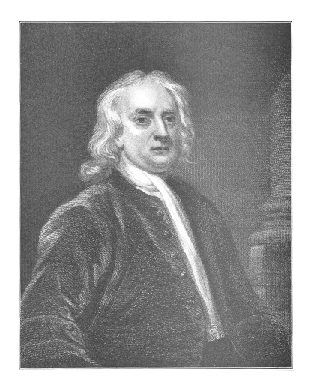
\includegraphics[height=6cm,width=4cm]{isaac-newton.eps}%
\lthtmlpictureZ
\lthtmlcheckvsize\clearpage}

{\newpage\clearpage
\lthtmlpictureA{tex2html_wrap42972}%
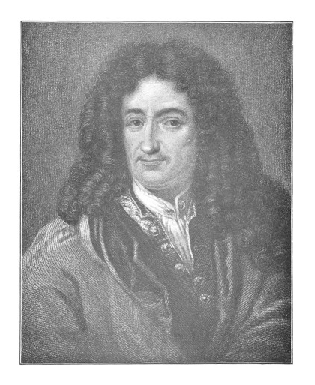
\includegraphics[height=6cm,width=4cm]{gottfried-wilhelm-leibnitz.eps}%
\lthtmlpictureZ
\lthtmlcheckvsize\clearpage}

\stepcounter{chapter}
\stepcounter{section}
{\newpage\clearpage
\lthtmlinlinemathA{tex2html_wrap_indisplay42985}%
$\displaystyle \begin{matrix} 
(a + b)^n = a^n + na^{n-1}b &+& \frac{n(n - 1)}{2!}a^{n-2}b^2 
+ \frac{n(n - 1)(n - 2)}{3!}a^{n-3}b^3 + \cdots \\
&+& \frac{n(n - 1)(n - 2)\cdots(n - r + 2)}{(r - 1)!}a^{n-r+1}b^{r-1} + \cdots 
\end{matrix}
$%
\lthtmlindisplaymathZ
\lthtmlcheckvsize\clearpage}

{\newpage\clearpage
\lthtmlinlinemathA{tex2html_wrap_inline42987}%
$ n! = 1 \cdot 2 \cdot 3 \cdot 4 \cdots (n - 1)n$%
\lthtmlinlinemathZ
\lthtmlcheckvsize\clearpage}

{\newpage\clearpage
\lthtmlinlinemathA{tex2html_wrap_inline42989}%
$ ax^2 + bx + c = 0$%
\lthtmlinlinemathZ
\lthtmlcheckvsize\clearpage}

{\newpage\clearpage
\lthtmlinlinemathA{tex2html_wrap_inline42991}%
$ b^2-4ac > 0$%
\lthtmlinlinemathZ
\lthtmlcheckvsize\clearpage}

{\newpage\clearpage
\lthtmlinlinemathA{tex2html_wrap_inline42993}%
$ b^2-4ac = 0$%
\lthtmlinlinemathZ
\lthtmlcheckvsize\clearpage}

{\newpage\clearpage
\lthtmlinlinemathA{tex2html_wrap_inline42995}%
$ b^2-4ac < 0$%
\lthtmlinlinemathZ
\lthtmlcheckvsize\clearpage}

{\newpage\clearpage
\lthtmlinlinemathA{tex2html_wrap_inline42997}%
$ x^2 + px + q = 0$%
\lthtmlinlinemathZ
\lthtmlcheckvsize\clearpage}

{\newpage\clearpage
\lthtmlinlinemathA{tex2html_wrap_inline42999}%
$ p$%
\lthtmlinlinemathZ
\lthtmlcheckvsize\clearpage}

{\newpage\clearpage
\lthtmlinlinemathA{tex2html_wrap_inline43001}%
$ q$%
\lthtmlinlinemathZ
\lthtmlcheckvsize\clearpage}

{\newpage\clearpage
\lthtmlinlinemathA{tex2html_wrap_inline43005}%
$ a+d$%
\lthtmlinlinemathZ
\lthtmlcheckvsize\clearpage}

{\newpage\clearpage
\lthtmlinlinemathA{tex2html_wrap_inline43007}%
$ a+2d$%
\lthtmlinlinemathZ
\lthtmlcheckvsize\clearpage}

{\newpage\clearpage
\lthtmlinlinemathA{tex2html_wrap_indisplay43009}%
$\displaystyle s = \sum_{i=0}^{n-1} a + id = \frac{n}{2}[2a + (n-1)d].
$%
\lthtmlindisplaymathZ
\lthtmlcheckvsize\clearpage}

{\newpage\clearpage
\lthtmlinlinemathA{tex2html_wrap_inline43013}%
$ ar$%
\lthtmlinlinemathZ
\lthtmlcheckvsize\clearpage}

{\newpage\clearpage
\lthtmlinlinemathA{tex2html_wrap_inline43015}%
$ ar^2$%
\lthtmlinlinemathZ
\lthtmlcheckvsize\clearpage}

{\newpage\clearpage
\lthtmlinlinemathA{tex2html_wrap_indisplay43017}%
$\displaystyle s = \sum_{i=0}^{n-1} ar^{i} = \frac{a(r^n - 1)}{r - 1}.
$%
\lthtmlindisplaymathZ
\lthtmlcheckvsize\clearpage}

{\newpage\clearpage
\lthtmlinlinemathA{tex2html_wrap_inline43019}%
$ \log ab = \log a + \log b$%
\lthtmlinlinemathZ
\lthtmlcheckvsize\clearpage}

{\newpage\clearpage
\lthtmlinlinemathA{tex2html_wrap_inline43021}%
$ \log \frac{a}{b} = \log a - \log b$%
\lthtmlinlinemathZ
\lthtmlcheckvsize\clearpage}

{\newpage\clearpage
\lthtmlinlinemathA{tex2html_wrap_inline43023}%
$ \log a^n = n\log a$%
\lthtmlinlinemathZ
\lthtmlcheckvsize\clearpage}

{\newpage\clearpage
\lthtmlinlinemathA{tex2html_wrap_inline43025}%
$ \log \sqrt[n]{a} = \frac{1}{n} \log a$%
\lthtmlinlinemathZ
\lthtmlcheckvsize\clearpage}

{\newpage\clearpage
\lthtmlinlinemathA{tex2html_wrap_inline43027}%
$ \log 1 = 0$%
\lthtmlinlinemathZ
\lthtmlcheckvsize\clearpage}

{\newpage\clearpage
\lthtmlinlinemathA{tex2html_wrap_inline43029}%
$ \log e = 1$%
\lthtmlinlinemathZ
\lthtmlcheckvsize\clearpage}

{\newpage\clearpage
\lthtmlinlinemathA{tex2html_wrap_inline43031}%
$ \log \frac{1}{a} = -\log a$%
\lthtmlinlinemathZ
\lthtmlcheckvsize\clearpage}

{\newpage\clearpage
\lthtmlinlinemathA{tex2html_wrap_inline43035}%
$ r$%
\lthtmlinlinemathZ
\lthtmlcheckvsize\clearpage}

{\newpage\clearpage
\lthtmlinlinemathA{tex2html_wrap_inline43041}%
$ s$%
\lthtmlinlinemathZ
\lthtmlcheckvsize\clearpage}

{\newpage\clearpage
\lthtmlinlinemathA{tex2html_wrap_inline43043}%
$ 2 \pi\, r$%
\lthtmlinlinemathZ
\lthtmlcheckvsize\clearpage}

{\newpage\clearpage
\lthtmlinlinemathA{tex2html_wrap_inline43045}%
$ \pi\, r^2$%
\lthtmlinlinemathZ
\lthtmlcheckvsize\clearpage}

{\newpage\clearpage
\lthtmlinlinemathA{tex2html_wrap_inline43047}%
$ Ba$%
\lthtmlinlinemathZ
\lthtmlcheckvsize\clearpage}

{\newpage\clearpage
\lthtmlinlinemathA{tex2html_wrap_inline43049}%
$ \frac{1}{3} Ba$%
\lthtmlinlinemathZ
\lthtmlcheckvsize\clearpage}

{\newpage\clearpage
\lthtmlinlinemathA{tex2html_wrap_inline43051}%
$ \pi\, r^2a$%
\lthtmlinlinemathZ
\lthtmlcheckvsize\clearpage}

{\newpage\clearpage
\lthtmlinlinemathA{tex2html_wrap_inline43053}%
$ 2 \pi\, ra$%
\lthtmlinlinemathZ
\lthtmlcheckvsize\clearpage}

{\newpage\clearpage
\lthtmlinlinemathA{tex2html_wrap_inline43055}%
$ 2 \pi\, r(r + a)$%
\lthtmlinlinemathZ
\lthtmlcheckvsize\clearpage}

{\newpage\clearpage
\lthtmlinlinemathA{tex2html_wrap_inline43059}%
$ \pi\  rs$%
\lthtmlinlinemathZ
\lthtmlcheckvsize\clearpage}

{\newpage\clearpage
\lthtmlinlinemathA{tex2html_wrap_inline43061}%
$ \pi\  r(r + s)$%
\lthtmlinlinemathZ
\lthtmlcheckvsize\clearpage}

{\newpage\clearpage
\lthtmlinlinemathA{tex2html_wrap_inline43063}%
$ \frac{4}{3}\pi\  r^3$%
\lthtmlinlinemathZ
\lthtmlcheckvsize\clearpage}

{\newpage\clearpage
\lthtmlinlinemathA{tex2html_wrap_inline43065}%
$ 4\pi\  r^2$%
\lthtmlinlinemathZ
\lthtmlcheckvsize\clearpage}

{\newpage\clearpage
\lthtmlinlinemathA{tex2html_wrap_inline43067}%
$ \sin x = \frac{1}{\csc x}$%
\lthtmlinlinemathZ
\lthtmlcheckvsize\clearpage}

{\newpage\clearpage
\lthtmlinlinemathA{tex2html_wrap_inline43069}%
$ \cos x = \frac{1}{\sec x}$%
\lthtmlinlinemathZ
\lthtmlcheckvsize\clearpage}

{\newpage\clearpage
\lthtmlinlinemathA{tex2html_wrap_inline43071}%
$ \tan x = \frac{1}{\cot x}$%
\lthtmlinlinemathZ
\lthtmlcheckvsize\clearpage}

{\newpage\clearpage
\lthtmlinlinemathA{tex2html_wrap_inline43073}%
$ \tan x = \frac{\sin{x}}{\cos{x}}$%
\lthtmlinlinemathZ
\lthtmlcheckvsize\clearpage}

{\newpage\clearpage
\lthtmlinlinemathA{tex2html_wrap_inline43075}%
$ \cot{x} = \frac{\cos{x}}{\sin{x}}$%
\lthtmlinlinemathZ
\lthtmlcheckvsize\clearpage}

{\newpage\clearpage
\lthtmlinlinemathA{tex2html_wrap_inline43077}%
$ \sin^2 x + \cos^2 x = 1$%
\lthtmlinlinemathZ
\lthtmlcheckvsize\clearpage}

{\newpage\clearpage
\lthtmlinlinemathA{tex2html_wrap_inline43079}%
$ 1 + \tan^2 x = \sec^2 x$%
\lthtmlinlinemathZ
\lthtmlcheckvsize\clearpage}

{\newpage\clearpage
\lthtmlinlinemathA{tex2html_wrap_inline43081}%
$ 1 + \cot^2 x = \csc^2 x$%
\lthtmlinlinemathZ
\lthtmlcheckvsize\clearpage}

{\newpage\clearpage
\lthtmlinlinemathA{tex2html_wrap_inline43083}%
$ \sin x = \cos \left ( \frac{\pi}{2} - x \right )$%
\lthtmlinlinemathZ
\lthtmlcheckvsize\clearpage}

{\newpage\clearpage
\lthtmlinlinemathA{tex2html_wrap_inline43085}%
$ \cos x = \sin \left ( \frac{\pi}{2} - x \right)$%
\lthtmlinlinemathZ
\lthtmlcheckvsize\clearpage}

{\newpage\clearpage
\lthtmlinlinemathA{tex2html_wrap_inline43087}%
$ \tan x = \cot \left ( \frac{\pi}{2} - x \right )$%
\lthtmlinlinemathZ
\lthtmlcheckvsize\clearpage}

{\newpage\clearpage
\lthtmlinlinemathA{tex2html_wrap_inline43089}%
$ \sin(\pi\  - x) = \sin x$%
\lthtmlinlinemathZ
\lthtmlcheckvsize\clearpage}

{\newpage\clearpage
\lthtmlinlinemathA{tex2html_wrap_inline43091}%
$ \cos(\pi\  - x) = -\cos x$%
\lthtmlinlinemathZ
\lthtmlcheckvsize\clearpage}

{\newpage\clearpage
\lthtmlinlinemathA{tex2html_wrap_inline43093}%
$ \tan(\pi\  - x) = -\tan x$%
\lthtmlinlinemathZ
\lthtmlcheckvsize\clearpage}

{\newpage\clearpage
\lthtmlinlinemathA{tex2html_wrap_inline43095}%
$ \sin (x + y) = \sin x \cos y + \cos x \sin y$%
\lthtmlinlinemathZ
\lthtmlcheckvsize\clearpage}

{\newpage\clearpage
\lthtmlinlinemathA{tex2html_wrap_inline43097}%
$ \sin (x-y) = \sin x \cos y-\cos x \sin y$%
\lthtmlinlinemathZ
\lthtmlcheckvsize\clearpage}

{\newpage\clearpage
\lthtmlinlinemathA{tex2html_wrap_inline43099}%
$ \cos(x \pm y) = \cos x \cos y +\mp \sin x \sin y$%
\lthtmlinlinemathZ
\lthtmlcheckvsize\clearpage}

{\newpage\clearpage
\lthtmlinlinemathA{tex2html_wrap_inline43101}%
$ \tan(x + y) = \frac{\tan x + \tan y}{1 - \tan x \tan y}$%
\lthtmlinlinemathZ
\lthtmlcheckvsize\clearpage}

{\newpage\clearpage
\lthtmlinlinemathA{tex2html_wrap_inline43103}%
$ \tan(x - y) = \frac{\tan x - \tan y}{1 + \tan x \tan y}$%
\lthtmlinlinemathZ
\lthtmlcheckvsize\clearpage}

{\newpage\clearpage
\lthtmlinlinemathA{tex2html_wrap_inline43105}%
$ \sin 2x = 2 \sin x \cos x$%
\lthtmlinlinemathZ
\lthtmlcheckvsize\clearpage}

{\newpage\clearpage
\lthtmlinlinemathA{tex2html_wrap_inline43107}%
$ \cos 2x = \cos^2 x - \sin^2 x$%
\lthtmlinlinemathZ
\lthtmlcheckvsize\clearpage}

{\newpage\clearpage
\lthtmlinlinemathA{tex2html_wrap_inline43109}%
$ \tan 2x = \frac{2 \tan x}{1 - \tan^2 x}$%
\lthtmlinlinemathZ
\lthtmlcheckvsize\clearpage}

{\newpage\clearpage
\lthtmlinlinemathA{tex2html_wrap_inline43111}%
$ \sin x = 2\sin \frac{x}{2} \cos \frac{x}{2}$%
\lthtmlinlinemathZ
\lthtmlcheckvsize\clearpage}

{\newpage\clearpage
\lthtmlinlinemathA{tex2html_wrap_inline43113}%
$ \cos x = \cos^2 \frac{x}{2} - \sin^2 \frac{x}{2}$%
\lthtmlinlinemathZ
\lthtmlcheckvsize\clearpage}

{\newpage\clearpage
\lthtmlinlinemathA{tex2html_wrap_inline43115}%
$ \tan x = \frac{2 \tan \frac{1}{2} x}{1 - \tan^2 \frac{1}{2} x}$%
\lthtmlinlinemathZ
\lthtmlcheckvsize\clearpage}

{\newpage\clearpage
\lthtmlinlinemathA{tex2html_wrap_inline43117}%
$ \cos^2 x = \frac{1}{2} + \frac{1}{2} \cos 2x$%
\lthtmlinlinemathZ
\lthtmlcheckvsize\clearpage}

{\newpage\clearpage
\lthtmlinlinemathA{tex2html_wrap_inline43119}%
$ \sin^2 x = \frac{1}{2} - \frac{1}{2} \cos 2x$%
\lthtmlinlinemathZ
\lthtmlcheckvsize\clearpage}

{\newpage\clearpage
\lthtmlinlinemathA{tex2html_wrap_inline43121}%
$ 1 + \cos x = 2 \cos^2 \frac{x}{2}$%
\lthtmlinlinemathZ
\lthtmlcheckvsize\clearpage}

{\newpage\clearpage
\lthtmlinlinemathA{tex2html_wrap_inline43123}%
$ 1 - \cos x = 2 \sin^2 \frac{x}{2}$%
\lthtmlinlinemathZ
\lthtmlcheckvsize\clearpage}

{\newpage\clearpage
\lthtmlinlinemathA{tex2html_wrap_inline43125}%
$ \sin \frac{x}{2} = \pm \sqrt{ \frac{1 - \cos x}{2} }$%
\lthtmlinlinemathZ
\lthtmlcheckvsize\clearpage}

{\newpage\clearpage
\lthtmlinlinemathA{tex2html_wrap_inline43127}%
$ \cos x/2 = \pm \sqrt{ \frac{1 + \cos x}{2} }$%
\lthtmlinlinemathZ
\lthtmlcheckvsize\clearpage}

{\newpage\clearpage
\lthtmlinlinemathA{tex2html_wrap_inline43129}%
$ \tan \frac{x}{2} = \pm \sqrt{ \frac{1 - \cos x}{1 + \cos x}}$%
\lthtmlinlinemathZ
\lthtmlcheckvsize\clearpage}

{\newpage\clearpage
\lthtmlinlinemathA{tex2html_wrap_inline43131}%
$ \sin x + \sin y = 2 \sin \frac{1}{2} (x + y) cos \frac{1}{2} (x - y)$%
\lthtmlinlinemathZ
\lthtmlcheckvsize\clearpage}

{\newpage\clearpage
\lthtmlinlinemathA{tex2html_wrap_inline43133}%
$ \sin x - \sin y = 2 \cos \frac{1}{2} (x + y) sin \frac{1}{2} (x - y)$%
\lthtmlinlinemathZ
\lthtmlcheckvsize\clearpage}

{\newpage\clearpage
\lthtmlinlinemathA{tex2html_wrap_inline43135}%
$ \cos x + \cos y = -2 \cos \frac{1}{2} (x + y) cos \frac{1}{2} (x - y)$%
\lthtmlinlinemathZ
\lthtmlcheckvsize\clearpage}

{\newpage\clearpage
\lthtmlinlinemathA{tex2html_wrap_inline43137}%
$ \cos x - \cos y = -2 \sin \frac{1}{2} (x + y) sin \frac{1}{2} (x - y)$%
\lthtmlinlinemathZ
\lthtmlcheckvsize\clearpage}

{\newpage\clearpage
\lthtmlinlinemathA{tex2html_wrap_inline43139}%
$ \frac{a}{\sin A} = \frac{b}{\sin B} = \frac{c}{\sin C}$%
\lthtmlinlinemathZ
\lthtmlcheckvsize\clearpage}

{\newpage\clearpage
\lthtmlinlinemathA{tex2html_wrap_inline43141}%
$ a^2 = b^2 + c^2 − 2bc\cos A$%
\lthtmlinlinemathZ
\lthtmlcheckvsize\clearpage}

{\newpage\clearpage
\lthtmlinlinemathA{tex2html_wrap_inline43143}%
$ d = \sqrt{ (x_1 - x_2)^2 + (y_1 - y_2)^2}$%
\lthtmlinlinemathZ
\lthtmlcheckvsize\clearpage}

{\newpage\clearpage
\lthtmlinlinemathA{tex2html_wrap_inline43145}%
$ (x_1,y_1)$%
\lthtmlinlinemathZ
\lthtmlcheckvsize\clearpage}

{\newpage\clearpage
\lthtmlinlinemathA{tex2html_wrap_inline43147}%
$ (x_2,y_2)$%
\lthtmlinlinemathZ
\lthtmlcheckvsize\clearpage}

{\newpage\clearpage
\lthtmlinlinemathA{tex2html_wrap_inline43149}%
$ d = \frac{Ax_1 + By_1 + C}{\pm \sqrt{A^2 + B^2}}$%
\lthtmlinlinemathZ
\lthtmlcheckvsize\clearpage}

{\newpage\clearpage
\lthtmlinlinemathA{tex2html_wrap_inline43151}%
$ Ax + By + C = 0$%
\lthtmlinlinemathZ
\lthtmlcheckvsize\clearpage}

{\newpage\clearpage
\lthtmlinlinemathA{tex2html_wrap_inline43155}%
$ x = \frac{x_1 + x_2}{2}$%
\lthtmlinlinemathZ
\lthtmlcheckvsize\clearpage}

{\newpage\clearpage
\lthtmlinlinemathA{tex2html_wrap_inline43157}%
$ y = \frac{y_1 + y_2}{2}$%
\lthtmlinlinemathZ
\lthtmlcheckvsize\clearpage}

{\newpage\clearpage
\lthtmlinlinemathA{tex2html_wrap_inline43159}%
$ x = x_0 + x'$%
\lthtmlinlinemathZ
\lthtmlcheckvsize\clearpage}

{\newpage\clearpage
\lthtmlinlinemathA{tex2html_wrap_inline43161}%
$ y = y_0 + y'$%
\lthtmlinlinemathZ
\lthtmlcheckvsize\clearpage}

{\newpage\clearpage
\lthtmlinlinemathA{tex2html_wrap_inline43163}%
$ (x_0,y_0)$%
\lthtmlinlinemathZ
\lthtmlcheckvsize\clearpage}

{\newpage\clearpage
\lthtmlinlinemathA{tex2html_wrap_inline43165}%
$ x = x' \cos \theta\  - y' \sin \theta\  $%
\lthtmlinlinemathZ
\lthtmlcheckvsize\clearpage}

{\newpage\clearpage
\lthtmlinlinemathA{tex2html_wrap_inline43167}%
$ y = x' \sin \theta\  + y' \cos \theta$%
\lthtmlinlinemathZ
\lthtmlcheckvsize\clearpage}

{\newpage\clearpage
\lthtmlinlinemathA{tex2html_wrap_inline43169}%
$ x = \rho\  \cos \theta\  $%
\lthtmlinlinemathZ
\lthtmlcheckvsize\clearpage}

{\newpage\clearpage
\lthtmlinlinemathA{tex2html_wrap_inline43171}%
$ y = \rho\  \sin \theta$%
\lthtmlinlinemathZ
\lthtmlcheckvsize\clearpage}

{\newpage\clearpage
\lthtmlinlinemathA{tex2html_wrap_inline43173}%
$ \rho\  = \sqrt{x^2 + y^2}$%
\lthtmlinlinemathZ
\lthtmlcheckvsize\clearpage}

{\newpage\clearpage
\lthtmlinlinemathA{tex2html_wrap_inline43175}%
$ \theta\  = \arctan \frac{y}{x}$%
\lthtmlinlinemathZ
\lthtmlcheckvsize\clearpage}

{\newpage\clearpage
\lthtmlinlinemathA{tex2html_wrap_inline43183}%
$ \frac{y - y_1}{x - x_1} = \frac{y_2 - y_1}{x_2 - x_1}$%
\lthtmlinlinemathZ
\lthtmlcheckvsize\clearpage}

{\newpage\clearpage
\lthtmlinlinemathA{tex2html_wrap_inline43185}%
$ \frac{x}{a} + \frac{y}{b} = 1$%
\lthtmlinlinemathZ
\lthtmlcheckvsize\clearpage}

{\newpage\clearpage
\lthtmlinlinemathA{tex2html_wrap_inline43187}%
$ y-y_1 = m(x-x_1)$%
\lthtmlinlinemathZ
\lthtmlcheckvsize\clearpage}

{\newpage\clearpage
\lthtmlinlinemathA{tex2html_wrap_inline43189}%
$ y = mx + b$%
\lthtmlinlinemathZ
\lthtmlcheckvsize\clearpage}

{\newpage\clearpage
\lthtmlinlinemathA{tex2html_wrap_inline43191}%
$ x \cos \alpha\  + y \sin \alpha\  = p$%
\lthtmlinlinemathZ
\lthtmlcheckvsize\clearpage}

{\newpage\clearpage
\lthtmlinlinemathA{tex2html_wrap_inline43201}%
$ \tan \theta\  = \frac{m_1 - m_2}{1 + m_1 m_2}$%
\lthtmlinlinemathZ
\lthtmlcheckvsize\clearpage}

{\newpage\clearpage
\lthtmlinlinemathA{tex2html_wrap_inline43203}%
$ m_1$%
\lthtmlinlinemathZ
\lthtmlcheckvsize\clearpage}

{\newpage\clearpage
\lthtmlinlinemathA{tex2html_wrap_inline43205}%
$ m_2$%
\lthtmlinlinemathZ
\lthtmlcheckvsize\clearpage}

{\newpage\clearpage
\lthtmlinlinemathA{tex2html_wrap_inline43207}%
$ m_1 = m_2$%
\lthtmlinlinemathZ
\lthtmlcheckvsize\clearpage}

{\newpage\clearpage
\lthtmlinlinemathA{tex2html_wrap_inline43209}%
$ m_1 = -\frac{1}{m_2}$%
\lthtmlinlinemathZ
\lthtmlcheckvsize\clearpage}

{\newpage\clearpage
\lthtmlinlinemathA{tex2html_wrap_inline43211}%
$ (x - \alpha)^2 + (y - \beta)^2 = r^2$%
\lthtmlinlinemathZ
\lthtmlcheckvsize\clearpage}

{\newpage\clearpage
\lthtmlinlinemathA{tex2html_wrap_inline43213}%
$ (\alpha,\beta)$%
\lthtmlinlinemathZ
\lthtmlcheckvsize\clearpage}

\stepcounter{section}
{\newpage\clearpage
\lthtmlinlinemathA{tex2html_wrap_inline43218}%
$ A,\alpha$%
\lthtmlinlinemathZ
\lthtmlcheckvsize\clearpage}

{\newpage\clearpage
\lthtmlinlinemathA{tex2html_wrap_inline43220}%
$ N, \nu$%
\lthtmlinlinemathZ
\lthtmlcheckvsize\clearpage}

{\newpage\clearpage
\lthtmlinlinemathA{tex2html_wrap_inline43222}%
$ B,\beta$%
\lthtmlinlinemathZ
\lthtmlcheckvsize\clearpage}

{\newpage\clearpage
\lthtmlinlinemathA{tex2html_wrap_inline43224}%
$ \Xi,\xi$%
\lthtmlinlinemathZ
\lthtmlcheckvsize\clearpage}

{\newpage\clearpage
\lthtmlinlinemathA{tex2html_wrap_inline43226}%
$ \Gamma, \gamma$%
\lthtmlinlinemathZ
\lthtmlcheckvsize\clearpage}

{\newpage\clearpage
\lthtmlinlinemathA{tex2html_wrap_inline43228}%
$ O,o$%
\lthtmlinlinemathZ
\lthtmlcheckvsize\clearpage}

{\newpage\clearpage
\lthtmlinlinemathA{tex2html_wrap_inline43230}%
$ \Delta,\delta$%
\lthtmlinlinemathZ
\lthtmlcheckvsize\clearpage}

{\newpage\clearpage
\lthtmlinlinemathA{tex2html_wrap_inline43232}%
$ \Pi,\pi$%
\lthtmlinlinemathZ
\lthtmlcheckvsize\clearpage}

{\newpage\clearpage
\lthtmlinlinemathA{tex2html_wrap_inline43234}%
$ E,\epsilon$%
\lthtmlinlinemathZ
\lthtmlcheckvsize\clearpage}

{\newpage\clearpage
\lthtmlinlinemathA{tex2html_wrap_inline43236}%
$ P,\rho$%
\lthtmlinlinemathZ
\lthtmlcheckvsize\clearpage}

{\newpage\clearpage
\lthtmlinlinemathA{tex2html_wrap_inline43238}%
$ Z,\zeta$%
\lthtmlinlinemathZ
\lthtmlcheckvsize\clearpage}

{\newpage\clearpage
\lthtmlinlinemathA{tex2html_wrap_inline43240}%
$ \Sigma,\sigma$%
\lthtmlinlinemathZ
\lthtmlcheckvsize\clearpage}

{\newpage\clearpage
\lthtmlinlinemathA{tex2html_wrap_inline43242}%
$ H,\eta$%
\lthtmlinlinemathZ
\lthtmlcheckvsize\clearpage}

{\newpage\clearpage
\lthtmlinlinemathA{tex2html_wrap_inline43244}%
$ T,\tau$%
\lthtmlinlinemathZ
\lthtmlcheckvsize\clearpage}

{\newpage\clearpage
\lthtmlinlinemathA{tex2html_wrap_inline43246}%
$ \Theta,\theta$%
\lthtmlinlinemathZ
\lthtmlcheckvsize\clearpage}

{\newpage\clearpage
\lthtmlinlinemathA{tex2html_wrap_inline43248}%
$ Y,\upsilon$%
\lthtmlinlinemathZ
\lthtmlcheckvsize\clearpage}

{\newpage\clearpage
\lthtmlinlinemathA{tex2html_wrap_inline43250}%
$ I,\iota$%
\lthtmlinlinemathZ
\lthtmlcheckvsize\clearpage}

{\newpage\clearpage
\lthtmlinlinemathA{tex2html_wrap_inline43252}%
$ \Phi,\phi$%
\lthtmlinlinemathZ
\lthtmlcheckvsize\clearpage}

{\newpage\clearpage
\lthtmlinlinemathA{tex2html_wrap_inline43254}%
$ K,\kappa$%
\lthtmlinlinemathZ
\lthtmlcheckvsize\clearpage}

{\newpage\clearpage
\lthtmlinlinemathA{tex2html_wrap_inline43256}%
$ X,\chi$%
\lthtmlinlinemathZ
\lthtmlcheckvsize\clearpage}

{\newpage\clearpage
\lthtmlinlinemathA{tex2html_wrap_inline43258}%
$ \Lambda,\lambda$%
\lthtmlinlinemathZ
\lthtmlcheckvsize\clearpage}

{\newpage\clearpage
\lthtmlinlinemathA{tex2html_wrap_inline43260}%
$ \Psi,\psi$%
\lthtmlinlinemathZ
\lthtmlcheckvsize\clearpage}

{\newpage\clearpage
\lthtmlinlinemathA{tex2html_wrap_inline43262}%
$ M,\mu$%
\lthtmlinlinemathZ
\lthtmlcheckvsize\clearpage}

{\newpage\clearpage
\lthtmlinlinemathA{tex2html_wrap_inline43264}%
$ \Omega,\omega$%
\lthtmlinlinemathZ
\lthtmlcheckvsize\clearpage}

\stepcounter{section}
\stepcounter{section}
{\newpage\clearpage
\lthtmlinlinemathA{tex2html_wrap_inline43359}%
$ \frac{\pi}{6}$%
\lthtmlinlinemathZ
\lthtmlcheckvsize\clearpage}

{\newpage\clearpage
\lthtmlinlinemathA{tex2html_wrap_inline43361}%
$ \frac{1}{2}$%
\lthtmlinlinemathZ
\lthtmlcheckvsize\clearpage}

{\newpage\clearpage
\lthtmlinlinemathA{tex2html_wrap_inline43363}%
$ \frac{\sqrt{3}}{2}$%
\lthtmlinlinemathZ
\lthtmlcheckvsize\clearpage}

{\newpage\clearpage
\lthtmlinlinemathA{tex2html_wrap_inline43365}%
$ \frac{\sqrt{3}}{3}$%
\lthtmlinlinemathZ
\lthtmlcheckvsize\clearpage}

{\newpage\clearpage
\lthtmlinlinemathA{tex2html_wrap_inline43367}%
$ \sqrt{3}$%
\lthtmlinlinemathZ
\lthtmlcheckvsize\clearpage}

{\newpage\clearpage
\lthtmlinlinemathA{tex2html_wrap_inline43369}%
$ \frac{2\sqrt{3}}{3}$%
\lthtmlinlinemathZ
\lthtmlcheckvsize\clearpage}

{\newpage\clearpage
\lthtmlinlinemathA{tex2html_wrap_inline43371}%
$ 2$%
\lthtmlinlinemathZ
\lthtmlcheckvsize\clearpage}

{\newpage\clearpage
\lthtmlinlinemathA{tex2html_wrap_inline43373}%
$ \frac{\pi}{4}$%
\lthtmlinlinemathZ
\lthtmlcheckvsize\clearpage}

{\newpage\clearpage
\lthtmlinlinemathA{tex2html_wrap_inline43375}%
$ 45$%
\lthtmlinlinemathZ
\lthtmlcheckvsize\clearpage}

{\newpage\clearpage
\lthtmlinlinemathA{tex2html_wrap_inline43377}%
$ \frac{\sqrt{2}}{2}$%
\lthtmlinlinemathZ
\lthtmlcheckvsize\clearpage}

{\newpage\clearpage
\lthtmlinlinemathA{tex2html_wrap_inline43381}%
$ \sqrt{2}$%
\lthtmlinlinemathZ
\lthtmlcheckvsize\clearpage}

{\newpage\clearpage
\lthtmlinlinemathA{tex2html_wrap_inline43385}%
$ \frac{\pi}{3}$%
\lthtmlinlinemathZ
\lthtmlcheckvsize\clearpage}

{\newpage\clearpage
\lthtmlinlinemathA{tex2html_wrap_inline43397}%
$ \frac{\pi}{2}$%
\lthtmlinlinemathZ
\lthtmlcheckvsize\clearpage}

{\newpage\clearpage
\lthtmlinlinemathA{tex2html_wrap_inline43403}%
$ \pi$%
\lthtmlinlinemathZ
\lthtmlcheckvsize\clearpage}

{\newpage\clearpage
\lthtmlinlinemathA{tex2html_wrap_inline43409}%
$ \frac{3\pi}{2}$%
\lthtmlinlinemathZ
\lthtmlcheckvsize\clearpage}

{\newpage\clearpage
\lthtmlinlinemathA{tex2html_wrap_inline43415}%
$ 2\pi$%
\lthtmlinlinemathZ
\lthtmlcheckvsize\clearpage}

{\newpage\clearpage
\lthtmlinlinemathA{tex2html_wrap_inline43645}%
$ \sin(x)$%
\lthtmlinlinemathZ
\lthtmlcheckvsize\clearpage}

{\newpage\clearpage
\lthtmlinlinemathA{tex2html_wrap_inline43647}%
$ x\in \{0.01750, 0.03500, ... %0.05250, 0.07000, 0.08750, 0.1750, 0.2625, 
0.7875\}$%
\lthtmlinlinemathZ
\lthtmlcheckvsize\clearpage}

{\newpage\clearpage
\lthtmlinlinemathA{tex2html_wrap_inline43649}%
$ \cos$%
\lthtmlinlinemathZ
\lthtmlcheckvsize\clearpage}

{\newpage\clearpage
\lthtmlinlinemathA{tex2html_wrap_inline43651}%
$ \tan$%
\lthtmlinlinemathZ
\lthtmlcheckvsize\clearpage}

{\newpage\clearpage
\lthtmlinlinemathA{tex2html_wrap_inline43653}%
$ \cot$%
\lthtmlinlinemathZ
\lthtmlcheckvsize\clearpage}

\stepcounter{section}
{\newpage\clearpage
\lthtmlinlinemathA{tex2html_wrap_inline43660}%
$ x=120$%
\lthtmlinlinemathZ
\lthtmlcheckvsize\clearpage}

{\newpage\clearpage
\lthtmlinlinemathA{tex2html_wrap_indisplay43662}%
$\displaystyle \log_{10}120=\log_{10}(10^2\times 1.2)=2+\log_{10}1.2\approx2+0.079181.
$%
\lthtmlindisplaymathZ
\lthtmlcheckvsize\clearpage}

{\newpage\clearpage
\lthtmlinlinemathA{tex2html_wrap_inline43664}%
$ 0.079181...$%
\lthtmlinlinemathZ
\lthtmlcheckvsize\clearpage}

{\newpage\clearpage
\lthtmlinlinemathA{tex2html_wrap_inline43666}%
$ 0792$%
\lthtmlinlinemathZ
\lthtmlcheckvsize\clearpage}

\stepcounter{chapter}
\stepcounter{section}
{\newpage\clearpage
\lthtmlinlinemathA{tex2html_wrap_indisplay43890}%
$\displaystyle \frac{x}{a} + \frac{y}{b} = 1
$%
\lthtmlindisplaymathZ
\lthtmlcheckvsize\clearpage}

{\newpage\clearpage
\lthtmlinlinemathA{tex2html_wrap_inline43898}%
$ 5$%
\lthtmlinlinemathZ
\lthtmlcheckvsize\clearpage}

{\newpage\clearpage
\lthtmlinlinemathA{tex2html_wrap_inline43900}%
$ \sqrt{7}$%
\lthtmlinlinemathZ
\lthtmlcheckvsize\clearpage}

{\newpage\clearpage
\lthtmlinlinemathA{tex2html_wrap_inline43906}%
$ b$%
\lthtmlinlinemathZ
\lthtmlcheckvsize\clearpage}

\stepcounter{section}
{\newpage\clearpage
\lthtmlinlinemathA{tex2html_wrap_inline43919}%
$ \left \lbrack a,\  b \right \rbrack$%
\lthtmlinlinemathZ
\lthtmlcheckvsize\clearpage}

{\newpage\clearpage
\lthtmlinlinemathA{tex2html_wrap_inline43925}%
$ a,\  b$%
\lthtmlinlinemathZ
\lthtmlcheckvsize\clearpage}

\stepcounter{section}
{\newpage\clearpage
\lthtmlpictureA{tex2html_wrap43948}%
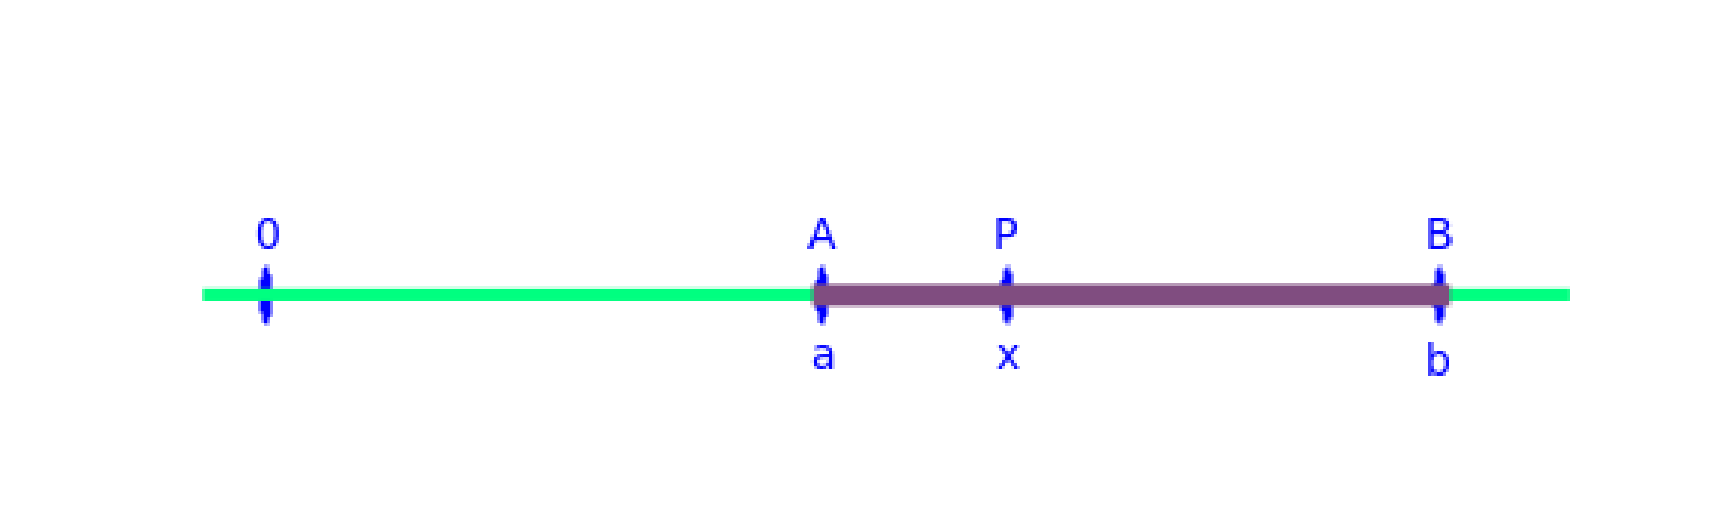
\includegraphics[height=2.5cm,width=8cm]{line-segment.eps}%
\lthtmlpictureZ
\lthtmlcheckvsize\clearpage}

{\newpage\clearpage
\lthtmlinlinemathA{tex2html_wrap_inline43961}%
$ O$%
\lthtmlinlinemathZ
\lthtmlcheckvsize\clearpage}

{\newpage\clearpage
\lthtmlinlinemathA{tex2html_wrap_inline43971}%
$ P$%
\lthtmlinlinemathZ
\lthtmlcheckvsize\clearpage}

{\newpage\clearpage
\lthtmlinlinemathA{tex2html_wrap_inline43977}%
$ AB$%
\lthtmlinlinemathZ
\lthtmlcheckvsize\clearpage}

\stepcounter{section}
\stepcounter{section}
\stepcounter{section}
{\newpage\clearpage
\lthtmlinlinemathA{tex2html_wrap_inline43998}%
$ f$%
\lthtmlinlinemathZ
\lthtmlcheckvsize\clearpage}

{\newpage\clearpage
\lthtmlinlinemathA{tex2html_wrap_inline44004}%
$ \phi(x)$%
\lthtmlinlinemathZ
\lthtmlcheckvsize\clearpage}

{\newpage\clearpage
\lthtmlinlinemathA{tex2html_wrap_inline44006}%
$ f'(x)$%
\lthtmlinlinemathZ
\lthtmlcheckvsize\clearpage}

{\newpage\clearpage
\lthtmlinlinemathA{tex2html_wrap_indisplay44008}%
$\displaystyle f(x) = x^2 - 9x + 14,
$%
\lthtmlindisplaymathZ
\lthtmlcheckvsize\clearpage}

{\newpage\clearpage
\lthtmlinlinemathA{tex2html_wrap_indisplay44010}%
$\displaystyle f(y) 	= y^2 - 9y + 14.
$%
\lthtmlindisplaymathZ
\lthtmlcheckvsize\clearpage}

{\newpage\clearpage
\lthtmlinlinemathA{tex2html_wrap_indisplay44012}%
$\displaystyle f(a) 	= a^2 - 9a + 14,
$%
\lthtmlindisplaymathZ
\lthtmlcheckvsize\clearpage}

{\newpage\clearpage
\lthtmlinlinemathA{tex2html_wrap_indisplay44014}%
$\displaystyle f(b + 1) = (b + 1)^2 - 9(b + 1) + 14 = b^2 - 7b + 6,
$%
\lthtmlindisplaymathZ
\lthtmlcheckvsize\clearpage}

{\newpage\clearpage
\lthtmlinlinemathA{tex2html_wrap_indisplay44016}%
$\displaystyle f(0) 	= 0^2 - 9 \cdot 0 + 14 = 14,
$%
\lthtmlindisplaymathZ
\lthtmlcheckvsize\clearpage}

{\newpage\clearpage
\lthtmlinlinemathA{tex2html_wrap_indisplay44018}%
$\displaystyle f(-1) 	= (-1)^2 -9(-1) + 14 = 24,
$%
\lthtmlindisplaymathZ
\lthtmlcheckvsize\clearpage}

{\newpage\clearpage
\lthtmlinlinemathA{tex2html_wrap_indisplay44020}%
$\displaystyle f(3) 	= 3^2 -9 \cdot 3 + 14 = -4,
$%
\lthtmlindisplaymathZ
\lthtmlcheckvsize\clearpage}

{\newpage\clearpage
\lthtmlinlinemathA{tex2html_wrap_indisplay44022}%
$\displaystyle f(7) 	= 7^2 -9 \cdot 7 + 14 = 0,
$%
\lthtmlindisplaymathZ
\lthtmlcheckvsize\clearpage}

{\newpage\clearpage
\lthtmlinlinemathA{tex2html_wrap_inline44024}%
$ \phi(x,\  y)$%
\lthtmlinlinemathZ
\lthtmlcheckvsize\clearpage}

{\newpage\clearpage
\lthtmlinlinemathA{tex2html_wrap_inline44030}%
$ \phi$%
\lthtmlinlinemathZ
\lthtmlcheckvsize\clearpage}

{\newpage\clearpage
\lthtmlinlinemathA{tex2html_wrap_indisplay44036}%
$\displaystyle \phi(x,\  y) 	= \sin(x + y),
$%
\lthtmlindisplaymathZ
\lthtmlcheckvsize\clearpage}

{\newpage\clearpage
\lthtmlinlinemathA{tex2html_wrap_indisplay44038}%
$\displaystyle \phi(a,\  b) 	= \sin(a + b),
$%
\lthtmlindisplaymathZ
\lthtmlcheckvsize\clearpage}

{\newpage\clearpage
\lthtmlinlinemathA{tex2html_wrap_indisplay44040}%
$\displaystyle \phi \left ( \frac{\pi}{2}, 0 \right )	= \sin \frac{\pi}{2} = 1.
$%
\lthtmlindisplaymathZ
\lthtmlcheckvsize\clearpage}

{\newpage\clearpage
\lthtmlinlinemathA{tex2html_wrap_indisplay44042}%
$\displaystyle F( x,\  y,\  z ) 	= 2x + 3y - 12z,
$%
\lthtmlindisplaymathZ
\lthtmlcheckvsize\clearpage}

{\newpage\clearpage
\lthtmlinlinemathA{tex2html_wrap_indisplay44044}%
$\displaystyle F(m,\  -m,\  m) 	= 2m - 3m - 12m = - 13m.
$%
\lthtmlindisplaymathZ
\lthtmlcheckvsize\clearpage}

{\newpage\clearpage
\lthtmlinlinemathA{tex2html_wrap_indisplay44046}%
$\displaystyle F(3,\  2,\  1) 	= 2 \cdot 3 + 3 \cdot 2 - 12 \cdot 1 = 0.
$%
\lthtmlindisplaymathZ
\lthtmlcheckvsize\clearpage}

\stepcounter{section}
{\newpage\clearpage
\lthtmlinlinemathA{tex2html_wrap_indisplay44049}%
$\displaystyle x^2 - 2x + 5,\  \sin x,\  \arctan x
$%
\lthtmlindisplaymathZ
\lthtmlcheckvsize\clearpage}

{\newpage\clearpage
\lthtmlinlinemathA{tex2html_wrap_indisplay44055}%
$\displaystyle y = x^2 - 2 x + 5,\  y = \sin x,\  y = \arctan x.
$%
\lthtmlindisplaymathZ
\lthtmlcheckvsize\clearpage}

{\newpage\clearpage
\lthtmlinlinemathA{tex2html_wrap_indisplay44061}%
$\displaystyle y = \frac{a}{x - b}$%
\lthtmlindisplaymathZ
\lthtmlcheckvsize\clearpage}

{\newpage\clearpage
\lthtmlinlinemathA{tex2html_wrap_inline44067}%
$ x = b$%
\lthtmlinlinemathZ
\lthtmlcheckvsize\clearpage}

{\newpage\clearpage
\lthtmlinlinemathA{tex2html_wrap_indisplay44073}%
$\displaystyle y = \sqrt{x}.$%
\lthtmlindisplaymathZ
\lthtmlcheckvsize\clearpage}

{\newpage\clearpage
\lthtmlinlinemathA{tex2html_wrap_indisplay44081}%
$\displaystyle y = \log_a{x}. \qquad a > 0$%
\lthtmlindisplaymathZ
\lthtmlcheckvsize\clearpage}

{\newpage\clearpage
\lthtmlinlinemathA{tex2html_wrap_indisplay44089}%
$\displaystyle y = \arcsin x,\  y = \arccos x.$%
\lthtmlindisplaymathZ
\lthtmlcheckvsize\clearpage}

{\newpage\clearpage
\lthtmlinlinemathA{tex2html_wrap_inline44091}%
$ +1$%
\lthtmlinlinemathZ
\lthtmlcheckvsize\clearpage}

{\newpage\clearpage
\lthtmlinlinemathA{tex2html_wrap_inline44093}%
$ -1$%
\lthtmlinlinemathZ
\lthtmlcheckvsize\clearpage}

\stepcounter{section}
{\newpage\clearpage
\lthtmlinlinemathA{tex2html_wrap_inline44102}%
$ f(x) = x^3 - 10x^2 + 31x - 30$%
\lthtmlinlinemathZ
\lthtmlcheckvsize\clearpage}

{\newpage\clearpage
\lthtmlinlinemathA{tex2html_wrap_indisplay44104}%
$\displaystyle f(0) 	= -30,\  \ \  \ f(y) = y^3 - 10y^2 + 31y - 30,
$%
\lthtmlindisplaymathZ
\lthtmlcheckvsize\clearpage}

{\newpage\clearpage
\lthtmlinlinemathA{tex2html_wrap_indisplay44106}%
$\displaystyle f(2) = 0,\  \ \  \  f(a) 	= a^3 - 10a^2 + 31a - 30,
$%
\lthtmlindisplaymathZ
\lthtmlcheckvsize\clearpage}

{\newpage\clearpage
\lthtmlinlinemathA{tex2html_wrap_indisplay44108}%
$\displaystyle f(3) =	f(5),\  \ \  \ 
f(yz) 	= y^3z^3 - 10y^2z^2 + 31yz - 30,
$%
\lthtmlindisplaymathZ
\lthtmlcheckvsize\clearpage}

{\newpage\clearpage
\lthtmlinlinemathA{tex2html_wrap_indisplay44110}%
$\displaystyle f(1) > f( − 3),\  \ \  \ 
f(x − 2) 	= x^3 - 16x^2 + 83x - 140,
$%
\lthtmlindisplaymathZ
\lthtmlcheckvsize\clearpage}

{\newpage\clearpage
\lthtmlinlinemathA{tex2html_wrap_indisplay44112}%
$\displaystyle f( - 1) 	= 6f(6). 
$%
\lthtmlindisplaymathZ
\lthtmlcheckvsize\clearpage}

{\newpage\clearpage
\lthtmlinlinemathA{tex2html_wrap_inline44114}%
$ f(x) = x^3 - 3x + 2$%
\lthtmlinlinemathZ
\lthtmlcheckvsize\clearpage}

{\newpage\clearpage
\lthtmlinlinemathA{tex2html_wrap_inline44116}%
$ f(0)$%
\lthtmlinlinemathZ
\lthtmlcheckvsize\clearpage}

{\newpage\clearpage
\lthtmlinlinemathA{tex2html_wrap_inline44118}%
$ f(1)$%
\lthtmlinlinemathZ
\lthtmlcheckvsize\clearpage}

{\newpage\clearpage
\lthtmlinlinemathA{tex2html_wrap_inline44120}%
$ f(-1)$%
\lthtmlinlinemathZ
\lthtmlcheckvsize\clearpage}

{\newpage\clearpage
\lthtmlinlinemathA{tex2html_wrap_inline44122}%
$ f \left ( -\frac{1}{2} \right )$%
\lthtmlinlinemathZ
\lthtmlcheckvsize\clearpage}

{\newpage\clearpage
\lthtmlinlinemathA{tex2html_wrap_inline44124}%
$ f \left ( \frac{4}{3} \right )$%
\lthtmlinlinemathZ
\lthtmlcheckvsize\clearpage}

{\newpage\clearpage
\lthtmlinlinemathA{tex2html_wrap_inline44128}%
$ \phi (x) = x^4 − 55x^2 − 210x − 216$%
\lthtmlinlinemathZ
\lthtmlcheckvsize\clearpage}

{\newpage\clearpage
\lthtmlinlinemathA{tex2html_wrap_inline44130}%
$ f(2) = \phi ( - 2)$%
\lthtmlinlinemathZ
\lthtmlcheckvsize\clearpage}

{\newpage\clearpage
\lthtmlinlinemathA{tex2html_wrap_inline44132}%
$ f(3) = \phi( - 3),f(5) = \phi( - 4)$%
\lthtmlinlinemathZ
\lthtmlcheckvsize\clearpage}

{\newpage\clearpage
\lthtmlinlinemathA{tex2html_wrap_inline44134}%
$ f(0) + \phi (0) + 246 = 0$%
\lthtmlinlinemathZ
\lthtmlcheckvsize\clearpage}

{\newpage\clearpage
\lthtmlinlinemathA{tex2html_wrap_inline44136}%
$ F(x) = 2x$%
\lthtmlinlinemathZ
\lthtmlcheckvsize\clearpage}

{\newpage\clearpage
\lthtmlinlinemathA{tex2html_wrap_inline44138}%
$ F(0)$%
\lthtmlinlinemathZ
\lthtmlcheckvsize\clearpage}

{\newpage\clearpage
\lthtmlinlinemathA{tex2html_wrap_inline44140}%
$ F(-3)$%
\lthtmlinlinemathZ
\lthtmlcheckvsize\clearpage}

{\newpage\clearpage
\lthtmlinlinemathA{tex2html_wrap_inline44142}%
$ F \left ( \frac{1}{3} \right )$%
\lthtmlinlinemathZ
\lthtmlcheckvsize\clearpage}

{\newpage\clearpage
\lthtmlinlinemathA{tex2html_wrap_inline44144}%
$ F(-1)$%
\lthtmlinlinemathZ
\lthtmlcheckvsize\clearpage}

{\newpage\clearpage
\lthtmlinlinemathA{tex2html_wrap_inline44146}%
$ F(x) 
= x(x - 1)(x + 6) \left ( x - \frac{1}{2} \right ) 
\left (x + \frac{5}{4} \right )$%
\lthtmlinlinemathZ
\lthtmlcheckvsize\clearpage}

{\newpage\clearpage
\lthtmlinlinemathA{tex2html_wrap_inline44148}%
$ F(0) = F(1) = F(-6) = F \left (\frac{1}{2} \right ) 
= F \left ( -\frac{5}{4} \right ) = 0$%
\lthtmlinlinemathZ
\lthtmlcheckvsize\clearpage}

{\newpage\clearpage
\lthtmlinlinemathA{tex2html_wrap_inline44150}%
$ f(m_1) = \frac{m_1 - 1}{m_1 + 1}$%
\lthtmlinlinemathZ
\lthtmlcheckvsize\clearpage}

{\newpage\clearpage
\lthtmlinlinemathA{tex2html_wrap_inline44152}%
$ \frac{f(m_1) - f(m_2)}{1 + f(m_1)f(m_2)} = \frac{m_1 - m_2}{1 + m_1 m_2}$%
\lthtmlinlinemathZ
\lthtmlcheckvsize\clearpage}

{\newpage\clearpage
\lthtmlinlinemathA{tex2html_wrap_inline44154}%
$ \phi (x) = a^x$%
\lthtmlinlinemathZ
\lthtmlcheckvsize\clearpage}

{\newpage\clearpage
\lthtmlinlinemathA{tex2html_wrap_inline44156}%
$ \phi(y) \cdot \phi(z) = \phi(y + z)$%
\lthtmlinlinemathZ
\lthtmlcheckvsize\clearpage}

{\newpage\clearpage
\lthtmlinlinemathA{tex2html_wrap_inline44158}%
$ \phi(x) = \log \frac{1 - x}{1 + x}$%
\lthtmlinlinemathZ
\lthtmlcheckvsize\clearpage}

{\newpage\clearpage
\lthtmlinlinemathA{tex2html_wrap_inline44160}%
$ \phi(x) + \phi(y) = \phi \left ( \frac{x + y}{1 + xy} \right )$%
\lthtmlinlinemathZ
\lthtmlcheckvsize\clearpage}

{\newpage\clearpage
\lthtmlinlinemathA{tex2html_wrap_inline44162}%
$ f(\phi ) = \cos\phi$%
\lthtmlinlinemathZ
\lthtmlcheckvsize\clearpage}

{\newpage\clearpage
\lthtmlinlinemathA{tex2html_wrap_inline44164}%
$ f(\phi ) = f( - \phi ) = - f(\pi- \phi) = - f(\pi + \phi)$%
\lthtmlinlinemathZ
\lthtmlcheckvsize\clearpage}

{\newpage\clearpage
\lthtmlinlinemathA{tex2html_wrap_inline44166}%
$ F(\theta) = \tan\theta$%
\lthtmlinlinemathZ
\lthtmlcheckvsize\clearpage}

{\newpage\clearpage
\lthtmlinlinemathA{tex2html_wrap_inline44168}%
$ F(2\theta) = \frac{2F(\theta)}{1 - [ F(\theta) ]^2}$%
\lthtmlinlinemathZ
\lthtmlcheckvsize\clearpage}

{\newpage\clearpage
\lthtmlinlinemathA{tex2html_wrap_inline44170}%
$ \psi(x) = x^{2n} + x^{2m} + 1$%
\lthtmlinlinemathZ
\lthtmlcheckvsize\clearpage}

{\newpage\clearpage
\lthtmlinlinemathA{tex2html_wrap_inline44172}%
$ \psi(1) = 3$%
\lthtmlinlinemathZ
\lthtmlcheckvsize\clearpage}

{\newpage\clearpage
\lthtmlinlinemathA{tex2html_wrap_inline44174}%
$ \psi(0) = 1$%
\lthtmlinlinemathZ
\lthtmlcheckvsize\clearpage}

{\newpage\clearpage
\lthtmlinlinemathA{tex2html_wrap_inline44176}%
$ \psi(a) = \psi(-a)$%
\lthtmlinlinemathZ
\lthtmlcheckvsize\clearpage}

{\newpage\clearpage
\lthtmlinlinemathA{tex2html_wrap_inline44178}%
$ f(x) = \frac{2x - 3}{x + 7}$%
\lthtmlinlinemathZ
\lthtmlcheckvsize\clearpage}

{\newpage\clearpage
\lthtmlinlinemathA{tex2html_wrap_inline44180}%
$ f(\sqrt{2})$%
\lthtmlinlinemathZ
\lthtmlcheckvsize\clearpage}

\stepcounter{chapter}
\stepcounter{section}
{\newpage\clearpage
\lthtmlinlinemathA{tex2html_wrap_inline44186}%
$ v$%
\lthtmlinlinemathZ
\lthtmlcheckvsize\clearpage}

{\newpage\clearpage
\lthtmlinlinemathA{tex2html_wrap_inline44188}%
$ L$%
\lthtmlinlinemathZ
\lthtmlcheckvsize\clearpage}

{\newpage\clearpage
\lthtmlinlinemathA{tex2html_wrap_inline44190}%
$ | v - L |$%
\lthtmlinlinemathZ
\lthtmlcheckvsize\clearpage}

{\newpage\clearpage
\lthtmlinlinemathA{tex2html_wrap_indisplay44198}%
$\displaystyle \lim_{v = L},\  \ {\rm or},\  \ \lim_{v \rightarrow L}. 
$%
\lthtmlindisplaymathZ
\lthtmlcheckvsize\clearpage}

{\newpage\clearpage
\lthtmlinlinemathA{tex2html_wrap_indisplay44200}%
$\displaystyle 1 - \frac{1}{2} + \frac{1}{4} - \frac{1}{8} + \cdots$%
\lthtmlindisplaymathZ
\lthtmlcheckvsize\clearpage}

{\newpage\clearpage
\lthtmlinlinemathA{tex2html_wrap_inline44202}%
$ (2n)$%
\lthtmlinlinemathZ
\lthtmlcheckvsize\clearpage}

{\newpage\clearpage
\lthtmldisplayA{displaymath44204}%
\begin{displaymath}\begin{array}{ll}  S_{2n}	&= 1 - \frac{1}{2} + \frac{1}{4} - \frac{1}{8} + \cdots  + \frac{1}{2^{2n - 2}} - \frac{1}{2^{2n - 1}}\\&= \frac{\frac{1}{2^{2n}} - 1}{-\frac{1}{2} - 1} \\&= \frac{2}{3} - \frac{1}{3 \cdot 2^{2n - 1}}, \end{array}\end{displaymath}%
\lthtmldisplayZ
\lthtmlcheckvsize\clearpage}

{\newpage\clearpage
\lthtmlinlinemathA{tex2html_wrap_inline44206}%
$ (2n + 1)$%
\lthtmlinlinemathZ
\lthtmlcheckvsize\clearpage}

{\newpage\clearpage
\lthtmldisplayA{displaymath44208}%
\begin{displaymath}\begin{array}{ll} S_{2n + 1} 	& = 1 - \frac{1}{2} + \frac{1}{4} - \frac{1}{8} +  \cdots - \frac{1}{2^{2n - 1}} + \frac{1}{2^{2n}}\\&= \frac{-\frac{1}{2^{2n + 1}} - 1}{-\frac{1}{2} - 1} \\&= \frac{2}{3} + \frac{1}{3 \cdot 2^{2n}}, \end{array}\end{displaymath}%
\lthtmldisplayZ
\lthtmlcheckvsize\clearpage}

{\newpage\clearpage
\lthtmlinlinemathA{tex2html_wrap_indisplay44210}%
$\displaystyle \frac{2}{3} - S_{2n} 
= \frac{1}{3 \cdot 2^{2n - 1}}, 
\  \ \  \ \  S_{2n + 1} - \frac{2}{3} 
= \frac{1}{3 \cdot 2^{2n}}
$%
\lthtmlindisplaymathZ
\lthtmlcheckvsize\clearpage}

{\newpage\clearpage
\lthtmlinlinemathA{tex2html_wrap_indisplay44212}%
$\displaystyle \lim_{n \to \infty} \left ( \frac{2}{3} - S_{2n} \right ) 	
= \lim_{n \to \infty} \frac{1}{3 \cdot 2^{2n - 1}} = 0,
$%
\lthtmlindisplaymathZ
\lthtmlcheckvsize\clearpage}

{\newpage\clearpage
\lthtmlinlinemathA{tex2html_wrap_indisplay44214}%
$\displaystyle \lim_{n \to \infty} \left ( S_{2n + 1} - \frac{2}{3} \right ) 	
= \lim_{n \to \infty} \frac{1}{3 \cdot 2^{2n}} = 0.
$%
\lthtmlindisplaymathZ
\lthtmlcheckvsize\clearpage}

{\newpage\clearpage
\lthtmlinlinemathA{tex2html_wrap_inline44216}%
$ S_{2n}$%
\lthtmlinlinemathZ
\lthtmlcheckvsize\clearpage}

{\newpage\clearpage
\lthtmlinlinemathA{tex2html_wrap_inline44218}%
$ S_{2n + 1}$%
\lthtmlinlinemathZ
\lthtmlcheckvsize\clearpage}

{\newpage\clearpage
\lthtmlinlinemathA{tex2html_wrap_inline44220}%
$ \frac{2}{3}$%
\lthtmlinlinemathZ
\lthtmlcheckvsize\clearpage}

{\newpage\clearpage
\lthtmlinlinemathA{tex2html_wrap_inline44229}%
$ p_n$%
\lthtmlinlinemathZ
\lthtmlcheckvsize\clearpage}

{\newpage\clearpage
\lthtmlinlinemathA{tex2html_wrap_inline44231}%
$ P_n$%
\lthtmlinlinemathZ
\lthtmlcheckvsize\clearpage}

{\newpage\clearpage
\lthtmlinlinemathA{tex2html_wrap_inline44235}%
$ C$%
\lthtmlinlinemathZ
\lthtmlcheckvsize\clearpage}

{\newpage\clearpage
\lthtmlinlinemathA{tex2html_wrap_indisplay44239}%
$\displaystyle P_n,\  \  p_{n + 1},\  \  C,\  \  P_{n + 1},\  \  p_{n + 2},\  \  C,\  \  P_{n + 2},
\  \ \  \ {\rm etc.}
$%
\lthtmlindisplaymathZ
\lthtmlcheckvsize\clearpage}

{\newpage\clearpage
\lthtmlinlinemathA{tex2html_wrap_indisplay44241}%
$\displaystyle \lim_{x \to \infty} x = C
$%
\lthtmlindisplaymathZ
\lthtmlcheckvsize\clearpage}

\stepcounter{section}
{\newpage\clearpage
\lthtmlinlinemathA{tex2html_wrap_inline44248}%
$ \frac{a}{0}$%
\lthtmlinlinemathZ
\lthtmlcheckvsize\clearpage}

{\newpage\clearpage
\lthtmlinlinemathA{tex2html_wrap_indisplay44254}%
$\displaystyle a 	= b.
$%
\lthtmlindisplaymathZ
\lthtmlcheckvsize\clearpage}

{\newpage\clearpage
\lthtmlinlinemathA{tex2html_wrap_indisplay44256}%
$\displaystyle ab = a^2.
$%
\lthtmlindisplaymathZ
\lthtmlcheckvsize\clearpage}

{\newpage\clearpage
\lthtmlinlinemathA{tex2html_wrap_inline44258}%
$ b^2$%
\lthtmlinlinemathZ
\lthtmlcheckvsize\clearpage}

{\newpage\clearpage
\lthtmlinlinemathA{tex2html_wrap_indisplay44260}%
$\displaystyle ab-b^2 	= a^2-b^2.
$%
\lthtmlindisplaymathZ
\lthtmlcheckvsize\clearpage}

{\newpage\clearpage
\lthtmlinlinemathA{tex2html_wrap_indisplay44262}%
$\displaystyle b(a-b) 	= (a + b)(a-b).
$%
\lthtmlindisplaymathZ
\lthtmlcheckvsize\clearpage}

{\newpage\clearpage
\lthtmlinlinemathA{tex2html_wrap_indisplay44264}%
$\displaystyle b = a + b.
$%
\lthtmlindisplaymathZ
\lthtmlcheckvsize\clearpage}

{\newpage\clearpage
\lthtmlinlinemathA{tex2html_wrap_inline44266}%
$ a 	= b$%
\lthtmlinlinemathZ
\lthtmlcheckvsize\clearpage}

{\newpage\clearpage
\lthtmlinlinemathA{tex2html_wrap_inline44268}%
$ b 	= 2b$%
\lthtmlinlinemathZ
\lthtmlcheckvsize\clearpage}

{\newpage\clearpage
\lthtmlinlinemathA{tex2html_wrap_inline44270}%
$ 1 	= 2$%
\lthtmlinlinemathZ
\lthtmlcheckvsize\clearpage}

{\newpage\clearpage
\lthtmlinlinemathA{tex2html_wrap_inline44272}%
$ a-b = 0$%
\lthtmlinlinemathZ
\lthtmlcheckvsize\clearpage}

\stepcounter{section}
{\newpage\clearpage
\lthtmlinlinemathA{tex2html_wrap_indisplay44279}%
$\displaystyle \lim_{v = 0}, \  {\rm or},\  \lim_{v\rightarrow 0},
$%
\lthtmlindisplaymathZ
\lthtmlcheckvsize\clearpage}

{\newpage\clearpage
\lthtmlinlinemathA{tex2html_wrap_inline44283}%
$ \lim v = l$%
\lthtmlinlinemathZ
\lthtmlcheckvsize\clearpage}

{\newpage\clearpage
\lthtmlinlinemathA{tex2html_wrap_inline44285}%
$ \lim (v-l) = 0$%
\lthtmlinlinemathZ
\lthtmlcheckvsize\clearpage}

\stepcounter{section}
{\newpage\clearpage
\lthtmlinlinemathA{tex2html_wrap_indisplay44294}%
$\displaystyle \lim_{v = +\infty},\  {\rm or},\  \lim_{v\rightarrow +\infty},  \  {\rm or},
\  v\rightarrow +\infty.
$%
\lthtmlindisplaymathZ
\lthtmlcheckvsize\clearpage}

{\newpage\clearpage
\lthtmlinlinemathA{tex2html_wrap_indisplay44300}%
$\displaystyle \lim_{v = -\infty},\  {\rm or},\  \lim_{v\rightarrow -\infty},  \  {\rm or},
\  v\rightarrow -\infty.
$%
\lthtmlindisplaymathZ
\lthtmlcheckvsize\clearpage}

{\newpage\clearpage
\lthtmlinlinemathA{tex2html_wrap_inline44310}%
$ v\rightarrow +\infty$%
\lthtmlinlinemathZ
\lthtmlcheckvsize\clearpage}

{\newpage\clearpage
\lthtmlinlinemathA{tex2html_wrap_inline44314}%
$ v\rightarrow -\infty$%
\lthtmlinlinemathZ
\lthtmlcheckvsize\clearpage}

{\newpage\clearpage
\lthtmlinlinemathA{tex2html_wrap_inline44318}%
$ v\rightarrow \infty$%
\lthtmlinlinemathZ
\lthtmlcheckvsize\clearpage}

{\newpage\clearpage
\lthtmlinlinemathA{tex2html_wrap_indisplay44322}%
$\displaystyle \lim_{v = \infty},\  {\rm or},\  \lim_{v\rightarrow \infty},  \  {\rm or},
\  v\rightarrow \infty.
$%
\lthtmlindisplaymathZ
\lthtmlcheckvsize\clearpage}

\stepcounter{section}
{\newpage\clearpage
\lthtmlinlinemathA{tex2html_wrap_indisplay44331}%
$\displaystyle \lim x = a,
$%
\lthtmlindisplaymathZ
\lthtmlcheckvsize\clearpage}

{\newpage\clearpage
\lthtmlinlinemathA{tex2html_wrap_indisplay44335}%
$\displaystyle \lim f(x) = A,
$%
\lthtmlindisplaymathZ
\lthtmlcheckvsize\clearpage}

{\newpage\clearpage
\lthtmlinlinemathA{tex2html_wrap_indisplay44337}%
$\displaystyle \lim_{x \to a} f(x) = A. 
$%
\lthtmlindisplaymathZ
\lthtmlcheckvsize\clearpage}

{\newpage\clearpage
\lthtmlinlinemathA{tex2html_wrap_inline44339}%
$ \lim_{x \to \infty} \frac{x^2+1}{2+x+3*x^2}=\frac{1}{3}$%
\lthtmlinlinemathZ
\lthtmlcheckvsize\clearpage}

\stepcounter{section}
{\newpage\clearpage
\lthtmlinlinemathA{tex2html_wrap_inline44344}%
$ x = a$%
\lthtmlinlinemathZ
\lthtmlcheckvsize\clearpage}

{\newpage\clearpage
\lthtmlinlinemathA{tex2html_wrap_indisplay44352}%
$\displaystyle \lim_{x \to a} f(x) = f(a),
$%
\lthtmlindisplaymathZ
\lthtmlcheckvsize\clearpage}

{\newpage\clearpage
\lthtmlinlinemathA{tex2html_wrap_indisplay44360}%
$\displaystyle \lim_{x \to a} f(x) = \infty,
$%
\lthtmlindisplaymathZ
\lthtmlcheckvsize\clearpage}

{\newpage\clearpage
\lthtmlinlinemathA{tex2html_wrap_indisplay44364}%
$\displaystyle f(x) = \frac{x^2 - 4}{x - 2}.
$%
\lthtmlindisplaymathZ
\lthtmlcheckvsize\clearpage}

{\newpage\clearpage
\lthtmlinlinemathA{tex2html_wrap_inline44368}%
$ f(x) = f(l) = 3$%
\lthtmlinlinemathZ
\lthtmlcheckvsize\clearpage}

{\newpage\clearpage
\lthtmlinlinemathA{tex2html_wrap_inline44376}%
$ 3$%
\lthtmlinlinemathZ
\lthtmlcheckvsize\clearpage}

{\newpage\clearpage
\lthtmlinlinemathA{tex2html_wrap_indisplay44393}%
$\displaystyle \lim_{x \to a} f(x) = B,
$%
\lthtmlindisplaymathZ
\lthtmlcheckvsize\clearpage}

{\newpage\clearpage
\lthtmlinlinemathA{tex2html_wrap_indisplay44405}%
$\displaystyle \frac{x^2 - 4}{x - 2}
$%
\lthtmlindisplaymathZ
\lthtmlcheckvsize\clearpage}

{\newpage\clearpage
\lthtmlinlinemathA{tex2html_wrap_inline44407}%
$ x = 2$%
\lthtmlinlinemathZ
\lthtmlcheckvsize\clearpage}

{\newpage\clearpage
\lthtmlinlinemathA{tex2html_wrap_indisplay44411}%
$\displaystyle \frac{x^2 - 4}{x + 2} = x + 2;
$%
\lthtmlindisplaymathZ
\lthtmlcheckvsize\clearpage}

{\newpage\clearpage
\lthtmlinlinemathA{tex2html_wrap_indisplay44413}%
$\displaystyle \lim_{x \to 2} (x + 2) 	= 4
$%
\lthtmlindisplaymathZ
\lthtmlcheckvsize\clearpage}

{\newpage\clearpage
\lthtmlinlinemathA{tex2html_wrap_inline44415}%
$ \lim_{x \to 2} \frac{x^2 - 4}{x - 2} 	= 4$%
\lthtmlinlinemathZ
\lthtmlcheckvsize\clearpage}

{\newpage\clearpage
\lthtmlinlinemathA{tex2html_wrap_inline44419}%
$ 4$%
\lthtmlinlinemathZ
\lthtmlcheckvsize\clearpage}

\stepcounter{section}
{\newpage\clearpage
\lthtmlinlinemathA{tex2html_wrap_inline44447}%
$ x^2$%
\lthtmlinlinemathZ
\lthtmlcheckvsize\clearpage}

{\newpage\clearpage
\lthtmlinlinemathA{tex2html_wrap_indisplay44449}%
$\displaystyle y = x^2$%
\lthtmlindisplaymathZ
\lthtmlcheckvsize\clearpage}

{\newpage\clearpage
\lthtmlpictureA{tex2html_wrap44451}%
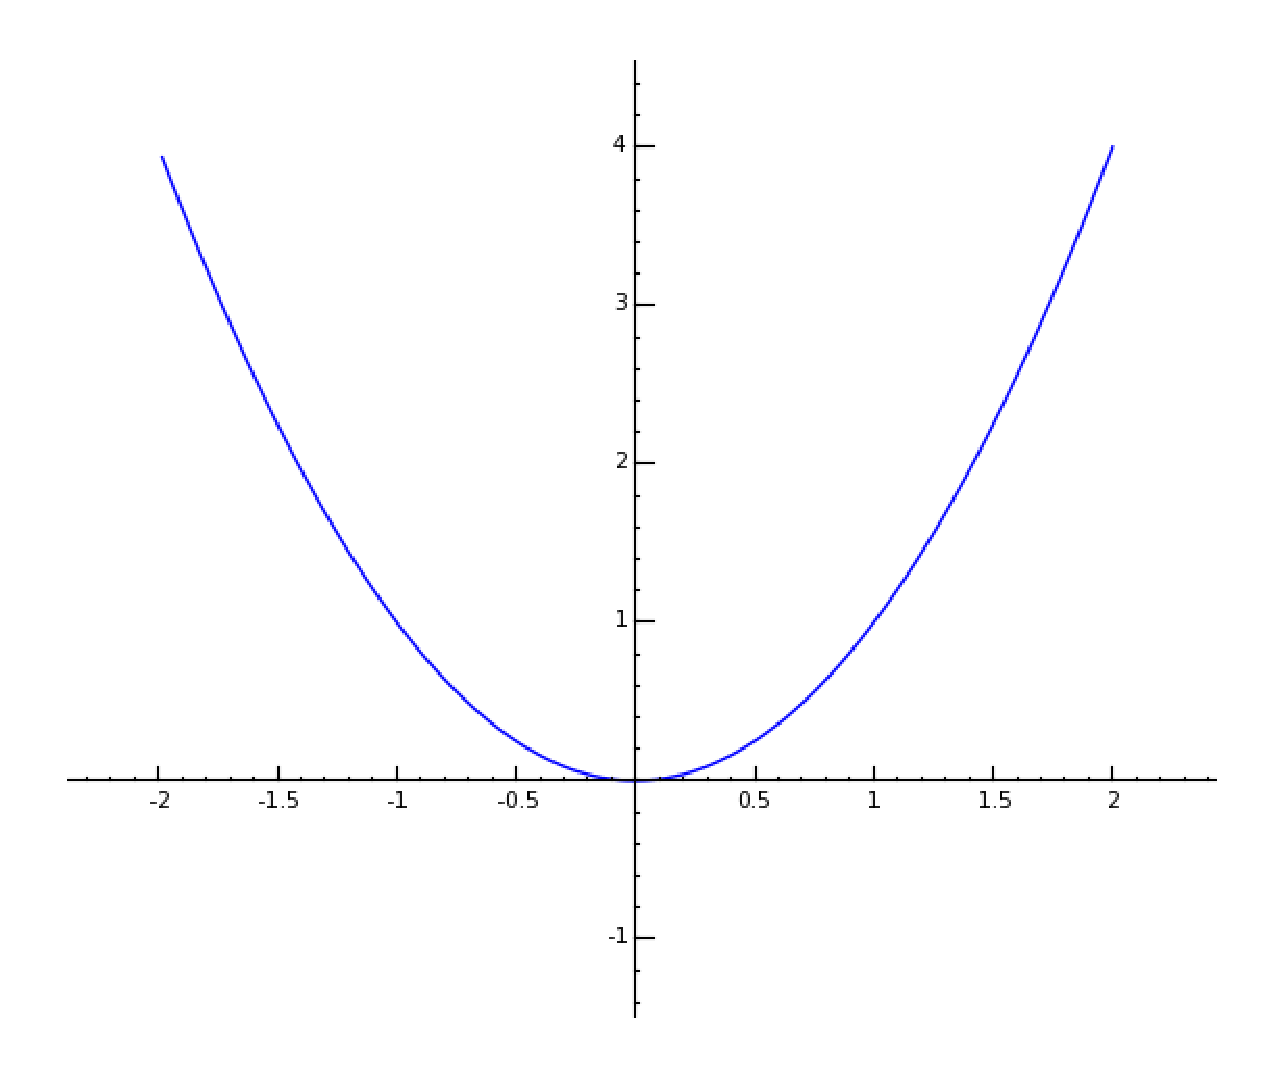
\includegraphics[height=5cm,width=3cm]{parabola.eps}%
\lthtmlpictureZ
\lthtmlcheckvsize\clearpage}

{\newpage\clearpage
\lthtmlinlinemathA{tex2html_wrap_inline44468}%
$ \sin x$%
\lthtmlinlinemathZ
\lthtmlcheckvsize\clearpage}

{\newpage\clearpage
\lthtmlinlinemathA{tex2html_wrap_inline44470}%
$ y = \sin\, x$%
\lthtmlinlinemathZ
\lthtmlcheckvsize\clearpage}

{\newpage\clearpage
\lthtmlpictureA{tex2html_wrap44472}%
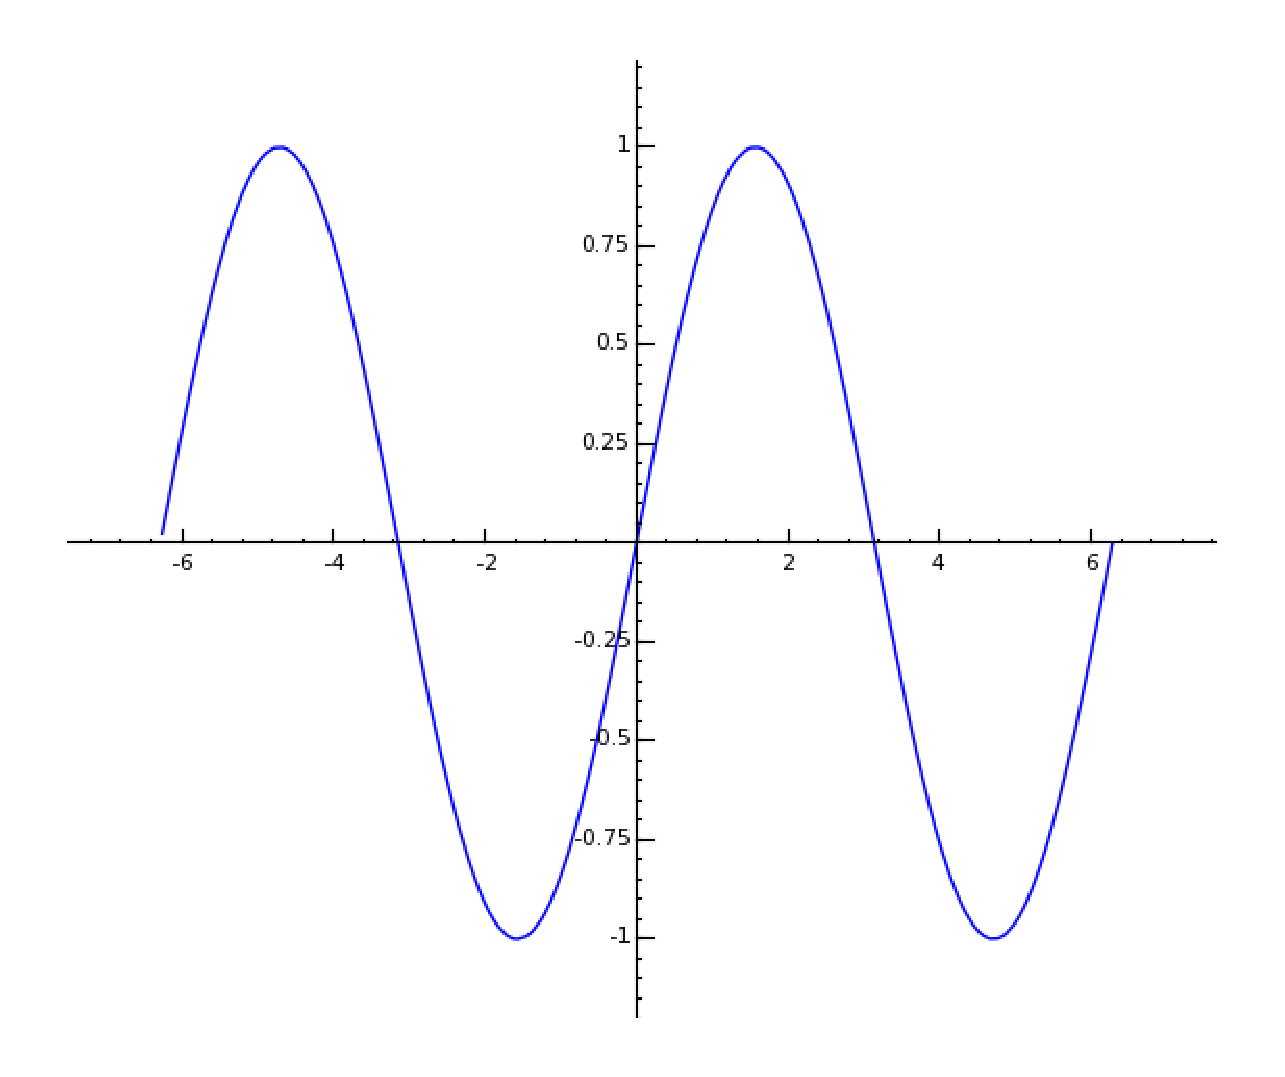
\includegraphics[height=3cm,width=9cm]{sine.eps}%
\lthtmlpictureZ
\lthtmlcheckvsize\clearpage}

{\newpage\clearpage
\lthtmlinlinemathA{tex2html_wrap_inline44477}%
$ exp(x) = e^x$%
\lthtmlinlinemathZ
\lthtmlcheckvsize\clearpage}

{\newpage\clearpage
\lthtmlinlinemathA{tex2html_wrap_indisplay44479}%
$\displaystyle y= e^x, \qquad (e = 2.718\cdots),
$%
\lthtmlindisplaymathZ
\lthtmlcheckvsize\clearpage}

{\newpage\clearpage
\lthtmlpictureA{tex2html_wrap44481}%
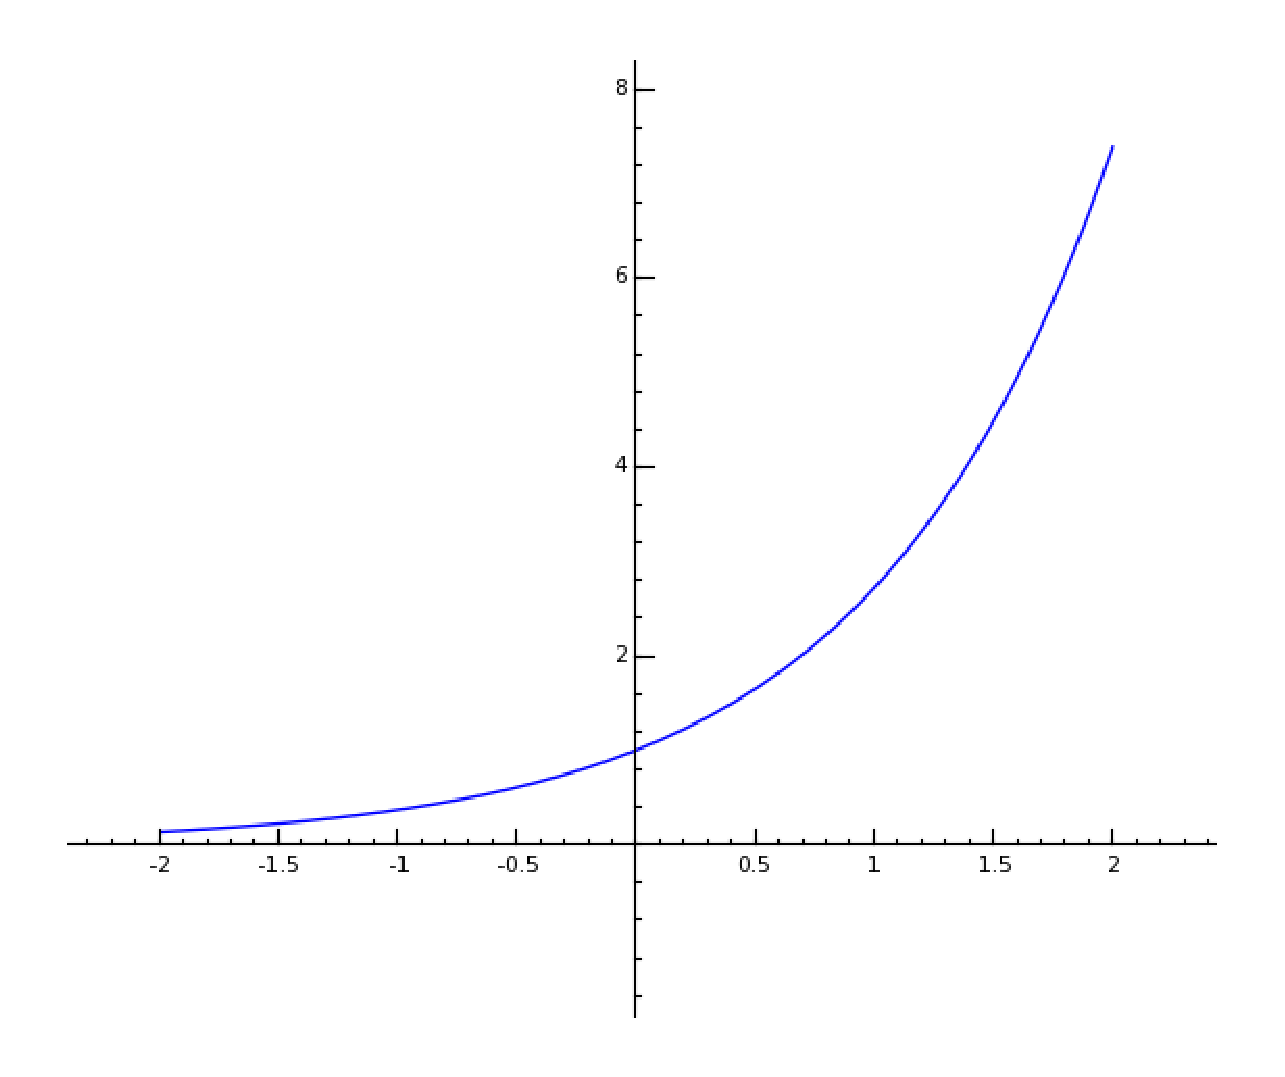
\includegraphics[height=5cm,width=5cm]{exp.eps}%
\lthtmlpictureZ
\lthtmlcheckvsize\clearpage}

{\newpage\clearpage
\lthtmlinlinemathA{tex2html_wrap_inline44489}%
$ x = 0$%
\lthtmlinlinemathZ
\lthtmlcheckvsize\clearpage}

{\newpage\clearpage
\lthtmlinlinemathA{tex2html_wrap_inline44491}%
$ \lim_{x \to 0} y (= \lim_{x \to 0} e^x) = 1$%
\lthtmlinlinemathZ
\lthtmlcheckvsize\clearpage}

{\newpage\clearpage
\lthtmlinlinemathA{tex2html_wrap_inline44493}%
$ x > 0$%
\lthtmlinlinemathZ
\lthtmlcheckvsize\clearpage}

{\newpage\clearpage
\lthtmlinlinemathA{tex2html_wrap_inline44495}%
$ y (= e^x)$%
\lthtmlinlinemathZ
\lthtmlcheckvsize\clearpage}

{\newpage\clearpage
\lthtmlinlinemathA{tex2html_wrap_inline44497}%
$ x < 0$%
\lthtmlinlinemathZ
\lthtmlcheckvsize\clearpage}

{\newpage\clearpage
\lthtmlinlinemathA{tex2html_wrap_inline44504}%
$ \ln \, x = \log_e\  x$%
\lthtmlinlinemathZ
\lthtmlcheckvsize\clearpage}

{\newpage\clearpage
\lthtmlinlinemathA{tex2html_wrap_indisplay44506}%
$\displaystyle y = \log_e\  x,
$%
\lthtmlindisplaymathZ
\lthtmlcheckvsize\clearpage}

{\newpage\clearpage
\lthtmlinlinemathA{tex2html_wrap_inline44508}%
$ OX$%
\lthtmlinlinemathZ
\lthtmlcheckvsize\clearpage}

{\newpage\clearpage
\lthtmlinlinemathA{tex2html_wrap_inline44510}%
$ OY$%
\lthtmlinlinemathZ
\lthtmlcheckvsize\clearpage}

{\newpage\clearpage
\lthtmlpictureA{tex2html_wrap44518}%
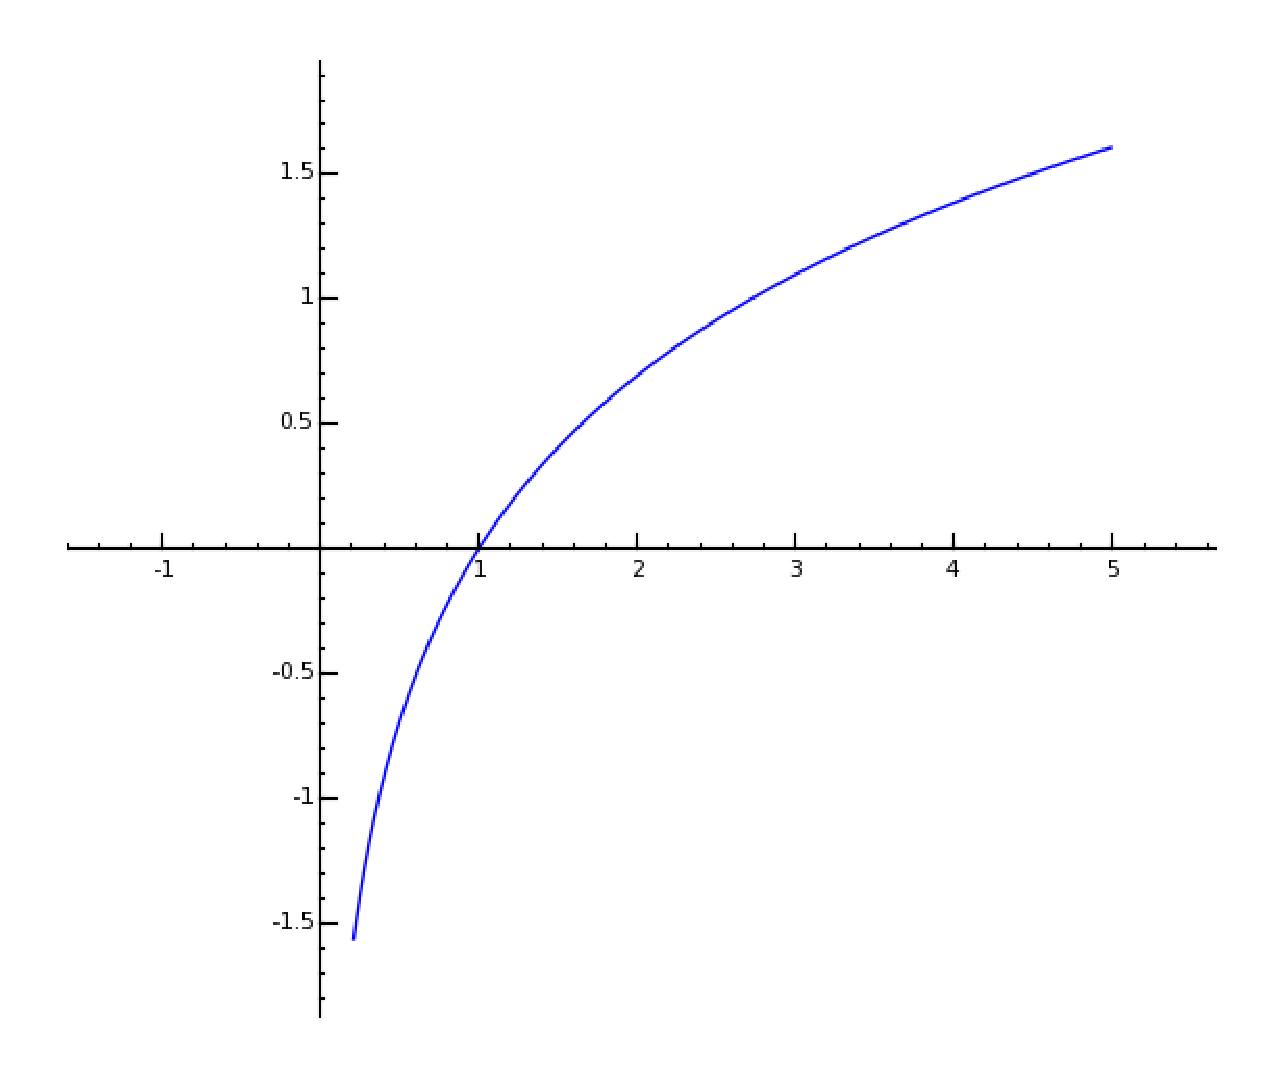
\includegraphics[height=4cm,width=7cm]{ln.eps}%
\lthtmlpictureZ
\lthtmlcheckvsize\clearpage}

{\newpage\clearpage
\lthtmlinlinemathA{tex2html_wrap_inline44529}%
$ \log_e\  x = \log_e\  1 = 0$%
\lthtmlinlinemathZ
\lthtmlcheckvsize\clearpage}

{\newpage\clearpage
\lthtmlinlinemathA{tex2html_wrap_inline44531}%
$ x > 1$%
\lthtmlinlinemathZ
\lthtmlcheckvsize\clearpage}

{\newpage\clearpage
\lthtmlinlinemathA{tex2html_wrap_inline44533}%
$ \log_e\  x$%
\lthtmlinlinemathZ
\lthtmlcheckvsize\clearpage}

{\newpage\clearpage
\lthtmlinlinemathA{tex2html_wrap_inline44537}%
$ 1 > x > 0$%
\lthtmlinlinemathZ
\lthtmlcheckvsize\clearpage}

{\newpage\clearpage
\lthtmlinlinemathA{tex2html_wrap_inline44543}%
$ \lim_{x \to 0} \log\  x = -\infty$%
\lthtmlinlinemathZ
\lthtmlcheckvsize\clearpage}

{\newpage\clearpage
\lthtmlinlinemathA{tex2html_wrap_inline44545}%
$ x \le 0$%
\lthtmlinlinemathZ
\lthtmlcheckvsize\clearpage}

{\newpage\clearpage
\lthtmlinlinemathA{tex2html_wrap_inline44555}%
$ \frac{1}{x}$%
\lthtmlinlinemathZ
\lthtmlcheckvsize\clearpage}

{\newpage\clearpage
\lthtmlinlinemathA{tex2html_wrap_indisplay44557}%
$\displaystyle y = \frac{1}{x}
$%
\lthtmlindisplaymathZ
\lthtmlcheckvsize\clearpage}

{\newpage\clearpage
\lthtmlpictureA{tex2html_wrap44562}%
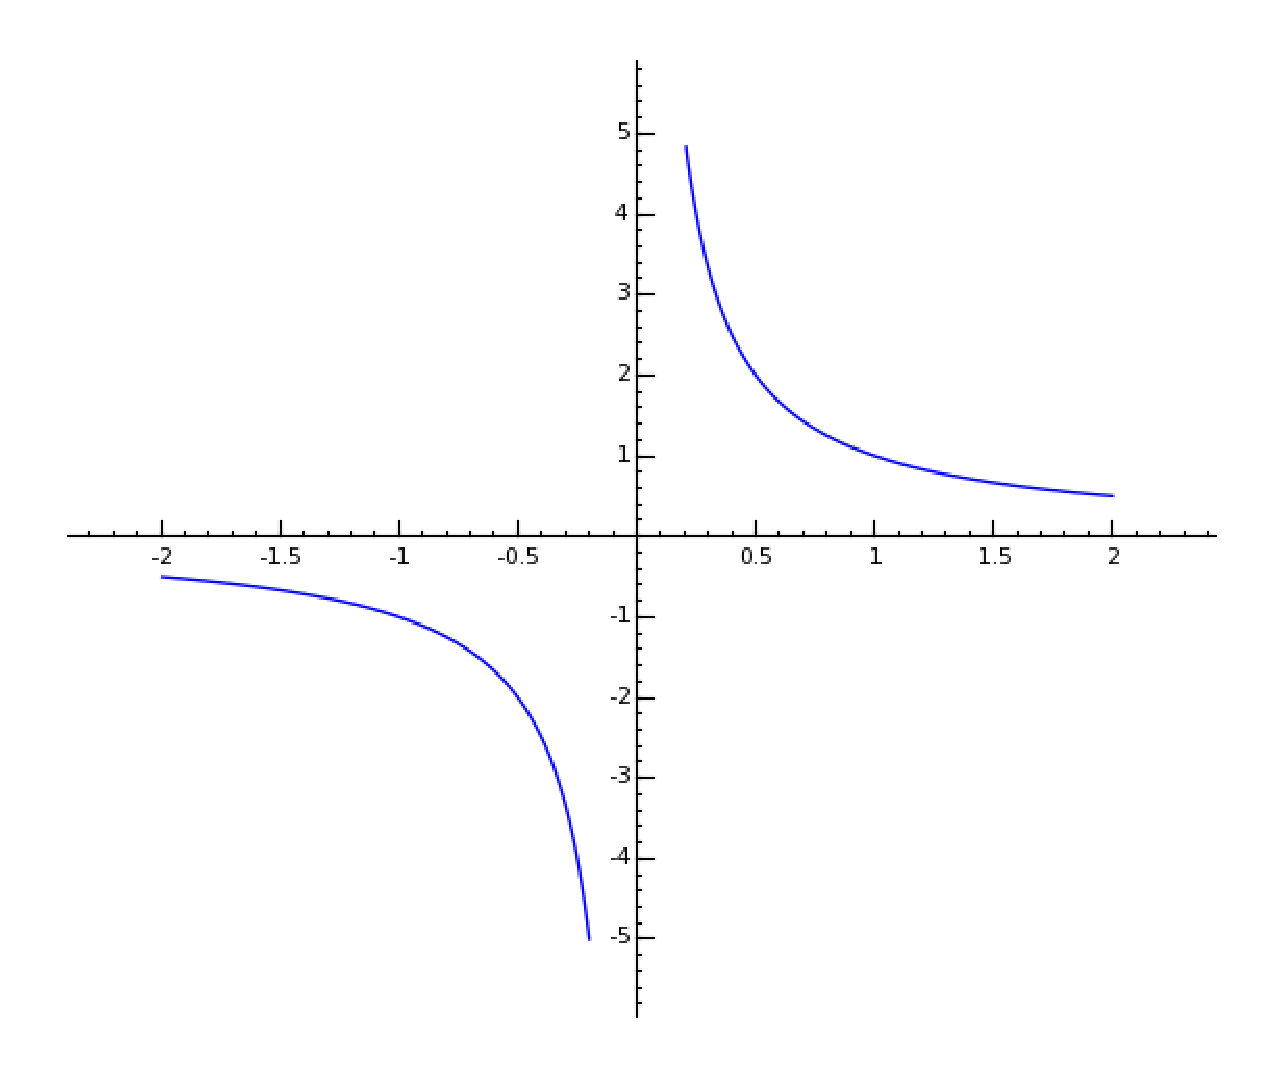
\includegraphics[height=5cm,width=7cm]{recip.eps}%
\lthtmlpictureZ
\lthtmlcheckvsize\clearpage}

{\newpage\clearpage
\lthtmlinlinemathA{tex2html_wrap_indisplay44577}%
$\displaystyle y = \frac{2x}{1 - x^2}
$%
\lthtmlindisplaymathZ
\lthtmlcheckvsize\clearpage}

{\newpage\clearpage
\lthtmlinlinemathA{tex2html_wrap_inline44579}%
$ \frac{2x}{1 - x^2}$%
\lthtmlinlinemathZ
\lthtmlcheckvsize\clearpage}

{\newpage\clearpage
\lthtmlinlinemathA{tex2html_wrap_inline44581}%
$ x = \pm 1$%
\lthtmlinlinemathZ
\lthtmlcheckvsize\clearpage}

{\newpage\clearpage
\lthtmlpictureA{tex2html_wrap44584}%
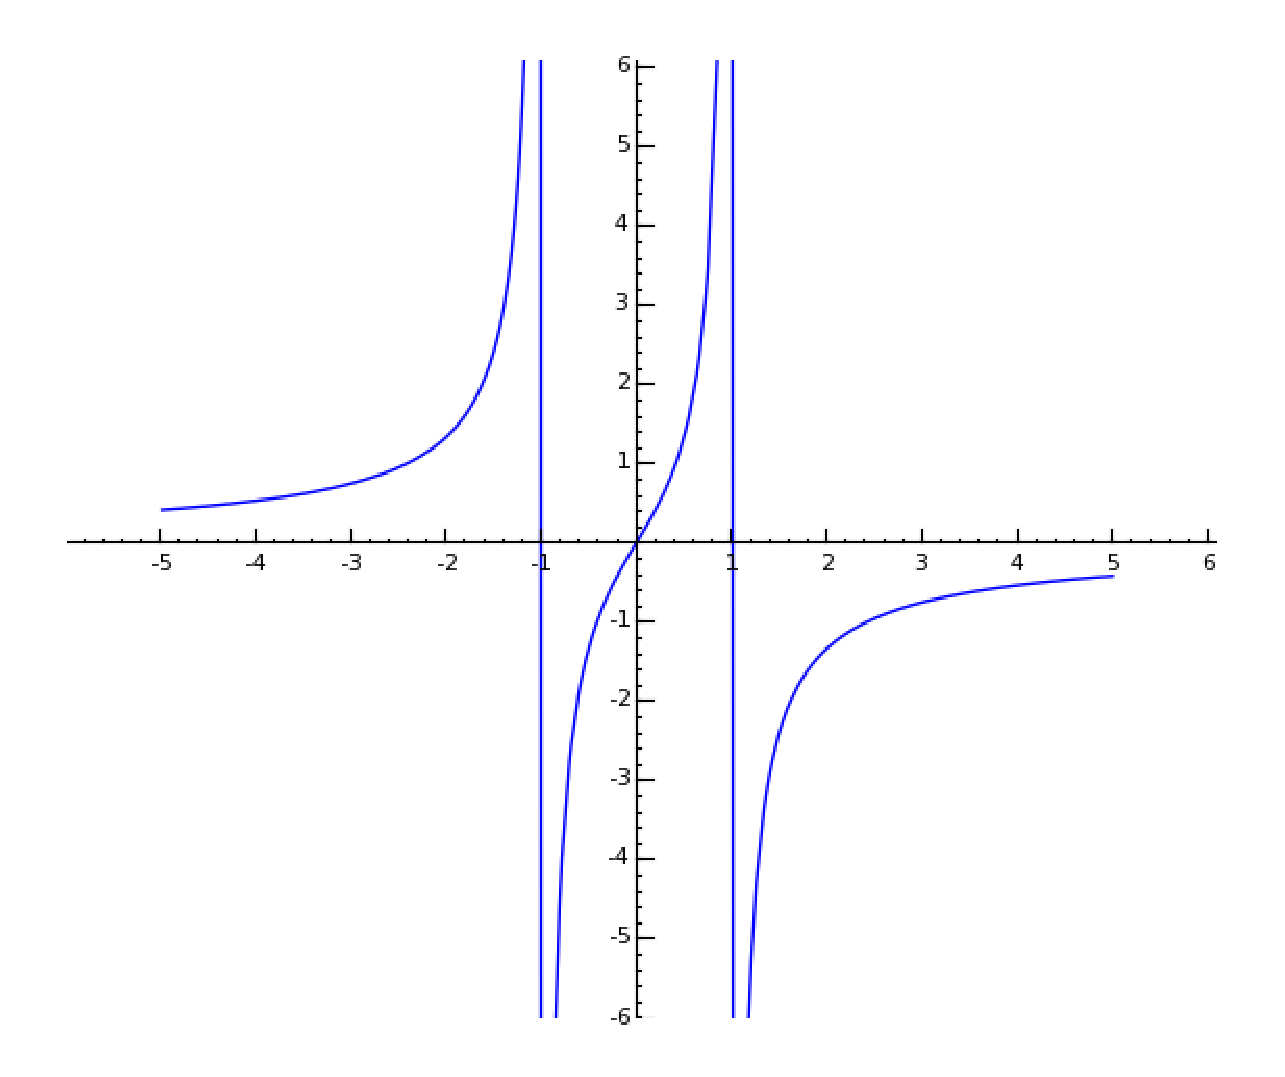
\includegraphics[height=7cm,width=7cm]{fcn6-III.eps}%
\lthtmlpictureZ
\lthtmlcheckvsize\clearpage}

{\newpage\clearpage
\lthtmlinlinemathA{tex2html_wrap_indisplay44593}%
$\displaystyle y = \tan\  x
$%
\lthtmlindisplaymathZ
\lthtmlcheckvsize\clearpage}

{\newpage\clearpage
\lthtmlinlinemathA{tex2html_wrap_inline44595}%
$ \tan x$%
\lthtmlinlinemathZ
\lthtmlcheckvsize\clearpage}

{\newpage\clearpage
\lthtmlinlinemathA{tex2html_wrap_inline44599}%
$ x = \frac{n\pi}{2}$%
\lthtmlinlinemathZ
\lthtmlcheckvsize\clearpage}

{\newpage\clearpage
\lthtmlpictureA{tex2html_wrap44602}%
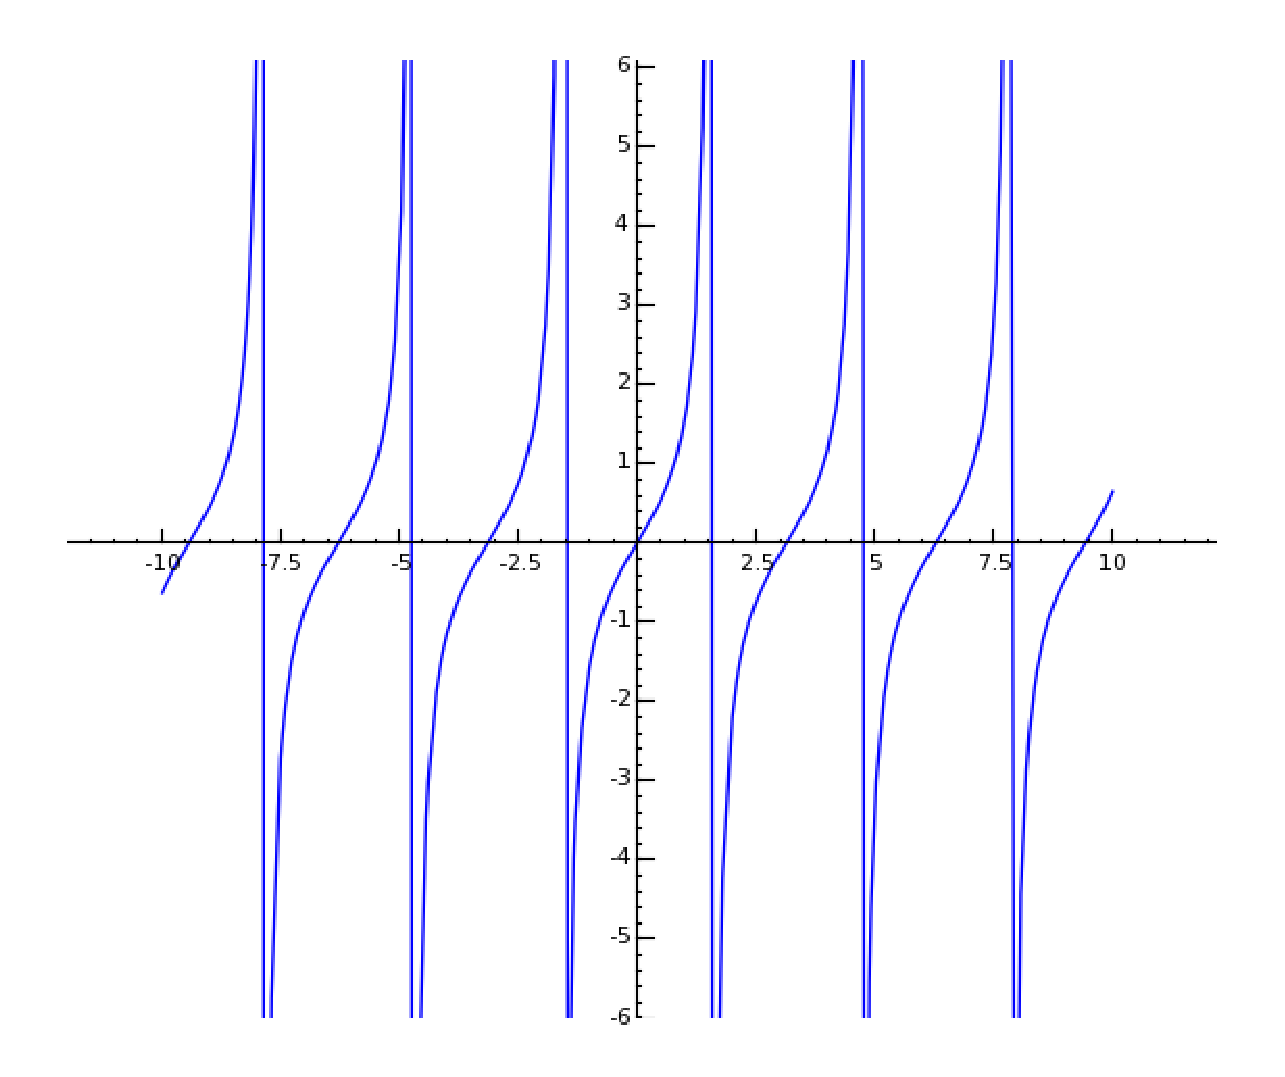
\includegraphics[height=5cm,width=8cm]{tan.eps}%
\lthtmlpictureZ
\lthtmlcheckvsize\clearpage}

{\newpage\clearpage
\lthtmlinlinemathA{tex2html_wrap_inline44607}%
$ \arctan\  x$%
\lthtmlinlinemathZ
\lthtmlcheckvsize\clearpage}

{\newpage\clearpage
\lthtmlinlinemathA{tex2html_wrap_indisplay44611}%
$\displaystyle y = \arctan\  x 
$%
\lthtmlindisplaymathZ
\lthtmlcheckvsize\clearpage}

{\newpage\clearpage
\lthtmlpictureA{tex2html_wrap44612}%
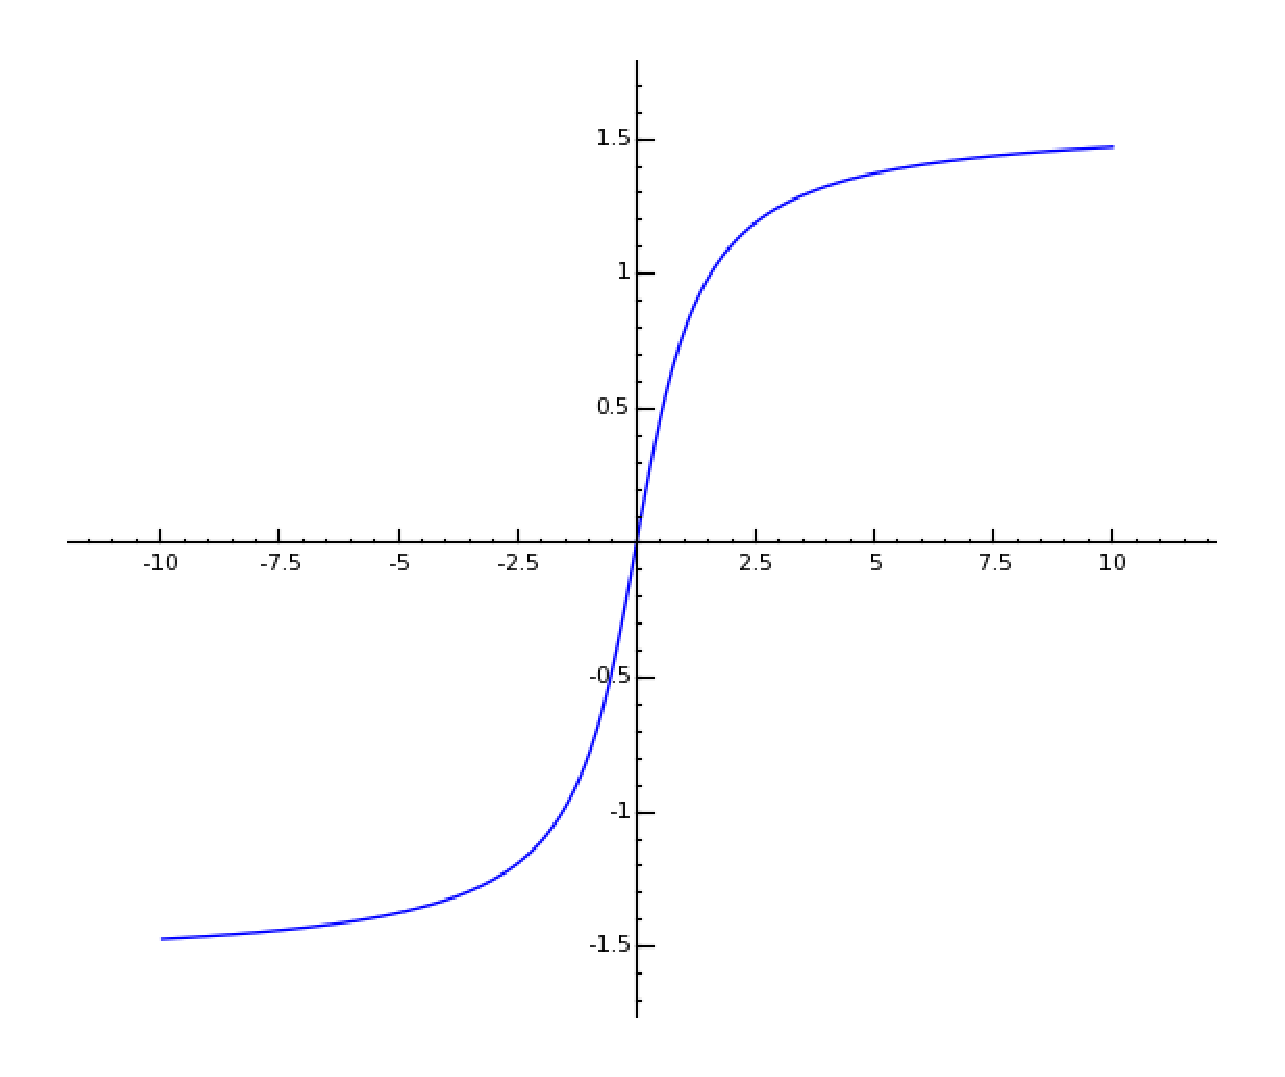
\includegraphics[height=4cm,width=8cm]{arctan.eps}%
\lthtmlpictureZ
\lthtmlcheckvsize\clearpage}

{\newpage\clearpage
\lthtmlinlinemathA{tex2html_wrap_inline44623}%
$ -\frac{\pi}{2}$%
\lthtmlinlinemathZ
\lthtmlcheckvsize\clearpage}

{\newpage\clearpage
\lthtmlinlinemathA{tex2html_wrap_inline44627}%
$ \arctan \frac{1}{x}$%
\lthtmlinlinemathZ
\lthtmlcheckvsize\clearpage}

{\newpage\clearpage
\lthtmlinlinemathA{tex2html_wrap_indisplay44629}%
$\displaystyle y = \arctan\  \frac{1}{x}, 
$%
\lthtmlindisplaymathZ
\lthtmlcheckvsize\clearpage}

{\newpage\clearpage
\lthtmlinlinemathA{tex2html_wrap_inline44641}%
$ +\frac{\pi}{2}$%
\lthtmlinlinemathZ
\lthtmlcheckvsize\clearpage}

{\newpage\clearpage
\lthtmlpictureA{tex2html_wrap44646}%
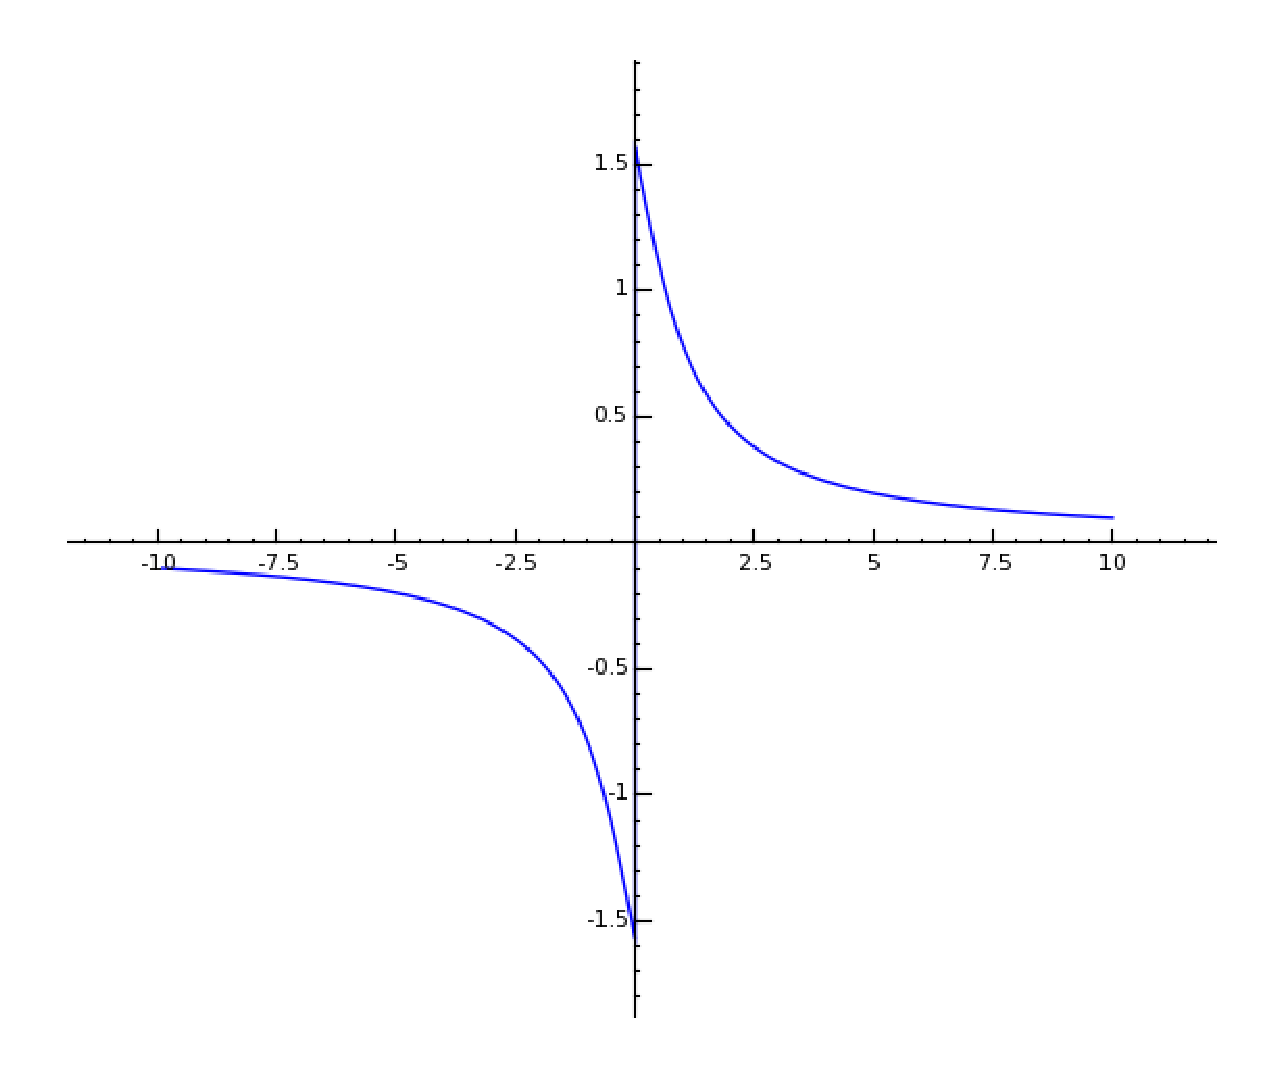
\includegraphics[height=4cm,width=8cm]{arctan1ox.eps}%
\lthtmlpictureZ
\lthtmlcheckvsize\clearpage}

{\newpage\clearpage
\lthtmlinlinemathA{tex2html_wrap_inline44650}%
$ y=\arctan(1/x)$%
\lthtmlinlinemathZ
\lthtmlcheckvsize\clearpage}

{\newpage\clearpage
\lthtmldisplayA{displaymath44655}%
\begin{displaymath}
f(x) = 
\left\{
\begin{array}{ll}
-1, & x<-\pi/2,\\
\sin(x), &\pi/2\leq x\leq \pi/2,\\
1, &\pi/2<x.
\end{array}
\right.
\end{displaymath}%
\lthtmldisplayZ
\lthtmlcheckvsize\clearpage}

{\newpage\clearpage
\lthtmlpictureA{tex2html_wrap44656}%
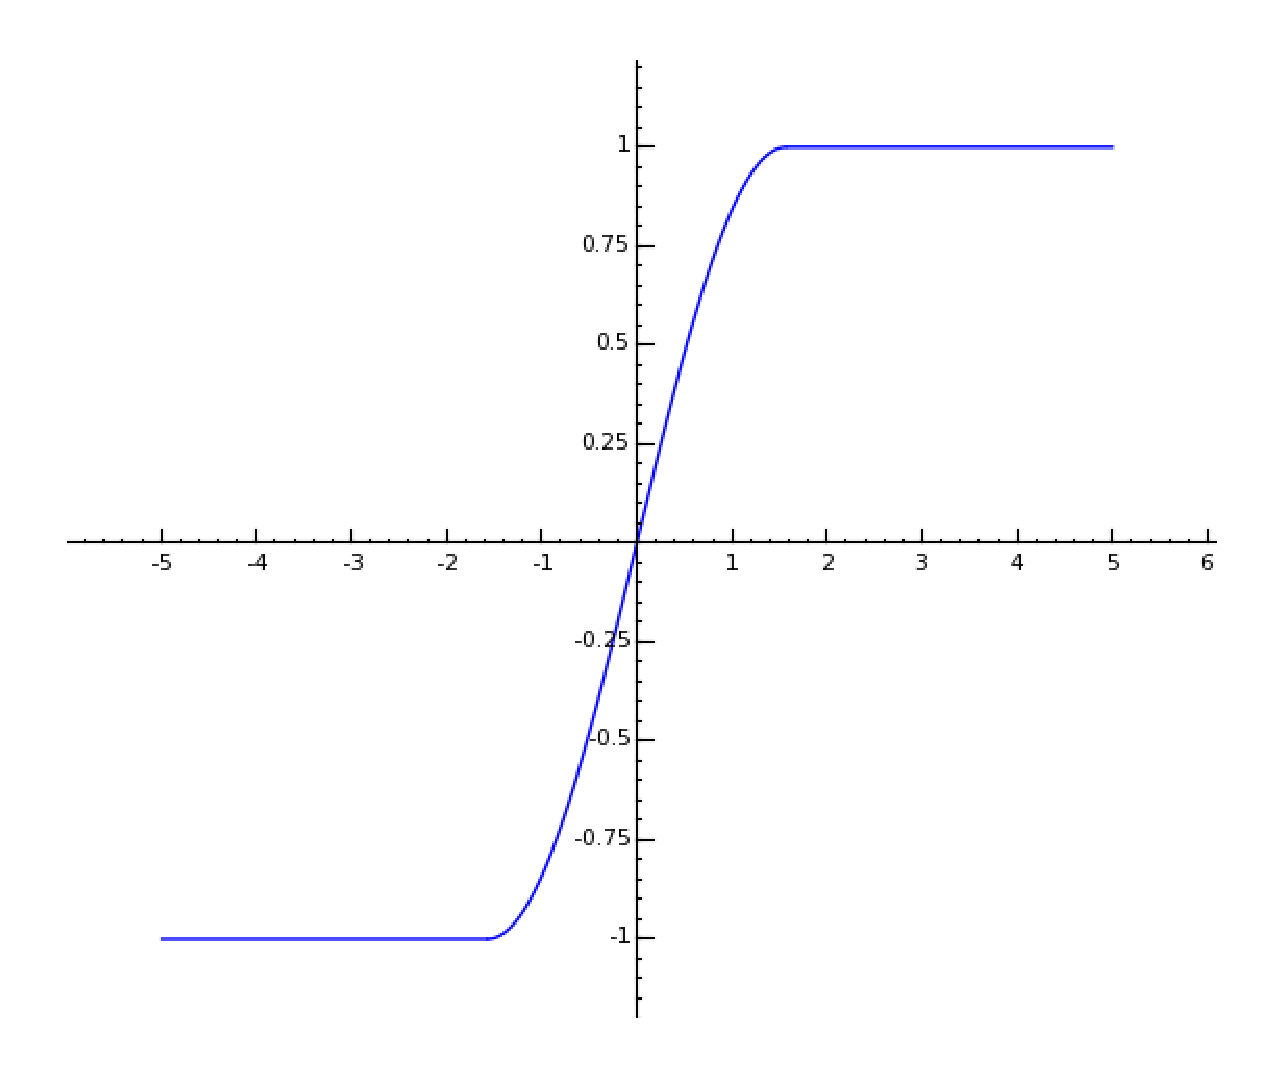
\includegraphics[height=4cm,width=8cm]{piecewise.eps}%
\lthtmlpictureZ
\lthtmlcheckvsize\clearpage}

{\newpage\clearpage
\lthtmldisplayA{displaymath44661}%
\begin{displaymath}
f(x) = 
\left\{
\begin{array}{ll}
-1, & x<-2,\\
3, &-2\leq x\leq 3,\\
2, &3<x.
\end{array}
\right.
\end{displaymath}%
\lthtmldisplayZ
\lthtmlcheckvsize\clearpage}

{\newpage\clearpage
\lthtmlinlinemathA{tex2html_wrap_inline44663}%
$ x=-2$%
\lthtmlinlinemathZ
\lthtmlcheckvsize\clearpage}

{\newpage\clearpage
\lthtmlinlinemathA{tex2html_wrap_inline44665}%
$ x=3$%
\lthtmlinlinemathZ
\lthtmlcheckvsize\clearpage}

{\newpage\clearpage
\lthtmlpictureA{tex2html_wrap44666}%
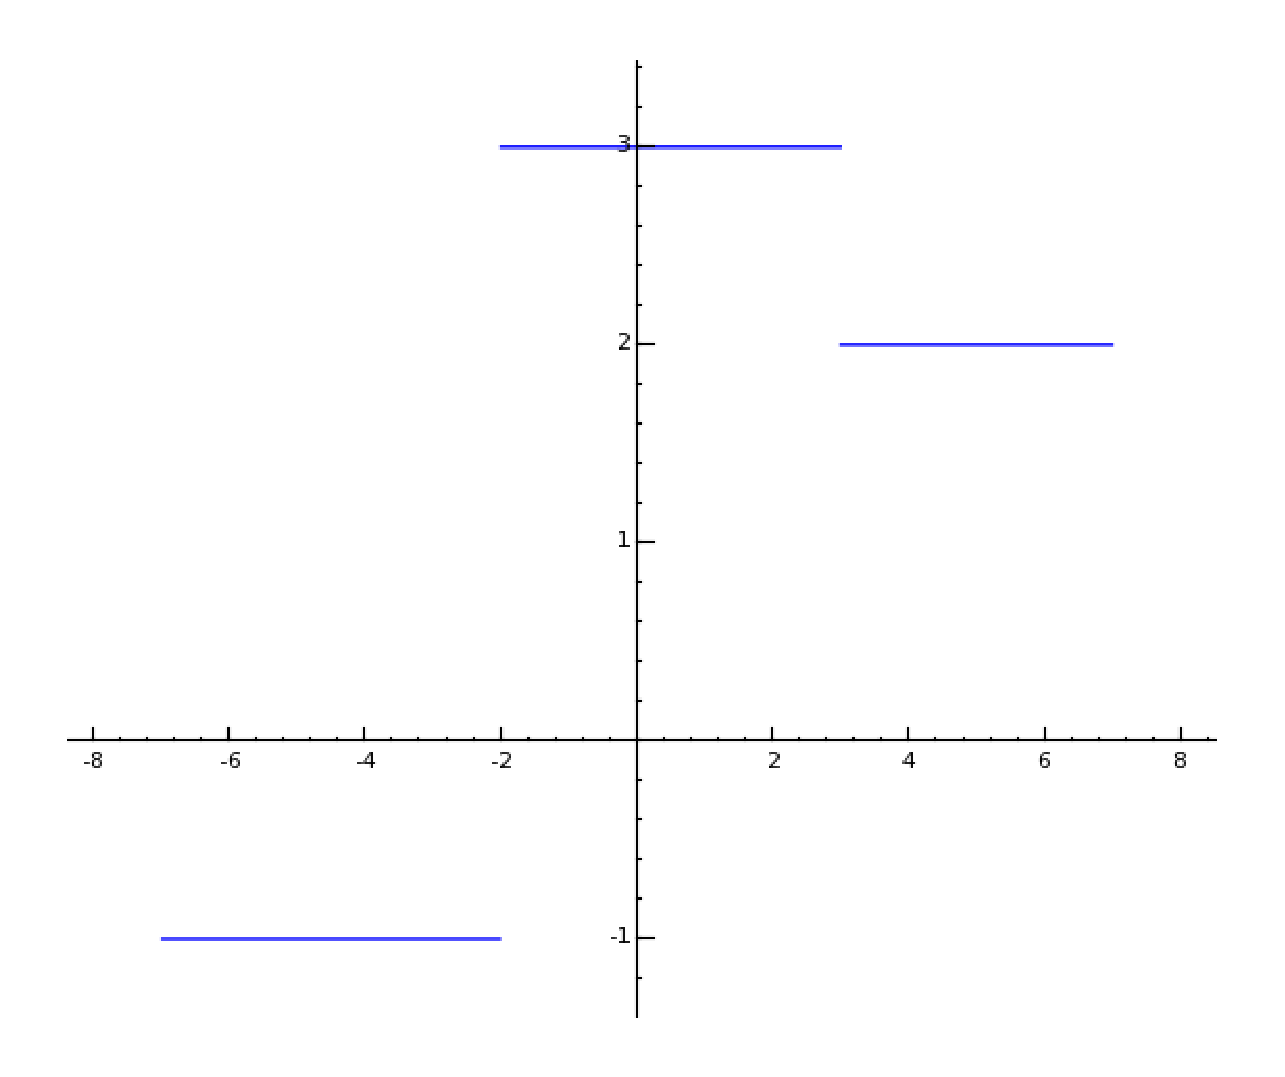
\includegraphics[height=4cm,width=8cm]{piecewise2.eps}%
\lthtmlpictureZ
\lthtmlcheckvsize\clearpage}

\stepcounter{section}
{\newpage\clearpage
\lthtmlinlinemathA{tex2html_wrap_indisplay44677}%
$\displaystyle \lim_{x\to a} [f(x)+g(x)] = \lim_{x\to a} f(x)
+\lim_{x\to a} g(x).
$%
\lthtmlindisplaymathZ
\lthtmlcheckvsize\clearpage}

{\newpage\clearpage
\lthtmlinlinemathA{tex2html_wrap_indisplay44684}%
$\displaystyle \lim_{x\to a} [f(x)\cdot g(x)] = \lim_{x\to a} f(x)
\cdot \lim_{x\to a} g(x).
$%
\lthtmlindisplaymathZ
\lthtmlcheckvsize\clearpage}

{\newpage\clearpage
\lthtmlinlinemathA{tex2html_wrap_indisplay44691}%
$\displaystyle \lim_{x\to a} [f(x)/g(x)] = \frac{\lim_{x\to a} f(x)}{\lim_{x\to a} g(x)},
$%
\lthtmlindisplaymathZ
\lthtmlcheckvsize\clearpage}

{\newpage\clearpage
\lthtmlinlinemathA{tex2html_wrap_inline44693}%
$ \lim_{x\to a} g(x)\not= 0$%
\lthtmlinlinemathZ
\lthtmlcheckvsize\clearpage}

{\newpage\clearpage
\lthtmlinlinemathA{tex2html_wrap_inline44697}%
$ \epsilon$%
\lthtmlinlinemathZ
\lthtmlcheckvsize\clearpage}

{\newpage\clearpage
\lthtmlinlinemathA{tex2html_wrap_inline44699}%
$ \frac{\epsilon}{n}$%
\lthtmlinlinemathZ
\lthtmlcheckvsize\clearpage}

{\newpage\clearpage
\lthtmlinlinemathA{tex2html_wrap_inline44705}%
$ c\not= 0$%
\lthtmlinlinemathZ
\lthtmlcheckvsize\clearpage}

{\newpage\clearpage
\lthtmlinlinemathA{tex2html_wrap_inline44709}%
$ \frac{\epsilon}{|c|}$%
\lthtmlinlinemathZ
\lthtmlcheckvsize\clearpage}

{\newpage\clearpage
\lthtmlinlinemathA{tex2html_wrap_inline44717}%
$ v\to L$%
\lthtmlinlinemathZ
\lthtmlcheckvsize\clearpage}

{\newpage\clearpage
\lthtmlinlinemathA{tex2html_wrap_inline44719}%
$ k$%
\lthtmlinlinemathZ
\lthtmlcheckvsize\clearpage}

{\newpage\clearpage
\lthtmlinlinemathA{tex2html_wrap_inline44727}%
$ \frac{\epsilon}{v}$%
\lthtmlinlinemathZ
\lthtmlcheckvsize\clearpage}

{\newpage\clearpage
\lthtmlinlinemathA{tex2html_wrap_inline44731}%
$ \frac{\epsilon}{k}$%
\lthtmlinlinemathZ
\lthtmlcheckvsize\clearpage}

{\newpage\clearpage
\lthtmlinlinemathA{tex2html_wrap_inline44735}%
$ n-th$%
\lthtmlinlinemathZ
\lthtmlcheckvsize\clearpage}

{\newpage\clearpage
\lthtmlinlinemathA{tex2html_wrap_inline44741}%
$ v_1$%
\lthtmlinlinemathZ
\lthtmlcheckvsize\clearpage}

{\newpage\clearpage
\lthtmlinlinemathA{tex2html_wrap_inline44743}%
$ v_2$%
\lthtmlinlinemathZ
\lthtmlcheckvsize\clearpage}

{\newpage\clearpage
\lthtmlinlinemathA{tex2html_wrap_inline44745}%
$ v_3$%
\lthtmlinlinemathZ
\lthtmlcheckvsize\clearpage}

{\newpage\clearpage
\lthtmlinlinemathA{tex2html_wrap_inline44747}%
$ \dots$%
\lthtmlinlinemathZ
\lthtmlcheckvsize\clearpage}

{\newpage\clearpage
\lthtmlinlinemathA{tex2html_wrap_inline44749}%
$ L_1$%
\lthtmlinlinemathZ
\lthtmlcheckvsize\clearpage}

{\newpage\clearpage
\lthtmlinlinemathA{tex2html_wrap_inline44751}%
$ L_2$%
\lthtmlinlinemathZ
\lthtmlcheckvsize\clearpage}

{\newpage\clearpage
\lthtmlinlinemathA{tex2html_wrap_inline44753}%
$ L_3$%
\lthtmlinlinemathZ
\lthtmlcheckvsize\clearpage}

{\newpage\clearpage
\lthtmlinlinemathA{tex2html_wrap_indisplay44757}%
$\displaystyle v_1 - L_1 	= \epsilon_1,\  \ 
v_2 - L_2 	= \epsilon_2,\  \ 
v_3 - L_3 	= \epsilon_3,
$%
\lthtmlindisplaymathZ
\lthtmlcheckvsize\clearpage}

{\newpage\clearpage
\lthtmlinlinemathA{tex2html_wrap_inline44759}%
$ \epsilon_1$%
\lthtmlinlinemathZ
\lthtmlcheckvsize\clearpage}

{\newpage\clearpage
\lthtmlinlinemathA{tex2html_wrap_inline44761}%
$ \epsilon_2$%
\lthtmlinlinemathZ
\lthtmlcheckvsize\clearpage}

{\newpage\clearpage
\lthtmlinlinemathA{tex2html_wrap_inline44763}%
$ \epsilon_3$%
\lthtmlinlinemathZ
\lthtmlcheckvsize\clearpage}

{\newpage\clearpage
\lthtmlinlinemathA{tex2html_wrap_indisplay44767}%
$\displaystyle (v_1 + v _2 + v_3 + \dots) - (L_1 + L_2 + L_3 + . . .) 
= (\epsilon_1 + \epsilon_2 + \epsilon_3 + \dots).
$%
\lthtmlindisplaymathZ
\lthtmlcheckvsize\clearpage}

{\newpage\clearpage
\lthtmlinlinemathA{tex2html_wrap_indisplay44769}%
$\displaystyle \lim (v_1 + v_2 + v_3 + \dots) 
= L_1 + L_2 + L_3 + \dots,
$%
\lthtmlindisplaymathZ
\lthtmlcheckvsize\clearpage}

{\newpage\clearpage
\lthtmlinlinemathA{tex2html_wrap_indisplay44771}%
$\displaystyle \lim (v_1 + v_2 + v_3 + \dots) 
= \lim v_1 + \lim v_2 + \lim v_3 + \dots,
$%
\lthtmlindisplaymathZ
\lthtmlcheckvsize\clearpage}

{\newpage\clearpage
\lthtmlinlinemathA{tex2html_wrap_inline44773}%
$ \Box$%
\lthtmlinlinemathZ
\lthtmlcheckvsize\clearpage}

{\newpage\clearpage
\lthtmlinlinemathA{tex2html_wrap_indisplay44787}%
$\displaystyle v_1 	= L_1 + \epsilon_1
$%
\lthtmlindisplaymathZ
\lthtmlcheckvsize\clearpage}

{\newpage\clearpage
\lthtmlinlinemathA{tex2html_wrap_inline44789}%
$ v_2 = L_2 + \epsilon_2$%
\lthtmlinlinemathZ
\lthtmlcheckvsize\clearpage}

{\newpage\clearpage
\lthtmldisplayA{displaymath44791}%
\begin{displaymath}
\begin{array}
{ll}
v_1v_2 	&= (L_1 + \epsilon_1)(L_2 + \epsilon_2)\\
&	= L_1L_2 + L_1\epsilon_2 + L_2\epsilon_1 + \epsilon_1\epsilon_2
\end{array}
\end{displaymath}%
\lthtmldisplayZ
\lthtmlcheckvsize\clearpage}

{\newpage\clearpage
\lthtmlinlinemathA{tex2html_wrap_indisplay44793}%
$\displaystyle v_1v_2 - L_1L_2 = L_1\epsilon_2 + L_2\epsilon_1 + \epsilon_1\epsilon_2.
$%
\lthtmlindisplaymathZ
\lthtmlcheckvsize\clearpage}

{\newpage\clearpage
\lthtmlinlinemathA{tex2html_wrap_indisplay44795}%
$\displaystyle \lim (v_1v_2) = L_1L_2 = \lim v_1 \cdot \lim v_2,
$%
\lthtmlindisplaymathZ
\lthtmlcheckvsize\clearpage}

{\newpage\clearpage
\lthtmlinlinemathA{tex2html_wrap_indisplay44799}%
$\displaystyle \frac{v_1}{v_2} = \frac{L_1 + \epsilon_1}{L_2 + \epsilon_2} 
= \frac{L_1}{L_2} + \left ( \frac{L_1 + \epsilon_1}{L_2 + \epsilon_2} 
- \frac{L_1}{L_2} \right ),
$%
\lthtmlindisplaymathZ
\lthtmlcheckvsize\clearpage}

{\newpage\clearpage
\lthtmlinlinemathA{tex2html_wrap_indisplay44801}%
$\displaystyle \frac{v_1}{v_2} - \frac{L_1}{L_2} 
= \frac{L_2 \epsilon_1 - L_1 \epsilon_2}{L_2 (L_2 + \epsilon_2)}.
$%
\lthtmlindisplaymathZ
\lthtmlcheckvsize\clearpage}

{\newpage\clearpage
\lthtmlinlinemathA{tex2html_wrap_inline44803}%
$ L_2 \ne 0$%
\lthtmlinlinemathZ
\lthtmlcheckvsize\clearpage}

{\newpage\clearpage
\lthtmlinlinemathA{tex2html_wrap_indisplay44805}%
$\displaystyle \lim \left ( \frac{v_1}{v_2} \right ) = \frac{L_1}{L_2} 
= \frac{\lim\,v_1}{\lim\,v_2},
$%
\lthtmlindisplaymathZ
\lthtmlcheckvsize\clearpage}

\stepcounter{section}
{\newpage\clearpage
\lthtmlinlinemathA{tex2html_wrap_inline44810}%
$ a > 0$%
\lthtmlinlinemathZ
\lthtmlcheckvsize\clearpage}

{\newpage\clearpage
\lthtmlinlinemathA{tex2html_wrap_inline44812}%
$ c \ne 0$%
\lthtmlinlinemathZ
\lthtmlcheckvsize\clearpage}

{\newpage\clearpage
\lthtmlinlinemathA{tex2html_wrap_inline44814}%
$ \lim_{x \to 0} \frac{c}{x} 	= \infty$%
\lthtmlinlinemathZ
\lthtmlcheckvsize\clearpage}

{\newpage\clearpage
\lthtmlinlinemathA{tex2html_wrap_inline44816}%
$ \frac{c}{0} 	= \infty$%
\lthtmlinlinemathZ
\lthtmlcheckvsize\clearpage}

{\newpage\clearpage
\lthtmlinlinemathA{tex2html_wrap_inline44818}%
$ \lim_{x \to \infty} cx 	= \infty$%
\lthtmlinlinemathZ
\lthtmlcheckvsize\clearpage}

{\newpage\clearpage
\lthtmlinlinemathA{tex2html_wrap_inline44820}%
$ c \cdot \infty 	= \infty$%
\lthtmlinlinemathZ
\lthtmlcheckvsize\clearpage}

{\newpage\clearpage
\lthtmlinlinemathA{tex2html_wrap_inline44822}%
$ \lim_{x \to \infty} \frac{x}{c} 	= \infty$%
\lthtmlinlinemathZ
\lthtmlcheckvsize\clearpage}

{\newpage\clearpage
\lthtmlinlinemathA{tex2html_wrap_inline44824}%
$ \frac{\infty}{c} 	= \infty$%
\lthtmlinlinemathZ
\lthtmlcheckvsize\clearpage}

{\newpage\clearpage
\lthtmlinlinemathA{tex2html_wrap_inline44826}%
$ \lim_{x \to \infty} \frac{c}{x} 	= 0$%
\lthtmlinlinemathZ
\lthtmlcheckvsize\clearpage}

{\newpage\clearpage
\lthtmlinlinemathA{tex2html_wrap_inline44828}%
$ \frac{c}{\infty} 	= 0$%
\lthtmlinlinemathZ
\lthtmlcheckvsize\clearpage}

{\newpage\clearpage
\lthtmlinlinemathA{tex2html_wrap_inline44830}%
$ \lim_{x \to -\infty} a^x, 	= +\infty$%
\lthtmlinlinemathZ
\lthtmlcheckvsize\clearpage}

{\newpage\clearpage
\lthtmlinlinemathA{tex2html_wrap_inline44832}%
$ a < 1$%
\lthtmlinlinemathZ
\lthtmlcheckvsize\clearpage}

{\newpage\clearpage
\lthtmlinlinemathA{tex2html_wrap_inline44834}%
$ a^{-\infty} 	= +\infty$%
\lthtmlinlinemathZ
\lthtmlcheckvsize\clearpage}

{\newpage\clearpage
\lthtmlinlinemathA{tex2html_wrap_inline44836}%
$ \lim_{x \to +\infty} a^x 	= 0$%
\lthtmlinlinemathZ
\lthtmlcheckvsize\clearpage}

{\newpage\clearpage
\lthtmlinlinemathA{tex2html_wrap_inline44840}%
$ a^{+\infty} 	= 0$%
\lthtmlinlinemathZ
\lthtmlcheckvsize\clearpage}

{\newpage\clearpage
\lthtmlinlinemathA{tex2html_wrap_inline44842}%
$ \lim_{x \to -\infty} a^x 	= 0$%
\lthtmlinlinemathZ
\lthtmlcheckvsize\clearpage}

{\newpage\clearpage
\lthtmlinlinemathA{tex2html_wrap_inline44844}%
$ a > 1$%
\lthtmlinlinemathZ
\lthtmlcheckvsize\clearpage}

{\newpage\clearpage
\lthtmlinlinemathA{tex2html_wrap_inline44846}%
$ a^{-\infty} 	= 0$%
\lthtmlinlinemathZ
\lthtmlcheckvsize\clearpage}

{\newpage\clearpage
\lthtmlinlinemathA{tex2html_wrap_inline44848}%
$ \lim_{x \to +\infty} a^x 	= +\infty$%
\lthtmlinlinemathZ
\lthtmlcheckvsize\clearpage}

{\newpage\clearpage
\lthtmlinlinemathA{tex2html_wrap_inline44852}%
$ a^{+\infty} 	= +\infty$%
\lthtmlinlinemathZ
\lthtmlcheckvsize\clearpage}

{\newpage\clearpage
\lthtmlinlinemathA{tex2html_wrap_inline44854}%
$ \lim_{x \to 0} \log_a\  x 	= +\infty$%
\lthtmlinlinemathZ
\lthtmlcheckvsize\clearpage}

{\newpage\clearpage
\lthtmlinlinemathA{tex2html_wrap_inline44858}%
$ \log_a\  0 	= +\infty$%
\lthtmlinlinemathZ
\lthtmlcheckvsize\clearpage}

{\newpage\clearpage
\lthtmlinlinemathA{tex2html_wrap_inline44860}%
$ \lim_{x \to +\infty} \log_a\  x 	= -\infty$%
\lthtmlinlinemathZ
\lthtmlcheckvsize\clearpage}

{\newpage\clearpage
\lthtmlinlinemathA{tex2html_wrap_inline44864}%
$ \log_a(+\infty) 	= -\infty$%
\lthtmlinlinemathZ
\lthtmlcheckvsize\clearpage}

{\newpage\clearpage
\lthtmlinlinemathA{tex2html_wrap_inline44866}%
$ \lim_{x \to 0} \log_a\  x 	= -\infty$%
\lthtmlinlinemathZ
\lthtmlcheckvsize\clearpage}

{\newpage\clearpage
\lthtmlinlinemathA{tex2html_wrap_inline44870}%
$ \log_a\  0 	= -\infty$%
\lthtmlinlinemathZ
\lthtmlcheckvsize\clearpage}

{\newpage\clearpage
\lthtmlinlinemathA{tex2html_wrap_inline44872}%
$ \lim_{x \to +\infty} \log_a\  x 	= +\infty$%
\lthtmlinlinemathZ
\lthtmlcheckvsize\clearpage}

{\newpage\clearpage
\lthtmlinlinemathA{tex2html_wrap_inline44876}%
$ \log_a(+\infty) 	= +\infty$%
\lthtmlinlinemathZ
\lthtmlcheckvsize\clearpage}

\stepcounter{section}
{\newpage\clearpage
\lthtmlinlinemathA{tex2html_wrap_inline44953}%
$ \lim_{x \to 0} \frac{\sin\, x}{x} = 1$%
\lthtmlinlinemathZ
\lthtmlcheckvsize\clearpage}

{\newpage\clearpage
\lthtmlinlinemathA{tex2html_wrap_inline44955}%
$ \frac{\sin\, x}{x}$%
\lthtmlinlinemathZ
\lthtmlcheckvsize\clearpage}

{\newpage\clearpage
\lthtmlinlinemathA{tex2html_wrap_inline44962}%
$ \frac{\sin(x)}{x}$%
\lthtmlinlinemathZ
\lthtmlcheckvsize\clearpage}

{\newpage\clearpage
\lthtmlinlinemathA{tex2html_wrap_inline44976}%
$ 10^o$%
\lthtmlinlinemathZ
\lthtmlcheckvsize\clearpage}

{\newpage\clearpage
\lthtmlinlinemathA{tex2html_wrap_inline44982}%
$ \operatorname{arc}\  AM = \operatorname{arc}\  AM' = x$%
\lthtmlinlinemathZ
\lthtmlcheckvsize\clearpage}

{\newpage\clearpage
\lthtmlinlinemathA{tex2html_wrap_inline44984}%
$ MT$%
\lthtmlinlinemathZ
\lthtmlcheckvsize\clearpage}

{\newpage\clearpage
\lthtmlinlinemathA{tex2html_wrap_inline44986}%
$ M'T$%
\lthtmlinlinemathZ
\lthtmlcheckvsize\clearpage}

{\newpage\clearpage
\lthtmlinlinemathA{tex2html_wrap_inline44988}%
$ M$%
\lthtmlinlinemathZ
\lthtmlcheckvsize\clearpage}

{\newpage\clearpage
\lthtmlinlinemathA{tex2html_wrap_inline44990}%
$ M'$%
\lthtmlinlinemathZ
\lthtmlcheckvsize\clearpage}

{\newpage\clearpage
\lthtmlpictureA{tex2html_wrap44992}%
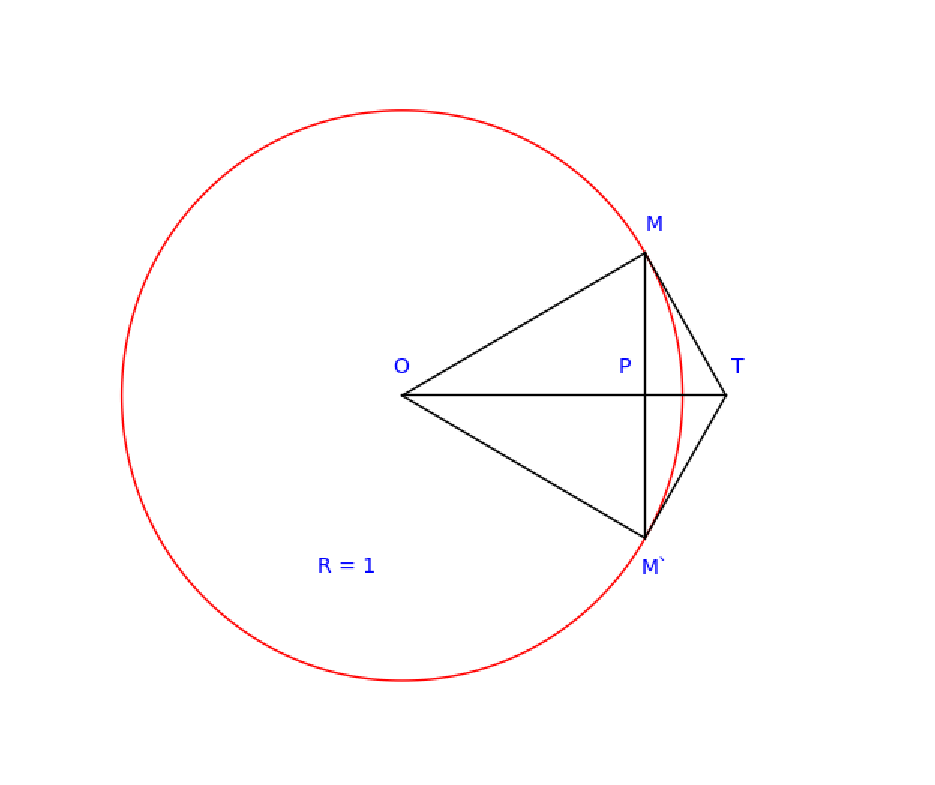
\includegraphics[height=5cm,width=6cm]{circle-tangent.eps}%
\lthtmlpictureZ
\lthtmlcheckvsize\clearpage}

{\newpage\clearpage
\lthtmlinlinemathA{tex2html_wrap_indisplay45005}%
$\displaystyle MPM' < MAM' < MTM';
$%
\lthtmlindisplaymathZ
\lthtmlcheckvsize\clearpage}

{\newpage\clearpage
\lthtmlinlinemathA{tex2html_wrap_inline45007}%
$ 2 \sin\, x < 2x < 2 \tan\  x$%
\lthtmlinlinemathZ
\lthtmlcheckvsize\clearpage}

{\newpage\clearpage
\lthtmlinlinemathA{tex2html_wrap_inline45009}%
$ 2 \sin\, x$%
\lthtmlinlinemathZ
\lthtmlcheckvsize\clearpage}

{\newpage\clearpage
\lthtmlinlinemathA{tex2html_wrap_indisplay45011}%
$\displaystyle 1 < \frac{x}{\sin\, x} < \frac{1}{\cos\  x}.
$%
\lthtmlindisplaymathZ
\lthtmlcheckvsize\clearpage}

{\newpage\clearpage
\lthtmlinlinemathA{tex2html_wrap_indisplay45015}%
$\displaystyle \lim_{x \to 0} \frac{x}{\sin\, x}
$%
\lthtmlindisplaymathZ
\lthtmlcheckvsize\clearpage}

{\newpage\clearpage
\lthtmlinlinemathA{tex2html_wrap_inline45019}%
$ \lim_{x \to 0} \frac{1}{\cos\  x}$%
\lthtmlinlinemathZ
\lthtmlcheckvsize\clearpage}

{\newpage\clearpage
\lthtmlinlinemathA{tex2html_wrap_inline45023}%
$ \lim_{x \to 0} \frac{x}{\sin\, x} = 1$%
\lthtmlinlinemathZ
\lthtmlcheckvsize\clearpage}

{\newpage\clearpage
\lthtmlinlinemathA{tex2html_wrap_indisplay45029}%
$\displaystyle y = \frac{\sin\, x}{x}
$%
\lthtmlindisplaymathZ
\lthtmlcheckvsize\clearpage}

{\newpage\clearpage
\lthtmlpictureA{tex2html_wrap45031}%
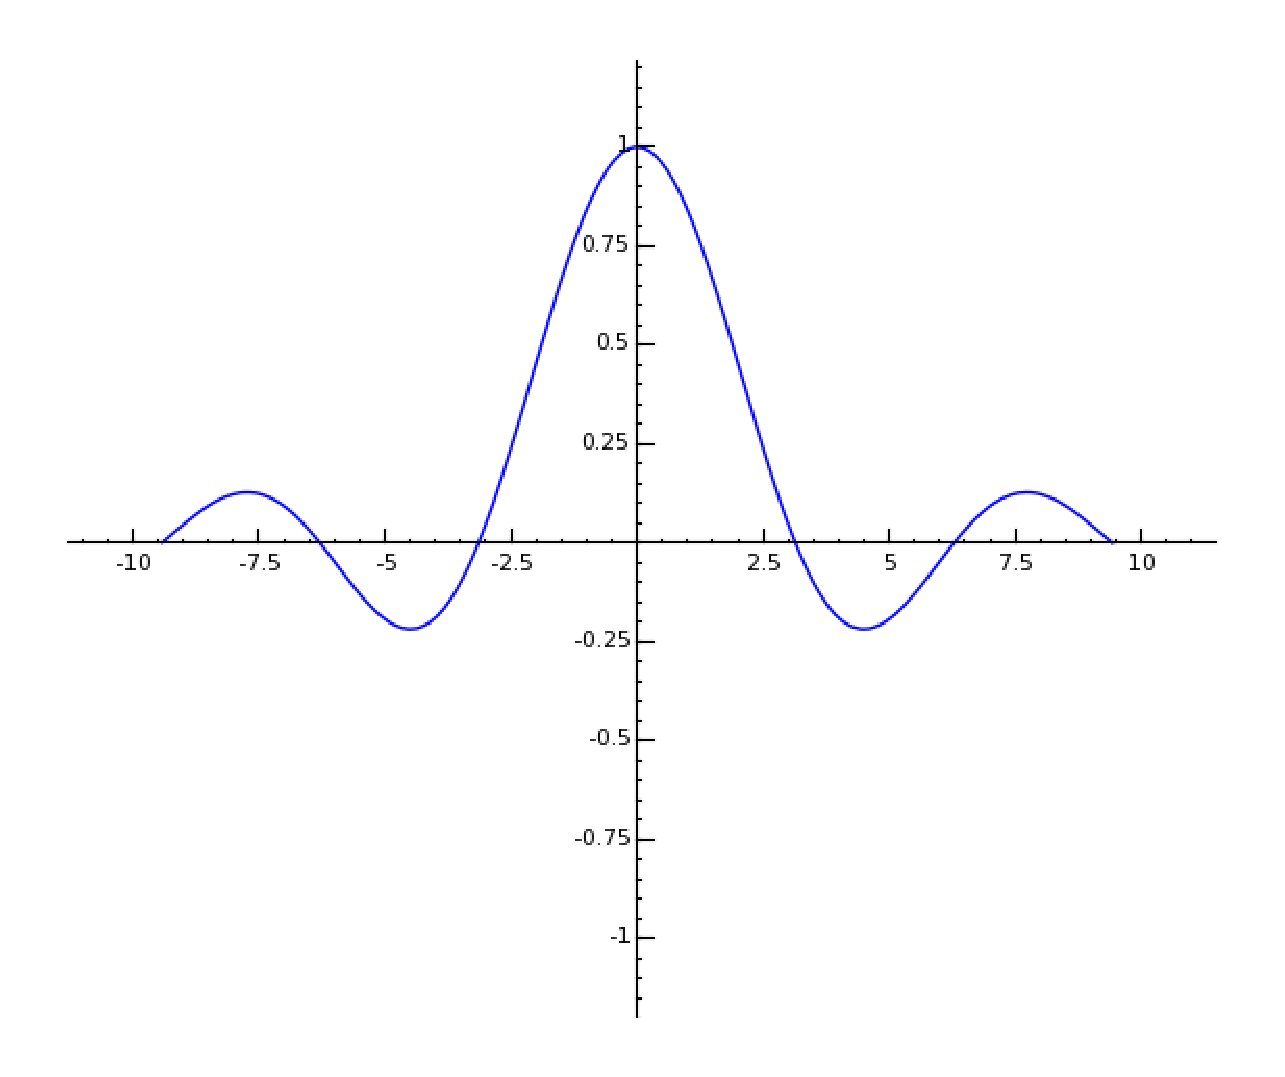
\includegraphics[height=4cm,width=8cm]{limit_proof2.eps}%
\lthtmlpictureZ
\lthtmlcheckvsize\clearpage}

{\newpage\clearpage
\lthtmlinlinemathA{tex2html_wrap_inline45044}%
$ \frac{\sin\, 0}{0} = 1$%
\lthtmlinlinemathZ
\lthtmlcheckvsize\clearpage}

\stepcounter{section}
{\newpage\clearpage
\lthtmlinlinemathA{tex2html_wrap_indisplay45051}%
$\displaystyle \lim_{x \to 0} (1 + x)^{\frac{1}{x}} = 2.71828\cdots = e
$%
\lthtmlindisplaymathZ
\lthtmlcheckvsize\clearpage}

{\newpage\clearpage
\lthtmlinlinemathA{tex2html_wrap_indisplay45055}%
$\displaystyle y = (1 + x)^{\frac{1}{x}}
$%
\lthtmlindisplaymathZ
\lthtmlcheckvsize\clearpage}

{\newpage\clearpage
\lthtmlinlinemathA{tex2html_wrap_inline45057}%
$ x \dot= 0$%
\lthtmlinlinemathZ
\lthtmlcheckvsize\clearpage}

{\newpage\clearpage
\lthtmlinlinemathA{tex2html_wrap_inline45059}%
$ (1 + x)^\frac{1}{x}(= y)$%
\lthtmlinlinemathZ
\lthtmlcheckvsize\clearpage}

{\newpage\clearpage
\lthtmlinlinemathA{tex2html_wrap_inline45061}%
$ 2.718\dots$%
\lthtmlinlinemathZ
\lthtmlcheckvsize\clearpage}

{\newpage\clearpage
\lthtmlinlinemathA{tex2html_wrap_inline45063}%
$ e = 2.718\dots$%
\lthtmlinlinemathZ
\lthtmlcheckvsize\clearpage}

{\newpage\clearpage
\lthtmlpictureA{tex2html_wrap45065}%
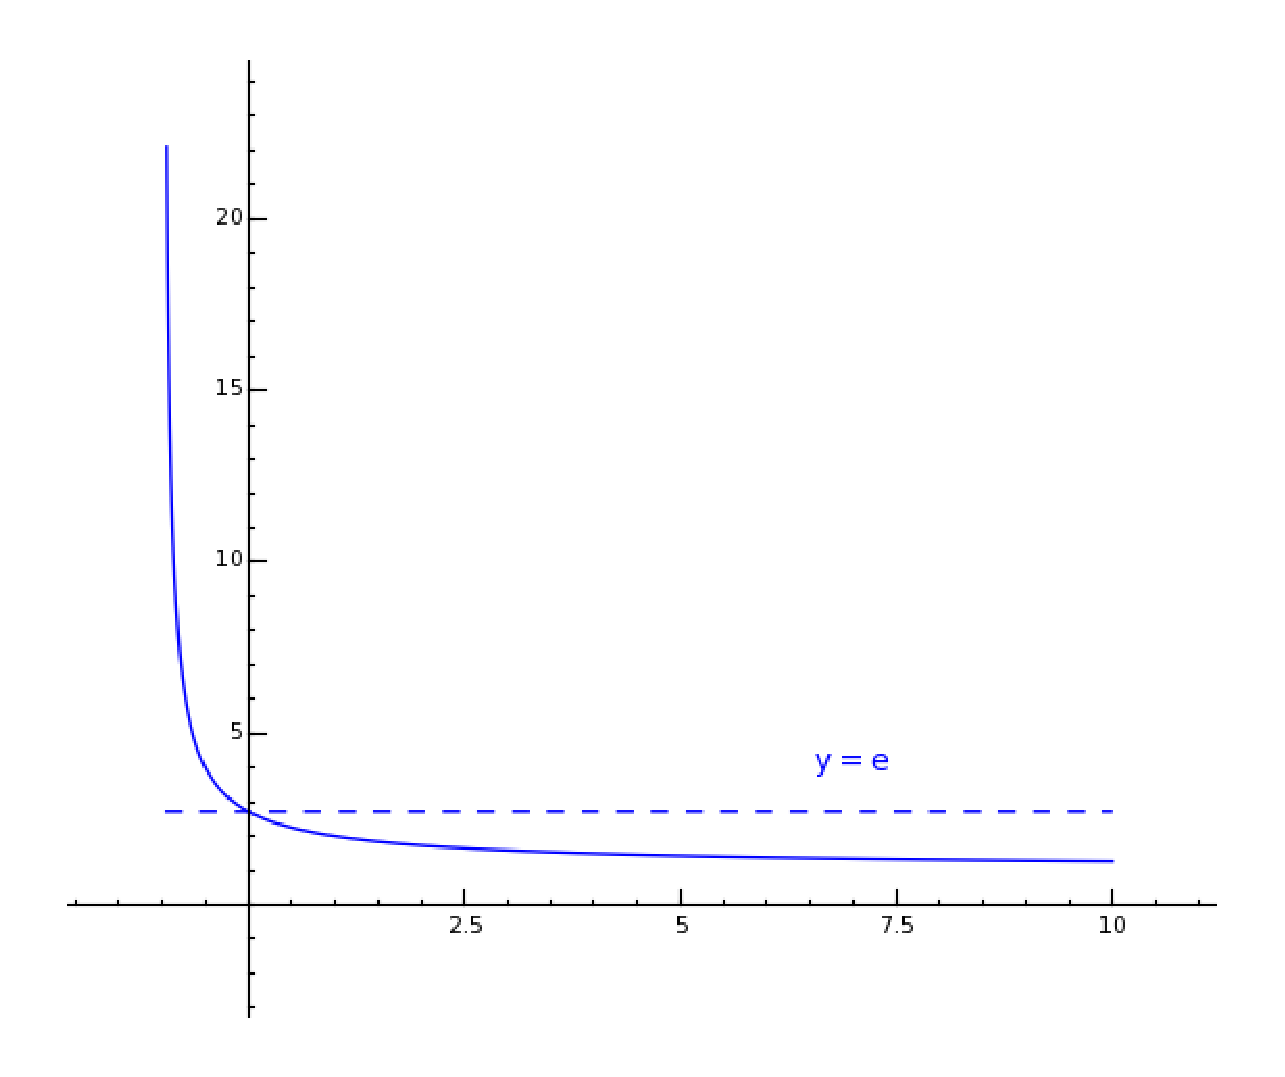
\includegraphics[height=4cm,width=8cm]{limite.eps}%
\lthtmlpictureZ
\lthtmlcheckvsize\clearpage}

{\newpage\clearpage
\lthtmlinlinemathA{tex2html_wrap_inline45076}%
$ y=(1+x)^{1/x}$%
\lthtmlinlinemathZ
\lthtmlcheckvsize\clearpage}

{\newpage\clearpage
\lthtmlinlinemathA{tex2html_wrap_inline45100}%
$ x \to 0-$%
\lthtmlinlinemathZ
\lthtmlcheckvsize\clearpage}

{\newpage\clearpage
\lthtmlinlinemathA{tex2html_wrap_inline45106}%
$ x \to 0+$%
\lthtmlinlinemathZ
\lthtmlcheckvsize\clearpage}

{\newpage\clearpage
\lthtmlinlinemathA{tex2html_wrap_inline45112}%
$ x \to \infty$%
\lthtmlinlinemathZ
\lthtmlcheckvsize\clearpage}

{\newpage\clearpage
\lthtmlinlinemathA{tex2html_wrap_inline45118}%
$ x \to -1+$%
\lthtmlinlinemathZ
\lthtmlcheckvsize\clearpage}

{\newpage\clearpage
\lthtmlinlinemathA{tex2html_wrap_inline45126}%
$ \log_e\  v$%
\lthtmlinlinemathZ
\lthtmlcheckvsize\clearpage}

{\newpage\clearpage
\lthtmlinlinemathA{tex2html_wrap_inline45128}%
$ \log\  v$%
\lthtmlinlinemathZ
\lthtmlcheckvsize\clearpage}

{\newpage\clearpage
\lthtmlinlinemathA{tex2html_wrap_inline45130}%
$ \ln\  v$%
\lthtmlinlinemathZ
\lthtmlcheckvsize\clearpage}

{\newpage\clearpage
\lthtmlinlinemathA{tex2html_wrap_inline45132}%
$ x \to 0$%
\lthtmlinlinemathZ
\lthtmlcheckvsize\clearpage}

{\newpage\clearpage
\lthtmlinlinemathA{tex2html_wrap_indisplay45134}%
$\displaystyle \lim \frac{\log(1 + x)}{x} = \lim \log(1 + x)^{\frac{1}{x}} = \log\  e 
= \ln e %
= 1. 
$%
\lthtmlindisplaymathZ
\lthtmlcheckvsize\clearpage}

\stepcounter{section}
{\newpage\clearpage
\lthtmlinlinemathA{tex2html_wrap_inline45141}%
$ \infty\  \div\  \infty$%
\lthtmlinlinemathZ
\lthtmlcheckvsize\clearpage}

{\newpage\clearpage
\lthtmlinlinemathA{tex2html_wrap_indisplay45148}%
$\displaystyle \lim_{x \to \infty} \frac{2x^3 - 3x^2 + 4}{5x - x^2 - 7x^3} = \frac{\infty}{\infty}
$%
\lthtmlindisplaymathZ
\lthtmlcheckvsize\clearpage}

{\newpage\clearpage
\lthtmlinlinemathA{tex2html_wrap_inline45150}%
$ x^3$%
\lthtmlinlinemathZ
\lthtmlcheckvsize\clearpage}

{\newpage\clearpage
\lthtmlinlinemathA{tex2html_wrap_indisplay45152}%
$\displaystyle \lim_{x \to \infty} \frac{2x^3 - 3x^2 + 4}{5x - x^2 - 7x^3} 
= \lim_{x \to \infty} \frac{2 - \frac{3}{x} + \frac{4}{x^3}}{\frac{5}{x^2} - \frac{1}{x} - 7} 
= -\frac{2}{7}.
$%
\lthtmlindisplaymathZ
\lthtmlcheckvsize\clearpage}

\stepcounter{section}
{\newpage\clearpage
\lthtmlinlinemathA{tex2html_wrap_inline45155}%
$ \lim{x \to \infty} \left ( \frac{x + 1}{x} \right ) = 1$%
\lthtmlinlinemathZ
\lthtmlcheckvsize\clearpage}

{\newpage\clearpage
\lthtmldisplayA{displaymath45157}%
\begin{displaymath}
\begin{array}{ll}
\lim_{x \to \infty} &	= \lim_{x \to \infty} \left ( 1 + \frac{1}{x} \right )\\
&  	= \lim_{x \to \infty} (1) + \lim{x \to \infty} \left ( \frac{1}{x} \right )   \\
 & 	= 1 + 0 = 1,
\end{array}
\end{displaymath}%
\lthtmldisplayZ
\lthtmlcheckvsize\clearpage}

{\newpage\clearpage
\lthtmlinlinemathA{tex2html_wrap_inline45159}%
$ \lim_{x \to \infty} \left ( \frac{x^2 + 2x}{5 - 3x^2} \right ) = -\frac{1}{3}$%
\lthtmlinlinemathZ
\lthtmlcheckvsize\clearpage}

{\newpage\clearpage
\lthtmlinlinemathA{tex2html_wrap_indisplay45161}%
$\displaystyle \lim_{x \to \infty} \left ( \frac{x^2 + 2x}{5 - 3x^2} \right ) 	
= \lim_{x \to \infty} \left ( \frac{1 + \frac{2}{x}}{\frac{5}{x^2} - 3} \right )
$%
\lthtmlindisplaymathZ
\lthtmlcheckvsize\clearpage}

{\newpage\clearpage
\lthtmlinlinemathA{tex2html_wrap_indisplay45165}%
$\displaystyle = \frac{\lim_{x \to \infty} \left ( 1 + \frac{2}{x} \right )}{\lim_{x \to \infty} 
\left ( \frac{5}{x^2} - 3 \right )}  
$%
\lthtmlindisplaymathZ
\lthtmlcheckvsize\clearpage}

{\newpage\clearpage
\lthtmlinlinemathA{tex2html_wrap_indisplay45167}%
$\displaystyle = \frac{\lim_{x \to \infty} (1) + \lim_{x \to \infty} \left ( \frac{2}{x} \right ) }{ \lim_{x \to \infty} \left ( \frac{5}{x^2} \right ) - \lim_{x \to \infty} (3)}   
= \frac{1 + 0}{0 - 3} = -\frac{1}{3},
$%
\lthtmlindisplaymathZ
\lthtmlcheckvsize\clearpage}

{\newpage\clearpage
\lthtmlinlinemathA{tex2html_wrap_inline45169}%
$ \lim_{x \to 1} \frac{x^2 - 2x + 5}{x^2 + 7} = \frac{1}{2}$%
\lthtmlinlinemathZ
\lthtmlcheckvsize\clearpage}

{\newpage\clearpage
\lthtmlinlinemathA{tex2html_wrap_inline45171}%
$ \lim_{x \to 0} \frac{3x^3 + 6x^2}{2x^4 - 15x^2} = -\frac{2}{5}$%
\lthtmlinlinemathZ
\lthtmlcheckvsize\clearpage}

{\newpage\clearpage
\lthtmlinlinemathA{tex2html_wrap_inline45173}%
$ \lim_{x \to -2} \frac{x^2 + 1}{x + 3} = 5$%
\lthtmlinlinemathZ
\lthtmlcheckvsize\clearpage}

{\newpage\clearpage
\lthtmlinlinemathA{tex2html_wrap_inline45175}%
$ \lim_{h \to 0} (3ax^2 - 2hx + 5h^2) = 3ax^2$%
\lthtmlinlinemathZ
\lthtmlcheckvsize\clearpage}

{\newpage\clearpage
\lthtmlinlinemathA{tex2html_wrap_inline45177}%
$ \lim_{x \to \infty} (ax^2 + bx + c) = \infty$%
\lthtmlinlinemathZ
\lthtmlcheckvsize\clearpage}

{\newpage\clearpage
\lthtmlinlinemathA{tex2html_wrap_inline45179}%
$ \lim_{k \to 0} \frac{(x - k)^2 - 2kx^3}{x(x + k)} = 1$%
\lthtmlinlinemathZ
\lthtmlcheckvsize\clearpage}

{\newpage\clearpage
\lthtmlinlinemathA{tex2html_wrap_inline45181}%
$ \lim_{x \to \infty} \frac{x^2 + 1}{3x^2 + 2x - 1} = \frac{1}{3}$%
\lthtmlinlinemathZ
\lthtmlcheckvsize\clearpage}

{\newpage\clearpage
\lthtmlinlinemathA{tex2html_wrap_inline45183}%
$ \lim_{x \to \infty} \frac{3 + 2x}{x^2 - 5x} = 0$%
\lthtmlinlinemathZ
\lthtmlcheckvsize\clearpage}

{\newpage\clearpage
\lthtmlinlinemathA{tex2html_wrap_inline45185}%
$ \lim_{\alpha \to \frac{\pi}{2}} \frac{\cos(\alpha - a)}{\cos(2\alpha - a)} = -\tan \alpha$%
\lthtmlinlinemathZ
\lthtmlcheckvsize\clearpage}

{\newpage\clearpage
\lthtmlinlinemathA{tex2html_wrap_inline45187}%
$ \lim_{x \to \infty} \frac{ax^2 + bx + c}{dx^2 + ex + f} = \frac{a}{d}$%
\lthtmlinlinemathZ
\lthtmlcheckvsize\clearpage}

{\newpage\clearpage
\lthtmlinlinemathA{tex2html_wrap_inline45189}%
$ \lim_{z \to 0} \frac{a}{2} (e^{\frac{z}{a}} + e^{-\frac{z}{a}}) = a$%
\lthtmlinlinemathZ
\lthtmlcheckvsize\clearpage}

{\newpage\clearpage
\lthtmlinlinemathA{tex2html_wrap_inline45191}%
$ \lim_{x \to 0} \frac{2x^3 + 3x^2}{x^3} = \infty$%
\lthtmlinlinemathZ
\lthtmlcheckvsize\clearpage}

{\newpage\clearpage
\lthtmlinlinemathA{tex2html_wrap_inline45193}%
$ \lim_{x \to \infty} \frac{5x^2 - 2x}{x} = \infty$%
\lthtmlinlinemathZ
\lthtmlcheckvsize\clearpage}

{\newpage\clearpage
\lthtmlinlinemathA{tex2html_wrap_inline45195}%
$ \lim_{y \to \infty} \frac{y}{y + 1} = 1$%
\lthtmlinlinemathZ
\lthtmlcheckvsize\clearpage}

{\newpage\clearpage
\lthtmlinlinemathA{tex2html_wrap_inline45197}%
$ \lim_{n \to \infty} \frac{n(n + 1)}{(n + 2)(n + 3)} = 1$%
\lthtmlinlinemathZ
\lthtmlcheckvsize\clearpage}

{\newpage\clearpage
\lthtmlinlinemathA{tex2html_wrap_inline45199}%
$ \lim_{s \to 1} \frac{s^3 - 1}{s - 1} = 3$%
\lthtmlinlinemathZ
\lthtmlcheckvsize\clearpage}

{\newpage\clearpage
\lthtmlinlinemathA{tex2html_wrap_inline45201}%
$ \lim_{h \to 0} \frac{(x + h)^n - x^n}{h} = nx^{n-1}$%
\lthtmlinlinemathZ
\lthtmlcheckvsize\clearpage}

{\newpage\clearpage
\lthtmlinlinemathA{tex2html_wrap_inline45203}%
$ \lim_{h = 0} \left [ \cos(\theta + h) \frac{\sin h}{h} \right ] = \cos \theta$%
\lthtmlinlinemathZ
\lthtmlcheckvsize\clearpage}

{\newpage\clearpage
\lthtmlinlinemathA{tex2html_wrap_inline45205}%
$ \lim_{x \to \infty} \frac{4x^2 - x}{4 - 3x^2} = -\frac{4}{3}$%
\lthtmlinlinemathZ
\lthtmlcheckvsize\clearpage}

{\newpage\clearpage
\lthtmlinlinemathA{tex2html_wrap_inline45207}%
$ \lim_{\theta \to 0} \frac{1 - \cos \theta}{\theta^2} = \frac{1}{2}$%
\lthtmlinlinemathZ
\lthtmlcheckvsize\clearpage}

{\newpage\clearpage
\lthtmlinlinemathA{tex2html_wrap_inline45209}%
$ \lim_{x \to a} \frac{1}{x - a} = -\infty$%
\lthtmlinlinemathZ
\lthtmlcheckvsize\clearpage}

{\newpage\clearpage
\lthtmlinlinemathA{tex2html_wrap_inline45215}%
$ \lim_{x \to a} \frac{1}{x - a} = +\infty$%
\lthtmlinlinemathZ
\lthtmlcheckvsize\clearpage}

{\newpage\clearpage
\lthtmlinlinemathA{tex2html_wrap_inline45221}%
$ \theta$%
\lthtmlinlinemathZ
\lthtmlcheckvsize\clearpage}

{\newpage\clearpage
\lthtmlinlinemathA{tex2html_wrap_inline45223}%
$ \cos(\theta) \cong 1+\frac{1}{2}\theta^2.
$%
\lthtmlinlinemathZ
\lthtmlcheckvsize\clearpage}

\stepcounter{chapter}
\stepcounter{section}
\stepcounter{section}
{\newpage\clearpage
\lthtmlinlinemathA{tex2html_wrap_inline45232}%
$ \Delta x$%
\lthtmlinlinemathZ
\lthtmlcheckvsize\clearpage}

{\newpage\clearpage
\lthtmlinlinemathA{tex2html_wrap_inline45240}%
$ \Delta y$%
\lthtmlinlinemathZ
\lthtmlcheckvsize\clearpage}

{\newpage\clearpage
\lthtmlinlinemathA{tex2html_wrap_inline45244}%
$ \Delta \phi$%
\lthtmlinlinemathZ
\lthtmlcheckvsize\clearpage}

{\newpage\clearpage
\lthtmlinlinemathA{tex2html_wrap_inline45248}%
$ \Delta f(x)$%
\lthtmlinlinemathZ
\lthtmlcheckvsize\clearpage}

{\newpage\clearpage
\lthtmlinlinemathA{tex2html_wrap_inline45252}%
$ y = f(x)$%
\lthtmlinlinemathZ
\lthtmlcheckvsize\clearpage}

{\newpage\clearpage
\lthtmlinlinemathA{tex2html_wrap_indisplay45277}%
$\displaystyle y = x^2. 
$%
\lthtmlindisplaymathZ
\lthtmlcheckvsize\clearpage}

{\newpage\clearpage
\lthtmlinlinemathA{tex2html_wrap_inline45279}%
$ x = 10$%
\lthtmlinlinemathZ
\lthtmlcheckvsize\clearpage}

{\newpage\clearpage
\lthtmlinlinemathA{tex2html_wrap_inline45283}%
$ y = 100$%
\lthtmlinlinemathZ
\lthtmlcheckvsize\clearpage}

{\newpage\clearpage
\lthtmlinlinemathA{tex2html_wrap_inline45289}%
$ x = 12$%
\lthtmlinlinemathZ
\lthtmlcheckvsize\clearpage}

{\newpage\clearpage
\lthtmlinlinemathA{tex2html_wrap_inline45291}%
$ \Delta x 	= 2$%
\lthtmlinlinemathZ
\lthtmlcheckvsize\clearpage}

{\newpage\clearpage
\lthtmlinlinemathA{tex2html_wrap_inline45295}%
$ y = 144$%
\lthtmlinlinemathZ
\lthtmlcheckvsize\clearpage}

{\newpage\clearpage
\lthtmlinlinemathA{tex2html_wrap_inline45297}%
$ \Delta y 	= 44$%
\lthtmlinlinemathZ
\lthtmlcheckvsize\clearpage}

{\newpage\clearpage
\lthtmlinlinemathA{tex2html_wrap_inline45301}%
$ x = 9$%
\lthtmlinlinemathZ
\lthtmlcheckvsize\clearpage}

{\newpage\clearpage
\lthtmlinlinemathA{tex2html_wrap_inline45303}%
$ \Delta x = - 1$%
\lthtmlinlinemathZ
\lthtmlcheckvsize\clearpage}

{\newpage\clearpage
\lthtmlinlinemathA{tex2html_wrap_inline45307}%
$ y= 81$%
\lthtmlinlinemathZ
\lthtmlcheckvsize\clearpage}

{\newpage\clearpage
\lthtmlinlinemathA{tex2html_wrap_inline45309}%
$ \Delta y 	= - 19$%
\lthtmlinlinemathZ
\lthtmlcheckvsize\clearpage}

\stepcounter{section}
{\newpage\clearpage
\lthtmlinlinemathA{tex2html_wrap_indisplay45338}%
$\displaystyle y + \Delta y 	= (x + \Delta x)^2,
$%
\lthtmlindisplaymathZ
\lthtmlcheckvsize\clearpage}

{\newpage\clearpage
\lthtmlinlinemathA{tex2html_wrap_indisplay45340}%
$\displaystyle y + \Delta y 	= x^2+ 2x \cdot \Delta x + (\Delta x)^2.
$%
\lthtmlindisplaymathZ
\lthtmlcheckvsize\clearpage}

{\newpage\clearpage
\lthtmlinlinemathA{tex2html_wrap_indisplay45344}%
$\displaystyle \Delta y = 2x \cdot \Delta x + (\Delta x)^2,$%
\lthtmlindisplaymathZ
\lthtmlcheckvsize\clearpage}

{\newpage\clearpage
\lthtmlinlinemathA{tex2html_wrap_indisplay45354}%
$\displaystyle \frac{\Delta y}{\Delta x} = 2x + \Delta x.
$%
\lthtmlindisplaymathZ
\lthtmlcheckvsize\clearpage}

{\newpage\clearpage
\lthtmlinlinemathA{tex2html_wrap_indisplay45360}%
$\displaystyle \lim_{\Delta x \to 0} \frac{\Delta y}{\Delta x} = 8. 
$%
\lthtmlindisplaymathZ
\lthtmlcheckvsize\clearpage}

{\newpage\clearpage
\lthtmlinlinemathA{tex2html_wrap_inline45372}%
$ \Delta\, x$%
\lthtmlinlinemathZ
\lthtmlcheckvsize\clearpage}

{\newpage\clearpage
\lthtmlinlinemathA{tex2html_wrap_inline45378}%
$ \Delta\, y$%
\lthtmlinlinemathZ
\lthtmlcheckvsize\clearpage}

{\newpage\clearpage
\lthtmlinlinemathA{tex2html_wrap_inline45380}%
$ \frac{\Delta y}{\Delta x}$%
\lthtmlinlinemathZ
\lthtmlcheckvsize\clearpage}

{\newpage\clearpage
\lthtmlinlinemathA{tex2html_wrap_inline45449}%
$ 9$%
\lthtmlinlinemathZ
\lthtmlcheckvsize\clearpage}

{\newpage\clearpage
\lthtmlinlinemathA{tex2html_wrap_inline45451}%
$ 8.8$%
\lthtmlinlinemathZ
\lthtmlcheckvsize\clearpage}

{\newpage\clearpage
\lthtmlinlinemathA{tex2html_wrap_inline45453}%
$ 8.6$%
\lthtmlinlinemathZ
\lthtmlcheckvsize\clearpage}

{\newpage\clearpage
\lthtmlinlinemathA{tex2html_wrap_inline45455}%
$ 8.4$%
\lthtmlinlinemathZ
\lthtmlcheckvsize\clearpage}

{\newpage\clearpage
\lthtmlinlinemathA{tex2html_wrap_inline45457}%
$ 8.2$%
\lthtmlinlinemathZ
\lthtmlcheckvsize\clearpage}

{\newpage\clearpage
\lthtmlinlinemathA{tex2html_wrap_inline45459}%
$ 8.1$%
\lthtmlinlinemathZ
\lthtmlcheckvsize\clearpage}

{\newpage\clearpage
\lthtmlinlinemathA{tex2html_wrap_inline45461}%
$ 8.01$%
\lthtmlinlinemathZ
\lthtmlcheckvsize\clearpage}

{\newpage\clearpage
\lthtmlinlinemathA{tex2html_wrap_inline45465}%
$ 8$%
\lthtmlinlinemathZ
\lthtmlcheckvsize\clearpage}

\stepcounter{section}
{\newpage\clearpage
\lthtmlinlinemathA{tex2html_wrap_indisplay45483}%
$\displaystyle y = f(x),$%
\lthtmlindisplaymathZ
\lthtmlcheckvsize\clearpage}

{\newpage\clearpage
\lthtmlinlinemathA{tex2html_wrap_indisplay45495}%
$\displaystyle y + \Delta\, y = f(x + \Delta\, x).$%
\lthtmlindisplaymathZ
\lthtmlcheckvsize\clearpage}

{\newpage\clearpage
\lthtmlinlinemathA{tex2html_wrap_indisplay45497}%
$\displaystyle \Delta\, y = f(x + \Delta\, x) - f(x).
$%
\lthtmlindisplaymathZ
\lthtmlcheckvsize\clearpage}

{\newpage\clearpage
\lthtmlinlinemathA{tex2html_wrap_indisplay45501}%
$\displaystyle \frac{\Delta y}{\Delta x} = \frac{f(x + \Delta x) - f(x)}{\Delta x}.$%
\lthtmlindisplaymathZ
\lthtmlcheckvsize\clearpage}

{\newpage\clearpage
\lthtmlinlinemathA{tex2html_wrap_inline45505}%
$ \frac{dy}{dx}$%
\lthtmlinlinemathZ
\lthtmlcheckvsize\clearpage}

{\newpage\clearpage
\lthtmlinlinemathA{tex2html_wrap_indisplay45509}%
$\displaystyle \frac{dy}{dx} = \lim_{\Delta x \to 0} \frac{f(x + \Delta x) - f(x)}{\Delta x}.
$%
\lthtmlindisplaymathZ
\lthtmlcheckvsize\clearpage}

{\newpage\clearpage
\lthtmlinlinemathA{tex2html_wrap_indisplay45517}%
$\displaystyle \frac{dy}{dx} = \lim_{\Delta x \to 0} \frac{\Delta y}{\Delta x}
$%
\lthtmlindisplaymathZ
\lthtmlcheckvsize\clearpage}

\stepcounter{section}
{\newpage\clearpage
\lthtmlinlinemathA{tex2html_wrap_indisplay45526}%
$\displaystyle \frac{\Delta y}{\Delta x}
$%
\lthtmlindisplaymathZ
\lthtmlcheckvsize\clearpage}

{\newpage\clearpage
\lthtmlinlinemathA{tex2html_wrap_indisplay45528}%
$\displaystyle \frac{dy}{dx},
$%
\lthtmlindisplaymathZ
\lthtmlcheckvsize\clearpage}

{\newpage\clearpage
\lthtmlinlinemathA{tex2html_wrap_inline45530}%
$ dy$%
\lthtmlinlinemathZ
\lthtmlcheckvsize\clearpage}

{\newpage\clearpage
\lthtmlinlinemathA{tex2html_wrap_inline45532}%
$ dx$%
\lthtmlinlinemathZ
\lthtmlcheckvsize\clearpage}

{\newpage\clearpage
\lthtmlinlinemathA{tex2html_wrap_inline45546}%
$ \frac{dy}{dx} = f'(x)$%
\lthtmlinlinemathZ
\lthtmlcheckvsize\clearpage}

{\newpage\clearpage
\lthtmlinlinemathA{tex2html_wrap_indisplay45556}%
$\displaystyle \frac{d}{dx}
$%
\lthtmlindisplaymathZ
\lthtmlcheckvsize\clearpage}

{\newpage\clearpage
\lthtmlinlinemathA{tex2html_wrap_inline45562}%
$ \frac{d}{dx} y$%
\lthtmlinlinemathZ
\lthtmlcheckvsize\clearpage}

{\newpage\clearpage
\lthtmlinlinemathA{tex2html_wrap_inline45568}%
$ \frac{d}{dx} f(x)$%
\lthtmlinlinemathZ
\lthtmlcheckvsize\clearpage}

{\newpage\clearpage
\lthtmlinlinemathA{tex2html_wrap_inline45574}%
$ \frac{d}{dx} (2x^2 + 5)$%
\lthtmlinlinemathZ
\lthtmlcheckvsize\clearpage}

{\newpage\clearpage
\lthtmlinlinemathA{tex2html_wrap_inline45576}%
$ 2x^2 + 5$%
\lthtmlinlinemathZ
\lthtmlcheckvsize\clearpage}

{\newpage\clearpage
\lthtmlinlinemathA{tex2html_wrap_inline45580}%
$ y'$%
\lthtmlinlinemathZ
\lthtmlcheckvsize\clearpage}

{\newpage\clearpage
\lthtmlinlinemathA{tex2html_wrap_inline45584}%
$ D_x$%
\lthtmlinlinemathZ
\lthtmlcheckvsize\clearpage}

{\newpage\clearpage
\lthtmlinlinemathA{tex2html_wrap_inline45586}%
$ \frac{d}{dx}$%
\lthtmlinlinemathZ
\lthtmlcheckvsize\clearpage}

{\newpage\clearpage
\lthtmlinlinemathA{tex2html_wrap_indisplay45590}%
$\displaystyle y' = \frac{dy}{dx} = \frac{d}{dx} y = D_x f(x) = f'(x).
$%
\lthtmlindisplaymathZ
\lthtmlcheckvsize\clearpage}

\stepcounter{section}
\stepcounter{section}
{\newpage\clearpage
\lthtmlinlinemathA{tex2html_wrap_inline45600}%
$ x + \Delta\, x$%
\lthtmlinlinemathZ
\lthtmlcheckvsize\clearpage}

{\newpage\clearpage
\lthtmlinlinemathA{tex2html_wrap_inline45602}%
$ y + \Delta\, y$%
\lthtmlinlinemathZ
\lthtmlcheckvsize\clearpage}

{\newpage\clearpage
\lthtmlinlinemathA{tex2html_wrap_inline45617}%
$ 3x^2 + 5$%
\lthtmlinlinemathZ
\lthtmlcheckvsize\clearpage}

{\newpage\clearpage
\lthtmlinlinemathA{tex2html_wrap_indisplay45619}%
$\displaystyle y 	= 3x^2 + 5,
$%
\lthtmlindisplaymathZ
\lthtmlcheckvsize\clearpage}

{\newpage\clearpage
\lthtmlinlinemathA{tex2html_wrap_indisplay45621}%
$\displaystyle y + \Delta\, y 	= 3(x + \Delta\, x)2 + 5
= 3x^2 + 6x \cdot \Delta x + 3(\Delta x)^2 + 5.
$%
\lthtmlindisplaymathZ
\lthtmlcheckvsize\clearpage}

{\newpage\clearpage
\lthtmldisplayA{displaymath45623}%
\begin{displaymath}
\begin{array}{ll}
y + \Delta\, y &	= 3x^2 + 6 x \cdot \Delta x + 3(\Delta x)^2 	+ 5\\
y &	= 3x^2 	+ 5\\
\Delta\, y &	= 6x \cdot \Delta x + 3(\Delta x)^2. 
\end{array}
\end{displaymath}%
\lthtmldisplayZ
\lthtmlcheckvsize\clearpage}

{\newpage\clearpage
\lthtmlinlinemathA{tex2html_wrap_inline45625}%
$ \frac{\Delta y}{\Delta x} 	= 6x + 3 \cdot \Delta x.$%
\lthtmlinlinemathZ
\lthtmlcheckvsize\clearpage}

{\newpage\clearpage
\lthtmlinlinemathA{tex2html_wrap_inline45627}%
$ \frac{dy}{dx} 	= 6x$%
\lthtmlinlinemathZ
\lthtmlcheckvsize\clearpage}

{\newpage\clearpage
\lthtmlinlinemathA{tex2html_wrap_indisplay45629}%
$\displaystyle \frac{d}{dx} (3x^2 + 5) = 6x. 
$%
\lthtmlindisplaymathZ
\lthtmlcheckvsize\clearpage}

{\newpage\clearpage
\lthtmlinlinemathA{tex2html_wrap_inline45631}%
$ h=\Delta x$%
\lthtmlinlinemathZ
\lthtmlcheckvsize\clearpage}

{\newpage\clearpage
\lthtmlinlinemathA{tex2html_wrap_inline45638}%
$ x^3 - 2x + 7$%
\lthtmlinlinemathZ
\lthtmlcheckvsize\clearpage}

{\newpage\clearpage
\lthtmlinlinemathA{tex2html_wrap_inline45640}%
$ y 	= x^3 - 2x + 7$%
\lthtmlinlinemathZ
\lthtmlcheckvsize\clearpage}

{\newpage\clearpage
\lthtmldisplayA{displaymath45642}%
\begin{displaymath}
\begin{array}{ll}
	y + \Delta y &	= (x + \Delta x)3 - 2(x + \Delta x) + 7\\
   &	= x^3 	+ 3x^2 \cdot \Delta x + 3x \cdot (\Delta x)^2 + (\Delta x)^3 	- 2x 	- 2 \cdot \Delta x 	+ 7
\end{array}
\end{displaymath}%
\lthtmldisplayZ
\lthtmlcheckvsize\clearpage}

{\newpage\clearpage
\lthtmldisplayA{displaymath45644}%
\begin{displaymath}
\begin{array}{ll}
y + \Delta y &	= x^3 	+ 3x^2 \cdot \Delta x + 3x \cdot (\Delta x)^2 + (\Delta x)^3 - 2x - 2 \cdot \Delta x 	+ 7\\
y &= x^3 - 2x 	  	+ 7\\
\Delta y &	= 	3x^2 \cdot \Delta x + 3x \cdot (\Delta x)^2 + (\Delta x)^3 - 2 \cdot \Delta x 
\end{array}
\end{displaymath}%
\lthtmldisplayZ
\lthtmlcheckvsize\clearpage}

{\newpage\clearpage
\lthtmlinlinemathA{tex2html_wrap_inline45646}%
$ \frac{\Delta y}{\Delta x} 	= 3x^2 + 3x \cdot \Delta x + (\Delta x)^2 - 2$%
\lthtmlinlinemathZ
\lthtmlcheckvsize\clearpage}

{\newpage\clearpage
\lthtmlinlinemathA{tex2html_wrap_inline45648}%
$ \frac{dy}{dx} 	= 3x^2 - 2$%
\lthtmlinlinemathZ
\lthtmlcheckvsize\clearpage}

{\newpage\clearpage
\lthtmlinlinemathA{tex2html_wrap_indisplay45650}%
$\displaystyle \frac{d}{dx} (x^3 - 2x + 7) 	= 3x^2 - 2.
$%
\lthtmlindisplaymathZ
\lthtmlcheckvsize\clearpage}

{\newpage\clearpage
\lthtmlinlinemathA{tex2html_wrap_inline45657}%
$ \frac{c}{x^2}$%
\lthtmlinlinemathZ
\lthtmlcheckvsize\clearpage}

{\newpage\clearpage
\lthtmlinlinemathA{tex2html_wrap_inline45659}%
$ y = \frac{c}{x^2}$%
\lthtmlinlinemathZ
\lthtmlcheckvsize\clearpage}

{\newpage\clearpage
\lthtmlinlinemathA{tex2html_wrap_inline45661}%
$ y + \Delta y 	= \frac{c}{(x + \Delta x)^2}$%
\lthtmlinlinemathZ
\lthtmlcheckvsize\clearpage}

{\newpage\clearpage
\lthtmldisplayA{displaymath45663}%
\begin{displaymath}
\begin{array}{ll}
	y + \Delta y &	= \frac{c}{(x + \Delta x)^2}\\
  	y \qquad &	= \frac{c}{x^2}\\
  	\Delta y &	= \frac{c}{(x + \Delta x)^2} - \frac{c}{x^2} = \frac{-c \cdot \Delta x(2x + \Delta x)}{x^2(x + \Delta x)^2}.
\end{array}
\end{displaymath}%
\lthtmldisplayZ
\lthtmlcheckvsize\clearpage}

{\newpage\clearpage
\lthtmlinlinemathA{tex2html_wrap_inline45665}%
$ \frac{\Delta y}{\Delta x} 	= -c \cdot \frac{2x + \Delta x}{x^2(x + \Delta x)^2}$%
\lthtmlinlinemathZ
\lthtmlcheckvsize\clearpage}

{\newpage\clearpage
\lthtmlinlinemathA{tex2html_wrap_inline45667}%
$ \frac{dy}{dx} 	= -c \cdot \frac{2x}{x^2(x)^2} 	= -\frac{2c}{x^3}$%
\lthtmlinlinemathZ
\lthtmlcheckvsize\clearpage}

{\newpage\clearpage
\lthtmlinlinemathA{tex2html_wrap_inline45669}%
$ \frac{d}{dx} \left ( \frac{c}{x^2} \right ) = 	\frac{-2c}{x^3}$%
\lthtmlinlinemathZ
\lthtmlcheckvsize\clearpage}

\stepcounter{section}
{\newpage\clearpage
\lthtmlinlinemathA{tex2html_wrap_inline45672}%
$ y 	= 3x^2$%
\lthtmlinlinemathZ
\lthtmlcheckvsize\clearpage}

{\newpage\clearpage
\lthtmlinlinemathA{tex2html_wrap_inline45676}%
$ y 	= x^2 + 2$%
\lthtmlinlinemathZ
\lthtmlcheckvsize\clearpage}

{\newpage\clearpage
\lthtmlinlinemathA{tex2html_wrap_inline45678}%
$ \frac{dy}{dx} 	= 2x$%
\lthtmlinlinemathZ
\lthtmlcheckvsize\clearpage}

{\newpage\clearpage
\lthtmlinlinemathA{tex2html_wrap_inline45680}%
$ y 	= 5 - 4x$%
\lthtmlinlinemathZ
\lthtmlcheckvsize\clearpage}

{\newpage\clearpage
\lthtmlinlinemathA{tex2html_wrap_inline45682}%
$ \frac{dy}{dx} 	= - 4$%
\lthtmlinlinemathZ
\lthtmlcheckvsize\clearpage}

{\newpage\clearpage
\lthtmlinlinemathA{tex2html_wrap_inline45684}%
$ s 	= 2t^2 - 4$%
\lthtmlinlinemathZ
\lthtmlcheckvsize\clearpage}

{\newpage\clearpage
\lthtmlinlinemathA{tex2html_wrap_inline45686}%
$ \frac{ds}{dt} 	= 4t$%
\lthtmlinlinemathZ
\lthtmlcheckvsize\clearpage}

{\newpage\clearpage
\lthtmlinlinemathA{tex2html_wrap_inline45688}%
$ y 	= \frac{1}{x}$%
\lthtmlinlinemathZ
\lthtmlcheckvsize\clearpage}

{\newpage\clearpage
\lthtmlinlinemathA{tex2html_wrap_inline45690}%
$ \frac{dy}{dx} 	= -\frac{1}{x^2}$%
\lthtmlinlinemathZ
\lthtmlcheckvsize\clearpage}

{\newpage\clearpage
\lthtmlinlinemathA{tex2html_wrap_inline45692}%
$ y 	= \frac{x + 2}{x}$%
\lthtmlinlinemathZ
\lthtmlcheckvsize\clearpage}

{\newpage\clearpage
\lthtmlinlinemathA{tex2html_wrap_inline45694}%
$ \frac{dy}{dx} 	= -\frac{-2}{x^2}$%
\lthtmlinlinemathZ
\lthtmlcheckvsize\clearpage}

{\newpage\clearpage
\lthtmlinlinemathA{tex2html_wrap_inline45696}%
$ y 	= x^3$%
\lthtmlinlinemathZ
\lthtmlcheckvsize\clearpage}

{\newpage\clearpage
\lthtmlinlinemathA{tex2html_wrap_inline45698}%
$ \frac{dy}{dx} 	= 3x^2$%
\lthtmlinlinemathZ
\lthtmlcheckvsize\clearpage}

{\newpage\clearpage
\lthtmlinlinemathA{tex2html_wrap_inline45700}%
$ y = 2x^2 - 3$%
\lthtmlinlinemathZ
\lthtmlcheckvsize\clearpage}

{\newpage\clearpage
\lthtmlinlinemathA{tex2html_wrap_inline45702}%
$ \frac{dy}{dx} = 4x$%
\lthtmlinlinemathZ
\lthtmlcheckvsize\clearpage}

{\newpage\clearpage
\lthtmlinlinemathA{tex2html_wrap_inline45704}%
$ y 	= 1 - 2x^3$%
\lthtmlinlinemathZ
\lthtmlcheckvsize\clearpage}

{\newpage\clearpage
\lthtmlinlinemathA{tex2html_wrap_inline45706}%
$ \frac{dy}{dx} 	= -6x^2$%
\lthtmlinlinemathZ
\lthtmlcheckvsize\clearpage}

{\newpage\clearpage
\lthtmlinlinemathA{tex2html_wrap_inline45708}%
$ \rho 	= a\theta^2$%
\lthtmlinlinemathZ
\lthtmlcheckvsize\clearpage}

{\newpage\clearpage
\lthtmlinlinemathA{tex2html_wrap_inline45710}%
$ \frac{d\rho}{d\theta} 	= 2a\theta$%
\lthtmlinlinemathZ
\lthtmlcheckvsize\clearpage}

{\newpage\clearpage
\lthtmlinlinemathA{tex2html_wrap_inline45712}%
$ y 	= \frac{2}{x^2}$%
\lthtmlinlinemathZ
\lthtmlcheckvsize\clearpage}

{\newpage\clearpage
\lthtmlinlinemathA{tex2html_wrap_inline45714}%
$ \frac{dy}{dx} 	= -\frac{4}{x^3}$%
\lthtmlinlinemathZ
\lthtmlcheckvsize\clearpage}

{\newpage\clearpage
\lthtmlinlinemathA{tex2html_wrap_inline45716}%
$ y 	= \frac{3}{x^2 - 1}$%
\lthtmlinlinemathZ
\lthtmlcheckvsize\clearpage}

{\newpage\clearpage
\lthtmlinlinemathA{tex2html_wrap_inline45718}%
$ \frac{dy}{dx} 	= -\frac{6x}{(x^2 - 1)^2}$%
\lthtmlinlinemathZ
\lthtmlcheckvsize\clearpage}

{\newpage\clearpage
\lthtmlinlinemathA{tex2html_wrap_inline45720}%
$ y = 7x^2 + x$%
\lthtmlinlinemathZ
\lthtmlcheckvsize\clearpage}

{\newpage\clearpage
\lthtmlinlinemathA{tex2html_wrap_inline45722}%
$ s = at^2 - 2bt$%
\lthtmlinlinemathZ
\lthtmlcheckvsize\clearpage}

{\newpage\clearpage
\lthtmlinlinemathA{tex2html_wrap_inline45724}%
$ r = 8t + 3t^2$%
\lthtmlinlinemathZ
\lthtmlcheckvsize\clearpage}

{\newpage\clearpage
\lthtmlinlinemathA{tex2html_wrap_inline45726}%
$ y = \frac{3}{x^2}$%
\lthtmlinlinemathZ
\lthtmlcheckvsize\clearpage}

{\newpage\clearpage
\lthtmlinlinemathA{tex2html_wrap_inline45728}%
$ s = -\frac{a}{2t + 3}$%
\lthtmlinlinemathZ
\lthtmlcheckvsize\clearpage}

{\newpage\clearpage
\lthtmlinlinemathA{tex2html_wrap_inline45730}%
$ y = bx^3 - cx$%
\lthtmlinlinemathZ
\lthtmlcheckvsize\clearpage}

{\newpage\clearpage
\lthtmlinlinemathA{tex2html_wrap_inline45732}%
$ \rho = 3\theta^3 - 2\theta^2$%
\lthtmlinlinemathZ
\lthtmlcheckvsize\clearpage}

{\newpage\clearpage
\lthtmlinlinemathA{tex2html_wrap_inline45734}%
$ y = \frac{3}{4}x^2 - \frac{1}{2}x$%
\lthtmlinlinemathZ
\lthtmlcheckvsize\clearpage}

{\newpage\clearpage
\lthtmlinlinemathA{tex2html_wrap_inline45736}%
$ y = \frac{x^2 - 5}{x}$%
\lthtmlinlinemathZ
\lthtmlcheckvsize\clearpage}

{\newpage\clearpage
\lthtmlinlinemathA{tex2html_wrap_inline45738}%
$ \rho = \frac{\theta^2}{1 + \theta}$%
\lthtmlinlinemathZ
\lthtmlcheckvsize\clearpage}

{\newpage\clearpage
\lthtmlinlinemathA{tex2html_wrap_inline45740}%
$ y = \frac{1}{2}x^2 + 2x$%
\lthtmlinlinemathZ
\lthtmlcheckvsize\clearpage}

{\newpage\clearpage
\lthtmlinlinemathA{tex2html_wrap_inline45742}%
$ z = 4x - 3x^2$%
\lthtmlinlinemathZ
\lthtmlcheckvsize\clearpage}

{\newpage\clearpage
\lthtmlinlinemathA{tex2html_wrap_inline45744}%
$ \rho = 3\theta + \theta^2$%
\lthtmlinlinemathZ
\lthtmlcheckvsize\clearpage}

{\newpage\clearpage
\lthtmlinlinemathA{tex2html_wrap_inline45746}%
$ y = \frac{ax + b}{x^2}$%
\lthtmlinlinemathZ
\lthtmlcheckvsize\clearpage}

{\newpage\clearpage
\lthtmlinlinemathA{tex2html_wrap_inline45748}%
$ z = \frac{x^3 + 2}{x}$%
\lthtmlinlinemathZ
\lthtmlcheckvsize\clearpage}

{\newpage\clearpage
\lthtmlinlinemathA{tex2html_wrap_inline45750}%
$ y 	= x^2 - 3x + 6$%
\lthtmlinlinemathZ
\lthtmlcheckvsize\clearpage}

{\newpage\clearpage
\lthtmlinlinemathA{tex2html_wrap_inline45752}%
$ y' 	= 2x - 3$%
\lthtmlinlinemathZ
\lthtmlcheckvsize\clearpage}

{\newpage\clearpage
\lthtmlinlinemathA{tex2html_wrap_inline45754}%
$ s 	= 2t^2 + 5t - 8$%
\lthtmlinlinemathZ
\lthtmlcheckvsize\clearpage}

{\newpage\clearpage
\lthtmlinlinemathA{tex2html_wrap_inline45756}%
$ s' 	= 4t + 5$%
\lthtmlinlinemathZ
\lthtmlcheckvsize\clearpage}

{\newpage\clearpage
\lthtmlinlinemathA{tex2html_wrap_inline45758}%
$ h=\Delta t$%
\lthtmlinlinemathZ
\lthtmlcheckvsize\clearpage}

{\newpage\clearpage
\lthtmlinlinemathA{tex2html_wrap_inline45760}%
$ \rho 	= 5\theta^3 - 2\theta + 6$%
\lthtmlinlinemathZ
\lthtmlcheckvsize\clearpage}

{\newpage\clearpage
\lthtmlinlinemathA{tex2html_wrap_inline45762}%
$ \rho' = 15\theta^2 - 2$%
\lthtmlinlinemathZ
\lthtmlcheckvsize\clearpage}

{\newpage\clearpage
\lthtmlinlinemathA{tex2html_wrap_inline45764}%
$ y 	= ax^2 + bx + c$%
\lthtmlinlinemathZ
\lthtmlcheckvsize\clearpage}

{\newpage\clearpage
\lthtmlinlinemathA{tex2html_wrap_inline45766}%
$ y' = 2ax + b$%
\lthtmlinlinemathZ
\lthtmlcheckvsize\clearpage}

\stepcounter{section}
{\newpage\clearpage
\lthtmlpictureA{tex2html_wrap45769}%
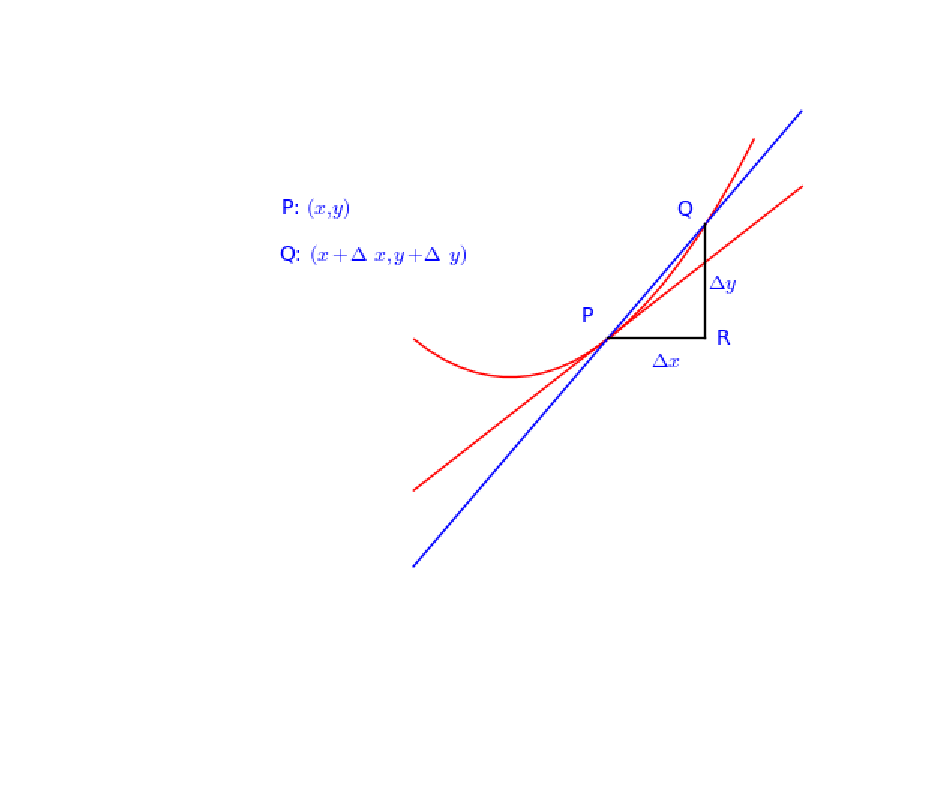
\includegraphics[height=6cm,width=8cm]{parabola-tangent.eps}%
\lthtmlpictureZ
\lthtmlcheckvsize\clearpage}

{\newpage\clearpage
\lthtmlinlinemathA{tex2html_wrap_indisplay45774}%
$\displaystyle y = f(x)$%
\lthtmlindisplaymathZ
\lthtmlcheckvsize\clearpage}

{\newpage\clearpage
\lthtmlinlinemathA{tex2html_wrap_inline45778}%
$ y + \Delta y 	= f(x + \Delta x) 	= NQ$%
\lthtmlinlinemathZ
\lthtmlcheckvsize\clearpage}

{\newpage\clearpage
\lthtmldisplayA{displaymath45780}%
\begin{displaymath}
\begin{array}{ll}
y + \Delta y &	= f(x + \Delta x) 	= NQ\\
  	y &	= f(x) 	= MP = NR\\
  	\Delta y &=	f(x + \Delta x) − f(x) 	= RQ.
\end{array}
\end{displaymath}%
\lthtmldisplayZ
\lthtmlcheckvsize\clearpage}

{\newpage\clearpage
\lthtmldisplayA{displaymath45782}%
\begin{displaymath}
\begin{array}{ll}
\frac{\Delta y}{\Delta x} &	= \frac{f(x + \Delta x) - f(x)}{\Delta x} = \frac{RQ}{MN} = \frac{RQ}{PR}\\
&  	= \tan RPQ = \tan \phi \\
&  	= {\rm slope\  of\  secant\  line\  } PQ.
\end{array}
\end{displaymath}%
\lthtmldisplayZ
\lthtmlcheckvsize\clearpage}

{\newpage\clearpage
\lthtmldisplayA{displaymath45784}%
\begin{displaymath}
\begin{array}{ll}
	\lim_{\Delta x \to 0} \frac{\Delta y}{\Delta x} 
&= \lim_{\Delta x \to 0} \frac{f(x + \Delta x) - f(x)}{\Delta x}\\
& 	= \frac{dy}{dx} = {\rm value\  of\  the\  derivative\  at\  } P.
\end{array}
\end{displaymath}%
\lthtmldisplayZ
\lthtmlcheckvsize\clearpage}

{\newpage\clearpage
\lthtmlinlinemathA{tex2html_wrap_inline45786}%
$ \Delta x \to 0$%
\lthtmlinlinemathZ
\lthtmlcheckvsize\clearpage}

{\newpage\clearpage
\lthtmlinlinemathA{tex2html_wrap_inline45788}%
$ Q$%
\lthtmlinlinemathZ
\lthtmlcheckvsize\clearpage}

{\newpage\clearpage
\lthtmldisplayA{displaymath45794}%
\begin{displaymath}
\begin{array}{ll}
  	\lim_{\Delta x \to 0} \frac{\Delta y}{\Delta x} &= \lim_{\Delta x \to 0} \tan \phi = \tan \tau\\
&  	= {\rm slope\  of\  the\  tangent\  at\  } P.
\end{array}
\end{displaymath}%
\lthtmldisplayZ
\lthtmlcheckvsize\clearpage}

{\newpage\clearpage
\lthtmlinlinemathA{tex2html_wrap_inline45798}%
$ PT$%
\lthtmlinlinemathZ
\lthtmlcheckvsize\clearpage}

{\newpage\clearpage
\lthtmlinlinemathA{tex2html_wrap_inline45814}%
$ x = \frac{1}{2}$%
\lthtmlinlinemathZ
\lthtmlcheckvsize\clearpage}

{\newpage\clearpage
\lthtmlinlinemathA{tex2html_wrap_indisplay45816}%
$\displaystyle y' = \frac{dy}{dx} = 2x = {\rm slope\  of\  tangent\  line\  at\  any\  point\  on\  curve}.
$%
\lthtmlindisplaymathZ
\lthtmlcheckvsize\clearpage}

{\newpage\clearpage
\lthtmlpictureA{tex2html_wrap45818}%
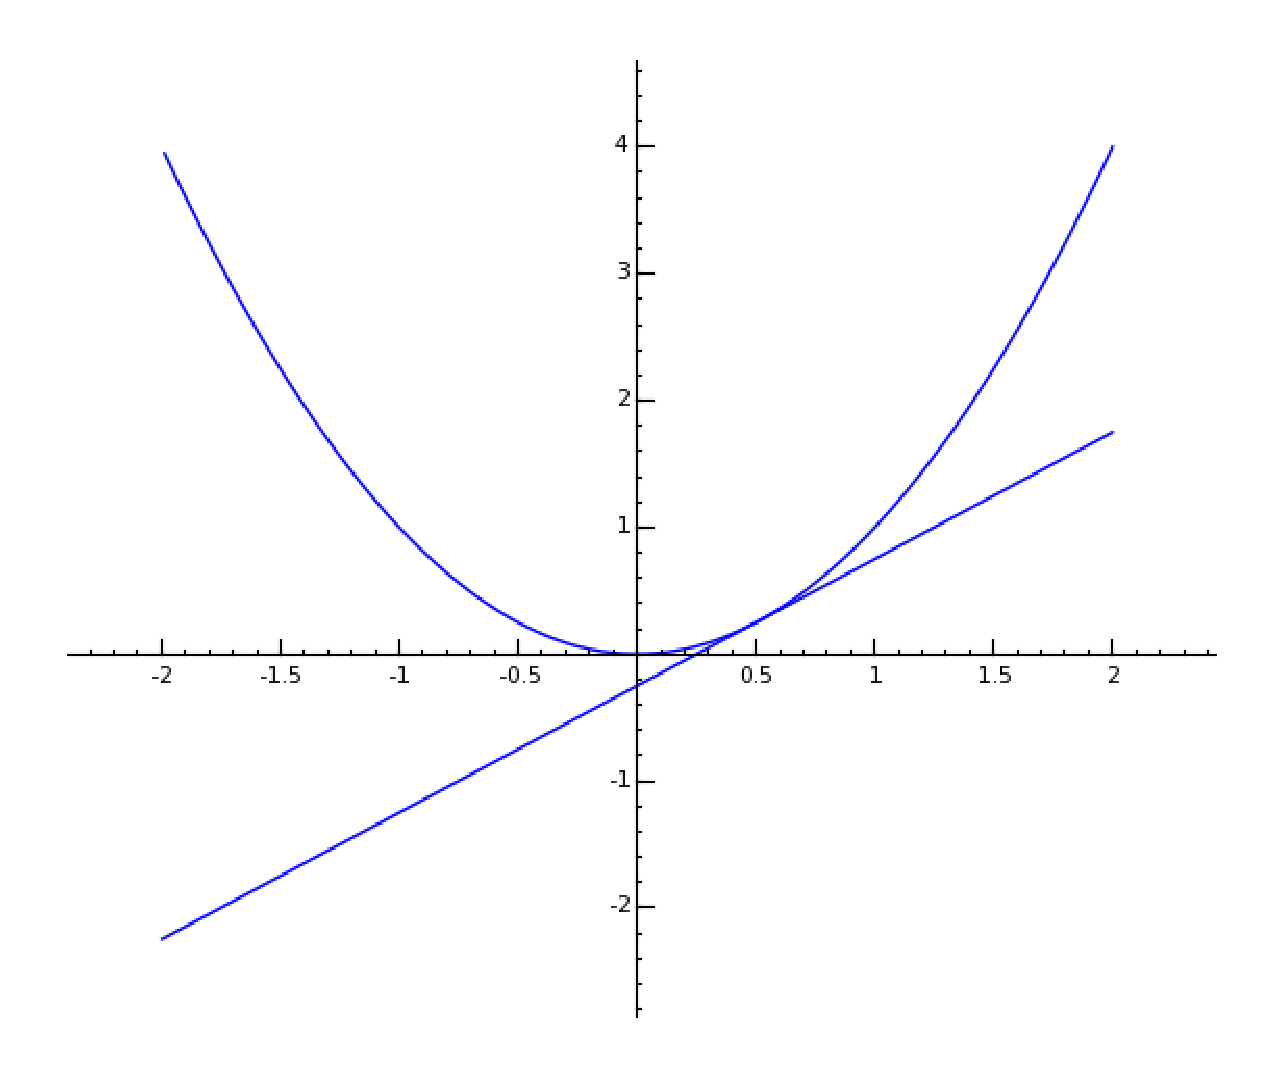
\includegraphics[height=8cm,width=4cm]{deriv-x2.eps}%
\lthtmlpictureZ
\lthtmlcheckvsize\clearpage}

{\newpage\clearpage
\lthtmlinlinemathA{tex2html_wrap_inline45829}%
$ y'=2x$%
\lthtmlinlinemathZ
\lthtmlcheckvsize\clearpage}

{\newpage\clearpage
\lthtmlinlinemathA{tex2html_wrap_indisplay45831}%
$\displaystyle \frac{dy}{dx} = 0.
$%
\lthtmlindisplaymathZ
\lthtmlcheckvsize\clearpage}

{\newpage\clearpage
\lthtmlinlinemathA{tex2html_wrap_indisplay45841}%
$\displaystyle \frac{dy}{dx} = 1;
$%
\lthtmlindisplaymathZ
\lthtmlcheckvsize\clearpage}

{\newpage\clearpage
\lthtmlinlinemathA{tex2html_wrap_inline45845}%
$ 45^o$%
\lthtmlinlinemathZ
\lthtmlcheckvsize\clearpage}

\stepcounter{section}
{\newpage\clearpage
\lthtmlinlinemathA{tex2html_wrap_inline45859}%
$ y = x^2 - 4$%
\lthtmlinlinemathZ
\lthtmlcheckvsize\clearpage}

{\newpage\clearpage
\lthtmlinlinemathA{tex2html_wrap_inline45865}%
$ y = 6 − 3x^2$%
\lthtmlinlinemathZ
\lthtmlcheckvsize\clearpage}

{\newpage\clearpage
\lthtmlinlinemathA{tex2html_wrap_inline45869}%
$ -6$%
\lthtmlinlinemathZ
\lthtmlcheckvsize\clearpage}

{\newpage\clearpage
\lthtmlinlinemathA{tex2html_wrap_inline45873}%
$ x = -1$%
\lthtmlinlinemathZ
\lthtmlcheckvsize\clearpage}

{\newpage\clearpage
\lthtmlinlinemathA{tex2html_wrap_inline45875}%
$ -3$%
\lthtmlinlinemathZ
\lthtmlcheckvsize\clearpage}

{\newpage\clearpage
\lthtmlinlinemathA{tex2html_wrap_inline45877}%
$ y = \frac{2}{x}$%
\lthtmlinlinemathZ
\lthtmlcheckvsize\clearpage}

{\newpage\clearpage
\lthtmlinlinemathA{tex2html_wrap_inline45881}%
$ -\frac{1}{2}$%
\lthtmlinlinemathZ
\lthtmlcheckvsize\clearpage}

{\newpage\clearpage
\lthtmlinlinemathA{tex2html_wrap_inline45883}%
$ y = x - x^2$%
\lthtmlinlinemathZ
\lthtmlcheckvsize\clearpage}

{\newpage\clearpage
\lthtmlinlinemathA{tex2html_wrap_inline45889}%
$ y = \frac{1}{x - 1}$%
\lthtmlinlinemathZ
\lthtmlcheckvsize\clearpage}

{\newpage\clearpage
\lthtmlinlinemathA{tex2html_wrap_inline45893}%
$ -\frac{1}{4}$%
\lthtmlinlinemathZ
\lthtmlcheckvsize\clearpage}

{\newpage\clearpage
\lthtmlinlinemathA{tex2html_wrap_inline45895}%
$ y = \frac{1}{2} x^2$%
\lthtmlinlinemathZ
\lthtmlcheckvsize\clearpage}

{\newpage\clearpage
\lthtmlinlinemathA{tex2html_wrap_inline45897}%
$ x = 4$%
\lthtmlinlinemathZ
\lthtmlcheckvsize\clearpage}

{\newpage\clearpage
\lthtmlinlinemathA{tex2html_wrap_inline45901}%
$ y = x^2 - 2x + 3$%
\lthtmlinlinemathZ
\lthtmlcheckvsize\clearpage}

{\newpage\clearpage
\lthtmlinlinemathA{tex2html_wrap_inline45906}%
$ y = 9 − x^2$%
\lthtmlinlinemathZ
\lthtmlcheckvsize\clearpage}

{\newpage\clearpage
\lthtmlinlinemathA{tex2html_wrap_inline45908}%
$ x = -3$%
\lthtmlinlinemathZ
\lthtmlcheckvsize\clearpage}

{\newpage\clearpage
\lthtmlinlinemathA{tex2html_wrap_inline45910}%
$ 6$%
\lthtmlinlinemathZ
\lthtmlcheckvsize\clearpage}

{\newpage\clearpage
\lthtmlinlinemathA{tex2html_wrap_inline45912}%
$ y = 2x^3 - 6x + 5$%
\lthtmlinlinemathZ
\lthtmlcheckvsize\clearpage}

{\newpage\clearpage
\lthtmlinlinemathA{tex2html_wrap_inline45921}%
$ y = 3x^2 - 1$%
\lthtmlinlinemathZ
\lthtmlcheckvsize\clearpage}

{\newpage\clearpage
\lthtmlinlinemathA{tex2html_wrap_inline45923}%
$ y = 2x^2 + 3$%
\lthtmlinlinemathZ
\lthtmlcheckvsize\clearpage}

{\newpage\clearpage
\lthtmlinlinemathA{tex2html_wrap_inline45925}%
$ \pm 12$%
\lthtmlinlinemathZ
\lthtmlcheckvsize\clearpage}

{\newpage\clearpage
\lthtmlinlinemathA{tex2html_wrap_inline45927}%
$ \pm 8$%
\lthtmlinlinemathZ
\lthtmlcheckvsize\clearpage}

{\newpage\clearpage
\lthtmlinlinemathA{tex2html_wrap_inline45929}%
$ \arctan \frac{4}{97}$%
\lthtmlinlinemathZ
\lthtmlcheckvsize\clearpage}

{\newpage\clearpage
\lthtmlinlinemathA{tex2html_wrap_inline45957}%
$ 30^o$%
\lthtmlinlinemathZ
\lthtmlcheckvsize\clearpage}

{\newpage\clearpage
\lthtmlinlinemathA{tex2html_wrap_inline45959}%
$ \frac{1}{12}$%
\lthtmlinlinemathZ
\lthtmlcheckvsize\clearpage}

{\newpage\clearpage
\lthtmlinlinemathA{tex2html_wrap_inline45980}%
$ \frac{1}{\sqrt{3}}$%
\lthtmlinlinemathZ
\lthtmlcheckvsize\clearpage}

{\newpage\clearpage
\lthtmlinlinemathA{tex2html_wrap_inline45992}%
$ 27^o$%
\lthtmlinlinemathZ
\lthtmlcheckvsize\clearpage}

{\newpage\clearpage
\lthtmlinlinemathA{tex2html_wrap_inline45994}%
$ 43'$%
\lthtmlinlinemathZ
\lthtmlcheckvsize\clearpage}

\stepcounter{chapter}
\stepcounter{section}
{\newpage\clearpage
\lthtmlinlinemathA{tex2html_wrap_inline46011}%
$ u$%
\lthtmlinlinemathZ
\lthtmlcheckvsize\clearpage}

{\newpage\clearpage
\lthtmlinlinemathA{tex2html_wrap_inline46015}%
$ w$%
\lthtmlinlinemathZ
\lthtmlcheckvsize\clearpage}

{\newpage\clearpage
\lthtmlinlinemathA{tex2html_wrap_inline46019}%
$ \frac{dc}{dx} 	= 0$%
\lthtmlinlinemathZ
\lthtmlcheckvsize\clearpage}

{\newpage\clearpage
\lthtmlinlinemathA{tex2html_wrap_inline46021}%
$ \frac{dx}{dx} 	= 1$%
\lthtmlinlinemathZ
\lthtmlcheckvsize\clearpage}

{\newpage\clearpage
\lthtmlinlinemathA{tex2html_wrap_inline46023}%
$ \frac{d}{dx}(u + v - w) 	= \frac{du}{dx}\  +\  \frac{dv}{dx}\  -\  \frac{dw}{dx}$%
\lthtmlinlinemathZ
\lthtmlcheckvsize\clearpage}

{\newpage\clearpage
\lthtmlinlinemathA{tex2html_wrap_inline46025}%
$ \frac{d}{dx} (cv) 	= c \frac{dv}{dx}$%
\lthtmlinlinemathZ
\lthtmlcheckvsize\clearpage}

{\newpage\clearpage
\lthtmlinlinemathA{tex2html_wrap_inline46027}%
$ \frac{d}{dx} (uv) 	= u\frac{dv}{dx}\  +\  v\frac{du}{dx}$%
\lthtmlinlinemathZ
\lthtmlcheckvsize\clearpage}

{\newpage\clearpage
\lthtmlinlinemathA{tex2html_wrap_inline46049}%
$ {\rm vers}$%
\lthtmlinlinemathZ
\lthtmlcheckvsize\clearpage}

{\newpage\clearpage
\lthtmlinlinemathA{tex2html_wrap_inline46051}%
$ {\rm vers}\  v=1-\cos\  v$%
\lthtmlinlinemathZ
\lthtmlcheckvsize\clearpage}

{\newpage\clearpage
\lthtmlinlinemathA{tex2html_wrap_inline46053}%
$ \frac{d}{dx} \left ( v^n \right ) = nv^{n-1} \frac{dv}{dx}$%
\lthtmlinlinemathZ
\lthtmlcheckvsize\clearpage}

{\newpage\clearpage
\lthtmlinlinemathA{tex2html_wrap_inline46055}%
$ \frac{d}{dx} \left ( x^n \right ) = nx^{n - 1}$%
\lthtmlinlinemathZ
\lthtmlcheckvsize\clearpage}

{\newpage\clearpage
\lthtmlinlinemathA{tex2html_wrap_inline46057}%
$ \frac{d}{dx} \left ( \frac{u}{v} \right ) = \frac{v\frac{du}{dx}\  -\  u\frac{dv}{dx}}{v^2}$%
\lthtmlinlinemathZ
\lthtmlcheckvsize\clearpage}

{\newpage\clearpage
\lthtmlinlinemathA{tex2html_wrap_inline46059}%
$ \frac{d}{dx} \left ( \frac{u}{c} \right ) = \frac{\frac{du}{dx}}{c}$%
\lthtmlinlinemathZ
\lthtmlcheckvsize\clearpage}

{\newpage\clearpage
\lthtmlinlinemathA{tex2html_wrap_inline46061}%
$ \frac{d}{dx} \left ( \log_a v \right ) = \log_a\  e\  \cdot\  \frac{\frac{dv}{dx}}{v}$%
\lthtmlinlinemathZ
\lthtmlcheckvsize\clearpage}

{\newpage\clearpage
\lthtmlinlinemathA{tex2html_wrap_inline46063}%
$ \frac{d}{dx} \left ( a^v \right ) = a^v\  \log\  a\  \frac{dv}{dx}$%
\lthtmlinlinemathZ
\lthtmlcheckvsize\clearpage}

{\newpage\clearpage
\lthtmlinlinemathA{tex2html_wrap_inline46065}%
$ \frac{d}{dx} \left ( e^v \right ) = e^v \frac{dv}{dx}$%
\lthtmlinlinemathZ
\lthtmlcheckvsize\clearpage}

{\newpage\clearpage
\lthtmlinlinemathA{tex2html_wrap_inline46067}%
$ \frac{d}{dx} \left ( u^v \right ) = vu^{v-1} \frac{du}{dx}\  +\  \log\  u\  \cdot\  u^v \frac{dv}{dx}$%
\lthtmlinlinemathZ
\lthtmlcheckvsize\clearpage}

{\newpage\clearpage
\lthtmlinlinemathA{tex2html_wrap_inline46069}%
$ \frac{d}{dx} (\sin\  v) = \cos\  v \frac{dv}{dx}$%
\lthtmlinlinemathZ
\lthtmlcheckvsize\clearpage}

{\newpage\clearpage
\lthtmlinlinemathA{tex2html_wrap_inline46071}%
$ \frac{d}{dx}(\cos\  v) = -\sin\  v \frac{dv}{dx}$%
\lthtmlinlinemathZ
\lthtmlcheckvsize\clearpage}

{\newpage\clearpage
\lthtmlinlinemathA{tex2html_wrap_inline46073}%
$ \frac{d}{dx}(\tan\  v) =	\sec^2 v \frac{dv}{dx}$%
\lthtmlinlinemathZ
\lthtmlcheckvsize\clearpage}

{\newpage\clearpage
\lthtmlinlinemathA{tex2html_wrap_inline46075}%
$ \frac{d}{dx}(\cot\  x) 	= -\csc^2 v \frac{dv}{dx}$%
\lthtmlinlinemathZ
\lthtmlcheckvsize\clearpage}

{\newpage\clearpage
\lthtmlinlinemathA{tex2html_wrap_inline46077}%
$ \frac{d}{dx}(\sec\  v) 	= \sec\  v\  \tan\  v \frac{dv}{dx}$%
\lthtmlinlinemathZ
\lthtmlcheckvsize\clearpage}

{\newpage\clearpage
\lthtmlinlinemathA{tex2html_wrap_inline46079}%
$ \frac{d}{dx} (\csc\  v) 	= -\csc\  v\  \cot\  v \frac{dv}{dx}$%
\lthtmlinlinemathZ
\lthtmlcheckvsize\clearpage}

{\newpage\clearpage
\lthtmlinlinemathA{tex2html_wrap_inline46081}%
$ \frac{d}{dx} ({\rm vers}\  v) = \sin\  v \frac{dv}{dx}$%
\lthtmlinlinemathZ
\lthtmlcheckvsize\clearpage}

{\newpage\clearpage
\lthtmlinlinemathA{tex2html_wrap_inline46083}%
$ \frac{d}{dx} (\arcsin\  v) = \frac{\frac{dv}{dx}}{\sqrt{1 - v^2}}$%
\lthtmlinlinemathZ
\lthtmlcheckvsize\clearpage}

{\newpage\clearpage
\lthtmlinlinemathA{tex2html_wrap_inline46085}%
$ \frac{d}{dx} (\arccos\  v) = -\frac{\frac{dv}{dx}}{\sqrt{1 - v^2}}$%
\lthtmlinlinemathZ
\lthtmlcheckvsize\clearpage}

{\newpage\clearpage
\lthtmlinlinemathA{tex2html_wrap_inline46087}%
$ \frac{d}{dx} (\arctan\  v) = \frac{\frac{dv}{dx}}{1 + v^2}$%
\lthtmlinlinemathZ
\lthtmlcheckvsize\clearpage}

{\newpage\clearpage
\lthtmlinlinemathA{tex2html_wrap_inline46089}%
$ \frac{d}{dx} ({\rm arccot}\  v) = -\frac{\frac{dv}{dx}}{1 + v^2}$%
\lthtmlinlinemathZ
\lthtmlcheckvsize\clearpage}

{\newpage\clearpage
\lthtmlinlinemathA{tex2html_wrap_inline46165}%
$ \arcsin$%
\lthtmlinlinemathZ
\lthtmlcheckvsize\clearpage}

{\newpage\clearpage
\lthtmlinlinemathA{tex2html_wrap_inline46167}%
$ \arccos$%
\lthtmlinlinemathZ
\lthtmlcheckvsize\clearpage}

{\newpage\clearpage
\lthtmlinlinemathA{tex2html_wrap_inline46169}%
$ {\rm asin}$%
\lthtmlinlinemathZ
\lthtmlcheckvsize\clearpage}

{\newpage\clearpage
\lthtmlinlinemathA{tex2html_wrap_inline46171}%
$ {\rm acos}$%
\lthtmlinlinemathZ
\lthtmlcheckvsize\clearpage}

{\newpage\clearpage
\lthtmlinlinemathA{tex2html_wrap_inline46173}%
$ \frac{d}{dx} ({\rm arcsec}\  v) = \frac{\frac{dv}{dx}}{v \sqrt{v^2 - 1}}$%
\lthtmlinlinemathZ
\lthtmlcheckvsize\clearpage}

{\newpage\clearpage
\lthtmlinlinemathA{tex2html_wrap_inline46175}%
$ \frac{d}{dx} ({\rm arccsc}\  v) = -\frac{\frac{dv}{dx}}{v\sqrt{v^2 - 1}}$%
\lthtmlinlinemathZ
\lthtmlcheckvsize\clearpage}

{\newpage\clearpage
\lthtmlinlinemathA{tex2html_wrap_inline46177}%
$ \frac{d}{dx} (\operatorname{arcvers}\  v) = \frac{\frac{dv}{dx}}{\sqrt{2v - v^2}}$%
\lthtmlinlinemathZ
\lthtmlcheckvsize\clearpage}

{\newpage\clearpage
\lthtmlinlinemathA{tex2html_wrap_inline46179}%
$ \frac{dy}{dx} 	= \frac{dy}{dv} \cdot \frac{dv}{dx}$%
\lthtmlinlinemathZ
\lthtmlcheckvsize\clearpage}

{\newpage\clearpage
\lthtmlinlinemathA{tex2html_wrap_inline46185}%
$ \frac{dy}{dx} 	= \frac{1}{\frac{dx}{dy}}$%
\lthtmlinlinemathZ
\lthtmlcheckvsize\clearpage}

{\newpage\clearpage
\lthtmlinlinemathA{tex2html_wrap_inline46209}%
$ \frac{d \arccos\, t}{dt}=-\frac{1}{\sqrt{1-t^2}}$%
\lthtmlinlinemathZ
\lthtmlcheckvsize\clearpage}

{\newpage\clearpage
\lthtmlinlinemathA{tex2html_wrap_inline46211}%
$ \frac{d {\rm arccsc}\, v}{dv}=-\frac{1}{v\sqrt{v^2-1}}$%
\lthtmlinlinemathZ
\lthtmlcheckvsize\clearpage}

\stepcounter{section}
{\newpage\clearpage
\lthtmlinlinemathA{tex2html_wrap_indisplay46216}%
$\displaystyle y 	= c.
$%
\lthtmlindisplaymathZ
\lthtmlcheckvsize\clearpage}

{\newpage\clearpage
\lthtmlinlinemathA{tex2html_wrap_inline46222}%
$ \Delta y = 0$%
\lthtmlinlinemathZ
\lthtmlcheckvsize\clearpage}

{\newpage\clearpage
\lthtmlinlinemathA{tex2html_wrap_indisplay46224}%
$\displaystyle \frac{\Delta y}{\Delta x} 	= 0.
$%
\lthtmlindisplaymathZ
\lthtmlcheckvsize\clearpage}

{\newpage\clearpage
\lthtmlinlinemathA{tex2html_wrap_indisplay46226}%
$\displaystyle \lim_{\Delta x \to 0} \left ( \frac{\Delta y}{\Delta x} \right )
= \frac{dy}{dx} = 0.
$%
\lthtmlindisplaymathZ
\lthtmlcheckvsize\clearpage}

\stepcounter{section}
{\newpage\clearpage
\lthtmlinlinemathA{tex2html_wrap_inline46231}%
$ y 	= x$%
\lthtmlinlinemathZ
\lthtmlcheckvsize\clearpage}

{\newpage\clearpage
\lthtmlinlinemathA{tex2html_wrap_inline46233}%
$ y + \Delta y = x + \Delta x$%
\lthtmlinlinemathZ
\lthtmlcheckvsize\clearpage}

{\newpage\clearpage
\lthtmlinlinemathA{tex2html_wrap_inline46235}%
$ \Delta y = \Delta x$%
\lthtmlinlinemathZ
\lthtmlcheckvsize\clearpage}

{\newpage\clearpage
\lthtmlinlinemathA{tex2html_wrap_inline46237}%
$ \frac{\Delta y}{\Delta x} = 1$%
\lthtmlinlinemathZ
\lthtmlcheckvsize\clearpage}

{\newpage\clearpage
\lthtmlinlinemathA{tex2html_wrap_inline46239}%
$ \frac{dy}{dx} 	= 1$%
\lthtmlinlinemathZ
\lthtmlcheckvsize\clearpage}

\stepcounter{section}
{\newpage\clearpage
\lthtmlinlinemathA{tex2html_wrap_inline46244}%
$ y 	= u + v - w$%
\lthtmlinlinemathZ
\lthtmlcheckvsize\clearpage}

{\newpage\clearpage
\lthtmlinlinemathA{tex2html_wrap_inline46246}%
$ y + \Delta y = u + \Delta u + v + \Delta v - w - \Delta w$%
\lthtmlinlinemathZ
\lthtmlcheckvsize\clearpage}

{\newpage\clearpage
\lthtmlinlinemathA{tex2html_wrap_inline46248}%
$ \Delta y 	= \Delta u + \Delta v - \Delta w$%
\lthtmlinlinemathZ
\lthtmlcheckvsize\clearpage}

{\newpage\clearpage
\lthtmlinlinemathA{tex2html_wrap_inline46250}%
$ \frac{\Delta y}{\Delta x} 	
= \frac{\Delta u}{\Delta x} + \frac{\Delta v}{\Delta x} 
- \frac{\Delta w}{\Delta x}$%
\lthtmlinlinemathZ
\lthtmlcheckvsize\clearpage}

{\newpage\clearpage
\lthtmlinlinemathA{tex2html_wrap_inline46252}%
$ \frac{dy}{dx} = \frac{du}{dx} + \frac{dv}{dx} - \frac{dw}{dx}$%
\lthtmlinlinemathZ
\lthtmlcheckvsize\clearpage}

\stepcounter{section}
{\newpage\clearpage
\lthtmlinlinemathA{tex2html_wrap_inline46257}%
$ y 	= cv$%
\lthtmlinlinemathZ
\lthtmlcheckvsize\clearpage}

{\newpage\clearpage
\lthtmlinlinemathA{tex2html_wrap_inline46259}%
$ y + \Delta y = c(v + \Delta v) = cv + c\Delta v$%
\lthtmlinlinemathZ
\lthtmlcheckvsize\clearpage}

{\newpage\clearpage
\lthtmlinlinemathA{tex2html_wrap_inline46261}%
$ \Delta y = c \cdot \Delta v$%
\lthtmlinlinemathZ
\lthtmlcheckvsize\clearpage}

{\newpage\clearpage
\lthtmlinlinemathA{tex2html_wrap_inline46263}%
$ \frac{\Delta y}{\Delta x} 	= c\frac{\Delta v}{\Delta x}$%
\lthtmlinlinemathZ
\lthtmlcheckvsize\clearpage}

{\newpage\clearpage
\lthtmlinlinemathA{tex2html_wrap_inline46265}%
$ \frac{dy}{dx} = c\frac{dv}{dx}$%
\lthtmlinlinemathZ
\lthtmlcheckvsize\clearpage}

\stepcounter{section}
{\newpage\clearpage
\lthtmlinlinemathA{tex2html_wrap_inline46270}%
$ y 	= uv$%
\lthtmlinlinemathZ
\lthtmlcheckvsize\clearpage}

{\newpage\clearpage
\lthtmlinlinemathA{tex2html_wrap_inline46272}%
$ y + \Delta y 	= (u + \Delta u)(v + \Delta v)$%
\lthtmlinlinemathZ
\lthtmlcheckvsize\clearpage}

{\newpage\clearpage
\lthtmlinlinemathA{tex2html_wrap_indisplay46274}%
$\displaystyle y + \Delta y 	= uv + u \cdot \Delta v + v \cdot \Delta u + \Delta u \cdot \Delta v.
$%
\lthtmlindisplaymathZ
\lthtmlcheckvsize\clearpage}

{\newpage\clearpage
\lthtmlinlinemathA{tex2html_wrap_inline46276}%
$ \Delta y 
= u \cdot \Delta v + v \cdot \Delta u + \Delta u \cdot \Delta v$%
\lthtmlinlinemathZ
\lthtmlcheckvsize\clearpage}

{\newpage\clearpage
\lthtmlinlinemathA{tex2html_wrap_inline46278}%
$ \frac{\Delta y}{\Delta x} 
= u \frac{\Delta v}{\Delta x} + v \frac{\Delta u}{\Delta x} 
+ \Delta u \frac{\Delta v}{\Delta x}$%
\lthtmlinlinemathZ
\lthtmlcheckvsize\clearpage}

{\newpage\clearpage
\lthtmlinlinemathA{tex2html_wrap_inline46280}%
$ \frac{dy}{dx} 	= u \frac{dv}{dx} + v \frac{du}{dx}$%
\lthtmlinlinemathZ
\lthtmlcheckvsize\clearpage}

{\newpage\clearpage
\lthtmlinlinemathA{tex2html_wrap_inline46284}%
$ \Delta u \to 0$%
\lthtmlinlinemathZ
\lthtmlcheckvsize\clearpage}

{\newpage\clearpage
\lthtmlinlinemathA{tex2html_wrap_inline46286}%
$ \left ( \Delta u \frac{\Delta v}{\Delta x} \right ) \to 0$%
\lthtmlinlinemathZ
\lthtmlcheckvsize\clearpage}

{\newpage\clearpage
\lthtmlinlinemathA{tex2html_wrap_inline46290}%
$ \frac{d}{dt}(e^{2t}\cos(t)$%
\lthtmlinlinemathZ
\lthtmlcheckvsize\clearpage}

\stepcounter{section}
{\newpage\clearpage
\lthtmlinlinemathA{tex2html_wrap_inline46293}%
$ uv$%
\lthtmlinlinemathZ
\lthtmlcheckvsize\clearpage}

{\newpage\clearpage
\lthtmlinlinemathA{tex2html_wrap_indisplay46295}%
$\displaystyle \frac{\frac{d}{dx}(uv)}{uv} 	= \frac{\frac{du}{dx}}{u} + \frac{\frac{dv}{dx}}{v}.
$%
\lthtmlindisplaymathZ
\lthtmlcheckvsize\clearpage}

{\newpage\clearpage
\lthtmlinlinemathA{tex2html_wrap_inline46299}%
$ y 	= v_1 v_2 \cdots v_n$%
\lthtmlinlinemathZ
\lthtmlcheckvsize\clearpage}

{\newpage\clearpage
\lthtmldisplayA{displaymath46301}%
\begin{displaymath}
\begin{array}{ll}
\frac{\frac{d}{dx}(v_1 v_2 \cdots v_n)}{v_1 v_2 \cdots v_n} 	
&= \frac{\frac{dv_1}{dx}}{v_1} + \frac{\frac{d}{dx} (v_2 v_3 \cdots v_n)}{v_2 v_3 \cdots v_n}\\
&  	= \frac{\frac{dv_1}{dx}}{v_1} + \frac{\frac{dv_2}{dx}}{v_2} + \frac{\frac{d}{dx} (v_3 v_4 \cdots v_n)}{v_3 v_4 \cdots v_n}\\
& 	= \frac{\frac{dv_1}{dx}}{v_1} + \frac{\frac{dv_2}{dx}}{v_2} + \frac{\frac{dv_3}{dx}}{v_3} + \cdots + \frac{\frac{dv_n}{dx}}{v_n}
\frac{d}{dx} (v_1 v_2 \cdots v_n) \\
&	= (v_2 v_3 \cdots v_n)\frac{dv_1}{dx} + (v_1 v_3 \cdots v_n)\frac{dv_2}{dx} + \cdots
  	+ (v_1 v_2 \cdots v_{n - 1})\frac{dv_n}{dx}.
\end{array}
\end{displaymath}%
\lthtmldisplayZ
\lthtmlcheckvsize\clearpage}

\stepcounter{section}
{\newpage\clearpage
\lthtmlinlinemathA{tex2html_wrap_indisplay46308}%
$\displaystyle \frac{\frac{d}{dx}(v^n)}{v^n} 	= n\frac{\frac{dv}{dx}}{v}.
$%
\lthtmlindisplaymathZ
\lthtmlcheckvsize\clearpage}

{\newpage\clearpage
\lthtmlinlinemathA{tex2html_wrap_inline46310}%
$ \frac{d}{dx}(v^n) 	= nv^{n-1}\frac{dv}{dx}$%
\lthtmlinlinemathZ
\lthtmlcheckvsize\clearpage}

{\newpage\clearpage
\lthtmlinlinemathA{tex2html_wrap_inline46312}%
$ v = x$%
\lthtmlinlinemathZ
\lthtmlcheckvsize\clearpage}

{\newpage\clearpage
\lthtmlinlinemathA{tex2html_wrap_inline46314}%
$ \frac{d}{dx}(x^n) 	= nx^{n - 1}$%
\lthtmlinlinemathZ
\lthtmlcheckvsize\clearpage}

\stepcounter{section}
{\newpage\clearpage
\lthtmlinlinemathA{tex2html_wrap_inline46321}%
$ y 	= \frac{u}{v} 	v \ne 0$%
\lthtmlinlinemathZ
\lthtmlcheckvsize\clearpage}

{\newpage\clearpage
\lthtmlinlinemathA{tex2html_wrap_inline46323}%
$ y + \Delta y 	= \frac{u + \Delta u}{v + \Delta v}$%
\lthtmlinlinemathZ
\lthtmlcheckvsize\clearpage}

{\newpage\clearpage
\lthtmlinlinemathA{tex2html_wrap_inline46325}%
$ \Delta y 	= \frac{u + \Delta u}{v \Delta v} - \frac{u}{v} = \frac{v \cdot \Delta u - u \cdot \Delta v}{v(v + \Delta v)}$%
\lthtmlinlinemathZ
\lthtmlcheckvsize\clearpage}

{\newpage\clearpage
\lthtmlinlinemathA{tex2html_wrap_inline46327}%
$ \frac{\Delta y}{\Delta x} 	= \frac{v\frac{\Delta u}{\Delta x} - u\frac{\Delta v}{\Delta x}}{v(v + \Delta v)}$%
\lthtmlinlinemathZ
\lthtmlcheckvsize\clearpage}

{\newpage\clearpage
\lthtmlinlinemathA{tex2html_wrap_inline46329}%
$ \frac{dy}{dx} 	= \frac{v\frac{du}{dx} - u\frac{dv}{dx}}{v^2}$%
\lthtmlinlinemathZ
\lthtmlcheckvsize\clearpage}

{\newpage\clearpage
\lthtmlinlinemathA{tex2html_wrap_inline46331}%
$ \frac{d}{dx} \left ( \frac{u}{v} \right ) 
\frac{v\frac{du}{dx} - u\frac{dv}{dx}}{v^2}$%
\lthtmlinlinemathZ
\lthtmlcheckvsize\clearpage}

{\newpage\clearpage
\lthtmlinlinemathA{tex2html_wrap_inline46333}%
$ v = c$%
\lthtmlinlinemathZ
\lthtmlcheckvsize\clearpage}

{\newpage\clearpage
\lthtmlinlinemathA{tex2html_wrap_inline46337}%
$ \frac{dv}{dx} = \frac{dc}{dx} = 0$%
\lthtmlinlinemathZ
\lthtmlcheckvsize\clearpage}

{\newpage\clearpage
\lthtmlinlinemathA{tex2html_wrap_indisplay46339}%
$\displaystyle \frac{d}{dx} \left ( \frac{u}{c} \right ) 	
= \frac{1}{c} \frac{du}{dx} = \frac{\frac{du}{dx}}{c}.
$%
\lthtmlindisplaymathZ
\lthtmlcheckvsize\clearpage}

\stepcounter{section}
{\newpage\clearpage
\lthtmlinlinemathA{tex2html_wrap_inline46348}%
$ \frac{dy}{dx} = \frac{d}{dx}(x^3) = 3x^2$%
\lthtmlinlinemathZ
\lthtmlcheckvsize\clearpage}

{\newpage\clearpage
\lthtmlinlinemathA{tex2html_wrap_inline46350}%
$ y = ax^4 - bx^2$%
\lthtmlinlinemathZ
\lthtmlcheckvsize\clearpage}

{\newpage\clearpage
\lthtmldisplayA{displaymath46352}%
\begin{displaymath}
\begin{array}{ll}
\frac{dy}{dx} &	= \frac{d}{dx} (ax^4 - bx^2) \\
& = \frac{d}{dx} (ax^4) - \frac{d}{dx}( bx^2) \  \ \  {\rm by\  III}\\
& = a\frac{d}{dx} (x^4) - b\frac{d}{dx} (x^2)  \  \ \  {\rm by\  IV}\\
 & = 4ax^3 - 2bx  \  \ \  {\rm by\  VIa}. 
\end{array}
\end{displaymath}%
\lthtmldisplayZ
\lthtmlcheckvsize\clearpage}

{\newpage\clearpage
\lthtmlinlinemathA{tex2html_wrap_inline46354}%
$ y = x^{\frac{4}{3}} + 5$%
\lthtmlinlinemathZ
\lthtmlcheckvsize\clearpage}

{\newpage\clearpage
\lthtmldisplayA{displaymath46356}%
\begin{displaymath}
\begin{array}{ll}
\frac{dy}{dx} &	= \frac{d}{dx}(x^{\frac{4}{3}}) + \frac{d}{dx}(5) \  \ \  {\rm by\  III}\\
  &	= \frac{4}{3} x^{\frac{1}{3}}  \  \ \  {\rm by\   VIa\  and\  I}
\end{array}
\end{displaymath}%
\lthtmldisplayZ
\lthtmlcheckvsize\clearpage}

{\newpage\clearpage
\lthtmlinlinemathA{tex2html_wrap_inline46358}%
$ y = \frac{3x^3}{\sqrt[5]{x^2}} - \frac{7x}{\sqrt[3]{x^4}} + 8\sqrt[7]{x^3}$%
\lthtmlinlinemathZ
\lthtmlcheckvsize\clearpage}

{\newpage\clearpage
\lthtmldisplayA{displaymath46360}%
\begin{displaymath}
\begin{array}{ll}
\frac{dy}{dx} &	= \frac{d}{dx} \left ( 3 x^{\frac{13}{5}} \right ) 
+ \frac{d}{dx} \left ( 7 x^{-\frac{1}{3}} \right ) 
+ \frac{d}{dx} \left ( 8 x^{\frac{3}{7}} \right )   \  \ \  {\rm by\  III}\\
&  	= \frac{39}{5} x^{\frac{8}{5}} + \frac{7}{3} x^{-\frac{4}{3}} + \frac{24}{7} x^{-\frac{4}{7}}
  \  \ \  {\rm by\   IV\  and\  VIa}.
\end{array}
\end{displaymath}%
\lthtmldisplayZ
\lthtmlcheckvsize\clearpage}

{\newpage\clearpage
\lthtmlinlinemathA{tex2html_wrap_inline46362}%
$ y = (x^2 - 3)^5$%
\lthtmlinlinemathZ
\lthtmlcheckvsize\clearpage}

{\newpage\clearpage
\lthtmldisplayA{displaymath46364}%
\begin{displaymath}
\begin{array}{ll}
\frac{dy}{dx} &=5 (x^2 - 3)^4 \frac{d}{dx} (x^2 - 3)   \  \ \  {\rm by\  VI,
v = x^2 - 3 \  {\rm and\  } n = 5}\\
  	5(x^2 - 3)^4 \cdot 2x & = 10x(x^2 - 3)^4. 
\end{array}
\end{displaymath}%
\lthtmldisplayZ
\lthtmlcheckvsize\clearpage}

{\newpage\clearpage
\lthtmlinlinemathA{tex2html_wrap_inline46366}%
$ y = \sqrt{a^2 - x^2}$%
\lthtmlinlinemathZ
\lthtmlcheckvsize\clearpage}

{\newpage\clearpage
\lthtmldisplayA{displaymath46368}%
\begin{displaymath}
\begin{array}{ll}
\frac{dy}{dx} &=	\frac{d}{dx}(a^2 - x^2)^{\frac{1}{2}}\\
& = \frac{1}{2}(a^2 - x^2)^{-\frac{1}{2}}\frac{d}{dx} (a^2 - x^2),  
\  \ \  {\rm by\  VI}\  (v = a^2 - x^2,\  {\rm and\  }n = 5)\\
& = \frac{1}{2} (a^2 - x^2)^{-\frac{1}{2}} (-2x) = -\frac{x}{\sqrt{a^2 - x^2}}. 
\end{array}
\end{displaymath}%
\lthtmldisplayZ
\lthtmlcheckvsize\clearpage}

{\newpage\clearpage
\lthtmlinlinemathA{tex2html_wrap_inline46370}%
$ y = (3x^2 + 2)\sqrt{1 + 5x^2}$%
\lthtmlinlinemathZ
\lthtmlcheckvsize\clearpage}

{\newpage\clearpage
\lthtmldisplayA{displaymath46372}%
\begin{displaymath}
\begin{array}{ll}
\frac{dy}{dx} &	= (3x^2 + 2) \frac{d}{dx} (1 + 5x^2)^{\frac{1}{2}} 
+ (1 + 5x^2)^{\frac{1}{2}} \frac{d}{dx} (3x^2 + 2)\\
 & \  \ \  \  \  \ \  ({\rm by\  V\  },
u = 3x^2 + 2,\  {\rm and\  } v = (1 + 5x^2)^{\frac{1}{2}})\\
& = (3x^2 + 2) \frac{1}{2} (1 + 5x^2)^{-\frac{1}{2}} \frac{d}{dx} (1 + 5x^2) 
+ (1 + 5x^2)^{\frac{1}{2}} 6x \  \ \  {\rm by\  VI,\  etc.}\\
 & = (3x^2 + 2)(1 + 5x^2)^{-\frac{1}{2}} 5x + 6x(1 + 5x^2)^{\frac{1}{2}}\\
 & = \frac{5x(3x^2 + 2)}{\sqrt{1 + 5x^2}} + 6x\sqrt{1 + 5x^2} \\
& = \frac{45x^3 + 16x}{\sqrt{1 + 5x^2}}. 
\end{array}
\end{displaymath}%
\lthtmldisplayZ
\lthtmlcheckvsize\clearpage}

{\newpage\clearpage
\lthtmlinlinemathA{tex2html_wrap_inline46374}%
$ y = \frac{a^2 + x^2}{\sqrt{a^2 - x^2}}$%
\lthtmlinlinemathZ
\lthtmlcheckvsize\clearpage}

{\newpage\clearpage
\lthtmldisplayA{displaymath46376}%
\begin{displaymath}
\begin{array}{ll}
\frac{dy}{dx} & 	= \frac{(a^2 - x^2)^{\frac{1}{2}} \frac{d}{dx} (a^2 - x^2) - (a^2 + x^2) \frac{d}{dx} (a^2 - x^2)^{\frac{1}{2}}}{a^2 - x^2}  \  \ \  {\rm by\  VII}\\
  &	= \frac{2x(a^2 - x^2) + x(a^2 + x^2)}{(a^2 - x^2)^{-\frac{3}{2}}}\\
 & ({\rm multiplying\  both\  numerator\  and\  denominator\  by\  }(a^2 - x^2)^{\frac{1}{2}})\\
 & = \frac{\frac3 x^2x - x^3}{(a^2 - x^2)^{\frac{3}{2}}}. 
\end{array}
\end{displaymath}%
\lthtmldisplayZ
\lthtmlcheckvsize\clearpage}

{\newpage\clearpage
\lthtmlinlinemathA{tex2html_wrap_inline46378}%
$ 5x^4 + 3x^2 - 6$%
\lthtmlinlinemathZ
\lthtmlcheckvsize\clearpage}

{\newpage\clearpage
\lthtmlinlinemathA{tex2html_wrap_inline46380}%
$ \frac{dy}{dx} = 20x^3 + 6x$%
\lthtmlinlinemathZ
\lthtmlcheckvsize\clearpage}

{\newpage\clearpage
\lthtmlinlinemathA{tex2html_wrap_inline46382}%
$ y = 3cx^2 - 8dx + 5e$%
\lthtmlinlinemathZ
\lthtmlcheckvsize\clearpage}

{\newpage\clearpage
\lthtmlinlinemathA{tex2html_wrap_inline46384}%
$ \frac{dy}{dx} = 6cx - 8d$%
\lthtmlinlinemathZ
\lthtmlcheckvsize\clearpage}

{\newpage\clearpage
\lthtmlinlinemathA{tex2html_wrap_inline46386}%
$ y = x^{a + b}$%
\lthtmlinlinemathZ
\lthtmlcheckvsize\clearpage}

{\newpage\clearpage
\lthtmlinlinemathA{tex2html_wrap_inline46388}%
$ \frac{dy}{dx} = (a + b)x^{a + b - 1}$%
\lthtmlinlinemathZ
\lthtmlcheckvsize\clearpage}

{\newpage\clearpage
\lthtmlinlinemathA{tex2html_wrap_inline46390}%
$ y = x^n + nx + n$%
\lthtmlinlinemathZ
\lthtmlcheckvsize\clearpage}

{\newpage\clearpage
\lthtmlinlinemathA{tex2html_wrap_inline46392}%
$ \frac{dy}{dx} = nx^{n - 1} + n$%
\lthtmlinlinemathZ
\lthtmlcheckvsize\clearpage}

{\newpage\clearpage
\lthtmlinlinemathA{tex2html_wrap_inline46394}%
$ f(x) = \frac{2}{3} x^3 - \frac{3}{2} x^2 + 5$%
\lthtmlinlinemathZ
\lthtmlcheckvsize\clearpage}

{\newpage\clearpage
\lthtmlinlinemathA{tex2html_wrap_inline46396}%
$ f'(x) = 2x^2 - 3x$%
\lthtmlinlinemathZ
\lthtmlcheckvsize\clearpage}

{\newpage\clearpage
\lthtmlinlinemathA{tex2html_wrap_inline46398}%
$ f(x) = (a + b)x^2 + cx + d$%
\lthtmlinlinemathZ
\lthtmlcheckvsize\clearpage}

{\newpage\clearpage
\lthtmlinlinemathA{tex2html_wrap_inline46400}%
$ f'(x) = 2(a + b)x + c$%
\lthtmlinlinemathZ
\lthtmlcheckvsize\clearpage}

{\newpage\clearpage
\lthtmlinlinemathA{tex2html_wrap_inline46402}%
$ \frac{d}{dx}(a + bx + cx^2) = b + 2cx$%
\lthtmlinlinemathZ
\lthtmlcheckvsize\clearpage}

{\newpage\clearpage
\lthtmlinlinemathA{tex2html_wrap_inline46404}%
$ \frac{d}{dy}(5y^m - 3y + 6) = 5my^{m - 1} - 3$%
\lthtmlinlinemathZ
\lthtmlcheckvsize\clearpage}

{\newpage\clearpage
\lthtmlinlinemathA{tex2html_wrap_inline46406}%
$ \frac{d}{dx}(2 x^{-2} + 3x^{-3}) = -4x^{-3} - 9x^{-4}$%
\lthtmlinlinemathZ
\lthtmlcheckvsize\clearpage}

{\newpage\clearpage
\lthtmlinlinemathA{tex2html_wrap_inline46408}%
$ \frac{d}{ds}(3s^{-4} - s) = -12s^{-5} - 1$%
\lthtmlinlinemathZ
\lthtmlcheckvsize\clearpage}

{\newpage\clearpage
\lthtmlinlinemathA{tex2html_wrap_inline46410}%
$ \frac{d}{dx}(4x^{\frac{1}{2}} + x^2) = 2x^{-\frac{1}{2}} + 2x$%
\lthtmlinlinemathZ
\lthtmlcheckvsize\clearpage}

{\newpage\clearpage
\lthtmlinlinemathA{tex2html_wrap_inline46412}%
$ \frac{d}{dy}(y^{-2} - 4y^{-\frac{1}{2}}) = -2y^{-3} + 2y^{-\frac{3}{2}}$%
\lthtmlinlinemathZ
\lthtmlcheckvsize\clearpage}

{\newpage\clearpage
\lthtmlinlinemathA{tex2html_wrap_inline46414}%
$ \frac{d}{dx}(2x^3 + 5) = 6x^2$%
\lthtmlinlinemathZ
\lthtmlcheckvsize\clearpage}

{\newpage\clearpage
\lthtmlinlinemathA{tex2html_wrap_inline46416}%
$ \frac{d}{dt}(3t^5 - 2t^2) = 15t^4 - 4t$%
\lthtmlinlinemathZ
\lthtmlcheckvsize\clearpage}

{\newpage\clearpage
\lthtmlinlinemathA{tex2html_wrap_inline46418}%
$ \frac{d}{d\theta}(a\theta^4 + b\theta) = 4a\theta^3 + b$%
\lthtmlinlinemathZ
\lthtmlcheckvsize\clearpage}

{\newpage\clearpage
\lthtmlinlinemathA{tex2html_wrap_inline46420}%
$ \frac{d}{d\alpha}(5 - 2\alpha^{\frac{3}{2}}) = -3\alpha^{\frac{1}{2}}$%
\lthtmlinlinemathZ
\lthtmlcheckvsize\clearpage}

{\newpage\clearpage
\lthtmlinlinemathA{tex2html_wrap_inline46422}%
$ \frac{d}{dt}(9t^{\frac{5}{3}} + t^{-1}) = 15t^{\frac{2}{3}} - t^{-2}$%
\lthtmlinlinemathZ
\lthtmlcheckvsize\clearpage}

{\newpage\clearpage
\lthtmlinlinemathA{tex2html_wrap_inline46424}%
$ \frac{d}{dx}(2x^{12} - x^9) = 24x^{11} - 9x^8$%
\lthtmlinlinemathZ
\lthtmlcheckvsize\clearpage}

{\newpage\clearpage
\lthtmlinlinemathA{tex2html_wrap_inline46426}%
$ r = c\theta^3 + d\theta^2 + e\theta$%
\lthtmlinlinemathZ
\lthtmlcheckvsize\clearpage}

{\newpage\clearpage
\lthtmlinlinemathA{tex2html_wrap_inline46428}%
$ r' = 3c\theta^2 + 2d\theta + e$%
\lthtmlinlinemathZ
\lthtmlcheckvsize\clearpage}

{\newpage\clearpage
\lthtmlinlinemathA{tex2html_wrap_inline46430}%
$ y = 6x^{\frac{7}{2}} + 4x^{\frac{5}{2}} + 2x^{\frac{3}{2}}$%
\lthtmlinlinemathZ
\lthtmlcheckvsize\clearpage}

{\newpage\clearpage
\lthtmlinlinemathA{tex2html_wrap_inline46432}%
$ y' = 21x^{\frac{5}{2}} + 10x^{\frac{3}{2}} + 3x^{\frac{1}{2}}$%
\lthtmlinlinemathZ
\lthtmlcheckvsize\clearpage}

{\newpage\clearpage
\lthtmlinlinemathA{tex2html_wrap_inline46434}%
$ y = \sqrt{3x} + \sqrt{3}{x} + \frac{1}{x}$%
\lthtmlinlinemathZ
\lthtmlcheckvsize\clearpage}

{\newpage\clearpage
\lthtmlinlinemathA{tex2html_wrap_inline46436}%
$ y' = \frac{3}{2\sqrt{3x}} + \frac{1}{3\sqrt[3]{x^2}} - \frac{1}{x^2}$%
\lthtmlinlinemathZ
\lthtmlcheckvsize\clearpage}

{\newpage\clearpage
\lthtmlinlinemathA{tex2html_wrap_inline46438}%
$ y = \frac{a + bx + cx^2}{x}$%
\lthtmlinlinemathZ
\lthtmlcheckvsize\clearpage}

{\newpage\clearpage
\lthtmlinlinemathA{tex2html_wrap_inline46440}%
$ y' = c - \frac{a}{x^2}$%
\lthtmlinlinemathZ
\lthtmlcheckvsize\clearpage}

{\newpage\clearpage
\lthtmlinlinemathA{tex2html_wrap_inline46442}%
$ y = \frac{(x - 1)^3}{x^{\frac{1}{3}}}$%
\lthtmlinlinemathZ
\lthtmlcheckvsize\clearpage}

{\newpage\clearpage
\lthtmlinlinemathA{tex2html_wrap_inline46444}%
$ y' = \frac{8}{3}x^{\frac{5}{3}} - 5x^{\frac{2}{3}} 
+ 2x^{-\frac{1}{3}} + \frac{1}{3}x^{-\frac{4}{3}}$%
\lthtmlinlinemathZ
\lthtmlcheckvsize\clearpage}

{\newpage\clearpage
\lthtmlinlinemathA{tex2html_wrap_inline46446}%
$ y = (2x3 + x^2 - 5)^3$%
\lthtmlinlinemathZ
\lthtmlcheckvsize\clearpage}

{\newpage\clearpage
\lthtmlinlinemathA{tex2html_wrap_inline46448}%
$ y' = 6x(3x + 1)(2x^3 + x^2 - 5)^2$%
\lthtmlinlinemathZ
\lthtmlcheckvsize\clearpage}

{\newpage\clearpage
\lthtmlinlinemathA{tex2html_wrap_inline46450}%
$ y = (2x^3 + x^2 - 5)^3$%
\lthtmlinlinemathZ
\lthtmlcheckvsize\clearpage}

{\newpage\clearpage
\lthtmlinlinemathA{tex2html_wrap_inline46454}%
$ f(x) = (a + bx^2)^{\frac{5}{4}}$%
\lthtmlinlinemathZ
\lthtmlcheckvsize\clearpage}

{\newpage\clearpage
\lthtmlinlinemathA{tex2html_wrap_inline46456}%
$ f'(x) = \frac{5bx}{2}(a + bx^2)^{\frac{1}{4}}$%
\lthtmlinlinemathZ
\lthtmlcheckvsize\clearpage}

{\newpage\clearpage
\lthtmlinlinemathA{tex2html_wrap_inline46458}%
$ f(x) = (1 + 4x^3)(1 + 2x^2)$%
\lthtmlinlinemathZ
\lthtmlcheckvsize\clearpage}

{\newpage\clearpage
\lthtmlinlinemathA{tex2html_wrap_inline46460}%
$ f'(x) = 4x(1 + 3x + 10x^3)$%
\lthtmlinlinemathZ
\lthtmlcheckvsize\clearpage}

{\newpage\clearpage
\lthtmlinlinemathA{tex2html_wrap_inline46462}%
$ f(x) = (a + x)\sqrt{a - x}$%
\lthtmlinlinemathZ
\lthtmlcheckvsize\clearpage}

{\newpage\clearpage
\lthtmlinlinemathA{tex2html_wrap_inline46464}%
$ f'(x) = \frac{a - 3x}{2\sqrt{a - x}}$%
\lthtmlinlinemathZ
\lthtmlcheckvsize\clearpage}

{\newpage\clearpage
\lthtmlinlinemathA{tex2html_wrap_inline46466}%
$ f(x) = (a + x)^m(b + x)^n$%
\lthtmlinlinemathZ
\lthtmlcheckvsize\clearpage}

{\newpage\clearpage
\lthtmlinlinemathA{tex2html_wrap_inline46468}%
$ f'(x) = (a + x)^m(b + x)^n \left [ \frac{m}{a + x} + \frac{n}{b + x} \right ]$%
\lthtmlinlinemathZ
\lthtmlcheckvsize\clearpage}

{\newpage\clearpage
\lthtmlinlinemathA{tex2html_wrap_inline46470}%
$ y = \frac{1}{x^n}$%
\lthtmlinlinemathZ
\lthtmlcheckvsize\clearpage}

{\newpage\clearpage
\lthtmlinlinemathA{tex2html_wrap_inline46472}%
$ \frac{y}{x} = -\frac{n}{x^{n + 1}}$%
\lthtmlinlinemathZ
\lthtmlcheckvsize\clearpage}

{\newpage\clearpage
\lthtmlinlinemathA{tex2html_wrap_inline46474}%
$ y = x(a^2 + x^2)\sqrt{a^2 - x^2}$%
\lthtmlinlinemathZ
\lthtmlcheckvsize\clearpage}

{\newpage\clearpage
\lthtmlinlinemathA{tex2html_wrap_inline46476}%
$ \frac{dy}{dx} = \frac{a^4 + a^2x^2 - 4x^4}{\sqrt{a^2 - x^2}}$%
\lthtmlinlinemathZ
\lthtmlcheckvsize\clearpage}

{\newpage\clearpage
\lthtmldisplayA{displaymath46478}%
\begin{displaymath}
\begin{array}{lll}
(a)\  \  \frac{d}{dx}(2x^3 - 4x + 6) & 	(e)\  \  \frac{d}{dt}(b + at^2)^{\frac{1}{2}} & (i)\  \  \frac{d}{dx}(x^{\frac{2}{3}} - a^{\frac{2}{3}})\\
(b)\  \  \frac{d}{dt}(at^7 + bt^5 - 9) &	(f)\  \  \frac{d}{dx}(x^2 - a^2)^{\frac{3}{2}} & 	(j)\  \  \frac{d}{dt}(5 + 2t)^{\frac{9}{2}}\\
(c)\  \  \frac{d}{d\theta}(3\theta^{\frac{3}{2}} - 2\theta^{\frac{1}{2}} + 6\theta) & (g)\  \  \frac{d}{d\phi}(4 - \phi^{\frac{2}{5}}) & (k)\  \  \frac{d}{ds}\sqrt{a + b\sqrt{s}}\\
(d)\  \  \frac{d}{dx}(2x^3 + x)^{\frac{5}{3}} &  	(h)\  \  \frac{d}{dt}\sqrt{1 + 9t^2} & (l)\  \  \frac{d}{dx}(2x^{\frac{1}{3}} + 2x^{\frac{5}{3}})
\end{array}
\end{displaymath}%
\lthtmldisplayZ
\lthtmlcheckvsize\clearpage}

{\newpage\clearpage
\lthtmlinlinemathA{tex2html_wrap_inline46480}%
$ y = \frac{2x^4}{b^2 - x^2}$%
\lthtmlinlinemathZ
\lthtmlcheckvsize\clearpage}

{\newpage\clearpage
\lthtmlinlinemathA{tex2html_wrap_inline46482}%
$ \frac{dy}{dx} = \frac{8b^2x^3 - 4x^5}{(b^2 - x^2)^2}$%
\lthtmlinlinemathZ
\lthtmlcheckvsize\clearpage}

{\newpage\clearpage
\lthtmlinlinemathA{tex2html_wrap_inline46484}%
$ y = \frac{a - x}{a + x}$%
\lthtmlinlinemathZ
\lthtmlcheckvsize\clearpage}

{\newpage\clearpage
\lthtmlinlinemathA{tex2html_wrap_inline46486}%
$ \frac{dy}{dx} = -\frac{2a}{(a + x)^2}$%
\lthtmlinlinemathZ
\lthtmlcheckvsize\clearpage}

{\newpage\clearpage
\lthtmlinlinemathA{tex2html_wrap_inline46488}%
$ s = \frac{t^3}{(1 + t)^2}$%
\lthtmlinlinemathZ
\lthtmlcheckvsize\clearpage}

{\newpage\clearpage
\lthtmlinlinemathA{tex2html_wrap_inline46490}%
$ \frac{ds}{dt} = \frac{3t^2 + t^3}{(1 + t)^3}$%
\lthtmlinlinemathZ
\lthtmlcheckvsize\clearpage}

{\newpage\clearpage
\lthtmlinlinemathA{tex2html_wrap_inline46492}%
$ f(s) = \frac{(s + 4)^2}{s + 3}$%
\lthtmlinlinemathZ
\lthtmlcheckvsize\clearpage}

{\newpage\clearpage
\lthtmlinlinemathA{tex2html_wrap_inline46494}%
$ f'(s) = \frac{(s + 2)(s + 4)}{(s + 3)^2}$%
\lthtmlinlinemathZ
\lthtmlcheckvsize\clearpage}

{\newpage\clearpage
\lthtmlinlinemathA{tex2html_wrap_inline46496}%
$ f(\theta) = \frac{\theta}{\sqrt{a - b\theta^2}}$%
\lthtmlinlinemathZ
\lthtmlcheckvsize\clearpage}

{\newpage\clearpage
\lthtmlinlinemathA{tex2html_wrap_inline46498}%
$ f'(\theta) = \frac{a}{(a - b\theta^2)^{\frac{3}{2}}}$%
\lthtmlinlinemathZ
\lthtmlcheckvsize\clearpage}

{\newpage\clearpage
\lthtmlinlinemathA{tex2html_wrap_inline46500}%
$ F(r) = \sqrt{\frac{1 + r}{1 - r}}$%
\lthtmlinlinemathZ
\lthtmlcheckvsize\clearpage}

{\newpage\clearpage
\lthtmlinlinemathA{tex2html_wrap_inline46502}%
$ F'(r) = \sqrt{1}{(1 - r)\sqrt{1 - r^2}}$%
\lthtmlinlinemathZ
\lthtmlcheckvsize\clearpage}

{\newpage\clearpage
\lthtmlinlinemathA{tex2html_wrap_inline46504}%
$ \psi(y) = \left ( \frac{y}{1 - y} \right )^m$%
\lthtmlinlinemathZ
\lthtmlcheckvsize\clearpage}

{\newpage\clearpage
\lthtmlinlinemathA{tex2html_wrap_inline46506}%
$ \psi'(y) = \frac{my^{m - 1}}{(1 - y)^{m + 1}}$%
\lthtmlinlinemathZ
\lthtmlcheckvsize\clearpage}

{\newpage\clearpage
\lthtmlinlinemathA{tex2html_wrap_inline46508}%
$ \phi(x) = \frac{2x^2 - 1}{x\sqrt{1 + x^2}}$%
\lthtmlinlinemathZ
\lthtmlcheckvsize\clearpage}

{\newpage\clearpage
\lthtmlinlinemathA{tex2html_wrap_inline46510}%
$ \phi'(x) = \frac{1 + 4x^2}{x^2(1 + x^2)^{\frac{3}{2}}}$%
\lthtmlinlinemathZ
\lthtmlcheckvsize\clearpage}

{\newpage\clearpage
\lthtmlinlinemathA{tex2html_wrap_inline46512}%
$ y = \sqrt{2px}$%
\lthtmlinlinemathZ
\lthtmlcheckvsize\clearpage}

{\newpage\clearpage
\lthtmlinlinemathA{tex2html_wrap_inline46514}%
$ y' = \frac{p}{y}$%
\lthtmlinlinemathZ
\lthtmlcheckvsize\clearpage}

{\newpage\clearpage
\lthtmlinlinemathA{tex2html_wrap_inline46516}%
$ y = \frac{b}{a}\sqrt{a^2 - x^2}$%
\lthtmlinlinemathZ
\lthtmlcheckvsize\clearpage}

{\newpage\clearpage
\lthtmlinlinemathA{tex2html_wrap_inline46518}%
$ y' = -\frac{b^2x}{a^2y}$%
\lthtmlinlinemathZ
\lthtmlcheckvsize\clearpage}

{\newpage\clearpage
\lthtmlinlinemathA{tex2html_wrap_inline46520}%
$ y = (a^{\frac{2}{3}} - x^{\frac{2}{3}})^{\frac{3}{2}}$%
\lthtmlinlinemathZ
\lthtmlcheckvsize\clearpage}

{\newpage\clearpage
\lthtmlinlinemathA{tex2html_wrap_inline46522}%
$ y' = -\sqrt[3]{\frac{y}{x}}$%
\lthtmlinlinemathZ
\lthtmlcheckvsize\clearpage}

{\newpage\clearpage
\lthtmlinlinemathA{tex2html_wrap_inline46524}%
$ r = \sqrt{a\phi} + c\sqrt{\phi^3}$%
\lthtmlinlinemathZ
\lthtmlcheckvsize\clearpage}

{\newpage\clearpage
\lthtmlinlinemathA{tex2html_wrap_inline46526}%
$ r' = \frac{\sqrt{a} + 3c\phi}{2\sqrt{\phi}}$%
\lthtmlinlinemathZ
\lthtmlcheckvsize\clearpage}

{\newpage\clearpage
\lthtmlinlinemathA{tex2html_wrap_inline46528}%
$ u = \frac{v^c + v^d}{cd}$%
\lthtmlinlinemathZ
\lthtmlcheckvsize\clearpage}

{\newpage\clearpage
\lthtmlinlinemathA{tex2html_wrap_inline46530}%
$ u' = \frac{v^{c - 1}}{d} + \frac{v^{d - 1}}{c}$%
\lthtmlinlinemathZ
\lthtmlcheckvsize\clearpage}

{\newpage\clearpage
\lthtmlinlinemathA{tex2html_wrap_inline46532}%
$ p = \frac{(q + 1)^{\frac{3}{2}}}{\sqrt{q - 1}}$%
\lthtmlinlinemathZ
\lthtmlcheckvsize\clearpage}

{\newpage\clearpage
\lthtmlinlinemathA{tex2html_wrap_inline46534}%
$ p' = \frac{(q - 2)\sqrt{q + 1}}{(q - 1)^{\frac{3}{2}}}$%
\lthtmlinlinemathZ
\lthtmlcheckvsize\clearpage}

{\newpage\clearpage
\lthtmldisplayA{displaymath46536}%
\begin{displaymath}
\begin{array}{lll}
(a) \  \ \frac{d}{dx} \left ( \frac{a^2 - x^2}{a^2 + x^2} \right ) & 	(d) \  \ \frac{d}{dy} \left ( \frac{ay^2}{b + y^3} \right ) & 	(g) \  \ \frac{d}{dx} \frac{x^2}{\sqrt{1 - x^2}}\\
(b) \  \ \frac{d}{dx} \left ( \frac{x^3}{1 + x^4} \right ) & 	(e) \  \ \frac{d}{ds} \left ( \frac{a^2 - s^2}{\sqrt{a^2 + s^2}} \right ) & 	(h) \  \ \frac{d}{dx} \frac{1 + x^2}{(1 - x^2)^{\frac{3}{2}}}\\
(c) \  \ \frac{d}{dx} \left ( \frac{1 + x}{\sqrt{1 - x}} \right ) & 	(f) \  \ \frac{d}{dx} \frac{\sqrt{4 - 2x^3}}{x} & 	(i) \  \ \frac{d}{dt} \sqrt{\frac{1 + t^2}{1 - t^2}}
\end{array}
\end{displaymath}%
\lthtmldisplayZ
\lthtmlcheckvsize\clearpage}

\stepcounter{section}
{\newpage\clearpage
\lthtmlinlinemathA{tex2html_wrap_inline46553}%
$ y = \frac{2v}{1 - v^2}$%
\lthtmlinlinemathZ
\lthtmlcheckvsize\clearpage}

{\newpage\clearpage
\lthtmlinlinemathA{tex2html_wrap_inline46555}%
$ v = 1-x^2$%
\lthtmlinlinemathZ
\lthtmlcheckvsize\clearpage}

{\newpage\clearpage
\lthtmlinlinemathA{tex2html_wrap_inline46567}%
$ y = f(v)$%
\lthtmlinlinemathZ
\lthtmlcheckvsize\clearpage}

{\newpage\clearpage
\lthtmlinlinemathA{tex2html_wrap_inline46569}%
$ v = g (x)$%
\lthtmlinlinemathZ
\lthtmlcheckvsize\clearpage}

{\newpage\clearpage
\lthtmlinlinemathA{tex2html_wrap_inline46583}%
$ \Delta v$%
\lthtmlinlinemathZ
\lthtmlcheckvsize\clearpage}

{\newpage\clearpage
\lthtmlinlinemathA{tex2html_wrap_inline46593}%
$ y + \Delta y 	= f(v + \Delta v)$%
\lthtmlinlinemathZ
\lthtmlcheckvsize\clearpage}

{\newpage\clearpage
\lthtmlinlinemathA{tex2html_wrap_inline46595}%
$ v + \Delta v = g(x + \Delta x)$%
\lthtmlinlinemathZ
\lthtmlcheckvsize\clearpage}

{\newpage\clearpage
\lthtmldisplayA{displaymath46597}%
\begin{displaymath}
\begin{array}{rlcrl}
y + \Delta y &	= f(v + \Delta v), & \qquad &	v + \Delta v &	= g (x + \Delta x)\\
y 	&= f(v), & \qquad &	v &	= g (x)\\
\Delta y 	&=f(v + \Delta v) - f(v),  & \qquad &	\Delta v &=g (x + \Delta x) - g (x)
\end{array}
\end{displaymath}%
\lthtmldisplayZ
\lthtmlcheckvsize\clearpage}

{\newpage\clearpage
\lthtmlinlinemathA{tex2html_wrap_inline46599}%
$ \frac{\Delta y}{\Delta v} 	
= \frac{f(v + \Delta v) - f(v)}{\Delta v} $%
\lthtmlinlinemathZ
\lthtmlcheckvsize\clearpage}

{\newpage\clearpage
\lthtmlinlinemathA{tex2html_wrap_inline46601}%
$ \frac{\Delta v}{\Delta x} =	\frac{g(x + \Delta x) - g(x)}{\Delta x}$%
\lthtmlinlinemathZ
\lthtmlcheckvsize\clearpage}

{\newpage\clearpage
\lthtmlinlinemathA{tex2html_wrap_inline46603}%
$ \frac{\Delta y}{\Delta v} \cdot \frac{\Delta v}{\Delta x}$%
\lthtmlinlinemathZ
\lthtmlcheckvsize\clearpage}

{\newpage\clearpage
\lthtmlinlinemathA{tex2html_wrap_indisplay46607}%
$\displaystyle \frac{\Delta y}{\Delta x} 	= \frac{\Delta y}{\Delta v} \cdot \frac{\Delta v}{\Delta x}.
$%
\lthtmlindisplaymathZ
\lthtmlcheckvsize\clearpage}

{\newpage\clearpage
\lthtmlinlinemathA{tex2html_wrap_indisplay46609}%
$\displaystyle \frac{dy}{dx} 	= \frac{dy}{dv} \cdot \frac{dv}{dx},$%
\lthtmlindisplaymathZ
\lthtmlcheckvsize\clearpage}

{\newpage\clearpage
\lthtmlinlinemathA{tex2html_wrap_indisplay46611}%
$\displaystyle \frac{dy}{dx} 	= f'(v) \cdot g'(x).
$%
\lthtmlindisplaymathZ
\lthtmlcheckvsize\clearpage}

\stepcounter{section}
{\newpage\clearpage
\lthtmlinlinemathA{tex2html_wrap_indisplay46638}%
$\displaystyle x = \phi (y);
$%
\lthtmlindisplaymathZ
\lthtmlcheckvsize\clearpage}

{\newpage\clearpage
\lthtmlinlinemathA{tex2html_wrap_inline46646}%
$ \phi (y)$%
\lthtmlinlinemathZ
\lthtmlcheckvsize\clearpage}

{\newpage\clearpage
\lthtmlinlinemathA{tex2html_wrap_inline46653}%
$ y=x^2 + 1$%
\lthtmlinlinemathZ
\lthtmlcheckvsize\clearpage}

{\newpage\clearpage
\lthtmlinlinemathA{tex2html_wrap_inline46655}%
$ x = \pm \sqrt{y - 1}$%
\lthtmlinlinemathZ
\lthtmlcheckvsize\clearpage}

{\newpage\clearpage
\lthtmlinlinemathA{tex2html_wrap_inline46657}%
$ y = a^x$%
\lthtmlinlinemathZ
\lthtmlcheckvsize\clearpage}

{\newpage\clearpage
\lthtmlinlinemathA{tex2html_wrap_inline46659}%
$ x = \log_a y$%
\lthtmlinlinemathZ
\lthtmlcheckvsize\clearpage}

{\newpage\clearpage
\lthtmlinlinemathA{tex2html_wrap_inline46661}%
$ y = \sin\  x$%
\lthtmlinlinemathZ
\lthtmlcheckvsize\clearpage}

{\newpage\clearpage
\lthtmlinlinemathA{tex2html_wrap_inline46663}%
$ x = \arcsin\  y$%
\lthtmlinlinemathZ
\lthtmlcheckvsize\clearpage}

{\newpage\clearpage
\lthtmlinlinemathA{tex2html_wrap_inline46671}%
$ (a,b)$%
\lthtmlinlinemathZ
\lthtmlcheckvsize\clearpage}

{\newpage\clearpage
\lthtmlinlinemathA{tex2html_wrap_inline46677}%
$ (f(a),f(b))$%
\lthtmlinlinemathZ
\lthtmlcheckvsize\clearpage}

{\newpage\clearpage
\lthtmlinlinemathA{tex2html_wrap_inline46688}%
$ \phi(y)=\sqrt{y}$%
\lthtmlinlinemathZ
\lthtmlcheckvsize\clearpage}

{\newpage\clearpage
\lthtmlpictureA{tex2html_wrap46690}%
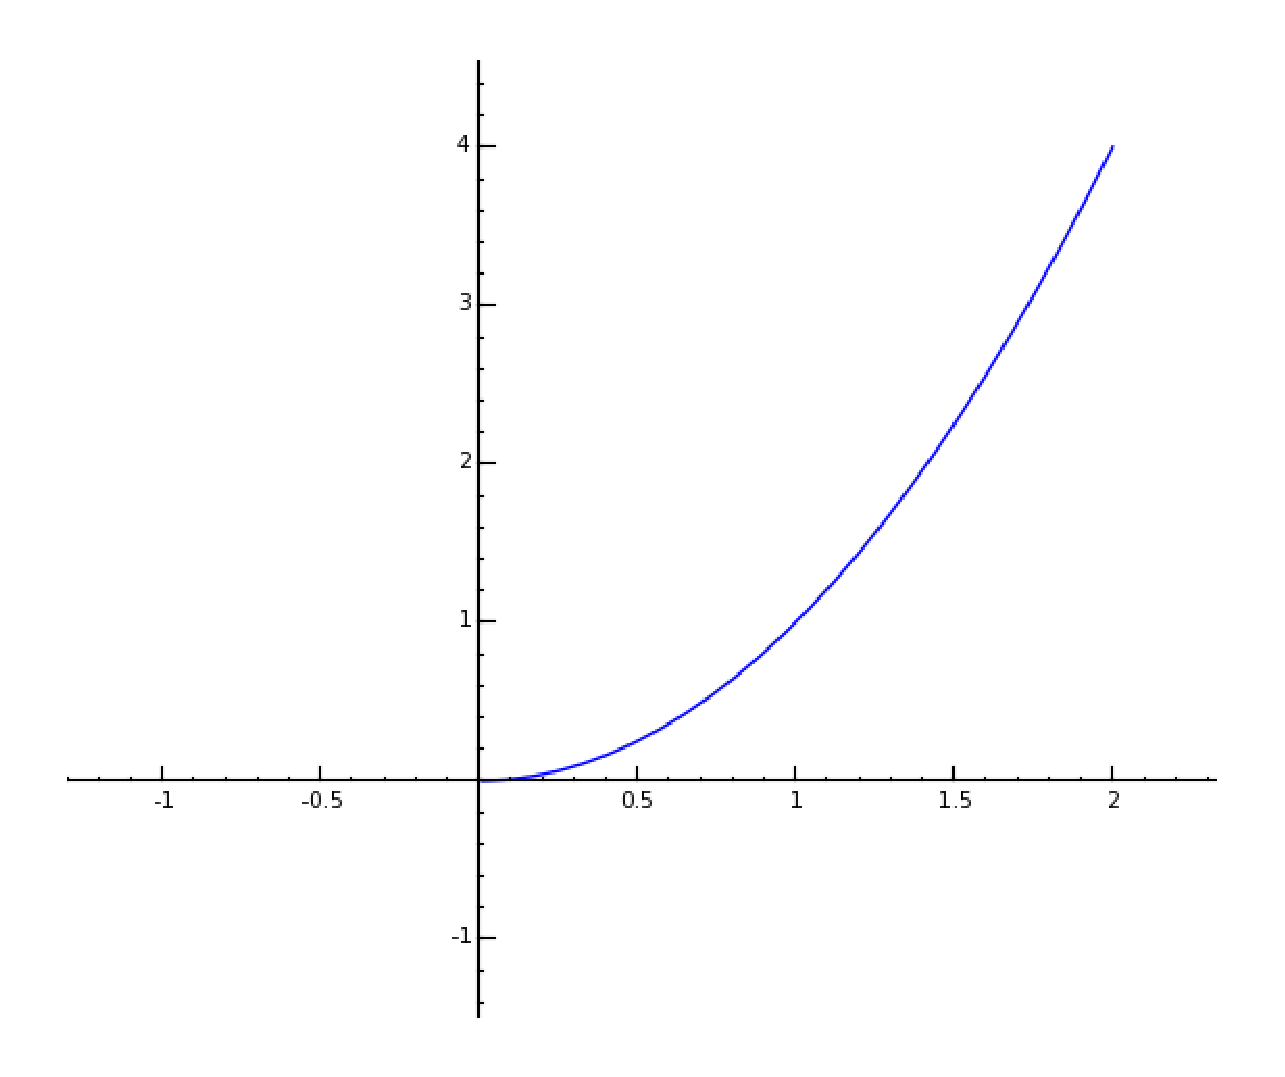
\includegraphics[height=5cm,width=5cm]{fcn-x2.eps}%
\lthtmlpictureZ
\lthtmlcheckvsize\clearpage}

{\newpage\clearpage
\lthtmlpictureA{tex2html_wrap46701}%
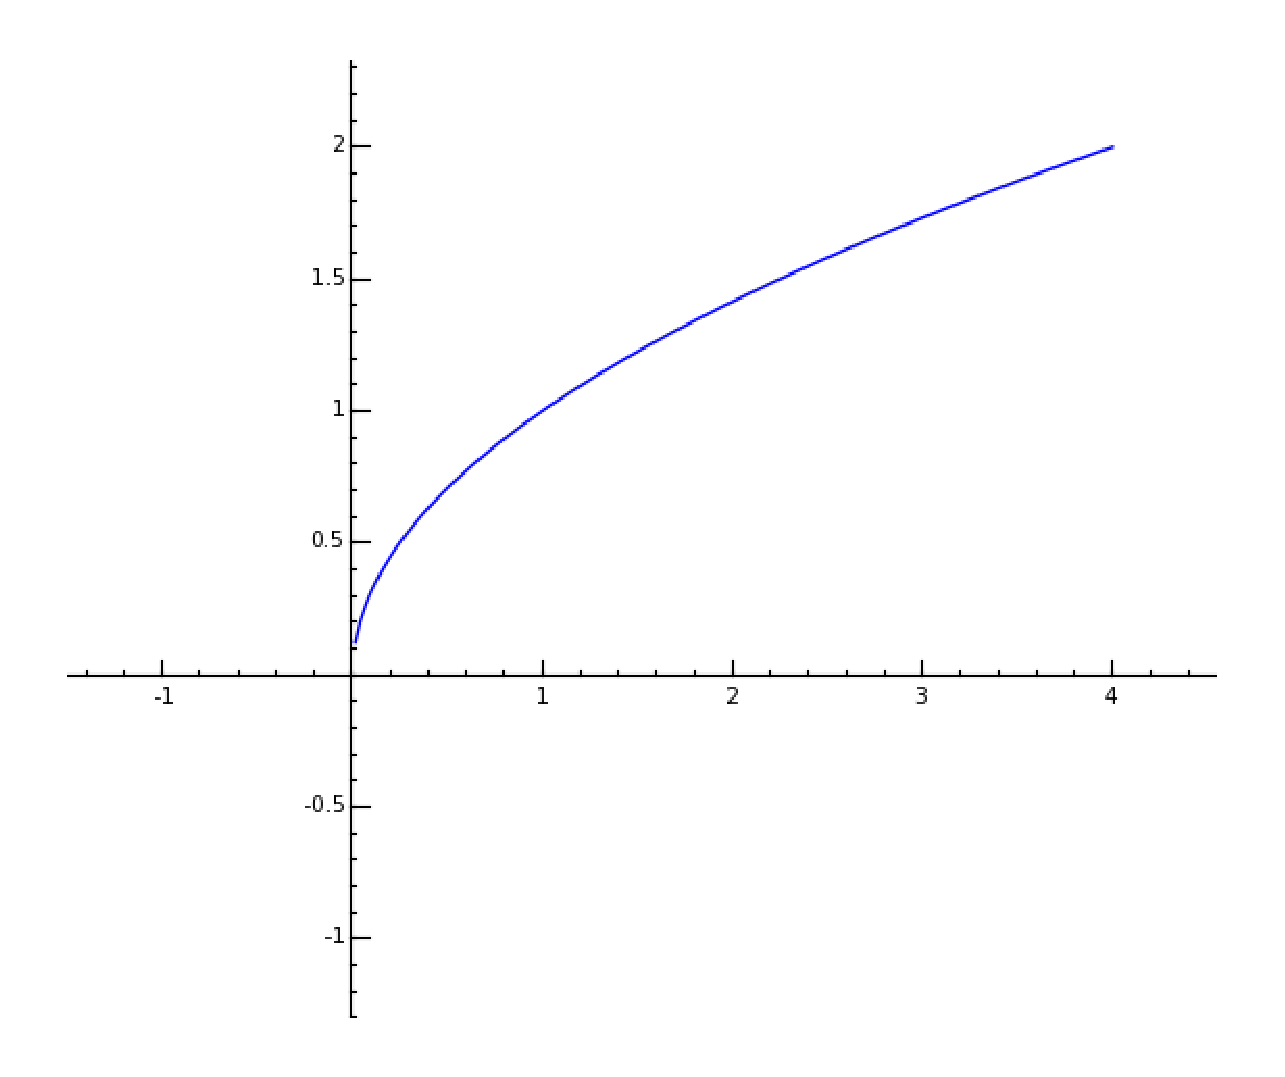
\includegraphics[height=5cm,width=5cm]{invfcn-x2.eps}%
\lthtmlpictureZ
\lthtmlcheckvsize\clearpage}

{\newpage\clearpage
\lthtmlinlinemathA{tex2html_wrap_inline46710}%
$ \tan(x)$%
\lthtmlinlinemathZ
\lthtmlcheckvsize\clearpage}

{\newpage\clearpage
\lthtmlinlinemathA{tex2html_wrap_inline46712}%
$ \arctan(x)$%
\lthtmlinlinemathZ
\lthtmlcheckvsize\clearpage}

{\newpage\clearpage
\lthtmlinlinemathA{tex2html_wrap_indisplay46714}%
$\displaystyle y = f(x)\  \ {\rm and}\  \  x = \phi(y)
$%
\lthtmlindisplaymathZ
\lthtmlcheckvsize\clearpage}

{\newpage\clearpage
\lthtmlinlinemathA{tex2html_wrap_inline46716}%
$ y + \Delta y 	= f(x + \Delta x)$%
\lthtmlinlinemathZ
\lthtmlcheckvsize\clearpage}

{\newpage\clearpage
\lthtmlinlinemathA{tex2html_wrap_inline46718}%
$ x + \Delta x =\phi(y + \Delta y)$%
\lthtmlinlinemathZ
\lthtmlcheckvsize\clearpage}

{\newpage\clearpage
\lthtmldisplayA{displaymath46720}%
\begin{displaymath}
\begin{array}{rlcrl}
y + \Delta y &	= f(x + \Delta x),  & \qquad & 	x + \Delta x &=	\phi (y + \Delta y)\\
  	y &= f(x),  & \qquad &	x &=\phi (y)\\
\Delta y &= f(x + \Delta x) - f(x), & \qquad &	\Delta x &= \phi(y + \Delta y) - \phi (y)\\
\end{array}
\end{displaymath}%
\lthtmldisplayZ
\lthtmlcheckvsize\clearpage}

{\newpage\clearpage
\lthtmlinlinemathA{tex2html_wrap_indisplay46722}%
$\displaystyle \frac{\Delta y}{\Delta x} = \frac{f(x + \Delta x) - f(x)}{\Delta x},
\qquad
\frac{\Delta x}{\Delta y} = \frac{\phi(y + \Delta y) - \phi(y)}{\Delta y}.
$%
\lthtmlindisplaymathZ
\lthtmlcheckvsize\clearpage}

{\newpage\clearpage
\lthtmlinlinemathA{tex2html_wrap_inline46724}%
$ \frac{\Delta y}{\Delta x} \cdot \frac{\Delta x}{\Delta y} 	= 1$%
\lthtmlinlinemathZ
\lthtmlcheckvsize\clearpage}

{\newpage\clearpage
\lthtmlinlinemathA{tex2html_wrap_inline46726}%
$ \frac{\Delta y}{\Delta x} 	= \frac{1}{\frac{\Delta x}{\Delta y}}$%
\lthtmlinlinemathZ
\lthtmlcheckvsize\clearpage}

{\newpage\clearpage
\lthtmlinlinemathA{tex2html_wrap_indisplay46728}%
$\displaystyle \frac{dy}{dx} 	= \frac{1}{\frac{dx}{dy}},$%
\lthtmlindisplaymathZ
\lthtmlcheckvsize\clearpage}

{\newpage\clearpage
\lthtmlinlinemathA{tex2html_wrap_indisplay46730}%
$\displaystyle f'(x) 	= \frac{1}{\phi'(y)}.
$%
\lthtmlindisplaymathZ
\lthtmlcheckvsize\clearpage}

\stepcounter{section}
{\newpage\clearpage
\lthtmlinlinemathA{tex2html_wrap_inline46739}%
$ y = log_av$%
\lthtmlinlinemathZ
\lthtmlcheckvsize\clearpage}

{\newpage\clearpage
\lthtmlinlinemathA{tex2html_wrap_inline46743}%
$ \  y + \Delta y 	= \log_a(v + \Delta v)$%
\lthtmlinlinemathZ
\lthtmlcheckvsize\clearpage}

{\newpage\clearpage
\lthtmlinlinemathA{tex2html_wrap_inline46747}%
$ \frac{\Delta y}{\Delta v} = \frac{\log_a(v + \Delta v) - \log_a v}{\Delta v}$%
\lthtmlinlinemathZ
\lthtmlcheckvsize\clearpage}

{\newpage\clearpage
\lthtmlinlinemathA{tex2html_wrap_inline46749}%
$ \frac{dy}{dx} = \frac{0}{0}$%
\lthtmlinlinemathZ
\lthtmlcheckvsize\clearpage}

{\newpage\clearpage
\lthtmldisplayA{displaymath46751}%
\begin{displaymath}
\begin{array}{ll}
 \Delta y &= \log_a(v + \Delta v) - \log_a v\\
 & = \log_a \left ( \frac{v + \Delta v}{v} \right )\\
& = \log_a \left ( 1 + \frac{\Delta v}{v} \right ).
\end{array}
\end{displaymath}%
\lthtmldisplayZ
\lthtmlcheckvsize\clearpage}

{\newpage\clearpage
\lthtmldisplayA{displaymath46753}%
\begin{displaymath}
\begin{array}{ll}
\frac{\Delta y}{\Delta x} &= \frac{1}{\Delta v} \log_a \left ( 1 + \frac{\Delta v}{v} \right ) \\
&= \log_a \left ( 1 + \frac{\Delta v}{v} \right )^{\frac{1}{\Delta v}}\\
 & 	= \frac{1}{v} \log_a \left ( 1 + \frac{\Delta v}{v} \right )^{\frac{v}{\Delta v}}.
\end{array}
\end{displaymath}%
\lthtmldisplayZ
\lthtmlcheckvsize\clearpage}

{\newpage\clearpage
\lthtmlinlinemathA{tex2html_wrap_inline46759}%
$ \frac{dy}{dv} 	= \frac{1}{v} \log_a e$%
\lthtmlinlinemathZ
\lthtmlcheckvsize\clearpage}

{\newpage\clearpage
\lthtmlinlinemathA{tex2html_wrap_inline46761}%
$ \Delta v \to 0$%
\lthtmlinlinemathZ
\lthtmlcheckvsize\clearpage}

{\newpage\clearpage
\lthtmlinlinemathA{tex2html_wrap_inline46763}%
$ \frac{\Delta v}{v} \to 0$%
\lthtmlinlinemathZ
\lthtmlcheckvsize\clearpage}

{\newpage\clearpage
\lthtmlinlinemathA{tex2html_wrap_inline46765}%
$ \lim_{\Delta v \to 0} \left ( 1 + \frac{\Delta v}{v} \right )^{\frac{v}{\Delta v}} = e$%
\lthtmlinlinemathZ
\lthtmlcheckvsize\clearpage}

{\newpage\clearpage
\lthtmlinlinemathA{tex2html_wrap_inline46767}%
$ x = \frac{\Delta v}{v}$%
\lthtmlinlinemathZ
\lthtmlcheckvsize\clearpage}

{\newpage\clearpage
\lthtmlinlinemathA{tex2html_wrap_indisplay46769}%
$\displaystyle \frac{dy}{dv} 	= \frac{d}{dv} \left ( \log_a v \right ) = \log_a e \cdot \frac{1}{v}.$%
\lthtmlindisplaymathZ
\lthtmlcheckvsize\clearpage}

{\newpage\clearpage
\lthtmlinlinemathA{tex2html_wrap_inline46775}%
$ \log_a v$%
\lthtmlinlinemathZ
\lthtmlcheckvsize\clearpage}

{\newpage\clearpage
\lthtmlinlinemathA{tex2html_wrap_indisplay46779}%
$\displaystyle \frac{dy}{dx} 	= \frac{dy}{dv} \cdot \frac{dv}{dx}.
$%
\lthtmlindisplaymathZ
\lthtmlcheckvsize\clearpage}

{\newpage\clearpage
\lthtmlinlinemathA{tex2html_wrap_inline46781}%
$ \frac{dy}{dv}$%
\lthtmlinlinemathZ
\lthtmlcheckvsize\clearpage}

{\newpage\clearpage
\lthtmlinlinemathA{tex2html_wrap_indisplay46783}%
$\displaystyle \frac{dy}{dx} 	= \log_a e \cdot \frac{1}{v} \cdot \frac{dv}{dx}.
$%
\lthtmlindisplaymathZ
\lthtmlcheckvsize\clearpage}

{\newpage\clearpage
\lthtmlinlinemathA{tex2html_wrap_inline46785}%
$ \frac{d}{dx} (\log_a x) 	= \log_s e \cdot \frac{\frac{dv}{dx}}{v}$%
\lthtmlinlinemathZ
\lthtmlcheckvsize\clearpage}

{\newpage\clearpage
\lthtmlinlinemathA{tex2html_wrap_inline46787}%
$ a = e$%
\lthtmlinlinemathZ
\lthtmlcheckvsize\clearpage}

{\newpage\clearpage
\lthtmlinlinemathA{tex2html_wrap_inline46789}%
$ \log_a e = log_e e = 1$%
\lthtmlinlinemathZ
\lthtmlcheckvsize\clearpage}

{\newpage\clearpage
\lthtmlinlinemathA{tex2html_wrap_inline46791}%
$ \frac{d}{dx} (\log v) 	= \frac{\frac{dv}{dx}}{v}$%
\lthtmlinlinemathZ
\lthtmlcheckvsize\clearpage}

{\newpage\clearpage
\lthtmlinlinemathA{tex2html_wrap_inline46799}%
$ = log_ae$%
\lthtmlinlinemathZ
\lthtmlcheckvsize\clearpage}

{\newpage\clearpage
\lthtmlinlinemathA{tex2html_wrap_inline46803}%
$ N$%
\lthtmlinlinemathZ
\lthtmlcheckvsize\clearpage}

{\newpage\clearpage
\lthtmlinlinemathA{tex2html_wrap_inline46807}%
$ \log_a N = \log_a e \cdot \log_e N = \frac{\log_e N}{\log_e a}.
$%
\lthtmlinlinemathZ
\lthtmlcheckvsize\clearpage}

{\newpage\clearpage
\lthtmlinlinemathA{tex2html_wrap_inline46809}%
$ 10$%
\lthtmlinlinemathZ
\lthtmlcheckvsize\clearpage}

{\newpage\clearpage
\lthtmlinlinemathA{tex2html_wrap_inline46811}%
$ \log_{10}e = .434294...$%
\lthtmlinlinemathZ
\lthtmlcheckvsize\clearpage}

\stepcounter{section}
{\newpage\clearpage
\lthtmlinlinemathA{tex2html_wrap_inline46814}%
$ y 	= a^v$%
\lthtmlinlinemathZ
\lthtmlcheckvsize\clearpage}

{\newpage\clearpage
\lthtmlinlinemathA{tex2html_wrap_inline46820}%
$ \log y = v \log a$%
\lthtmlinlinemathZ
\lthtmlcheckvsize\clearpage}

{\newpage\clearpage
\lthtmlinlinemathA{tex2html_wrap_inline46822}%
$ v 	= \frac{\log y}{\log a}	= \frac{1}{\log a} \cdot \log y$%
\lthtmlinlinemathZ
\lthtmlcheckvsize\clearpage}

{\newpage\clearpage
\lthtmlinlinemathA{tex2html_wrap_indisplay46826}%
$\displaystyle \frac{dv}{dy} 	= \frac{1}{\log a} \cdot \frac{1}{y};
$%
\lthtmlindisplaymathZ
\lthtmlcheckvsize\clearpage}

{\newpage\clearpage
\lthtmlinlinemathA{tex2html_wrap_inline46828}%
$ \frac{dy}{dv} 	= \log a \cdot y$%
\lthtmlinlinemathZ
\lthtmlcheckvsize\clearpage}

{\newpage\clearpage
\lthtmlinlinemathA{tex2html_wrap_indisplay46830}%
$\displaystyle \frac{dy}{dv} 	= \log a \cdot a^v.
$%
\lthtmlindisplaymathZ
\lthtmlcheckvsize\clearpage}

{\newpage\clearpage
\lthtmlinlinemathA{tex2html_wrap_inline46836}%
$ a^v$%
\lthtmlinlinemathZ
\lthtmlcheckvsize\clearpage}

{\newpage\clearpage
\lthtmlinlinemathA{tex2html_wrap_indisplay46844}%
$\displaystyle \frac{dy}{dx} 	= \log a \cdot a^v \cdot \frac{dv}{dx}.
$%
\lthtmlindisplaymathZ
\lthtmlcheckvsize\clearpage}

{\newpage\clearpage
\lthtmlinlinemathA{tex2html_wrap_inline46846}%
$ \frac{d}{dx} (a^v) 	= \log a \cdot a^v \cdot \frac{dv}{dx}$%
\lthtmlinlinemathZ
\lthtmlcheckvsize\clearpage}

{\newpage\clearpage
\lthtmlinlinemathA{tex2html_wrap_inline46850}%
$ \log a = \log e = 1$%
\lthtmlinlinemathZ
\lthtmlcheckvsize\clearpage}

{\newpage\clearpage
\lthtmlinlinemathA{tex2html_wrap_inline46852}%
$ \frac{d}{dx} (e^v) 	= e^v \frac{dv}{dx}$%
\lthtmlinlinemathZ
\lthtmlcheckvsize\clearpage}

\stepcounter{section}
{\newpage\clearpage
\lthtmlinlinemathA{tex2html_wrap_inline46859}%
$ y 	= u^v$%
\lthtmlinlinemathZ
\lthtmlcheckvsize\clearpage}

{\newpage\clearpage
\lthtmlinlinemathA{tex2html_wrap_inline46863}%
$ \log_e y= v \log_e u$%
\lthtmlinlinemathZ
\lthtmlcheckvsize\clearpage}

{\newpage\clearpage
\lthtmlinlinemathA{tex2html_wrap_inline46865}%
$ y 	= e^{v \log u}$%
\lthtmlinlinemathZ
\lthtmlcheckvsize\clearpage}

{\newpage\clearpage
\lthtmldisplayA{displaymath46867}%
\begin{displaymath}
\begin{array}{ll}
  	\frac{dy}{dx} &	= e^{v \log u} \frac{d}{dx} (v \log u)\\
  &	= e^{v \log u} \left ( \frac{v}{u} \frac{du}{dx} + \log u \frac{dv}{dx} \right ) \  \ {\rm by\  V}\\
  &	= u^v \left ( \frac{v}{u} \frac{du}{dx} + \log u \frac{dv}{dx} \right )
\end{array}
\end{displaymath}%
\lthtmldisplayZ
\lthtmlcheckvsize\clearpage}

{\newpage\clearpage
\lthtmlinlinemathA{tex2html_wrap_inline46869}%
$ \frac{d}{dx}(u^v) 	= vu^{v - 1}\frac{du}{dx} + \log u \cdot u^v \frac{dv}{dx}$%
\lthtmlinlinemathZ
\lthtmlcheckvsize\clearpage}

{\newpage\clearpage
\lthtmlinlinemathA{tex2html_wrap_inline46871}%
$ v = n$%
\lthtmlinlinemathZ
\lthtmlcheckvsize\clearpage}

{\newpage\clearpage
\lthtmlinlinemathA{tex2html_wrap_indisplay46873}%
$\displaystyle \frac{d}{dx}(u^n) = nu^{n - 1} \frac{du}{dx}.
$%
\lthtmlindisplaymathZ
\lthtmlcheckvsize\clearpage}

{\newpage\clearpage
\lthtmlinlinemathA{tex2html_wrap_inline46882}%
$ y = \log(x^2 + a)$%
\lthtmlinlinemathZ
\lthtmlcheckvsize\clearpage}

{\newpage\clearpage
\lthtmldisplayA{displaymath46884}%
\begin{displaymath}
\begin{array}{ll}
\frac{dy}{dx} 	&= \frac{\frac{d}{dx}(x^2 + a)}{x^2 + a} \  \ {\rm by\  VIIIa}\  (v = x^2 + a)\\
  	&= \frac{2x}{x^2 + a} .
\end{array}
\end{displaymath}%
\lthtmldisplayZ
\lthtmlcheckvsize\clearpage}

{\newpage\clearpage
\lthtmlinlinemathA{tex2html_wrap_inline46891}%
$ y = \log \sqrt{1 - x^2}$%
\lthtmlinlinemathZ
\lthtmlcheckvsize\clearpage}

{\newpage\clearpage
\lthtmldisplayA{displaymath46893}%
\begin{displaymath}
\begin{array}{ll}
	\frac{dy}{dx} 
&	= \frac{\frac{d}{dx}(1 - x^2)^{\frac{1}{2}}}{(1 - x^2)^{\frac{1}{2}}} \  \ {\rm by\  VIIIa}\\
&  	= \frac{\frac{1}{2} (1 - x^2)^{-\frac{1}{2}}(-2x)}{(1 - x^2)^{\frac{1}{2}}} \  \ {\rm by\  VI}\\
&  	= \frac{x}{x^2 - 1}.
\end{array}
\end{displaymath}%
\lthtmldisplayZ
\lthtmlcheckvsize\clearpage}

{\newpage\clearpage
\lthtmlinlinemathA{tex2html_wrap_inline46900}%
$ y = a^{3x^2}$%
\lthtmlinlinemathZ
\lthtmlcheckvsize\clearpage}

{\newpage\clearpage
\lthtmldisplayA{displaymath46902}%
\begin{displaymath}
\begin{array}{ll}
 	\frac{dy}{dx} &	= \log a \cdot a^{3x^2} \frac{d}{dx}(3 x^2) \  \ {\rm by\  IX}\\
  &	= 6x \log a \cdot a^{3x^2}.
\end{array}
\end{displaymath}%
\lthtmldisplayZ
\lthtmlcheckvsize\clearpage}

{\newpage\clearpage
\lthtmlinlinemathA{tex2html_wrap_inline46909}%
$ y = be^{c^2 + x^2}$%
\lthtmlinlinemathZ
\lthtmlcheckvsize\clearpage}

{\newpage\clearpage
\lthtmldisplayA{displaymath46911}%
\begin{displaymath}
\begin{array}{ll}
	\frac{dy}{dx} 
&=	b\frac{d}{dx} \left ( e^{c^2 + x^2} \right ) \  \ {\rm by\  IV}\\
&  	= be^{c^2 + x^2} \frac{d}{dx} (c^2 + x^2)  \  \ {\rm by\  IXa}\\
&  	= 2bxe^{c^2 + x^2}.
\end{array}
\end{displaymath}%
\lthtmldisplayZ
\lthtmlcheckvsize\clearpage}

{\newpage\clearpage
\lthtmlinlinemathA{tex2html_wrap_inline46918}%
$ y = x^{e^x}$%
\lthtmlinlinemathZ
\lthtmlcheckvsize\clearpage}

{\newpage\clearpage
\lthtmldisplayA{displaymath46920}%
\begin{displaymath}
\begin{array}{ll}
	\frac{dy}{dx} 
&	= e^x x^{e^x - 1} \frac{d}{dx} (x) + x^{e^x} \log x \frac{d}{dx} (e^x)  \  \ {\rm by\  X}\\
&  	= e^x x^{e^x - 1} + x^{e^x} \log x \cdot e^x\\
&  	= e^x x^{e^x} \left ( \frac{1}{x} + \log x \right ) 
\end{array}
\end{displaymath}%
\lthtmldisplayZ
\lthtmlcheckvsize\clearpage}

\stepcounter{section}
{\newpage\clearpage
\lthtmlinlinemathA{tex2html_wrap_inline46930}%
$ y 	= \frac{1}{2} \log (1 - x^2)$%
\lthtmlinlinemathZ
\lthtmlcheckvsize\clearpage}

{\newpage\clearpage
\lthtmldisplayA{displaymath46932}%
\begin{displaymath}
\begin{array}{ll}
	\frac{dy}{dx} 	
&= \frac{1}{2} \frac{\frac{d}{dx} (1 - x^2)}{1 - x^2}  \  \ {\rm by\  VIIIa}\\
&  	= \frac{1}{2} \cdot \frac{-2}{1 - x^2} = \frac{x}{x^2 - 1}. 
\end{array}
\end{displaymath}%
\lthtmldisplayZ
\lthtmlcheckvsize\clearpage}

{\newpage\clearpage
\lthtmlinlinemathA{tex2html_wrap_inline46939}%
$ y = \log \sqrt{\frac{1 + x^2}{1 - x^2}}$%
\lthtmlinlinemathZ
\lthtmlcheckvsize\clearpage}

{\newpage\clearpage
\lthtmldisplayA{displaymath46941}%
\begin{displaymath}
\begin{array}{ll}
  	y 	&= \frac{1}{2} [ \log (1 + x^2) - \log (1 - x^2) ]\\
\frac{dy}{dx} 	
&= \frac{1}{2} \left [ \frac{\frac{d}{dx} (1 + x^2)}{1 + x^2} 
- \frac{\frac{d}{dx} (1 - x^2)}{1 - x^2} \right ]   \  \ {\rm by\  VIIIa,\  etc.}\\
&  	= \frac{x}{1 + x^2} + \frac{x}{1 - x^2} = \frac{2x}{1 - x^4}. 
\end{array}
\end{displaymath}%
\lthtmldisplayZ
\lthtmlcheckvsize\clearpage}

{\newpage\clearpage
\lthtmlinlinemathA{tex2html_wrap_inline46950}%
$ \log y = e^x\log x$%
\lthtmlinlinemathZ
\lthtmlcheckvsize\clearpage}

{\newpage\clearpage
\lthtmldisplayA{displaymath46954}%
\begin{displaymath}
\begin{array}{ll}
\frac{\frac{dy}{dx}}{y} 
&	= e^x \frac{d}{dx} (\log x) + \log x \frac{d}{dx} (e^x)   \  \ {\rm by\  VIII\  and\  V}\\
&  	= e^x \cdot \frac{1}{x} + \log x \cdot e^x,
\end{array}
\end{displaymath}%
\lthtmldisplayZ
\lthtmlcheckvsize\clearpage}

{\newpage\clearpage
\lthtmlinlinemathA{tex2html_wrap_indisplay46956}%
$\displaystyle \frac{dy}{dx} 	= e^x \cdot y \left ( \frac{1}{x} \log x \right )
= e^x x^{e^x} \left ( \frac{1}{x} + \log x \right ).
$%
\lthtmlindisplaymathZ
\lthtmlcheckvsize\clearpage}

{\newpage\clearpage
\lthtmlinlinemathA{tex2html_wrap_inline46963}%
$ y = (4x^2 - 7)^{2 + \sqrt{x^2 - 5}}$%
\lthtmlinlinemathZ
\lthtmlcheckvsize\clearpage}

{\newpage\clearpage
\lthtmlinlinemathA{tex2html_wrap_indisplay46965}%
$\displaystyle \log y = (2 + \sqrt{x^2 - 5}) \log (4x^2 - 7).
$%
\lthtmlindisplaymathZ
\lthtmlcheckvsize\clearpage}

{\newpage\clearpage
\lthtmlinlinemathA{tex2html_wrap_indisplay46969}%
$\displaystyle \frac{1}{y} \frac{dy}{dx} 	= (2 + \sqrt{x^2 - 5}) \frac{8x}{4x^2 - 7} + \log(4x^2 - 7) \cdot \frac{x}{\sqrt{x^2 - 5}}.
$%
\lthtmlindisplaymathZ
\lthtmlcheckvsize\clearpage}

{\newpage\clearpage
\lthtmlinlinemathA{tex2html_wrap_indisplay46971}%
$\displaystyle \frac{dy}{dx} 	= x(4x^2 - 7)^{2 + \sqrt{x^2 - 5}} \left [ \frac{8(2 + \sqrt{x^2 - 5})}{4x^2 - 7} + \frac{\log (4x^2 - 7)}{\sqrt{x^2 - 5}} \right ]. 
$%
\lthtmlindisplaymathZ
\lthtmlcheckvsize\clearpage}

{\newpage\clearpage
\lthtmlinlinemathA{tex2html_wrap_inline46978}%
$ y = \sqrt{\frac{(x - 1)(x - 2)}{(x - 3)(x - 4)}}$%
\lthtmlinlinemathZ
\lthtmlcheckvsize\clearpage}

{\newpage\clearpage
\lthtmlinlinemathA{tex2html_wrap_indisplay46980}%
$\displaystyle \log y = \frac{1}{2} [\log (x -1) + \log (x - 2) - \log(x - 3) - \log(x - 4)].
$%
\lthtmlindisplaymathZ
\lthtmlcheckvsize\clearpage}

{\newpage\clearpage
\lthtmldisplayA{displaymath46984}%
\begin{displaymath}
\begin{array}{ll}
\frac{1}{y} \frac{dy}{dx} &= \frac{1}{2} \left [ \frac{1}{x - 1} + \frac{1}{x - 2} - \frac{1}{x - 3} - \frac{1}{x - 4} \right ]\\
&	= -\frac{2x^2 - 10x + 11}{(x - 1)(x - 2)(x - 3)(x - 4)},
\end{array}
\end{displaymath}%
\lthtmldisplayZ
\lthtmlcheckvsize\clearpage}

{\newpage\clearpage
\lthtmlinlinemathA{tex2html_wrap_indisplay46986}%
$\displaystyle \frac{dy}{dx} 	= -\frac{2x^2 - 10x - 11}{(x - 1)^{\frac{1}{2}} (x - 2)^{\frac{1}{2}} ( x - 3)^{\frac{3}{2}} (x - 4)^{\frac{3}{2}}}.
$%
\lthtmlindisplaymathZ
\lthtmlcheckvsize\clearpage}

\stepcounter{section}
{\newpage\clearpage
\lthtmlinlinemathA{tex2html_wrap_inline46991}%
$ y = \log(x + a)$%
\lthtmlinlinemathZ
\lthtmlcheckvsize\clearpage}

{\newpage\clearpage
\lthtmlinlinemathA{tex2html_wrap_inline46993}%
$ \frac{dy}{dx} = \frac{1}{x + a}$%
\lthtmlinlinemathZ
\lthtmlcheckvsize\clearpage}

{\newpage\clearpage
\lthtmlinlinemathA{tex2html_wrap_inline46995}%
$ y = \log(ax + b)$%
\lthtmlinlinemathZ
\lthtmlcheckvsize\clearpage}

{\newpage\clearpage
\lthtmlinlinemathA{tex2html_wrap_inline46997}%
$ \frac{dy}{dx} = \frac{a}{ax + b}$%
\lthtmlinlinemathZ
\lthtmlcheckvsize\clearpage}

{\newpage\clearpage
\lthtmlinlinemathA{tex2html_wrap_inline46999}%
$ y = \log \frac{1 + x^2}{1 - x^2}$%
\lthtmlinlinemathZ
\lthtmlcheckvsize\clearpage}

{\newpage\clearpage
\lthtmlinlinemathA{tex2html_wrap_inline47001}%
$ \frac{dy}{dx} = \frac{4x}{1 - x^4}$%
\lthtmlinlinemathZ
\lthtmlcheckvsize\clearpage}

{\newpage\clearpage
\lthtmlinlinemathA{tex2html_wrap_inline47003}%
$ y = \log(x^2 + x)$%
\lthtmlinlinemathZ
\lthtmlcheckvsize\clearpage}

{\newpage\clearpage
\lthtmlinlinemathA{tex2html_wrap_inline47005}%
$ y' = \frac{2x + 1}{x^2 + x}$%
\lthtmlinlinemathZ
\lthtmlcheckvsize\clearpage}

{\newpage\clearpage
\lthtmlinlinemathA{tex2html_wrap_inline47007}%
$ y = \log(x^3 - 2x + 5)$%
\lthtmlinlinemathZ
\lthtmlcheckvsize\clearpage}

{\newpage\clearpage
\lthtmlinlinemathA{tex2html_wrap_inline47009}%
$ y' = \frac{3x^2 - 2}{x^3 - 2x + 5}$%
\lthtmlinlinemathZ
\lthtmlcheckvsize\clearpage}

{\newpage\clearpage
\lthtmlinlinemathA{tex2html_wrap_inline47011}%
$ y = \log_a(2x + x^3)$%
\lthtmlinlinemathZ
\lthtmlcheckvsize\clearpage}

{\newpage\clearpage
\lthtmlinlinemathA{tex2html_wrap_inline47013}%
$ y' = \log_a e \cdot \frac{2 + 3x^2}{2x + x^3}$%
\lthtmlinlinemathZ
\lthtmlcheckvsize\clearpage}

{\newpage\clearpage
\lthtmlinlinemathA{tex2html_wrap_inline47015}%
$ y = x\log x$%
\lthtmlinlinemathZ
\lthtmlcheckvsize\clearpage}

{\newpage\clearpage
\lthtmlinlinemathA{tex2html_wrap_inline47017}%
$ y' = \log x + 1$%
\lthtmlinlinemathZ
\lthtmlcheckvsize\clearpage}

{\newpage\clearpage
\lthtmlinlinemathA{tex2html_wrap_inline47019}%
$ f(x) = \log (x^3)$%
\lthtmlinlinemathZ
\lthtmlcheckvsize\clearpage}

{\newpage\clearpage
\lthtmlinlinemathA{tex2html_wrap_inline47021}%
$ f'(x) = \frac{3}{x}$%
\lthtmlinlinemathZ
\lthtmlcheckvsize\clearpage}

{\newpage\clearpage
\lthtmlinlinemathA{tex2html_wrap_inline47023}%
$ f(x) = \log^3 x$%
\lthtmlinlinemathZ
\lthtmlcheckvsize\clearpage}

{\newpage\clearpage
\lthtmlinlinemathA{tex2html_wrap_inline47025}%
$ f'(x) = \frac{3 \log^2 x}{x}$%
\lthtmlinlinemathZ
\lthtmlcheckvsize\clearpage}

{\newpage\clearpage
\lthtmlinlinemathA{tex2html_wrap_inline47027}%
$ \log^3x = (\log x)^3$%
\lthtmlinlinemathZ
\lthtmlcheckvsize\clearpage}

{\newpage\clearpage
\lthtmlinlinemathA{tex2html_wrap_inline47029}%
$ v = \log x$%
\lthtmlinlinemathZ
\lthtmlcheckvsize\clearpage}

{\newpage\clearpage
\lthtmlinlinemathA{tex2html_wrap_inline47031}%
$ n = 3$%
\lthtmlinlinemathZ
\lthtmlcheckvsize\clearpage}

{\newpage\clearpage
\lthtmlinlinemathA{tex2html_wrap_inline47033}%
$ f(x) = \log \frac{a + x}{a - x}$%
\lthtmlinlinemathZ
\lthtmlcheckvsize\clearpage}

{\newpage\clearpage
\lthtmlinlinemathA{tex2html_wrap_inline47035}%
$ f'(x) = \frac{2a}{a^2 - x^2}$%
\lthtmlinlinemathZ
\lthtmlcheckvsize\clearpage}

{\newpage\clearpage
\lthtmlinlinemathA{tex2html_wrap_inline47037}%
$ f(x) = \log (x + \sqrt{1 + x^2})$%
\lthtmlinlinemathZ
\lthtmlcheckvsize\clearpage}

{\newpage\clearpage
\lthtmlinlinemathA{tex2html_wrap_inline47039}%
$ f'(x) = \frac{1}{\sqrt{1 + x^2}}$%
\lthtmlinlinemathZ
\lthtmlcheckvsize\clearpage}

{\newpage\clearpage
\lthtmlinlinemathA{tex2html_wrap_inline47041}%
$ \frac{d}{dx} e^{ax} = ae^{ax}$%
\lthtmlinlinemathZ
\lthtmlcheckvsize\clearpage}

{\newpage\clearpage
\lthtmlinlinemathA{tex2html_wrap_inline47043}%
$ \frac{d}{dx} e^{4x + 5} = 4e^{4x + 5}$%
\lthtmlinlinemathZ
\lthtmlcheckvsize\clearpage}

{\newpage\clearpage
\lthtmlinlinemathA{tex2html_wrap_inline47045}%
$ \frac{d}{dx} a^{3x} = 3a^{3x} \log a$%
\lthtmlinlinemathZ
\lthtmlcheckvsize\clearpage}

{\newpage\clearpage
\lthtmlinlinemathA{tex2html_wrap_inline47047}%
$ \frac{d}{dt} \log(3 - 2t^2) = \frac{4t}{2t^2 - 3}$%
\lthtmlinlinemathZ
\lthtmlcheckvsize\clearpage}

{\newpage\clearpage
\lthtmlinlinemathA{tex2html_wrap_inline47049}%
$ \frac{d}{dy} \log \frac{1 + y}{1 - y} = \frac{2}{1 - y^2}$%
\lthtmlinlinemathZ
\lthtmlcheckvsize\clearpage}

{\newpage\clearpage
\lthtmlinlinemathA{tex2html_wrap_inline47051}%
$ \frac{d}{dx}e^{b^2 + x^2} = 2xe^{b^2 + x^2}$%
\lthtmlinlinemathZ
\lthtmlcheckvsize\clearpage}

{\newpage\clearpage
\lthtmlinlinemathA{tex2html_wrap_inline47053}%
$ \frac{d}{d\theta} a^{\log a} = \frac{1}{\theta} a^{\log \theta} \log a$%
\lthtmlinlinemathZ
\lthtmlcheckvsize\clearpage}

{\newpage\clearpage
\lthtmlinlinemathA{tex2html_wrap_inline47055}%
$ \frac{d}{ds}b^{s^2} = 2x \log b \cdot b^{s^2}$%
\lthtmlinlinemathZ
\lthtmlcheckvsize\clearpage}

{\newpage\clearpage
\lthtmlinlinemathA{tex2html_wrap_inline47057}%
$ \frac{d}{dv} ae^{\sqrt{v}} = \frac{ae^{\sqrt{v}}}{2\sqrt{v}}$%
\lthtmlinlinemathZ
\lthtmlcheckvsize\clearpage}

{\newpage\clearpage
\lthtmlinlinemathA{tex2html_wrap_inline47059}%
$ \frac{d}{dx} a^{e^x} = \log a \cdot a^{e^x} \cdot e^x$%
\lthtmlinlinemathZ
\lthtmlcheckvsize\clearpage}

{\newpage\clearpage
\lthtmlinlinemathA{tex2html_wrap_inline47061}%
$ y = 7^{x^2 + 2x}$%
\lthtmlinlinemathZ
\lthtmlcheckvsize\clearpage}

{\newpage\clearpage
\lthtmlinlinemathA{tex2html_wrap_inline47063}%
$ y' = 2\log 7 \cdot (x + 1) 7^{x^2 + 2x}$%
\lthtmlinlinemathZ
\lthtmlcheckvsize\clearpage}

{\newpage\clearpage
\lthtmlinlinemathA{tex2html_wrap_inline47065}%
$ y = c^{a^2 - x^2}$%
\lthtmlinlinemathZ
\lthtmlcheckvsize\clearpage}

{\newpage\clearpage
\lthtmlinlinemathA{tex2html_wrap_inline47067}%
$ y' = -2x \log c \cdot c^{a^2 - x^2}$%
\lthtmlinlinemathZ
\lthtmlcheckvsize\clearpage}

{\newpage\clearpage
\lthtmlinlinemathA{tex2html_wrap_inline47069}%
$ y = \log \frac{e^x}{1 + e^x}$%
\lthtmlinlinemathZ
\lthtmlcheckvsize\clearpage}

{\newpage\clearpage
\lthtmlinlinemathA{tex2html_wrap_inline47071}%
$ \frac{dy}{dx} = \frac{1}{1 + e^x}$%
\lthtmlinlinemathZ
\lthtmlcheckvsize\clearpage}

{\newpage\clearpage
\lthtmlinlinemathA{tex2html_wrap_inline47073}%
$ \frac{d}{dx} \left [ e^x ( 1- x^2 \right ] = e^x (1 - 2x - x^2)$%
\lthtmlinlinemathZ
\lthtmlcheckvsize\clearpage}

{\newpage\clearpage
\lthtmlinlinemathA{tex2html_wrap_inline47075}%
$ \frac{d}{dx} \left ( \frac{e^x - 1}{e^x + 1} \right ) = \frac{2e^x}{(e^x + 1)^2}$%
\lthtmlinlinemathZ
\lthtmlcheckvsize\clearpage}

{\newpage\clearpage
\lthtmlinlinemathA{tex2html_wrap_inline47077}%
$ \frac{d}{dx} \left ( x^2 e^{ax} \right ) = xe^{ax}(ax + 2)$%
\lthtmlinlinemathZ
\lthtmlcheckvsize\clearpage}

{\newpage\clearpage
\lthtmlinlinemathA{tex2html_wrap_inline47079}%
$ y = \frac{a}{2} (e^{\frac{x}{a}} - e^{-\frac{x}{a}})$%
\lthtmlinlinemathZ
\lthtmlcheckvsize\clearpage}

{\newpage\clearpage
\lthtmlinlinemathA{tex2html_wrap_inline47081}%
$ \frac{dy}{dx} = \frac{1}{2} (e^{\frac{x}{a}} + e^{-\frac{x}{a}})$%
\lthtmlinlinemathZ
\lthtmlcheckvsize\clearpage}

{\newpage\clearpage
\lthtmlinlinemathA{tex2html_wrap_inline47083}%
$ y = \frac{e^x - e^{-x}}{e^x + e^{-x}}$%
\lthtmlinlinemathZ
\lthtmlcheckvsize\clearpage}

{\newpage\clearpage
\lthtmlinlinemathA{tex2html_wrap_inline47085}%
$ \frac{dy}{dx} = \frac{4}{(e^x + e^{-x}))^2}$%
\lthtmlinlinemathZ
\lthtmlcheckvsize\clearpage}

{\newpage\clearpage
\lthtmlinlinemathA{tex2html_wrap_inline47087}%
$ y = x^na^x$%
\lthtmlinlinemathZ
\lthtmlcheckvsize\clearpage}

{\newpage\clearpage
\lthtmlinlinemathA{tex2html_wrap_inline47089}%
$ y' = a^xx^{n - 1}(n + x\log a)$%
\lthtmlinlinemathZ
\lthtmlcheckvsize\clearpage}

{\newpage\clearpage
\lthtmlinlinemathA{tex2html_wrap_inline47091}%
$ y = x^x$%
\lthtmlinlinemathZ
\lthtmlcheckvsize\clearpage}

{\newpage\clearpage
\lthtmlinlinemathA{tex2html_wrap_inline47093}%
$ y' = x^x(\log x + 1)$%
\lthtmlinlinemathZ
\lthtmlcheckvsize\clearpage}

{\newpage\clearpage
\lthtmlinlinemathA{tex2html_wrap_inline47095}%
$ y = x^{\frac{1}{x}}$%
\lthtmlinlinemathZ
\lthtmlcheckvsize\clearpage}

{\newpage\clearpage
\lthtmlinlinemathA{tex2html_wrap_inline47097}%
$ y' = \frac{x^{\frac{1}{x}} (1 - \log x)}{x^2}$%
\lthtmlinlinemathZ
\lthtmlcheckvsize\clearpage}

{\newpage\clearpage
\lthtmlinlinemathA{tex2html_wrap_inline47099}%
$ y = x^{\log x}$%
\lthtmlinlinemathZ
\lthtmlcheckvsize\clearpage}

{\newpage\clearpage
\lthtmlinlinemathA{tex2html_wrap_inline47101}%
$ y' = \log (x^2) \cdot x^{\log x - 1}$%
\lthtmlinlinemathZ
\lthtmlcheckvsize\clearpage}

{\newpage\clearpage
\lthtmlinlinemathA{tex2html_wrap_inline47103}%
$ f(y) = \log y \cdot e^y$%
\lthtmlinlinemathZ
\lthtmlcheckvsize\clearpage}

{\newpage\clearpage
\lthtmlinlinemathA{tex2html_wrap_inline47105}%
$ f'(y) = e^y \left ( \log y + \frac{1}{y} \right )$%
\lthtmlinlinemathZ
\lthtmlcheckvsize\clearpage}

{\newpage\clearpage
\lthtmlinlinemathA{tex2html_wrap_inline47107}%
$ f(s) = \frac{\log s}{e^s}$%
\lthtmlinlinemathZ
\lthtmlcheckvsize\clearpage}

{\newpage\clearpage
\lthtmlinlinemathA{tex2html_wrap_inline47109}%
$ f'(s) = \frac{1 - s \log s}{s e^s}$%
\lthtmlinlinemathZ
\lthtmlcheckvsize\clearpage}

{\newpage\clearpage
\lthtmlinlinemathA{tex2html_wrap_inline47111}%
$ f(x) = \log(\log x)$%
\lthtmlinlinemathZ
\lthtmlcheckvsize\clearpage}

{\newpage\clearpage
\lthtmlinlinemathA{tex2html_wrap_inline47113}%
$ f'(x) = \frac{1}{x \log x}$%
\lthtmlinlinemathZ
\lthtmlcheckvsize\clearpage}

{\newpage\clearpage
\lthtmlinlinemathA{tex2html_wrap_inline47115}%
$ F(x) = \log^4(\log x)$%
\lthtmlinlinemathZ
\lthtmlcheckvsize\clearpage}

{\newpage\clearpage
\lthtmlinlinemathA{tex2html_wrap_inline47117}%
$ F'(x) = \frac{4 \log^3 (\log x)}{x \log x}$%
\lthtmlinlinemathZ
\lthtmlcheckvsize\clearpage}

{\newpage\clearpage
\lthtmlinlinemathA{tex2html_wrap_inline47119}%
$ \phi (x) = \log(\log^4x)$%
\lthtmlinlinemathZ
\lthtmlcheckvsize\clearpage}

{\newpage\clearpage
\lthtmlinlinemathA{tex2html_wrap_inline47121}%
$ \phi'(x) = \frac{4}{x \log x}$%
\lthtmlinlinemathZ
\lthtmlcheckvsize\clearpage}

{\newpage\clearpage
\lthtmlinlinemathA{tex2html_wrap_inline47123}%
$ \psi(y) = \log \sqrt{\frac{1 + y}{1 - y}}$%
\lthtmlinlinemathZ
\lthtmlcheckvsize\clearpage}

{\newpage\clearpage
\lthtmlinlinemathA{tex2html_wrap_inline47125}%
$ \psi'(y) = \frac{1}{1 - y^2}$%
\lthtmlinlinemathZ
\lthtmlcheckvsize\clearpage}

{\newpage\clearpage
\lthtmlinlinemathA{tex2html_wrap_inline47127}%
$ f(x) = \log \frac{\sqrt{x^2 + 1} - x}{\sqrt{x^1 + 1} + x}$%
\lthtmlinlinemathZ
\lthtmlcheckvsize\clearpage}

{\newpage\clearpage
\lthtmlinlinemathA{tex2html_wrap_inline47129}%
$ f'(x) = -\frac{2}{\sqrt{1 + x^2}}$%
\lthtmlinlinemathZ
\lthtmlcheckvsize\clearpage}

{\newpage\clearpage
\lthtmlinlinemathA{tex2html_wrap_inline47131}%
$ y = x^{\frac{1}{\log x}}$%
\lthtmlinlinemathZ
\lthtmlcheckvsize\clearpage}

{\newpage\clearpage
\lthtmlinlinemathA{tex2html_wrap_inline47133}%
$ \frac{dy}{dx} = 0$%
\lthtmlinlinemathZ
\lthtmlcheckvsize\clearpage}

{\newpage\clearpage
\lthtmlinlinemathA{tex2html_wrap_inline47135}%
$ y = e^{x^x}$%
\lthtmlinlinemathZ
\lthtmlcheckvsize\clearpage}

{\newpage\clearpage
\lthtmlinlinemathA{tex2html_wrap_inline47137}%
$ \frac{dy}{dx} = e^{x^x}(1 + \log x)x^x$%
\lthtmlinlinemathZ
\lthtmlcheckvsize\clearpage}

{\newpage\clearpage
\lthtmlinlinemathA{tex2html_wrap_inline47139}%
$ y = \frac{c^x}{x^x}$%
\lthtmlinlinemathZ
\lthtmlcheckvsize\clearpage}

{\newpage\clearpage
\lthtmlinlinemathA{tex2html_wrap_inline47141}%
$ \frac{dy}{dx} = \left ( \frac{c}{x} \right )^x \left ( \log \frac{c}{x} - 1 \right )$%
\lthtmlinlinemathZ
\lthtmlcheckvsize\clearpage}

{\newpage\clearpage
\lthtmlinlinemathA{tex2html_wrap_inline47143}%
$ y = \left ( \frac{x}{n} \right )^{nx}$%
\lthtmlinlinemathZ
\lthtmlcheckvsize\clearpage}

{\newpage\clearpage
\lthtmlinlinemathA{tex2html_wrap_inline47145}%
$ \frac{dy}{dx} = n \left ( \frac{x}{n} \right )^{nx} \left ( 1 + \log \frac{x}{n} \right )$%
\lthtmlinlinemathZ
\lthtmlcheckvsize\clearpage}

{\newpage\clearpage
\lthtmlinlinemathA{tex2html_wrap_inline47147}%
$ w = v^{e^v}$%
\lthtmlinlinemathZ
\lthtmlcheckvsize\clearpage}

{\newpage\clearpage
\lthtmlinlinemathA{tex2html_wrap_inline47149}%
$ \frac{dw}{dv} = v^{e^v} e^v \left ( \frac{1 + v \log v}{v} \right )$%
\lthtmlinlinemathZ
\lthtmlcheckvsize\clearpage}

{\newpage\clearpage
\lthtmlinlinemathA{tex2html_wrap_inline47151}%
$ z = \left ( \frac{a}{t} \right )^t$%
\lthtmlinlinemathZ
\lthtmlcheckvsize\clearpage}

{\newpage\clearpage
\lthtmlinlinemathA{tex2html_wrap_inline47153}%
$ \frac{dz}{dt} 
= \left ( \frac{a}{t} \right )^t (\log a - \log t - 1)$%
\lthtmlinlinemathZ
\lthtmlcheckvsize\clearpage}

{\newpage\clearpage
\lthtmlinlinemathA{tex2html_wrap_inline47155}%
$ y = x^{x^n}$%
\lthtmlinlinemathZ
\lthtmlcheckvsize\clearpage}

{\newpage\clearpage
\lthtmlinlinemathA{tex2html_wrap_inline47157}%
$ \frac{dy}{dx} = x^{x^n + n - 1}(n \log x + 1)$%
\lthtmlinlinemathZ
\lthtmlcheckvsize\clearpage}

{\newpage\clearpage
\lthtmlinlinemathA{tex2html_wrap_inline47159}%
$ y = x^{x^x}$%
\lthtmlinlinemathZ
\lthtmlcheckvsize\clearpage}

{\newpage\clearpage
\lthtmlinlinemathA{tex2html_wrap_inline47161}%
$ \frac{dy}{dx} = x^{x^x} x^x \left ( \log x + \log^2 x + \frac{1}{x} \right )$%
\lthtmlinlinemathZ
\lthtmlcheckvsize\clearpage}

{\newpage\clearpage
\lthtmlinlinemathA{tex2html_wrap_inline47163}%
$ y = a^{\frac{1}{\sqrt{a^2 - x^2}}}$%
\lthtmlinlinemathZ
\lthtmlcheckvsize\clearpage}

{\newpage\clearpage
\lthtmlinlinemathA{tex2html_wrap_inline47165}%
$ \frac{dy}{dx} = \frac{xy \log a}{(a^2 - x^2)^{\frac{3}{2}}}$%
\lthtmlinlinemathZ
\lthtmlcheckvsize\clearpage}

{\newpage\clearpage
\lthtmldisplayA{displaymath47167}%
\begin{displaymath}
\begin{array}{lll}
(a)\  \  \frac{d}{dx} x^2 \log x &  	(f)\  \  \frac{d}{dx} e^x \log x &  	(k)\  \  \frac{d}{dx} \log (a^x + b^x) \\
(b)\  \  \frac{d}{dx} (e^{2x} - 1)^4 &  	(g)\  \  \frac{d}{dx} x^3 3^x &	(l)\  \  \frac{d}{dx} \log_10 (x^2 + 5x)\\
(c)\  \  \frac{d}{dx} \log \frac{3x + 1}{x + 3} &  	(h)\  \  \frac{d}{dx} \frac{1}{x \log x} &  	(m)\  \  \frac{d}{dx} \frac{2 + x^2}{e^{3x}}\\
(d)\  \  \frac{d}{dx} \log \frac{1 - x^2}{\sqrt{1 + x}} &  	(i)\  \  \frac{d}{dx} \log x^3 \sqrt{1 + x^2} &  	(n)\  \  \frac{d}{dx} (x^2 + a^2) e^{x^2 + a^2}\\
(e)\  \  \frac{d}{dx} x^{\sqrt{x}} &  	(j)\  \  \frac{d}{dx} \left ( \frac{1}{x} \right )^x &  	(o)\  \  \frac{d}{dx} (x^2 + 4)^x.
\end{array}
\end{displaymath}%
\lthtmldisplayZ
\lthtmlcheckvsize\clearpage}

{\newpage\clearpage
\lthtmlinlinemathA{tex2html_wrap_inline47169}%
$ y = \frac{(x + 1)^2}{(x + 2)^3 (x + 3)^4}$%
\lthtmlinlinemathZ
\lthtmlcheckvsize\clearpage}

{\newpage\clearpage
\lthtmlinlinemathA{tex2html_wrap_inline47171}%
$ \frac{dy}{dx} = -\frac{(x + 1)(5x^2 + 14x + 5)}{(x + 2)^4 (x + 3)^5}$%
\lthtmlinlinemathZ
\lthtmlcheckvsize\clearpage}

{\newpage\clearpage
\lthtmlinlinemathA{tex2html_wrap_inline47173}%
$ y = \frac{((x - 1)^{\frac{5}{2}}}{(x - 2)^{\frac{3}{4}}(x - 3)^{\frac{7}{3}}}$%
\lthtmlinlinemathZ
\lthtmlcheckvsize\clearpage}

{\newpage\clearpage
\lthtmlinlinemathA{tex2html_wrap_inline47175}%
$ \frac{dy}{dx} 
= -\frac{(x - 1)^{\frac{3}{2}}(7x^2 + 30x - 97)}{12(x - 2)^{\frac{7}{4}}(x - 3)^{\frac{10}{3}}}$%
\lthtmlinlinemathZ
\lthtmlcheckvsize\clearpage}

{\newpage\clearpage
\lthtmlinlinemathA{tex2html_wrap_inline47177}%
$ y = x \sqrt{1 - x} (1 + x)$%
\lthtmlinlinemathZ
\lthtmlcheckvsize\clearpage}

{\newpage\clearpage
\lthtmlinlinemathA{tex2html_wrap_inline47179}%
$ \frac{dy}{dx} = \frac{2 + x - 5x^2}{2\sqrt{1 - x}}$%
\lthtmlinlinemathZ
\lthtmlcheckvsize\clearpage}

{\newpage\clearpage
\lthtmlinlinemathA{tex2html_wrap_inline47181}%
$ y = \frac{x(1 + x^2)}{\sqrt{1 - x^2}}$%
\lthtmlinlinemathZ
\lthtmlcheckvsize\clearpage}

{\newpage\clearpage
\lthtmlinlinemathA{tex2html_wrap_inline47183}%
$ \frac{dy}{dx} = \frac{1 + 3x^2 - 2x^4}{(1 - x^2}^{\frac{3}{2}}$%
\lthtmlinlinemathZ
\lthtmlcheckvsize\clearpage}

{\newpage\clearpage
\lthtmlinlinemathA{tex2html_wrap_inline47185}%
$ y = x^5(a + 3x)^3(a - 2x)^2$%
\lthtmlinlinemathZ
\lthtmlcheckvsize\clearpage}

{\newpage\clearpage
\lthtmlinlinemathA{tex2html_wrap_inline47187}%
$ \frac{dy}{dx} = 5x^4(a + 3x)^2(a - 2x)(a^2 + 2ax - 12x^2)$%
\lthtmlinlinemathZ
\lthtmlcheckvsize\clearpage}

\stepcounter{section}
{\newpage\clearpage
\lthtmlinlinemathA{tex2html_wrap_inline47190}%
$ \sin v$%
\lthtmlinlinemathZ
\lthtmlcheckvsize\clearpage}

{\newpage\clearpage
\lthtmlinlinemathA{tex2html_wrap_inline47192}%
$ y 	= \sin v$%
\lthtmlinlinemathZ
\lthtmlcheckvsize\clearpage}

{\newpage\clearpage
\lthtmlinlinemathA{tex2html_wrap_inline47196}%
$ y + \Delta y 	= \sin(v + \Delta v)$%
\lthtmlinlinemathZ
\lthtmlcheckvsize\clearpage}

{\newpage\clearpage
\lthtmlinlinemathA{tex2html_wrap_inline47200}%
$ \frac{\Delta y}{\Delta v} = \frac{\sin(v + \Delta v) - \sin v}{\Delta v}$%
\lthtmlinlinemathZ
\lthtmlcheckvsize\clearpage}

{\newpage\clearpage
\lthtmlinlinemathA{tex2html_wrap_inline47202}%
$ \frac{dy}{dv} = \frac{0}{0}$%
\lthtmlinlinemathZ
\lthtmlcheckvsize\clearpage}

{\newpage\clearpage
\lthtmlinlinemathA{tex2html_wrap_inline47206}%
$ A 	= v + \Delta v$%
\lthtmlinlinemathZ
\lthtmlcheckvsize\clearpage}

{\newpage\clearpage
\lthtmlinlinemathA{tex2html_wrap_inline47208}%
$ B 	= v$%
\lthtmlinlinemathZ
\lthtmlcheckvsize\clearpage}

{\newpage\clearpage
\lthtmlinlinemathA{tex2html_wrap_inline47210}%
$ A + B 	= 2v + \Delta v$%
\lthtmlinlinemathZ
\lthtmlcheckvsize\clearpage}

{\newpage\clearpage
\lthtmlinlinemathA{tex2html_wrap_inline47212}%
$ A - B 	= \Delta v$%
\lthtmlinlinemathZ
\lthtmlcheckvsize\clearpage}

{\newpage\clearpage
\lthtmlinlinemathA{tex2html_wrap_inline47214}%
$ \frac{1}{2}(A + B) 	= v + \frac{\Delta v}{2}$%
\lthtmlinlinemathZ
\lthtmlcheckvsize\clearpage}

{\newpage\clearpage
\lthtmlinlinemathA{tex2html_wrap_inline47216}%
$ \frac{1}{2}(A - B) 	= \frac{\Delta v}{2}$%
\lthtmlinlinemathZ
\lthtmlcheckvsize\clearpage}

{\newpage\clearpage
\lthtmlinlinemathA{tex2html_wrap_inline47222}%
$ \frac{1}{2}(A + B)$%
\lthtmlinlinemathZ
\lthtmlcheckvsize\clearpage}

{\newpage\clearpage
\lthtmlinlinemathA{tex2html_wrap_inline47224}%
$ \frac{1}{2}(A - B)$%
\lthtmlinlinemathZ
\lthtmlcheckvsize\clearpage}

{\newpage\clearpage
\lthtmlinlinemathA{tex2html_wrap_inline47230}%
$ \sin A - \sin B 	= 2 \cos \frac{1}{2} (A + B) \sin \frac{1}{2} (A - B),
$%
\lthtmlinlinemathZ
\lthtmlcheckvsize\clearpage}

{\newpage\clearpage
\lthtmlinlinemathA{tex2html_wrap_inline47232}%
$ \sin (v + \Delta v) - \sin v 	= 2 \cos \left ( v + \frac{\Delta v}{2} \right ) \sin \frac{\Delta v}{2}.
$%
\lthtmlinlinemathZ
\lthtmlcheckvsize\clearpage}

{\newpage\clearpage
\lthtmlinlinemathA{tex2html_wrap_indisplay47234}%
$\displaystyle \Delta y 	= \sin(v + \Delta v) - \sin v
= 2 \cos \left ( v + \frac{\Delta v}{2} \right ) \cdot \sin \frac{\Delta v}{2}.
$%
\lthtmlindisplaymathZ
\lthtmlcheckvsize\clearpage}

{\newpage\clearpage
\lthtmlinlinemathA{tex2html_wrap_indisplay47236}%
$\displaystyle \frac{\Delta y}{\Delta v} 
= \cos \left ( v + \frac{\Delta v}{2} \right ) \left ( \frac{\sin \frac{\Delta v}{2}}{\frac{\Delta v}{2}} \right ).
$%
\lthtmlindisplaymathZ
\lthtmlcheckvsize\clearpage}

{\newpage\clearpage
\lthtmlinlinemathA{tex2html_wrap_inline47238}%
$ \frac{dy}{dx} 	= \cos v$%
\lthtmlinlinemathZ
\lthtmlcheckvsize\clearpage}

{\newpage\clearpage
\lthtmlinlinemathA{tex2html_wrap_inline47240}%
$ \lim_{\Delta v \to 0} \left ( \frac{\sin \frac{\Delta v}{2}}{\frac{\Delta v}{2}} \right ) = 1$%
\lthtmlinlinemathZ
\lthtmlcheckvsize\clearpage}

{\newpage\clearpage
\lthtmlinlinemathA{tex2html_wrap_inline47242}%
$ \lim_{\Delta v \to 0} \cos \left ( v + \frac{\Delta v}{2} \right ) = \cos v$%
\lthtmlinlinemathZ
\lthtmlcheckvsize\clearpage}

{\newpage\clearpage
\lthtmlinlinemathA{tex2html_wrap_inline47256}%
$ \frac{dy}{dx} 	= \cos v \frac{dv}{dx}$%
\lthtmlinlinemathZ
\lthtmlcheckvsize\clearpage}

{\newpage\clearpage
\lthtmlinlinemathA{tex2html_wrap_indisplay47258}%
$\displaystyle \frac{d}{dx} (\sin v) 	= \cos v \frac{dv}{dx}
$%
\lthtmlindisplaymathZ
\lthtmlcheckvsize\clearpage}

\stepcounter{section}
{\newpage\clearpage
\lthtmlinlinemathA{tex2html_wrap_inline47261}%
$ \cos v$%
\lthtmlinlinemathZ
\lthtmlcheckvsize\clearpage}

{\newpage\clearpage
\lthtmlinlinemathA{tex2html_wrap_inline47263}%
$ y 	= \cos v$%
\lthtmlinlinemathZ
\lthtmlcheckvsize\clearpage}

{\newpage\clearpage
\lthtmlinlinemathA{tex2html_wrap_indisplay47265}%
$\displaystyle y 	= \sin \left ( \frac{\pi}{2} - v \right ).
$%
\lthtmlindisplaymathZ
\lthtmlcheckvsize\clearpage}

{\newpage\clearpage
\lthtmldisplayA{displaymath47267}%
\begin{displaymath}
\begin{array}{ll}
  \frac{dy}{dx} 
& = \cos \left ( \frac{\pi}{2} - v \right ) \frac{d}{dx} \left ( \frac{\pi}{2} - v \right )\\
& = \cos \left ( \frac{\pi}{2} - v \right ) \left ( -\frac{dv}{dx} \right )\\
& = -\sin x \frac{dv}{dx}.
\end{array}
\end{displaymath}%
\lthtmldisplayZ
\lthtmlcheckvsize\clearpage}

{\newpage\clearpage
\lthtmlinlinemathA{tex2html_wrap_inline47269}%
$ \cos \left ( \frac{\pi}{2} \right ) = \sin v$%
\lthtmlinlinemathZ
\lthtmlcheckvsize\clearpage}

{\newpage\clearpage
\lthtmlinlinemathA{tex2html_wrap_indisplay47271}%
$\displaystyle \frac{d}{dx} (\cos v) 	= -\sin v \frac{dv}{dx},
$%
\lthtmlindisplaymathZ
\lthtmlcheckvsize\clearpage}

\stepcounter{section}
{\newpage\clearpage
\lthtmlinlinemathA{tex2html_wrap_inline47274}%
$ \tan v$%
\lthtmlinlinemathZ
\lthtmlcheckvsize\clearpage}

{\newpage\clearpage
\lthtmlinlinemathA{tex2html_wrap_inline47276}%
$ y 	= \tan v$%
\lthtmlinlinemathZ
\lthtmlcheckvsize\clearpage}

{\newpage\clearpage
\lthtmldisplayA{displaymath47278}%
\begin{displaymath}
\begin{array}{ll}
  	\frac{dy}{dx}
& 	= \frac{\cos v \frac{d}{dx}(\sin v) - \sin v \frac{d}{dx}(\cos v)}{\cos^2 v}\\
 & 	= \frac{\cos^2 v \frac{dv}{dx} + \sin^2 v \frac{dv}{dx}}{\cos^2 v}\\
 & 	= \frac{\frac{dv}{dx}}{\cos^2 v} = \sec^2 v \frac{dv}{dx}.
\end{array}
\end{displaymath}%
\lthtmldisplayZ
\lthtmlcheckvsize\clearpage}

{\newpage\clearpage
\lthtmlinlinemathA{tex2html_wrap_indisplay47280}%
$\displaystyle \frac{d}{dx}(\tan x) 	= \sec^2 v \frac{dv}{dx},
$%
\lthtmlindisplaymathZ
\lthtmlcheckvsize\clearpage}

\stepcounter{section}
{\newpage\clearpage
\lthtmlinlinemathA{tex2html_wrap_inline47283}%
$ \cot v$%
\lthtmlinlinemathZ
\lthtmlcheckvsize\clearpage}

{\newpage\clearpage
\lthtmlinlinemathA{tex2html_wrap_inline47285}%
$ y 	= \cot v$%
\lthtmlinlinemathZ
\lthtmlcheckvsize\clearpage}

{\newpage\clearpage
\lthtmlinlinemathA{tex2html_wrap_inline47287}%
$ y 	= \frac{1}{\tan v}$%
\lthtmlinlinemathZ
\lthtmlcheckvsize\clearpage}

{\newpage\clearpage
\lthtmldisplayA{displaymath47289}%
\begin{displaymath}
\begin{array}{ll}
  	\frac{dy}{dx}
& 	= - \frac{\frac{d}{dx}(\tan v)}{\tan^2 v}\\
&  	= -\frac{\sec^2 \frac{dv}{dx}}{\tan^2 v} \\
& = -\csc^2 v \frac{dv}{dx}.
\end{array}
\end{displaymath}%
\lthtmldisplayZ
\lthtmlcheckvsize\clearpage}

{\newpage\clearpage
\lthtmlinlinemathA{tex2html_wrap_indisplay47291}%
$\displaystyle \frac{d}{dx}(\cot v) 	= -\csc^2 v \frac{dv}{dx}
$%
\lthtmlindisplaymathZ
\lthtmlcheckvsize\clearpage}

\stepcounter{section}
{\newpage\clearpage
\lthtmlinlinemathA{tex2html_wrap_inline47294}%
$ \sec v$%
\lthtmlinlinemathZ
\lthtmlcheckvsize\clearpage}

{\newpage\clearpage
\lthtmlinlinemathA{tex2html_wrap_inline47296}%
$ y = \sec v$%
\lthtmlinlinemathZ
\lthtmlcheckvsize\clearpage}

{\newpage\clearpage
\lthtmlinlinemathA{tex2html_wrap_inline47298}%
$ y 	= \frac{1}{\cos v}$%
\lthtmlinlinemathZ
\lthtmlcheckvsize\clearpage}

{\newpage\clearpage
\lthtmldisplayA{displaymath47300}%
\begin{displaymath}
\begin{array}{ll}
\frac{dy}{dx} 
&	= -\frac{\frac{d}{dx}(\cos v)}{\cos^2 v}\\
&  	=\frac{\sin v \frac{dv}{dx}}{\cos^2 v}\\
&  	= \frac{1}{\cos v} \frac{\sin v}{\cos v} \frac{dv}{dx}\\
&  	= \sec v \tan v \frac{dv}{dx}.
\end{array}
\end{displaymath}%
\lthtmldisplayZ
\lthtmlcheckvsize\clearpage}

{\newpage\clearpage
\lthtmlinlinemathA{tex2html_wrap_indisplay47302}%
$\displaystyle \frac{d}{dx}(\sec v) 	= \sec v \tan v \frac{dv}{dx}
$%
\lthtmlindisplaymathZ
\lthtmlcheckvsize\clearpage}

\stepcounter{section}
{\newpage\clearpage
\lthtmlinlinemathA{tex2html_wrap_inline47305}%
$ \csc\, v$%
\lthtmlinlinemathZ
\lthtmlcheckvsize\clearpage}

{\newpage\clearpage
\lthtmlinlinemathA{tex2html_wrap_inline47307}%
$ y 	= \csc\, v$%
\lthtmlinlinemathZ
\lthtmlcheckvsize\clearpage}

{\newpage\clearpage
\lthtmlinlinemathA{tex2html_wrap_indisplay47309}%
$\displaystyle y 	= \frac{1}{\sin v}.
$%
\lthtmlindisplaymathZ
\lthtmlcheckvsize\clearpage}

{\newpage\clearpage
\lthtmldisplayA{displaymath47311}%
\begin{displaymath}
\begin{array}{ll}
\frac{dy}{dx} 
&	= -\frac{\frac{d}{dx}(\sin v)}{\sin^2 v}\\
 & 	= -\frac{\cos v \frac{dv}{dx}}{\sin^2 v}\\
  &	= -\csc v \cot v \frac{dv}{dx}.
\end{array}
\end{displaymath}%
\lthtmldisplayZ
\lthtmlcheckvsize\clearpage}

{\newpage\clearpage
\lthtmlinlinemathA{tex2html_wrap_indisplay47313}%
$\displaystyle \frac{d}{dx}(\csc v) 	= - \csc v \cot v \frac{dv}{dx}
$%
\lthtmlindisplaymathZ
\lthtmlcheckvsize\clearpage}

\stepcounter{section}
{\newpage\clearpage
\lthtmlinlinemathA{tex2html_wrap_inline47316}%
$ {\rm vers}\, v$%
\lthtmlinlinemathZ
\lthtmlcheckvsize\clearpage}

{\newpage\clearpage
\lthtmlinlinemathA{tex2html_wrap_inline47318}%
$ y 	= {\rm vers}\  v$%
\lthtmlinlinemathZ
\lthtmlcheckvsize\clearpage}

{\newpage\clearpage
\lthtmlinlinemathA{tex2html_wrap_indisplay47320}%
$\displaystyle \  y 	= 1 - \cos v\  .
$%
\lthtmlindisplaymathZ
\lthtmlcheckvsize\clearpage}

{\newpage\clearpage
\lthtmlinlinemathA{tex2html_wrap_inline47322}%
$ \frac{dy}{dx} 	= \sin v \frac{dv}{dx}$%
\lthtmlinlinemathZ
\lthtmlcheckvsize\clearpage}

{\newpage\clearpage
\lthtmlinlinemathA{tex2html_wrap_inline47324}%
$ \frac{d}{dx}({\rm vers}\, v) 	= \sin v \frac{dv}{dx}$%
\lthtmlinlinemathZ
\lthtmlcheckvsize\clearpage}

\stepcounter{section}
{\newpage\clearpage
\lthtmlinlinemathA{tex2html_wrap_inline47329}%
$ \frac{d}{dx}(uv) 	= u \frac{dv}{dx} + v \frac{du}{dx}.  $%
\lthtmlinlinemathZ
\lthtmlcheckvsize\clearpage}

{\newpage\clearpage
\lthtmlinlinemathA{tex2html_wrap_inline47331}%
$ \frac{d}{dx} \left ( \frac{u}{v} \right ) 	= \frac{v \frac{du}{dx} - u \frac{dv}{dx}}{v^2}.  $%
\lthtmlinlinemathZ
\lthtmlcheckvsize\clearpage}

{\newpage\clearpage
\lthtmlinlinemathA{tex2html_wrap_inline47333}%
$ \frac{d}{dx}(\log_a v) 	= \log_a e \frac{\frac{dv}{dx}}{v}. $%
\lthtmlinlinemathZ
\lthtmlcheckvsize\clearpage}

{\newpage\clearpage
\lthtmlinlinemathA{tex2html_wrap_inline47337}%
$ \frac{dy}{dx} 	= \frac{dy}{dv} \cdot \frac{dv}{dx}.  $%
\lthtmlinlinemathZ
\lthtmlcheckvsize\clearpage}

{\newpage\clearpage
\lthtmlinlinemathA{tex2html_wrap_inline47339}%
$ \frac{dy}{dx} 	= \frac{1}{\frac{dx}{dy}}.  $%
\lthtmlinlinemathZ
\lthtmlcheckvsize\clearpage}

{\newpage\clearpage
\lthtmlinlinemathA{tex2html_wrap_indisplay47362}%

% latex2html id marker 47362
$\displaystyle \lim_{v \to 0} \frac{\sin v}{1} 	= 1\  \ \  \ \  \ {\rm by\  \S \ref{sec:22}},% § 22, p. 21
$%
\lthtmlindisplaymathZ
\lthtmlcheckvsize\clearpage}

{\newpage\clearpage
\lthtmlinlinemathA{tex2html_wrap_indisplay47364}%

% latex2html id marker 47364
$\displaystyle \lim_{v \to 0}(1 + v)^{\frac{1}{v}} 	= e\   \  \ \  \ \  \ 	{\rm by\  \S \ref{sec:23}}. %By § 23, p. 22
$%
\lthtmlindisplaymathZ
\lthtmlcheckvsize\clearpage}

{\newpage\clearpage
\lthtmlinlinemathA{tex2html_wrap_inline47366}%
$ y = \sin (ax^2)$%
\lthtmlinlinemathZ
\lthtmlcheckvsize\clearpage}

{\newpage\clearpage
\lthtmlinlinemathA{tex2html_wrap_indisplay47368}%
$\displaystyle \frac{dy}{dx} 	= \cos ax^2 \frac{d}{dx}(ax^2),\  \ \  {\rm by\  XI\  } (v = ax^2).
$%
\lthtmlindisplaymathZ
\lthtmlcheckvsize\clearpage}

{\newpage\clearpage
\lthtmlinlinemathA{tex2html_wrap_inline47370}%
$ y = \tan \sqrt{1 - x}$%
\lthtmlinlinemathZ
\lthtmlcheckvsize\clearpage}

{\newpage\clearpage
\lthtmldisplayA{displaymath47372}%
\begin{displaymath}
\begin{array}{ll}
\frac{dy}{dx} &	= \sec^2 \sqrt{1 - x} \frac{d}{dx}(1 - x)^{\frac{1}{2}},
\  \ \  {\rm by\  XIII\  })v = \sqrt{1 - x})\\
&  	= \sec^2 \sqrt{1 - x} \cdot \frac{1}{2} (1 - x)^{-\frac{1}{2}}(-1)\\
&  	= -\frac{\sec^2 \sqrt{1 - x}}{2\sqrt{1 - x}}.
\end{array}
\end{displaymath}%
\lthtmldisplayZ
\lthtmlcheckvsize\clearpage}

{\newpage\clearpage
\lthtmlinlinemathA{tex2html_wrap_inline47374}%
$ y = \cos^3x$%
\lthtmlinlinemathZ
\lthtmlcheckvsize\clearpage}

{\newpage\clearpage
\lthtmlinlinemathA{tex2html_wrap_inline47376}%
$ y 	= (\cos x)^3$%
\lthtmlinlinemathZ
\lthtmlcheckvsize\clearpage}

{\newpage\clearpage
\lthtmldisplayA{displaymath47378}%
\begin{displaymath}
\begin{array}{ll}
\frac{dy}{dx} 
&	= 3(\cos x)^2 \frac{d}{dx}(\cos x) \  \ \  {\rm by\  VI}\  (v = \cos x\  {\rm and}\  n = 3)\\
&  	= 3\cos^2x( - \sin x)  \  \ \  {\rm by\  XII}\\
&  	= - 3\sin x\cos^2x.
\end{array}
\end{displaymath}%
\lthtmldisplayZ
\lthtmlcheckvsize\clearpage}

{\newpage\clearpage
\lthtmlinlinemathA{tex2html_wrap_inline47380}%
$ y = \sin nx\sin^nx$%
\lthtmlinlinemathZ
\lthtmlcheckvsize\clearpage}

{\newpage\clearpage
\lthtmldisplayA{displaymath47382}%
\begin{displaymath}
\begin{array}{ll}
\frac{dy}{dx} &	
= \sin nx \frac{d}{dx}(\sin x)^n + \sin^n x \frac{d}{dx}(\sin nx)  
\  \ \  {\rm by\  V} (v = \sin nx\  {\rm and}\   v = \sin^nx)\\
&  	= \sin nx \cdot n(\sin x)^{n - 1} \frac{d}{dx}(\sin x) + \sin^n x \cos nx \frac{d}{dx}(nx) 
\  \ \  {\rm by\  	VI\  and\   XI}\\
&  	= n \sin nx \cdot \sin^{n - 1} x \cos x + n \sin^n x \cos nx\\
&  	= n\sin^{n - 1}x(\sin nx \cos x + \cos nx\  sinx)\\
&  	= n\sin^{n - 1}x \sin(n + 1)x.
\end{array}
\end{displaymath}%
\lthtmldisplayZ
\lthtmlcheckvsize\clearpage}

{\newpage\clearpage
\lthtmlinlinemathA{tex2html_wrap_inline47384}%
$ y = \sec ax$%
\lthtmlinlinemathZ
\lthtmlcheckvsize\clearpage}

{\newpage\clearpage
\lthtmlinlinemathA{tex2html_wrap_inline47386}%
$ \frac{dy}{dx} =	a\sec ax\tan ax$%
\lthtmlinlinemathZ
\lthtmlcheckvsize\clearpage}

{\newpage\clearpage
\lthtmlinlinemathA{tex2html_wrap_inline47388}%
$ y = \tan(ax + b)$%
\lthtmlinlinemathZ
\lthtmlcheckvsize\clearpage}

{\newpage\clearpage
\lthtmlinlinemathA{tex2html_wrap_inline47390}%
$ \frac{dy}{dx} 	= a\sec^2(ax + b)$%
\lthtmlinlinemathZ
\lthtmlcheckvsize\clearpage}

{\newpage\clearpage
\lthtmlinlinemathA{tex2html_wrap_inline47392}%
$ s = \cos 3ax$%
\lthtmlinlinemathZ
\lthtmlcheckvsize\clearpage}

{\newpage\clearpage
\lthtmlinlinemathA{tex2html_wrap_inline47394}%
$ \frac{ds}{dx} 	= - 3a\sin 3ax$%
\lthtmlinlinemathZ
\lthtmlcheckvsize\clearpage}

{\newpage\clearpage
\lthtmlinlinemathA{tex2html_wrap_inline47396}%
$ s = \cot(2t^2 + 3)$%
\lthtmlinlinemathZ
\lthtmlcheckvsize\clearpage}

{\newpage\clearpage
\lthtmlinlinemathA{tex2html_wrap_inline47398}%
$ \frac{ds}{dt} 	= - 4t\csc^2(2t^2 + 3)$%
\lthtmlinlinemathZ
\lthtmlcheckvsize\clearpage}

{\newpage\clearpage
\lthtmlinlinemathA{tex2html_wrap_inline47400}%
$ f(y) = \sin 2y\cos y$%
\lthtmlinlinemathZ
\lthtmlcheckvsize\clearpage}

{\newpage\clearpage
\lthtmlinlinemathA{tex2html_wrap_inline47402}%
$ f'(y) 	= 2\cos 2y\cos y - \sin 2y\sin y$%
\lthtmlinlinemathZ
\lthtmlcheckvsize\clearpage}

{\newpage\clearpage
\lthtmlinlinemathA{tex2html_wrap_inline47404}%
$ F(x) = \cot^2 5x$%
\lthtmlinlinemathZ
\lthtmlcheckvsize\clearpage}

{\newpage\clearpage
\lthtmlinlinemathA{tex2html_wrap_inline47406}%
$ F'(x) 	= - 10\cot 5x\csc^2 5x$%
\lthtmlinlinemathZ
\lthtmlcheckvsize\clearpage}

{\newpage\clearpage
\lthtmlinlinemathA{tex2html_wrap_inline47408}%
$ F(\theta ) = \tan \theta - \theta$%
\lthtmlinlinemathZ
\lthtmlcheckvsize\clearpage}

{\newpage\clearpage
\lthtmlinlinemathA{tex2html_wrap_inline47410}%
$ F'(\theta) 	= \tan^2 \theta$%
\lthtmlinlinemathZ
\lthtmlcheckvsize\clearpage}

{\newpage\clearpage
\lthtmlinlinemathA{tex2html_wrap_inline47412}%
$ f(φ) = \phi \sin\phi  + \cos\phi $%
\lthtmlinlinemathZ
\lthtmlcheckvsize\clearpage}

{\newpage\clearpage
\lthtmlinlinemathA{tex2html_wrap_inline47414}%
$ f'(\phi )	= \phi \cos \phi $%
\lthtmlinlinemathZ
\lthtmlcheckvsize\clearpage}

{\newpage\clearpage
\lthtmlinlinemathA{tex2html_wrap_inline47416}%
$ f(t) = \sin^3 t\cos t$%
\lthtmlinlinemathZ
\lthtmlcheckvsize\clearpage}

{\newpage\clearpage
\lthtmlinlinemathA{tex2html_wrap_inline47418}%
$ f'(t) 	= \sin^2 t(3\cos t - \sin^2 t)$%
\lthtmlinlinemathZ
\lthtmlcheckvsize\clearpage}

{\newpage\clearpage
\lthtmlinlinemathA{tex2html_wrap_inline47420}%
$ r = a\cos 2\theta$%
\lthtmlinlinemathZ
\lthtmlcheckvsize\clearpage}

{\newpage\clearpage
\lthtmlinlinemathA{tex2html_wrap_inline47422}%
$ \frac{dr}{d\theta} 	= - 2a\sin 2\theta$%
\lthtmlinlinemathZ
\lthtmlcheckvsize\clearpage}

{\newpage\clearpage
\lthtmlinlinemathA{tex2html_wrap_inline47424}%
$ \frac{d}{dx} \sin^2 x = \sin 2x$%
\lthtmlinlinemathZ
\lthtmlcheckvsize\clearpage}

{\newpage\clearpage
\lthtmlinlinemathA{tex2html_wrap_inline47426}%
$ \frac{d}{dx} \cos^3 (x^2) = -6x \cos^2 (x^2) \sin (x^2)$%
\lthtmlinlinemathZ
\lthtmlcheckvsize\clearpage}

{\newpage\clearpage
\lthtmlinlinemathA{tex2html_wrap_inline47428}%
$ \frac{d}{dt} \csc \frac{t^2}{2} = -t \csc \frac{t^2}{2} \cot \frac{t^2}{2}$%
\lthtmlinlinemathZ
\lthtmlcheckvsize\clearpage}

{\newpage\clearpage
\lthtmlinlinemathA{tex2html_wrap_inline47430}%
$ \frac{d}{ds} a \sqrt{\cos 2s} = -\frac{a \sin 2s}{\sqrt{\cos 2s}}$%
\lthtmlinlinemathZ
\lthtmlcheckvsize\clearpage}

{\newpage\clearpage
\lthtmlinlinemathA{tex2html_wrap_inline47432}%
$ \frac{d}{d\theta} a(1 - \cos \theta) = a \sin \theta$%
\lthtmlinlinemathZ
\lthtmlcheckvsize\clearpage}

{\newpage\clearpage
\lthtmlinlinemathA{tex2html_wrap_inline47434}%
$ \frac{d}{dx}(\log \cos x) = -\tan x$%
\lthtmlinlinemathZ
\lthtmlcheckvsize\clearpage}

{\newpage\clearpage
\lthtmlinlinemathA{tex2html_wrap_inline47436}%
$ \frac{d}{dx}(\log \tan x) = \frac{2}{\sin 2x}$%
\lthtmlinlinemathZ
\lthtmlcheckvsize\clearpage}

{\newpage\clearpage
\lthtmlinlinemathA{tex2html_wrap_inline47438}%
$ \frac{d}{dx}(\log \sin^2 x) = 2 \cot x$%
\lthtmlinlinemathZ
\lthtmlcheckvsize\clearpage}

{\newpage\clearpage
\lthtmlinlinemathA{tex2html_wrap_inline47440}%
$ \frac{d}{dt} \cos \frac{a}{t} = \frac{a}{t^2} \sin \frac{a}{t}$%
\lthtmlinlinemathZ
\lthtmlcheckvsize\clearpage}

{\newpage\clearpage
\lthtmlinlinemathA{tex2html_wrap_inline47442}%
$ \frac{d}{d\theta} \sin \frac{1}{\theta^2} = -\frac{2}{\theta^3} \cos \frac{1}{\theta^2}$%
\lthtmlinlinemathZ
\lthtmlcheckvsize\clearpage}

{\newpage\clearpage
\lthtmlinlinemathA{tex2html_wrap_inline47444}%
$ \frac{d}{dx} e^{\sin x} = e^{\sin x} \cos x$%
\lthtmlinlinemathZ
\lthtmlcheckvsize\clearpage}

{\newpage\clearpage
\lthtmlinlinemathA{tex2html_wrap_inline47446}%
$ \frac{d}{dx} \sin(\log x) = \frac{\cos(\log x)}{x}$%
\lthtmlinlinemathZ
\lthtmlcheckvsize\clearpage}

{\newpage\clearpage
\lthtmlinlinemathA{tex2html_wrap_inline47448}%
$ \frac{d}{dx} \tan(\log x) = \frac{\sec^2(\log x)}{x}$%
\lthtmlinlinemathZ
\lthtmlcheckvsize\clearpage}

{\newpage\clearpage
\lthtmlinlinemathA{tex2html_wrap_inline47450}%
$ \frac{d}{dx} a \sin^3 \frac{\theta}{3} = a \sin^2 \frac{\theta}{3} \cos \frac{\theta}{3}$%
\lthtmlinlinemathZ
\lthtmlcheckvsize\clearpage}

{\newpage\clearpage
\lthtmlinlinemathA{tex2html_wrap_inline47452}%
$ \frac{d}{d\alpha} \sin(\cos \alpha) = -\sin \alpha \cos(\cos \alpha)$%
\lthtmlinlinemathZ
\lthtmlcheckvsize\clearpage}

{\newpage\clearpage
\lthtmlinlinemathA{tex2html_wrap_inline47454}%
$ \frac{d}{dx} \frac{\tan x - 1}{\sec x} = \sin x + \cos x$%
\lthtmlinlinemathZ
\lthtmlcheckvsize\clearpage}

{\newpage\clearpage
\lthtmlinlinemathA{tex2html_wrap_inline47456}%
$ y = \log \sqrt{ \frac{1 + \sin x}{1 - \sin x} }$%
\lthtmlinlinemathZ
\lthtmlcheckvsize\clearpage}

{\newpage\clearpage
\lthtmlinlinemathA{tex2html_wrap_inline47458}%
$ \frac{dy}{dx} 	= \frac{1}{\cos x} $%
\lthtmlinlinemathZ
\lthtmlcheckvsize\clearpage}

{\newpage\clearpage
\lthtmlinlinemathA{tex2html_wrap_inline47460}%
$ y = \log \tan \left ( \frac{\pi}{4} + \frac{x}{2} \right )$%
\lthtmlinlinemathZ
\lthtmlcheckvsize\clearpage}

{\newpage\clearpage
\lthtmlinlinemathA{tex2html_wrap_inline47464}%
$ f(x) = \sin(x + a)\cos(x - a)$%
\lthtmlinlinemathZ
\lthtmlcheckvsize\clearpage}

{\newpage\clearpage
\lthtmlinlinemathA{tex2html_wrap_inline47466}%
$ f'(x) 	= \cos 2x$%
\lthtmlinlinemathZ
\lthtmlcheckvsize\clearpage}

{\newpage\clearpage
\lthtmlinlinemathA{tex2html_wrap_inline47468}%
$ y = a^{\tan nx}$%
\lthtmlinlinemathZ
\lthtmlcheckvsize\clearpage}

{\newpage\clearpage
\lthtmlinlinemathA{tex2html_wrap_inline47470}%
$ y' 	= na^{\tan nx}\sec^2 nx\log a$%
\lthtmlinlinemathZ
\lthtmlcheckvsize\clearpage}

{\newpage\clearpage
\lthtmlinlinemathA{tex2html_wrap_inline47472}%
$ y = e^{\cos x}\sin x$%
\lthtmlinlinemathZ
\lthtmlcheckvsize\clearpage}

{\newpage\clearpage
\lthtmlinlinemathA{tex2html_wrap_inline47474}%
$ y' = e^{\cos x} (\cos x - \sin^2 x)$%
\lthtmlinlinemathZ
\lthtmlcheckvsize\clearpage}

{\newpage\clearpage
\lthtmlinlinemathA{tex2html_wrap_inline47476}%
$ y = e^x\log\sin x$%
\lthtmlinlinemathZ
\lthtmlcheckvsize\clearpage}

{\newpage\clearpage
\lthtmlinlinemathA{tex2html_wrap_inline47478}%
$ y'= e^x(\cot x + \log\sin x)$%
\lthtmlinlinemathZ
\lthtmlcheckvsize\clearpage}

{\newpage\clearpage
\lthtmldisplayA{displaymath47480}%
\begin{displaymath}
\begin{array}{lll}
(a) \  \  \frac{d}{dx} \sin 5x^2 &  	(f) \  \  \frac{d}{dx} \csc(\log x) &  	(k) \  \  \frac{d}{dt} e^{a - b\cos t}\\
(b) \  \  \frac{d}{dx} \cos(a - bx) &  	(g) \  \  \frac{d}{dx} \sin^3 2x & (l) \  \  \frac{d}{dt} \sin \frac{t}{3} \cos^2 \frac{t}{3}\\
(c) \  \  \frac{d}{dx} \tan \frac{ax}{b} &  	(h) \  \  \frac{d}{dx} \cos^2(\log x) &  	(m) \  \  \frac{d}{d\theta} \cot \frac{b}{\theta^2}\\
(d) \  \  \frac{d}{dx} \cot \sqrt{ax} &  	(i) \  \  \frac{d}{dx} \tan^2 \sqrt{1 - x^2} &  	(n) \  \  \frac{d}{d\phi} \sqrt{1 + \cos^2 \phi}\\
(e) \  \  \frac{d}{dx} \sec e^{3x} &  	(j) \  \  \frac{d}{dx} \log(\sin^2 ax) &  	(o) \  \  \frac{d}{ds} \log \sqrt{1 - 2\sin^2 s}
\end{array}
\end{displaymath}%
\lthtmldisplayZ
\lthtmlcheckvsize\clearpage}

{\newpage\clearpage
\lthtmlinlinemathA{tex2html_wrap_inline47482}%
$ \frac{d}{dx}(x^n e^{\sin x}) = x^{n - 1} e^{\sin x} (n + x\cos x)$%
\lthtmlinlinemathZ
\lthtmlcheckvsize\clearpage}

{\newpage\clearpage
\lthtmlinlinemathA{tex2html_wrap_inline47484}%
$ \frac{d}{dx} (e^{ax} \cos mx) = e^{ax}(a \cos mx - m \sin mx)$%
\lthtmlinlinemathZ
\lthtmlcheckvsize\clearpage}

{\newpage\clearpage
\lthtmlinlinemathA{tex2html_wrap_inline47486}%
$ f(\theta) = \frac{1 + \cos \theta}{1 - \cos \theta}$%
\lthtmlinlinemathZ
\lthtmlcheckvsize\clearpage}

{\newpage\clearpage
\lthtmlinlinemathA{tex2html_wrap_inline47488}%
$ f'(\theta) 	=\  -\frac{2 \sin \theta}{(1 - \cos \theta)^2}$%
\lthtmlinlinemathZ
\lthtmlcheckvsize\clearpage}

{\newpage\clearpage
\lthtmlinlinemathA{tex2html_wrap_inline47490}%
$ f(\phi) = \frac{e^{a\phi}(a \sin \phi - \cos \phi)}{a^2 + 1}$%
\lthtmlinlinemathZ
\lthtmlcheckvsize\clearpage}

{\newpage\clearpage
\lthtmlinlinemathA{tex2html_wrap_inline47492}%
$ f'(\phi) 	=\  e^{a\phi} \sin \phi$%
\lthtmlinlinemathZ
\lthtmlcheckvsize\clearpage}

{\newpage\clearpage
\lthtmlinlinemathA{tex2html_wrap_inline47494}%
$ f(s) = (s \cot s)^2$%
\lthtmlinlinemathZ
\lthtmlcheckvsize\clearpage}

{\newpage\clearpage
\lthtmlinlinemathA{tex2html_wrap_inline47496}%
$ f'(s) =\  2s \cot s (\cot s - s \csc^2 s)$%
\lthtmlinlinemathZ
\lthtmlcheckvsize\clearpage}

{\newpage\clearpage
\lthtmlinlinemathA{tex2html_wrap_inline47498}%
$ r = \frac{1}{3} \tan^3 \theta - \tan \theta + \theta$%
\lthtmlinlinemathZ
\lthtmlcheckvsize\clearpage}

{\newpage\clearpage
\lthtmlinlinemathA{tex2html_wrap_inline47500}%
$ \frac{dr}{d\theta} 	= \tan^4\theta$%
\lthtmlinlinemathZ
\lthtmlcheckvsize\clearpage}

{\newpage\clearpage
\lthtmlinlinemathA{tex2html_wrap_inline47502}%
$ y = x^{\sin x}$%
\lthtmlinlinemathZ
\lthtmlcheckvsize\clearpage}

{\newpage\clearpage
\lthtmlinlinemathA{tex2html_wrap_inline47504}%
$ \frac{dy}{dx} 	=\  x^{\sin x} \left ( \frac{\sin x}{x} + \log x \cos x \right )$%
\lthtmlinlinemathZ
\lthtmlcheckvsize\clearpage}

{\newpage\clearpage
\lthtmlinlinemathA{tex2html_wrap_inline47506}%
$ y = (\sin x)^x$%
\lthtmlinlinemathZ
\lthtmlcheckvsize\clearpage}

{\newpage\clearpage
\lthtmlinlinemathA{tex2html_wrap_inline47508}%
$ y' 	=\  (\sin x)^x [ \log \sin x + x \cot x]$%
\lthtmlinlinemathZ
\lthtmlcheckvsize\clearpage}

{\newpage\clearpage
\lthtmlinlinemathA{tex2html_wrap_inline47510}%
$ y = (\sin x)^{\tan x}$%
\lthtmlinlinemathZ
\lthtmlcheckvsize\clearpage}

{\newpage\clearpage
\lthtmlinlinemathA{tex2html_wrap_inline47512}%
$ y' = (\sin x)^{\tan x} (1 + \sec^2 x \log \sin x)$%
\lthtmlinlinemathZ
\lthtmlcheckvsize\clearpage}

{\newpage\clearpage
\lthtmlinlinemathA{tex2html_wrap_inline47514}%
$ \frac{d}{dx} \cos v = -\sin v \frac{dv}{dx}$%
\lthtmlinlinemathZ
\lthtmlcheckvsize\clearpage}

{\newpage\clearpage
\lthtmlinlinemathA{tex2html_wrap_inline47516}%
$ \frac{d}{dx} \cot v = -\csc^2 v \frac{dv}{dx}$%
\lthtmlinlinemathZ
\lthtmlcheckvsize\clearpage}

{\newpage\clearpage
\lthtmlinlinemathA{tex2html_wrap_inline47520}%
$ \frac{\cos v}{\sin v}$%
\lthtmlinlinemathZ
\lthtmlcheckvsize\clearpage}

\stepcounter{section}
{\newpage\clearpage
\lthtmlinlinemathA{tex2html_wrap_inline47523}%
$ \arcsin v$%
\lthtmlinlinemathZ
\lthtmlcheckvsize\clearpage}

{\newpage\clearpage
\lthtmlinlinemathA{tex2html_wrap_inline47525}%
$ y 	= \arcsin\  v$%
\lthtmlinlinemathZ
\lthtmlcheckvsize\clearpage}

{\newpage\clearpage
\lthtmlinlinemathA{tex2html_wrap_inline47527}%
$ v 	= \sin\  y$%
\lthtmlinlinemathZ
\lthtmlcheckvsize\clearpage}

{\newpage\clearpage
\lthtmlpictureA{tex2html_wrap47539}%
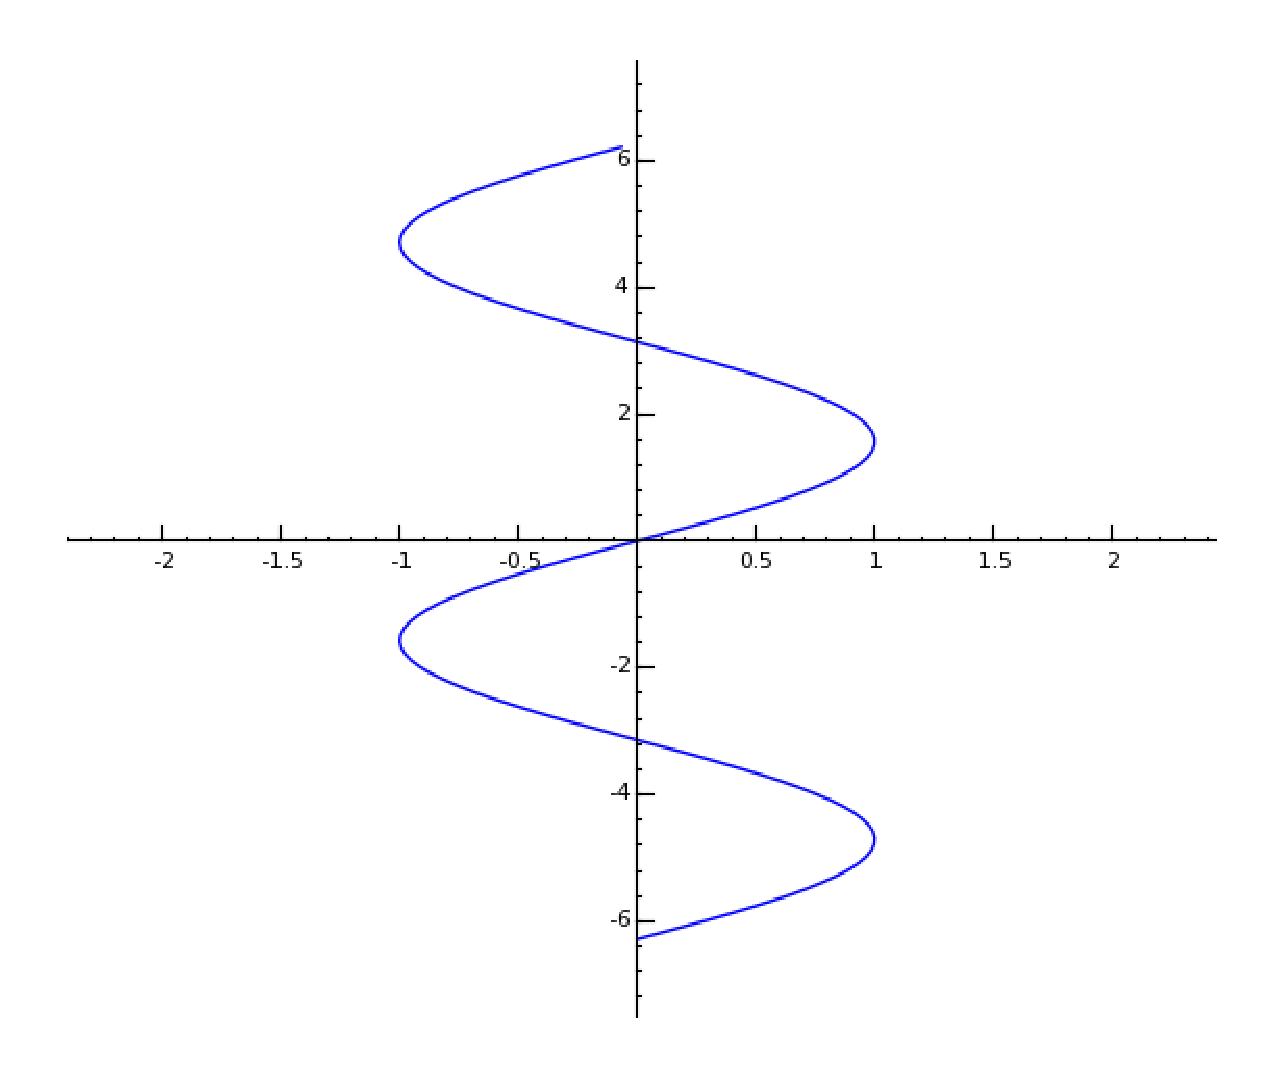
\includegraphics[height=6cm,width=7cm]{arcsin2.eps}%
\lthtmlpictureZ
\lthtmlcheckvsize\clearpage}

{\newpage\clearpage
\lthtmlinlinemathA{tex2html_wrap_inline47543}%
$ \sin^{-1}\  x$%
\lthtmlinlinemathZ
\lthtmlcheckvsize\clearpage}

{\newpage\clearpage
\lthtmlpictureA{tex2html_wrap47548}%
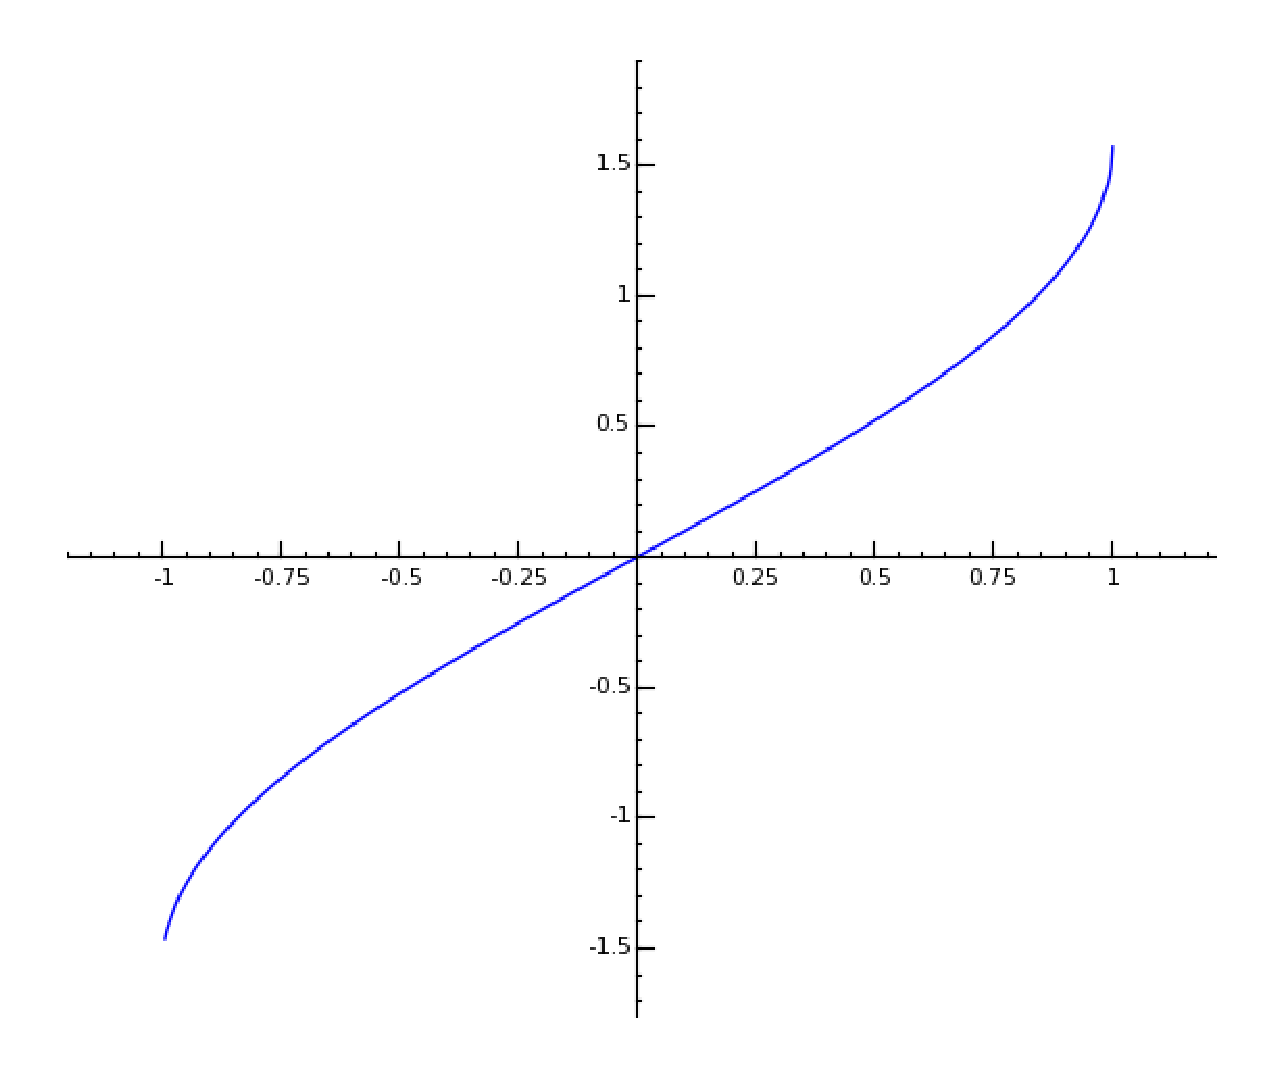
\includegraphics[height=3cm,width=3cm]{arcsin.eps}%
\lthtmlpictureZ
\lthtmlcheckvsize\clearpage}

{\newpage\clearpage
\lthtmlinlinemathA{tex2html_wrap_inline47552}%
$ f(x)=\arcsin(x)$%
\lthtmlinlinemathZ
\lthtmlcheckvsize\clearpage}

{\newpage\clearpage
\lthtmlinlinemathA{tex2html_wrap_inline47575}%
$ \frac{dv}{dy} 	= \cos\  y$%
\lthtmlinlinemathZ
\lthtmlcheckvsize\clearpage}

{\newpage\clearpage
\lthtmlinlinemathA{tex2html_wrap_inline47577}%
$ \frac{dy}{dv} = \frac{1}{\cos y}$%
\lthtmlinlinemathZ
\lthtmlcheckvsize\clearpage}

{\newpage\clearpage
\lthtmlinlinemathA{tex2html_wrap_indisplay47585}%
$\displaystyle \frac{dy}{dx} 	= \frac{1}{\cos y} \cdot \frac{dv}{dx} 	= \frac{1}{\sqrt{1 - v^2}} \frac{dv}{dx},
$%
\lthtmlindisplaymathZ
\lthtmlcheckvsize\clearpage}

{\newpage\clearpage
\lthtmlinlinemathA{tex2html_wrap_inline47587}%
$ \cos y = \sqrt{1 - \sin^2 y} = \sqrt{1 - v^2}$%
\lthtmlinlinemathZ
\lthtmlcheckvsize\clearpage}

{\newpage\clearpage
\lthtmlinlinemathA{tex2html_wrap_inline47589}%
$ \cos y$%
\lthtmlinlinemathZ
\lthtmlcheckvsize\clearpage}

{\newpage\clearpage
\lthtmlinlinemathA{tex2html_wrap_indisplay47597}%
$\displaystyle \frac{d}{dx}(\arcsin\, v) 	= \frac{\frac{dv}{dx}}{\sqrt{1 - v^2}}
$%
\lthtmlindisplaymathZ
\lthtmlcheckvsize\clearpage}

\stepcounter{section}
{\newpage\clearpage
\lthtmlinlinemathA{tex2html_wrap_inline47600}%
$ \arccos v$%
\lthtmlinlinemathZ
\lthtmlcheckvsize\clearpage}

{\newpage\clearpage
\lthtmlinlinemathA{tex2html_wrap_inline47619}%
$ y 	= \arccos\  v$%
\lthtmlinlinemathZ
\lthtmlcheckvsize\clearpage}

{\newpage\clearpage
\lthtmlinlinemathA{tex2html_wrap_inline47621}%
$ y 	= \cos\  y$%
\lthtmlinlinemathZ
\lthtmlcheckvsize\clearpage}

{\newpage\clearpage
\lthtmlpictureA{tex2html_wrap47623}%
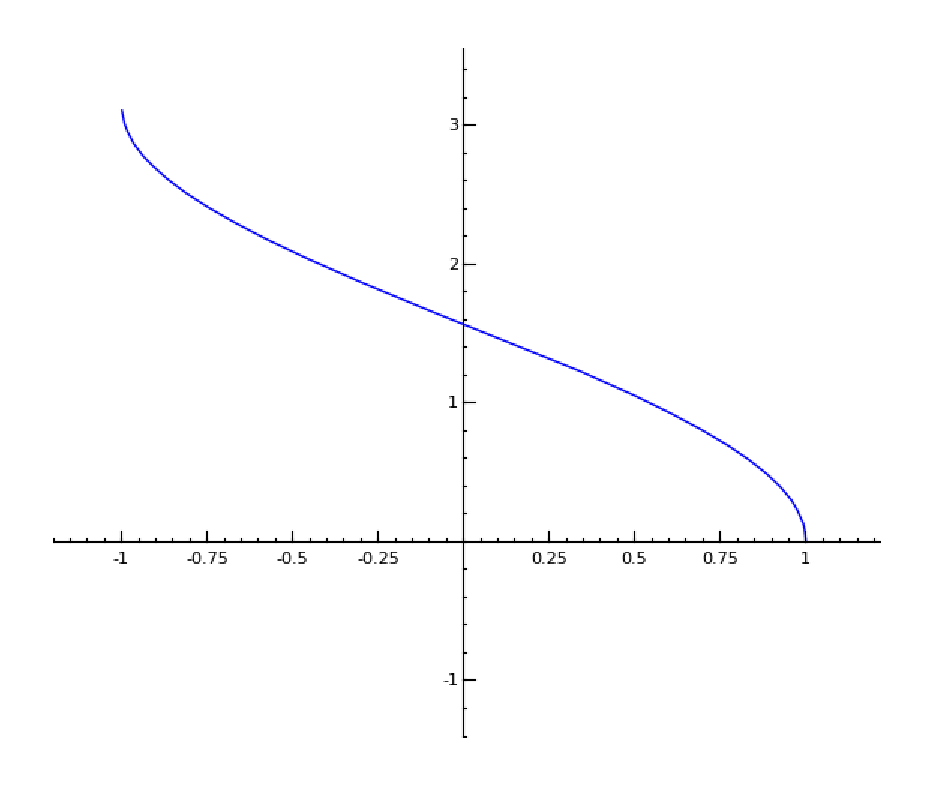
\includegraphics[height=3cm,width=3cm]{arccos2.eps}%
\lthtmlpictureZ
\lthtmlcheckvsize\clearpage}

{\newpage\clearpage
\lthtmlinlinemathA{tex2html_wrap_inline47627}%
$ f(x)=\arccos(x)$%
\lthtmlinlinemathZ
\lthtmlcheckvsize\clearpage}

{\newpage\clearpage
\lthtmlinlinemathA{tex2html_wrap_inline47634}%
$ \frac{dv}{dy} 	= -\sin\  y$%
\lthtmlinlinemathZ
\lthtmlcheckvsize\clearpage}

{\newpage\clearpage
\lthtmlinlinemathA{tex2html_wrap_inline47636}%
$ \frac{dy}{dv} = -\frac{1}{\sin y}$%
\lthtmlinlinemathZ
\lthtmlcheckvsize\clearpage}

{\newpage\clearpage
\lthtmlinlinemathA{tex2html_wrap_indisplay47644}%
$\displaystyle \frac{dy}{dx} 	= -\frac{1}{\sin y} \cdot \frac{dv}{dx}
= - \frac{1}{\sqrt{1 - v^2}} \frac{dv}{dx}
$%
\lthtmlindisplaymathZ
\lthtmlcheckvsize\clearpage}

{\newpage\clearpage
\lthtmlinlinemathA{tex2html_wrap_inline47646}%
$ \sin y = \sqrt{1 - \cos^2 y} = \sqrt{1 - v^2}$%
\lthtmlinlinemathZ
\lthtmlcheckvsize\clearpage}

{\newpage\clearpage
\lthtmlinlinemathA{tex2html_wrap_inline47648}%
$ \sin\, y$%
\lthtmlinlinemathZ
\lthtmlcheckvsize\clearpage}

{\newpage\clearpage
\lthtmlinlinemathA{tex2html_wrap_indisplay47655}%
$\displaystyle \frac{d}{dx}(\arccos\, v) 	= -\frac{\frac{dv}{dx}}{\sqrt{1 - v^2}}.
$%
\lthtmlindisplaymathZ
\lthtmlcheckvsize\clearpage}

{\newpage\clearpage
\lthtmlpictureA{tex2html_wrap47665}%
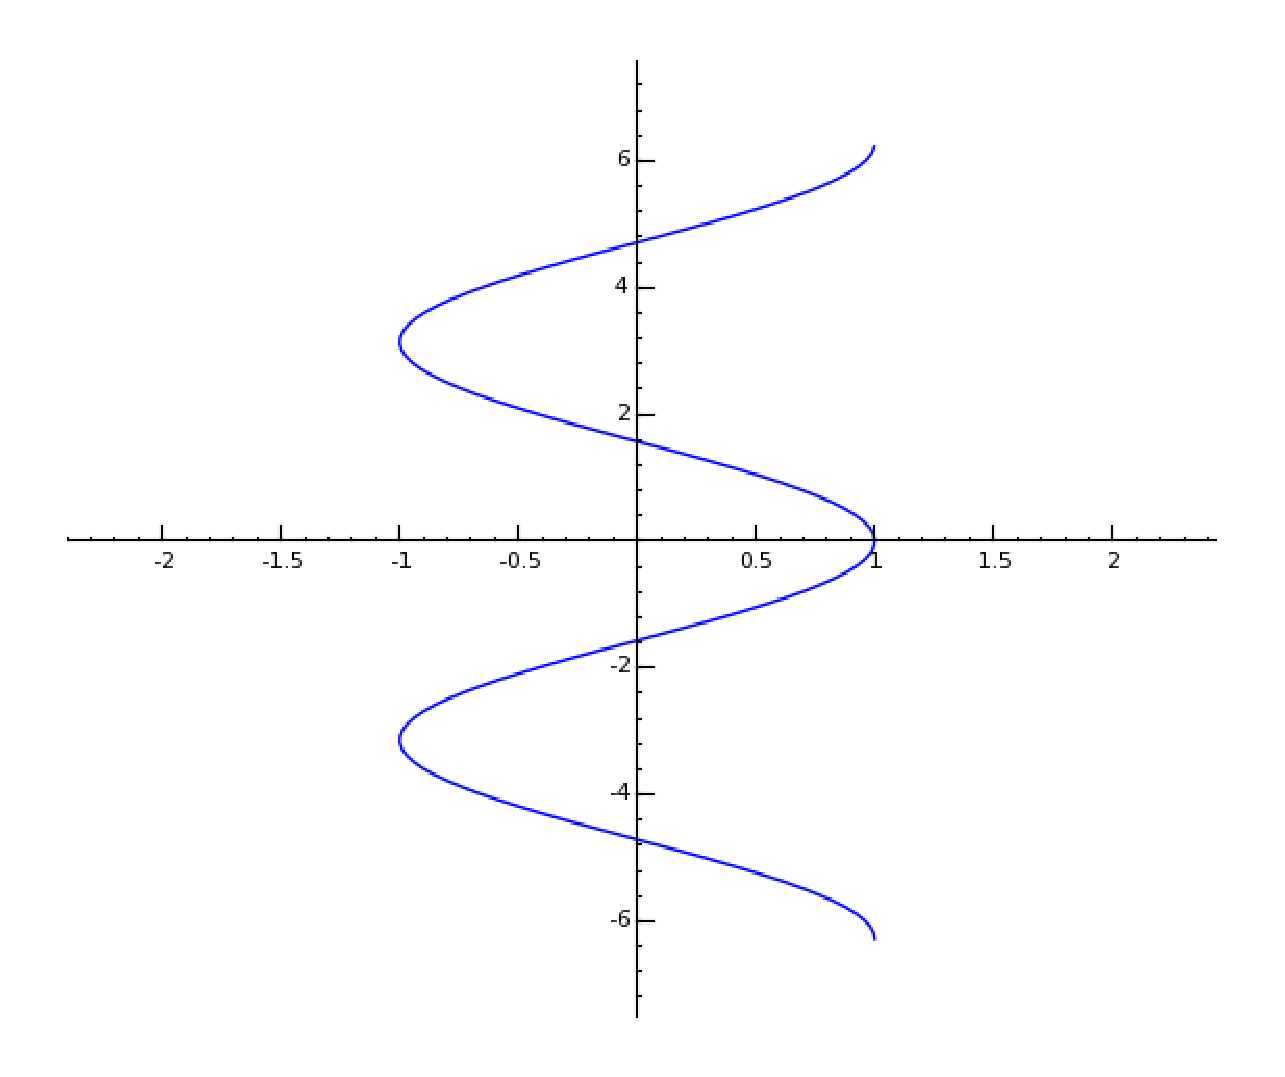
\includegraphics[height=6cm,width=7cm]{arccos.eps}%
\lthtmlpictureZ
\lthtmlcheckvsize\clearpage}

{\newpage\clearpage
\lthtmlinlinemathA{tex2html_wrap_inline47669}%
$ \cos^{-1}\  x$%
\lthtmlinlinemathZ
\lthtmlcheckvsize\clearpage}

\stepcounter{section}
{\newpage\clearpage
\lthtmlinlinemathA{tex2html_wrap_inline47675}%
$ \arctan\, v$%
\lthtmlinlinemathZ
\lthtmlcheckvsize\clearpage}

{\newpage\clearpage
\lthtmlinlinemathA{tex2html_wrap_inline47687}%
$ y 	=\  \arctan v$%
\lthtmlinlinemathZ
\lthtmlcheckvsize\clearpage}

{\newpage\clearpage
\lthtmlinlinemathA{tex2html_wrap_inline47689}%
$ y 	=\  \tan y$%
\lthtmlinlinemathZ
\lthtmlcheckvsize\clearpage}

{\newpage\clearpage
\lthtmlpictureA{tex2html_wrap47691}%
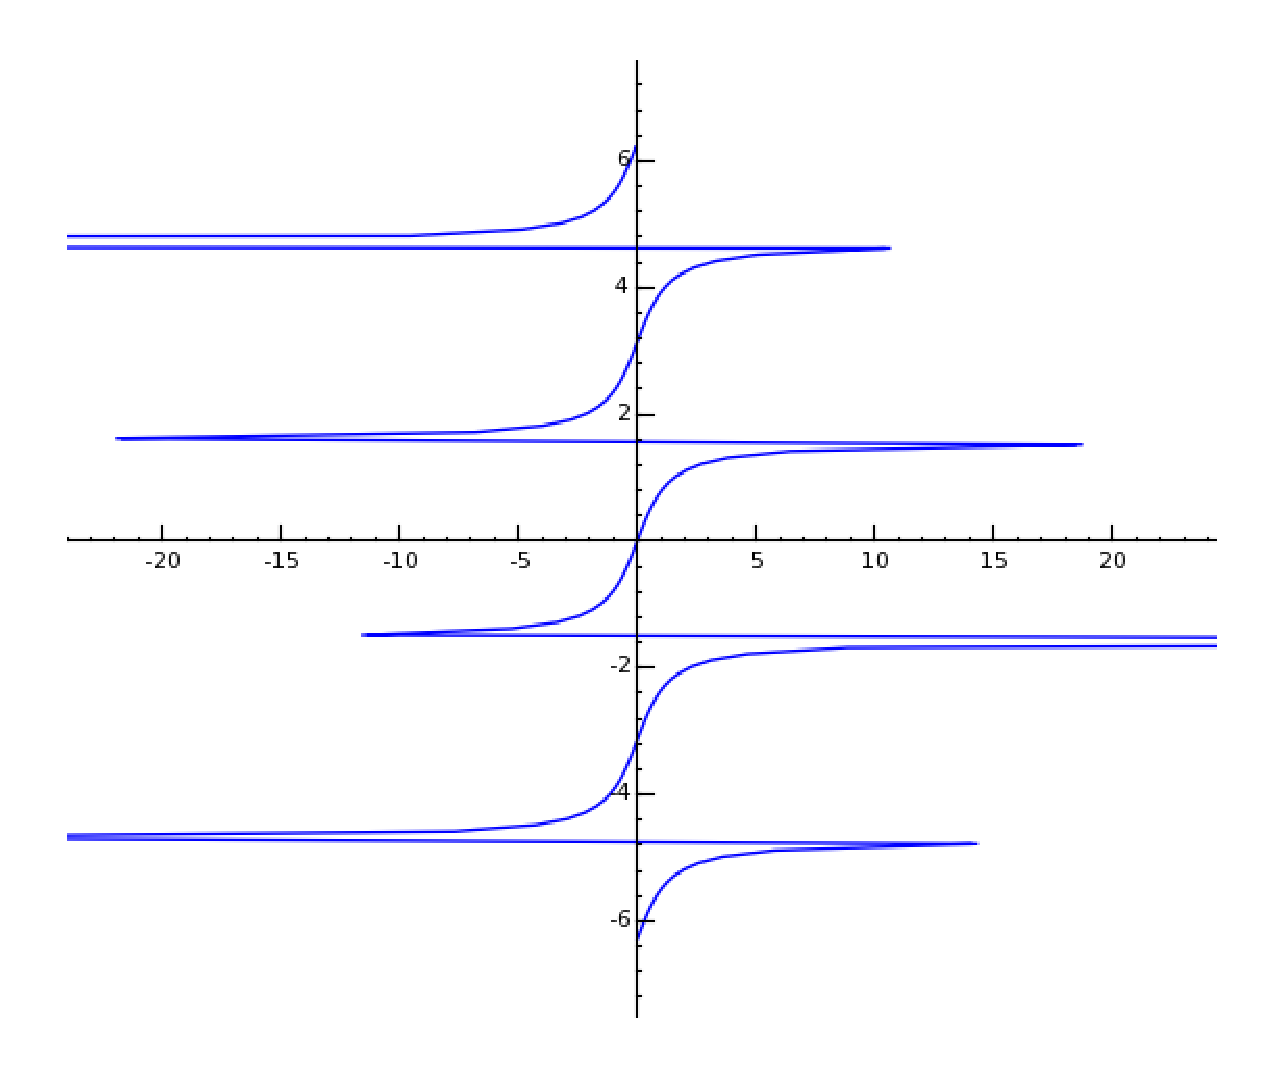
\includegraphics[height=6cm,width=7cm]{arctan2.eps}%
\lthtmlpictureZ
\lthtmlcheckvsize\clearpage}

{\newpage\clearpage
\lthtmlinlinemathA{tex2html_wrap_inline47695}%
$ \tan^{-1}\  x$%
\lthtmlinlinemathZ
\lthtmlcheckvsize\clearpage}

{\newpage\clearpage
\lthtmlpictureA{tex2html_wrap47700}%
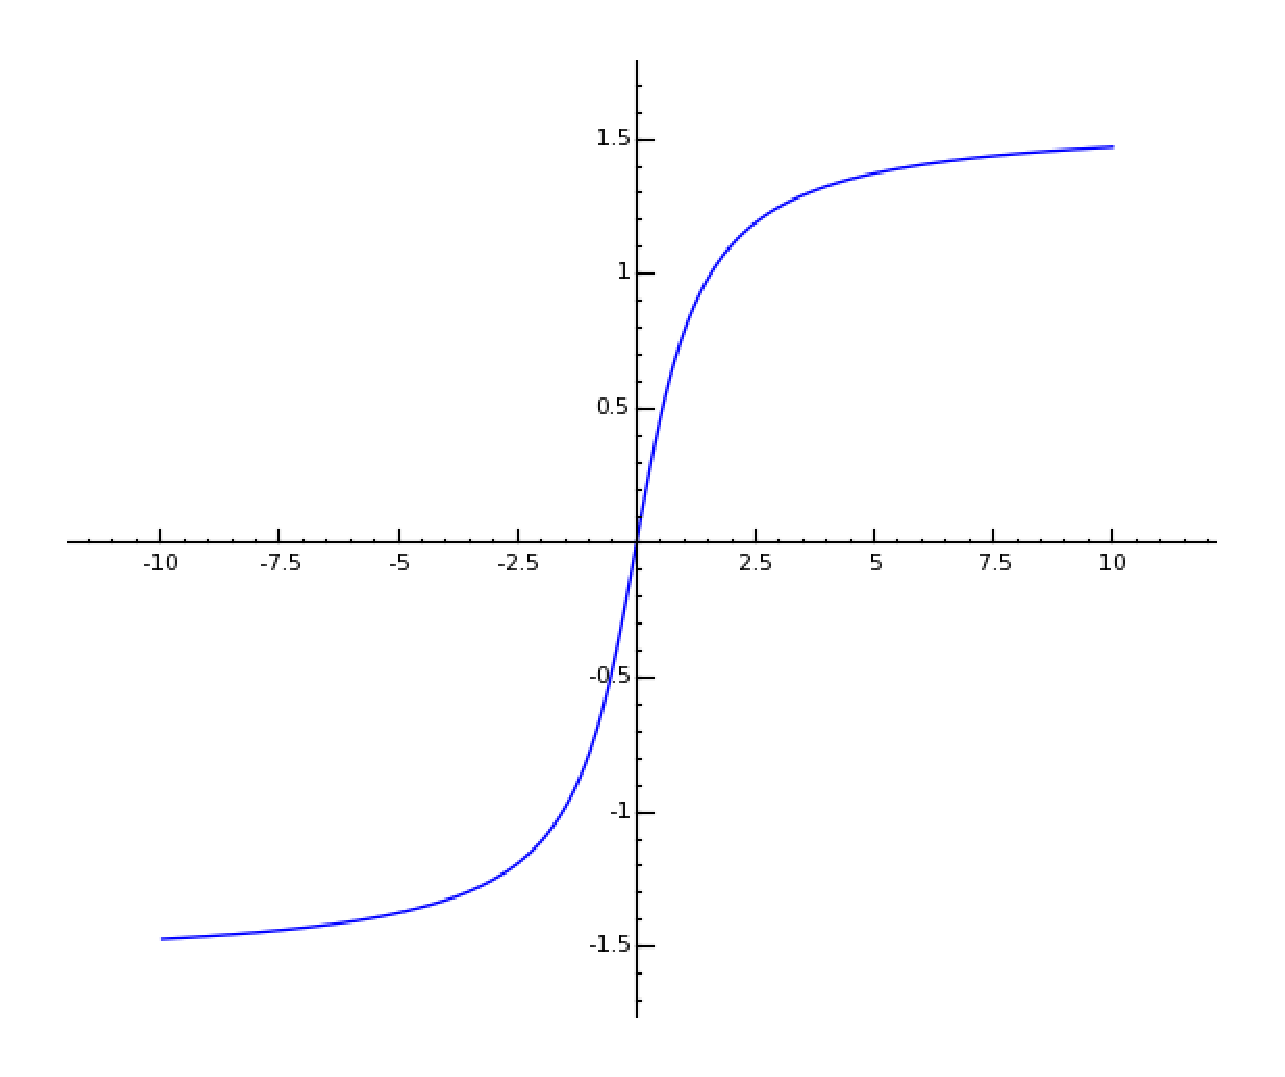
\includegraphics[height=5cm,width=8cm]{arctan.eps}%
\lthtmlpictureZ
\lthtmlcheckvsize\clearpage}

{\newpage\clearpage
\lthtmlinlinemathA{tex2html_wrap_indisplay47711}%
$\displaystyle \frac{dv}{dy} 	=\  \sec^2 y;
$%
\lthtmlindisplaymathZ
\lthtmlcheckvsize\clearpage}

{\newpage\clearpage
\lthtmlinlinemathA{tex2html_wrap_inline47713}%
$ \frac{dy}{dv} 	= \frac{1}{\sec^2 y}$%
\lthtmlinlinemathZ
\lthtmlcheckvsize\clearpage}

{\newpage\clearpage
\lthtmlinlinemathA{tex2html_wrap_indisplay47721}%
$\displaystyle \frac{dy}{dx} 	= \frac{1}{\sec^2 y} \cdot \frac{dv}{dx}
= \frac{1}{1 + v^2} \frac{dv}{dx},
$%
\lthtmlindisplaymathZ
\lthtmlcheckvsize\clearpage}

{\newpage\clearpage
\lthtmlinlinemathA{tex2html_wrap_inline47723}%
$ \sec^2y = 1 + \tan^2y = 1 + v^2$%
\lthtmlinlinemathZ
\lthtmlcheckvsize\clearpage}

{\newpage\clearpage
\lthtmlinlinemathA{tex2html_wrap_indisplay47725}%
$\displaystyle \frac{d}{dx} (\arctan\, v) 	= \frac{\frac{dv}{dx}}{1 + v^2}
$%
\lthtmlindisplaymathZ
\lthtmlcheckvsize\clearpage}

\stepcounter{section}
{\newpage\clearpage
\lthtmlinlinemathA{tex2html_wrap_inline47730}%
$ y 	= {\rm arccot}\  v$%
\lthtmlinlinemathZ
\lthtmlcheckvsize\clearpage}

{\newpage\clearpage
\lthtmlinlinemathA{tex2html_wrap_inline47732}%
$ y 	= \cot\  y$%
\lthtmlinlinemathZ
\lthtmlcheckvsize\clearpage}

{\newpage\clearpage
\lthtmlinlinemathA{tex2html_wrap_indisplay47743}%
$\displaystyle \frac{d}{dx}({\rm arccot}\, v) = -\frac{\frac{dv}{dx}}{1 + v^2}
$%
\lthtmlindisplaymathZ
\lthtmlcheckvsize\clearpage}

\stepcounter{section}
{\newpage\clearpage
\lthtmlinlinemathA{tex2html_wrap_inline47748}%
$ y 	=\  {\rm arcsec}v$%
\lthtmlinlinemathZ
\lthtmlcheckvsize\clearpage}

{\newpage\clearpage
\lthtmlinlinemathA{tex2html_wrap_inline47750}%
$ v 	=\  \sec y$%
\lthtmlinlinemathZ
\lthtmlcheckvsize\clearpage}

{\newpage\clearpage
\lthtmlinlinemathA{tex2html_wrap_inline47774}%
$ DC$%
\lthtmlinlinemathZ
\lthtmlcheckvsize\clearpage}

{\newpage\clearpage
\lthtmlinlinemathA{tex2html_wrap_inline47778}%
$ -\pi$%
\lthtmlinlinemathZ
\lthtmlcheckvsize\clearpage}

{\newpage\clearpage
\lthtmlpictureA{tex2html_wrap47784}%
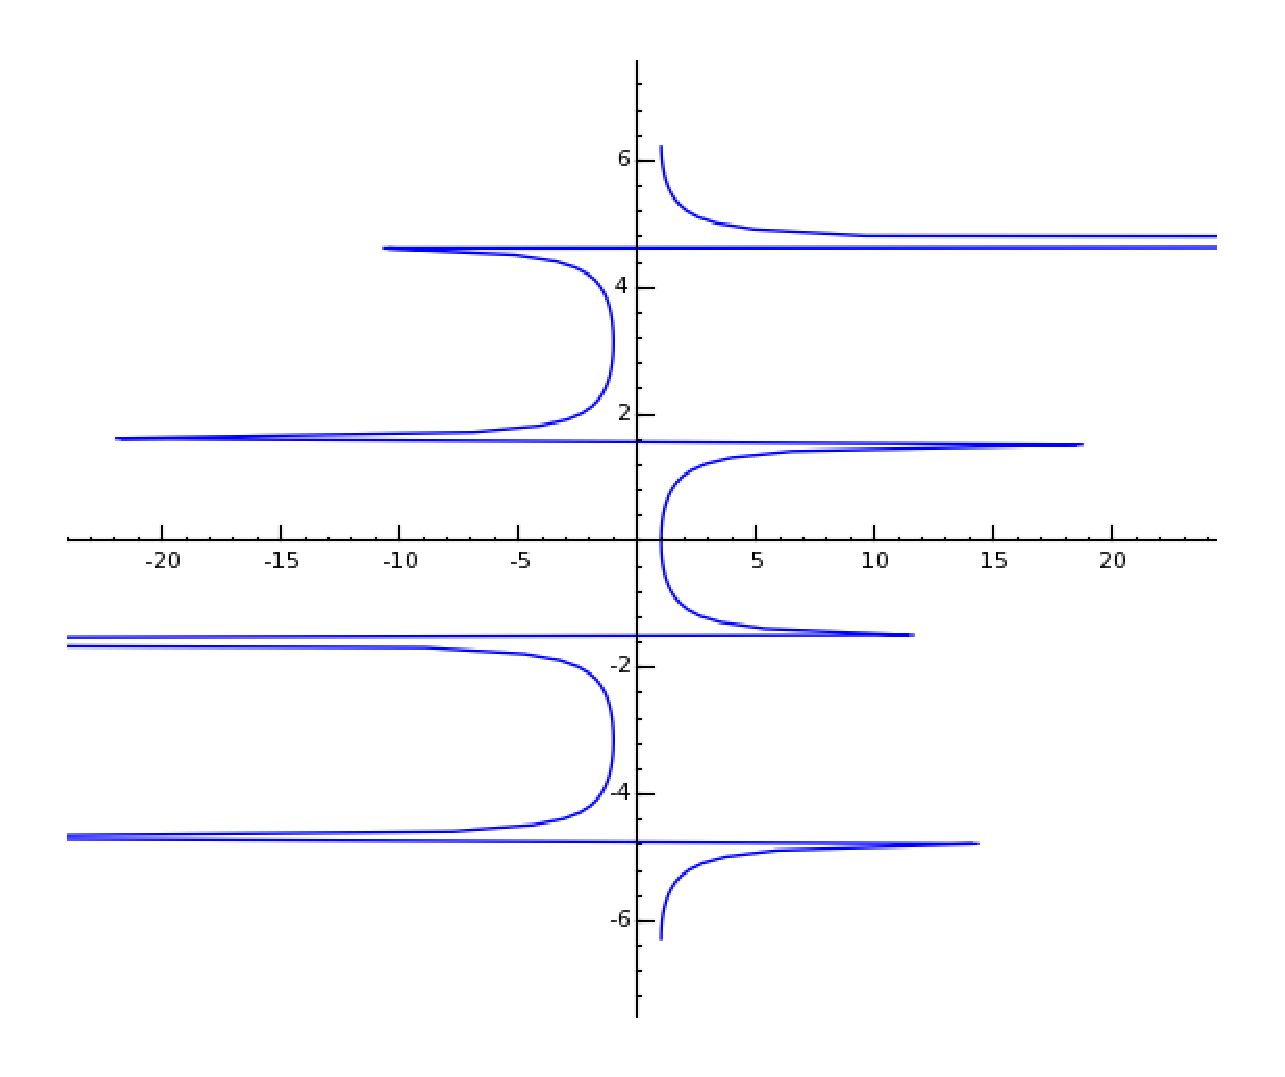
\includegraphics[height=6cm,width=7cm]{arcsec3.eps}%
\lthtmlpictureZ
\lthtmlcheckvsize\clearpage}

{\newpage\clearpage
\lthtmlinlinemathA{tex2html_wrap_inline47788}%
$ \sec^{-1}\  x$%
\lthtmlinlinemathZ
\lthtmlcheckvsize\clearpage}

{\newpage\clearpage
\lthtmlpictureA{tex2html_wrap47793}%
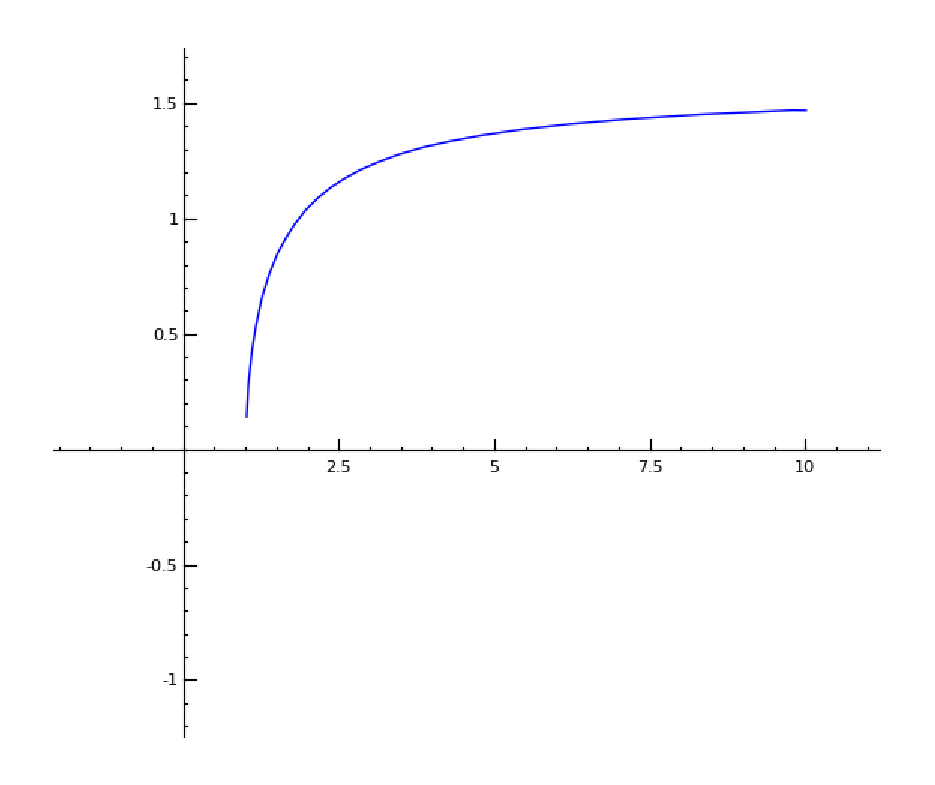
\includegraphics[height=5cm,width=8cm]{arcsec2.eps}%
\lthtmlpictureZ
\lthtmlcheckvsize\clearpage}

{\newpage\clearpage
\lthtmlinlinemathA{tex2html_wrap_inline47804}%
$ \frac{dv}{dy} 	=\  \sec y \tan y$%
\lthtmlinlinemathZ
\lthtmlcheckvsize\clearpage}

{\newpage\clearpage
\lthtmlinlinemathA{tex2html_wrap_inline47806}%
$ \frac{dy}{dv} 	= \frac{1}{\sec y \tan y}$%
\lthtmlinlinemathZ
\lthtmlcheckvsize\clearpage}

{\newpage\clearpage
\lthtmlinlinemathA{tex2html_wrap_indisplay47814}%
$\displaystyle \frac{dy}{dx} 	= \frac{1}{\sec y \tan y} \frac{dv}{dx}
= \frac{1}{v \sqrt{v^2 - 1}} \frac{dv}{dx}
$%
\lthtmlindisplaymathZ
\lthtmlcheckvsize\clearpage}

{\newpage\clearpage
\lthtmlinlinemathA{tex2html_wrap_inline47816}%
$ \sec y = v$%
\lthtmlinlinemathZ
\lthtmlcheckvsize\clearpage}

{\newpage\clearpage
\lthtmlinlinemathA{tex2html_wrap_inline47818}%
$ \tan y = \sqrt{\sec y - 1} = \sqrt{v^2 - 1}$%
\lthtmlinlinemathZ
\lthtmlcheckvsize\clearpage}

{\newpage\clearpage
\lthtmlinlinemathA{tex2html_wrap_inline47820}%
$ \tan y$%
\lthtmlinlinemathZ
\lthtmlcheckvsize\clearpage}

{\newpage\clearpage
\lthtmlinlinemathA{tex2html_wrap_indisplay47834}%
$\displaystyle \frac{d}{dx} ({\rm arcsec}v) 	= \frac{\frac{dv}{dx}}{v \sqrt{v^2 - 1}}
$%
\lthtmlindisplaymathZ
\lthtmlcheckvsize\clearpage}

\stepcounter{section}
{\newpage\clearpage
\lthtmlinlinemathA{tex2html_wrap_inline47837}%
$ {\rm arccsc}\, v$%
\lthtmlinlinemathZ
\lthtmlcheckvsize\clearpage}

{\newpage\clearpage
\lthtmlinlinemathA{tex2html_wrap_indisplay47839}%
$\displaystyle y 	=\  {\rm arccsc}\, v; 
$%
\lthtmlindisplaymathZ
\lthtmlcheckvsize\clearpage}

{\newpage\clearpage
\lthtmlinlinemathA{tex2html_wrap_indisplay47841}%
$\displaystyle v =\  \csc\, y.
$%
\lthtmlindisplaymathZ
\lthtmlcheckvsize\clearpage}

{\newpage\clearpage
\lthtmlinlinemathA{tex2html_wrap_inline47866}%
$ CD$%
\lthtmlinlinemathZ
\lthtmlcheckvsize\clearpage}

{\newpage\clearpage
\lthtmlpictureA{tex2html_wrap47876}%
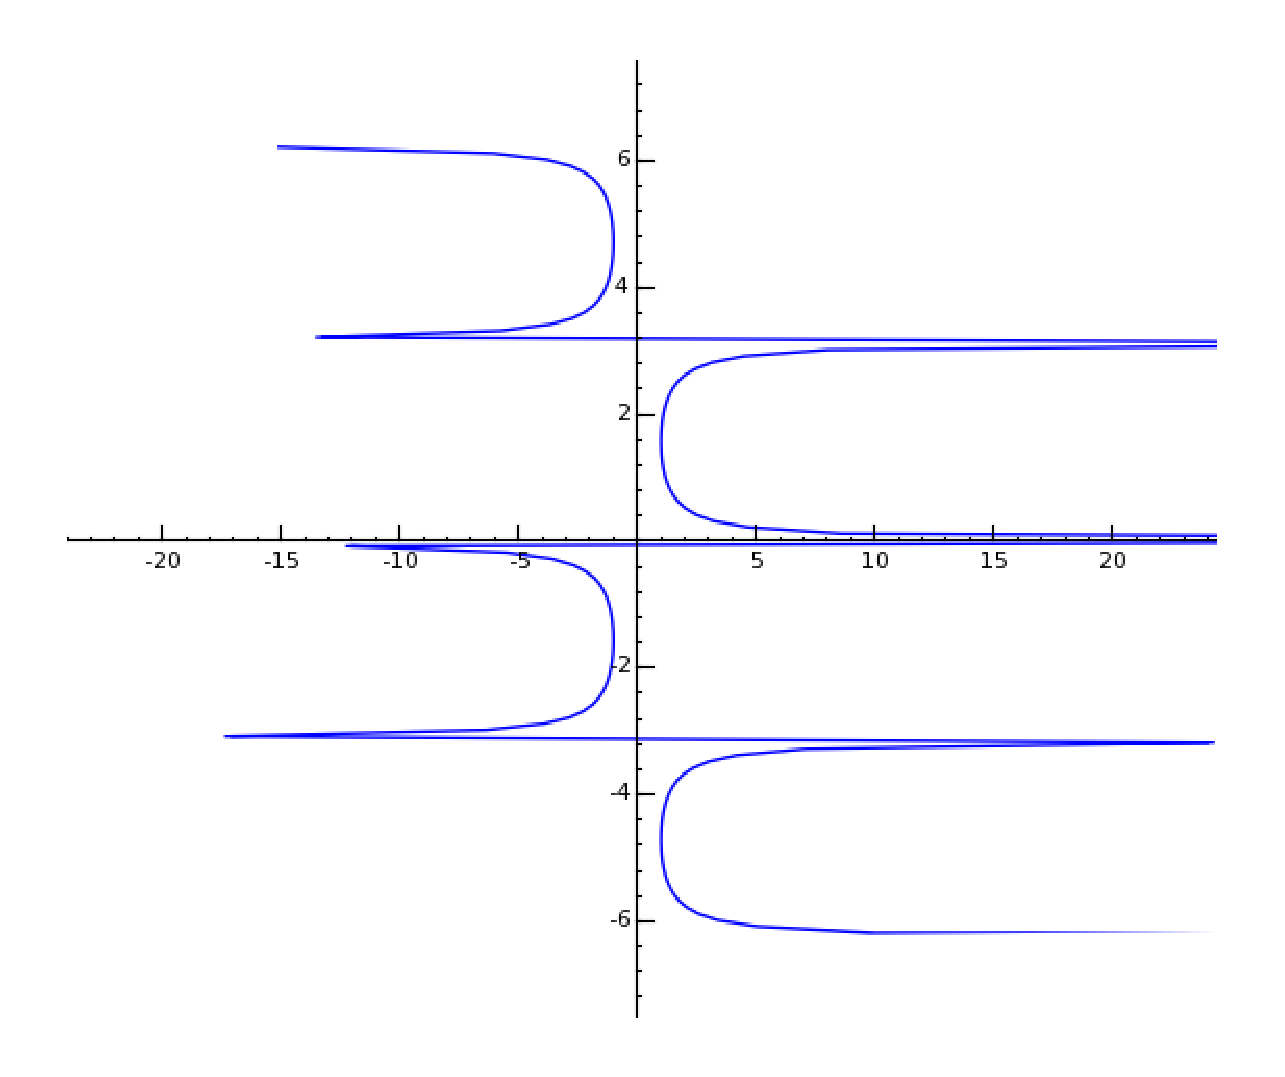
\includegraphics[height=6cm,width=7cm]{arccsc2.eps}%
\lthtmlpictureZ
\lthtmlcheckvsize\clearpage}

{\newpage\clearpage
\lthtmlpictureA{tex2html_wrap47885}%
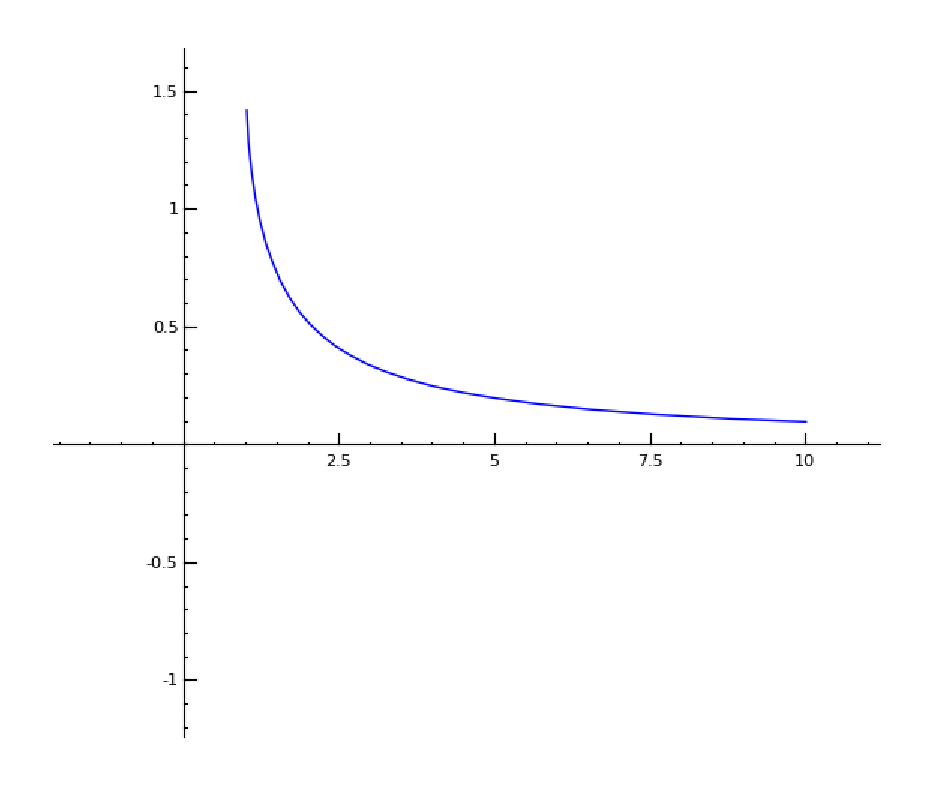
\includegraphics[height=5cm,width=8cm]{arccsc3.eps}%
\lthtmlpictureZ
\lthtmlcheckvsize\clearpage}

{\newpage\clearpage
\lthtmlinlinemathA{tex2html_wrap_indisplay47896}%
$\displaystyle \frac{d}{dx}({\rm arccsc}v) 	= -\frac{\frac{dv}{dx}}{v\sqrt{v^2 - 1}}
$%
\lthtmlindisplaymathZ
\lthtmlcheckvsize\clearpage}

\stepcounter{section}
{\newpage\clearpage
\lthtmlinlinemathA{tex2html_wrap_inline47899}%
$ {\rm arcvers}\, v$%
\lthtmlinlinemathZ
\lthtmlcheckvsize\clearpage}

{\newpage\clearpage
\lthtmlinlinemathA{tex2html_wrap_inline47917}%
$ y 	= {\rm arcvers}\, v$%
\lthtmlinlinemathZ
\lthtmlcheckvsize\clearpage}

{\newpage\clearpage
\lthtmlinlinemathA{tex2html_wrap_inline47919}%
$ v = {\rm vers}\, y$%
\lthtmlinlinemathZ
\lthtmlcheckvsize\clearpage}

{\newpage\clearpage
\lthtmlinlinemathA{tex2html_wrap_indisplay47923}%
$\displaystyle \frac{dv}{dy} 	=\  \sin y;
$%
\lthtmlindisplaymathZ
\lthtmlcheckvsize\clearpage}

{\newpage\clearpage
\lthtmlinlinemathA{tex2html_wrap_inline47925}%
$ \frac{dy}{dv} 	= \frac{1}{\sin y}$%
\lthtmlinlinemathZ
\lthtmlcheckvsize\clearpage}

{\newpage\clearpage
\lthtmlinlinemathA{tex2html_wrap_indisplay47933}%
$\displaystyle \frac{dy}{dx} 	= \frac{1}{\sin y} \cdot \frac{dv}{dx}
= \frac{1}{\sqrt{2v - v^2}} \frac{dv}{dx}
$%
\lthtmlindisplaymathZ
\lthtmlcheckvsize\clearpage}

{\newpage\clearpage
\lthtmlinlinemathA{tex2html_wrap_inline47935}%
$ \sin y = \sqrt{1 - \cos^2 y} = \sqrt{1 - (1 - {\rm vers}\, y)^2} 
= \sqrt{2v - v^2}$%
\lthtmlinlinemathZ
\lthtmlcheckvsize\clearpage}

{\newpage\clearpage
\lthtmlinlinemathA{tex2html_wrap_indisplay47944}%
$\displaystyle \frac{d}{dx} (\operatorname{arcvers}\, v) 	= \frac{\frac{dv}{dx}}{\sqrt{2v - v^2}}
$%
\lthtmlindisplaymathZ
\lthtmlcheckvsize\clearpage}

\stepcounter{section}
{\newpage\clearpage
\lthtmlinlinemathA{tex2html_wrap_inline47947}%
$ y = \arctan (ax^2)$%
\lthtmlinlinemathZ
\lthtmlcheckvsize\clearpage}

{\newpage\clearpage
\lthtmlinlinemathA{tex2html_wrap_inline47949}%
$ v = ax^2$%
\lthtmlinlinemathZ
\lthtmlcheckvsize\clearpage}

{\newpage\clearpage
\lthtmlinlinemathA{tex2html_wrap_indisplay47951}%
$\displaystyle \frac{dy}{dx} 	= \frac{\frac{d}{dx} (ax^2)}{1 + (ax^2)^2} 
= \frac{2ax}{1 + a^2x^4}.
$%
\lthtmlindisplaymathZ
\lthtmlcheckvsize\clearpage}

{\newpage\clearpage
\lthtmlinlinemathA{tex2html_wrap_inline47953}%
$ y = \arcsin(3x - 4x^3)$%
\lthtmlinlinemathZ
\lthtmlcheckvsize\clearpage}

{\newpage\clearpage
\lthtmlinlinemathA{tex2html_wrap_inline47955}%
$ v = 3x - 4x^3$%
\lthtmlinlinemathZ
\lthtmlcheckvsize\clearpage}

{\newpage\clearpage
\lthtmlinlinemathA{tex2html_wrap_indisplay47957}%
$\displaystyle \frac{dy}{dx} =	\frac{\frac{d}{dx}(3x - 4x^3)}{\sqrt{1 - (3x - 4x^3)^2}}
=\frac{3 - 12x^2}{\sqrt{1 - 9x^2 + 24x^4 - 16x^6}} = \frac{3}{\sqrt{1 - x^2}}.
$%
\lthtmlindisplaymathZ
\lthtmlcheckvsize\clearpage}

{\newpage\clearpage
\lthtmlinlinemathA{tex2html_wrap_inline47959}%
$ y={\rm arcsec}\, \frac{x^2 + 1}{x^2 - 1}$%
\lthtmlinlinemathZ
\lthtmlcheckvsize\clearpage}

{\newpage\clearpage
\lthtmlinlinemathA{tex2html_wrap_inline47961}%
$ v =  \frac{x^2 + 1}{x^2 - 1} $%
\lthtmlinlinemathZ
\lthtmlcheckvsize\clearpage}

{\newpage\clearpage
\lthtmlinlinemathA{tex2html_wrap_indisplay47963}%
$\displaystyle \frac{dy}{dx} 	
= \frac{\frac{d}{dx} \left ( \frac{x^2 + 1}{x^2 - 1} \right )}{\frac{x^2 + 1}{x^2 - 1} \sqrt{\left ( \frac{x^2 + 1}{x^2 - 1} \right )^2 - 1}} 	
= \frac{\frac{(x^2 - 1)2x - (x^2 + 1)2x}{(x^2 - 1)^2}}{\frac{x^2 + 1}{x^2 - 1} \cdot \frac{2x}{x^2 - 1}} 
= -\frac{2}{x^2 + 1}.
$%
\lthtmlindisplaymathZ
\lthtmlcheckvsize\clearpage}

{\newpage\clearpage
\lthtmlinlinemathA{tex2html_wrap_inline47965}%
$ \frac{d}{dx} \arcsin \frac{x}{a} = \frac{1}{\sqrt{a^2 - x^2}}$%
\lthtmlinlinemathZ
\lthtmlcheckvsize\clearpage}

{\newpage\clearpage
\lthtmlinlinemathA{tex2html_wrap_inline47967}%
$ \frac{d}{dx} {\rm arccot}(x^2 - 5) = \frac{-2x}{1 + (x^2 - 5)^2}$%
\lthtmlinlinemathZ
\lthtmlcheckvsize\clearpage}

{\newpage\clearpage
\lthtmlinlinemathA{tex2html_wrap_inline47969}%
$ \frac{d}{dx} \arctan \frac{2x}{1 - x^2} = \frac{2}{1 + x^2}$%
\lthtmlinlinemathZ
\lthtmlcheckvsize\clearpage}

{\newpage\clearpage
\lthtmlinlinemathA{tex2html_wrap_inline47971}%
$ \frac{d}{dx} {\rm arccsc}\frac{1}{2x^2 - 1} = \frac{2}{\sqrt{1 - x^2}}$%
\lthtmlinlinemathZ
\lthtmlcheckvsize\clearpage}

{\newpage\clearpage
\lthtmlinlinemathA{tex2html_wrap_inline47973}%
$ \frac{d}{dx} \operatorname{arcvers}\, 2x^2 = \frac{2}{\sqrt{1 - x^2}}$%
\lthtmlinlinemathZ
\lthtmlcheckvsize\clearpage}

{\newpage\clearpage
\lthtmlinlinemathA{tex2html_wrap_inline47975}%
$ \frac{d}{dx} \arctan \sqrt{1 - x} = -\frac{1}{2 \sqrt{1 - x} (2 - x)}$%
\lthtmlinlinemathZ
\lthtmlcheckvsize\clearpage}

{\newpage\clearpage
\lthtmlinlinemathA{tex2html_wrap_inline47977}%
$ \frac{d}{dx} {\rm arccsc}\frac{3}{2x} = \frac{2}{9 - 4x^2}$%
\lthtmlinlinemathZ
\lthtmlcheckvsize\clearpage}

{\newpage\clearpage
\lthtmlinlinemathA{tex2html_wrap_inline47979}%
$ \frac{d}{dx} \operatorname{arcvers}\, \frac{2x^2}{1 + x^2} = \frac{2}{1 + x^2}$%
\lthtmlinlinemathZ
\lthtmlcheckvsize\clearpage}

{\newpage\clearpage
\lthtmlinlinemathA{tex2html_wrap_inline47981}%
$ \frac{d}{dx} \arctan \frac{x}{a} = \frac{a}{a^2 + x^2}$%
\lthtmlinlinemathZ
\lthtmlcheckvsize\clearpage}

{\newpage\clearpage
\lthtmlinlinemathA{tex2html_wrap_inline47983}%
$ \frac{d}{dx} \arcsin \frac{x + 1}{\sqrt{2}} = \frac{1}{\sqrt{1 - 2x - x^2}}$%
\lthtmlinlinemathZ
\lthtmlcheckvsize\clearpage}

{\newpage\clearpage
\lthtmlinlinemathA{tex2html_wrap_inline47985}%
$ f(x) = x\sqrt{a^2 - x^2} + a^2 \arcsin \frac{x}{a}$%
\lthtmlinlinemathZ
\lthtmlcheckvsize\clearpage}

{\newpage\clearpage
\lthtmlinlinemathA{tex2html_wrap_inline47987}%
$ f'(x) =\  2\sqrt{a^2 - x^2}$%
\lthtmlinlinemathZ
\lthtmlcheckvsize\clearpage}

{\newpage\clearpage
\lthtmlinlinemathA{tex2html_wrap_inline47989}%
$ f(x) = \sqrt{a^2 - x^2} + a \arcsin \frac{x}{a}$%
\lthtmlinlinemathZ
\lthtmlcheckvsize\clearpage}

{\newpage\clearpage
\lthtmlinlinemathA{tex2html_wrap_inline47991}%
$ f'(x) 	= \left ( \frac{a - x}{a + x} \right )^{\frac{1}{2}}$%
\lthtmlinlinemathZ
\lthtmlcheckvsize\clearpage}

{\newpage\clearpage
\lthtmlinlinemathA{tex2html_wrap_inline47993}%
$ x = r {\rm arcvers}\, \frac{y}{r} - \sqrt{2ry - y^2}$%
\lthtmlinlinemathZ
\lthtmlcheckvsize\clearpage}

{\newpage\clearpage
\lthtmlinlinemathA{tex2html_wrap_inline47995}%
$ \frac{dx}{dy} 	= \frac{y}{\sqrt{2ry - y^2}}$%
\lthtmlinlinemathZ
\lthtmlcheckvsize\clearpage}

{\newpage\clearpage
\lthtmlinlinemathA{tex2html_wrap_inline47997}%
$ \theta = \arcsin (3r - 1)$%
\lthtmlinlinemathZ
\lthtmlcheckvsize\clearpage}

{\newpage\clearpage
\lthtmlinlinemathA{tex2html_wrap_inline47999}%
$ \frac{d\theta}{dr} 	= \frac{3}{\sqrt{6r - 9r^2}}$%
\lthtmlinlinemathZ
\lthtmlcheckvsize\clearpage}

{\newpage\clearpage
\lthtmlinlinemathA{tex2html_wrap_inline48001}%
$ \phi = \arctan \frac{r + a}{1 - ar}$%
\lthtmlinlinemathZ
\lthtmlcheckvsize\clearpage}

{\newpage\clearpage
\lthtmlinlinemathA{tex2html_wrap_inline48003}%
$ \frac{d\phi}{dr} 	= \frac{1}{1 + r^2}$%
\lthtmlinlinemathZ
\lthtmlcheckvsize\clearpage}

{\newpage\clearpage
\lthtmlinlinemathA{tex2html_wrap_inline48005}%
$ s = {\rm arcsec}\frac{1}{\sqrt{1 - t^2}}$%
\lthtmlinlinemathZ
\lthtmlcheckvsize\clearpage}

{\newpage\clearpage
\lthtmlinlinemathA{tex2html_wrap_inline48007}%
$ \frac{ds}{dt} =	\frac{1}{\sqrt{1 - t^2}}$%
\lthtmlinlinemathZ
\lthtmlcheckvsize\clearpage}

{\newpage\clearpage
\lthtmlinlinemathA{tex2html_wrap_inline48009}%
$ \frac{d}{dx} ( x \arcsin\, x) = \arcsin\, x + \frac{x}{\sqrt{1 - x^2}}$%
\lthtmlinlinemathZ
\lthtmlcheckvsize\clearpage}

{\newpage\clearpage
\lthtmlinlinemathA{tex2html_wrap_inline48011}%
$ \frac{d}{d\theta} (\tan \theta \arctan\, \theta) 
= \sec^2 \theta \arctan\, \theta \frac{\tan \theta}{1 + \theta^2}$%
\lthtmlinlinemathZ
\lthtmlcheckvsize\clearpage}

{\newpage\clearpage
\lthtmlinlinemathA{tex2html_wrap_inline48013}%
$ \frac{d}{dt}[\log (\arccos\, t)] = -\frac{1}{\arccos t \sqrt{1 - t^2}}$%
\lthtmlinlinemathZ
\lthtmlcheckvsize\clearpage}

{\newpage\clearpage
\lthtmlinlinemathA{tex2html_wrap_inline48015}%
$ f(y) = \arccos (\log\, y)$%
\lthtmlinlinemathZ
\lthtmlcheckvsize\clearpage}

{\newpage\clearpage
\lthtmlinlinemathA{tex2html_wrap_inline48017}%
$ f'(y) 	= -\frac{1}{y\sqrt{1 - (\log y)^2}}$%
\lthtmlinlinemathZ
\lthtmlcheckvsize\clearpage}

{\newpage\clearpage
\lthtmlinlinemathA{tex2html_wrap_inline48019}%
$ f(\theta) = \arcsin \sqrt{\sin \theta}$%
\lthtmlinlinemathZ
\lthtmlcheckvsize\clearpage}

{\newpage\clearpage
\lthtmlinlinemathA{tex2html_wrap_inline48021}%
$ f'(\theta) 	= \frac{1}{2} \sqrt{1 + \csc \theta}$%
\lthtmlinlinemathZ
\lthtmlcheckvsize\clearpage}

{\newpage\clearpage
\lthtmlinlinemathA{tex2html_wrap_inline48023}%
$ f(\phi) = \arctan \sqrt{\frac{1 - \cos \phi}{1 + \cos \phi}}$%
\lthtmlinlinemathZ
\lthtmlcheckvsize\clearpage}

{\newpage\clearpage
\lthtmlinlinemathA{tex2html_wrap_inline48025}%
$ f'(\phi) 	= \frac{1}{2}$%
\lthtmlinlinemathZ
\lthtmlcheckvsize\clearpage}

{\newpage\clearpage
\lthtmlinlinemathA{tex2html_wrap_inline48027}%
$ p = e^{\arctan\, q}$%
\lthtmlinlinemathZ
\lthtmlcheckvsize\clearpage}

{\newpage\clearpage
\lthtmlinlinemathA{tex2html_wrap_inline48029}%
$ \frac{dp}{dq} 	= \frac{e^{\arctan\, q}}{1 + q^2}$%
\lthtmlinlinemathZ
\lthtmlcheckvsize\clearpage}

{\newpage\clearpage
\lthtmlinlinemathA{tex2html_wrap_inline48031}%
$ u = \arctan \frac{e^v - e^{-v}}{2}$%
\lthtmlinlinemathZ
\lthtmlcheckvsize\clearpage}

{\newpage\clearpage
\lthtmlinlinemathA{tex2html_wrap_inline48033}%
$ \frac{du}{dv} 	= \frac{2}{e^v + e^{-v}}$%
\lthtmlinlinemathZ
\lthtmlcheckvsize\clearpage}

{\newpage\clearpage
\lthtmlinlinemathA{tex2html_wrap_inline48035}%
$ s = \arccos \frac{e^t - e^{-t}}{e^t + e^{-t}}$%
\lthtmlinlinemathZ
\lthtmlcheckvsize\clearpage}

{\newpage\clearpage
\lthtmlinlinemathA{tex2html_wrap_inline48037}%
$ \frac{ds}{dt} 	= -\frac{2}{e^v + e^{-v}}$%
\lthtmlinlinemathZ
\lthtmlcheckvsize\clearpage}

{\newpage\clearpage
\lthtmlinlinemathA{tex2html_wrap_inline48039}%
$ y = x^{\arcsin x}$%
\lthtmlinlinemathZ
\lthtmlcheckvsize\clearpage}

{\newpage\clearpage
\lthtmlinlinemathA{tex2html_wrap_inline48041}%
$ y' = x^{\arcsin x} \left ( \frac{\arcsin x}{x} + \frac{\log x}{\sqrt{1 - x^2}} \right )$%
\lthtmlinlinemathZ
\lthtmlcheckvsize\clearpage}

{\newpage\clearpage
\lthtmlinlinemathA{tex2html_wrap_inline48043}%
$ y = e^{x^x} \arctan\, x$%
\lthtmlinlinemathZ
\lthtmlcheckvsize\clearpage}

{\newpage\clearpage
\lthtmlinlinemathA{tex2html_wrap_inline48045}%
$ y' 	= e^{x^x} \left [ \frac{1}{1 + x^2} + x^x \arctan x (1 + \log x) \right ]$%
\lthtmlinlinemathZ
\lthtmlcheckvsize\clearpage}

{\newpage\clearpage
\lthtmlinlinemathA{tex2html_wrap_inline48047}%
$ y = \arcsin( \sin x )$%
\lthtmlinlinemathZ
\lthtmlcheckvsize\clearpage}

{\newpage\clearpage
\lthtmlinlinemathA{tex2html_wrap_inline48049}%
$ y' = 1$%
\lthtmlinlinemathZ
\lthtmlcheckvsize\clearpage}

{\newpage\clearpage
\lthtmlinlinemathA{tex2html_wrap_inline48051}%
$ y = \arctan \frac{4 \sin x}{3 + 5 \cos x}$%
\lthtmlinlinemathZ
\lthtmlcheckvsize\clearpage}

{\newpage\clearpage
\lthtmlinlinemathA{tex2html_wrap_inline48053}%
$ y' 	= \frac{4}{5 + 3 \cos x}$%
\lthtmlinlinemathZ
\lthtmlcheckvsize\clearpage}

{\newpage\clearpage
\lthtmlinlinemathA{tex2html_wrap_inline48055}%
$ y = {\rm arccot}\frac{a}{x} + \log \sqrt{\frac{x - a}{x + a}}$%
\lthtmlinlinemathZ
\lthtmlcheckvsize\clearpage}

{\newpage\clearpage
\lthtmlinlinemathA{tex2html_wrap_inline48057}%
$ y' 	= \frac{2ax^2}{x^4 - a^4}$%
\lthtmlinlinemathZ
\lthtmlcheckvsize\clearpage}

{\newpage\clearpage
\lthtmlinlinemathA{tex2html_wrap_inline48059}%
$ y = \log \left ( \frac{1 + x}{1 - x} \right )^{\frac{1}{4}} - \frac{1}{2} \arctan\, x$%
\lthtmlinlinemathZ
\lthtmlcheckvsize\clearpage}

{\newpage\clearpage
\lthtmlinlinemathA{tex2html_wrap_inline48061}%
$ y' 	= \frac{x^2}{1 - x^4}$%
\lthtmlinlinemathZ
\lthtmlcheckvsize\clearpage}

{\newpage\clearpage
\lthtmlinlinemathA{tex2html_wrap_inline48063}%
$ y = \sqrt{1 - x^2} \arcsin\, x - x$%
\lthtmlinlinemathZ
\lthtmlcheckvsize\clearpage}

{\newpage\clearpage
\lthtmlinlinemathA{tex2html_wrap_inline48065}%
$ y' 	= - \frac{x \arcsin\, x}{\sqrt{1 - x^2}}$%
\lthtmlinlinemathZ
\lthtmlcheckvsize\clearpage}

{\newpage\clearpage
\lthtmldisplayA{displaymath48067}%
\begin{displaymath}
\begin{array}{lll}
(a)\  \  \frac{d}{dx} \arcsin 2x^2  &   	(f)\  \  \frac{d}{dt} t^3 \arcsin \frac{t}{3}  &   	(k)\  \  \frac{d}{dy} \arcsin \sqrt{1 - y^2}\\
 & & \\
(b)\  \  \frac{d}{dx} \arctan a^2x  &   	(g)\  \  \frac{d}{dt} e^{\arctan at}  &   	(l)\  \  \frac{d}{dz} \arctan ( \log 3 az )\\
 & & \\
(c)\  \  \frac{d}{dx} {\rm arcsec}\frac{x}{a}  &   	(h)\  \  \frac{d}{d\phi} \tan \phi^2 \cdot \arctan \phi^{\frac{1}{2}}  &   	(m)\  \  \frac{d}{ds}(a^2 + s^2){\rm arcsec}\frac{s}{2}\\
 & & \\
(d)\  \  \frac{d}{dx} x \arccos x  &   	(i)\  \  \frac{d}{d\theta} \arcsin a^{\theta}  &   	(n)\  \  \frac{d}{d\alpha} {\rm arccot}\frac{2\alpha}{3}\\
 & & \\
(e)\  \  \frac{d}{dx} x^2 {\rm arccot}ax  &   	(j)\  \  \frac{d}{d\theta} \arctan \sqrt{1 + \theta^2}  &   	(o)\  \  \frac{d}{dt} \sqrt{1 - t^2} \arcsin t
\end{array}
\end{displaymath}%
\lthtmldisplayZ
\lthtmlcheckvsize\clearpage}

{\newpage\clearpage
\lthtmlinlinemathA{tex2html_wrap_inline48071}%
$ \frac{dv}{dx}$%
\lthtmlinlinemathZ
\lthtmlcheckvsize\clearpage}

{\newpage\clearpage
\lthtmlinlinemathA{tex2html_wrap_inline48087}%
$ \frac{dx}{dy}$%
\lthtmlinlinemathZ
\lthtmlcheckvsize\clearpage}

{\newpage\clearpage
\lthtmlinlinemathA{tex2html_wrap_inline48091}%
$ \frac{d\phi}{d\theta}$%
\lthtmlinlinemathZ
\lthtmlcheckvsize\clearpage}

\addtocounter{enumi}{36}
{\newpage\clearpage
\lthtmlinlinemathA{tex2html_wrap_inline48095}%
$ y = 2v^2 - 4$%
\lthtmlinlinemathZ
\lthtmlcheckvsize\clearpage}

{\newpage\clearpage
\lthtmlinlinemathA{tex2html_wrap_inline48097}%
$ v = 3x^2 + 1$%
\lthtmlinlinemathZ
\lthtmlcheckvsize\clearpage}

{\newpage\clearpage
\lthtmlinlinemathA{tex2html_wrap_inline48099}%
$ \frac{dy}{dv} = 4v$%
\lthtmlinlinemathZ
\lthtmlcheckvsize\clearpage}

{\newpage\clearpage
\lthtmlinlinemathA{tex2html_wrap_inline48101}%
$ \frac{dv}{dx} = 6x$%
\lthtmlinlinemathZ
\lthtmlcheckvsize\clearpage}

{\newpage\clearpage
\lthtmlinlinemathA{tex2html_wrap_inline48103}%
$ \frac{dy}{dx} = 4v \cdot 6x = 24x(3x^2 + 1)$%
\lthtmlinlinemathZ
\lthtmlcheckvsize\clearpage}

{\newpage\clearpage
\lthtmlinlinemathA{tex2html_wrap_inline48105}%
$ y = \tan 2v$%
\lthtmlinlinemathZ
\lthtmlcheckvsize\clearpage}

{\newpage\clearpage
\lthtmlinlinemathA{tex2html_wrap_inline48107}%
$ v = \arctan(2x - 1)$%
\lthtmlinlinemathZ
\lthtmlcheckvsize\clearpage}

{\newpage\clearpage
\lthtmlinlinemathA{tex2html_wrap_inline48109}%
$ \frac{dy}{dv} = 2 \sec^2 2v$%
\lthtmlinlinemathZ
\lthtmlcheckvsize\clearpage}

{\newpage\clearpage
\lthtmlinlinemathA{tex2html_wrap_inline48111}%
$ \frac{dv}{dx} = \frac{1}{2x^2 - 2x + 1}$%
\lthtmlinlinemathZ
\lthtmlcheckvsize\clearpage}

{\newpage\clearpage
\lthtmlinlinemathA{tex2html_wrap_indisplay48113}%
$\displaystyle \frac{dy}{dx} = \frac{2 \sec^2 2v}{2x^2 - 2x + 1} 
= 2 \frac{\tan^2 2v + 1}{2x^2 - 2x + 1} 
= \frac{2x^2 - 2x + 1}{2(x - x^2)^2}
$%
\lthtmlindisplaymathZ
\lthtmlcheckvsize\clearpage}

{\newpage\clearpage
\lthtmlinlinemathA{tex2html_wrap_inline48117}%
$ \tan v = 2x - 1$%
\lthtmlinlinemathZ
\lthtmlcheckvsize\clearpage}

{\newpage\clearpage
\lthtmlinlinemathA{tex2html_wrap_inline48119}%
$ \tan 2v = \frac{2x - 1}{2x - 2x^2}$%
\lthtmlinlinemathZ
\lthtmlcheckvsize\clearpage}

{\newpage\clearpage
\lthtmlinlinemathA{tex2html_wrap_inline48121}%
$ y = 3 v^2 - 4v + 5, v = 2x^3 - 5$%
\lthtmlinlinemathZ
\lthtmlcheckvsize\clearpage}

{\newpage\clearpage
\lthtmlinlinemathA{tex2html_wrap_inline48123}%
$ \frac{dy}{dx} 	=\  72x^5 - 204x^2$%
\lthtmlinlinemathZ
\lthtmlcheckvsize\clearpage}

{\newpage\clearpage
\lthtmlinlinemathA{tex2html_wrap_inline48125}%
$ y = \frac{2v}{3v - 2}, v = \frac{x}{2x - 1}$%
\lthtmlinlinemathZ
\lthtmlcheckvsize\clearpage}

{\newpage\clearpage
\lthtmlinlinemathA{tex2html_wrap_inline48127}%
$ \frac{dy}{dx} 	= \frac{4}{(x - 2)^2}$%
\lthtmlinlinemathZ
\lthtmlcheckvsize\clearpage}

{\newpage\clearpage
\lthtmlinlinemathA{tex2html_wrap_inline48129}%
$ y = \log(a^2 - v^2)$%
\lthtmlinlinemathZ
\lthtmlcheckvsize\clearpage}

{\newpage\clearpage
\lthtmlinlinemathA{tex2html_wrap_inline48131}%
$ \frac{dy}{dx} 	=\  -2 \tan x$%
\lthtmlinlinemathZ
\lthtmlcheckvsize\clearpage}

{\newpage\clearpage
\lthtmlinlinemathA{tex2html_wrap_inline48133}%
$ y = \arctan (a + v), v = e^x$%
\lthtmlinlinemathZ
\lthtmlcheckvsize\clearpage}

{\newpage\clearpage
\lthtmlinlinemathA{tex2html_wrap_inline48135}%
$ \frac{dy}{dx} 	=\  \frac{e^x}{1 + (a + e^x)^2}$%
\lthtmlinlinemathZ
\lthtmlcheckvsize\clearpage}

{\newpage\clearpage
\lthtmlinlinemathA{tex2html_wrap_inline48137}%
$ r = e^{2s} + e^s, s = \log(t - t^2)$%
\lthtmlinlinemathZ
\lthtmlcheckvsize\clearpage}

{\newpage\clearpage
\lthtmlinlinemathA{tex2html_wrap_inline48139}%
$ \frac{dr}{dt} 	=\  4t^3 - 6t^2 + 1$%
\lthtmlinlinemathZ
\lthtmlcheckvsize\clearpage}

{\newpage\clearpage
\lthtmlinlinemathA{tex2html_wrap_indisplay48143}%
$\displaystyle \frac{dy}{dx} 	=\  \frac{1}{\frac{dx}{dy}}\  \ \  \ {\rm by\  XXVI}
$%
\lthtmlindisplaymathZ
\lthtmlcheckvsize\clearpage}

\addtocounter{enumi}{43}
{\newpage\clearpage
\lthtmlinlinemathA{tex2html_wrap_inline48147}%
$ x = y\sqrt{1 + y}$%
\lthtmlinlinemathZ
\lthtmlcheckvsize\clearpage}

{\newpage\clearpage
\lthtmlinlinemathA{tex2html_wrap_inline48149}%
$ \frac{dy}{dx} 	=\  \frac{2\sqrt{1 + y}}{2 + 3y} = \frac{2x}{2y + 3y^2}$%
\lthtmlinlinemathZ
\lthtmlcheckvsize\clearpage}

{\newpage\clearpage
\lthtmlinlinemathA{tex2html_wrap_inline48151}%
$ x = \sqrt{1 + \cos\, y}$%
\lthtmlinlinemathZ
\lthtmlcheckvsize\clearpage}

{\newpage\clearpage
\lthtmlinlinemathA{tex2html_wrap_inline48153}%
$ \frac{dy}{dx} 	=\  -\frac{2 \sqrt{1 + \cos\, y}}{\sin\, y} = -\frac{2}{\sqrt{2 - x^2}}$%
\lthtmlinlinemathZ
\lthtmlcheckvsize\clearpage}

{\newpage\clearpage
\lthtmlinlinemathA{tex2html_wrap_inline48155}%
$ x = \frac{y}{1 + \log\, y}$%
\lthtmlinlinemathZ
\lthtmlcheckvsize\clearpage}

{\newpage\clearpage
\lthtmlinlinemathA{tex2html_wrap_inline48157}%
$ \frac{dy}{dx} 	=\  \frac{(1 + \log y)^2}{\log\, y}$%
\lthtmlinlinemathZ
\lthtmlcheckvsize\clearpage}

{\newpage\clearpage
\lthtmlinlinemathA{tex2html_wrap_inline48159}%
$ x = a \log \frac{a + \sqrt{a^2 - y^2}}{y}$%
\lthtmlinlinemathZ
\lthtmlcheckvsize\clearpage}

{\newpage\clearpage
\lthtmlinlinemathA{tex2html_wrap_inline48161}%
$ \frac{dy}{dx} 	=\  -\frac{y \sqrt{a^2 - y^2}}{a^2}$%
\lthtmlinlinemathZ
\lthtmlcheckvsize\clearpage}

{\newpage\clearpage
\lthtmlinlinemathA{tex2html_wrap_inline48165}%
$ \frac{dy}{dx} 	=\  \sqrt{\frac{2r - y}{y}}$%
\lthtmlinlinemathZ
\lthtmlcheckvsize\clearpage}

\stepcounter{section}
{\newpage\clearpage
\lthtmlinlinemathA{tex2html_wrap_indisplay48178}%
$\displaystyle x^2 - 4y = 0
$%
\lthtmlindisplaymathZ
\lthtmlcheckvsize\clearpage}

{\newpage\clearpage
\lthtmlinlinemathA{tex2html_wrap_indisplay48188}%
$\displaystyle x^2 + y^2 + z^2 - a^2 = 0
$%
\lthtmlindisplaymathZ
\lthtmlcheckvsize\clearpage}

{\newpage\clearpage
\lthtmlinlinemathA{tex2html_wrap_inline48192}%
$ y 	= \frac{x^2}{4}$%
\lthtmlinlinemathZ
\lthtmlcheckvsize\clearpage}

{\newpage\clearpage
\lthtmlinlinemathA{tex2html_wrap_inline48194}%
$ y 	= \pm \sqrt{a^2 - x^2 - z^2}$%
\lthtmlinlinemathZ
\lthtmlcheckvsize\clearpage}

{\newpage\clearpage
\lthtmlinlinemathA{tex2html_wrap_inline48202}%
$ z$%
\lthtmlinlinemathZ
\lthtmlcheckvsize\clearpage}

{\newpage\clearpage
\lthtmlinlinemathA{tex2html_wrap_inline48204}%
$ f(x,y) 	= 0$%
\lthtmlinlinemathZ
\lthtmlcheckvsize\clearpage}

{\newpage\clearpage
\lthtmlinlinemathA{tex2html_wrap_inline48206}%
$ F(x,y,z) 	= 0$%
\lthtmlinlinemathZ
\lthtmlcheckvsize\clearpage}

\stepcounter{section}
{\newpage\clearpage
\lthtmlinlinemathA{tex2html_wrap_indisplay48213}%
$\displaystyle f(x,y) = 0,$%
\lthtmlindisplaymathZ
\lthtmlcheckvsize\clearpage}

{\newpage\clearpage
\lthtmlinlinemathA{tex2html_wrap_indisplay48223}%
$\displaystyle ax^6 + 2x^3y - y^7x - 10 = 0.$%
\lthtmlindisplaymathZ
\lthtmlcheckvsize\clearpage}

{\newpage\clearpage
\lthtmlinlinemathA{tex2html_wrap_indisplay48235}%
$\displaystyle \frac{d}{dx} f(x, y) = 0.$%
\lthtmlindisplaymathZ
\lthtmlcheckvsize\clearpage}

{\newpage\clearpage
\lthtmlinlinemathA{tex2html_wrap_indisplay48239}%
$\displaystyle \frac{d}{dx}(ax^6 + 2x^3y - y^7x - 10) = 0,
$%
\lthtmlindisplaymathZ
\lthtmlcheckvsize\clearpage}

{\newpage\clearpage
\lthtmlinlinemathA{tex2html_wrap_indisplay48241}%
$\displaystyle \frac{d}{dx}(ax^6) + \frac{d}{dx}(2x^3y) - \frac{d}{dx}(y^7x) - \frac{d}{dx}(10) = 0;
$%
\lthtmlindisplaymathZ
\lthtmlcheckvsize\clearpage}

{\newpage\clearpage
\lthtmlinlinemathA{tex2html_wrap_indisplay48243}%
$\displaystyle 6ax^5 + 2x^3 \frac{dy}{dx} + 6x^2y - y^7 - 7xy^6\frac{dy}{dx} = 0;
$%
\lthtmlindisplaymathZ
\lthtmlcheckvsize\clearpage}

{\newpage\clearpage
\lthtmlinlinemathA{tex2html_wrap_indisplay48245}%
$\displaystyle (2x^3 - 7xy^6)\frac{dy}{dx} = y^7 - 6ax^5 - 6x^2y;
$%
\lthtmlindisplaymathZ
\lthtmlcheckvsize\clearpage}

{\newpage\clearpage
\lthtmlinlinemathA{tex2html_wrap_indisplay48247}%
$\displaystyle \frac{dy}{dx} = \frac{y^7 - 6ax^5 - 6x^2y}{2x^3 - 7xy^6} .
$%
\lthtmlindisplaymathZ
\lthtmlcheckvsize\clearpage}

\stepcounter{section}
{\newpage\clearpage
\lthtmlinlinemathA{tex2html_wrap_inline48254}%
$ y^2 = 4px$%
\lthtmlinlinemathZ
\lthtmlcheckvsize\clearpage}

{\newpage\clearpage
\lthtmlinlinemathA{tex2html_wrap_inline48256}%
$ \frac{dy}{dx} 	=\  \frac{2p}{y}$%
\lthtmlinlinemathZ
\lthtmlcheckvsize\clearpage}

{\newpage\clearpage
\lthtmlinlinemathA{tex2html_wrap_inline48258}%
$ x^2 + y^2 = r^2$%
\lthtmlinlinemathZ
\lthtmlcheckvsize\clearpage}

{\newpage\clearpage
\lthtmlinlinemathA{tex2html_wrap_inline48260}%
$ \frac{dy}{dx} 	=\  -\frac{x}{y}$%
\lthtmlinlinemathZ
\lthtmlcheckvsize\clearpage}

{\newpage\clearpage
\lthtmlinlinemathA{tex2html_wrap_inline48262}%
$ b^2x^2 + a^2y^2 = a^2b^2$%
\lthtmlinlinemathZ
\lthtmlcheckvsize\clearpage}

{\newpage\clearpage
\lthtmlinlinemathA{tex2html_wrap_inline48264}%
$ \frac{dy}{dx} 	=\  -\frac{b^2x}{a^2y}$%
\lthtmlinlinemathZ
\lthtmlcheckvsize\clearpage}

{\newpage\clearpage
\lthtmlinlinemathA{tex2html_wrap_inline48266}%
$ y^3 - 3y + 2ax = 0$%
\lthtmlinlinemathZ
\lthtmlcheckvsize\clearpage}

{\newpage\clearpage
\lthtmlinlinemathA{tex2html_wrap_inline48268}%
$ \frac{dy}{dx} 	=\  \frac{2a}{3(1 - y^2)}$%
\lthtmlinlinemathZ
\lthtmlcheckvsize\clearpage}

{\newpage\clearpage
\lthtmlinlinemathA{tex2html_wrap_inline48270}%
$ x^{\frac{1}{2}} + y^{\frac{1}{2}} = a^{\frac{1}{2}}$%
\lthtmlinlinemathZ
\lthtmlcheckvsize\clearpage}

{\newpage\clearpage
\lthtmlinlinemathA{tex2html_wrap_inline48272}%
$ \frac{dy}{dx} 	=\  -\sqrt{\frac{y}{x}}$%
\lthtmlinlinemathZ
\lthtmlcheckvsize\clearpage}

{\newpage\clearpage
\lthtmlinlinemathA{tex2html_wrap_inline48274}%
$ x^{\frac{2}{3}} + y^{\frac{2}{3}} = a^{\frac{2}{3}}$%
\lthtmlinlinemathZ
\lthtmlcheckvsize\clearpage}

{\newpage\clearpage
\lthtmlinlinemathA{tex2html_wrap_inline48276}%
$ \frac{dy}{dx} 	=\  -\sqrt[3]{\frac{y}{x}}$%
\lthtmlinlinemathZ
\lthtmlcheckvsize\clearpage}

{\newpage\clearpage
\lthtmlinlinemathA{tex2html_wrap_inline48278}%
$ \left ( \frac{x}{a} \right )^2 + \left ( \frac{y}{b} \right )^{\frac{2}{3}} = 1$%
\lthtmlinlinemathZ
\lthtmlcheckvsize\clearpage}

{\newpage\clearpage
\lthtmlinlinemathA{tex2html_wrap_inline48280}%
$ \frac{dy}{dx} 	=\  -\frac{3b^{\frac{2}{3}}xy^{\frac{1}{3}}}{a^2}$%
\lthtmlinlinemathZ
\lthtmlcheckvsize\clearpage}

{\newpage\clearpage
\lthtmlinlinemathA{tex2html_wrap_inline48282}%
$ y^2 - 2xy + b^2 = 0$%
\lthtmlinlinemathZ
\lthtmlcheckvsize\clearpage}

{\newpage\clearpage
\lthtmlinlinemathA{tex2html_wrap_inline48284}%
$ \frac{dy}{dx} 	=\  \frac{y}{y - x}$%
\lthtmlinlinemathZ
\lthtmlcheckvsize\clearpage}

{\newpage\clearpage
\lthtmlinlinemathA{tex2html_wrap_inline48286}%
$ x^3 + y^3 - 3axy = 0$%
\lthtmlinlinemathZ
\lthtmlcheckvsize\clearpage}

{\newpage\clearpage
\lthtmlinlinemathA{tex2html_wrap_inline48288}%
$ \frac{dy}{dx} 	=\  \frac{ay - x^2}{y^2 - ax}$%
\lthtmlinlinemathZ
\lthtmlcheckvsize\clearpage}

{\newpage\clearpage
\lthtmlinlinemathA{tex2html_wrap_inline48290}%
$ x^y = y^x$%
\lthtmlinlinemathZ
\lthtmlcheckvsize\clearpage}

{\newpage\clearpage
\lthtmlinlinemathA{tex2html_wrap_inline48292}%
$ \frac{dy}{dx} 	=\  \frac{y^2 - xy\log\, y}{x^2 - xy\log\, x}$%
\lthtmlinlinemathZ
\lthtmlcheckvsize\clearpage}

{\newpage\clearpage
\lthtmlinlinemathA{tex2html_wrap_inline48294}%
$ \rho^2 = a^2 \cos 2\theta$%
\lthtmlinlinemathZ
\lthtmlcheckvsize\clearpage}

{\newpage\clearpage
\lthtmlinlinemathA{tex2html_wrap_inline48296}%
$ \frac{d\rho}{d\theta} 	=\  -\frac{a^2 \sin 2\theta}{\rho}$%
\lthtmlinlinemathZ
\lthtmlcheckvsize\clearpage}

{\newpage\clearpage
\lthtmlinlinemathA{tex2html_wrap_inline48298}%
$ \rho^2 \cos\, \theta = a^2 \sin\, 3\theta$%
\lthtmlinlinemathZ
\lthtmlcheckvsize\clearpage}

{\newpage\clearpage
\lthtmlinlinemathA{tex2html_wrap_inline48300}%
$ \frac{d\rho}{d\theta} 	=\  \frac{3a^2 \cos\, 3\theta + \rho^2 \sin\, \theta}{2\rho \cos\, \theta}$%
\lthtmlinlinemathZ
\lthtmlcheckvsize\clearpage}

{\newpage\clearpage
\lthtmlinlinemathA{tex2html_wrap_inline48302}%
$ \cos(uv) = cv$%
\lthtmlinlinemathZ
\lthtmlcheckvsize\clearpage}

{\newpage\clearpage
\lthtmlinlinemathA{tex2html_wrap_inline48304}%
$ \frac{du}{dv} 	=\  \frac{c + u\sin(uv)}{-v\sin(uv)}$%
\lthtmlinlinemathZ
\lthtmlcheckvsize\clearpage}

{\newpage\clearpage
\lthtmlinlinemathA{tex2html_wrap_inline48306}%
$ \theta = \cos(\theta + \phi)$%
\lthtmlinlinemathZ
\lthtmlcheckvsize\clearpage}

{\newpage\clearpage
\lthtmlinlinemathA{tex2html_wrap_inline48308}%
$ \frac{d\theta}{d\phi} 	=\  -\frac{\sin(\theta + \phi)}{1 + \sin(\theta + \phi)}$%
\lthtmlinlinemathZ
\lthtmlcheckvsize\clearpage}

{\newpage\clearpage
\lthtmldisplayA{displaymath48312}%
\begin{displaymath}
\begin{array}{lll}
(a)\  \  x^2 = ay & 	(f)\  \  xy + y^2 + 4x = 0 &	(k)\  \  \tan\, x + y^3 = 0\\
(b)\  \  x^2 + 4y^2 = 16  & 	(g)\  \  yx^2 - y^3 = 5 & 	(l)\  \  \cos\, y + 3x^2 = 0\\
(c)\  \  b^2x^2 - a^2y^2 = a^2b^2  & (h)\  \  x^2 - 2x^3 = y^3 & 	(m)\  \  x\cot\, y + y = 0\\
(d)\  \  y^2 = x^3 + a  & 	(i)\  \  x^2y^3 + 4y = 0  & 	(n)\  \  y^2 = \log\, x\\
(e)\  \  x^2 - y^2 = 16  &  (j)\  \  y^2 = \sin\, 2x  & 	(o)\  \  e^{x^2} + 2y^3 = 0
\end{array}
\end{displaymath}%
\lthtmldisplayZ
\lthtmlcheckvsize\clearpage}

{\newpage\clearpage
\lthtmlinlinemathA{tex2html_wrap_inline48314}%
$ x^2 + y^2 = 2500$%
\lthtmlinlinemathZ
\lthtmlcheckvsize\clearpage}

{\newpage\clearpage
\lthtmlinlinemathA{tex2html_wrap_inline48324}%
$ 15.5$%
\lthtmlinlinemathZ
\lthtmlcheckvsize\clearpage}

{\newpage\clearpage
\lthtmlinlinemathA{tex2html_wrap_inline48328}%
$ 25\sqrt{2}$%
\lthtmlinlinemathZ
\lthtmlcheckvsize\clearpage}

{\newpage\clearpage
\lthtmlinlinemathA{tex2html_wrap_inline48332}%
$ 36^o$%
\lthtmlinlinemathZ
\lthtmlcheckvsize\clearpage}

{\newpage\clearpage
\lthtmlinlinemathA{tex2html_wrap_inline48352}%
$ 1/2$%
\lthtmlinlinemathZ
\lthtmlcheckvsize\clearpage}

\stepcounter{section}
{\newpage\clearpage
\lthtmlinlinemathA{tex2html_wrap_inline48355}%
$ \arcsin \sqrt{1 - 4x^2}$%
\lthtmlinlinemathZ
\lthtmlcheckvsize\clearpage}

{\newpage\clearpage
\lthtmlinlinemathA{tex2html_wrap_inline48357}%
$ \frac{-2}{\sqrt{1 - 4x^2}}$%
\lthtmlinlinemathZ
\lthtmlcheckvsize\clearpage}

{\newpage\clearpage
\lthtmlinlinemathA{tex2html_wrap_inline48359}%
$ xe^{x^2}$%
\lthtmlinlinemathZ
\lthtmlcheckvsize\clearpage}

{\newpage\clearpage
\lthtmlinlinemathA{tex2html_wrap_inline48361}%
$ e^{x^2}(2x^2 + 1)$%
\lthtmlinlinemathZ
\lthtmlcheckvsize\clearpage}

{\newpage\clearpage
\lthtmlinlinemathA{tex2html_wrap_inline48363}%
$ \log \sin \frac{v}{2}$%
\lthtmlinlinemathZ
\lthtmlcheckvsize\clearpage}

{\newpage\clearpage
\lthtmlinlinemathA{tex2html_wrap_inline48365}%
$ \frac{1}{2} \cot \frac{v}{2}$%
\lthtmlinlinemathZ
\lthtmlcheckvsize\clearpage}

{\newpage\clearpage
\lthtmlinlinemathA{tex2html_wrap_inline48367}%
$ \arccos \frac{a}{y}$%
\lthtmlinlinemathZ
\lthtmlcheckvsize\clearpage}

{\newpage\clearpage
\lthtmlinlinemathA{tex2html_wrap_inline48369}%
$ \frac{a}{y\sqrt{y^2 - a^2}}$%
\lthtmlinlinemathZ
\lthtmlcheckvsize\clearpage}

{\newpage\clearpage
\lthtmlinlinemathA{tex2html_wrap_inline48371}%
$ \frac{x}{\sqrt{a^2 - x^2}}$%
\lthtmlinlinemathZ
\lthtmlcheckvsize\clearpage}

{\newpage\clearpage
\lthtmlinlinemathA{tex2html_wrap_inline48373}%
$ \frac{a^2}{(a^2 - x^2)^{\frac{3}{2}}}$%
\lthtmlinlinemathZ
\lthtmlcheckvsize\clearpage}

{\newpage\clearpage
\lthtmlinlinemathA{tex2html_wrap_inline48375}%
$ \frac{x}{1 + \log\, x}$%
\lthtmlinlinemathZ
\lthtmlcheckvsize\clearpage}

{\newpage\clearpage
\lthtmlinlinemathA{tex2html_wrap_inline48377}%
$ \frac{\log\, x}{(1 + \log\, x)^2}$%
\lthtmlinlinemathZ
\lthtmlcheckvsize\clearpage}

{\newpage\clearpage
\lthtmlinlinemathA{tex2html_wrap_inline48379}%
$ \log\sec(1 - 2x)$%
\lthtmlinlinemathZ
\lthtmlcheckvsize\clearpage}

{\newpage\clearpage
\lthtmlinlinemathA{tex2html_wrap_inline48381}%
$ - 2\tan(1 - 2x)$%
\lthtmlinlinemathZ
\lthtmlcheckvsize\clearpage}

{\newpage\clearpage
\lthtmlinlinemathA{tex2html_wrap_inline48383}%
$ x^2e^{2 - 3x}$%
\lthtmlinlinemathZ
\lthtmlcheckvsize\clearpage}

{\newpage\clearpage
\lthtmlinlinemathA{tex2html_wrap_inline48385}%
$ xe^{2 - 3x}(2 - 3x)$%
\lthtmlinlinemathZ
\lthtmlcheckvsize\clearpage}

{\newpage\clearpage
\lthtmlinlinemathA{tex2html_wrap_inline48387}%
$ \log \sqrt{\frac{1 - \cos t}{1 + \cos t}}$%
\lthtmlinlinemathZ
\lthtmlcheckvsize\clearpage}

{\newpage\clearpage
\lthtmlinlinemathA{tex2html_wrap_inline48389}%
$ \csc\, t$%
\lthtmlinlinemathZ
\lthtmlcheckvsize\clearpage}

{\newpage\clearpage
\lthtmlinlinemathA{tex2html_wrap_inline48391}%
$ \cos(t)^2-1=-\sin(t)^2$%
\lthtmlinlinemathZ
\lthtmlcheckvsize\clearpage}

{\newpage\clearpage
\lthtmlinlinemathA{tex2html_wrap_inline48393}%
$ \arcsin \sqrt{\frac{1}{2}(1 - \cos x)}$%
\lthtmlinlinemathZ
\lthtmlcheckvsize\clearpage}

{\newpage\clearpage
\lthtmlinlinemathA{tex2html_wrap_indisplay48403}%
$\displaystyle \sqrt(1 - \cos(x))\sqrt(\cos(x) + 1)=\sqrt(1 - \cos(x)^2)=\sqrt(\sin(x)^2)
=\pm \sin(x), 
$%
\lthtmlindisplaymathZ
\lthtmlcheckvsize\clearpage}

{\newpage\clearpage
\lthtmlinlinemathA{tex2html_wrap_inline48405}%
$ -\pi<x<\pi$%
\lthtmlinlinemathZ
\lthtmlcheckvsize\clearpage}

{\newpage\clearpage
\lthtmlinlinemathA{tex2html_wrap_inline48407}%
$ \arctan \frac{2s}{\sqrt{s^2 - 1}}$%
\lthtmlinlinemathZ
\lthtmlcheckvsize\clearpage}

{\newpage\clearpage
\lthtmlinlinemathA{tex2html_wrap_inline48409}%
$ \frac{2}{(1 - 5s^2)\sqrt{s^2 - 1}}$%
\lthtmlinlinemathZ
\lthtmlcheckvsize\clearpage}

{\newpage\clearpage
\lthtmlinlinemathA{tex2html_wrap_inline48411}%
$ (2x - 1)\sqrt[3]{\frac{2}{1 + x}}$%
\lthtmlinlinemathZ
\lthtmlcheckvsize\clearpage}

{\newpage\clearpage
\lthtmlinlinemathA{tex2html_wrap_inline48413}%
$ \frac{7 + 4x}{3(1 + x)}\sqrt[3]{\frac{2}{1 + x}}$%
\lthtmlinlinemathZ
\lthtmlcheckvsize\clearpage}

{\newpage\clearpage
\lthtmlinlinemathA{tex2html_wrap_inline48415}%
$ \frac{x^3 \arcsin x}{3} + \frac{(x^2 + 2)\sqrt{1 - x^2}}{9}$%
\lthtmlinlinemathZ
\lthtmlcheckvsize\clearpage}

{\newpage\clearpage
\lthtmlinlinemathA{tex2html_wrap_inline48417}%
$ x^2\arcsin\, x$%
\lthtmlinlinemathZ
\lthtmlcheckvsize\clearpage}

{\newpage\clearpage
\lthtmlinlinemathA{tex2html_wrap_inline48419}%
$ \tan^2 \frac{\theta}{3} + \log \sec^2 \frac{\theta}{3}$%
\lthtmlinlinemathZ
\lthtmlcheckvsize\clearpage}

{\newpage\clearpage
\lthtmlinlinemathA{tex2html_wrap_inline48421}%
$ \arctan \frac{1}{2}(e^{2x} + e^{-2x})$%
\lthtmlinlinemathZ
\lthtmlcheckvsize\clearpage}

{\newpage\clearpage
\lthtmlinlinemathA{tex2html_wrap_inline48423}%
$ \left ( \frac{3}{x} \right )^{2x}$%
\lthtmlinlinemathZ
\lthtmlcheckvsize\clearpage}

{\newpage\clearpage
\lthtmlinlinemathA{tex2html_wrap_inline48425}%
$ x^{\tan\, x}$%
\lthtmlinlinemathZ
\lthtmlcheckvsize\clearpage}

{\newpage\clearpage
\lthtmlinlinemathA{tex2html_wrap_inline48427}%
$ \frac{(x + 2)^{\frac{1}{3}} (x^2 - 1)^{\frac{2}{5}}}{x^{\frac{3}{2}}}$%
\lthtmlinlinemathZ
\lthtmlcheckvsize\clearpage}

{\newpage\clearpage
\lthtmlinlinemathA{tex2html_wrap_inline48429}%
$ e^{\sec(1 - 3x)}$%
\lthtmlinlinemathZ
\lthtmlcheckvsize\clearpage}

{\newpage\clearpage
\lthtmlinlinemathA{tex2html_wrap_inline48431}%
$ \arctan \sqrt{1 - x^2}$%
\lthtmlinlinemathZ
\lthtmlcheckvsize\clearpage}

{\newpage\clearpage
\lthtmlinlinemathA{tex2html_wrap_inline48433}%
$ \frac{z^2}{\cos z}$%
\lthtmlinlinemathZ
\lthtmlcheckvsize\clearpage}

{\newpage\clearpage
\lthtmlinlinemathA{tex2html_wrap_inline48435}%
$ e^{\tan x^2}$%
\lthtmlinlinemathZ
\lthtmlcheckvsize\clearpage}

{\newpage\clearpage
\lthtmlinlinemathA{tex2html_wrap_inline48437}%
$ \log \sin^2 \frac{1}{2} \theta$%
\lthtmlinlinemathZ
\lthtmlcheckvsize\clearpage}

{\newpage\clearpage
\lthtmlinlinemathA{tex2html_wrap_inline48439}%
$ e^{ax}\log\sin\, ax$%
\lthtmlinlinemathZ
\lthtmlcheckvsize\clearpage}

{\newpage\clearpage
\lthtmlinlinemathA{tex2html_wrap_inline48441}%
$ \sin\, 3\phi \cos\, \phi$%
\lthtmlinlinemathZ
\lthtmlcheckvsize\clearpage}

{\newpage\clearpage
\lthtmlinlinemathA{tex2html_wrap_inline48443}%
$ \frac{a}{2\sqrt{(b - cx^n)^m}}$%
\lthtmlinlinemathZ
\lthtmlcheckvsize\clearpage}

{\newpage\clearpage
\lthtmlinlinemathA{tex2html_wrap_inline48445}%
$ \frac{m + x}{1 + m^2} \cdot \frac{e^{m \arctan x}}{\sqrt{1 + x^2}}$%
\lthtmlinlinemathZ
\lthtmlcheckvsize\clearpage}

{\newpage\clearpage
\lthtmlinlinemathA{tex2html_wrap_inline48447}%
$ \tan^2x - \log\sec^2x$%
\lthtmlinlinemathZ
\lthtmlcheckvsize\clearpage}

{\newpage\clearpage
\lthtmlinlinemathA{tex2html_wrap_inline48449}%
$ \frac{3 \log (2 \cos x + 3 \sin x) + 2x}{13}$%
\lthtmlinlinemathZ
\lthtmlcheckvsize\clearpage}

{\newpage\clearpage
\lthtmlinlinemathA{tex2html_wrap_inline48451}%
$ {\rm arccot}\frac{a}{x} + \log \sqrt{\frac{x - a}{x + a}}$%
\lthtmlinlinemathZ
\lthtmlcheckvsize\clearpage}

{\newpage\clearpage
\lthtmlinlinemathA{tex2html_wrap_inline48453}%
$ (\log\tan(3 - x^2)^3$%
\lthtmlinlinemathZ
\lthtmlcheckvsize\clearpage}

{\newpage\clearpage
\lthtmlinlinemathA{tex2html_wrap_inline48455}%
$ \frac{2 - 3t^{\frac{1}{2}} + 4t^{\frac{1}{3}} + t^2}{t}$%
\lthtmlinlinemathZ
\lthtmlcheckvsize\clearpage}

{\newpage\clearpage
\lthtmlinlinemathA{tex2html_wrap_inline48457}%
$ \frac{(1 + x)(1 - 2x)(2 + x)}{(3 + x)(2 - 3x)}$%
\lthtmlinlinemathZ
\lthtmlcheckvsize\clearpage}

{\newpage\clearpage
\lthtmlinlinemathA{tex2html_wrap_inline48459}%
$ \arctan(\log\, 3x)$%
\lthtmlinlinemathZ
\lthtmlcheckvsize\clearpage}

{\newpage\clearpage
\lthtmlinlinemathA{tex2html_wrap_inline48461}%
$ \sqrt[3]{(b - ax^m)^n}$%
\lthtmlinlinemathZ
\lthtmlcheckvsize\clearpage}

{\newpage\clearpage
\lthtmlinlinemathA{tex2html_wrap_inline48463}%
$ \log \sqrt{(a^2 - bx^2)^m}$%
\lthtmlinlinemathZ
\lthtmlcheckvsize\clearpage}

{\newpage\clearpage
\lthtmlinlinemathA{tex2html_wrap_inline48465}%
$ \log \sqrt{\frac{y^2 + 1}{y^2 - 1}}$%
\lthtmlinlinemathZ
\lthtmlcheckvsize\clearpage}

{\newpage\clearpage
\lthtmlinlinemathA{tex2html_wrap_inline48467}%
$ e^{{\rm arcsec}\, 2\theta}$%
\lthtmlinlinemathZ
\lthtmlcheckvsize\clearpage}

{\newpage\clearpage
\lthtmlinlinemathA{tex2html_wrap_inline48469}%
$ \sqrt{\frac{(2 - 3x)^3}{1 + 4x}}$%
\lthtmlinlinemathZ
\lthtmlcheckvsize\clearpage}

{\newpage\clearpage
\lthtmlinlinemathA{tex2html_wrap_inline48471}%
$ \frac{\sqrt[3]{a^2 - x^2}}{\cos x}$%
\lthtmlinlinemathZ
\lthtmlcheckvsize\clearpage}

{\newpage\clearpage
\lthtmlinlinemathA{tex2html_wrap_inline48473}%
$ e^x\log\sin\, x$%
\lthtmlinlinemathZ
\lthtmlcheckvsize\clearpage}

{\newpage\clearpage
\lthtmlinlinemathA{tex2html_wrap_inline48475}%
$ \arcsin \frac{x}{\sqrt{1 + x^2}}$%
\lthtmlinlinemathZ
\lthtmlcheckvsize\clearpage}

{\newpage\clearpage
\lthtmlinlinemathA{tex2html_wrap_inline48477}%
$ \arctan\, a^x$%
\lthtmlinlinemathZ
\lthtmlcheckvsize\clearpage}

{\newpage\clearpage
\lthtmlinlinemathA{tex2html_wrap_inline48479}%
$ a^{\sin^2 mx}$%
\lthtmlinlinemathZ
\lthtmlcheckvsize\clearpage}

{\newpage\clearpage
\lthtmlinlinemathA{tex2html_wrap_inline48481}%
$ \cot^3 (\log\, ax)$%
\lthtmlinlinemathZ
\lthtmlcheckvsize\clearpage}

{\newpage\clearpage
\lthtmlinlinemathA{tex2html_wrap_inline48483}%
$ (1 - 3x^2)e^{\frac{1}{x}}$%
\lthtmlinlinemathZ
\lthtmlcheckvsize\clearpage}

{\newpage\clearpage
\lthtmlinlinemathA{tex2html_wrap_inline48485}%
$ \log \frac{\sqrt{1 - x^2}}{\sqrt[3]{1 + x^3}}$%
\lthtmlinlinemathZ
\lthtmlcheckvsize\clearpage}

\stepcounter{chapter}
\stepcounter{section}
{\newpage\clearpage
\lthtmlpictureA{tex2html_wrap48491}%
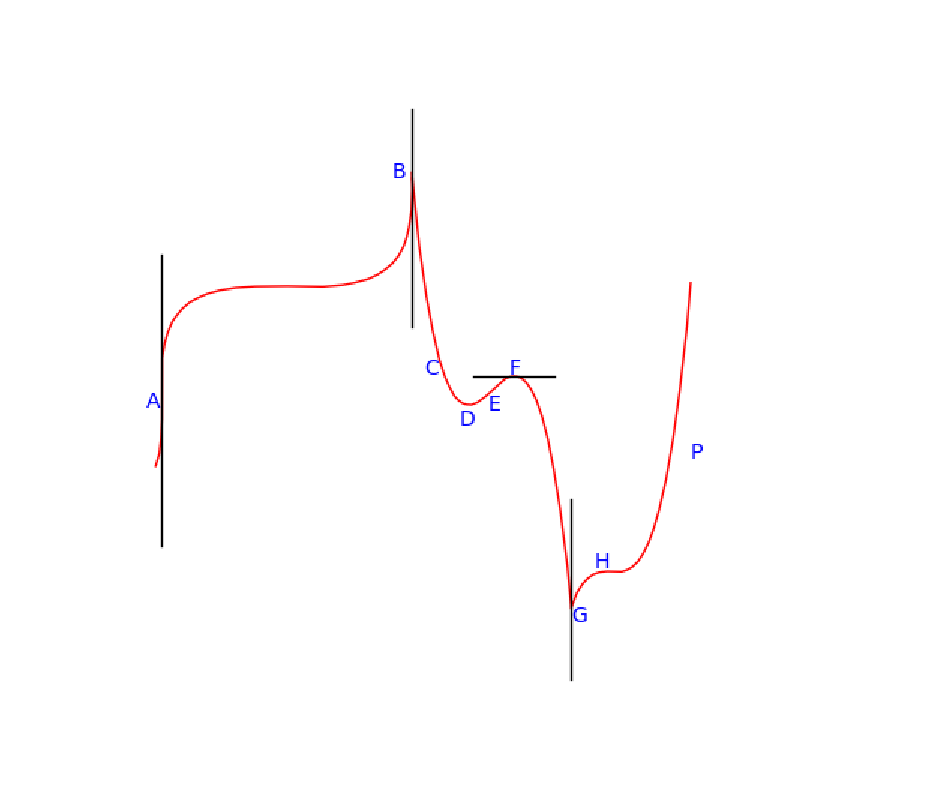
\includegraphics[height=6cm,width=12cm]{curve-tangent.eps}%
\lthtmlpictureZ
\lthtmlcheckvsize\clearpage}

{\newpage\clearpage
\lthtmlinlinemathA{tex2html_wrap_indisplay48496}%
$\displaystyle \frac{dy}{dx}\  =\  \tan\  \tau\  =\  {\rm slope\  of\  line\  
tangent\  to\  the\  curve\  at\  any\  point\  } P.
$%
\lthtmlindisplaymathZ
\lthtmlcheckvsize\clearpage}

{\newpage\clearpage
\lthtmlinlinemathA{tex2html_wrap_indisplay48498}%
$\displaystyle \frac{dy}{dx}\  =\  \tan\  \tau\  = \  {\rm slope\  of\  the\  
curve\  at\  any\  point\  } P. 
$%
\lthtmlindisplaymathZ
\lthtmlcheckvsize\clearpage}

{\newpage\clearpage
\lthtmlinlinemathA{tex2html_wrap_indisplay48500}%
$\displaystyle \left [ \frac{dy}{dx} \right ]_{x=x_1, y=y_1}\  = 
\  {\rm slope\  of\  the\  curve\  (or\  tangent)\  at\  point\  } (x_1,y_1).
$%
\lthtmlindisplaymathZ
\lthtmlcheckvsize\clearpage}

{\newpage\clearpage
\lthtmlinlinemathA{tex2html_wrap_inline48504}%
$ \tau = 0^o$%
\lthtmlinlinemathZ
\lthtmlcheckvsize\clearpage}

{\newpage\clearpage
\lthtmlinlinemathA{tex2html_wrap_inline48510}%
$ \tau = 90^o$%
\lthtmlinlinemathZ
\lthtmlcheckvsize\clearpage}

{\newpage\clearpage
\lthtmlinlinemathA{tex2html_wrap_inline48512}%
$ \frac{dy}{dx} = \infty$%
\lthtmlinlinemathZ
\lthtmlcheckvsize\clearpage}

{\newpage\clearpage
\lthtmlinlinemathA{tex2html_wrap_indisplay48516}%
$\displaystyle \tau \  = \  {\rm an\  acute\  angle;\  therefore\  }
\frac{dy}{dx}\  =\  {\rm a\  positive\  number}.
$%
\lthtmlindisplaymathZ
\lthtmlcheckvsize\clearpage}

{\newpage\clearpage
\lthtmlinlinemathA{tex2html_wrap_indisplay48518}%
$\displaystyle \tau \  = \  {\rm an\  obtuse\  angle;\  therefore\  }
\frac{dy}{dx}\  =\  {\rm a\  negative\  number}.
$%
\lthtmlindisplaymathZ
\lthtmlcheckvsize\clearpage}

{\newpage\clearpage
\lthtmlinlinemathA{tex2html_wrap_inline48527}%
$ \tau$%
\lthtmlinlinemathZ
\lthtmlcheckvsize\clearpage}

{\newpage\clearpage
\lthtmlinlinemathA{tex2html_wrap_inline48537}%
$ \tau = 45^o$%
\lthtmlinlinemathZ
\lthtmlcheckvsize\clearpage}

{\newpage\clearpage
\lthtmlinlinemathA{tex2html_wrap_inline48539}%
$ 2x - 3y = 6$%
\lthtmlinlinemathZ
\lthtmlcheckvsize\clearpage}

{\newpage\clearpage
\lthtmlpictureA{tex2html_wrap48541}%

% latex2html id marker 48541
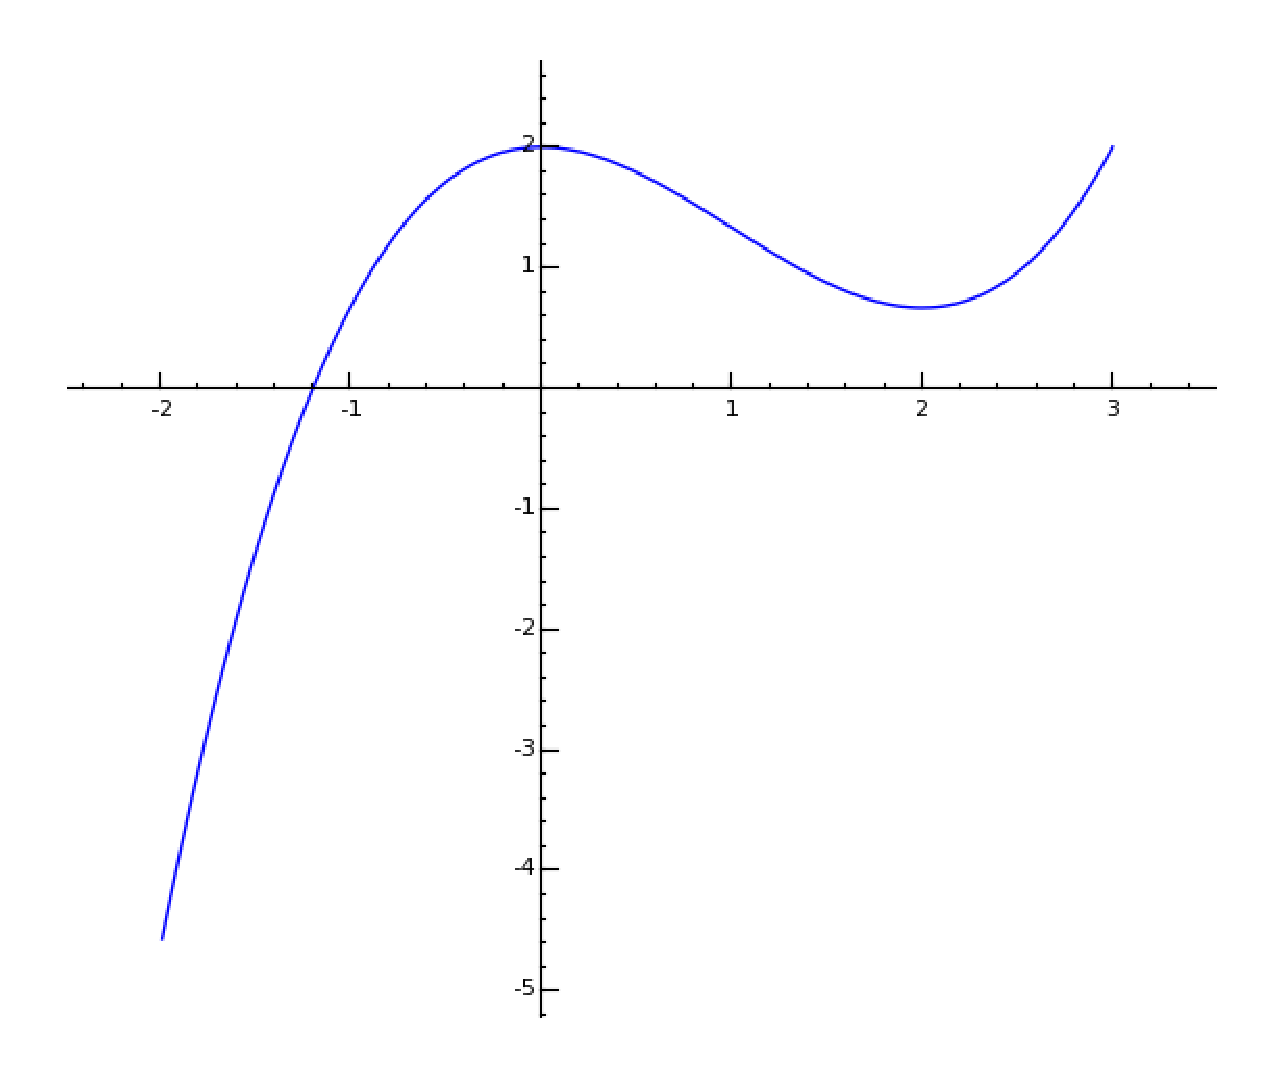
\includegraphics[height=5cm,width=7cm]{tangent-examples2.eps}%
\lthtmlpictureZ
\lthtmlcheckvsize\clearpage}

{\newpage\clearpage
\lthtmlinlinemathA{tex2html_wrap_inline48550}%
$ \frac{dy}{dx} = x^2 - 2x$%
\lthtmlinlinemathZ
\lthtmlcheckvsize\clearpage}

{\newpage\clearpage
\lthtmlinlinemathA{tex2html_wrap_inline48552}%
$ \tan \tau = \left [ \frac{dy}{dx} \right ]_{x=1} = 1 - 2 = -1$%
\lthtmlinlinemathZ
\lthtmlcheckvsize\clearpage}

{\newpage\clearpage
\lthtmlinlinemathA{tex2html_wrap_inline48554}%
$ \tau = 135^o
=3\pi/4$%
\lthtmlinlinemathZ
\lthtmlcheckvsize\clearpage}

{\newpage\clearpage
\lthtmlinlinemathA{tex2html_wrap_inline48556}%
$ \tan \tau = \left [ \frac{dy}{dx} \right ]_{x=3} = 9 - 6 = 3$%
\lthtmlinlinemathZ
\lthtmlcheckvsize\clearpage}

{\newpage\clearpage
\lthtmlinlinemathA{tex2html_wrap_inline48558}%
$ \tau = \arctan\, 3 = 1.249...$%
\lthtmlinlinemathZ
\lthtmlcheckvsize\clearpage}

{\newpage\clearpage
\lthtmlinlinemathA{tex2html_wrap_inline48562}%
$ \tan \tau = \frac{dy}{dx} = 0$%
\lthtmlinlinemathZ
\lthtmlcheckvsize\clearpage}

{\newpage\clearpage
\lthtmlinlinemathA{tex2html_wrap_inline48564}%
$ x^2 - 2x = 0$%
\lthtmlinlinemathZ
\lthtmlcheckvsize\clearpage}

{\newpage\clearpage
\lthtmlinlinemathA{tex2html_wrap_inline48574}%
$ \tan \tau = \frac{dy}{dx} = 1$%
\lthtmlinlinemathZ
\lthtmlcheckvsize\clearpage}

{\newpage\clearpage
\lthtmlinlinemathA{tex2html_wrap_inline48576}%
$ x^2 - 2x = 1$%
\lthtmlinlinemathZ
\lthtmlcheckvsize\clearpage}

{\newpage\clearpage
\lthtmlinlinemathA{tex2html_wrap_inline48578}%
$ x = 1 \pm \sqrt{2}$%
\lthtmlinlinemathZ
\lthtmlcheckvsize\clearpage}

{\newpage\clearpage
\lthtmlinlinemathA{tex2html_wrap_inline48582}%
$ x^2 - 2x = \frac{2}{3}$%
\lthtmlinlinemathZ
\lthtmlcheckvsize\clearpage}

{\newpage\clearpage
\lthtmlinlinemathA{tex2html_wrap_inline48584}%
$ x = 1 \pm \sqrt{\frac{5}{3}}$%
\lthtmlinlinemathZ
\lthtmlcheckvsize\clearpage}

{\newpage\clearpage
\lthtmlinlinemathA{tex2html_wrap_inline48597}%
$ (3, 2)$%
\lthtmlinlinemathZ
\lthtmlcheckvsize\clearpage}

{\newpage\clearpage
\lthtmlinlinemathA{tex2html_wrap_inline48599}%
$ (1, -2)$%
\lthtmlinlinemathZ
\lthtmlcheckvsize\clearpage}

{\newpage\clearpage
\lthtmlpictureA{tex2html_wrap48601}%
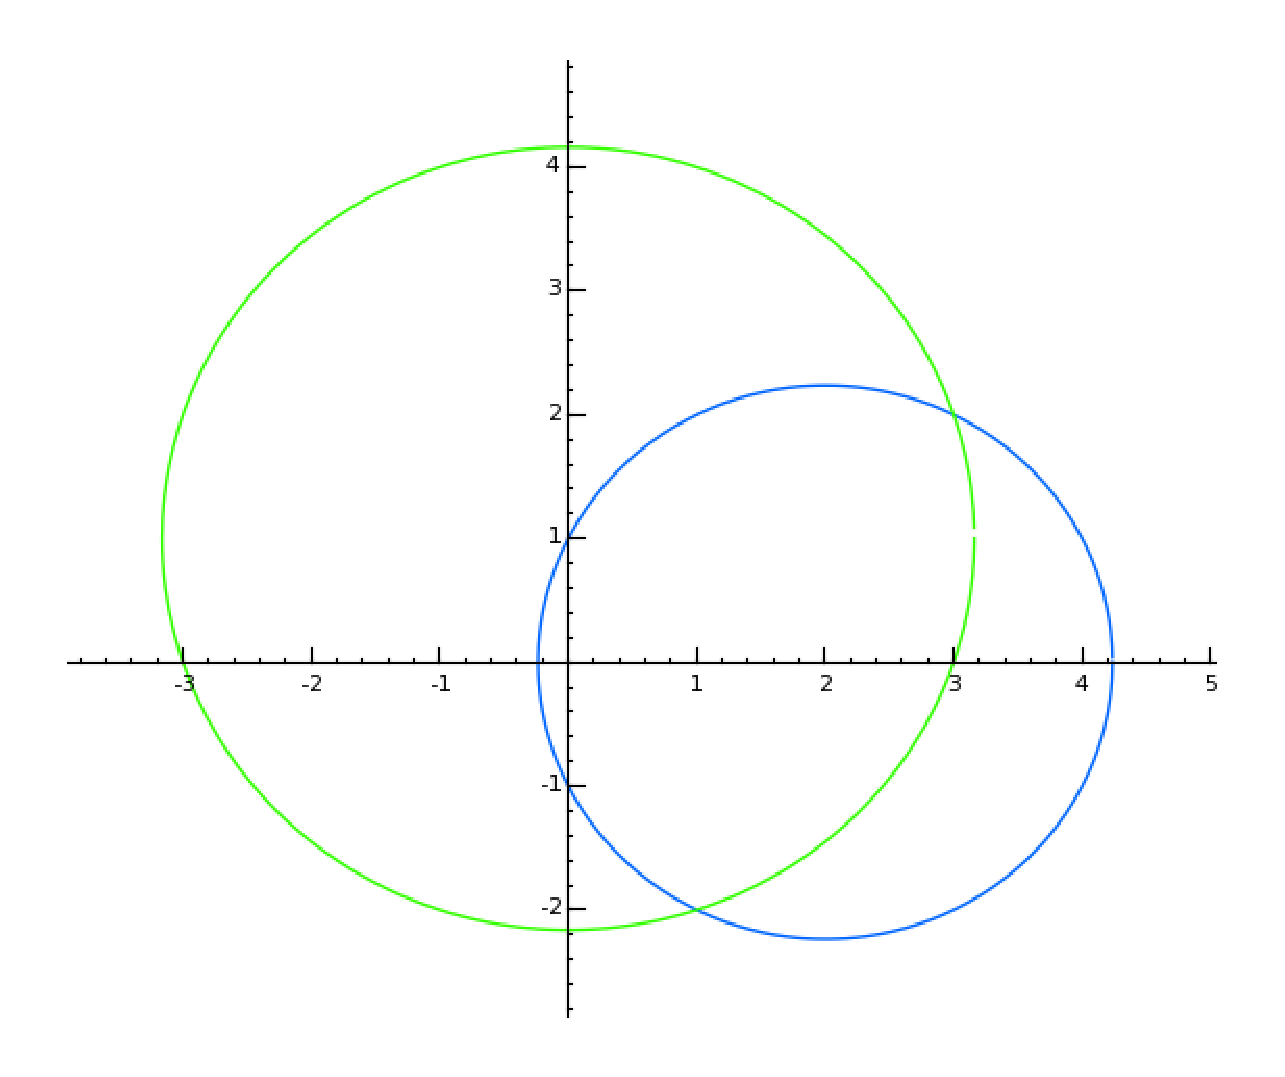
\includegraphics[height=5cm,width=6cm]{circles.eps}%
\lthtmlpictureZ
\lthtmlcheckvsize\clearpage}

{\newpage\clearpage
\lthtmlinlinemathA{tex2html_wrap_inline48614}%
$ \frac{dy}{dx} 	= \frac{2 - x}{y}$%
\lthtmlinlinemathZ
\lthtmlcheckvsize\clearpage}

{\newpage\clearpage
\lthtmlinlinemathA{tex2html_wrap_inline48616}%
$ \frac{dy}{dx} 	= \frac{x}{1 - y}$%
\lthtmlinlinemathZ
\lthtmlcheckvsize\clearpage}

{\newpage\clearpage
\lthtmlinlinemathA{tex2html_wrap_indisplay48618}%
$\displaystyle \left [ \frac{2 - x}{y} \right ]_{x = 3, y = 2} 	
= -\frac{1}{2} =\  {\rm slope\  of\  tangent\  to\  (A)\  at\  } (3, 2).
$%
\lthtmlindisplaymathZ
\lthtmlcheckvsize\clearpage}

{\newpage\clearpage
\lthtmlinlinemathA{tex2html_wrap_indisplay48620}%
$\displaystyle \left [ \frac{x}{1 - y} \right ]_{x = 3, y = 2} 	= - 3 
=\  {\rm slope\  of\  tangent\  to\  (B)\  at\  }(3, 2).
$%
\lthtmlindisplaymathZ
\lthtmlcheckvsize\clearpage}

{\newpage\clearpage
\lthtmlinlinemathA{tex2html_wrap_indisplay48626}%
$\displaystyle \tan\theta = \frac{m_1 - m_2}{1 + m_1 m_2},
$%
\lthtmlindisplaymathZ
\lthtmlcheckvsize\clearpage}

{\newpage\clearpage
\lthtmlinlinemathA{tex2html_wrap_inline48628}%
$ \tan \theta = \frac{-\frac{1}{2} + 3}{1 + \frac{3}{2}} = 1$%
\lthtmlinlinemathZ
\lthtmlcheckvsize\clearpage}

{\newpage\clearpage
\lthtmlinlinemathA{tex2html_wrap_inline48630}%
$ \theta = \pi/4= 45^o$%
\lthtmlinlinemathZ
\lthtmlcheckvsize\clearpage}

\stepcounter{section}
{\newpage\clearpage
\lthtmlinlinemathA{tex2html_wrap_inline48635}%
$ y = \frac{x}{1 + x^2}$%
\lthtmlinlinemathZ
\lthtmlcheckvsize\clearpage}

{\newpage\clearpage
\lthtmlinlinemathA{tex2html_wrap_inline48637}%
$ 1 = \tan\, \tau$%
\lthtmlinlinemathZ
\lthtmlcheckvsize\clearpage}

{\newpage\clearpage
\lthtmlinlinemathA{tex2html_wrap_inline48639}%
$ x^2y^2 = a^3(x + y)$%
\lthtmlinlinemathZ
\lthtmlcheckvsize\clearpage}

{\newpage\clearpage
\lthtmlinlinemathA{tex2html_wrap_inline48645}%
$ y = 3x^2 - x$%
\lthtmlinlinemathZ
\lthtmlcheckvsize\clearpage}

{\newpage\clearpage
\lthtmlinlinemathA{tex2html_wrap_inline48653}%
$ y = x^3 - 3x^2 - 9x + 5$%
\lthtmlinlinemathZ
\lthtmlcheckvsize\clearpage}

{\newpage\clearpage
\lthtmlinlinemathA{tex2html_wrap_inline48661}%
$ y^2 = 2x^3$%
\lthtmlinlinemathZ
\lthtmlcheckvsize\clearpage}

{\newpage\clearpage
\lthtmlinlinemathA{tex2html_wrap_inline48665}%
$ (2, 4)$%
\lthtmlinlinemathZ
\lthtmlcheckvsize\clearpage}

{\newpage\clearpage
\lthtmlinlinemathA{tex2html_wrap_inline48669}%
$ -\frac{3}{4}$%
\lthtmlinlinemathZ
\lthtmlcheckvsize\clearpage}

{\newpage\clearpage
\lthtmlinlinemathA{tex2html_wrap_inline48671}%
$ \left ( \pm \frac{3r}{5}, \pm \frac{4r}{5} \right )$%
\lthtmlinlinemathZ
\lthtmlcheckvsize\clearpage}

{\newpage\clearpage
\lthtmlinlinemathA{tex2html_wrap_inline48673}%
$ y = x^2 - 7x + 3$%
\lthtmlinlinemathZ
\lthtmlcheckvsize\clearpage}

{\newpage\clearpage
\lthtmlinlinemathA{tex2html_wrap_inline48675}%
$ y = 5x + 2$%
\lthtmlinlinemathZ
\lthtmlcheckvsize\clearpage}

{\newpage\clearpage
\lthtmlinlinemathA{tex2html_wrap_inline48677}%
$ (6, -3)$%
\lthtmlinlinemathZ
\lthtmlcheckvsize\clearpage}

{\newpage\clearpage
\lthtmlinlinemathA{tex2html_wrap_inline48679}%
$ x^2 + y^2 = 169$%
\lthtmlinlinemathZ
\lthtmlcheckvsize\clearpage}

{\newpage\clearpage
\lthtmlinlinemathA{tex2html_wrap_inline48681}%
$ 5x + 12y = 60$%
\lthtmlinlinemathZ
\lthtmlcheckvsize\clearpage}

{\newpage\clearpage
\lthtmlinlinemathA{tex2html_wrap_inline48683}%
$ (\pm 12, \mp 5)$%
\lthtmlinlinemathZ
\lthtmlcheckvsize\clearpage}

{\newpage\clearpage
\lthtmlinlinemathA{tex2html_wrap_inline48685}%
$ y = \log\, kx$%
\lthtmlinlinemathZ
\lthtmlcheckvsize\clearpage}

{\newpage\clearpage
\lthtmlinlinemathA{tex2html_wrap_inline48689}%
$ y = 2x - x^2$%
\lthtmlinlinemathZ
\lthtmlcheckvsize\clearpage}

{\newpage\clearpage
\lthtmlinlinemathA{tex2html_wrap_inline48695}%
$ \frac{3}{2}$%
\lthtmlinlinemathZ
\lthtmlcheckvsize\clearpage}

{\newpage\clearpage
\lthtmlinlinemathA{tex2html_wrap_inline48697}%
$ 45^o=\pi/4$%
\lthtmlinlinemathZ
\lthtmlcheckvsize\clearpage}

{\newpage\clearpage
\lthtmlinlinemathA{tex2html_wrap_inline48699}%
$ \arctan\, 2$%
\lthtmlinlinemathZ
\lthtmlcheckvsize\clearpage}

{\newpage\clearpage
\lthtmlinlinemathA{tex2html_wrap_inline48701}%
$ 135^o=3\pi/4$%
\lthtmlinlinemathZ
\lthtmlcheckvsize\clearpage}

{\newpage\clearpage
\lthtmlinlinemathA{tex2html_wrap_inline48703}%
$ (\frac{1}{2}, \frac{3}{4})$%
\lthtmlinlinemathZ
\lthtmlcheckvsize\clearpage}

{\newpage\clearpage
\lthtmlinlinemathA{tex2html_wrap_inline48705}%
$ (1, 1)$%
\lthtmlinlinemathZ
\lthtmlcheckvsize\clearpage}

{\newpage\clearpage
\lthtmlinlinemathA{tex2html_wrap_inline48711}%
$ 3y - 2x - 8 = 0$%
\lthtmlinlinemathZ
\lthtmlcheckvsize\clearpage}

{\newpage\clearpage
\lthtmlinlinemathA{tex2html_wrap_inline48713}%
$ y^2 = 8x$%
\lthtmlinlinemathZ
\lthtmlcheckvsize\clearpage}

{\newpage\clearpage
\lthtmlinlinemathA{tex2html_wrap_inline48715}%
$ \arctan \frac{1}{5}$%
\lthtmlinlinemathZ
\lthtmlcheckvsize\clearpage}

{\newpage\clearpage
\lthtmlinlinemathA{tex2html_wrap_inline48717}%
$ \arctan \frac{1}{8}$%
\lthtmlinlinemathZ
\lthtmlcheckvsize\clearpage}

{\newpage\clearpage
\lthtmlinlinemathA{tex2html_wrap_inline48719}%
$ y^2 = 6x$%
\lthtmlinlinemathZ
\lthtmlcheckvsize\clearpage}

{\newpage\clearpage
\lthtmlinlinemathA{tex2html_wrap_inline48721}%
$ x^2 + y^2 = 16$%
\lthtmlinlinemathZ
\lthtmlcheckvsize\clearpage}

{\newpage\clearpage
\lthtmlinlinemathA{tex2html_wrap_inline48723}%
$ \arctan \frac{5}{3} \sqrt{3}$%
\lthtmlinlinemathZ
\lthtmlcheckvsize\clearpage}

{\newpage\clearpage
\lthtmlinlinemathA{tex2html_wrap_inline48725}%
$ x^2 - y^2 = 5$%
\lthtmlinlinemathZ
\lthtmlcheckvsize\clearpage}

{\newpage\clearpage
\lthtmlinlinemathA{tex2html_wrap_inline48727}%
$ \frac{x^2}{18} + \frac{y^2}{8} = 1$%
\lthtmlinlinemathZ
\lthtmlcheckvsize\clearpage}

{\newpage\clearpage
\lthtmlinlinemathA{tex2html_wrap_inline48729}%
$ x^2 + y^2 = 8ax$%
\lthtmlinlinemathZ
\lthtmlcheckvsize\clearpage}

{\newpage\clearpage
\lthtmlinlinemathA{tex2html_wrap_inline48735}%
$ x^2 = 4ay$%
\lthtmlinlinemathZ
\lthtmlcheckvsize\clearpage}

{\newpage\clearpage
\lthtmlinlinemathA{tex2html_wrap_inline48737}%
$ y = \frac{8a^3}{x^2 + 4a^2}$%
\lthtmlinlinemathZ
\lthtmlcheckvsize\clearpage}

{\newpage\clearpage
\lthtmlinlinemathA{tex2html_wrap_inline48739}%
$ \arctan\, 3 = 71^o33' = 1.249...$%
\lthtmlinlinemathZ
\lthtmlcheckvsize\clearpage}

{\newpage\clearpage
\lthtmlinlinemathA{tex2html_wrap_inline48741}%
$ x^3 + y^3 = 3axy$%
\lthtmlinlinemathZ
\lthtmlcheckvsize\clearpage}

{\newpage\clearpage
\lthtmlinlinemathA{tex2html_wrap_inline48743}%
$ y^2 = ax$%
\lthtmlinlinemathZ
\lthtmlcheckvsize\clearpage}

{\newpage\clearpage
\lthtmlinlinemathA{tex2html_wrap_inline48747}%
$ y = x^3 - 2x^2 + x - 4$%
\lthtmlinlinemathZ
\lthtmlcheckvsize\clearpage}

{\newpage\clearpage
\lthtmlinlinemathA{tex2html_wrap_inline48751}%
$ (1,-4)$%
\lthtmlinlinemathZ
\lthtmlcheckvsize\clearpage}

{\newpage\clearpage
\lthtmlinlinemathA{tex2html_wrap_inline48753}%
$ (\frac{1}{3}, -\frac{104}{27})$%
\lthtmlinlinemathZ
\lthtmlcheckvsize\clearpage}

{\newpage\clearpage
\lthtmlinlinemathA{tex2html_wrap_inline48761}%
$ a_1x^2 + b_1y^2 = 1$%
\lthtmlinlinemathZ
\lthtmlcheckvsize\clearpage}

{\newpage\clearpage
\lthtmlinlinemathA{tex2html_wrap_inline48763}%
$ a_2x^2 + b_2y^2 = 1$%
\lthtmlinlinemathZ
\lthtmlcheckvsize\clearpage}

{\newpage\clearpage
\lthtmlinlinemathA{tex2html_wrap_inline48765}%
$ \frac{1}{a_1} - \frac{1}{b_1} = \frac{1}{b_2} - \frac{1}{b_2}$%
\lthtmlinlinemathZ
\lthtmlcheckvsize\clearpage}

\stepcounter{section}
{\newpage\clearpage
\lthtmlinlinemathA{tex2html_wrap_inline48770}%
$ m$%
\lthtmlinlinemathZ
\lthtmlcheckvsize\clearpage}

{\newpage\clearpage
\lthtmlinlinemathA{tex2html_wrap_indisplay48772}%
$\displaystyle y-y_1 = m(x-x_1)
$%
\lthtmlindisplaymathZ
\lthtmlcheckvsize\clearpage}

{\newpage\clearpage
\lthtmlpictureA{tex2html_wrap48774}%
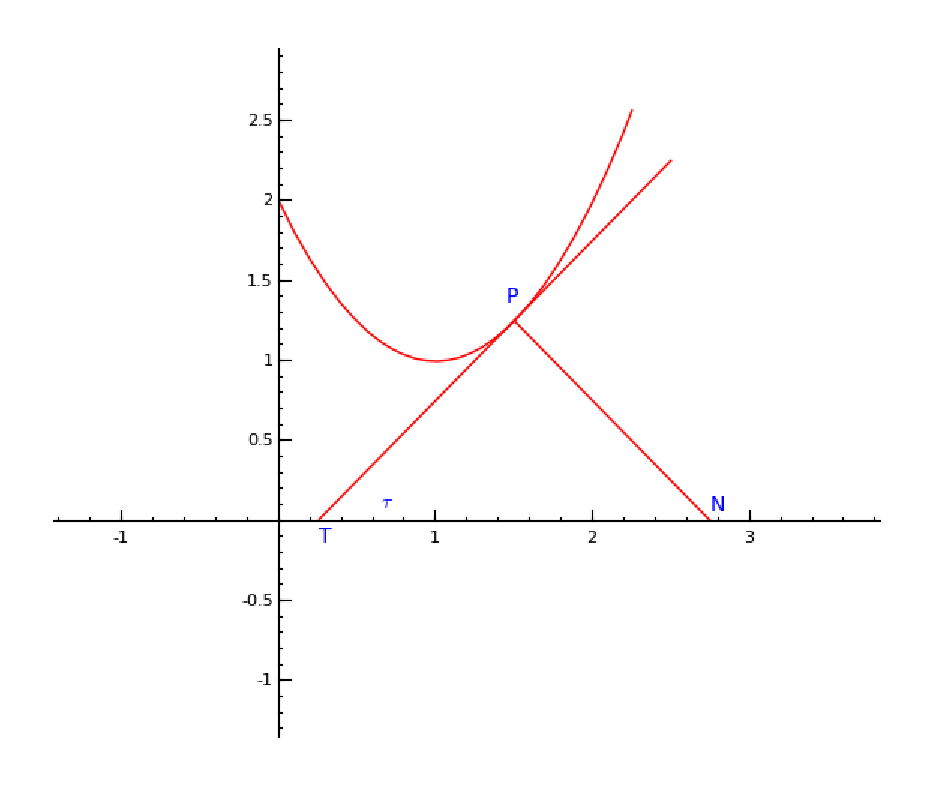
\includegraphics[height=4cm,width=6cm]{parabola-tangent2b.eps}%
\lthtmlpictureZ
\lthtmlcheckvsize\clearpage}

{\newpage\clearpage
\lthtmlinlinemathA{tex2html_wrap_inline48779}%
$ P_1(x_1,y_1)$%
\lthtmlinlinemathZ
\lthtmlcheckvsize\clearpage}

{\newpage\clearpage
\lthtmlinlinemathA{tex2html_wrap_indisplay48781}%
$\displaystyle m = \tan \tau = \left [ \frac{dy}{dx} \right ]_{x=x_1, y=y_1} 
= \frac{dy}{dx}|_{x=x_1,y=y_1}.
$%
\lthtmlindisplaymathZ
\lthtmlcheckvsize\clearpage}

{\newpage\clearpage
\lthtmlinlinemathA{tex2html_wrap_inline48785}%
$ TP_1$%
\lthtmlinlinemathZ
\lthtmlcheckvsize\clearpage}

{\newpage\clearpage
\lthtmlinlinemathA{tex2html_wrap_indisplay48787}%
$\displaystyle y - y_1 = (\frac{dy}{dx}|_{x=x_1,y=y_1})(x - x_1).$%
\lthtmlindisplaymathZ
\lthtmlcheckvsize\clearpage}

{\newpage\clearpage
\lthtmlinlinemathA{tex2html_wrap_indisplay48789}%
$\displaystyle -\frac{1}{m} 	= -\frac{dx}{dy} |_{x=x_1,y=y_1}	%By 55, p. 3 [§ 1]
$%
\lthtmlindisplaymathZ
\lthtmlcheckvsize\clearpage}

{\newpage\clearpage
\lthtmlinlinemathA{tex2html_wrap_inline48793}%
$ P_1N$%
\lthtmlinlinemathZ
\lthtmlcheckvsize\clearpage}

{\newpage\clearpage
\lthtmlinlinemathA{tex2html_wrap_indisplay48795}%
$\displaystyle y - y_1 = -(\frac{dx}{dy}|_{x=x_1,y=y_1})(x - x_1).$%
\lthtmlindisplaymathZ
\lthtmlcheckvsize\clearpage}

{\newpage\clearpage
\lthtmlinlinemathA{tex2html_wrap_inline48811}%
$ TM$%
\lthtmlinlinemathZ
\lthtmlcheckvsize\clearpage}

{\newpage\clearpage
\lthtmlinlinemathA{tex2html_wrap_inline48815}%
$ MN$%
\lthtmlinlinemathZ
\lthtmlcheckvsize\clearpage}

{\newpage\clearpage
\lthtmlinlinemathA{tex2html_wrap_inline48817}%
$ TP_1M$%
\lthtmlinlinemathZ
\lthtmlcheckvsize\clearpage}

{\newpage\clearpage
\lthtmlinlinemathA{tex2html_wrap_inline48819}%
$ \tan\, \tau = \frac{MP_1}{TM}$%
\lthtmlinlinemathZ
\lthtmlcheckvsize\clearpage}

{\newpage\clearpage
\lthtmlinlinemathA{tex2html_wrap_indisplay48823}%
$\displaystyle TM = \frac{MP_1}{\tan \tau} = y_1 \frac{dx}{dy}|_{x=x_1,y=y_1} = \  {\rm length\  of\  subtangent}.$%
\lthtmlindisplaymathZ
\lthtmlcheckvsize\clearpage}

{\newpage\clearpage
\lthtmlinlinemathA{tex2html_wrap_inline48825}%
$ MP_1N$%
\lthtmlinlinemathZ
\lthtmlcheckvsize\clearpage}

{\newpage\clearpage
\lthtmlinlinemathA{tex2html_wrap_inline48827}%
$ \tan\, \tau = \frac{MN}{MP_1}$%
\lthtmlinlinemathZ
\lthtmlcheckvsize\clearpage}

{\newpage\clearpage
\lthtmlinlinemathA{tex2html_wrap_indisplay48831}%
$\displaystyle MN =MP_1 \tan \tau = y_1 \frac{dy}{dx}|_{x=x_1,y=y_1}  = {\rm\  length\  of\  subnormal}.$%
\lthtmlindisplaymathZ
\lthtmlcheckvsize\clearpage}

{\newpage\clearpage
\lthtmlinlinemathA{tex2html_wrap_inline48833}%
$ = TP_1$%
\lthtmlinlinemathZ
\lthtmlcheckvsize\clearpage}

{\newpage\clearpage
\lthtmlinlinemathA{tex2html_wrap_inline48835}%
$ = P_1N$%
\lthtmlinlinemathZ
\lthtmlcheckvsize\clearpage}

{\newpage\clearpage
\lthtmldisplayA{displaymath48837}%
\begin{displaymath}\begin{array}{ll} TP_1  &= \sqrt{\bar{TM}^2 + \bar{MP_1}^2}\\&= \sqrt{ \left ( y_1 \frac{dx}{dy}|_{x=x_1,y=y_1} \right)^2 + (y_1)^2}\\&= y_1 \sqrt{ \left ( \frac{dx}{dy}|_{x=x_1,y=y_1} \right)^2 + 1}\\&= \  {\rm length\  of\  tangent}. \end{array}\end{displaymath}%
\lthtmldisplayZ
\lthtmlcheckvsize\clearpage}

{\newpage\clearpage
\lthtmldisplayA{displaymath48839}%
\begin{displaymath}\begin{array}{ll} P_1N  &= \sqrt{\bar{MN}^2 + \bar{MP_1}^2}\\&= \sqrt{ \left ( \frac{dy}{dx}|_{x=x_1,y=y_1} \right)^2 + (y_1)^2}\\&= y_1 \sqrt{ \left ( \frac{dy}{dx}|_{x=x_1,y=y_1} \right)^2 + 1}\\&= \  {\rm length\  of\  normal}. \end{array}\end{displaymath}%
\lthtmldisplayZ
\lthtmlcheckvsize\clearpage}

\stepcounter{section}
{\newpage\clearpage
\lthtmlinlinemathA{tex2html_wrap_inline48842}%
$ (a,a)$%
\lthtmlinlinemathZ
\lthtmlcheckvsize\clearpage}

{\newpage\clearpage
\lthtmlpictureA{tex2html_wrap48846}%
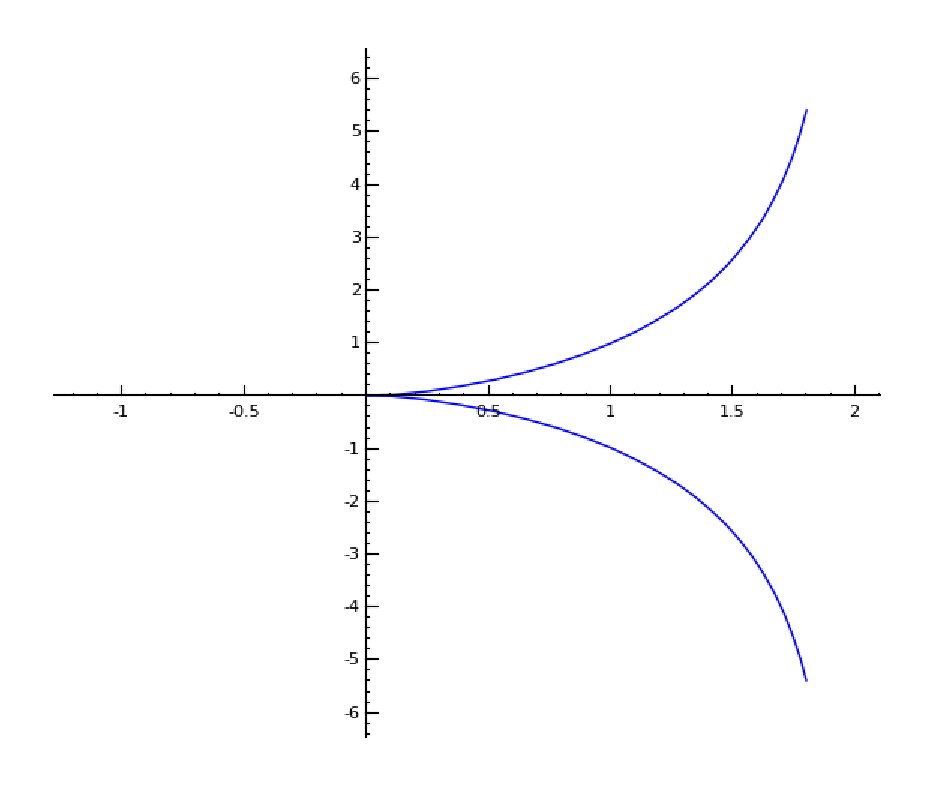
\includegraphics[height=5cm,width=5cm]{cissoid.eps}%
\lthtmlpictureZ
\lthtmlcheckvsize\clearpage}

{\newpage\clearpage
\lthtmlinlinemathA{tex2html_wrap_inline48859}%
$ \frac{dy}{dx} 	=\  \frac{3ax^2 - x^3}{y(2a - x)^2}$%
\lthtmlinlinemathZ
\lthtmlcheckvsize\clearpage}

{\newpage\clearpage
\lthtmlinlinemathA{tex2html_wrap_indisplay48861}%
$\displaystyle \frac{dy_1}{dx_1} = \left [ \frac{dy}{dx} \right ]_{x = a, y = a} 	
=\  \frac{3a^3 - a^3}{a(2a - a)^2} = 2 
$%
\lthtmlindisplaymathZ
\lthtmlcheckvsize\clearpage}

{\newpage\clearpage
\lthtmlinlinemathA{tex2html_wrap_indisplay48863}%
$\displaystyle y = 2x - a, 
$%
\lthtmlindisplaymathZ
\lthtmlcheckvsize\clearpage}

{\newpage\clearpage
\lthtmlinlinemathA{tex2html_wrap_indisplay48865}%
$\displaystyle 2y + x 	= 3a, 
$%
\lthtmlindisplaymathZ
\lthtmlcheckvsize\clearpage}

{\newpage\clearpage
\lthtmlinlinemathA{tex2html_wrap_indisplay48867}%
$\displaystyle TM 	= \frac{a}{2},
$%
\lthtmlindisplaymathZ
\lthtmlcheckvsize\clearpage}

{\newpage\clearpage
\lthtmlinlinemathA{tex2html_wrap_indisplay48869}%
$\displaystyle MN 	= 2a,
$%
\lthtmlindisplaymathZ
\lthtmlcheckvsize\clearpage}

{\newpage\clearpage
\lthtmlinlinemathA{tex2html_wrap_indisplay48871}%
$\displaystyle PT = \sqrt{(TM)^2 + (MP)^2} 
= \sqrt{\frac{a^2}{4} + a^2} 
= \frac{a}{2} \sqrt{5},
$%
\lthtmlindisplaymathZ
\lthtmlcheckvsize\clearpage}

{\newpage\clearpage
\lthtmlinlinemathA{tex2html_wrap_indisplay48873}%
$\displaystyle PN = \sqrt{(MN)^2 + (MP)^2} 
= \sqrt{4a^2 + a^2} = a \sqrt{5},
$%
\lthtmlindisplaymathZ
\lthtmlcheckvsize\clearpage}

{\newpage\clearpage
\lthtmlinlinemathA{tex2html_wrap_inline48875}%
$ x^2 + 2y^2 - 2xy - x = 0$%
\lthtmlinlinemathZ
\lthtmlcheckvsize\clearpage}

{\newpage\clearpage
\lthtmlinlinemathA{tex2html_wrap_inline48879}%
$ (1,0)$%
\lthtmlinlinemathZ
\lthtmlcheckvsize\clearpage}

{\newpage\clearpage
\lthtmlinlinemathA{tex2html_wrap_inline48881}%
$ 2y = x - 1$%
\lthtmlinlinemathZ
\lthtmlcheckvsize\clearpage}

{\newpage\clearpage
\lthtmlinlinemathA{tex2html_wrap_inline48883}%
$ y + 2x = 2$%
\lthtmlinlinemathZ
\lthtmlcheckvsize\clearpage}

{\newpage\clearpage
\lthtmlinlinemathA{tex2html_wrap_inline48887}%
$ 2y = x + 1$%
\lthtmlinlinemathZ
\lthtmlcheckvsize\clearpage}

{\newpage\clearpage
\lthtmlinlinemathA{tex2html_wrap_inline48889}%
$ y + 2x = 3$%
\lthtmlinlinemathZ
\lthtmlcheckvsize\clearpage}

{\newpage\clearpage
\lthtmlinlinemathA{tex2html_wrap_inline48897}%
$ x_lx + y_1y = r^2$%
\lthtmlinlinemathZ
\lthtmlcheckvsize\clearpage}

{\newpage\clearpage
\lthtmlinlinemathA{tex2html_wrap_inline48899}%
$ x_1y - y_1x = 0$%
\lthtmlinlinemathZ
\lthtmlcheckvsize\clearpage}

{\newpage\clearpage
\lthtmlinlinemathA{tex2html_wrap_inline48901}%
$ -x_1, -\frac{{y_1}^2}{x_1}$%
\lthtmlinlinemathZ
\lthtmlcheckvsize\clearpage}

{\newpage\clearpage
\lthtmlinlinemathA{tex2html_wrap_inline48905}%
$ 2p$%
\lthtmlinlinemathZ
\lthtmlcheckvsize\clearpage}

{\newpage\clearpage
\lthtmlinlinemathA{tex2html_wrap_inline48909}%
$ \frac{x^2}{a^2} + \frac{y^2}{b^2} = 1$%
\lthtmlinlinemathZ
\lthtmlcheckvsize\clearpage}

{\newpage\clearpage
\lthtmlinlinemathA{tex2html_wrap_inline48911}%
$ \frac{x_1x}{a^2} + \frac{y_1y}{b^2} = 1$%
\lthtmlinlinemathZ
\lthtmlcheckvsize\clearpage}

{\newpage\clearpage
\lthtmlinlinemathA{tex2html_wrap_inline48915}%
$ b=2$%
\lthtmlinlinemathZ
\lthtmlcheckvsize\clearpage}

{\newpage\clearpage
\lthtmlinlinemathA{tex2html_wrap_inline48917}%
$ x^2 + \frac{y^2}{4} = 1$%
\lthtmlinlinemathZ
\lthtmlcheckvsize\clearpage}

{\newpage\clearpage
\lthtmlinlinemathA{tex2html_wrap_inline48919}%
$ x_1=4/5$%
\lthtmlinlinemathZ
\lthtmlcheckvsize\clearpage}

{\newpage\clearpage
\lthtmlinlinemathA{tex2html_wrap_inline48921}%
$ y_1=6/5$%
\lthtmlinlinemathZ
\lthtmlcheckvsize\clearpage}

{\newpage\clearpage
\lthtmlinlinemathA{tex2html_wrap_inline48923}%
$ F(x,y)=0$%
\lthtmlinlinemathZ
\lthtmlcheckvsize\clearpage}

{\newpage\clearpage
\lthtmlinlinemathA{tex2html_wrap_inline48925}%
$ F_x(x,y)+\frac{dy}{dx}F_y(x,y)=0$%
\lthtmlinlinemathZ
\lthtmlcheckvsize\clearpage}

{\newpage\clearpage
\lthtmlinlinemathA{tex2html_wrap_indisplay48931}%
$\displaystyle {\rm length\  of\  subtangent} = y_1 \frac{dx}{dy}|_{x=x_1,y=y_1} =
(6/5)(-3/8)=-9/20,
$%
\lthtmlindisplaymathZ
\lthtmlcheckvsize\clearpage}

{\newpage\clearpage
\lthtmlinlinemathA{tex2html_wrap_indisplay48933}%
$\displaystyle {\rm\  length\  of\  subnormal}
= y_1 \frac{dy}{dx}|_{x=x_1,y=y_1} = (6/5)(-8/3)=-16/5,
$%
\lthtmlindisplaymathZ
\lthtmlcheckvsize\clearpage}

{\newpage\clearpage
\lthtmldisplayA{displaymath48935}%
\begin{displaymath}
\begin{array}{ll}
{\rm length\  of\  tangent}
=y_1 \sqrt{ \left ( \frac{dx}{dy}|_{x=x_1,y=y_1} \right)^2 + 1}
&= (6/5)\sqrt{1+\frac{9}{64}}\\
&=3\sqrt{73}/20
=1.2816...\  ,
\end{array}
\end{displaymath}%
\lthtmldisplayZ
\lthtmlcheckvsize\clearpage}

{\newpage\clearpage
\lthtmldisplayA{displaymath48937}%
\begin{displaymath}
\begin{array}{ll}
{\rm length\  of\  normal}
= y_1 \sqrt{ \left ( \frac{dy}{dx}|_{x=x_1,y=y_1} \right)^2 + 1}
&=(6/5)\sqrt{1+\frac{64}{9}}\\
&=2\sqrt{73}/5
=3.4176...\  .
\end{array}
\end{displaymath}%
\lthtmldisplayZ
\lthtmlcheckvsize\clearpage}

{\newpage\clearpage
\lthtmlinlinemathA{tex2html_wrap_inline48939}%
$ y = \frac{8a^3}{4a^2 + x^2}$%
\lthtmlinlinemathZ
\lthtmlcheckvsize\clearpage}

{\newpage\clearpage
\lthtmlinlinemathA{tex2html_wrap_inline48941}%
$ x = 2a$%
\lthtmlinlinemathZ
\lthtmlcheckvsize\clearpage}

{\newpage\clearpage
\lthtmlinlinemathA{tex2html_wrap_inline48943}%
$ x + 2y = 4a$%
\lthtmlinlinemathZ
\lthtmlcheckvsize\clearpage}

{\newpage\clearpage
\lthtmlinlinemathA{tex2html_wrap_inline48945}%
$ y = 2x - 3a$%
\lthtmlinlinemathZ
\lthtmlcheckvsize\clearpage}

{\newpage\clearpage
\lthtmlinlinemathA{tex2html_wrap_inline48947}%
$ y = \frac{a}{2}(e^{\frac{x}{a}} + e^{-\frac{x}{a}})$%
\lthtmlinlinemathZ
\lthtmlcheckvsize\clearpage}

{\newpage\clearpage
\lthtmlinlinemathA{tex2html_wrap_inline48949}%
$ \frac{a}{4}(e^{\frac{2x}{a}} - e^{-\frac{2x}{a}})$%
\lthtmlinlinemathZ
\lthtmlcheckvsize\clearpage}

{\newpage\clearpage
\lthtmlinlinemathA{tex2html_wrap_inline48951}%
$ \frac{y^2}{a}$%
\lthtmlinlinemathZ
\lthtmlcheckvsize\clearpage}

{\newpage\clearpage
\lthtmldisplayA{displaymath48953}%
\begin{displaymath}
\begin{array}{ll}
(a)\  \  y = x^3\  {\rm at}\  
(\frac{1}{2}, \frac{1}{8}) & 	(e)\  \  y = 9-x^2 \  {\rm at}\  (-3,0)\\
 & \\
(b)\  \  y^2 = 4x \  {\rm at}\   (9,-6) & 	(f)\  \  x^2 = 6y \  {\rm where}\  x = -6\\
 & \\
(c)\  \  x^2 + 5y^2 = 14\  {\rm where}\   y = 1 &	(g)\  \  x^2 - xy + 2x - 9 = 0\  {\rm at}\  (3,2)\\
 & \\
(d)\  \  x^2 + y^2 = 25 at (-3,-4)  & (h)\  \  2x^2 - y^2 = 14\  {\rm at}\  (3,-2)
\end{array}
\end{displaymath}%
\lthtmldisplayZ
\lthtmlcheckvsize\clearpage}

{\newpage\clearpage
\lthtmlinlinemathA{tex2html_wrap_inline48957}%
$ \frac{1}{\log a}$%
\lthtmlinlinemathZ
\lthtmlcheckvsize\clearpage}

{\newpage\clearpage
\lthtmlinlinemathA{tex2html_wrap_inline48959}%
$ y^2 = 20x$%
\lthtmlinlinemathZ
\lthtmlcheckvsize\clearpage}

{\newpage\clearpage
\lthtmlinlinemathA{tex2html_wrap_inline48965}%
$ y = x + 5$%
\lthtmlinlinemathZ
\lthtmlcheckvsize\clearpage}

{\newpage\clearpage
\lthtmlinlinemathA{tex2html_wrap_inline48967}%
$ x^2 + y^2 = 52$%
\lthtmlinlinemathZ
\lthtmlcheckvsize\clearpage}

{\newpage\clearpage
\lthtmlinlinemathA{tex2html_wrap_inline48969}%
$ 2x + 3y = 6$%
\lthtmlinlinemathZ
\lthtmlcheckvsize\clearpage}

{\newpage\clearpage
\lthtmlinlinemathA{tex2html_wrap_inline48971}%
$ 2x + 3y \pm 26 = 0$%
\lthtmlinlinemathZ
\lthtmlcheckvsize\clearpage}

{\newpage\clearpage
\lthtmlinlinemathA{tex2html_wrap_inline48973}%
$ 4x^2 - 9y^2 + 36 = 0$%
\lthtmlinlinemathZ
\lthtmlcheckvsize\clearpage}

{\newpage\clearpage
\lthtmlinlinemathA{tex2html_wrap_inline48975}%
$ 2y + 5x = 10$%
\lthtmlinlinemathZ
\lthtmlcheckvsize\clearpage}

{\newpage\clearpage
\lthtmlinlinemathA{tex2html_wrap_inline48977}%
$ 2x - 5y \pm 8 = 0$%
\lthtmlinlinemathZ
\lthtmlcheckvsize\clearpage}

{\newpage\clearpage
\lthtmlinlinemathA{tex2html_wrap_inline48979}%
$ 2xy = a^2$%
\lthtmlinlinemathZ
\lthtmlcheckvsize\clearpage}

{\newpage\clearpage
\lthtmlinlinemathA{tex2html_wrap_inline48981}%
$ a^2$%
\lthtmlinlinemathZ
\lthtmlcheckvsize\clearpage}

{\newpage\clearpage
\lthtmlinlinemathA{tex2html_wrap_inline48983}%
$ y^2 = 2x^2 - x^3$%
\lthtmlinlinemathZ
\lthtmlcheckvsize\clearpage}

{\newpage\clearpage
\lthtmlinlinemathA{tex2html_wrap_inline48993}%
$ (1,-1)$%
\lthtmlinlinemathZ
\lthtmlcheckvsize\clearpage}

{\newpage\clearpage
\lthtmlinlinemathA{tex2html_wrap_inline48995}%
$ 2y =-x-1$%
\lthtmlinlinemathZ
\lthtmlcheckvsize\clearpage}

{\newpage\clearpage
\lthtmlinlinemathA{tex2html_wrap_inline48997}%
$ y-2x = -3$%
\lthtmlinlinemathZ
\lthtmlcheckvsize\clearpage}

{\newpage\clearpage
\lthtmlinlinemathA{tex2html_wrap_inline49001}%
$ x^2(x + y) = a^2(x-y)$%
\lthtmlinlinemathZ
\lthtmlcheckvsize\clearpage}

{\newpage\clearpage
\lthtmlinlinemathA{tex2html_wrap_inline49007}%
$ x=a\cos(t)^3$%
\lthtmlinlinemathZ
\lthtmlcheckvsize\clearpage}

{\newpage\clearpage
\lthtmlinlinemathA{tex2html_wrap_inline49009}%
$ y=a\sin(t)^3$%
\lthtmlinlinemathZ
\lthtmlcheckvsize\clearpage}

{\newpage\clearpage
\lthtmlinlinemathA{tex2html_wrap_inline49011}%
$ 0\leq t\leq 2\pi$%
\lthtmlinlinemathZ
\lthtmlcheckvsize\clearpage}

{\newpage\clearpage
\lthtmlinlinemathA{tex2html_wrap_inline49013}%
$ y = ae^{\frac{x}{c}}$%
\lthtmlinlinemathZ
\lthtmlcheckvsize\clearpage}

\stepcounter{section}
{\newpage\clearpage
\lthtmlinlinemathA{tex2html_wrap_indisplay49016}%
$\displaystyle F(x,y) = 0.$%
\lthtmlindisplaymathZ
\lthtmlcheckvsize\clearpage}

{\newpage\clearpage
\lthtmlinlinemathA{tex2html_wrap_inline49020}%
$ t$%
\lthtmlinlinemathZ
\lthtmlcheckvsize\clearpage}

{\newpage\clearpage
\lthtmldisplayA{displaymath49030}%
\begin{displaymath}\begin{cases}  x = f(t), \\y = g(t)  \end{cases}\end{displaymath}%
\lthtmldisplayZ
\lthtmlcheckvsize\clearpage}

{\newpage\clearpage
\lthtmlinlinemathA{tex2html_wrap_indisplay49045}%
$\displaystyle x^2 + y^2= r^2\  {\rm or}\   y = \sqrt{r^2 - x^2}.
$%
\lthtmlindisplaymathZ
\lthtmlcheckvsize\clearpage}

{\newpage\clearpage
\lthtmldisplayA{displaymath49047}%
\begin{displaymath}\begin{cases}  x= r\cos\, t \\y  = r\sin\, t \end{cases}\end{displaymath}%
\lthtmldisplayZ
\lthtmlcheckvsize\clearpage}

{\newpage\clearpage
\lthtmlinlinemathA{tex2html_wrap_inline49053}%
$ x=\frac{\sqrt{2t}}{\sqrt{1+t^2}}$%
\lthtmlinlinemathZ
\lthtmlcheckvsize\clearpage}

{\newpage\clearpage
\lthtmlinlinemathA{tex2html_wrap_inline49055}%
$ y=\frac{1-t}{\sqrt{1+t^2}}$%
\lthtmlinlinemathZ
\lthtmlcheckvsize\clearpage}

{\newpage\clearpage
\lthtmlinlinemathA{tex2html_wrap_indisplay49059}%
$\displaystyle x^2 + y^2 = r^2(\cos^2t + \sin^2t) = r^2,
$%
\lthtmlindisplaymathZ
\lthtmlcheckvsize\clearpage}

{\newpage\clearpage
\lthtmlinlinemathA{tex2html_wrap_inline49066}%
$ P(x,y)$%
\lthtmlinlinemathZ
\lthtmlcheckvsize\clearpage}

{\newpage\clearpage
\lthtmldisplayA{displaymath49079}%
\begin{displaymath}
\begin{cases} 
x = v_0 \cos \alpha \cdot t, \\
y = -\frac{1}{2} gt^2 + v_0 \sin \alpha \cdot t 
\end{cases}
\end{displaymath}%
\lthtmldisplayZ
\lthtmlcheckvsize\clearpage}

{\newpage\clearpage
\lthtmlinlinemathA{tex2html_wrap_indisplay49087}%
$\displaystyle y = x \tan \alpha - \frac{gx^2}{2v_0^2 \cos^2 \alpha}.
$%
\lthtmlindisplaymathZ
\lthtmlcheckvsize\clearpage}

{\newpage\clearpage
\lthtmldisplayA{displaymath49097}%
\begin{displaymath}
\begin{array}{ll}
\frac{dy}{dx} 
&	= \frac{dy}{dt} \cdot \frac{dt}{dx}
\  \ \  {\rm by\  XXV}\\
& 
= \frac{dy}{dt} \cdot \frac{1}{\frac{dx}{dt}}\  \ \  {\rm by\  XXVI}
\end{array}
\end{displaymath}%
\lthtmldisplayZ
\lthtmlcheckvsize\clearpage}

{\newpage\clearpage
\lthtmlinlinemathA{tex2html_wrap_indisplay49099}%
$\displaystyle \frac{dy}{dx} 	= \frac{\frac{dy}{dt}}{\frac{dx}{dt}}  = \frac{g'(t)}{f'(t)}.$%
\lthtmlindisplaymathZ
\lthtmlcheckvsize\clearpage}

{\newpage\clearpage
\lthtmldisplayA{displaymath49108}%
\begin{displaymath}\begin{cases}  x = a \cos \phi, \\y = b \sin \phi,  \end{cases}\end{displaymath}%
\lthtmldisplayZ
\lthtmlcheckvsize\clearpage}

{\newpage\clearpage
\lthtmlinlinemathA{tex2html_wrap_inline49110}%
$ \phi = \frac{\pi}{4}$%
\lthtmlinlinemathZ
\lthtmlcheckvsize\clearpage}

{\newpage\clearpage
\lthtmlinlinemathA{tex2html_wrap_inline49114}%
$ x = OA = OB\cos\phi = a\cos\phi$%
\lthtmlinlinemathZ
\lthtmlcheckvsize\clearpage}

{\newpage\clearpage
\lthtmlinlinemathA{tex2html_wrap_inline49116}%
$ y = AP = OD = OC\sin\phi = b\sin\phi$%
\lthtmlinlinemathZ
\lthtmlcheckvsize\clearpage}

{\newpage\clearpage
\lthtmlinlinemathA{tex2html_wrap_inline49118}%
$ \frac{x}{a} = \cos \phi$%
\lthtmlinlinemathZ
\lthtmlcheckvsize\clearpage}

{\newpage\clearpage
\lthtmlinlinemathA{tex2html_wrap_inline49120}%
$ \frac{y}{b} = \sin \phi$%
\lthtmlinlinemathZ
\lthtmlcheckvsize\clearpage}

{\newpage\clearpage
\lthtmlinlinemathA{tex2html_wrap_indisplay49122}%
$\displaystyle \frac{x^2}{a^2} + \frac{y^2}{b^2} = \cos^2 \phi + \sin^2 \phi = 1,
$%
\lthtmlindisplaymathZ
\lthtmlcheckvsize\clearpage}

{\newpage\clearpage
\lthtmlpictureA{tex2html_wrap49126}%
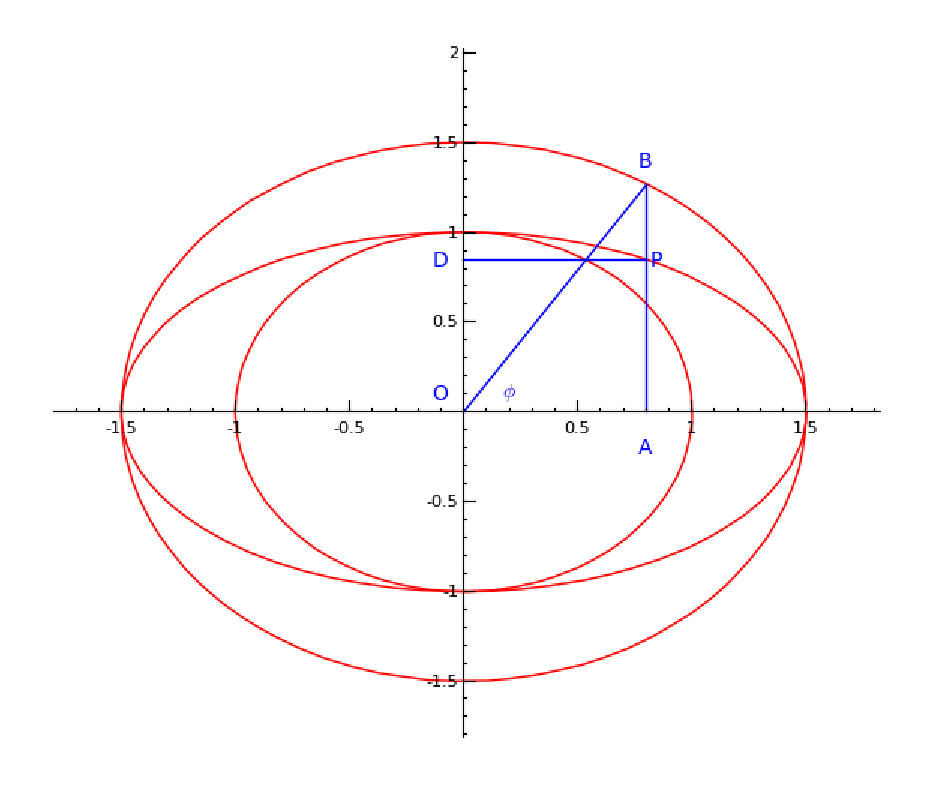
\includegraphics[height=6cm,width=6cm]{ellipse2.eps}%
\lthtmlpictureZ
\lthtmlcheckvsize\clearpage}

{\newpage\clearpage
\lthtmlinlinemathA{tex2html_wrap_inline49133}%
$ \frac{dx}{d\phi} = - a \sin \phi$%
\lthtmlinlinemathZ
\lthtmlcheckvsize\clearpage}

{\newpage\clearpage
\lthtmlinlinemathA{tex2html_wrap_inline49135}%
$ \frac{dy}{d\phi} = b \cos \phi$%
\lthtmlinlinemathZ
\lthtmlcheckvsize\clearpage}

{\newpage\clearpage
\lthtmlinlinemathA{tex2html_wrap_inline49139}%
$ \left ( \frac{a}{\sqrt{2}}, \frac{b}{\sqrt{2}} \right )$%
\lthtmlinlinemathZ
\lthtmlcheckvsize\clearpage}

{\newpage\clearpage
\lthtmlinlinemathA{tex2html_wrap_inline49141}%
$ \frac{dy}{dx}|_{x=x_1,y=y_1} = - \frac{b}{a}$%
\lthtmlinlinemathZ
\lthtmlcheckvsize\clearpage}

{\newpage\clearpage
\lthtmlinlinemathA{tex2html_wrap_indisplay49143}%
$\displaystyle y - \frac{b}{\sqrt{2}} = -\frac{b}{a} \left ( x - \frac{a}{\sqrt{2}} \right ),
$%
\lthtmlindisplaymathZ
\lthtmlcheckvsize\clearpage}

{\newpage\clearpage
\lthtmlinlinemathA{tex2html_wrap_inline49145}%
$ bx + ay = \sqrt{2} ab$%
\lthtmlinlinemathZ
\lthtmlcheckvsize\clearpage}

{\newpage\clearpage
\lthtmlinlinemathA{tex2html_wrap_indisplay49147}%
$\displaystyle y - \frac{b}{\sqrt{2}} 	= \frac{a}{b} \left ( x - \frac{a}{\sqrt{2}} \right ),
$%
\lthtmlindisplaymathZ
\lthtmlcheckvsize\clearpage}

{\newpage\clearpage
\lthtmlinlinemathA{tex2html_wrap_inline49149}%
$ \sqrt{2}(ax - by)=	a^2 - b^2$%
\lthtmlinlinemathZ
\lthtmlcheckvsize\clearpage}

{\newpage\clearpage
\lthtmlinlinemathA{tex2html_wrap_indisplay49151}%
$\displaystyle \frac{b}{\sqrt{2}} \left ( -\frac{b}{a} \right ) 
= -\frac{b^2}{a\sqrt{2}}
,$%
\lthtmlindisplaymathZ
\lthtmlcheckvsize\clearpage}

{\newpage\clearpage
\lthtmlinlinemathA{tex2html_wrap_indisplay49153}%
$\displaystyle \frac{b}{\sqrt{2}} \left ( -\frac{a}{b} \right )
= -\frac{a}{\sqrt{2}},
$%
\lthtmlindisplaymathZ
\lthtmlcheckvsize\clearpage}

{\newpage\clearpage
\lthtmldisplayA{displaymath49160}%
\begin{displaymath}
\begin{cases} 
x = a(\theta - \sin \theta), \\
y = a(1 - \cos \theta), 
\end{cases}
\end{displaymath}%
\lthtmldisplayZ
\lthtmlcheckvsize\clearpage}

{\newpage\clearpage
\lthtmlinlinemathA{tex2html_wrap_inline49164}%
$ \theta = \frac{\pi}{2}$%
\lthtmlinlinemathZ
\lthtmlcheckvsize\clearpage}

{\newpage\clearpage
\lthtmldisplayA{displaymath49170}%
\begin{displaymath}
\begin{array}{ll}
  x &= OM - NM = a\theta - a\sin\theta = a(\theta- \sin\theta),\\
    y &= PN = MC - AC = a - a\cos\theta = a(1 - \cos\theta),
\end{array}
\end{displaymath}%
\lthtmldisplayZ
\lthtmlcheckvsize\clearpage}

{\newpage\clearpage
\lthtmlinlinemathA{tex2html_wrap_inline49174}%
$ OD = 2\pi a$%
\lthtmlinlinemathZ
\lthtmlcheckvsize\clearpage}

{\newpage\clearpage
\lthtmlinlinemathA{tex2html_wrap_indisplay49178}%
$\displaystyle x = a \arccos \left ( \frac{a - y}{a} \right ) - \sqrt{ 2ay - y^2 }.
$%
\lthtmlindisplaymathZ
\lthtmlcheckvsize\clearpage}

{\newpage\clearpage
\lthtmlpictureA{tex2html_wrap49180}%
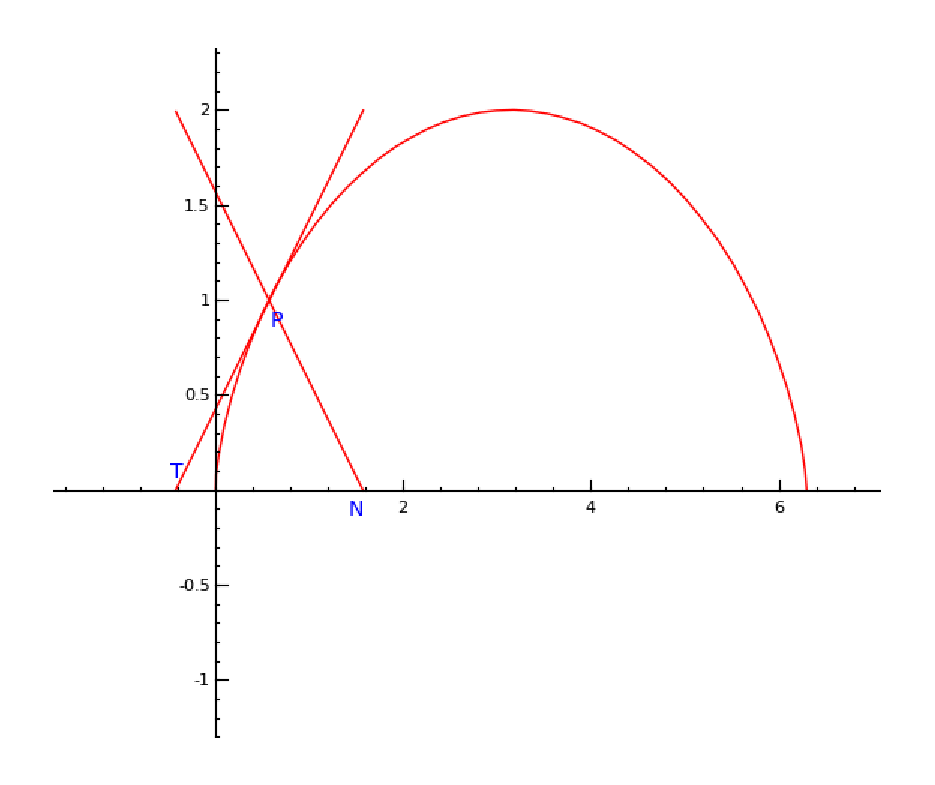
\includegraphics[height=4cm,width=8cm]{cycloid-tangent.eps}%
\lthtmlpictureZ
\lthtmlcheckvsize\clearpage}

{\newpage\clearpage
\lthtmlinlinemathA{tex2html_wrap_indisplay49185}%
$\displaystyle \frac{dx}{d\theta} 	
= a(1 - \cos \theta),\  \ \   \frac{dy}{d\theta} = a \sin \theta.
$%
\lthtmlindisplaymathZ
\lthtmlcheckvsize\clearpage}

{\newpage\clearpage
\lthtmlinlinemathA{tex2html_wrap_indisplay49187}%
$\displaystyle \frac{dy}{dx} 	= \frac{\sin \theta}{1 - \cos \theta},
$%
\lthtmlindisplaymathZ
\lthtmlcheckvsize\clearpage}

{\newpage\clearpage
\lthtmlinlinemathA{tex2html_wrap_inline49191}%
$ \left ( \frac{\pi a}{2} - a, a \right )$%
\lthtmlinlinemathZ
\lthtmlcheckvsize\clearpage}

{\newpage\clearpage
\lthtmlinlinemathA{tex2html_wrap_inline49193}%
$ \frac{dy}{dx}|_{x=x_1,y=y_1} = 1$%
\lthtmlinlinemathZ
\lthtmlcheckvsize\clearpage}

{\newpage\clearpage
\lthtmlinlinemathA{tex2html_wrap_inline49199}%
$ a \sqrt{2}$%
\lthtmlinlinemathZ
\lthtmlcheckvsize\clearpage}

\stepcounter{section}
{\newpage\clearpage
\lthtmlinlinemathA{tex2html_wrap_inline49204}%
$ x = t^2$%
\lthtmlinlinemathZ
\lthtmlcheckvsize\clearpage}

{\newpage\clearpage
\lthtmlinlinemathA{tex2html_wrap_inline49206}%
$ 2y = t$%
\lthtmlinlinemathZ
\lthtmlcheckvsize\clearpage}

{\newpage\clearpage
\lthtmlinlinemathA{tex2html_wrap_inline49208}%
$ t = 1$%
\lthtmlinlinemathZ
\lthtmlcheckvsize\clearpage}

{\newpage\clearpage
\lthtmlinlinemathA{tex2html_wrap_inline49210}%
$ x - 4y + 1 = 0$%
\lthtmlinlinemathZ
\lthtmlcheckvsize\clearpage}

{\newpage\clearpage
\lthtmlinlinemathA{tex2html_wrap_inline49212}%
$ 8x + 2y - 9 = 0$%
\lthtmlinlinemathZ
\lthtmlcheckvsize\clearpage}

{\newpage\clearpage
\lthtmlinlinemathA{tex2html_wrap_inline49216}%
$ \frac{1}{8}$%
\lthtmlinlinemathZ
\lthtmlcheckvsize\clearpage}

{\newpage\clearpage
\lthtmlinlinemathA{tex2html_wrap_inline49218}%
$ x = t$%
\lthtmlinlinemathZ
\lthtmlcheckvsize\clearpage}

{\newpage\clearpage
\lthtmlinlinemathA{tex2html_wrap_inline49220}%
$ y = t^3$%
\lthtmlinlinemathZ
\lthtmlcheckvsize\clearpage}

{\newpage\clearpage
\lthtmlinlinemathA{tex2html_wrap_inline49222}%
$ t = 2$%
\lthtmlinlinemathZ
\lthtmlcheckvsize\clearpage}

{\newpage\clearpage
\lthtmlinlinemathA{tex2html_wrap_inline49224}%
$ 12x - y - 16 = 0$%
\lthtmlinlinemathZ
\lthtmlcheckvsize\clearpage}

{\newpage\clearpage
\lthtmlinlinemathA{tex2html_wrap_inline49226}%
$ x + 12y - 98 = 0$%
\lthtmlinlinemathZ
\lthtmlcheckvsize\clearpage}

{\newpage\clearpage
\lthtmlinlinemathA{tex2html_wrap_inline49230}%
$ 96$%
\lthtmlinlinemathZ
\lthtmlcheckvsize\clearpage}

{\newpage\clearpage
\lthtmlinlinemathA{tex2html_wrap_inline49238}%
$ 3x - 2y - 1 = 0$%
\lthtmlinlinemathZ
\lthtmlcheckvsize\clearpage}

{\newpage\clearpage
\lthtmlinlinemathA{tex2html_wrap_inline49240}%
$ 2x + 3y - 5 = 0$%
\lthtmlinlinemathZ
\lthtmlcheckvsize\clearpage}

{\newpage\clearpage
\lthtmlinlinemathA{tex2html_wrap_inline49246}%
$ x = 2e^t$%
\lthtmlinlinemathZ
\lthtmlcheckvsize\clearpage}

{\newpage\clearpage
\lthtmlinlinemathA{tex2html_wrap_inline49248}%
$ y = e^{- t}$%
\lthtmlinlinemathZ
\lthtmlcheckvsize\clearpage}

{\newpage\clearpage
\lthtmlinlinemathA{tex2html_wrap_inline49250}%
$ t = 0$%
\lthtmlinlinemathZ
\lthtmlcheckvsize\clearpage}

{\newpage\clearpage
\lthtmlinlinemathA{tex2html_wrap_inline49252}%
$ x + 2y - 4 = 0$%
\lthtmlinlinemathZ
\lthtmlcheckvsize\clearpage}

{\newpage\clearpage
\lthtmlinlinemathA{tex2html_wrap_inline49254}%
$ 2x - y - 3 = 0$%
\lthtmlinlinemathZ
\lthtmlcheckvsize\clearpage}

{\newpage\clearpage
\lthtmlinlinemathA{tex2html_wrap_inline49256}%
$ -2$%
\lthtmlinlinemathZ
\lthtmlcheckvsize\clearpage}

{\newpage\clearpage
\lthtmlinlinemathA{tex2html_wrap_inline49260}%
$ x = \sin\, t$%
\lthtmlinlinemathZ
\lthtmlcheckvsize\clearpage}

{\newpage\clearpage
\lthtmlinlinemathA{tex2html_wrap_inline49262}%
$ y = \cos\, 2t$%
\lthtmlinlinemathZ
\lthtmlcheckvsize\clearpage}

{\newpage\clearpage
\lthtmlinlinemathA{tex2html_wrap_inline49264}%
$ t = \frac{\pi}{6}$%
\lthtmlinlinemathZ
\lthtmlcheckvsize\clearpage}

{\newpage\clearpage
\lthtmlinlinemathA{tex2html_wrap_inline49266}%
$ 2y + 4x - 3 = 0$%
\lthtmlinlinemathZ
\lthtmlcheckvsize\clearpage}

{\newpage\clearpage
\lthtmlinlinemathA{tex2html_wrap_inline49268}%
$ 4y - 2x - 1 = 0$%
\lthtmlinlinemathZ
\lthtmlcheckvsize\clearpage}

{\newpage\clearpage
\lthtmlinlinemathA{tex2html_wrap_inline49274}%
$ t_0=\pi/6$%
\lthtmlinlinemathZ
\lthtmlcheckvsize\clearpage}

{\newpage\clearpage
\lthtmlinlinemathA{tex2html_wrap_inline49276}%
$ (x_0,y_0)=(\sin(t_0),\cos(2t_0))=( 1/2, 1/2)$%
\lthtmlinlinemathZ
\lthtmlcheckvsize\clearpage}

{\newpage\clearpage
\lthtmlinlinemathA{tex2html_wrap_inline49278}%
$ X$%
\lthtmlinlinemathZ
\lthtmlcheckvsize\clearpage}

{\newpage\clearpage
\lthtmlinlinemathA{tex2html_wrap_inline49280}%
$ Y$%
\lthtmlinlinemathZ
\lthtmlcheckvsize\clearpage}

{\newpage\clearpage
\lthtmlinlinemathA{tex2html_wrap_inline49288}%
$ x = 1 - t$%
\lthtmlinlinemathZ
\lthtmlcheckvsize\clearpage}

{\newpage\clearpage
\lthtmlinlinemathA{tex2html_wrap_inline49290}%
$ y = t^2$%
\lthtmlinlinemathZ
\lthtmlcheckvsize\clearpage}

{\newpage\clearpage
\lthtmlinlinemathA{tex2html_wrap_inline49292}%
$ t = 3$%
\lthtmlinlinemathZ
\lthtmlcheckvsize\clearpage}

{\newpage\clearpage
\lthtmlinlinemathA{tex2html_wrap_inline49294}%
$ x = 3t$%
\lthtmlinlinemathZ
\lthtmlcheckvsize\clearpage}

{\newpage\clearpage
\lthtmlinlinemathA{tex2html_wrap_inline49296}%
$ y = 6t - t^2$%
\lthtmlinlinemathZ
\lthtmlcheckvsize\clearpage}

{\newpage\clearpage
\lthtmlinlinemathA{tex2html_wrap_inline49300}%
$ x = t^3$%
\lthtmlinlinemathZ
\lthtmlcheckvsize\clearpage}

{\newpage\clearpage
\lthtmlinlinemathA{tex2html_wrap_inline49302}%
$ y = t$%
\lthtmlinlinemathZ
\lthtmlcheckvsize\clearpage}

{\newpage\clearpage
\lthtmlinlinemathA{tex2html_wrap_inline49310}%
$ t = - 1$%
\lthtmlinlinemathZ
\lthtmlcheckvsize\clearpage}

{\newpage\clearpage
\lthtmlinlinemathA{tex2html_wrap_inline49312}%
$ x = 2 - t$%
\lthtmlinlinemathZ
\lthtmlcheckvsize\clearpage}

{\newpage\clearpage
\lthtmlinlinemathA{tex2html_wrap_inline49314}%
$ y = 3t^2$%
\lthtmlinlinemathZ
\lthtmlcheckvsize\clearpage}

{\newpage\clearpage
\lthtmlinlinemathA{tex2html_wrap_inline49318}%
$ x = \cos\, t$%
\lthtmlinlinemathZ
\lthtmlcheckvsize\clearpage}

{\newpage\clearpage
\lthtmlinlinemathA{tex2html_wrap_inline49320}%
$ y = \sin\, 2t$%
\lthtmlinlinemathZ
\lthtmlcheckvsize\clearpage}

{\newpage\clearpage
\lthtmlinlinemathA{tex2html_wrap_inline49322}%
$ t = \frac{\pi}{3}$%
\lthtmlinlinemathZ
\lthtmlcheckvsize\clearpage}

{\newpage\clearpage
\lthtmlinlinemathA{tex2html_wrap_inline49324}%
$ x = 3e^{-t}$%
\lthtmlinlinemathZ
\lthtmlcheckvsize\clearpage}

{\newpage\clearpage
\lthtmlinlinemathA{tex2html_wrap_inline49326}%
$ y = 2e^t$%
\lthtmlinlinemathZ
\lthtmlcheckvsize\clearpage}

{\newpage\clearpage
\lthtmlinlinemathA{tex2html_wrap_inline49332}%
$ y = 2 \cos\, t$%
\lthtmlinlinemathZ
\lthtmlcheckvsize\clearpage}

{\newpage\clearpage
\lthtmlinlinemathA{tex2html_wrap_inline49334}%
$ t = \frac{\pi}{4}$%
\lthtmlinlinemathZ
\lthtmlcheckvsize\clearpage}

{\newpage\clearpage
\lthtmlinlinemathA{tex2html_wrap_inline49336}%
$ x = 4 \cos\, t$%
\lthtmlinlinemathZ
\lthtmlcheckvsize\clearpage}

{\newpage\clearpage
\lthtmlinlinemathA{tex2html_wrap_inline49338}%
$ y = 3 \sin\, t$%
\lthtmlinlinemathZ
\lthtmlcheckvsize\clearpage}

{\newpage\clearpage
\lthtmlinlinemathA{tex2html_wrap_inline49340}%
$ t = \frac{\pi}{2}$%
\lthtmlinlinemathZ
\lthtmlcheckvsize\clearpage}

\addtocounter{enumi}{15}
{\newpage\clearpage
\lthtmldisplayA{displaymath49342}%
\begin{displaymath}
\begin{cases} 
x = a(\cos t + t \sin t), \\
y = a(\sin t - t \cos t). 
\end{cases}
\end{displaymath}%
\lthtmldisplayZ
\lthtmlcheckvsize\clearpage}

{\newpage\clearpage
\lthtmlinlinemathA{tex2html_wrap_inline49344}%
$ y\cot\, t$%
\lthtmlinlinemathZ
\lthtmlcheckvsize\clearpage}

{\newpage\clearpage
\lthtmlinlinemathA{tex2html_wrap_inline49346}%
$ y\tan\, t$%
\lthtmlinlinemathZ
\lthtmlcheckvsize\clearpage}

{\newpage\clearpage
\lthtmlinlinemathA{tex2html_wrap_inline49348}%
$ \frac{y}{\sin\, t}$%
\lthtmlinlinemathZ
\lthtmlcheckvsize\clearpage}

{\newpage\clearpage
\lthtmlinlinemathA{tex2html_wrap_inline49350}%
$ \frac{y}{\cos\, t}$%
\lthtmlinlinemathZ
\lthtmlcheckvsize\clearpage}

{\newpage\clearpage
\lthtmldisplayA{displaymath49352}%
\begin{displaymath}
\begin{cases} 
x = 4 a \cos^3 t, \\
y = 4a \sin^3 t. 
\end{cases}
\end{displaymath}%
\lthtmldisplayZ
\lthtmlcheckvsize\clearpage}

{\newpage\clearpage
\lthtmlinlinemathA{tex2html_wrap_inline49354}%
$ - y\cot\, t$%
\lthtmlinlinemathZ
\lthtmlcheckvsize\clearpage}

{\newpage\clearpage
\lthtmlinlinemathA{tex2html_wrap_inline49356}%
$ - y\tan\, t$%
\lthtmlinlinemathZ
\lthtmlcheckvsize\clearpage}

{\newpage\clearpage
\lthtmldisplayA{displaymath49362}%
\begin{displaymath}
\begin{cases} x = r \cos\, t, \\
y = r \sin\, t. 
\end{cases}
\end{displaymath}%
\lthtmldisplayZ
\lthtmlcheckvsize\clearpage}

{\newpage\clearpage
\lthtmldisplayA{displaymath49364}%
\begin{displaymath}
\begin{cases} 
x = a(2 \cos\, t - \cos\, 2t), \\
y = a(2 \sin\, t - \sin\, 2t). 
\end{cases}
\end{displaymath}%
\lthtmldisplayZ
\lthtmlcheckvsize\clearpage}

{\newpage\clearpage
\lthtmldisplayA{displaymath49366}%
\begin{displaymath}
\begin{cases} 
x = \frac{3t}{1 + t^3} \\
y = \frac{3t^2}{1 + t^3}.
\end{cases}
\end{displaymath}%
\lthtmldisplayZ
\lthtmlcheckvsize\clearpage}

{\newpage\clearpage
\lthtmldisplayA{displaymath49368}%
\begin{displaymath}
\begin{cases} 
x = \frac{a}{t} \cos\, t \\
y = \frac{a}{t} \sin\, t 
\end{cases}
\end{displaymath}%
\lthtmldisplayZ
\lthtmlcheckvsize\clearpage}

\stepcounter{section}
{\newpage\clearpage
\lthtmlinlinemathA{tex2html_wrap_inline49371}%
$ \rho = f(\theta)$%
\lthtmlinlinemathZ
\lthtmlcheckvsize\clearpage}

{\newpage\clearpage
\lthtmlinlinemathA{tex2html_wrap_inline49373}%
$ (\rho,\theta)$%
\lthtmlinlinemathZ
\lthtmlcheckvsize\clearpage}

{\newpage\clearpage
\lthtmlinlinemathA{tex2html_wrap_inline49377}%
$ \Delta \theta$%
\lthtmlinlinemathZ
\lthtmlcheckvsize\clearpage}

{\newpage\clearpage
\lthtmlinlinemathA{tex2html_wrap_inline49379}%
$ \rho$%
\lthtmlinlinemathZ
\lthtmlcheckvsize\clearpage}

{\newpage\clearpage
\lthtmlinlinemathA{tex2html_wrap_inline49381}%
$ \Delta \rho$%
\lthtmlinlinemathZ
\lthtmlcheckvsize\clearpage}

{\newpage\clearpage
\lthtmlpictureA{tex2html_wrap49383}%
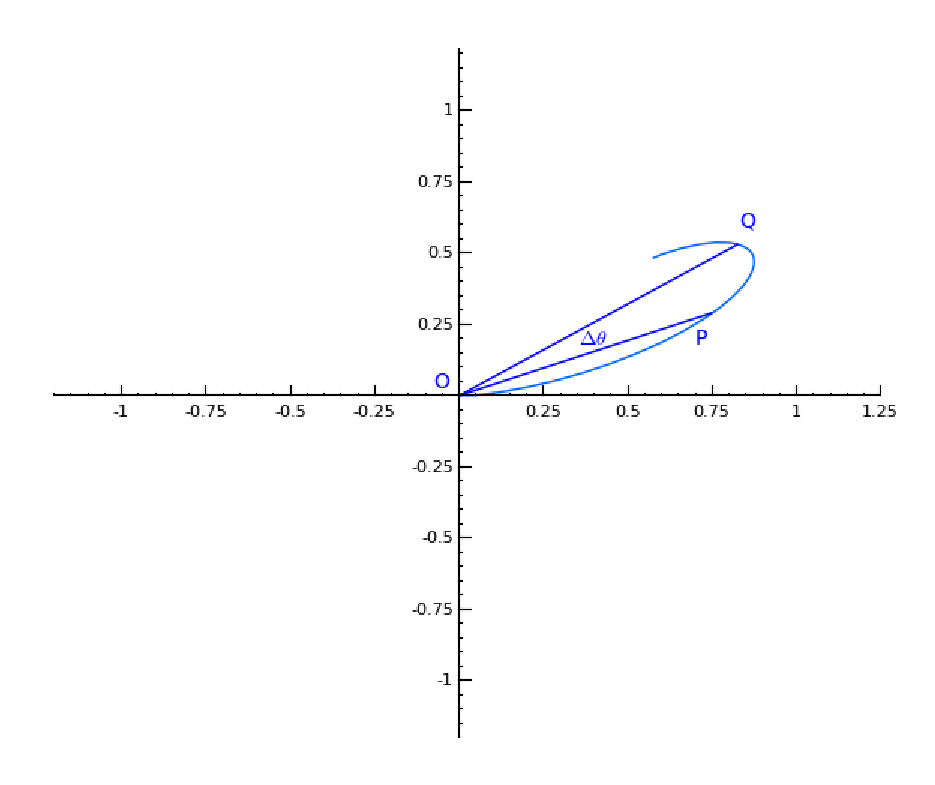
\includegraphics[height=6cm,width=9cm]{polar-tangent.eps}%
\lthtmlpictureZ
\lthtmlcheckvsize\clearpage}

{\newpage\clearpage
\lthtmlinlinemathA{tex2html_wrap_inline49388}%
$ (\rho + \Delta \rho,\theta + \Delta \theta)$%
\lthtmlinlinemathZ
\lthtmlcheckvsize\clearpage}

{\newpage\clearpage
\lthtmlinlinemathA{tex2html_wrap_inline49390}%
$ OQ = \rho + \Delta \rho$%
\lthtmlinlinemathZ
\lthtmlcheckvsize\clearpage}

{\newpage\clearpage
\lthtmlinlinemathA{tex2html_wrap_inline49392}%
$ PR = \rho \sin\Delta \theta$%
\lthtmlinlinemathZ
\lthtmlcheckvsize\clearpage}

{\newpage\clearpage
\lthtmlinlinemathA{tex2html_wrap_inline49394}%
$ OR = \rho \cos\Delta \theta$%
\lthtmlinlinemathZ
\lthtmlcheckvsize\clearpage}

{\newpage\clearpage
\lthtmlinlinemathA{tex2html_wrap_indisplay49396}%
$\displaystyle \tan PQR = \frac{PR}{RQ} 
= \frac{PR}{OQ - OR} 
= \frac{\rho \sin \Delta \theta}{\rho + \Delta \rho - \rho \cos \Delta \theta}.
$%
\lthtmlindisplaymathZ
\lthtmlcheckvsize\clearpage}

{\newpage\clearpage
\lthtmlinlinemathA{tex2html_wrap_inline49398}%
$ \psi$%
\lthtmlinlinemathZ
\lthtmlcheckvsize\clearpage}

{\newpage\clearpage
\lthtmlinlinemathA{tex2html_wrap_indisplay49410}%
$\displaystyle \tan\  \psi 	
=\  \lim_{\Delta \theta \to 0} \frac{\rho \Delta \theta}{\rho + \Delta \rho - \rho \cos \Delta \theta}
=\  \lim_{\Delta \theta \to 0} \frac{\rho \Delta \theta}{2 \rho \sin^2 \frac{\Delta \theta}{2} + \Delta \rho}
$%
\lthtmlindisplaymathZ
\lthtmlcheckvsize\clearpage}

{\newpage\clearpage
\lthtmlinlinemathA{tex2html_wrap_inline49412}%
$ \rho - \rho \cos \Delta \theta 
= \rho (1 - \cos \Delta \theta)= 2 \rho \sin^2 \frac{\Delta \theta}{2}$%
\lthtmlinlinemathZ
\lthtmlcheckvsize\clearpage}

{\newpage\clearpage
\lthtmlinlinemathA{tex2html_wrap_indisplay49416}%
$\displaystyle =\  \lim_{\Delta \theta \to 0} \frac{\frac{\rho \sin \Delta \theta}{\Delta \theta}}{\frac{2 \rho \sin^2 \frac{\Delta \theta}{2}}{\Delta \theta} + \frac{\Delta \rho}{\Delta \theta}}
=\  \lim_{\Delta \to 0} \frac{\rho \cdot \frac{\sin \Delta \theta}{\Delta \theta}}{\rho \sin \frac{\Delta \theta}{2} \cdot \frac{\sin \frac{\Delta \theta}{2}}{\frac{\Delta \theta}{2}} + \frac{\Delta \rho}{\Delta \theta}}.
$%
\lthtmlindisplaymathZ
\lthtmlcheckvsize\clearpage}

{\newpage\clearpage
\lthtmlinlinemathA{tex2html_wrap_indisplay49418}%
$\displaystyle \lim_{\Delta \theta \to 0} \left ( \frac{\Delta \rho}{\Delta \theta} \right ) 
= \frac{d\rho}{d\theta}\  {\rm and}\  \lim_{\Delta \theta \to 0} \left ( \sin \frac{\Delta \theta}{2} \right ) 
= 0,
$%
\lthtmlindisplaymathZ
\lthtmlcheckvsize\clearpage}

{\newpage\clearpage
\lthtmlinlinemathA{tex2html_wrap_indisplay49420}%
$\displaystyle \lim_{\Delta \theta \to 0} \left ( \frac{\sin \Delta \theta}{\Delta \theta} \right ) = 1
$%
\lthtmlindisplaymathZ
\lthtmlcheckvsize\clearpage}

{\newpage\clearpage
\lthtmlinlinemathA{tex2html_wrap_indisplay49422}%
$\displaystyle \lim_{\Delta \theta \to 0} \frac{\sin \frac{\Delta \theta}{2}}{\frac{\Delta \theta}{2}} = 1
$%
\lthtmlindisplaymathZ
\lthtmlcheckvsize\clearpage}

{\newpage\clearpage
\lthtmlinlinemathA{tex2html_wrap_indisplay49424}%
$\displaystyle \tan\  \psi = \frac{\rho}{\frac{d\rho}{d\theta}}$%
\lthtmlindisplaymathZ
\lthtmlcheckvsize\clearpage}

{\newpage\clearpage
\lthtmlinlinemathA{tex2html_wrap_indisplay49426}%
$\displaystyle \tau = \theta + \psi.$%
\lthtmlindisplaymathZ
\lthtmlcheckvsize\clearpage}

{\newpage\clearpage
\lthtmlinlinemathA{tex2html_wrap_inline49430}%
$ \tan\,\tau$%
\lthtmlinlinemathZ
\lthtmlcheckvsize\clearpage}

{\newpage\clearpage
\lthtmlinlinemathA{tex2html_wrap_indisplay49432}%
$\displaystyle \tan \tau = \tan (\theta + \psi) = \frac{\tan \theta + \tan \psi}{1 - \tan \theta \tan \psi}
$%
\lthtmlindisplaymathZ
\lthtmlcheckvsize\clearpage}

{\newpage\clearpage
\lthtmlinlinemathA{tex2html_wrap_inline49434}%
$ \tan\, \psi$%
\lthtmlinlinemathZ
\lthtmlcheckvsize\clearpage}

{\newpage\clearpage
\lthtmlinlinemathA{tex2html_wrap_indisplay49436}%
$\displaystyle {\rm slope\  of\  tangent}\  = \tan \tau = \frac{\tan \theta + \tan \psi}{1 - \tan \theta \tan \psi}.$%
\lthtmlindisplaymathZ
\lthtmlcheckvsize\clearpage}

{\newpage\clearpage
\lthtmlinlinemathA{tex2html_wrap_inline49447}%
$ \psi = a(1 -\cos\,\theta)$%
\lthtmlinlinemathZ
\lthtmlcheckvsize\clearpage}

{\newpage\clearpage
\lthtmlinlinemathA{tex2html_wrap_inline49449}%
$ \theta = \frac{\pi}{6}$%
\lthtmlinlinemathZ
\lthtmlcheckvsize\clearpage}

{\newpage\clearpage
\lthtmlinlinemathA{tex2html_wrap_inline49451}%
$ \frac{d\psi}{d\theta} = a \sin \theta$%
\lthtmlinlinemathZ
\lthtmlcheckvsize\clearpage}

{\newpage\clearpage
\lthtmlinlinemathA{tex2html_wrap_indisplay49453}%
$\displaystyle \tan \psi 
= \frac{\rho}{\frac{d\rho}{d\theta}} 
= \frac{a(1 - \cos \theta)}{a \sin \theta} 
= \frac{2 a \sin^2 \frac{\theta}{2}}{2a \sin \frac{\theta}{2} \cos \frac{\theta}{2}} 
= \tan \frac{\theta}{2},
$%
\lthtmlindisplaymathZ
\lthtmlcheckvsize\clearpage}

{\newpage\clearpage
\lthtmlinlinemathA{tex2html_wrap_inline49455}%
$ \tan \psi = \tan \frac{\theta}{2}$%
\lthtmlinlinemathZ
\lthtmlcheckvsize\clearpage}

{\newpage\clearpage
\lthtmlinlinemathA{tex2html_wrap_inline49457}%
$ \psi = \frac{\theta}{2}$%
\lthtmlinlinemathZ
\lthtmlcheckvsize\clearpage}

{\newpage\clearpage
\lthtmlinlinemathA{tex2html_wrap_inline49459}%
$ \tau = \theta + \frac{\theta}{2} = \frac{3\theta}{2}$%
\lthtmlinlinemathZ
\lthtmlcheckvsize\clearpage}

{\newpage\clearpage
\lthtmlinlinemathA{tex2html_wrap_indisplay49461}%
$\displaystyle \tan\, \tau = \tan \frac{\pi}{4} = 1. 
$%
\lthtmlindisplaymathZ
\lthtmlcheckvsize\clearpage}

{\newpage\clearpage
\lthtmlinlinemathA{tex2html_wrap_inline49467}%
$ C'$%
\lthtmlinlinemathZ
\lthtmlcheckvsize\clearpage}

{\newpage\clearpage
\lthtmlpictureA{tex2html_wrap49469}%
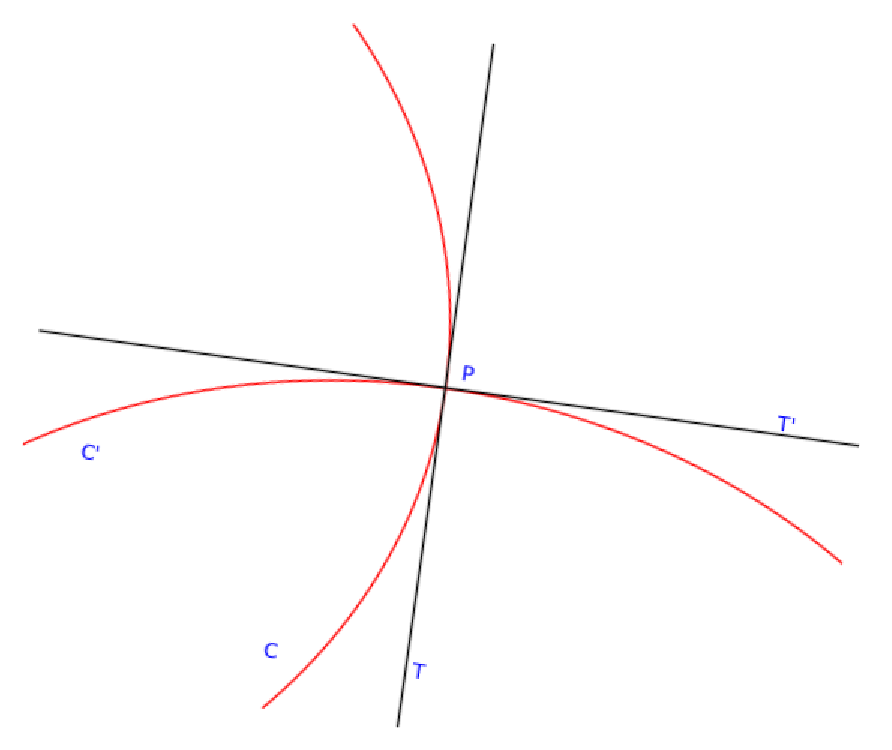
\includegraphics[height=5cm,width=8cm]{curves-intersect2.eps}%
\lthtmlpictureZ
\lthtmlcheckvsize\clearpage}

{\newpage\clearpage
\lthtmlinlinemathA{tex2html_wrap_inline49474}%
$ '$%
\lthtmlinlinemathZ
\lthtmlcheckvsize\clearpage}

{\newpage\clearpage
\lthtmlinlinemathA{tex2html_wrap_inline49478}%
$ \phi = \psi' - \psi$%
\lthtmlinlinemathZ
\lthtmlcheckvsize\clearpage}

{\newpage\clearpage
\lthtmlinlinemathA{tex2html_wrap_indisplay49480}%
$\displaystyle \  \tan\, \phi 	= \frac{\tan\, \psi' - \tan\, \psi}{1 + \tan\, \psi' \tan\, \psi},$%
\lthtmlindisplaymathZ
\lthtmlcheckvsize\clearpage}

{\newpage\clearpage
\lthtmlinlinemathA{tex2html_wrap_inline49482}%
$ \tan\, \psi'$%
\lthtmlinlinemathZ
\lthtmlcheckvsize\clearpage}

{\newpage\clearpage
\lthtmlinlinemathA{tex2html_wrap_inline49491}%
$ \rho = a\sin\, 2\theta$%
\lthtmlinlinemathZ
\lthtmlcheckvsize\clearpage}

{\newpage\clearpage
\lthtmlinlinemathA{tex2html_wrap_inline49493}%
$ \rho = a\cos\, 2\theta$%
\lthtmlinlinemathZ
\lthtmlcheckvsize\clearpage}

{\newpage\clearpage
\lthtmlinlinemathA{tex2html_wrap_indisplay49495}%
$\displaystyle \tan\, 2\theta = 1, \,\  \ \  \  2\theta = 45^o=\pi/4,\  \ \   \theta = \frac{45}{2}^o=\pi/8.
$%
\lthtmlindisplaymathZ
\lthtmlcheckvsize\clearpage}

{\newpage\clearpage
\lthtmlinlinemathA{tex2html_wrap_indisplay49497}%
$\displaystyle \tan \psi' = \frac{1}{2} \tan 2 \theta = \frac{1}{2}, 
$%
\lthtmlindisplaymathZ
\lthtmlcheckvsize\clearpage}

{\newpage\clearpage
\lthtmlinlinemathA{tex2html_wrap_inline49499}%
$ \theta = \frac{45}{2}^o=\pi/8$%
\lthtmlinlinemathZ
\lthtmlcheckvsize\clearpage}

{\newpage\clearpage
\lthtmlinlinemathA{tex2html_wrap_indisplay49501}%
$\displaystyle \tan \psi = -\frac{1}{2} \cot 2 \theta = -\frac{1}{2}, 
$%
\lthtmlindisplaymathZ
\lthtmlcheckvsize\clearpage}

{\newpage\clearpage
\lthtmlinlinemathA{tex2html_wrap_indisplay49505}%
$\displaystyle \tan \psi = \frac{ \frac{1}{2} + \frac{1}{2} }{ 1 - \frac{1}{4} } 
= \frac{4}{3}. 
$%
\lthtmlindisplaymathZ
\lthtmlcheckvsize\clearpage}

{\newpage\clearpage
\lthtmlinlinemathA{tex2html_wrap_inline49507}%
$ \psi = \arctan \frac{4}{3}$%
\lthtmlinlinemathZ
\lthtmlcheckvsize\clearpage}

\stepcounter{section}
{\newpage\clearpage
\lthtmlinlinemathA{tex2html_wrap_inline49516}%
$ \frac{d\theta}{d\rho}$%
\lthtmlinlinemathZ
\lthtmlcheckvsize\clearpage}

{\newpage\clearpage
\lthtmlpictureA{tex2html_wrap49522}%
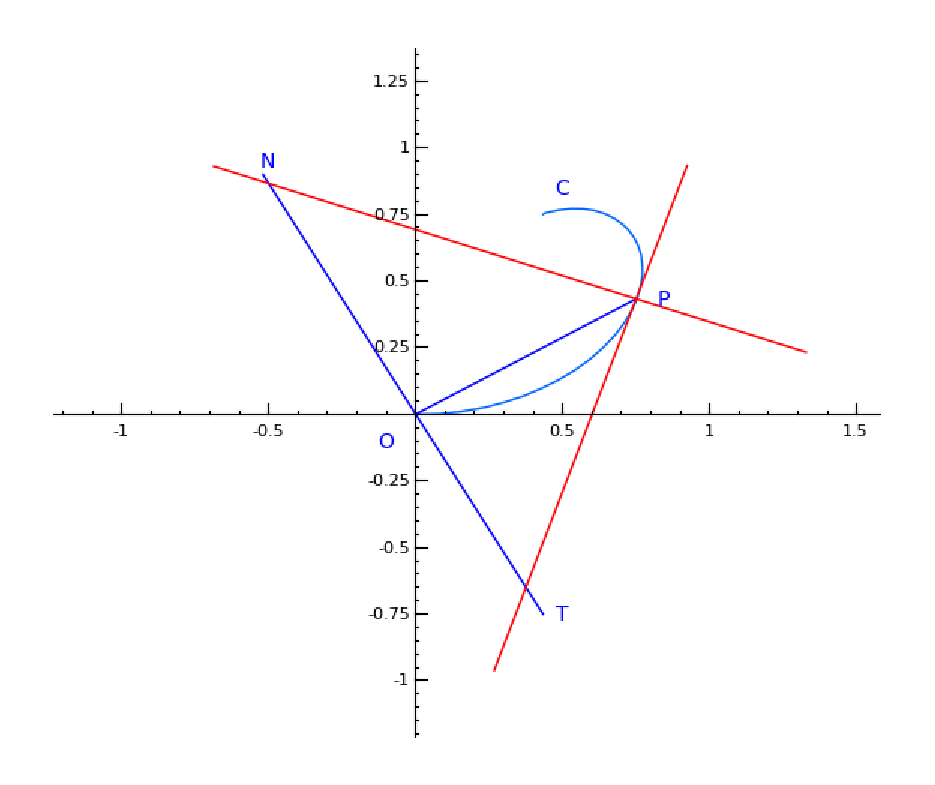
\includegraphics[height=6cm,width=6cm]{polar-subtangent2.eps}%
\lthtmlpictureZ
\lthtmlcheckvsize\clearpage}

{\newpage\clearpage
\lthtmlinlinemathA{tex2html_wrap_inline49527}%
$ \tan\, \psi = \frac{OT}{\rho}$%
\lthtmlinlinemathZ
\lthtmlcheckvsize\clearpage}

{\newpage\clearpage
\lthtmlinlinemathA{tex2html_wrap_indisplay49529}%
$\displaystyle OT = \rho \tan \psi = \rho^2 \frac{d\theta}{d\rho}  =\  {\rm length\  of\  polar\  subtangent}.$%
\lthtmlindisplaymathZ
\lthtmlcheckvsize\clearpage}

{\newpage\clearpage
\lthtmlinlinemathA{tex2html_wrap_inline49531}%
$ \tan \psi = \frac{\rho}{ON}$%
\lthtmlinlinemathZ
\lthtmlcheckvsize\clearpage}

{\newpage\clearpage
\lthtmlinlinemathA{tex2html_wrap_indisplay49533}%
$\displaystyle ON = \frac{\rho}{\tan \psi} = \frac{d\rho}{d\theta}  =\  {\rm length\  of\  polar\  subnormal}.$%
\lthtmlindisplaymathZ
\lthtmlcheckvsize\clearpage}

{\newpage\clearpage
\lthtmlinlinemathA{tex2html_wrap_inline49540}%
$ \rho^2 = a^2\cos\, 2\theta$%
\lthtmlinlinemathZ
\lthtmlcheckvsize\clearpage}

{\newpage\clearpage
\lthtmlinlinemathA{tex2html_wrap_inline49544}%
$ 2 \rho \frac{d\rho}{d\theta} 	=\  - 2 a^2 \sin 2 \theta$%
\lthtmlinlinemathZ
\lthtmlcheckvsize\clearpage}

{\newpage\clearpage
\lthtmlinlinemathA{tex2html_wrap_inline49548}%
$ - \frac{\rho^3}{a^2 \sin 2\theta}$%
\lthtmlinlinemathZ
\lthtmlcheckvsize\clearpage}

{\newpage\clearpage
\lthtmlinlinemathA{tex2html_wrap_inline49550}%
$ - \frac{a^2 \sin 2\theta}{\rho}$%
\lthtmlinlinemathZ
\lthtmlcheckvsize\clearpage}

{\newpage\clearpage
\lthtmlinlinemathA{tex2html_wrap_inline49558}%
$ \rho = \pm a \sqrt{\cos 2 \theta}$%
\lthtmlinlinemathZ
\lthtmlcheckvsize\clearpage}

{\newpage\clearpage
\lthtmlinlinemathA{tex2html_wrap_inline49560}%
$ \pm a \cot 2 \theta \sqrt{\cos 2 \theta}$%
\lthtmlinlinemathZ
\lthtmlcheckvsize\clearpage}

\stepcounter{section}
{\newpage\clearpage
\lthtmlinlinemathA{tex2html_wrap_inline49563}%
$ \rho  = r\sin\, \theta$%
\lthtmlinlinemathZ
\lthtmlcheckvsize\clearpage}

{\newpage\clearpage
\lthtmlinlinemathA{tex2html_wrap_inline49571}%
$ \psi = \theta$%
\lthtmlinlinemathZ
\lthtmlcheckvsize\clearpage}

{\newpage\clearpage
\lthtmlinlinemathA{tex2html_wrap_inline49573}%
$ \tau=2\theta$%
\lthtmlinlinemathZ
\lthtmlcheckvsize\clearpage}

{\newpage\clearpage
\lthtmlinlinemathA{tex2html_wrap_inline49575}%
$ \rho = a \sec^ \frac{\theta}{2}$%
\lthtmlinlinemathZ
\lthtmlcheckvsize\clearpage}

{\newpage\clearpage
\lthtmlinlinemathA{tex2html_wrap_inline49577}%
$ \tau + \psi = \pi$%
\lthtmlinlinemathZ
\lthtmlcheckvsize\clearpage}

{\newpage\clearpage
\lthtmlinlinemathA{tex2html_wrap_inline49581}%
$ 2\psi = \pi + 4\theta$%
\lthtmlinlinemathZ
\lthtmlcheckvsize\clearpage}

{\newpage\clearpage
\lthtmlinlinemathA{tex2html_wrap_inline49585}%
$ \rho  = e^{a\theta}$%
\lthtmlinlinemathZ
\lthtmlcheckvsize\clearpage}

{\newpage\clearpage
\lthtmlinlinemathA{tex2html_wrap_inline49587}%
$ \rho = a \sin^3 \frac{\theta}{3}$%
\lthtmlinlinemathZ
\lthtmlcheckvsize\clearpage}

{\newpage\clearpage
\lthtmlinlinemathA{tex2html_wrap_inline49589}%
$ \tau  = 4\psi$%
\lthtmlinlinemathZ
\lthtmlcheckvsize\clearpage}

{\newpage\clearpage
\lthtmlinlinemathA{tex2html_wrap_inline49595}%
$ \tan(\psi) = \tan(\theta/3)$%
\lthtmlinlinemathZ
\lthtmlcheckvsize\clearpage}

{\newpage\clearpage
\lthtmlinlinemathA{tex2html_wrap_inline49597}%
$ \theta=3\psi$%
\lthtmlinlinemathZ
\lthtmlcheckvsize\clearpage}

{\newpage\clearpage
\lthtmlinlinemathA{tex2html_wrap_inline49599}%
$ \tau=\theta+\psi=3\psi+\psi=4\psi$%
\lthtmlinlinemathZ
\lthtmlcheckvsize\clearpage}

{\newpage\clearpage
\lthtmlinlinemathA{tex2html_wrap_inline49601}%
$ \tan\, \psi = \theta$%
\lthtmlinlinemathZ
\lthtmlcheckvsize\clearpage}

{\newpage\clearpage
\lthtmlinlinemathA{tex2html_wrap_inline49603}%
$ \rho  = a\theta$%
\lthtmlinlinemathZ
\lthtmlcheckvsize\clearpage}

{\newpage\clearpage
\lthtmlinlinemathA{tex2html_wrap_inline49607}%
$ \theta = 2\pi$%
\lthtmlinlinemathZ
\lthtmlcheckvsize\clearpage}

{\newpage\clearpage
\lthtmlinlinemathA{tex2html_wrap_inline49609}%
$ 4\pi$%
\lthtmlinlinemathZ
\lthtmlcheckvsize\clearpage}

{\newpage\clearpage
\lthtmlinlinemathA{tex2html_wrap_inline49611}%
$ \psi = 80^o 57' = 1.4128...$%
\lthtmlinlinemathZ
\lthtmlcheckvsize\clearpage}

{\newpage\clearpage
\lthtmlinlinemathA{tex2html_wrap_inline49613}%
$ 85^o 27'=1.4913...$%
\lthtmlinlinemathZ
\lthtmlcheckvsize\clearpage}

{\newpage\clearpage
\lthtmlinlinemathA{tex2html_wrap_inline49615}%
$ \rho\cos\,\theta = 2a$%
\lthtmlinlinemathZ
\lthtmlcheckvsize\clearpage}

{\newpage\clearpage
\lthtmlinlinemathA{tex2html_wrap_inline49617}%
$ \rho = 5a\sin\,\theta$%
\lthtmlinlinemathZ
\lthtmlcheckvsize\clearpage}

{\newpage\clearpage
\lthtmlinlinemathA{tex2html_wrap_inline49619}%
$ \arctan \frac{3}{4}$%
\lthtmlinlinemathZ
\lthtmlcheckvsize\clearpage}

{\newpage\clearpage
\lthtmlinlinemathA{tex2html_wrap_inline49621}%
$ \rho = a \sec^2 \frac{\theta}{2}$%
\lthtmlinlinemathZ
\lthtmlcheckvsize\clearpage}

{\newpage\clearpage
\lthtmlinlinemathA{tex2html_wrap_inline49623}%
$ \rho = b \csc^2 \frac{\theta}{2}$%
\lthtmlinlinemathZ
\lthtmlcheckvsize\clearpage}

{\newpage\clearpage
\lthtmlinlinemathA{tex2html_wrap_inline49625}%
$ \rho = a\sin\,\theta$%
\lthtmlinlinemathZ
\lthtmlcheckvsize\clearpage}

{\newpage\clearpage
\lthtmlinlinemathA{tex2html_wrap_inline49629}%
$ 0^o$%
\lthtmlinlinemathZ
\lthtmlcheckvsize\clearpage}

{\newpage\clearpage
\lthtmlinlinemathA{tex2html_wrap_inline49631}%
$ \arctan 3 \sqrt{3}$%
\lthtmlinlinemathZ
\lthtmlcheckvsize\clearpage}

{\newpage\clearpage
\lthtmlinlinemathA{tex2html_wrap_inline49633}%
$ \rho = a(l - \cos,\theta)$%
\lthtmlinlinemathZ
\lthtmlcheckvsize\clearpage}

{\newpage\clearpage
\lthtmlinlinemathA{tex2html_wrap_inline49639}%
$ \rho = a\sec^2 \theta$%
\lthtmlinlinemathZ
\lthtmlcheckvsize\clearpage}

{\newpage\clearpage
\lthtmlinlinemathA{tex2html_wrap_inline49641}%
$ \rho = 2a$%
\lthtmlinlinemathZ
\lthtmlcheckvsize\clearpage}

{\newpage\clearpage
\lthtmlinlinemathA{tex2html_wrap_inline49645}%
$ \rho = a\sin\, 4\theta$%
\lthtmlinlinemathZ
\lthtmlcheckvsize\clearpage}

{\newpage\clearpage
\lthtmlinlinemathA{tex2html_wrap_inline49647}%
$ 0, 1, \infty, -1$%
\lthtmlinlinemathZ
\lthtmlcheckvsize\clearpage}

{\newpage\clearpage
\lthtmlinlinemathA{tex2html_wrap_inline49649}%
$ \rho^2 = a^2\sin\, 4\theta$%
\lthtmlinlinemathZ
\lthtmlcheckvsize\clearpage}

{\newpage\clearpage
\lthtmlinlinemathA{tex2html_wrap_inline49653}%
$ \rho = a\sin\, 3\theta$%
\lthtmlinlinemathZ
\lthtmlcheckvsize\clearpage}

{\newpage\clearpage
\lthtmlinlinemathA{tex2html_wrap_inline49655}%
$ 0, \sqrt{3}, -\sqrt{3}$%
\lthtmlinlinemathZ
\lthtmlcheckvsize\clearpage}

{\newpage\clearpage
\lthtmlinlinemathA{tex2html_wrap_inline49657}%
$ \rho = a\cos\, 3\theta$%
\lthtmlinlinemathZ
\lthtmlcheckvsize\clearpage}

{\newpage\clearpage
\lthtmlinlinemathA{tex2html_wrap_inline49663}%
$ \theta = \frac{\pi}{4}$%
\lthtmlinlinemathZ
\lthtmlcheckvsize\clearpage}

{\newpage\clearpage
\lthtmlinlinemathA{tex2html_wrap_inline49673}%
$ \rho\theta = a$%
\lthtmlinlinemathZ
\lthtmlcheckvsize\clearpage}

{\newpage\clearpage
\lthtmlinlinemathA{tex2html_wrap_inline49677}%
$ \rho = e^\theta$%
\lthtmlinlinemathZ
\lthtmlcheckvsize\clearpage}

{\newpage\clearpage
\lthtmlinlinemathA{tex2html_wrap_inline49679}%
$ \theta =  0$%
\lthtmlinlinemathZ
\lthtmlcheckvsize\clearpage}

{\newpage\clearpage
\lthtmlinlinemathA{tex2html_wrap_inline49725}%
$ \rho = \frac{a}{\theta}$%
\lthtmlinlinemathZ
\lthtmlcheckvsize\clearpage}

{\newpage\clearpage
\lthtmlinlinemathA{tex2html_wrap_inline49729}%
$ \rho\sin\, \theta = 2a$%
\lthtmlinlinemathZ
\lthtmlcheckvsize\clearpage}

{\newpage\clearpage
\lthtmlinlinemathA{tex2html_wrap_inline49733}%
$ \rho = a(1 + \cos\, \theta)$%
\lthtmlinlinemathZ
\lthtmlcheckvsize\clearpage}

{\newpage\clearpage
\lthtmlinlinemathA{tex2html_wrap_inline49735}%
$ \rho = a(1 - \cos\, \theta)$%
\lthtmlinlinemathZ
\lthtmlcheckvsize\clearpage}

{\newpage\clearpage
\lthtmlinlinemathA{tex2html_wrap_inline49739}%
$ \frac{\rho^2}{a}$%
\lthtmlinlinemathZ
\lthtmlcheckvsize\clearpage}

{\newpage\clearpage
\lthtmlinlinemathA{tex2html_wrap_inline49741}%
$ \frac{\rho}{a} \sqrt{a^2 + \rho^2}$%
\lthtmlinlinemathZ
\lthtmlcheckvsize\clearpage}

{\newpage\clearpage
\lthtmlinlinemathA{tex2html_wrap_inline49745}%
$ \sqrt{a^2 + \rho^2}$%
\lthtmlinlinemathZ
\lthtmlcheckvsize\clearpage}

{\newpage\clearpage
\lthtmlinlinemathA{tex2html_wrap_inline49747}%
$ \rho  = a^\theta$%
\lthtmlinlinemathZ
\lthtmlcheckvsize\clearpage}

{\newpage\clearpage
\lthtmlinlinemathA{tex2html_wrap_inline49749}%
$ \frac{\rho}{\log a}$%
\lthtmlinlinemathZ
\lthtmlcheckvsize\clearpage}

{\newpage\clearpage
\lthtmlinlinemathA{tex2html_wrap_inline49751}%
$ \rho \sqrt{1 + \frac{1}{\log^2 a}}$%
\lthtmlinlinemathZ
\lthtmlcheckvsize\clearpage}

{\newpage\clearpage
\lthtmlinlinemathA{tex2html_wrap_inline49753}%
$ \rho\log\, a$%
\lthtmlinlinemathZ
\lthtmlcheckvsize\clearpage}

{\newpage\clearpage
\lthtmlinlinemathA{tex2html_wrap_inline49755}%
$ \rho \sqrt{1 + \log^2 a}$%
\lthtmlinlinemathZ
\lthtmlcheckvsize\clearpage}

{\newpage\clearpage
\lthtmlinlinemathA{tex2html_wrap_inline49761}%
$ \rho = b(1 - \cos\, \theta)$%
\lthtmlinlinemathZ
\lthtmlcheckvsize\clearpage}

{\newpage\clearpage
\lthtmlinlinemathA{tex2html_wrap_inline49768}%
$ \rho^2\sin\, 2\theta=a^2$%
\lthtmlinlinemathZ
\lthtmlcheckvsize\clearpage}

{\newpage\clearpage
\lthtmlinlinemathA{tex2html_wrap_inline49770}%
$ \rho^2\cos\, 2\theta=b^2$%
\lthtmlinlinemathZ
\lthtmlcheckvsize\clearpage}

\stepcounter{section}
{\newpage\clearpage
\lthtmlinlinemathA{tex2html_wrap_indisplay49781}%
$\displaystyle x^4 - 7x^3 + 9x^2 + 27x - 54 = 0;
$%
\lthtmlindisplaymathZ
\lthtmlcheckvsize\clearpage}

{\newpage\clearpage
\lthtmlinlinemathA{tex2html_wrap_indisplay49785}%
$\displaystyle (x - 3)^3(x + 2) = 0.
$%
\lthtmlindisplaymathZ
\lthtmlcheckvsize\clearpage}

{\newpage\clearpage
\lthtmlinlinemathA{tex2html_wrap_indisplay49795}%
$\displaystyle f(x) = (x-a)^m\phi (x),$%
\lthtmlindisplaymathZ
\lthtmlcheckvsize\clearpage}

{\newpage\clearpage
\lthtmlinlinemathA{tex2html_wrap_indisplay49803}%
$\displaystyle f'(x) = (x-a)^m\phi '(x) + m\phi (x)(x - a)^{m - 1},
$%
\lthtmlindisplaymathZ
\lthtmlcheckvsize\clearpage}

{\newpage\clearpage
\lthtmlinlinemathA{tex2html_wrap_indisplay49805}%
$\displaystyle f'(x) = (x-a)^{m - 1}[(x - a)\phi '(x) + m\phi (x)].$%
\lthtmlindisplaymathZ
\lthtmlcheckvsize\clearpage}

{\newpage\clearpage
\lthtmlinlinemathA{tex2html_wrap_inline49809}%
$ (x - a)$%
\lthtmlinlinemathZ
\lthtmlcheckvsize\clearpage}

{\newpage\clearpage
\lthtmlinlinemathA{tex2html_wrap_inline49811}%
$ m - 1$%
\lthtmlinlinemathZ
\lthtmlcheckvsize\clearpage}

{\newpage\clearpage
\lthtmlinlinemathA{tex2html_wrap_inline49823}%
$ \beta$%
\lthtmlinlinemathZ
\lthtmlcheckvsize\clearpage}

{\newpage\clearpage
\lthtmlinlinemathA{tex2html_wrap_inline49827}%
$ (x -\beta)^{r - 1}$%
\lthtmlinlinemathZ
\lthtmlcheckvsize\clearpage}

{\newpage\clearpage
\lthtmlinlinemathA{tex2html_wrap_inline49831}%
$ f(x) = 0$%
\lthtmlinlinemathZ
\lthtmlcheckvsize\clearpage}

{\newpage\clearpage
\lthtmlinlinemathA{tex2html_wrap_inline49850}%
$ x^3 - 8x^2 + 13x - 6 = 0$%
\lthtmlinlinemathZ
\lthtmlcheckvsize\clearpage}

{\newpage\clearpage
\lthtmlinlinemathA{tex2html_wrap_inline49852}%
$ f(x) = x^3 - 8x^2 + 13x - 6$%
\lthtmlinlinemathZ
\lthtmlcheckvsize\clearpage}

{\newpage\clearpage
\lthtmlinlinemathA{tex2html_wrap_inline49854}%
$ f'(x) 	= 3x^2 - 16x + 13$%
\lthtmlinlinemathZ
\lthtmlcheckvsize\clearpage}

{\newpage\clearpage
\lthtmlinlinemathA{tex2html_wrap_inline49858}%
$ x - 1 = 0$%
\lthtmlinlinemathZ
\lthtmlcheckvsize\clearpage}

{\newpage\clearpage
\lthtmlinlinemathA{tex2html_wrap_inline49862}%
$ (x - 1)^2$%
\lthtmlinlinemathZ
\lthtmlcheckvsize\clearpage}

{\newpage\clearpage
\lthtmlinlinemathA{tex2html_wrap_inline49864}%
$ x^3 - 8x^2 + 13x - 6$%
\lthtmlinlinemathZ
\lthtmlcheckvsize\clearpage}

{\newpage\clearpage
\lthtmlinlinemathA{tex2html_wrap_inline49868}%
$ (x - 6)$%
\lthtmlinlinemathZ
\lthtmlcheckvsize\clearpage}

{\newpage\clearpage
\lthtmlpictureA{tex2html_wrap49886}%
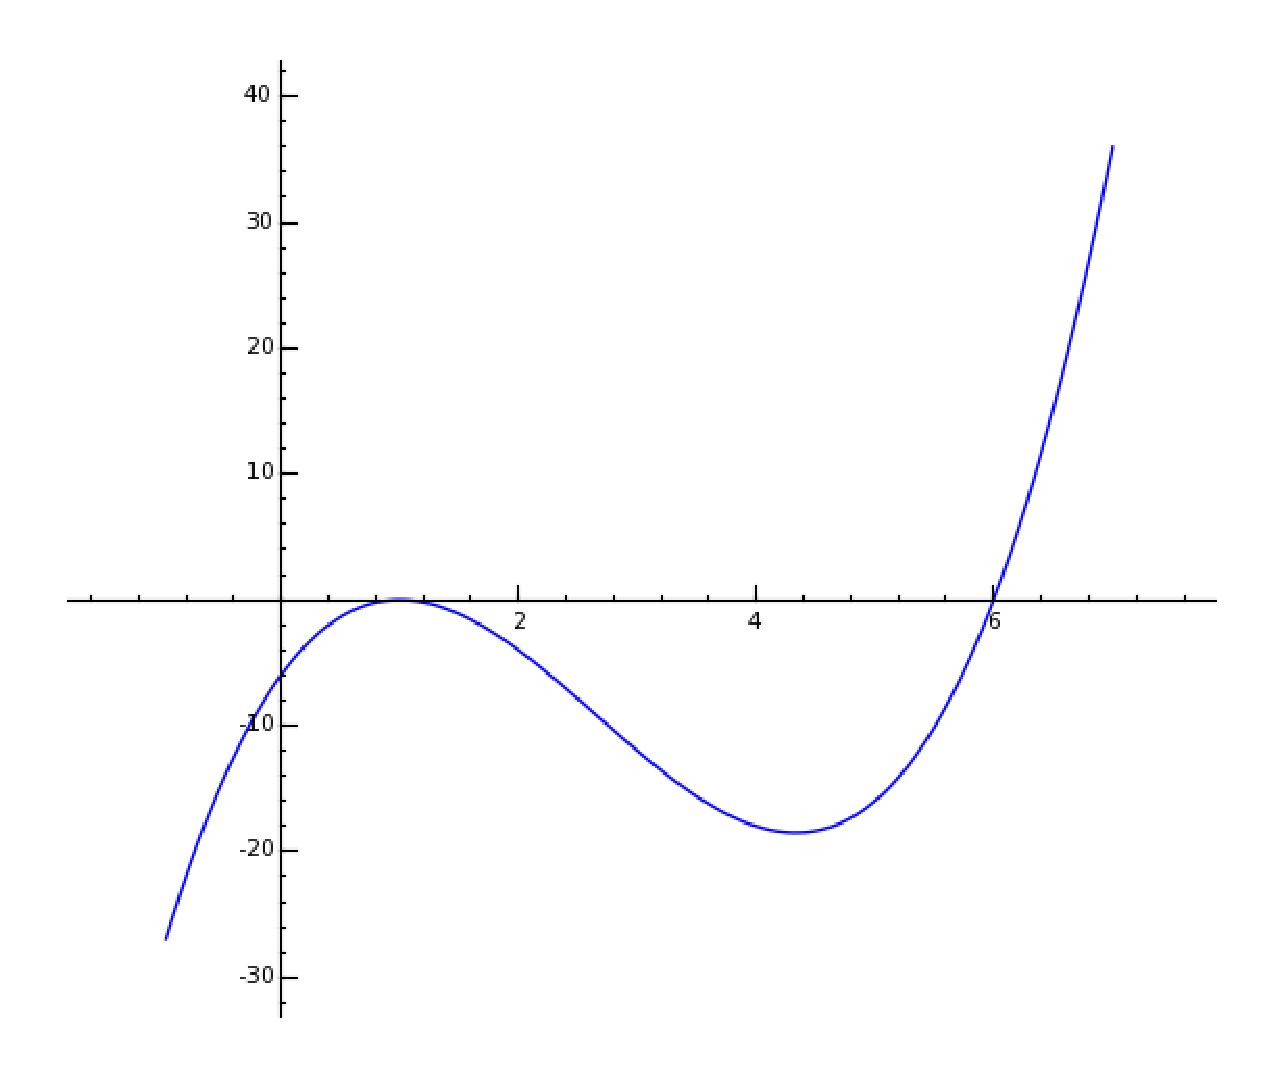
\includegraphics[height=2.5cm,width=3.5cm]{multiple-roots.eps}%
\lthtmlpictureZ
\lthtmlcheckvsize\clearpage}

\stepcounter{section}
{\newpage\clearpage
\lthtmlinlinemathA{tex2html_wrap_inline49896}%
$ x^3 - 7x^2 + 16x - 12 = 0$%
\lthtmlinlinemathZ
\lthtmlcheckvsize\clearpage}

{\newpage\clearpage
\lthtmlinlinemathA{tex2html_wrap_inline49904}%
$ x^4 - 6x^2 - 8x - 3 = 0$%
\lthtmlinlinemathZ
\lthtmlcheckvsize\clearpage}

{\newpage\clearpage
\lthtmlinlinemathA{tex2html_wrap_inline49906}%
$ x^4 - 7x^3 + 9x^2 + 27x - 64 = 0$%
\lthtmlinlinemathZ
\lthtmlcheckvsize\clearpage}

{\newpage\clearpage
\lthtmlinlinemathA{tex2html_wrap_inline49916}%
$ x^4 - 5x^3 - 9x^2 + 81x - 108 = 0$%
\lthtmlinlinemathZ
\lthtmlcheckvsize\clearpage}

{\newpage\clearpage
\lthtmlinlinemathA{tex2html_wrap_inline49924}%
$ -4$%
\lthtmlinlinemathZ
\lthtmlcheckvsize\clearpage}

{\newpage\clearpage
\lthtmlinlinemathA{tex2html_wrap_inline49926}%
$ x^4 + 6x^3 + x^2 - 24x + 16 = 0$%
\lthtmlinlinemathZ
\lthtmlcheckvsize\clearpage}

{\newpage\clearpage
\lthtmlinlinemathA{tex2html_wrap_inline49936}%
$ x^4 - 9x^3 + 23x^2 - 3x - 36 = 0$%
\lthtmlinlinemathZ
\lthtmlcheckvsize\clearpage}

{\newpage\clearpage
\lthtmlinlinemathA{tex2html_wrap_inline49946}%
$ x^4 - 6x^3 + 10x^2 - 8 = 0$%
\lthtmlinlinemathZ
\lthtmlcheckvsize\clearpage}

{\newpage\clearpage
\lthtmlinlinemathA{tex2html_wrap_inline49952}%
$ 1 \pm \sqrt{3}$%
\lthtmlinlinemathZ
\lthtmlcheckvsize\clearpage}

{\newpage\clearpage
\lthtmlinlinemathA{tex2html_wrap_inline49958}%
$ x^5 - x^4 - 5x^3 + x^2 + 8x + 4 = 0$%
\lthtmlinlinemathZ
\lthtmlcheckvsize\clearpage}

{\newpage\clearpage
\lthtmlinlinemathA{tex2html_wrap_inline49968}%
$ x^5 - 15x^3 + 10x^2 + 60x - 72 = 0$%
\lthtmlinlinemathZ
\lthtmlcheckvsize\clearpage}

{\newpage\clearpage
\lthtmlinlinemathA{tex2html_wrap_inline49980}%
$ x^5 - 3x^4 - 5x^3 + 13x^2 + 24x + l0 = 0$%
\lthtmlinlinemathZ
\lthtmlcheckvsize\clearpage}

\addtocounter{enumi}{10}
{\newpage\clearpage
\lthtmlinlinemathA{tex2html_wrap_inline49982}%
$ x^3 + 9x^2 + 2x - 48 = 0$%
\lthtmlinlinemathZ
\lthtmlcheckvsize\clearpage}

{\newpage\clearpage
\lthtmlinlinemathA{tex2html_wrap_inline49984}%
$ x^4 - 15x^2 - 10x + 24 = 0$%
\lthtmlinlinemathZ
\lthtmlcheckvsize\clearpage}

{\newpage\clearpage
\lthtmlinlinemathA{tex2html_wrap_inline49986}%
$ x^4 - 3x^3 - 6x^2 + 14x + 12 = 0$%
\lthtmlinlinemathZ
\lthtmlcheckvsize\clearpage}

{\newpage\clearpage
\lthtmlinlinemathA{tex2html_wrap_inline49988}%
$ x^n - a^n = 0$%
\lthtmlinlinemathZ
\lthtmlcheckvsize\clearpage}

{\newpage\clearpage
\lthtmlinlinemathA{tex2html_wrap_indisplay49990}%
$\displaystyle x^3 + 3qx + r = 0
$%
\lthtmlindisplaymathZ
\lthtmlcheckvsize\clearpage}

{\newpage\clearpage
\lthtmlinlinemathA{tex2html_wrap_inline49992}%
$ 4q^3 + r^2 = 0$%
\lthtmlinlinemathZ
\lthtmlcheckvsize\clearpage}

{\newpage\clearpage
\lthtmlinlinemathA{tex2html_wrap_indisplay49994}%
$\displaystyle x^3 + 3px^2 + r = 0
$%
\lthtmlindisplaymathZ
\lthtmlcheckvsize\clearpage}

{\newpage\clearpage
\lthtmlinlinemathA{tex2html_wrap_inline49996}%
$ r(4p^3 + r) = 0$%
\lthtmlinlinemathZ
\lthtmlcheckvsize\clearpage}

\stepcounter{section}
{\newpage\clearpage
\lthtmlpictureA{tex2html_wrap49999}%
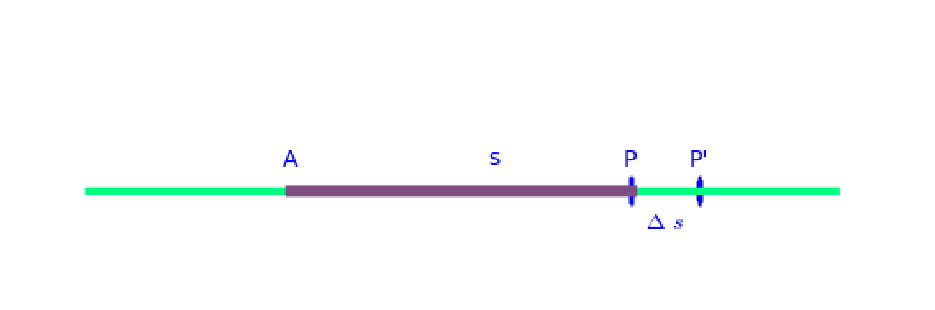
\includegraphics[height=2cm,width=8cm]{linear-motion2.eps}%
\lthtmlpictureZ
\lthtmlcheckvsize\clearpage}

{\newpage\clearpage
\lthtmlinlinemathA{tex2html_wrap_indisplay50016}%
$\displaystyle s = f(t)
$%
\lthtmlindisplaymathZ
\lthtmlcheckvsize\clearpage}

{\newpage\clearpage
\lthtmlinlinemathA{tex2html_wrap_inline50020}%
$ \Delta t$%
\lthtmlinlinemathZ
\lthtmlcheckvsize\clearpage}

{\newpage\clearpage
\lthtmlinlinemathA{tex2html_wrap_inline50028}%
$ \Delta s$%
\lthtmlinlinemathZ
\lthtmlcheckvsize\clearpage}

{\newpage\clearpage
\lthtmlinlinemathA{tex2html_wrap_indisplay50030}%
$\displaystyle \frac{\Delta s}{\Delta t} = {\rm the\  average\  velocity}$%
\lthtmlindisplaymathZ
\lthtmlcheckvsize\clearpage}

{\newpage\clearpage
\lthtmlinlinemathA{tex2html_wrap_inline50034}%
$ \frac{\Delta s}{\Delta t}$%
\lthtmlinlinemathZ
\lthtmlcheckvsize\clearpage}

{\newpage\clearpage
\lthtmlinlinemathA{tex2html_wrap_indisplay50038}%
$\displaystyle v = \lim_{\Delta t \to 0} \frac{\Delta s}{\Delta t},
$%
\lthtmlindisplaymathZ
\lthtmlcheckvsize\clearpage}

{\newpage\clearpage
\lthtmlinlinemathA{tex2html_wrap_indisplay50040}%
$\displaystyle v = \frac{ds}{dt}$%
\lthtmlindisplaymathZ
\lthtmlcheckvsize\clearpage}

{\newpage\clearpage
\lthtmlinlinemathA{tex2html_wrap_indisplay50042}%
$\displaystyle s = 16.1t^2$%
\lthtmlindisplaymathZ
\lthtmlcheckvsize\clearpage}

{\newpage\clearpage
\lthtmlinlinemathA{tex2html_wrap_inline50048}%
$ s + \Delta s = 16.1(t + \Delta t)^2 
= 16.1 t^2 + 32.2 t \cdot \Delta t + 16.1(\Delta t)^2$%
\lthtmlinlinemathZ
\lthtmlcheckvsize\clearpage}

{\newpage\clearpage
\lthtmlinlinemathA{tex2html_wrap_inline50050}%
$ \Delta s 	= 32.2t \cdot \Delta t + 16.1(\Delta t)^2$%
\lthtmlinlinemathZ
\lthtmlcheckvsize\clearpage}

{\newpage\clearpage
\lthtmlinlinemathA{tex2html_wrap_inline50052}%
$ \frac{\Delta s}{\Delta t}
= 32.2t + 16.1\Delta t = $%
\lthtmlinlinemathZ
\lthtmlcheckvsize\clearpage}

{\newpage\clearpage
\lthtmlinlinemathA{tex2html_wrap_indisplay50058}%
$\displaystyle \frac{\Delta s}{\Delta t} 	= 64.4 + 16.1\Delta t$%
\lthtmlindisplaymathZ
\lthtmlcheckvsize\clearpage}

{\newpage\clearpage
\lthtmlinlinemathA{tex2html_wrap_inline50064}%
$ \frac{1}{100}$%
\lthtmlinlinemathZ
\lthtmlcheckvsize\clearpage}

{\newpage\clearpage
\lthtmlinlinemathA{tex2html_wrap_inline50066}%
$ \frac{1}{1000}$%
\lthtmlinlinemathZ
\lthtmlcheckvsize\clearpage}

{\newpage\clearpage
\lthtmlinlinemathA{tex2html_wrap_inline50070}%
$ 64.4$%
\lthtmlinlinemathZ
\lthtmlcheckvsize\clearpage}

{\newpage\clearpage
\lthtmlinlinemathA{tex2html_wrap_indisplay50072}%
$\displaystyle v = \lim_{\Delta t \to 0} \left ( \frac{\Delta s}{\Delta t} \right ) = 64.4 \  ft./sec.
$%
\lthtmlindisplaymathZ
\lthtmlcheckvsize\clearpage}

{\newpage\clearpage
\lthtmlinlinemathA{tex2html_wrap_inline50074}%
$ 16.1 \Delta t$%
\lthtmlinlinemathZ
\lthtmlcheckvsize\clearpage}

{\newpage\clearpage
\lthtmlinlinemathA{tex2html_wrap_inline50076}%
$ 64.4 + 16.1\Delta t$%
\lthtmlinlinemathZ
\lthtmlcheckvsize\clearpage}

\stepcounter{section}
{\newpage\clearpage
\lthtmlinlinemathA{tex2html_wrap_inline50087}%
$ xy$%
\lthtmlinlinemathZ
\lthtmlcheckvsize\clearpage}

{\newpage\clearpage
\lthtmlinlinemathA{tex2html_wrap_inline50093}%
$ x = f(t)$%
\lthtmlinlinemathZ
\lthtmlcheckvsize\clearpage}

{\newpage\clearpage
\lthtmlinlinemathA{tex2html_wrap_inline50095}%
$ y = g(t)$%
\lthtmlinlinemathZ
\lthtmlcheckvsize\clearpage}

{\newpage\clearpage
\lthtmlpictureA{tex2html_wrap50097}%
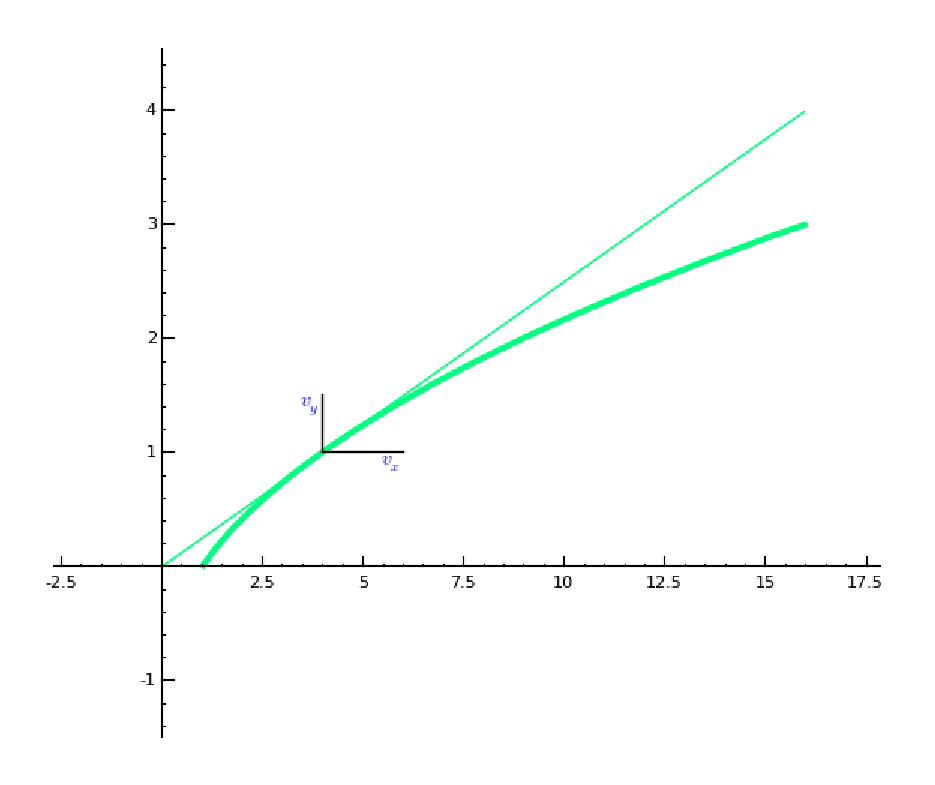
\includegraphics[height=5cm,width=8cm]{vel-comps2.eps}%
\lthtmlpictureZ
\lthtmlcheckvsize\clearpage}

{\newpage\clearpage
\lthtmlinlinemathA{tex2html_wrap_inline50106}%
$ v_x$%
\lthtmlinlinemathZ
\lthtmlcheckvsize\clearpage}

{\newpage\clearpage
\lthtmlinlinemathA{tex2html_wrap_indisplay50118}%
$\displaystyle v_x = \frac{dx}{dt}.$%
\lthtmlindisplaymathZ
\lthtmlcheckvsize\clearpage}

{\newpage\clearpage
\lthtmlinlinemathA{tex2html_wrap_indisplay50122}%
$\displaystyle v_y = \frac{dy}{dt}.$%
\lthtmlindisplaymathZ
\lthtmlcheckvsize\clearpage}

{\newpage\clearpage
\lthtmlinlinemathA{tex2html_wrap_indisplay50124}%
$\displaystyle v^2 = {v_x}^2 + {v_y}^2,
$%
\lthtmlindisplaymathZ
\lthtmlcheckvsize\clearpage}

{\newpage\clearpage
\lthtmlinlinemathA{tex2html_wrap_indisplay50126}%
$\displaystyle v = \frac{ds}{dt}  = \sqrt{\left ( \frac{dx}{dt} \right )^2 + \left ( \frac{dy}{dt} \right )^2},$%
\lthtmlindisplaymathZ
\lthtmlcheckvsize\clearpage}

{\newpage\clearpage
\lthtmlinlinemathA{tex2html_wrap_indisplay50132}%
$\displaystyle \sin \tau = \frac{v_y}{v}  = \frac{\frac{dy}{dt}}{\frac{ds}{dt}}; \  \  \cos \tau = \frac{v_x}{v} = \frac{\frac{dx}{dt}}{\frac{ds}{ds}};  \  \ \tan \tau = \frac{v_y}{v_x} = \frac{\frac{dy}{dt}}{\frac{dx}{dt}}.$%
\lthtmlindisplaymathZ
\lthtmlcheckvsize\clearpage}

\stepcounter{section}
{\newpage\clearpage
\lthtmlinlinemathA{tex2html_wrap_inline50147}%
$ \frac{\Delta v}{\Delta t}$%
\lthtmlinlinemathZ
\lthtmlcheckvsize\clearpage}

{\newpage\clearpage
\lthtmlinlinemathA{tex2html_wrap_indisplay50157}%
$\displaystyle a = \lim_{\Delta t \to 0} \left ( \frac{\Delta v}{\Delta t} \right ),
$%
\lthtmlindisplaymathZ
\lthtmlcheckvsize\clearpage}

{\newpage\clearpage
\lthtmlinlinemathA{tex2html_wrap_indisplay50159}%
$\displaystyle a = \frac{dv}{dt}$%
\lthtmlindisplaymathZ
\lthtmlcheckvsize\clearpage}

\stepcounter{section}
{\newpage\clearpage
\lthtmlinlinemathA{tex2html_wrap_inline50162}%
$ a_t$%
\lthtmlinlinemathZ
\lthtmlcheckvsize\clearpage}

{\newpage\clearpage
\lthtmlinlinemathA{tex2html_wrap_inline50164}%
$ a_n$%
\lthtmlinlinemathZ
\lthtmlcheckvsize\clearpage}

{\newpage\clearpage
\lthtmlinlinemathA{tex2html_wrap_indisplay50166}%
$\displaystyle a_t = \frac{dv}{dt};\  \ \   a_n = \frac{v^2}{R}.$%
\lthtmlindisplaymathZ
\lthtmlcheckvsize\clearpage}

{\newpage\clearpage
\lthtmlinlinemathA{tex2html_wrap_inline50168}%
$ R$%
\lthtmlinlinemathZ
\lthtmlcheckvsize\clearpage}

{\newpage\clearpage
\lthtmlinlinemathA{tex2html_wrap_indisplay50174}%
$\displaystyle a_x = \frac{dv_x}{dt}; \  \ \  \ a_y = \frac{dv_y}{dt}.$%
\lthtmlindisplaymathZ
\lthtmlcheckvsize\clearpage}

{\newpage\clearpage
\lthtmlinlinemathA{tex2html_wrap_indisplay50176}%
$\displaystyle a = \sqrt{\left ( \frac{dv_x}{dt} \right )^2 + \left ( \frac{dv_y}{dt} \right )^2},$%
\lthtmlindisplaymathZ
\lthtmlcheckvsize\clearpage}

\stepcounter{section}
{\newpage\clearpage
\lthtmlinlinemathA{tex2html_wrap_inline50222}%
$ s = 16.1t^2$%
\lthtmlinlinemathZ
\lthtmlcheckvsize\clearpage}

{\newpage\clearpage
\lthtmlinlinemathA{tex2html_wrap_inline50236}%
$ \frac{ds}{dt} = 32.2 t$%
\lthtmlinlinemathZ
\lthtmlcheckvsize\clearpage}

{\newpage\clearpage
\lthtmlinlinemathA{tex2html_wrap_inline50238}%
$ v = 32.2t$%
\lthtmlinlinemathZ
\lthtmlcheckvsize\clearpage}

{\newpage\clearpage
\lthtmlinlinemathA{tex2html_wrap_inline50240}%
$ \frac{dv}{dt} = 32.2$%
\lthtmlinlinemathZ
\lthtmlcheckvsize\clearpage}

{\newpage\clearpage
\lthtmlinlinemathA{tex2html_wrap_inline50242}%
$ a = 32.2\   \fps2$%
\lthtmlinlinemathZ
\lthtmlcheckvsize\clearpage}

{\newpage\clearpage
\lthtmlinlinemathA{tex2html_wrap_inline50244}%
$ 32.2$%
\lthtmlinlinemathZ
\lthtmlcheckvsize\clearpage}

{\newpage\clearpage
\lthtmlinlinemathA{tex2html_wrap_inline50252}%
$ v = 32.2$%
\lthtmlinlinemathZ
\lthtmlcheckvsize\clearpage}

{\newpage\clearpage
\lthtmlinlinemathA{tex2html_wrap_inline50260}%
$ t = 5$%
\lthtmlinlinemathZ
\lthtmlcheckvsize\clearpage}

{\newpage\clearpage
\lthtmlinlinemathA{tex2html_wrap_inline50262}%
$ v = 161$%
\lthtmlinlinemathZ
\lthtmlcheckvsize\clearpage}

{\newpage\clearpage
\lthtmlinlinemathA{tex2html_wrap_indisplay50266}%
$\displaystyle x = v_0 \cos \phi \cdot t,\  \ \   y = v_0 \sin \phi \cdot t - 16.1 t^2;
$%
\lthtmlindisplaymathZ
\lthtmlcheckvsize\clearpage}

{\newpage\clearpage
\lthtmlinlinemathA{tex2html_wrap_inline50268}%
$ v_0$%
\lthtmlinlinemathZ
\lthtmlcheckvsize\clearpage}

{\newpage\clearpage
\lthtmlinlinemathA{tex2html_wrap_inline50281}%
$ v_0 = 100$%
\lthtmlinlinemathZ
\lthtmlcheckvsize\clearpage}

{\newpage\clearpage
\lthtmlinlinemathA{tex2html_wrap_inline50283}%
$ \phi = 30^0 = \pi/6$%
\lthtmlinlinemathZ
\lthtmlcheckvsize\clearpage}

{\newpage\clearpage
\lthtmlinlinemathA{tex2html_wrap_inline50288}%
$ v_x = v_0 \cos \phi$%
\lthtmlinlinemathZ
\lthtmlcheckvsize\clearpage}

{\newpage\clearpage
\lthtmlinlinemathA{tex2html_wrap_inline50290}%
$ v_y = v_0 \sin \phi - 32.2 t$%
\lthtmlinlinemathZ
\lthtmlcheckvsize\clearpage}

{\newpage\clearpage
\lthtmlinlinemathA{tex2html_wrap_inline50292}%
$ v = \sqrt{{v_0}^2 - 64.4 t v_0 \sin \phi + 1036.8 t^2}$%
\lthtmlinlinemathZ
\lthtmlcheckvsize\clearpage}

{\newpage\clearpage
\lthtmlinlinemathA{tex2html_wrap_inline50294}%
$ a_x = 0$%
\lthtmlinlinemathZ
\lthtmlcheckvsize\clearpage}

{\newpage\clearpage
\lthtmlinlinemathA{tex2html_wrap_inline50296}%
$ a_y = − 32.2$%
\lthtmlinlinemathZ
\lthtmlcheckvsize\clearpage}

{\newpage\clearpage
\lthtmlinlinemathA{tex2html_wrap_inline50298}%
$ a =  32.2$%
\lthtmlinlinemathZ
\lthtmlcheckvsize\clearpage}

{\newpage\clearpage
\lthtmlinlinemathA{tex2html_wrap_inline50306}%
$ v_x = 86.6$%
\lthtmlinlinemathZ
\lthtmlcheckvsize\clearpage}

{\newpage\clearpage
\lthtmlinlinemathA{tex2html_wrap_inline50310}%
$ v_y = 17.8$%
\lthtmlinlinemathZ
\lthtmlcheckvsize\clearpage}

{\newpage\clearpage
\lthtmlinlinemathA{tex2html_wrap_inline50312}%
$ a_y = - 32.2\  \fps2$%
\lthtmlinlinemathZ
\lthtmlcheckvsize\clearpage}

{\newpage\clearpage
\lthtmlinlinemathA{tex2html_wrap_inline50314}%
$ v = 88.4$%
\lthtmlinlinemathZ
\lthtmlcheckvsize\clearpage}

{\newpage\clearpage
\lthtmlinlinemathA{tex2html_wrap_inline50318}%
$ \tau = \arctan \frac{v_y}{v_x} = \arctan \frac{17.8}{86.6} = 0.2027...
\approx 11^o$%
\lthtmlinlinemathZ
\lthtmlcheckvsize\clearpage}

{\newpage\clearpage
\lthtmlinlinemathA{tex2html_wrap_inline50336}%
$ s = t^3 + 2t^2$%
\lthtmlinlinemathZ
\lthtmlcheckvsize\clearpage}

{\newpage\clearpage
\lthtmlinlinemathA{tex2html_wrap_inline50340}%
$ s = 16$%
\lthtmlinlinemathZ
\lthtmlcheckvsize\clearpage}

{\newpage\clearpage
\lthtmlinlinemathA{tex2html_wrap_inline50342}%
$ v = 20$%
\lthtmlinlinemathZ
\lthtmlcheckvsize\clearpage}

{\newpage\clearpage
\lthtmlinlinemathA{tex2html_wrap_inline50344}%
$ a = 16$%
\lthtmlinlinemathZ
\lthtmlcheckvsize\clearpage}

{\newpage\clearpage
\lthtmlinlinemathA{tex2html_wrap_inline50346}%
$ s = t^2 + 2t$%
\lthtmlinlinemathZ
\lthtmlcheckvsize\clearpage}

{\newpage\clearpage
\lthtmlinlinemathA{tex2html_wrap_inline50350}%
$ s = 15$%
\lthtmlinlinemathZ
\lthtmlcheckvsize\clearpage}

{\newpage\clearpage
\lthtmlinlinemathA{tex2html_wrap_inline50352}%
$ v = 8$%
\lthtmlinlinemathZ
\lthtmlcheckvsize\clearpage}

{\newpage\clearpage
\lthtmlinlinemathA{tex2html_wrap_inline50354}%
$ a = 2$%
\lthtmlinlinemathZ
\lthtmlcheckvsize\clearpage}

{\newpage\clearpage
\lthtmlinlinemathA{tex2html_wrap_inline50356}%
$ s = 3 - 4t$%
\lthtmlinlinemathZ
\lthtmlcheckvsize\clearpage}

{\newpage\clearpage
\lthtmlinlinemathA{tex2html_wrap_inline50358}%
$ t = 4$%
\lthtmlinlinemathZ
\lthtmlcheckvsize\clearpage}

{\newpage\clearpage
\lthtmlinlinemathA{tex2html_wrap_inline50360}%
$ s = - 13$%
\lthtmlinlinemathZ
\lthtmlcheckvsize\clearpage}

{\newpage\clearpage
\lthtmlinlinemathA{tex2html_wrap_inline50362}%
$ v = - 4$%
\lthtmlinlinemathZ
\lthtmlcheckvsize\clearpage}

{\newpage\clearpage
\lthtmlinlinemathA{tex2html_wrap_inline50364}%
$ a = 0$%
\lthtmlinlinemathZ
\lthtmlcheckvsize\clearpage}

{\newpage\clearpage
\lthtmlinlinemathA{tex2html_wrap_inline50366}%
$ x = 2t - t^2$%
\lthtmlinlinemathZ
\lthtmlcheckvsize\clearpage}

{\newpage\clearpage
\lthtmlinlinemathA{tex2html_wrap_inline50372}%
$ v = 0$%
\lthtmlinlinemathZ
\lthtmlcheckvsize\clearpage}

{\newpage\clearpage
\lthtmlinlinemathA{tex2html_wrap_inline50374}%
$ a = - 2$%
\lthtmlinlinemathZ
\lthtmlcheckvsize\clearpage}

{\newpage\clearpage
\lthtmlinlinemathA{tex2html_wrap_inline50376}%
$ y = 2t - t^3$%
\lthtmlinlinemathZ
\lthtmlcheckvsize\clearpage}

{\newpage\clearpage
\lthtmlinlinemathA{tex2html_wrap_inline50380}%
$ y = 0$%
\lthtmlinlinemathZ
\lthtmlcheckvsize\clearpage}

{\newpage\clearpage
\lthtmlinlinemathA{tex2html_wrap_inline50382}%
$ v = 2$%
\lthtmlinlinemathZ
\lthtmlcheckvsize\clearpage}

{\newpage\clearpage
\lthtmlinlinemathA{tex2html_wrap_inline50386}%
$ h = 20t + 16t^2$%
\lthtmlinlinemathZ
\lthtmlcheckvsize\clearpage}

{\newpage\clearpage
\lthtmlinlinemathA{tex2html_wrap_inline50388}%
$ t = 10$%
\lthtmlinlinemathZ
\lthtmlcheckvsize\clearpage}

{\newpage\clearpage
\lthtmlinlinemathA{tex2html_wrap_inline50390}%
$ h = 1800$%
\lthtmlinlinemathZ
\lthtmlcheckvsize\clearpage}

{\newpage\clearpage
\lthtmlinlinemathA{tex2html_wrap_inline50392}%
$ v = 340$%
\lthtmlinlinemathZ
\lthtmlcheckvsize\clearpage}

{\newpage\clearpage
\lthtmlinlinemathA{tex2html_wrap_inline50394}%
$ a = 32$%
\lthtmlinlinemathZ
\lthtmlcheckvsize\clearpage}

{\newpage\clearpage
\lthtmlinlinemathA{tex2html_wrap_inline50396}%
$ s = 2 \sin\, t$%
\lthtmlinlinemathZ
\lthtmlcheckvsize\clearpage}

{\newpage\clearpage
\lthtmlinlinemathA{tex2html_wrap_inline50400}%
$ s = \sqrt{2}$%
\lthtmlinlinemathZ
\lthtmlcheckvsize\clearpage}

{\newpage\clearpage
\lthtmlinlinemathA{tex2html_wrap_inline50402}%
$ v = \sqrt{2}$%
\lthtmlinlinemathZ
\lthtmlcheckvsize\clearpage}

{\newpage\clearpage
\lthtmlinlinemathA{tex2html_wrap_inline50404}%
$ a= - \sqrt{2}$%
\lthtmlinlinemathZ
\lthtmlcheckvsize\clearpage}

{\newpage\clearpage
\lthtmlinlinemathA{tex2html_wrap_inline50406}%
$ y = a \cos \frac{\pi t}{3}$%
\lthtmlinlinemathZ
\lthtmlcheckvsize\clearpage}

{\newpage\clearpage
\lthtmlinlinemathA{tex2html_wrap_inline50410}%
$ y = \frac{a}{2}$%
\lthtmlinlinemathZ
\lthtmlcheckvsize\clearpage}

{\newpage\clearpage
\lthtmlinlinemathA{tex2html_wrap_inline50412}%
$ v = -\frac{\pi a \sqrt{3}}{6}$%
\lthtmlinlinemathZ
\lthtmlcheckvsize\clearpage}

{\newpage\clearpage
\lthtmlinlinemathA{tex2html_wrap_inline50414}%
$ a = -\frac{\pi^2 a}{18}$%
\lthtmlinlinemathZ
\lthtmlcheckvsize\clearpage}

{\newpage\clearpage
\lthtmlinlinemathA{tex2html_wrap_inline50416}%
$ s = 2e^{3t}$%
\lthtmlinlinemathZ
\lthtmlcheckvsize\clearpage}

{\newpage\clearpage
\lthtmlinlinemathA{tex2html_wrap_inline50420}%
$ s = 2$%
\lthtmlinlinemathZ
\lthtmlcheckvsize\clearpage}

{\newpage\clearpage
\lthtmlinlinemathA{tex2html_wrap_inline50422}%
$ v = 6$%
\lthtmlinlinemathZ
\lthtmlcheckvsize\clearpage}

{\newpage\clearpage
\lthtmlinlinemathA{tex2html_wrap_inline50424}%
$ a = 18$%
\lthtmlinlinemathZ
\lthtmlcheckvsize\clearpage}

{\newpage\clearpage
\lthtmlinlinemathA{tex2html_wrap_inline50426}%
$ s = 2t^2 - 3t$%
\lthtmlinlinemathZ
\lthtmlcheckvsize\clearpage}

{\newpage\clearpage
\lthtmlinlinemathA{tex2html_wrap_inline50430}%
$ x = 4 + t^3$%
\lthtmlinlinemathZ
\lthtmlcheckvsize\clearpage}

{\newpage\clearpage
\lthtmlinlinemathA{tex2html_wrap_inline50434}%
$ y = 5 \cos\, 2t$%
\lthtmlinlinemathZ
\lthtmlcheckvsize\clearpage}

{\newpage\clearpage
\lthtmlinlinemathA{tex2html_wrap_inline50438}%
$ s = b \sin \frac{\pi t}{4}$%
\lthtmlinlinemathZ
\lthtmlcheckvsize\clearpage}

{\newpage\clearpage
\lthtmlinlinemathA{tex2html_wrap_inline50442}%
$ x = ae^{- 2t}$%
\lthtmlinlinemathZ
\lthtmlcheckvsize\clearpage}

{\newpage\clearpage
\lthtmlinlinemathA{tex2html_wrap_inline50446}%
$ s = \frac{a}{t} + bt^2$%
\lthtmlinlinemathZ
\lthtmlcheckvsize\clearpage}

{\newpage\clearpage
\lthtmlinlinemathA{tex2html_wrap_inline50448}%
$ t = t_0$%
\lthtmlinlinemathZ
\lthtmlcheckvsize\clearpage}

{\newpage\clearpage
\lthtmlinlinemathA{tex2html_wrap_inline50450}%
$ s = 10 \log \frac{4}{4 + t}$%
\lthtmlinlinemathZ
\lthtmlcheckvsize\clearpage}

{\newpage\clearpage
\lthtmlinlinemathA{tex2html_wrap_inline50470}%
$ 200$%
\lthtmlinlinemathZ
\lthtmlcheckvsize\clearpage}

{\newpage\clearpage
\lthtmlinlinemathA{tex2html_wrap_inline50480}%
$ v = 148.3$%
\lthtmlinlinemathZ
\lthtmlcheckvsize\clearpage}

{\newpage\clearpage
\lthtmlinlinemathA{tex2html_wrap_inline50482}%
$ \tau = 0.3068... = 17^o 35'$%
\lthtmlinlinemathZ
\lthtmlcheckvsize\clearpage}

{\newpage\clearpage
\lthtmlinlinemathA{tex2html_wrap_inline50484}%
$ t = 6$%
\lthtmlinlinemathZ
\lthtmlcheckvsize\clearpage}

{\newpage\clearpage
\lthtmlinlinemathA{tex2html_wrap_inline50486}%
$ v = 150.5$%
\lthtmlinlinemathZ
\lthtmlcheckvsize\clearpage}

{\newpage\clearpage
\lthtmlinlinemathA{tex2html_wrap_inline50488}%
$ \tau = 2.79049... = 159^o 53'$%
\lthtmlinlinemathZ
\lthtmlcheckvsize\clearpage}

{\newpage\clearpage
\lthtmlinlinemathA{tex2html_wrap_inline50492}%
$ v_x = 141.4$%
\lthtmlinlinemathZ
\lthtmlcheckvsize\clearpage}

{\newpage\clearpage
\lthtmlinlinemathA{tex2html_wrap_inline50494}%
$ v_y = 44.8$%
\lthtmlinlinemathZ
\lthtmlcheckvsize\clearpage}

{\newpage\clearpage
\lthtmlinlinemathA{tex2html_wrap_inline50500}%
$ v_y = - 51.8$%
\lthtmlinlinemathZ
\lthtmlcheckvsize\clearpage}

{\newpage\clearpage
\lthtmlinlinemathA{tex2html_wrap_inline50508}%
$ s = v_0t - 16.1t^2$%
\lthtmlinlinemathZ
\lthtmlcheckvsize\clearpage}

{\newpage\clearpage
\lthtmlinlinemathA{tex2html_wrap_inline50510}%
$ v_0 = 300$%
\lthtmlinlinemathZ
\lthtmlcheckvsize\clearpage}

{\newpage\clearpage
\lthtmlinlinemathA{tex2html_wrap_inline50512}%
$ v = v_0 - 32.2t$%
\lthtmlinlinemathZ
\lthtmlcheckvsize\clearpage}

{\newpage\clearpage
\lthtmlinlinemathA{tex2html_wrap_inline50514}%
$ a = - 32.2$%
\lthtmlinlinemathZ
\lthtmlcheckvsize\clearpage}

{\newpage\clearpage
\lthtmlinlinemathA{tex2html_wrap_inline50516}%
$ v = 235.6$%
\lthtmlinlinemathZ
\lthtmlcheckvsize\clearpage}

{\newpage\clearpage
\lthtmlinlinemathA{tex2html_wrap_inline50520}%
$ ^2$%
\lthtmlinlinemathZ
\lthtmlcheckvsize\clearpage}

{\newpage\clearpage
\lthtmlinlinemathA{tex2html_wrap_inline50522}%
$ v = 183$%
\lthtmlinlinemathZ
\lthtmlcheckvsize\clearpage}

{\newpage\clearpage
\lthtmlinlinemathA{tex2html_wrap_inline50528}%
$ 644$%
\lthtmlinlinemathZ
\lthtmlcheckvsize\clearpage}

{\newpage\clearpage
\lthtmlinlinemathA{tex2html_wrap_inline50532}%
$ 322$%
\lthtmlinlinemathZ
\lthtmlcheckvsize\clearpage}

{\newpage\clearpage
\lthtmlinlinemathA{tex2html_wrap_inline50534}%
$ 20$%
\lthtmlinlinemathZ
\lthtmlcheckvsize\clearpage}

{\newpage\clearpage
\lthtmlinlinemathA{tex2html_wrap_indisplay50538}%
$\displaystyle s = t^3 + 2t^2 + 3t
$%
\lthtmlindisplaymathZ
\lthtmlcheckvsize\clearpage}

{\newpage\clearpage
\lthtmlinlinemathA{tex2html_wrap_inline50544}%
$ a = 6t + 4$%
\lthtmlinlinemathZ
\lthtmlcheckvsize\clearpage}

{\newpage\clearpage
\lthtmlinlinemathA{tex2html_wrap_inline50552}%
$ \frac{1}{4} t^4 - 4t^3 + 16t^2$%
\lthtmlinlinemathZ
\lthtmlcheckvsize\clearpage}

{\newpage\clearpage
\lthtmlinlinemathA{tex2html_wrap_inline50560}%
$ v = t^3 - 12t^2 + 32t$%
\lthtmlinlinemathZ
\lthtmlcheckvsize\clearpage}

{\newpage\clearpage
\lthtmlinlinemathA{tex2html_wrap_inline50562}%
$ a = 3t^2 - 24t + 32$%
\lthtmlinlinemathZ
\lthtmlcheckvsize\clearpage}

{\newpage\clearpage
\lthtmlinlinemathA{tex2html_wrap_indisplay50572}%
$\displaystyle s = 48t - 16t^2.
$%
\lthtmlindisplaymathZ
\lthtmlcheckvsize\clearpage}

{\newpage\clearpage
\lthtmlinlinemathA{tex2html_wrap_inline50578}%
$ a = - 32\  \fps2$%
\lthtmlinlinemathZ
\lthtmlcheckvsize\clearpage}

{\newpage\clearpage
\lthtmlinlinemathA{tex2html_wrap_inline50585}%
$ v = t^2 + 2t$%
\lthtmlinlinemathZ
\lthtmlcheckvsize\clearpage}

{\newpage\clearpage
\lthtmlinlinemathA{tex2html_wrap_inline50589}%
$ a = 8$%
\lthtmlinlinemathZ
\lthtmlcheckvsize\clearpage}

{\newpage\clearpage
\lthtmlinlinemathA{tex2html_wrap_inline50591}%
$ v = 3t- t^3$%
\lthtmlinlinemathZ
\lthtmlcheckvsize\clearpage}

{\newpage\clearpage
\lthtmlinlinemathA{tex2html_wrap_inline50595}%
$ a = - 9$%
\lthtmlinlinemathZ
\lthtmlcheckvsize\clearpage}

{\newpage\clearpage
\lthtmlinlinemathA{tex2html_wrap_inline50597}%
$ v = 4 \sin \frac{t}{2}$%
\lthtmlinlinemathZ
\lthtmlcheckvsize\clearpage}

{\newpage\clearpage
\lthtmlinlinemathA{tex2html_wrap_inline50601}%
$ a = \sqrt{3}$%
\lthtmlinlinemathZ
\lthtmlcheckvsize\clearpage}

{\newpage\clearpage
\lthtmlinlinemathA{tex2html_wrap_inline50603}%
$ v = r \cos\, 3t$%
\lthtmlinlinemathZ
\lthtmlcheckvsize\clearpage}

{\newpage\clearpage
\lthtmlinlinemathA{tex2html_wrap_inline50607}%
$ a = - 3r$%
\lthtmlinlinemathZ
\lthtmlcheckvsize\clearpage}

{\newpage\clearpage
\lthtmlinlinemathA{tex2html_wrap_inline50609}%
$ v = 5e^{2t}$%
\lthtmlinlinemathZ
\lthtmlcheckvsize\clearpage}

{\newpage\clearpage
\lthtmlinlinemathA{tex2html_wrap_inline50613}%
$ a = 10e^2$%
\lthtmlinlinemathZ
\lthtmlcheckvsize\clearpage}

{\newpage\clearpage
\lthtmlinlinemathA{tex2html_wrap_inline50622}%
$ 3t^2 + 2t$%
\lthtmlinlinemathZ
\lthtmlcheckvsize\clearpage}

{\newpage\clearpage
\lthtmlinlinemathA{tex2html_wrap_inline50626}%
$ a = 6t + 2\  \fps2$%
\lthtmlinlinemathZ
\lthtmlcheckvsize\clearpage}

{\newpage\clearpage
\lthtmlinlinemathA{tex2html_wrap_inline50628}%
$ a = 26\  \fps2$%
\lthtmlinlinemathZ
\lthtmlcheckvsize\clearpage}

{\newpage\clearpage
\lthtmlinlinemathA{tex2html_wrap_indisplay50632}%
$\displaystyle v_y = 3t^2 - 2t + 6 
$%
\lthtmlindisplaymathZ
\lthtmlcheckvsize\clearpage}

{\newpage\clearpage
\lthtmlinlinemathA{tex2html_wrap_inline50636}%
$ a_y = 6t - 2$%
\lthtmlinlinemathZ
\lthtmlcheckvsize\clearpage}

{\newpage\clearpage
\lthtmlinlinemathA{tex2html_wrap_inline50638}%
$ 10\  \fps2$%
\lthtmlinlinemathZ
\lthtmlcheckvsize\clearpage}

{\newpage\clearpage
\lthtmlinlinemathA{tex2html_wrap_indisplay50640}%
$\displaystyle s = \sqrt{t},
$%
\lthtmlindisplaymathZ
\lthtmlcheckvsize\clearpage}

{\newpage\clearpage
\lthtmlinlinemathA{tex2html_wrap_indisplay50644}%
$\displaystyle s = c_1e^t + c_2e^{-t},
$%
\lthtmlindisplaymathZ
\lthtmlcheckvsize\clearpage}

{\newpage\clearpage
\lthtmlinlinemathA{tex2html_wrap_inline50646}%
$ c_1$%
\lthtmlinlinemathZ
\lthtmlcheckvsize\clearpage}

{\newpage\clearpage
\lthtmlinlinemathA{tex2html_wrap_inline50648}%
$ c_2$%
\lthtmlinlinemathZ
\lthtmlcheckvsize\clearpage}

{\newpage\clearpage
\lthtmlinlinemathA{tex2html_wrap_indisplay50650}%
$\displaystyle x = a_1+a_2\cos\,t , \  \ \  y = b_1+b_2\sin\, t ,
$%
\lthtmlindisplaymathZ
\lthtmlcheckvsize\clearpage}

{\newpage\clearpage
\lthtmlinlinemathA{tex2html_wrap_inline50652}%
$ a_i$%
\lthtmlinlinemathZ
\lthtmlcheckvsize\clearpage}

{\newpage\clearpage
\lthtmlinlinemathA{tex2html_wrap_inline50654}%
$ b_i$%
\lthtmlinlinemathZ
\lthtmlcheckvsize\clearpage}

{\newpage\clearpage
\lthtmldisplayA{displaymath50656}%
\begin{displaymath}
\begin{cases} 
x = at, \\
y = b \sin\, at 
\end{cases}
\end{displaymath}%
\lthtmldisplayZ
\lthtmlcheckvsize\clearpage}

{\newpage\clearpage
\lthtmlinlinemathA{tex2html_wrap_inline50664}%
$ v_y$%
\lthtmlinlinemathZ
\lthtmlcheckvsize\clearpage}

{\newpage\clearpage
\lthtmlinlinemathA{tex2html_wrap_inline50668}%
$ a_x$%
\lthtmlinlinemathZ
\lthtmlcheckvsize\clearpage}

{\newpage\clearpage
\lthtmlinlinemathA{tex2html_wrap_inline50670}%
$ a_y$%
\lthtmlinlinemathZ
\lthtmlcheckvsize\clearpage}

{\newpage\clearpage
\lthtmlinlinemathA{tex2html_wrap_inline50691}%
$ x = 2\sin\, t$%
\lthtmlinlinemathZ
\lthtmlcheckvsize\clearpage}

{\newpage\clearpage
\lthtmlinlinemathA{tex2html_wrap_inline50693}%
$ y = 3\cos\, t$%
\lthtmlinlinemathZ
\lthtmlcheckvsize\clearpage}

{\newpage\clearpage
\lthtmlinlinemathA{tex2html_wrap_inline50695}%
$ t = \pi$%
\lthtmlinlinemathZ
\lthtmlcheckvsize\clearpage}

{\newpage\clearpage
\lthtmlinlinemathA{tex2html_wrap_inline50715}%
$ x = 2t$%
\lthtmlinlinemathZ
\lthtmlcheckvsize\clearpage}

{\newpage\clearpage
\lthtmlinlinemathA{tex2html_wrap_inline50717}%
$ y = 3e^t$%
\lthtmlinlinemathZ
\lthtmlcheckvsize\clearpage}

{\newpage\clearpage
\lthtmlinlinemathA{tex2html_wrap_inline50723}%
$ y = t^2 + 3$%
\lthtmlinlinemathZ
\lthtmlcheckvsize\clearpage}

{\newpage\clearpage
\lthtmlinlinemathA{tex2html_wrap_inline50727}%
$ x = 1 - t^2$%
\lthtmlinlinemathZ
\lthtmlcheckvsize\clearpage}

{\newpage\clearpage
\lthtmlinlinemathA{tex2html_wrap_inline50729}%
$ y = 2t$%
\lthtmlinlinemathZ
\lthtmlcheckvsize\clearpage}

{\newpage\clearpage
\lthtmlinlinemathA{tex2html_wrap_inline50735}%
$ y = \log\, t$%
\lthtmlinlinemathZ
\lthtmlcheckvsize\clearpage}

{\newpage\clearpage
\lthtmlinlinemathA{tex2html_wrap_inline50739}%
$ x = r \sin\, t$%
\lthtmlinlinemathZ
\lthtmlcheckvsize\clearpage}

{\newpage\clearpage
\lthtmlinlinemathA{tex2html_wrap_inline50741}%
$ y = r \cos\, t$%
\lthtmlinlinemathZ
\lthtmlcheckvsize\clearpage}

{\newpage\clearpage
\lthtmlinlinemathA{tex2html_wrap_inline50743}%
$ t = \frac{3\pi}{4}$%
\lthtmlinlinemathZ
\lthtmlcheckvsize\clearpage}

{\newpage\clearpage
\lthtmlinlinemathA{tex2html_wrap_inline50747}%
$ y = 12/t$%
\lthtmlinlinemathZ
\lthtmlcheckvsize\clearpage}

\stepcounter{section}
\stepcounter{subsection}
{\newpage\clearpage
\lthtmlinlinemathA{tex2html_wrap_inline50766}%
$ f : [a, b] \to \mathbb{R}$%
\lthtmlinlinemathZ
\lthtmlcheckvsize\clearpage}

{\newpage\clearpage
\lthtmlinlinemathA{tex2html_wrap_inline50768}%
$ [a, b]$%
\lthtmlinlinemathZ
\lthtmlcheckvsize\clearpage}

{\newpage\clearpage
\lthtmlinlinemathA{tex2html_wrap_inline50770}%
$ \mathbb{R}$%
\lthtmlinlinemathZ
\lthtmlcheckvsize\clearpage}

{\newpage\clearpage
\lthtmlinlinemathA{tex2html_wrap_inline50772}%
$ x_n$%
\lthtmlinlinemathZ
\lthtmlcheckvsize\clearpage}

{\newpage\clearpage
\lthtmlinlinemathA{tex2html_wrap_inline50774}%
$ x_{n+1}$%
\lthtmlinlinemathZ
\lthtmlcheckvsize\clearpage}

{\newpage\clearpage
\lthtmlinlinemathA{tex2html_wrap_indisplay50776}%
$\displaystyle f'(x_{n}) 
= \frac{ \mathrm{rise} }{ \mathrm{run} } 
= \frac{ \mathrm{\Delta y} }{ \mathrm{\Delta x} } 
= \frac{ f( x_{n} ) - 0 }{ x_{n} - x_{n+1} } 
= \frac{0 - f(x_{n})}{(x_{n+1} - x_{n})}\,\!.
$%
\lthtmlindisplaymathZ
\lthtmlcheckvsize\clearpage}

{\newpage\clearpage
\lthtmlinlinemathA{tex2html_wrap_inline50778}%
$ f'$%
\lthtmlinlinemathZ
\lthtmlcheckvsize\clearpage}

{\newpage\clearpage
\lthtmlinlinemathA{tex2html_wrap_indisplay50782}%
$\displaystyle x_{n+1} = x_n - \frac{f(x_n)}{f'(x_n)}\,\!. 
$%
\lthtmlindisplaymathZ
\lthtmlcheckvsize\clearpage}

{\newpage\clearpage
\lthtmlinlinemathA{tex2html_wrap_inline50784}%
$ x_0$%
\lthtmlinlinemathZ
\lthtmlcheckvsize\clearpage}

{\newpage\clearpage
\lthtmlinlinemathA{tex2html_wrap_inline50786}%
$ f'(x_0) \neq 0$%
\lthtmlinlinemathZ
\lthtmlcheckvsize\clearpage}

{\newpage\clearpage
\lthtmlinlinemathA{tex2html_wrap_inline50797}%
$ \cos(x) = x^3$%
\lthtmlinlinemathZ
\lthtmlcheckvsize\clearpage}

{\newpage\clearpage
\lthtmlinlinemathA{tex2html_wrap_inline50799}%
$ f(x) = \cos(x) - x^3$%
\lthtmlinlinemathZ
\lthtmlcheckvsize\clearpage}

{\newpage\clearpage
\lthtmlinlinemathA{tex2html_wrap_inline50801}%
$ f'(x) = -\sin(x) - 3x^2$%
\lthtmlinlinemathZ
\lthtmlcheckvsize\clearpage}

{\newpage\clearpage
\lthtmlinlinemathA{tex2html_wrap_inline50803}%
$ \cos(x) \leq 1$%
\lthtmlinlinemathZ
\lthtmlcheckvsize\clearpage}

{\newpage\clearpage
\lthtmlinlinemathA{tex2html_wrap_inline50807}%
$ x^3 > 1$%
\lthtmlinlinemathZ
\lthtmlcheckvsize\clearpage}

{\newpage\clearpage
\lthtmlinlinemathA{tex2html_wrap_inline50814}%
$ x_0 = 0.5$%
\lthtmlinlinemathZ
\lthtmlcheckvsize\clearpage}

{\newpage\clearpage
\lthtmldisplayA{displaymath50816}%
\begin{displaymath}
\begin{array}{lllll} 
x_1 & = & x_0 - \frac{f(x_0)}{f'(x_0)} & 
= & 0.5 - \frac{\cos(0.5) - 0.5^3}{-\sin(0.5) - 3 \times 0.5^2} =  1.112141637097 \\
x_2 & = & x_1 - \frac{f(x_1)}{f'(x_1)} & = & \underline{0.9}09672693736 \\
x_3 &= & x_2 - \frac{f(x_2)}{f'(x_2)} & = & \underline{0.86}7263818209 \\
x_4 &= & x_3 - \frac{f(x_3)}{f'(x_3)} & = & \underline{0.86547}7135298 \\
x_5 &= & x_4 - \frac{f(x_4)}{f'(x_4)} & = & \underline{0.8654740331}11 \\
x_6 &= & x_5 - \frac{f(x_5)}{f'(x_5)} & = & \underline{0.865474033102} 
\end{array}
\end{displaymath}%
\lthtmldisplayZ
\lthtmlcheckvsize\clearpage}

{\newpage\clearpage
\lthtmlinlinemathA{tex2html_wrap_inline50818}%
$ x_6$%
\lthtmlinlinemathZ
\lthtmlcheckvsize\clearpage}

{\newpage\clearpage
\lthtmlinlinemathA{tex2html_wrap_inline50822}%
$ x_3$%
\lthtmlinlinemathZ
\lthtmlcheckvsize\clearpage}

\stepcounter{subsection}
{\newpage\clearpage
\lthtmlinlinemathA{tex2html_wrap_inline50833}%
$ f(a) = 0$%
\lthtmlinlinemathZ
\lthtmlcheckvsize\clearpage}

{\newpage\clearpage
\lthtmlinlinemathA{tex2html_wrap_inline50843}%
$ \{x_n\}$%
\lthtmlinlinemathZ
\lthtmlcheckvsize\clearpage}

{\newpage\clearpage
\lthtmlinlinemathA{tex2html_wrap_inline50847}%
$ U$%
\lthtmlinlinemathZ
\lthtmlcheckvsize\clearpage}

{\newpage\clearpage
\lthtmlinlinemathA{tex2html_wrap_inline50855}%
$ f' \ne 0$%
\lthtmlinlinemathZ
\lthtmlcheckvsize\clearpage}

{\newpage\clearpage
\lthtmlinlinemathA{tex2html_wrap_inline50857}%
$ f \cdot f'' > 0$%
\lthtmlinlinemathZ
\lthtmlcheckvsize\clearpage}

{\newpage\clearpage
\lthtmlinlinemathA{tex2html_wrap_inline50861}%
$ x_0\in U$%
\lthtmlinlinemathZ
\lthtmlcheckvsize\clearpage}

{\newpage\clearpage
\lthtmlinlinemathA{tex2html_wrap_inline50863}%
$ x_k$%
\lthtmlinlinemathZ
\lthtmlcheckvsize\clearpage}

\stepcounter{subsection}
{\newpage\clearpage
\lthtmlinlinemathA{tex2html_wrap_inline50868}%
$ f:\mathbb{C}\to\mathbb{C}$%
\lthtmlinlinemathZ
\lthtmlcheckvsize\clearpage}

{\newpage\clearpage
\lthtmlinlinemathA{tex2html_wrap_inline50872}%
$ f(x)=x^5-1$%
\lthtmlinlinemathZ
\lthtmlcheckvsize\clearpage}

{\newpage\clearpage
\lthtmlinlinemathA{tex2html_wrap_inline50874}%
$ x\in \mathbb{C}$%
\lthtmlinlinemathZ
\lthtmlcheckvsize\clearpage}

{\newpage\clearpage
\lthtmlpictureA{tex2html_wrap50884}%
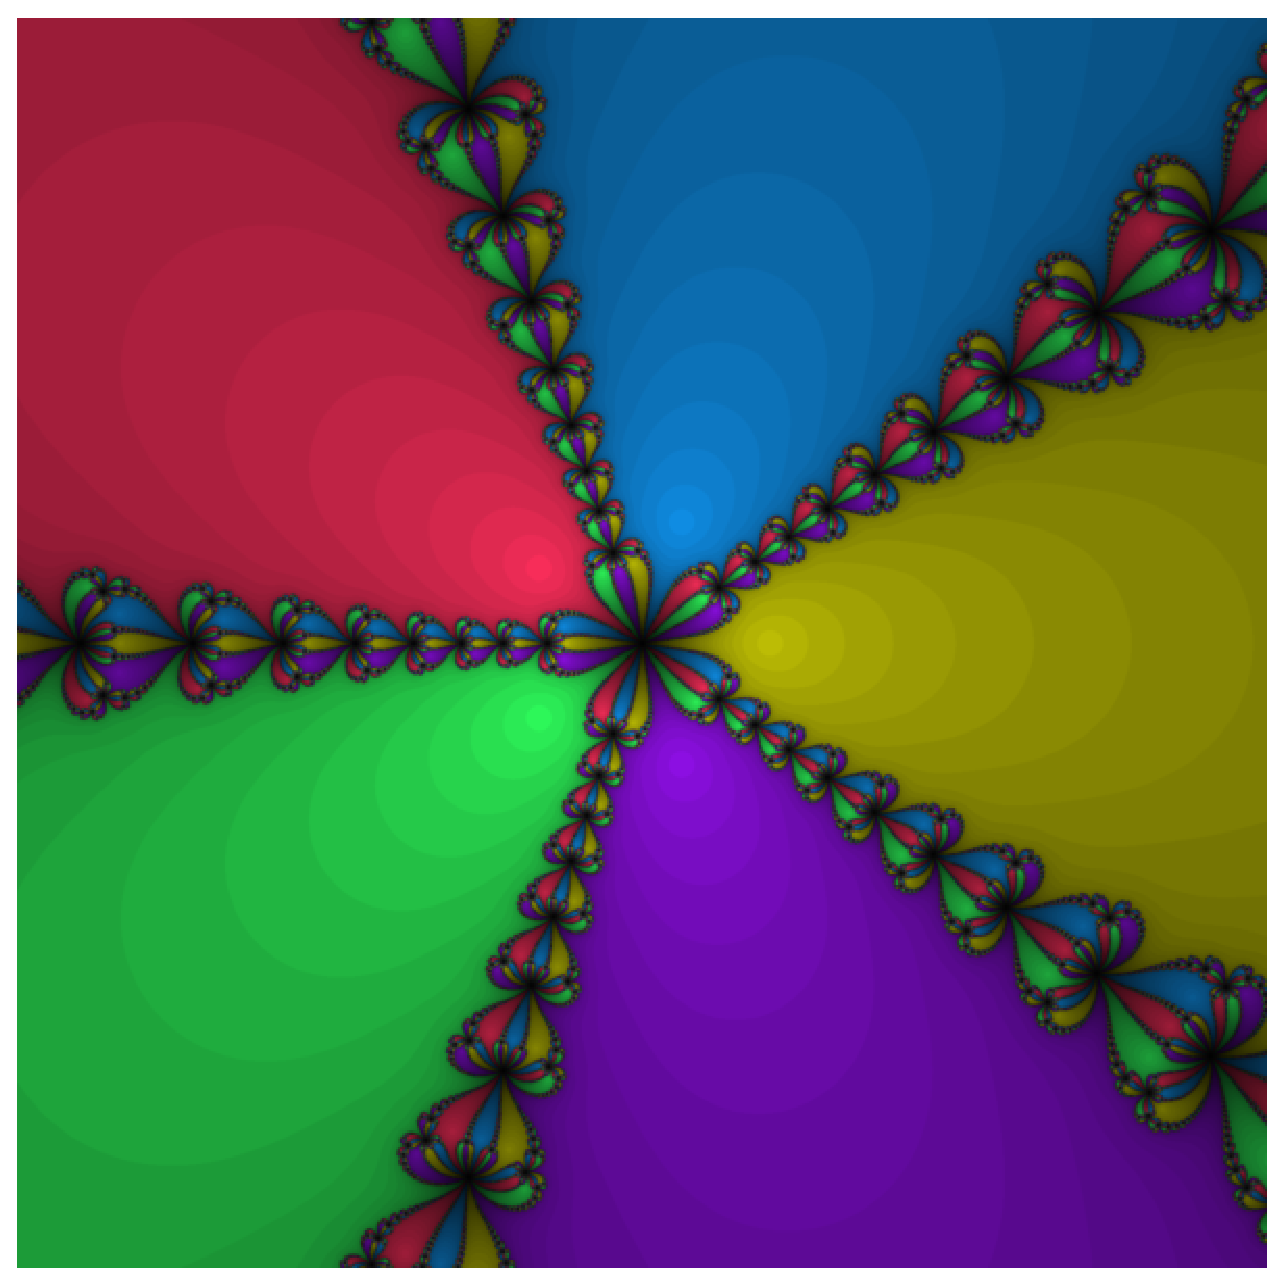
\includegraphics[height=9cm,width=9cm]{newtons-fractal.eps}%
\lthtmlpictureZ
\lthtmlcheckvsize\clearpage}

\stepcounter{chapter}
\stepcounter{section}
{\newpage\clearpage
\lthtmldisplayA{displaymath50901}%
\begin{displaymath}
\begin{array}{rl}
\  y 	&=\  3x^4,\\
\frac{dy}{dx} 	&=\  12x^3,\\
\frac{d}{dx} \left ( \frac{dy}{dx} \right ) 	&=\  36x^2,\\
\frac{d}{dx} \left [ \frac{d}{dx} \left ( \frac{dy}{dx} \right ) \right ] 	
&=\  72x,
\end{array}
\end{displaymath}%
\lthtmldisplayZ
\lthtmlcheckvsize\clearpage}

\stepcounter{section}
{\newpage\clearpage
\lthtmldisplayA{displaymath50904}%
\begin{displaymath}
\begin{array}{rl}
\frac{d}{dx} \left ( \frac{dy}{dx} \right ) 	&=\  \frac{d^2y}{dx^2},\\
\frac{d}{dx} \left [ \frac{d}{dx} \left ( \frac{dy}{dx} \right ) \right ] 	
&=\  \frac{d}{dx} \left ( \frac{d^2y}{dx^2} \right ) = \frac{d^3y}{dx^3},\\
. . . &	. . .\\
\frac{d}{dx} \left ( \frac{d^{n-1}y}{dx^{n-1}} \right )
 &	= \frac{d^ny}{dx^n}.
\end{array}
\end{displaymath}%
\lthtmldisplayZ
\lthtmlcheckvsize\clearpage}

{\newpage\clearpage
\lthtmlinlinemathA{tex2html_wrap_indisplay50908}%
$\displaystyle f'(x),\  f''(x),\  f'''(x),\  f^{(4)}(x),\  ...,\  f^{(n)}(x);
$%
\lthtmlindisplaymathZ
\lthtmlcheckvsize\clearpage}

{\newpage\clearpage
\lthtmlinlinemathA{tex2html_wrap_indisplay50910}%
$\displaystyle y',\  y'',\  y''',\  y^{(4)},\  ...,\  y^{(n)};
$%
\lthtmlindisplaymathZ
\lthtmlcheckvsize\clearpage}

{\newpage\clearpage
\lthtmlinlinemathA{tex2html_wrap_indisplay50912}%
$\displaystyle \frac{d}{dx} f(x),\  \frac{d^2}{dx^2} f(x),
\  \frac{d^3}{dx^3} f(x),\  \frac{d^4}{dx^4} f(x),
\  ...,\  \frac{d^n}{dx^n} f(x). 
$%
\lthtmlindisplaymathZ
\lthtmlcheckvsize\clearpage}

\stepcounter{section}
{\newpage\clearpage
\lthtmlinlinemathA{tex2html_wrap_inline50928}%
$ y = e^{ax}$%
\lthtmlinlinemathZ
\lthtmlcheckvsize\clearpage}

{\newpage\clearpage
\lthtmlinlinemathA{tex2html_wrap_inline50930}%
$ \frac{d^n y}{dx^n}$%
\lthtmlinlinemathZ
\lthtmlcheckvsize\clearpage}

{\newpage\clearpage
\lthtmlinlinemathA{tex2html_wrap_inline50932}%
$ \frac{dy}{dx} = ae^{ax}$%
\lthtmlinlinemathZ
\lthtmlcheckvsize\clearpage}

{\newpage\clearpage
\lthtmlinlinemathA{tex2html_wrap_inline50934}%
$ \frac{d^2 y}{dx^2} 	= a^2e^{ax}$%
\lthtmlinlinemathZ
\lthtmlcheckvsize\clearpage}

{\newpage\clearpage
\lthtmlinlinemathA{tex2html_wrap_inline50936}%
$ \frac{d^n y}{dx^n} = a^ne^{ax}$%
\lthtmlinlinemathZ
\lthtmlcheckvsize\clearpage}

{\newpage\clearpage
\lthtmlinlinemathA{tex2html_wrap_inline50943}%
$ y = \log\, x$%
\lthtmlinlinemathZ
\lthtmlcheckvsize\clearpage}

{\newpage\clearpage
\lthtmlinlinemathA{tex2html_wrap_inline50947}%
$ \frac{dy}{dx} 	= \frac{1}{x}$%
\lthtmlinlinemathZ
\lthtmlcheckvsize\clearpage}

{\newpage\clearpage
\lthtmlinlinemathA{tex2html_wrap_inline50949}%
$ \frac{d^2 y}{dx^2} 	= -\frac{1}{x^2}$%
\lthtmlinlinemathZ
\lthtmlcheckvsize\clearpage}

{\newpage\clearpage
\lthtmlinlinemathA{tex2html_wrap_inline50951}%
$ \frac{d^3 y}{dx^3} 	= \frac{1 \cdot 2}{x^3}$%
\lthtmlinlinemathZ
\lthtmlcheckvsize\clearpage}

{\newpage\clearpage
\lthtmlinlinemathA{tex2html_wrap_inline50953}%
$ \frac{d^4 y}{dx^4} 	= \frac{1 \cdot 2 \cdot 3}{x^4}$%
\lthtmlinlinemathZ
\lthtmlcheckvsize\clearpage}

{\newpage\clearpage
\lthtmlinlinemathA{tex2html_wrap_inline50955}%
$ \frac{d^n y}{dx^n} 	= (-1)^{n - 1} \frac{(n - 1)!}{x^n}$%
\lthtmlinlinemathZ
\lthtmlcheckvsize\clearpage}

{\newpage\clearpage
\lthtmlinlinemathA{tex2html_wrap_inline50966}%
$ \frac{dy}{dx} = \cos\, x = \sin \left ( x + \frac{\pi}{2} \right )$%
\lthtmlinlinemathZ
\lthtmlcheckvsize\clearpage}

{\newpage\clearpage
\lthtmlinlinemathA{tex2html_wrap_indisplay50968}%
$\displaystyle \frac{d^2 y}{dx^2} 
= \frac{d}{dx} \sin \left ( x + \frac{\pi}{2} \right ) 	
= \cos \left ( x + \frac{\pi}{2} \right ) 
= \sin \left ( x + \frac{2 \pi}{2} \right ),
$%
\lthtmlindisplaymathZ
\lthtmlcheckvsize\clearpage}

{\newpage\clearpage
\lthtmlinlinemathA{tex2html_wrap_indisplay50970}%
$\displaystyle \frac{d^3 y}{dx^3} 
= \frac{d}{dx} \sin \left ( x + \frac{2 \pi}{2} \right ) 	
= \cos \left ( x + \frac{2 \pi}{2} \right ) 
= \sin \left ( x + \frac{3 \pi}{2} \right )
$%
\lthtmlindisplaymathZ
\lthtmlcheckvsize\clearpage}

{\newpage\clearpage
\lthtmlinlinemathA{tex2html_wrap_indisplay50972}%
$\displaystyle \dots
$%
\lthtmlindisplaymathZ
\lthtmlcheckvsize\clearpage}

{\newpage\clearpage
\lthtmlinlinemathA{tex2html_wrap_indisplay50974}%
$\displaystyle \frac{d^n y}{dx^n} 	= \sin \left ( x + \frac{n \pi}{2} \right ).
$%
\lthtmlindisplaymathZ
\lthtmlcheckvsize\clearpage}

\stepcounter{section}
{\newpage\clearpage
\lthtmlinlinemathA{tex2html_wrap_indisplay50983}%
$\displaystyle \frac{d}{dx} (uv) = \frac{du}{dx} v + u \frac{dv}{dx}.
$%
\lthtmlindisplaymathZ
\lthtmlcheckvsize\clearpage}

{\newpage\clearpage
\lthtmlinlinemathA{tex2html_wrap_indisplay50987}%
$\displaystyle \frac{d^2}{dx^2}(uv) 
= \frac{d^2u}{dx^2}v + \frac{du}{dx} \frac{dv}{dx} 
+ \frac{du}{dx} \frac{dv}{dx} + u \frac{d^2 v}{dx^2} 
= \frac{d^2 u}{dx^2}v + 2 \frac{du}{dx} \frac{dv}{dx} 
+ u \frac{d^2 v}{dx^2}.
$%
\lthtmlindisplaymathZ
\lthtmlcheckvsize\clearpage}

{\newpage\clearpage
\lthtmldisplayA{displaymath50989}%
\begin{displaymath}
\begin{array}{ll}
\frac{d^3}{dx^3}(uv) 	
&= \frac{d^3 u}{dx^3} + \frac{d^2 u}{dx^2} \frac{dv}{dx} 
+ 2\frac{d^2 u}{dx^2} \frac{dv}{dx} + 2 \frac{du}{dx} \frac{d^2 v}{dx^2} 
+ \frac{du}{dx} \frac{d^2 v}{dx^2} + u \frac{d^3 v}{dx^3}\\
&= \frac{d^3 u}{dx^3}v + 3\frac{d^2 u}{dx^2} \frac{dv}{dx} 
+ 3 \frac{du}{dx} \frac{d^2 v}{dx^2} + u \frac{d^3 v}{dx^3}.
\end{array}
\end{displaymath}%
\lthtmldisplayZ
\lthtmlcheckvsize\clearpage}

{\newpage\clearpage
\lthtmlinlinemathA{tex2html_wrap_inline50997}%
$ \frac{d^0 u}{dx^0}$%
\lthtmlinlinemathZ
\lthtmlcheckvsize\clearpage}

{\newpage\clearpage
\lthtmlinlinemathA{tex2html_wrap_inline50999}%
$ \frac{d^0 v}{dx^0}$%
\lthtmlinlinemathZ
\lthtmlcheckvsize\clearpage}

{\newpage\clearpage
\lthtmlinlinemathA{tex2html_wrap_inline51003}%
$ (m + 1 )$%
\lthtmlinlinemathZ
\lthtmlcheckvsize\clearpage}

{\newpage\clearpage
\lthtmlinlinemathA{tex2html_wrap_indisplay51005}%
$\displaystyle \frac{d^n}{dx^n}(uv)  = \frac{d^n u}{dx^n} v + n \frac{d^{n - 1} u}{dx^{n - 1}} \frac{dv}{dx}  + \frac{n (n - 1)}{2!} \frac{d^{n - 2} u}{dx^{n - 2}} \frac{d^2 v}{dx^2}  + \cdots + n \frac{du}{dx} \frac{d^{n - 1} v}{dx^{n - 1}}  + u \frac{d^nv}{dx^n},$%
\lthtmlindisplaymathZ
\lthtmlcheckvsize\clearpage}

{\newpage\clearpage
\lthtmlinlinemathA{tex2html_wrap_inline51012}%
$ y = e^x\log\, x$%
\lthtmlinlinemathZ
\lthtmlcheckvsize\clearpage}

{\newpage\clearpage
\lthtmlinlinemathA{tex2html_wrap_inline51014}%
$ \frac{d^3 y}{dx^3}$%
\lthtmlinlinemathZ
\lthtmlcheckvsize\clearpage}

{\newpage\clearpage
\lthtmlinlinemathA{tex2html_wrap_inline51016}%
$ u = e^x$%
\lthtmlinlinemathZ
\lthtmlcheckvsize\clearpage}

{\newpage\clearpage
\lthtmlinlinemathA{tex2html_wrap_inline51018}%
$ v = \log\, x$%
\lthtmlinlinemathZ
\lthtmlcheckvsize\clearpage}

{\newpage\clearpage
\lthtmlinlinemathA{tex2html_wrap_inline51020}%
$ \frac{du}{dx} = e^x$%
\lthtmlinlinemathZ
\lthtmlcheckvsize\clearpage}

{\newpage\clearpage
\lthtmlinlinemathA{tex2html_wrap_inline51022}%
$ \frac{dv}{dx} = \frac{1}{x}$%
\lthtmlinlinemathZ
\lthtmlcheckvsize\clearpage}

{\newpage\clearpage
\lthtmlinlinemathA{tex2html_wrap_inline51024}%
$ \frac{d^2 u}{dx^2} = e^x$%
\lthtmlinlinemathZ
\lthtmlcheckvsize\clearpage}

{\newpage\clearpage
\lthtmlinlinemathA{tex2html_wrap_inline51026}%
$ \frac{d^2 v}{dx^2} = - \frac{1}{x^2}$%
\lthtmlinlinemathZ
\lthtmlcheckvsize\clearpage}

{\newpage\clearpage
\lthtmlinlinemathA{tex2html_wrap_inline51028}%
$ \frac{d^3 u}{dx^3} = e^x$%
\lthtmlinlinemathZ
\lthtmlcheckvsize\clearpage}

{\newpage\clearpage
\lthtmlinlinemathA{tex2html_wrap_inline51030}%
$ \frac{d^3 v}{dx^3} = \frac{2}{x^3}$%
\lthtmlinlinemathZ
\lthtmlcheckvsize\clearpage}

{\newpage\clearpage
\lthtmlinlinemathA{tex2html_wrap_indisplay51032}%
$\displaystyle \frac{d^3 y}{dx^3} = e^x \log x + \frac{3 e^x}{x} - \frac{3 e^x}{x^2} = e^x \left ( \log x + \frac{3}{x} - \frac{3}{x^2} + \frac{2}{x^3} \right ).
$%
\lthtmlindisplaymathZ
\lthtmlcheckvsize\clearpage}

{\newpage\clearpage
\lthtmlinlinemathA{tex2html_wrap_inline51039}%
$ y = x^2e^{ax}$%
\lthtmlinlinemathZ
\lthtmlcheckvsize\clearpage}

{\newpage\clearpage
\lthtmlinlinemathA{tex2html_wrap_inline51043}%
$ u = x^2$%
\lthtmlinlinemathZ
\lthtmlcheckvsize\clearpage}

{\newpage\clearpage
\lthtmlinlinemathA{tex2html_wrap_inline51045}%
$ v = e^{ax}$%
\lthtmlinlinemathZ
\lthtmlcheckvsize\clearpage}

{\newpage\clearpage
\lthtmlinlinemathA{tex2html_wrap_inline51047}%
$ \frac{du}{dx} = 2x$%
\lthtmlinlinemathZ
\lthtmlcheckvsize\clearpage}

{\newpage\clearpage
\lthtmlinlinemathA{tex2html_wrap_inline51049}%
$ \frac{dv}{dx} = ae^{ax}$%
\lthtmlinlinemathZ
\lthtmlcheckvsize\clearpage}

{\newpage\clearpage
\lthtmlinlinemathA{tex2html_wrap_inline51051}%
$ \frac{d^2 u}{dx^2} = 2x$%
\lthtmlinlinemathZ
\lthtmlcheckvsize\clearpage}

{\newpage\clearpage
\lthtmlinlinemathA{tex2html_wrap_inline51053}%
$ \frac{d^2 v}{dx^2} = a^2 e^{ax}$%
\lthtmlinlinemathZ
\lthtmlcheckvsize\clearpage}

{\newpage\clearpage
\lthtmlinlinemathA{tex2html_wrap_inline51055}%
$ \frac{d^3 u}{dx^3} = 0$%
\lthtmlinlinemathZ
\lthtmlcheckvsize\clearpage}

{\newpage\clearpage
\lthtmlinlinemathA{tex2html_wrap_inline51057}%
$ \frac{d^3 v}{dx^3} = a^3 e^{ax}$%
\lthtmlinlinemathZ
\lthtmlcheckvsize\clearpage}

{\newpage\clearpage
\lthtmlinlinemathA{tex2html_wrap_inline51059}%
$ \frac{d^n u}{dx^n} = 0$%
\lthtmlinlinemathZ
\lthtmlcheckvsize\clearpage}

{\newpage\clearpage
\lthtmlinlinemathA{tex2html_wrap_inline51061}%
$ \frac{d^n v}{dx^n} = a^n e^{ax}$%
\lthtmlinlinemathZ
\lthtmlcheckvsize\clearpage}

{\newpage\clearpage
\lthtmlinlinemathA{tex2html_wrap_indisplay51063}%
$\displaystyle \frac{d^n y}{dx^n} 
= x^2 a^n e^{ax} + 2na^{n - 1} x e^{ax} + n(n - 1)a^{n - 2} e^{ax} 
= a^{n - 2} e^{ax} [ x^2 a^2 + 2nax + n(n - 1) ].
$%
\lthtmlindisplaymathZ
\lthtmlcheckvsize\clearpage}

\stepcounter{section}
{\newpage\clearpage
\lthtmlinlinemathA{tex2html_wrap_inline51066}%
$ \frac{d^2 y}{dx^2}$%
\lthtmlinlinemathZ
\lthtmlcheckvsize\clearpage}

{\newpage\clearpage
\lthtmlinlinemathA{tex2html_wrap_indisplay51068}%
$\displaystyle b^2x^2 - a^2y^2 = a^2b^2.
$%
\lthtmlindisplaymathZ
\lthtmlcheckvsize\clearpage}

{\newpage\clearpage
\lthtmlinlinemathA{tex2html_wrap_indisplay51072}%
$\displaystyle 2b^2 x - 2a^2 y \frac{dy}{dx} = 0,
$%
\lthtmlindisplaymathZ
\lthtmlcheckvsize\clearpage}

{\newpage\clearpage
\lthtmlinlinemathA{tex2html_wrap_indisplay51074}%
$\displaystyle \frac{dy}{dx} = \frac{b^2 x}{a^2 y}.$%
\lthtmlindisplaymathZ
\lthtmlcheckvsize\clearpage}

{\newpage\clearpage
\lthtmlinlinemathA{tex2html_wrap_indisplay51080}%
$\displaystyle \frac{d^2 y}{dx^2} 
= \frac{a^2 y b^2 - b^2 x a^2 \frac{dy}{dx}}{a^4 y^2}.
$%
\lthtmlindisplaymathZ
\lthtmlcheckvsize\clearpage}

{\newpage\clearpage
\lthtmlinlinemathA{tex2html_wrap_indisplay51084}%
$\displaystyle \frac{d^2 y}{dx^2} 
= \frac{a^2 b^2 y - a^2 b^2 x \left ( \frac{b^2 y}{a^2 y} \right ) }{a^4 y^2} 
= -\frac{b^2 (b^2 x^2 - a^2 y^2)}{a^4 y^3}.
$%
\lthtmlindisplaymathZ
\lthtmlcheckvsize\clearpage}

{\newpage\clearpage
\lthtmlinlinemathA{tex2html_wrap_inline51086}%
$ b^2x^2 - a^2y^2 = a^2b^2$%
\lthtmlinlinemathZ
\lthtmlcheckvsize\clearpage}

{\newpage\clearpage
\lthtmlinlinemathA{tex2html_wrap_indisplay51088}%
$\displaystyle \frac{d^2 y}{dx^2} = - \frac{b^4}{a^2 y^3}. 
$%
\lthtmlindisplaymathZ
\lthtmlcheckvsize\clearpage}

{\newpage\clearpage
\lthtmlinlinemathA{tex2html_wrap_indisplay51090}%
$\displaystyle y'=\frac{d y}{dx} =  \frac{b^2x}{a^2 y},
$%
\lthtmlindisplaymathZ
\lthtmlcheckvsize\clearpage}

{\newpage\clearpage
\lthtmlinlinemathA{tex2html_wrap_indisplay51092}%
$\displaystyle y''=\frac{d^2 y}{dx^2} = - \frac{b^2-a^2(y')^2}{a^2 y}. 
$%
\lthtmlindisplaymathZ
\lthtmlcheckvsize\clearpage}

{\newpage\clearpage
\lthtmlinlinemathA{tex2html_wrap_inline51094}%
$ y''=-b^2\frac{1-a^{-2}b^2x^2/y^2}{a^2y}$%
\lthtmlinlinemathZ
\lthtmlcheckvsize\clearpage}

{\newpage\clearpage
\lthtmlinlinemathA{tex2html_wrap_inline51096}%
$ a^{-2}b^2x^2/y^2-1=b^2/y^2$%
\lthtmlinlinemathZ
\lthtmlcheckvsize\clearpage}

\stepcounter{section}
{\newpage\clearpage
\lthtmlinlinemathA{tex2html_wrap_inline51099}%
$ y = 4x^3 - 6x^2 + 4x + 7$%
\lthtmlinlinemathZ
\lthtmlcheckvsize\clearpage}

{\newpage\clearpage
\lthtmlinlinemathA{tex2html_wrap_inline51101}%
$ \frac{d^2 y}{dx^2} = 12(2x - 1)$%
\lthtmlinlinemathZ
\lthtmlcheckvsize\clearpage}

{\newpage\clearpage
\lthtmlinlinemathA{tex2html_wrap_inline51103}%
$ f(x) = \frac{x^3}{1 - x}$%
\lthtmlinlinemathZ
\lthtmlcheckvsize\clearpage}

{\newpage\clearpage
\lthtmlinlinemathA{tex2html_wrap_inline51105}%
$ f^{(4)}(x) = \frac{4!}{(1 - x)^5}$%
\lthtmlinlinemathZ
\lthtmlcheckvsize\clearpage}

{\newpage\clearpage
\lthtmlinlinemathA{tex2html_wrap_inline51107}%
$ f(y) = y^6$%
\lthtmlinlinemathZ
\lthtmlcheckvsize\clearpage}

{\newpage\clearpage
\lthtmlinlinemathA{tex2html_wrap_inline51109}%
$ f^{(6)}(y) = 6!$%
\lthtmlinlinemathZ
\lthtmlcheckvsize\clearpage}

{\newpage\clearpage
\lthtmlinlinemathA{tex2html_wrap_inline51111}%
$ y = x^3\log\, x$%
\lthtmlinlinemathZ
\lthtmlcheckvsize\clearpage}

{\newpage\clearpage
\lthtmlinlinemathA{tex2html_wrap_inline51113}%
$ \frac{d^4 y}{dx^4} = \frac{6}{x}$%
\lthtmlinlinemathZ
\lthtmlcheckvsize\clearpage}

{\newpage\clearpage
\lthtmlinlinemathA{tex2html_wrap_inline51115}%
$ y = \frac{c}{x^n}$%
\lthtmlinlinemathZ
\lthtmlcheckvsize\clearpage}

{\newpage\clearpage
\lthtmlinlinemathA{tex2html_wrap_inline51117}%
$ y'' = \frac{n(n + 1)c}{x^{n + 2}}$%
\lthtmlinlinemathZ
\lthtmlcheckvsize\clearpage}

{\newpage\clearpage
\lthtmlinlinemathA{tex2html_wrap_inline51119}%
$ y = (x - 3)e^{2x} + 4xe^x + x$%
\lthtmlinlinemathZ
\lthtmlcheckvsize\clearpage}

{\newpage\clearpage
\lthtmlinlinemathA{tex2html_wrap_inline51121}%
$ y'' = 4e^x[(x - 2)e^x + x + 2]$%
\lthtmlinlinemathZ
\lthtmlcheckvsize\clearpage}

{\newpage\clearpage
\lthtmlinlinemathA{tex2html_wrap_inline51125}%
$ y'' = \frac{1}{2a} (e^{\frac{x}{a}} + e^{-\frac{x}{a}}) = \frac{y}{a^2}$%
\lthtmlinlinemathZ
\lthtmlcheckvsize\clearpage}

{\newpage\clearpage
\lthtmlinlinemathA{tex2html_wrap_inline51127}%
$ f(x) = ax^2 + bx + c$%
\lthtmlinlinemathZ
\lthtmlcheckvsize\clearpage}

{\newpage\clearpage
\lthtmlinlinemathA{tex2html_wrap_inline51129}%
$ f'''(x) = 0$%
\lthtmlinlinemathZ
\lthtmlcheckvsize\clearpage}

{\newpage\clearpage
\lthtmlinlinemathA{tex2html_wrap_inline51131}%
$ f(x) = \log(x + 1)$%
\lthtmlinlinemathZ
\lthtmlcheckvsize\clearpage}

{\newpage\clearpage
\lthtmlinlinemathA{tex2html_wrap_inline51133}%
$ f^{(4)} (x) = -\frac{6}{(x + 1)^4}$%
\lthtmlinlinemathZ
\lthtmlcheckvsize\clearpage}

{\newpage\clearpage
\lthtmlinlinemathA{tex2html_wrap_inline51135}%
$ f(x) = log(e^x + e^{-x})$%
\lthtmlinlinemathZ
\lthtmlcheckvsize\clearpage}

{\newpage\clearpage
\lthtmlinlinemathA{tex2html_wrap_inline51137}%
$ f'''(x) = -\frac{8(e^x - e^{-x})}{(e^x - e^{-x})^3}$%
\lthtmlinlinemathZ
\lthtmlcheckvsize\clearpage}

{\newpage\clearpage
\lthtmlinlinemathA{tex2html_wrap_inline51139}%
$ r = \sin\, a\theta$%
\lthtmlinlinemathZ
\lthtmlcheckvsize\clearpage}

{\newpage\clearpage
\lthtmlinlinemathA{tex2html_wrap_inline51141}%
$ \frac{d^4 r}{d\theta^4} = a^4 \sin a\theta = a^4 r$%
\lthtmlinlinemathZ
\lthtmlcheckvsize\clearpage}

{\newpage\clearpage
\lthtmlinlinemathA{tex2html_wrap_inline51143}%
$ r = \tan\, \phi$%
\lthtmlinlinemathZ
\lthtmlcheckvsize\clearpage}

{\newpage\clearpage
\lthtmlinlinemathA{tex2html_wrap_inline51145}%
$ \frac{d^3 r}{d\phi^3} = 6 \sec^6 \phi - 4 \sec^2 \phi$%
\lthtmlinlinemathZ
\lthtmlcheckvsize\clearpage}

{\newpage\clearpage
\lthtmlinlinemathA{tex2html_wrap_inline51147}%
$ r = \log\sin\, \phi$%
\lthtmlinlinemathZ
\lthtmlcheckvsize\clearpage}

{\newpage\clearpage
\lthtmlinlinemathA{tex2html_wrap_inline51149}%
$ r''' = 2\cot\,\phi \csc^2\phi$%
\lthtmlinlinemathZ
\lthtmlcheckvsize\clearpage}

{\newpage\clearpage
\lthtmlinlinemathA{tex2html_wrap_inline51151}%
$ f(t) = e^{-t}\cos\, t$%
\lthtmlinlinemathZ
\lthtmlcheckvsize\clearpage}

{\newpage\clearpage
\lthtmlinlinemathA{tex2html_wrap_inline51153}%
$ f^{(4)}(t) = - 4e^{- t}\cos\, t = - 4f(t)$%
\lthtmlinlinemathZ
\lthtmlcheckvsize\clearpage}

{\newpage\clearpage
\lthtmlinlinemathA{tex2html_wrap_inline51155}%
$ f(\theta) = \sqrt{\sec 2\theta}$%
\lthtmlinlinemathZ
\lthtmlcheckvsize\clearpage}

{\newpage\clearpage
\lthtmlinlinemathA{tex2html_wrap_inline51157}%
$ f''(\theta) = 3[f(\theta)]5 - f(\theta)$%
\lthtmlinlinemathZ
\lthtmlcheckvsize\clearpage}

{\newpage\clearpage
\lthtmlinlinemathA{tex2html_wrap_inline51159}%
$ p = (q^2 + a^2) \arctan \frac{q}{a}$%
\lthtmlinlinemathZ
\lthtmlcheckvsize\clearpage}

{\newpage\clearpage
\lthtmlinlinemathA{tex2html_wrap_inline51161}%
$ \frac{d^3 p}{dq^3} = \frac{4a^3}{(a^2 + q^2)^2}$%
\lthtmlinlinemathZ
\lthtmlcheckvsize\clearpage}

{\newpage\clearpage
\lthtmlinlinemathA{tex2html_wrap_inline51165}%
$ \frac{d^n y}{dx^n} = (\log a)^n a^x$%
\lthtmlinlinemathZ
\lthtmlcheckvsize\clearpage}

{\newpage\clearpage
\lthtmlinlinemathA{tex2html_wrap_inline51167}%
$ y = \log(1 + x)$%
\lthtmlinlinemathZ
\lthtmlcheckvsize\clearpage}

{\newpage\clearpage
\lthtmlinlinemathA{tex2html_wrap_inline51169}%
$ \frac{d^n y}{dx^n} = (-1)^{n - 1} \frac{(n - 1)!}{(1 + x)^n}$%
\lthtmlinlinemathZ
\lthtmlcheckvsize\clearpage}

{\newpage\clearpage
\lthtmlinlinemathA{tex2html_wrap_inline51171}%
$ y = \cos\, ax$%
\lthtmlinlinemathZ
\lthtmlcheckvsize\clearpage}

{\newpage\clearpage
\lthtmlinlinemathA{tex2html_wrap_inline51173}%
$ \frac{d^n y}{dx^n} = a^n \cos \left ( ax + \frac{n\pi}{2} \right )$%
\lthtmlinlinemathZ
\lthtmlcheckvsize\clearpage}

{\newpage\clearpage
\lthtmlinlinemathA{tex2html_wrap_inline51175}%
$ y = x^{n- 1}\log\, x$%
\lthtmlinlinemathZ
\lthtmlcheckvsize\clearpage}

{\newpage\clearpage
\lthtmlinlinemathA{tex2html_wrap_inline51177}%
$ \frac{d^n y}{dx^n} = \frac{(n - 1)!}{x}$%
\lthtmlinlinemathZ
\lthtmlcheckvsize\clearpage}

{\newpage\clearpage
\lthtmlinlinemathA{tex2html_wrap_inline51179}%
$ y = \frac{1 - x}{1 + x}$%
\lthtmlinlinemathZ
\lthtmlcheckvsize\clearpage}

{\newpage\clearpage
\lthtmlinlinemathA{tex2html_wrap_inline51181}%
$ \frac{d^n y}{dx^n} = 2 (-1)^n \frac{n!}{(1 + x)^{n + 1}}$%
\lthtmlinlinemathZ
\lthtmlcheckvsize\clearpage}

{\newpage\clearpage
\lthtmlinlinemathA{tex2html_wrap_inline51183}%
$ -1 + \frac{2}{1 + x}$%
\lthtmlinlinemathZ
\lthtmlcheckvsize\clearpage}

{\newpage\clearpage
\lthtmlinlinemathA{tex2html_wrap_inline51185}%
$ y = e^x\sin\, x$%
\lthtmlinlinemathZ
\lthtmlcheckvsize\clearpage}

{\newpage\clearpage
\lthtmlinlinemathA{tex2html_wrap_inline51187}%
$ \frac{d^2 y}{dx^2} - 2 \frac{dy}{dx} + 2y = 0$%
\lthtmlinlinemathZ
\lthtmlcheckvsize\clearpage}

{\newpage\clearpage
\lthtmlinlinemathA{tex2html_wrap_inline51189}%
$ y = a\cos(\log\, x) + b\sin(\log\, x)$%
\lthtmlinlinemathZ
\lthtmlcheckvsize\clearpage}

{\newpage\clearpage
\lthtmlinlinemathA{tex2html_wrap_inline51191}%
$ x^2 \frac{d^2 y}{dx^2} + x \frac{dy}{dx} + y = 0$%
\lthtmlinlinemathZ
\lthtmlcheckvsize\clearpage}

\addtocounter{enumi}{23}
{\newpage\clearpage
\lthtmlinlinemathA{tex2html_wrap_inline51193}%
$ y = x^2a^x$%
\lthtmlinlinemathZ
\lthtmlcheckvsize\clearpage}

{\newpage\clearpage
\lthtmlinlinemathA{tex2html_wrap_inline51195}%
$ \frac{d^n y}{dx^n} = a^x (\log a)^{n - 2} [(x \log a + n)^2 - n]$%
\lthtmlinlinemathZ
\lthtmlcheckvsize\clearpage}

{\newpage\clearpage
\lthtmlinlinemathA{tex2html_wrap_inline51197}%
$ y = xe^x$%
\lthtmlinlinemathZ
\lthtmlcheckvsize\clearpage}

{\newpage\clearpage
\lthtmlinlinemathA{tex2html_wrap_inline51199}%
$ \frac{d^n y}{dx^n} = (x + n)e^x$%
\lthtmlinlinemathZ
\lthtmlcheckvsize\clearpage}

{\newpage\clearpage
\lthtmlinlinemathA{tex2html_wrap_inline51201}%
$ f(x) = e^x\sin\, x$%
\lthtmlinlinemathZ
\lthtmlcheckvsize\clearpage}

{\newpage\clearpage
\lthtmlinlinemathA{tex2html_wrap_inline51203}%
$ f^{(n)}(x) = (\sqrt{2})^n e^x \sin \left ( x + \frac{n\pi}{4} \right )$%
\lthtmlinlinemathZ
\lthtmlcheckvsize\clearpage}

{\newpage\clearpage
\lthtmlinlinemathA{tex2html_wrap_inline51205}%
$ f(\theta) = \cos\,a\theta\cos\,b\theta$%
\lthtmlinlinemathZ
\lthtmlcheckvsize\clearpage}

{\newpage\clearpage
\lthtmlinlinemathA{tex2html_wrap_inline51207}%
$ f^{n}(\theta) 
= \frac{(a + b)^n}{2} \cos \left [ (a + b)\theta + \frac{n\pi}{2} \right ]
+ \frac{(a - b)^n}{2} \cos \left [ (a - b)\theta + \frac{n\pi}{2} \right ]$%
\lthtmlinlinemathZ
\lthtmlcheckvsize\clearpage}

{\newpage\clearpage
\lthtmlinlinemathA{tex2html_wrap_inline51209}%
$ a = \frac{d^2 s}{dt^2}$%
\lthtmlinlinemathZ
\lthtmlcheckvsize\clearpage}

{\newpage\clearpage
\lthtmlinlinemathA{tex2html_wrap_inline51211}%
$ a_x = \frac{d^2 x}{dt^2}$%
\lthtmlinlinemathZ
\lthtmlcheckvsize\clearpage}

{\newpage\clearpage
\lthtmlinlinemathA{tex2html_wrap_inline51213}%
$ a_y = \frac{d^2 y}{dt^2}$%
\lthtmlinlinemathZ
\lthtmlcheckvsize\clearpage}

{\newpage\clearpage
\lthtmlinlinemathA{tex2html_wrap_inline51215}%
$ y^2 = 4ax$%
\lthtmlinlinemathZ
\lthtmlcheckvsize\clearpage}

{\newpage\clearpage
\lthtmlinlinemathA{tex2html_wrap_inline51217}%
$ \frac{d^2 y}{dx^2} = -\frac{4a^2}{y^3}$%
\lthtmlinlinemathZ
\lthtmlcheckvsize\clearpage}

{\newpage\clearpage
\lthtmlinlinemathA{tex2html_wrap_inline51221}%
$ \frac{d^2 y}{dx^2} = -\frac{b^4}{a^2 y^3}$%
\lthtmlinlinemathZ
\lthtmlcheckvsize\clearpage}

{\newpage\clearpage
\lthtmlinlinemathA{tex2html_wrap_inline51223}%
$ \frac{d^3 y}{dx^2} = -\frac{3b^6 x}{a^4 y^5}$%
\lthtmlinlinemathZ
\lthtmlcheckvsize\clearpage}

{\newpage\clearpage
\lthtmlinlinemathA{tex2html_wrap_inline51227}%
$ \frac{d^2 y}{dx^2} = -\frac{r^2}{y^3}$%
\lthtmlinlinemathZ
\lthtmlcheckvsize\clearpage}

{\newpage\clearpage
\lthtmlinlinemathA{tex2html_wrap_inline51229}%
$ y^2 + y = x^2$%
\lthtmlinlinemathZ
\lthtmlcheckvsize\clearpage}

{\newpage\clearpage
\lthtmlinlinemathA{tex2html_wrap_inline51231}%
$ \frac{d^3 y}{dx^3} = -\frac{24x}{(1 + 2y)^5}$%
\lthtmlinlinemathZ
\lthtmlcheckvsize\clearpage}

{\newpage\clearpage
\lthtmlinlinemathA{tex2html_wrap_inline51233}%
$ ax^2 + 2hxy + by^2 = 1$%
\lthtmlinlinemathZ
\lthtmlcheckvsize\clearpage}

{\newpage\clearpage
\lthtmlinlinemathA{tex2html_wrap_inline51235}%
$ \frac{d^2 y}{dx^2} = \frac{h^2 - ab}{(hx + by)^3}$%
\lthtmlinlinemathZ
\lthtmlcheckvsize\clearpage}

{\newpage\clearpage
\lthtmlinlinemathA{tex2html_wrap_inline51237}%
$ y^2 - 2xy = a^2$%
\lthtmlinlinemathZ
\lthtmlcheckvsize\clearpage}

{\newpage\clearpage
\lthtmlinlinemathA{tex2html_wrap_inline51239}%
$ \frac{d^2 y}{dx^2} 
= \frac{a^2}{(y - x)^3}; \frac{d^3 y}{dx^3} = -\frac{3a^2 x}{(y - x)^5}$%
\lthtmlinlinemathZ
\lthtmlcheckvsize\clearpage}

{\newpage\clearpage
\lthtmlinlinemathA{tex2html_wrap_inline51241}%
$ \sec\,\phi\cos\,\theta = c$%
\lthtmlinlinemathZ
\lthtmlcheckvsize\clearpage}

{\newpage\clearpage
\lthtmlinlinemathA{tex2html_wrap_inline51243}%
$ \frac{d^2 \theta}{d\phi^2} = \frac{\tan^2 \theta - \tan^2 \phi}{\tan^3 \theta}$%
\lthtmlinlinemathZ
\lthtmlcheckvsize\clearpage}

{\newpage\clearpage
\lthtmlinlinemathA{tex2html_wrap_inline51245}%
$ \theta=\tan(\phi + \theta)$%
\lthtmlinlinemathZ
\lthtmlcheckvsize\clearpage}

{\newpage\clearpage
\lthtmlinlinemathA{tex2html_wrap_inline51247}%
$ \frac{d^3 \theta}{d\phi^3} = -\frac{2(5 + 8\theta^2 + 3\theta^4)}{\theta^8}$%
\lthtmlinlinemathZ
\lthtmlcheckvsize\clearpage}

{\newpage\clearpage
\lthtmldisplayA{displaymath51249}%
\begin{displaymath}
\begin{array}{ll}
(a)\  \  \log(u + v) = u - v. &	(e)\  \  y^3 + x^3 - 3axy = 0.\\
(b)\  \  e^u + u = e^v + v.  &	(f)\  \  y^2 - 2mxy + x^2 - a = 0.\\
(c)\  \  s = 1 + te^s.  &	(g)\  \  y = \sin(x + y).\\
(d)\  \  e^s + st - e = 0.  &	(h)\  \  e^{x + y} = xy.\\
\end{array}
\end{displaymath}%
\lthtmldisplayZ
\lthtmlcheckvsize\clearpage}

\stepcounter{chapter}
\stepcounter{section}
{\newpage\clearpage
\lthtmlpictureA{tex2html_wrap51262}%

% latex2html id marker 51262
\includegraphics[height=6cm,width=6cm]{circle-example3.eps}%
\lthtmlpictureZ
\lthtmlcheckvsize\clearpage}

{\newpage\clearpage
\lthtmlinlinemathA{tex2html_wrap_inline51267}%
$ CD = x$%
\lthtmlinlinemathZ
\lthtmlcheckvsize\clearpage}

{\newpage\clearpage
\lthtmlinlinemathA{tex2html_wrap_inline51269}%
$ DE = \sqrt{100 - x^2}$%
\lthtmlinlinemathZ
\lthtmlcheckvsize\clearpage}

{\newpage\clearpage
\lthtmlinlinemathA{tex2html_wrap_indisplay51271}%
$\displaystyle A = A(x) = x\sqrt{100 - x^2}.
$%
\lthtmlindisplaymathZ
\lthtmlcheckvsize\clearpage}

{\newpage\clearpage
\lthtmlinlinemathA{tex2html_wrap_inline51275}%
$ = x$%
\lthtmlinlinemathZ
\lthtmlcheckvsize\clearpage}

{\newpage\clearpage
\lthtmlinlinemathA{tex2html_wrap_inline51279}%
$ DE$%
\lthtmlinlinemathZ
\lthtmlcheckvsize\clearpage}

{\newpage\clearpage
\lthtmlinlinemathA{tex2html_wrap_inline51281}%
$ = \sqrt{100 - x^2}$%
\lthtmlinlinemathZ
\lthtmlcheckvsize\clearpage}

{\newpage\clearpage
\lthtmlinlinemathA{tex2html_wrap_inline51285}%
$ A=A(x)$%
\lthtmlinlinemathZ
\lthtmlcheckvsize\clearpage}

{\newpage\clearpage
\lthtmlinlinemathA{tex2html_wrap_inline51287}%
$ A(x)$%
\lthtmlinlinemathZ
\lthtmlcheckvsize\clearpage}

{\newpage\clearpage
\lthtmlpictureA{tex2html_wrap51301}%

% latex2html id marker 51301
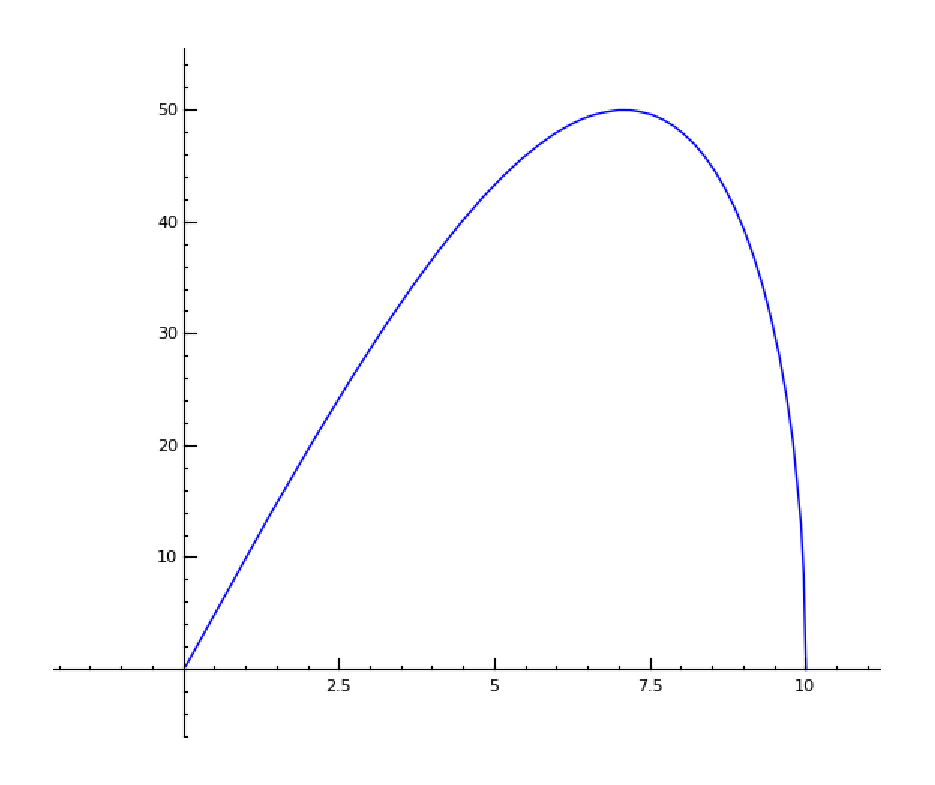
\includegraphics[height=4cm,width=7cm]{circle-example2.eps}%
\lthtmlpictureZ
\lthtmlcheckvsize\clearpage}

{\newpage\clearpage
\lthtmlinlinemathA{tex2html_wrap_inline51308}%
$ x = OM = 3$%
\lthtmlinlinemathZ
\lthtmlcheckvsize\clearpage}

{\newpage\clearpage
\lthtmlinlinemathA{tex2html_wrap_inline51310}%
$ A = MP = 28.6$%
\lthtmlinlinemathZ
\lthtmlcheckvsize\clearpage}

{\newpage\clearpage
\lthtmlinlinemathA{tex2html_wrap_inline51312}%
$ x = ON = \frac{9}{2}$%
\lthtmlinlinemathZ
\lthtmlcheckvsize\clearpage}

{\newpage\clearpage
\lthtmlinlinemathA{tex2html_wrap_inline51314}%
$ A = NQ \approx 39.8$%
\lthtmlinlinemathZ
\lthtmlcheckvsize\clearpage}

{\newpage\clearpage
\lthtmldisplayA{displaymath51322}%
\begin{displaymath}
\begin{array}{ll}
\  A 	&= x\sqrt{100 - x^2},\\
  \frac{dA}{dx} &=\  \frac{100 - 2 x^2}{\sqrt{100 - x^2}},\\
  \frac{100 - 2 x^2}{\sqrt{100 - x^2}} 	&=\  0.
\end{array}
\end{displaymath}%
\lthtmldisplayZ
\lthtmlcheckvsize\clearpage}

{\newpage\clearpage
\lthtmlinlinemathA{tex2html_wrap_inline51324}%
$ x 	=\  5\sqrt{2}$%
\lthtmlinlinemathZ
\lthtmlcheckvsize\clearpage}

{\newpage\clearpage
\lthtmlinlinemathA{tex2html_wrap_inline51326}%
$ DE 	= \sqrt{100 - x^2} = 5\sqrt{2}$%
\lthtmlinlinemathZ
\lthtmlcheckvsize\clearpage}

{\newpage\clearpage
\lthtmlinlinemathA{tex2html_wrap_inline51328}%
$ A = CD \times DE = 5\sqrt{2} \times 5\sqrt{2} = 50$%
\lthtmlinlinemathZ
\lthtmlcheckvsize\clearpage}

{\newpage\clearpage
\lthtmlinlinemathA{tex2html_wrap_inline51330}%
$ 50$%
\lthtmlinlinemathZ
\lthtmlcheckvsize\clearpage}

{\newpage\clearpage
\lthtmlinlinemathA{tex2html_wrap_inline51337}%
$ 108$%
\lthtmlinlinemathZ
\lthtmlcheckvsize\clearpage}

{\newpage\clearpage
\lthtmlpictureA{tex2html_wrap51339}%
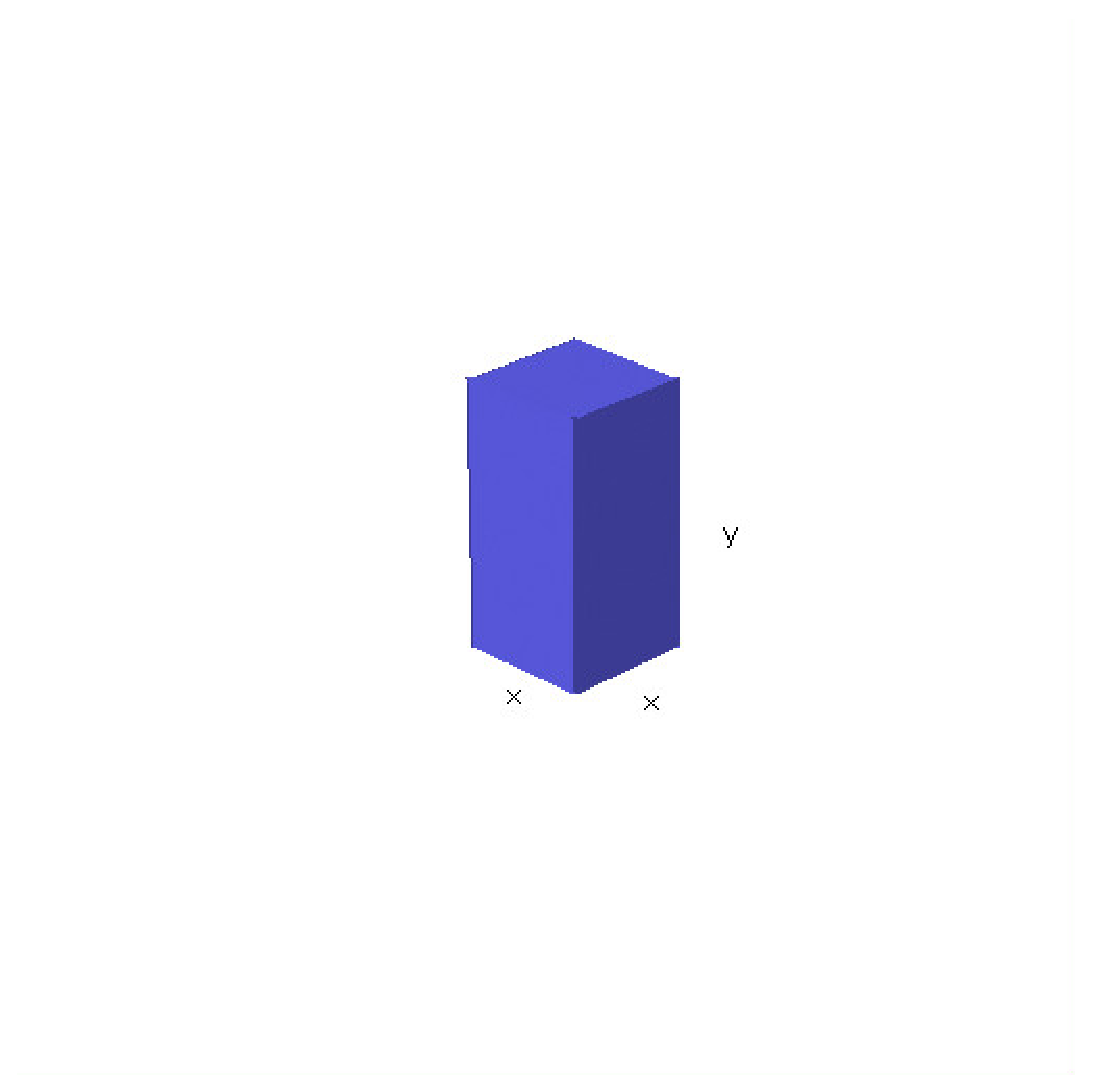
\includegraphics[height=6cm,width=5cm]{volume-box3b.eps}%
\lthtmlpictureZ
\lthtmlcheckvsize\clearpage}

{\newpage\clearpage
\lthtmlinlinemathA{tex2html_wrap_inline51360}%
$ {\rm volume} =\  x^2 y\  =\  108$%
\lthtmlinlinemathZ
\lthtmlcheckvsize\clearpage}

{\newpage\clearpage
\lthtmlinlinemathA{tex2html_wrap_inline51362}%
$ y\  =\  \frac{108}{x^2}$%
\lthtmlinlinemathZ
\lthtmlcheckvsize\clearpage}

{\newpage\clearpage
\lthtmlinlinemathA{tex2html_wrap_inline51370}%
$ 4xy\  =\  \frac{432}{x}$%
\lthtmlinlinemathZ
\lthtmlcheckvsize\clearpage}

{\newpage\clearpage
\lthtmlinlinemathA{tex2html_wrap_indisplay51372}%
$\displaystyle M = M(x)	=\  x^2 + \frac{432}{x}
$%
\lthtmlindisplaymathZ
\lthtmlcheckvsize\clearpage}

{\newpage\clearpage
\lthtmlinlinemathA{tex2html_wrap_inline51376}%
$ M(x)$%
\lthtmlinlinemathZ
\lthtmlcheckvsize\clearpage}

{\newpage\clearpage
\lthtmlpictureA{tex2html_wrap51378}%
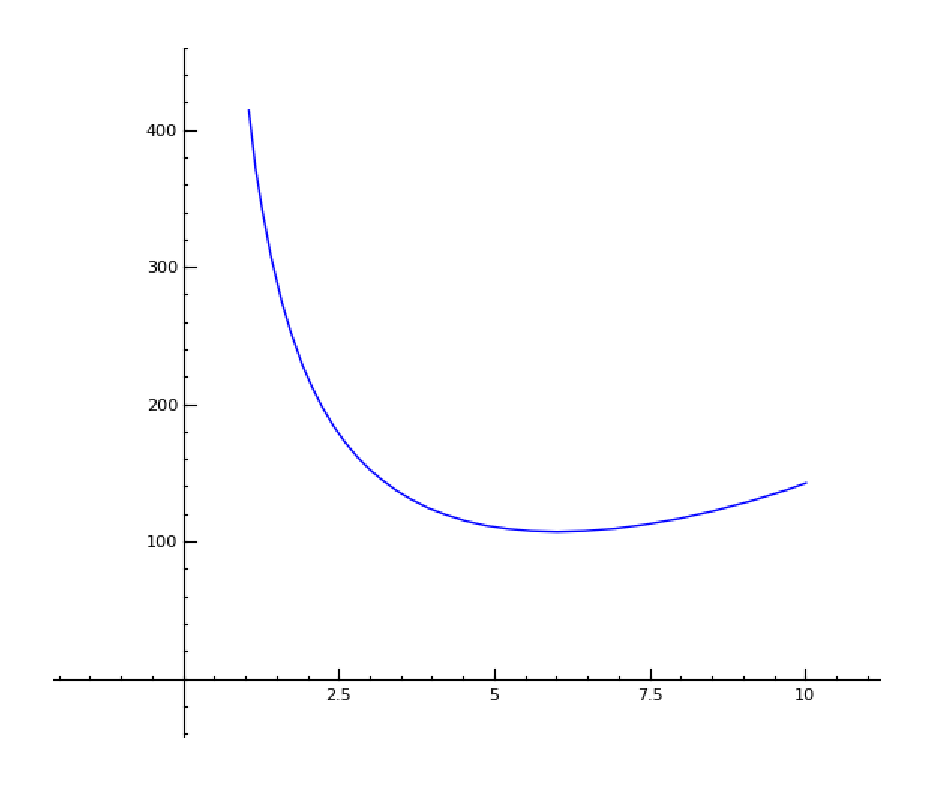
\includegraphics[height=4cm,width=7cm]{volume-box2.eps}%
\lthtmlpictureZ
\lthtmlcheckvsize\clearpage}

{\newpage\clearpage
\lthtmlinlinemathA{tex2html_wrap_inline51393}%
$ M=M(x)$%
\lthtmlinlinemathZ
\lthtmlcheckvsize\clearpage}

{\newpage\clearpage
\lthtmlinlinemathA{tex2html_wrap_indisplay51397}%
$\displaystyle \frac{dM}{dx} = 2x - \frac{432}{x^2}.
$%
\lthtmlindisplaymathZ
\lthtmlcheckvsize\clearpage}

{\newpage\clearpage
\lthtmlinlinemathA{tex2html_wrap_indisplay51399}%
$\displaystyle 2x - \frac{432}{x^2} = 0;
$%
\lthtmlindisplaymathZ
\lthtmlcheckvsize\clearpage}

{\newpage\clearpage
\lthtmlinlinemathA{tex2html_wrap_inline51401}%
$ x = 6$%
\lthtmlinlinemathZ
\lthtmlcheckvsize\clearpage}

{\newpage\clearpage
\lthtmlinlinemathA{tex2html_wrap_inline51405}%
$ M = 108$%
\lthtmlinlinemathZ
\lthtmlcheckvsize\clearpage}

{\newpage\clearpage
\lthtmlinlinemathA{tex2html_wrap_inline51411}%
$ (x^2 + 432/x)'=0$%
\lthtmlinlinemathZ
\lthtmlcheckvsize\clearpage}

\stepcounter{section}
{\newpage\clearpage
\lthtmlinlinemathA{tex2html_wrap_inline51423}%
$ a^x$%
\lthtmlinlinemathZ
\lthtmlcheckvsize\clearpage}

{\newpage\clearpage
\lthtmlpictureA{tex2html_wrap51429}%
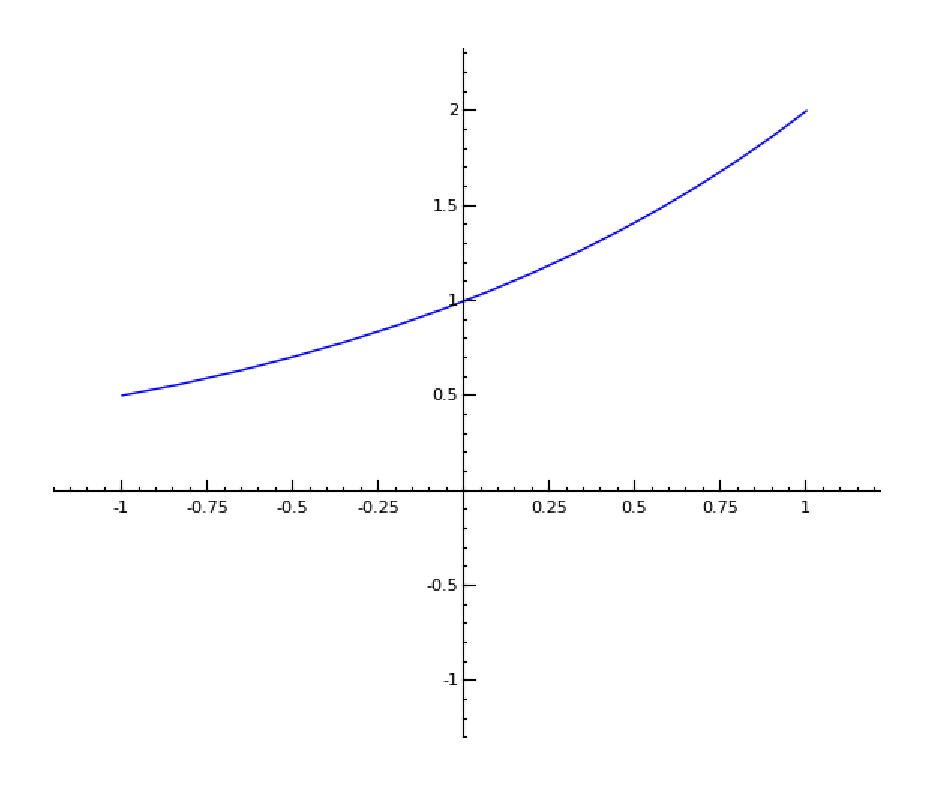
\includegraphics[height=4cm,width=4cm]{exp-fcn2.eps}%
\lthtmlpictureZ
\lthtmlcheckvsize\clearpage}

{\newpage\clearpage
\lthtmlinlinemathA{tex2html_wrap_inline51444}%
$ = y$%
\lthtmlinlinemathZ
\lthtmlcheckvsize\clearpage}

{\newpage\clearpage
\lthtmlinlinemathA{tex2html_wrap_inline51450}%
$ (a - x)^3$%
\lthtmlinlinemathZ
\lthtmlcheckvsize\clearpage}

{\newpage\clearpage
\lthtmlinlinemathA{tex2html_wrap_inline51452}%
$ y = (a - x)^3$%
\lthtmlinlinemathZ
\lthtmlcheckvsize\clearpage}

{\newpage\clearpage
\lthtmlpictureA{tex2html_wrap51454}%
\includegraphics[height=4cm,width=7cm]{cubic-fcn2.eps}%
\lthtmlpictureZ
\lthtmlcheckvsize\clearpage}

{\newpage\clearpage
\lthtmlinlinemathA{tex2html_wrap_indisplay51475}%
$\displaystyle y = 2x^3 - 9x^2 + 12x - 3.
$%
\lthtmlindisplaymathZ
\lthtmlcheckvsize\clearpage}

{\newpage\clearpage
\lthtmlpictureA{tex2html_wrap51477}%
\includegraphics[height=4cm,width=7cm]{cubic-fcn3.eps}%
\lthtmlpictureZ
\lthtmlcheckvsize\clearpage}

{\newpage\clearpage
\lthtmlinlinemathA{tex2html_wrap_inline51497}%
$ x = -\infty$%
\lthtmlinlinemathZ
\lthtmlcheckvsize\clearpage}

{\newpage\clearpage
\lthtmlinlinemathA{tex2html_wrap_inline51507}%
$ x = +\infty$%
\lthtmlinlinemathZ
\lthtmlcheckvsize\clearpage}

\stepcounter{section}
{\newpage\clearpage
\lthtmlinlinemathA{tex2html_wrap_inline51523}%
$ = \tan\, \tau = \frac{dy}{dx} = f'(x) =$%
\lthtmlinlinemathZ
\lthtmlcheckvsize\clearpage}

{\newpage\clearpage
\lthtmlinlinemathA{tex2html_wrap_inline51531}%
$ f'(x) >0$%
\lthtmlinlinemathZ
\lthtmlcheckvsize\clearpage}

{\newpage\clearpage
\lthtmlinlinemathA{tex2html_wrap_inline51535}%
$ f'(x) < 0$%
\lthtmlinlinemathZ
\lthtmlcheckvsize\clearpage}

{\newpage\clearpage
\lthtmlinlinemathA{tex2html_wrap_inline51539}%
$ f'(x) = 0$%
\lthtmlinlinemathZ
\lthtmlcheckvsize\clearpage}

{\newpage\clearpage
\lthtmlinlinemathA{tex2html_wrap_indisplay51549}%
$\displaystyle \frac{dy}{dx} = f'(x) = 0. 
$%
\lthtmlindisplaymathZ
\lthtmlcheckvsize\clearpage}

{\newpage\clearpage
\lthtmlinlinemathA{tex2html_wrap_indisplay51561}%
$\displaystyle \frac{dy}{dx} = f'(x) = \inf;
$%
\lthtmlindisplaymathZ
\lthtmlcheckvsize\clearpage}

{\newpage\clearpage
\lthtmlinlinemathA{tex2html_wrap_indisplay51563}%
$\displaystyle \frac{1}{f'(x)} = 0.
$%
\lthtmlindisplaymathZ
\lthtmlcheckvsize\clearpage}

\stepcounter{section}
{\newpage\clearpage
\lthtmlinlinemathA{tex2html_wrap_inline51566}%
$ y = 2$%
\lthtmlinlinemathZ
\lthtmlcheckvsize\clearpage}

{\newpage\clearpage
\lthtmlinlinemathA{tex2html_wrap_inline51570}%
$ y = l$%
\lthtmlinlinemathZ
\lthtmlcheckvsize\clearpage}

{\newpage\clearpage
\lthtmlpictureA{tex2html_wrap51584}%
\includegraphics[height=7cm,width=11cm]{curve-tangent3.eps}%
\lthtmlpictureZ
\lthtmlcheckvsize\clearpage}

{\newpage\clearpage
\lthtmlinlinemathA{tex2html_wrap_indisplay51593}%
$\displaystyle {\rm slope} = \frac{dy}{dx} = f'(x) = 0.
$%
\lthtmlindisplaymathZ
\lthtmlcheckvsize\clearpage}

{\newpage\clearpage
\lthtmlinlinemathA{tex2html_wrap_indisplay51597}%
$\displaystyle {\rm slope} = \frac{dy}{dx} = f'(x) = \infty . 
$%
\lthtmlindisplaymathZ
\lthtmlcheckvsize\clearpage}

{\newpage\clearpage
\lthtmlinlinemathA{tex2html_wrap_inline51599}%
$ = \frac{dy}{dx} = f'(x)$%
\lthtmlinlinemathZ
\lthtmlcheckvsize\clearpage}

{\newpage\clearpage
\lthtmlinlinemathA{tex2html_wrap_indisplay51607}%
$\displaystyle f(x) \  {\rm is\  a\  maximum\  if\  }f'(x) = 0, \  {\rm and}\  f'(x)\  {\rm changes\  from\  } +\  {\rm to}\  -.$%
\lthtmlindisplaymathZ
\lthtmlcheckvsize\clearpage}

{\newpage\clearpage
\lthtmlinlinemathA{tex2html_wrap_indisplay51609}%
$\displaystyle f(x)  \  {\rm is\  a\  minimum\  if}\  f'(x) = 0,\  {\rm and}\  f'(x)\   {\rm changes\  from}\  -\  {\rm to}\  +.$%
\lthtmlindisplaymathZ
\lthtmlcheckvsize\clearpage}

{\newpage\clearpage
\lthtmlinlinemathA{tex2html_wrap_inline51623}%
$ +$%
\lthtmlinlinemathZ
\lthtmlcheckvsize\clearpage}

{\newpage\clearpage
\lthtmlinlinemathA{tex2html_wrap_inline51627}%
$ -$%
\lthtmlinlinemathZ
\lthtmlcheckvsize\clearpage}

\stepcounter{section}
{\newpage\clearpage
\lthtmlinlinemathA{tex2html_wrap_indisplay51649}%
$\displaystyle A = x\sqrt{100 - x^2}
$%
\lthtmlindisplaymathZ
\lthtmlcheckvsize\clearpage}

{\newpage\clearpage
\lthtmlinlinemathA{tex2html_wrap_inline51655}%
$ f(x)=x\sqrt{100 - x^2}$%
\lthtmlinlinemathZ
\lthtmlcheckvsize\clearpage}

{\newpage\clearpage
\lthtmlinlinemathA{tex2html_wrap_inline51657}%
$ f'(x) 	=\  \frac{100 - 2x^2}{\sqrt{100 - x^2}}$%
\lthtmlinlinemathZ
\lthtmlcheckvsize\clearpage}

{\newpage\clearpage
\lthtmlinlinemathA{tex2html_wrap_inline51659}%
$ \frac{100 - 2x^2}{\sqrt{100 - x^2}} 	=\  0$%
\lthtmlinlinemathZ
\lthtmlcheckvsize\clearpage}

{\newpage\clearpage
\lthtmlinlinemathA{tex2html_wrap_inline51663}%
$ f'(x) 
=\  \frac{2(5\sqrt{2} - x)(5\sqrt{2} + x)}{\sqrt{(10 - x)(10 + x)}}$%
\lthtmlinlinemathZ
\lthtmlcheckvsize\clearpage}

{\newpage\clearpage
\lthtmlinlinemathA{tex2html_wrap_inline51665}%
$ x < 5\sqrt{2}$%
\lthtmlinlinemathZ
\lthtmlcheckvsize\clearpage}

{\newpage\clearpage
\lthtmlinlinemathA{tex2html_wrap_inline51667}%
$ f'(x) 	=\  \frac{2(+)(+)}{\sqrt{(+)(+)}} = +$%
\lthtmlinlinemathZ
\lthtmlcheckvsize\clearpage}

{\newpage\clearpage
\lthtmlinlinemathA{tex2html_wrap_inline51669}%
$ x > 5\sqrt{2}$%
\lthtmlinlinemathZ
\lthtmlcheckvsize\clearpage}

{\newpage\clearpage
\lthtmlinlinemathA{tex2html_wrap_inline51671}%
$ f'(x) 	=\  \frac{2(+)(+)}{\sqrt{(-)(+)}} = -$%
\lthtmlinlinemathZ
\lthtmlcheckvsize\clearpage}

{\newpage\clearpage
\lthtmlinlinemathA{tex2html_wrap_indisplay51679}%
$\displaystyle f(5\sqrt{2}) = 5\sqrt{2} \cdot 5\sqrt{2} = 50. 
$%
\lthtmlindisplaymathZ
\lthtmlcheckvsize\clearpage}

{\newpage\clearpage
\lthtmlinlinemathA{tex2html_wrap_inline51681}%
$ x_0=5\sqrt{2}$%
\lthtmlinlinemathZ
\lthtmlcheckvsize\clearpage}

\stepcounter{section}
{\newpage\clearpage
\lthtmlinlinemathA{tex2html_wrap_inline51697}%
$ = f''(x)$%
\lthtmlinlinemathZ
\lthtmlcheckvsize\clearpage}

{\newpage\clearpage
\lthtmlinlinemathA{tex2html_wrap_inline51710}%
$ f''(x)$%
\lthtmlinlinemathZ
\lthtmlcheckvsize\clearpage}

{\newpage\clearpage
\lthtmlinlinemathA{tex2html_wrap_inline51716}%
$ = \tan \tau = \frac{dy}{dx} = f'(x)$%
\lthtmlinlinemathZ
\lthtmlcheckvsize\clearpage}

{\newpage\clearpage
\lthtmlinlinemathA{tex2html_wrap_indisplay51728}%
$\displaystyle f(x)\  {\rm is\  a\  maximum\  if\  }f'(x) = 0\  {\rm and}\  f''(x)  =\  {\rm a\  negative\  number}.$%
\lthtmlindisplaymathZ
\lthtmlcheckvsize\clearpage}

{\newpage\clearpage
\lthtmlinlinemathA{tex2html_wrap_indisplay51730}%
$\displaystyle f(x)\  {\rm is\  a\  minimum\  if}\  f'(x) = 0\  {\rm and}\  f''(x)  =\  {\rm a\  positive\  number}.$%
\lthtmlindisplaymathZ
\lthtmlcheckvsize\clearpage}

{\newpage\clearpage
\lthtmlinlinemathA{tex2html_wrap_inline51732}%
$ f''(x) = 0$%
\lthtmlinlinemathZ
\lthtmlcheckvsize\clearpage}

{\newpage\clearpage
\lthtmlinlinemathA{tex2html_wrap_indisplay51739}%
$\displaystyle M = x^2 + \frac{432}{x}
$%
\lthtmlindisplaymathZ
\lthtmlcheckvsize\clearpage}

{\newpage\clearpage
\lthtmlinlinemathA{tex2html_wrap_inline51741}%
$ f(x) =\  x^2 + \frac{432}{x}$%
\lthtmlinlinemathZ
\lthtmlcheckvsize\clearpage}

{\newpage\clearpage
\lthtmlinlinemathA{tex2html_wrap_inline51743}%
$ f'(x) 	=\  2x - \frac{432}{x^2}$%
\lthtmlinlinemathZ
\lthtmlcheckvsize\clearpage}

{\newpage\clearpage
\lthtmlinlinemathA{tex2html_wrap_inline51745}%
$ 2x - \frac{432}{x^2} 	=\  0$%
\lthtmlinlinemathZ
\lthtmlcheckvsize\clearpage}

{\newpage\clearpage
\lthtmlinlinemathA{tex2html_wrap_inline51747}%
$ f''(x) 	=\  2 + \frac{864}{x^3}$%
\lthtmlinlinemathZ
\lthtmlcheckvsize\clearpage}

{\newpage\clearpage
\lthtmlinlinemathA{tex2html_wrap_inline51749}%
$ f''(6) 	=\  +$%
\lthtmlinlinemathZ
\lthtmlcheckvsize\clearpage}

{\newpage\clearpage
\lthtmlinlinemathA{tex2html_wrap_inline51751}%
$ f(6) = 108$%
\lthtmlinlinemathZ
\lthtmlcheckvsize\clearpage}

{\newpage\clearpage
\lthtmlinlinemathA{tex2html_wrap_inline51753}%
$ x_0=6$%
\lthtmlinlinemathZ
\lthtmlcheckvsize\clearpage}

{\newpage\clearpage
\lthtmlinlinemathA{tex2html_wrap_inline51755}%
$ f''(x_0)>0$%
\lthtmlinlinemathZ
\lthtmlcheckvsize\clearpage}

{\newpage\clearpage
\lthtmlinlinemathA{tex2html_wrap_inline51760}%
$ c$%
\lthtmlinlinemathZ
\lthtmlcheckvsize\clearpage}

{\newpage\clearpage
\lthtmlinlinemathA{tex2html_wrap_inline51762}%
$ c \cdot f(x)$%
\lthtmlinlinemathZ
\lthtmlcheckvsize\clearpage}

{\newpage\clearpage
\lthtmlinlinemathA{tex2html_wrap_inline51778}%
$ c + f(x)$%
\lthtmlinlinemathZ
\lthtmlcheckvsize\clearpage}

\stepcounter{section}
{\newpage\clearpage
\lthtmlinlinemathA{tex2html_wrap_inline51800}%
$ a - 2x$%
\lthtmlinlinemathZ
\lthtmlcheckvsize\clearpage}

{\newpage\clearpage
\lthtmlinlinemathA{tex2html_wrap_inline51802}%
$ V 	= (a - 2x)^2x$%
\lthtmlinlinemathZ
\lthtmlcheckvsize\clearpage}

{\newpage\clearpage
\lthtmlinlinemathA{tex2html_wrap_inline51806}%
$ \frac{dV}{dx} = (a - 2x)^2 - 4x(a - 2x) = a^2 - 8ax + 12x^2$%
\lthtmlinlinemathZ
\lthtmlcheckvsize\clearpage}

{\newpage\clearpage
\lthtmlinlinemathA{tex2html_wrap_inline51808}%
$ a^2 - 8ax + 12x^2 = 0$%
\lthtmlinlinemathZ
\lthtmlcheckvsize\clearpage}

{\newpage\clearpage
\lthtmlinlinemathA{tex2html_wrap_inline51810}%
$ x = \frac{a}{2}$%
\lthtmlinlinemathZ
\lthtmlcheckvsize\clearpage}

{\newpage\clearpage
\lthtmlinlinemathA{tex2html_wrap_inline51812}%
$ \frac{a}{6}$%
\lthtmlinlinemathZ
\lthtmlcheckvsize\clearpage}

{\newpage\clearpage
\lthtmlinlinemathA{tex2html_wrap_inline51816}%
$ x = \frac{a}{6}$%
\lthtmlinlinemathZ
\lthtmlcheckvsize\clearpage}

{\newpage\clearpage
\lthtmlinlinemathA{tex2html_wrap_inline51818}%
$ \frac{2a^3}{27}$%
\lthtmlinlinemathZ
\lthtmlcheckvsize\clearpage}

{\newpage\clearpage
\lthtmlinlinemathA{tex2html_wrap_inline51820}%
$ d$%
\lthtmlinlinemathZ
\lthtmlcheckvsize\clearpage}

{\newpage\clearpage
\lthtmlinlinemathA{tex2html_wrap_inline51826}%
$ xy^2$%
\lthtmlinlinemathZ
\lthtmlcheckvsize\clearpage}

{\newpage\clearpage
\lthtmlinlinemathA{tex2html_wrap_inline51828}%
$ y^2 = d^2 - x^2$%
\lthtmlinlinemathZ
\lthtmlcheckvsize\clearpage}

{\newpage\clearpage
\lthtmlinlinemathA{tex2html_wrap_indisplay51830}%
$\displaystyle f(x) = x(d^2 - x^2).
$%
\lthtmlindisplaymathZ
\lthtmlcheckvsize\clearpage}

{\newpage\clearpage
\lthtmlinlinemathA{tex2html_wrap_inline51832}%
$ f'(x) = - 2x^2 + d^2 - x^2 = d^2 - 3x^2$%
\lthtmlinlinemathZ
\lthtmlcheckvsize\clearpage}

{\newpage\clearpage
\lthtmlinlinemathA{tex2html_wrap_inline51834}%
$ d^2 - 3x^2 = 0$%
\lthtmlinlinemathZ
\lthtmlcheckvsize\clearpage}

{\newpage\clearpage
\lthtmlinlinemathA{tex2html_wrap_inline51836}%
$ x = \frac{d}{\sqrt{3}}$%
\lthtmlinlinemathZ
\lthtmlcheckvsize\clearpage}

{\newpage\clearpage
\lthtmlinlinemathA{tex2html_wrap_inline51838}%
$ \sqrt{\frac{2}{3}}$%
\lthtmlinlinemathZ
\lthtmlcheckvsize\clearpage}

{\newpage\clearpage
\lthtmlinlinemathA{tex2html_wrap_inline51840}%
$ \sqrt{\frac{1}{3}}$%
\lthtmlinlinemathZ
\lthtmlcheckvsize\clearpage}

{\newpage\clearpage
\lthtmlinlinemathA{tex2html_wrap_inline51842}%
$ OAA'$%
\lthtmlinlinemathZ
\lthtmlcheckvsize\clearpage}

{\newpage\clearpage
\lthtmlpictureA{tex2html_wrap51844}%
\includegraphics[height=6cm,width=9cm]{parabola-pblm3.eps}%
\lthtmlpictureZ
\lthtmlcheckvsize\clearpage}

{\newpage\clearpage
\lthtmlinlinemathA{tex2html_wrap_inline51853}%
$ OC = h$%
\lthtmlinlinemathZ
\lthtmlcheckvsize\clearpage}

{\newpage\clearpage
\lthtmlinlinemathA{tex2html_wrap_inline51855}%
$ BC = h - x$%
\lthtmlinlinemathZ
\lthtmlcheckvsize\clearpage}

{\newpage\clearpage
\lthtmlinlinemathA{tex2html_wrap_inline51857}%
$ PP' = 2y$%
\lthtmlinlinemathZ
\lthtmlcheckvsize\clearpage}

{\newpage\clearpage
\lthtmlinlinemathA{tex2html_wrap_inline51859}%
$ PDD'P'$%
\lthtmlinlinemathZ
\lthtmlcheckvsize\clearpage}

{\newpage\clearpage
\lthtmlinlinemathA{tex2html_wrap_inline51861}%
$ 2(h - x)y$%
\lthtmlinlinemathZ
\lthtmlcheckvsize\clearpage}

{\newpage\clearpage
\lthtmlinlinemathA{tex2html_wrap_inline51863}%
$ y^2 = 2px$%
\lthtmlinlinemathZ
\lthtmlcheckvsize\clearpage}

{\newpage\clearpage
\lthtmlinlinemathA{tex2html_wrap_inline51865}%
$ 2(h - x)\sqrt{2px}$%
\lthtmlinlinemathZ
\lthtmlcheckvsize\clearpage}

{\newpage\clearpage
\lthtmlinlinemathA{tex2html_wrap_inline51867}%
$ \frac{2}{3} h$%
\lthtmlinlinemathZ
\lthtmlcheckvsize\clearpage}

{\newpage\clearpage
\lthtmlpictureA{tex2html_wrap51871}%
\includegraphics[height=6cm,width=9cm]{cone-pblm3.eps}%
\lthtmlpictureZ
\lthtmlcheckvsize\clearpage}

{\newpage\clearpage
\lthtmlinlinemathA{tex2html_wrap_inline51884}%
$ \frac{1}{3} \pi x^2 y$%
\lthtmlinlinemathZ
\lthtmlcheckvsize\clearpage}

{\newpage\clearpage
\lthtmlinlinemathA{tex2html_wrap_inline51886}%
$ x^2= BC \times CD = y(2r - y)$%
\lthtmlinlinemathZ
\lthtmlcheckvsize\clearpage}

{\newpage\clearpage
\lthtmlinlinemathA{tex2html_wrap_inline51888}%
$ f(y) = \frac{\pi}{3} y^2 (2r - y)$%
\lthtmlinlinemathZ
\lthtmlcheckvsize\clearpage}

{\newpage\clearpage
\lthtmlinlinemathA{tex2html_wrap_inline51890}%
$ \frac{4}{3}r$%
\lthtmlinlinemathZ
\lthtmlcheckvsize\clearpage}

{\newpage\clearpage
\lthtmlpictureA{tex2html_wrap51892}%
\includegraphics[height=6cm,width=6cm]{cone-pblm4.eps}%
\lthtmlpictureZ
\lthtmlcheckvsize\clearpage}

{\newpage\clearpage
\lthtmlinlinemathA{tex2html_wrap_inline51897}%
$ AU = r$%
\lthtmlinlinemathZ
\lthtmlcheckvsize\clearpage}

{\newpage\clearpage
\lthtmlinlinemathA{tex2html_wrap_inline51899}%
$ BC = h$%
\lthtmlinlinemathZ
\lthtmlcheckvsize\clearpage}

{\newpage\clearpage
\lthtmlinlinemathA{tex2html_wrap_inline51901}%
$ \pi x^2y$%
\lthtmlinlinemathZ
\lthtmlcheckvsize\clearpage}

{\newpage\clearpage
\lthtmlinlinemathA{tex2html_wrap_inline51903}%
$ r/x =h/(h-y)$%
\lthtmlinlinemathZ
\lthtmlcheckvsize\clearpage}

{\newpage\clearpage
\lthtmlinlinemathA{tex2html_wrap_inline51905}%
$ x = \frac{r(h - y)}{h}$%
\lthtmlinlinemathZ
\lthtmlcheckvsize\clearpage}

{\newpage\clearpage
\lthtmlinlinemathA{tex2html_wrap_inline51907}%
$ f(y) = \frac{r^2}{h^2} y(h - y)^2$%
\lthtmlinlinemathZ
\lthtmlcheckvsize\clearpage}

{\newpage\clearpage
\lthtmlinlinemathA{tex2html_wrap_inline51909}%
$ \frac{1}{3}h$%
\lthtmlinlinemathZ
\lthtmlcheckvsize\clearpage}

{\newpage\clearpage
\lthtmlinlinemathA{tex2html_wrap_inline51913}%
$ = \frac{a}{2}$%
\lthtmlinlinemathZ
\lthtmlcheckvsize\clearpage}

{\newpage\clearpage
\lthtmlinlinemathA{tex2html_wrap_inline51925}%
$ 16$%
\lthtmlinlinemathZ
\lthtmlcheckvsize\clearpage}

{\newpage\clearpage
\lthtmlinlinemathA{tex2html_wrap_inline51927}%
$ = 8$%
\lthtmlinlinemathZ
\lthtmlcheckvsize\clearpage}

{\newpage\clearpage
\lthtmlinlinemathA{tex2html_wrap_inline51929}%
$ 64$%
\lthtmlinlinemathZ
\lthtmlcheckvsize\clearpage}

{\newpage\clearpage
\lthtmlinlinemathA{tex2html_wrap_inline51935}%
$ 35$%
\lthtmlinlinemathZ
\lthtmlcheckvsize\clearpage}

{\newpage\clearpage
\lthtmlinlinemathA{tex2html_wrap_inline51939}%
$ 15$%
\lthtmlinlinemathZ
\lthtmlcheckvsize\clearpage}

{\newpage\clearpage
\lthtmlinlinemathA{tex2html_wrap_inline51947}%
$ 8,000,000$%
\lthtmlinlinemathZ
\lthtmlcheckvsize\clearpage}

{\newpage\clearpage
\lthtmlinlinemathA{tex2html_wrap_inline51949}%
$ \frac{1}{16}$%
\lthtmlinlinemathZ
\lthtmlcheckvsize\clearpage}

{\newpage\clearpage
\lthtmlinlinemathA{tex2html_wrap_inline51951}%
$ \frac{5}{2}$%
\lthtmlinlinemathZ
\lthtmlcheckvsize\clearpage}

{\newpage\clearpage
\lthtmlinlinemathA{tex2html_wrap_inline51953}%
$ 137$%
\lthtmlinlinemathZ
\lthtmlcheckvsize\clearpage}

{\newpage\clearpage
\lthtmlinlinemathA{tex2html_wrap_inline51955}%
$ 273$%
\lthtmlinlinemathZ
\lthtmlcheckvsize\clearpage}

{\newpage\clearpage
\lthtmlinlinemathA{tex2html_wrap_inline51957}%
$ 220$%
\lthtmlinlinemathZ
\lthtmlcheckvsize\clearpage}

{\newpage\clearpage
\lthtmlinlinemathA{tex2html_wrap_inline51959}%
$ 18$%
\lthtmlinlinemathZ
\lthtmlcheckvsize\clearpage}

{\newpage\clearpage
\lthtmlinlinemathA{tex2html_wrap_inline51969}%
$ 30$%
\lthtmlinlinemathZ
\lthtmlcheckvsize\clearpage}

{\newpage\clearpage
\lthtmlinlinemathA{tex2html_wrap_inline51971}%
$ 14$%
\lthtmlinlinemathZ
\lthtmlcheckvsize\clearpage}

{\newpage\clearpage
\lthtmlinlinemathA{tex2html_wrap_inline51985}%
$ av^3$%
\lthtmlinlinemathZ
\lthtmlcheckvsize\clearpage}

{\newpage\clearpage
\lthtmlinlinemathA{tex2html_wrap_inline51989}%
$ v - c$%
\lthtmlinlinemathZ
\lthtmlcheckvsize\clearpage}

{\newpage\clearpage
\lthtmlinlinemathA{tex2html_wrap_inline51991}%
$ \frac{av^3}{v - c}$%
\lthtmlinlinemathZ
\lthtmlcheckvsize\clearpage}

{\newpage\clearpage
\lthtmlinlinemathA{tex2html_wrap_inline51995}%
$ 152^0 9'= 2.6555... $%
\lthtmlinlinemathZ
\lthtmlcheckvsize\clearpage}

{\newpage\clearpage
\lthtmlinlinemathA{tex2html_wrap_inline52001}%
$ 272$%
\lthtmlinlinemathZ
\lthtmlcheckvsize\clearpage}

{\newpage\clearpage
\lthtmlinlinemathA{tex2html_wrap_inline52003}%
$ 1000$%
\lthtmlinlinemathZ
\lthtmlcheckvsize\clearpage}

{\newpage\clearpage
\lthtmlinlinemathA{tex2html_wrap_inline52005}%
$ \frac{1}{\sqrt[3]{3\pi}}$%
\lthtmlinlinemathZ
\lthtmlcheckvsize\clearpage}

{\newpage\clearpage
\lthtmlinlinemathA{tex2html_wrap_inline52011}%
$ 12$%
\lthtmlinlinemathZ
\lthtmlcheckvsize\clearpage}

{\newpage\clearpage
\lthtmlinlinemathA{tex2html_wrap_inline52015}%
$ (6^{\frac{2}{3}} + 8^{\frac{2}{3}})^{\frac{3}{2}}$%
\lthtmlinlinemathZ
\lthtmlcheckvsize\clearpage}

{\newpage\clearpage
\lthtmlinlinemathA{tex2html_wrap_inline52019}%
$ V$%
\lthtmlinlinemathZ
\lthtmlcheckvsize\clearpage}

{\newpage\clearpage
\lthtmlinlinemathA{tex2html_wrap_inline52031}%
$ r \sqrt{\frac{2}{3}}$%
\lthtmlinlinemathZ
\lthtmlcheckvsize\clearpage}

{\newpage\clearpage
\lthtmlinlinemathA{tex2html_wrap_inline52037}%
$ \frac{\alpha \sin \alpha}{\sin \alpha \cos 2 \alpha}$%
\lthtmlinlinemathZ
\lthtmlcheckvsize\clearpage}

{\newpage\clearpage
\lthtmlinlinemathA{tex2html_wrap_inline52039}%
$ 27$%
\lthtmlinlinemathZ
\lthtmlcheckvsize\clearpage}

{\newpage\clearpage
\lthtmlinlinemathA{tex2html_wrap_inline52043}%
$ 13 \sqrt{13}$%
\lthtmlinlinemathZ
\lthtmlcheckvsize\clearpage}

{\newpage\clearpage
\lthtmlinlinemathA{tex2html_wrap_inline52045}%
$ h$%
\lthtmlinlinemathZ
\lthtmlcheckvsize\clearpage}

{\newpage\clearpage
\lthtmlinlinemathA{tex2html_wrap_inline52049}%
$ h/27=(8+d)/d=1+\frac{8}{d}$%
\lthtmlinlinemathZ
\lthtmlcheckvsize\clearpage}

{\newpage\clearpage
\lthtmlinlinemathA{tex2html_wrap_inline52051}%
$ d+8 = 8\frac{h}{h-27}$%
\lthtmlinlinemathZ
\lthtmlcheckvsize\clearpage}

{\newpage\clearpage
\lthtmlinlinemathA{tex2html_wrap_inline52053}%
$ f(h) = \sqrt{h^2+(8+d)^2}=\sqrt{h^2+(8\frac{h}{h-27})^2}$%
\lthtmlinlinemathZ
\lthtmlcheckvsize\clearpage}

{\newpage\clearpage
\lthtmlinlinemathA{tex2html_wrap_inline52055}%
$ f(h)$%
\lthtmlinlinemathZ
\lthtmlcheckvsize\clearpage}

{\newpage\clearpage
\lthtmlinlinemathA{tex2html_wrap_inline52057}%
$ h_0=39$%
\lthtmlinlinemathZ
\lthtmlcheckvsize\clearpage}

{\newpage\clearpage
\lthtmlinlinemathA{tex2html_wrap_inline52067}%
$ 13$%
\lthtmlinlinemathZ
\lthtmlcheckvsize\clearpage}

{\newpage\clearpage
\lthtmlinlinemathA{tex2html_wrap_inline52069}%
$ 25$%
\lthtmlinlinemathZ
\lthtmlcheckvsize\clearpage}

{\newpage\clearpage
\lthtmlinlinemathA{tex2html_wrap_inline52071}%
$ 12.8$%
\lthtmlinlinemathZ
\lthtmlcheckvsize\clearpage}

{\newpage\clearpage
\lthtmlinlinemathA{tex2html_wrap_inline52073}%
$ 5.4$%
\lthtmlinlinemathZ
\lthtmlcheckvsize\clearpage}

{\newpage\clearpage
\lthtmlinlinemathA{tex2html_wrap_inline52075}%
$ 300$%
\lthtmlinlinemathZ
\lthtmlcheckvsize\clearpage}

{\newpage\clearpage
\lthtmlinlinemathA{tex2html_wrap_inline52077}%
$ 500$%
\lthtmlinlinemathZ
\lthtmlcheckvsize\clearpage}

{\newpage\clearpage
\lthtmlinlinemathA{tex2html_wrap_inline52081}%
$ 6 \times 6 \times 3$%
\lthtmlinlinemathZ
\lthtmlcheckvsize\clearpage}

{\newpage\clearpage
\lthtmlinlinemathA{tex2html_wrap_inline52085}%
$ \frac{h}{\sqrt{2}}$%
\lthtmlinlinemathZ
\lthtmlcheckvsize\clearpage}

{\newpage\clearpage
\lthtmlinlinemathA{tex2html_wrap_inline52091}%
$ \frac{h}{2}$%
\lthtmlinlinemathZ
\lthtmlcheckvsize\clearpage}

{\newpage\clearpage
\lthtmlinlinemathA{tex2html_wrap_inline52095}%
$ a \sqrt{2}\times b \sqrt{2}$%
\lthtmlinlinemathZ
\lthtmlcheckvsize\clearpage}

{\newpage\clearpage
\lthtmlinlinemathA{tex2html_wrap_inline52097}%
$ 2ab$%
\lthtmlinlinemathZ
\lthtmlcheckvsize\clearpage}

{\newpage\clearpage
\lthtmlinlinemathA{tex2html_wrap_inline52101}%
$ \frac{2r}{\sqrt{3}}$%
\lthtmlinlinemathZ
\lthtmlcheckvsize\clearpage}

{\newpage\clearpage
\lthtmlinlinemathA{tex2html_wrap_inline52103}%
$ r \sqrt{2}$%
\lthtmlinlinemathZ
\lthtmlcheckvsize\clearpage}

{\newpage\clearpage
\lthtmlinlinemathA{tex2html_wrap_inline52105}%
$ 36$%
\lthtmlinlinemathZ
\lthtmlcheckvsize\clearpage}

{\newpage\clearpage
\lthtmlinlinemathA{tex2html_wrap_inline52107}%
$ 2 \sqrt{3}$%
\lthtmlinlinemathZ
\lthtmlcheckvsize\clearpage}

{\newpage\clearpage
\lthtmlinlinemathA{tex2html_wrap_inline52111}%
$ 4r$%
\lthtmlinlinemathZ
\lthtmlcheckvsize\clearpage}

{\newpage\clearpage
\lthtmlinlinemathA{tex2html_wrap_inline52113}%
$ 2\times$%
\lthtmlinlinemathZ
\lthtmlcheckvsize\clearpage}

{\newpage\clearpage
\lthtmlinlinemathA{tex2html_wrap_inline52119}%
$ x = a - p$%
\lthtmlinlinemathZ
\lthtmlcheckvsize\clearpage}

{\newpage\clearpage
\lthtmlinlinemathA{tex2html_wrap_inline52123}%
$ a + b$%
\lthtmlinlinemathZ
\lthtmlcheckvsize\clearpage}

{\newpage\clearpage
\lthtmlinlinemathA{tex2html_wrap_inline52125}%
$ 7$%
\lthtmlinlinemathZ
\lthtmlcheckvsize\clearpage}

{\newpage\clearpage
\lthtmlinlinemathA{tex2html_wrap_inline52131}%
$ \frac{2 \sqrt{3}}{\pi} \times$%
\lthtmlinlinemathZ
\lthtmlcheckvsize\clearpage}

{\newpage\clearpage
\lthtmlinlinemathA{tex2html_wrap_inline52133}%
$ 2a$%
\lthtmlinlinemathZ
\lthtmlcheckvsize\clearpage}

{\newpage\clearpage
\lthtmlinlinemathA{tex2html_wrap_inline52135}%
$ \frac{2a}{\pi}$%
\lthtmlinlinemathZ
\lthtmlcheckvsize\clearpage}

{\newpage\clearpage
\lthtmlinlinemathA{tex2html_wrap_inline52137}%
$ W$%
\lthtmlinlinemathZ
\lthtmlcheckvsize\clearpage}

{\newpage\clearpage
\lthtmlinlinemathA{tex2html_wrap_inline52139}%
$ F$%
\lthtmlinlinemathZ
\lthtmlcheckvsize\clearpage}

{\newpage\clearpage
\lthtmlinlinemathA{tex2html_wrap_inline52145}%
$ x = \sqrt{\frac{2aW}{w}}$%
\lthtmlinlinemathZ
\lthtmlcheckvsize\clearpage}

{\newpage\clearpage
\lthtmlinlinemathA{tex2html_wrap_inline52147}%
$ 100$%
\lthtmlinlinemathZ
\lthtmlcheckvsize\clearpage}

{\newpage\clearpage
\lthtmlinlinemathA{tex2html_wrap_inline52149}%
$ \frac{50}{\sqrt{2}}$%
\lthtmlinlinemathZ
\lthtmlcheckvsize\clearpage}

{\newpage\clearpage
\lthtmlpictureA{tex2html_wrap52153}%
\includegraphics[height=5cm,width=3cm]{leaf2.eps}%
\lthtmlpictureZ
\lthtmlcheckvsize\clearpage}

{\newpage\clearpage
\lthtmlinlinemathA{tex2html_wrap_inline52162}%
$ \frac{3}{4}a$%
\lthtmlinlinemathZ
\lthtmlcheckvsize\clearpage}

{\newpage\clearpage
\lthtmlinlinemathA{tex2html_wrap_inline52164}%
$ \frac{2}{3}a$%
\lthtmlinlinemathZ
\lthtmlcheckvsize\clearpage}

{\newpage\clearpage
\lthtmlinlinemathA{tex2html_wrap_inline52166}%
$ \theta= ae^{-kt}\cos\, (nt + \eta)$%
\lthtmlinlinemathZ
\lthtmlcheckvsize\clearpage}

{\newpage\clearpage
\lthtmlinlinemathA{tex2html_wrap_inline52168}%
$ \frac{\pi}{n}$%
\lthtmlinlinemathZ
\lthtmlcheckvsize\clearpage}

{\newpage\clearpage
\lthtmlinlinemathA{tex2html_wrap_inline52174}%
$ a_1, a_2, a_3, \dots, a_n$%
\lthtmlinlinemathZ
\lthtmlcheckvsize\clearpage}

{\newpage\clearpage
\lthtmlinlinemathA{tex2html_wrap_inline52176}%
$ x - a_1, x - a_2, x - a_3, \cdots, x - a_n$%
\lthtmlinlinemathZ
\lthtmlcheckvsize\clearpage}

{\newpage\clearpage
\lthtmlinlinemathA{tex2html_wrap_inline52180}%
$ (x - a_1)^2 + (x - a_2)^2 + (x - a_3)^2 + \cdots + (x - a_n)^2$%
\lthtmlinlinemathZ
\lthtmlcheckvsize\clearpage}

{\newpage\clearpage
\lthtmlinlinemathA{tex2html_wrap_inline52186}%
$ \ell$%
\lthtmlinlinemathZ
\lthtmlcheckvsize\clearpage}

{\newpage\clearpage
\lthtmlinlinemathA{tex2html_wrap_inline52188}%
$ M = \frac{1}{2} w\ell x - \frac{1}{2} wx^2$%
\lthtmlinlinemathZ
\lthtmlcheckvsize\clearpage}

{\newpage\clearpage
\lthtmlinlinemathA{tex2html_wrap_inline52192}%
$ W = c^2 r + \frac{t^2}{r}$%
\lthtmlinlinemathZ
\lthtmlcheckvsize\clearpage}

{\newpage\clearpage
\lthtmlinlinemathA{tex2html_wrap_inline52206}%
$ cr = t$%
\lthtmlinlinemathZ
\lthtmlcheckvsize\clearpage}

{\newpage\clearpage
\lthtmlinlinemathA{tex2html_wrap_indisplay52208}%
$\displaystyle x^2 \log \frac{1}{x}.
$%
\lthtmlindisplaymathZ
\lthtmlcheckvsize\clearpage}

{\newpage\clearpage
\lthtmlinlinemathA{tex2html_wrap_inline52210}%
$ x = \frac{1}{\sqrt{e}}$%
\lthtmlinlinemathZ
\lthtmlcheckvsize\clearpage}

{\newpage\clearpage
\lthtmlinlinemathA{tex2html_wrap_indisplay52212}%
$\displaystyle P = \frac{E^2 R}{(r + R)^2},
$%
\lthtmlindisplaymathZ
\lthtmlcheckvsize\clearpage}

{\newpage\clearpage
\lthtmlinlinemathA{tex2html_wrap_inline52214}%
$ E$%
\lthtmlinlinemathZ
\lthtmlcheckvsize\clearpage}

{\newpage\clearpage
\lthtmlinlinemathA{tex2html_wrap_inline52222}%
$ r = R$%
\lthtmlinlinemathZ
\lthtmlcheckvsize\clearpage}

{\newpage\clearpage
\lthtmlinlinemathA{tex2html_wrap_indisplay52226}%
$\displaystyle \frac{x}{(a^2 + x^2)^{\frac{5}{2}}}.
$%
\lthtmlindisplaymathZ
\lthtmlcheckvsize\clearpage}

{\newpage\clearpage
\lthtmlinlinemathA{tex2html_wrap_inline52238}%
$ I = \frac{a}{x^2} + \frac{b}{(d - x)^2}$%
\lthtmlinlinemathZ
\lthtmlcheckvsize\clearpage}

{\newpage\clearpage
\lthtmlinlinemathA{tex2html_wrap_inline52240}%
$ \frac{d - x}{x} = \frac{\sqrt[3]{b}}{\sqrt[3]{a}}$%
\lthtmlinlinemathZ
\lthtmlcheckvsize\clearpage}

{\newpage\clearpage
\lthtmlinlinemathA{tex2html_wrap_inline52242}%
$ x = \frac{a^{\frac{1}{3}} d}{a^{\frac{1}{3}} + b^{\frac{1}{3}} }$%
\lthtmlinlinemathZ
\lthtmlcheckvsize\clearpage}

{\newpage\clearpage
\lthtmlinlinemathA{tex2html_wrap_inline52244}%
$ R = \frac{v_0^2 \sin 2\phi}{g}$%
\lthtmlinlinemathZ
\lthtmlcheckvsize\clearpage}

{\newpage\clearpage
\lthtmlinlinemathA{tex2html_wrap_inline52248}%
$ g$%
\lthtmlinlinemathZ
\lthtmlcheckvsize\clearpage}

{\newpage\clearpage
\lthtmlinlinemathA{tex2html_wrap_inline52252}%
$ \phi  = 45^o=\pi/4$%
\lthtmlinlinemathZ
\lthtmlcheckvsize\clearpage}

{\newpage\clearpage
\lthtmlinlinemathA{tex2html_wrap_inline52254}%
$ T = \frac{2v_0 \sin \phi}{g}$%
\lthtmlinlinemathZ
\lthtmlcheckvsize\clearpage}

{\newpage\clearpage
\lthtmlinlinemathA{tex2html_wrap_inline52256}%
$ \phi  = 90^o=\pi/2$%
\lthtmlinlinemathZ
\lthtmlcheckvsize\clearpage}

{\newpage\clearpage
\lthtmlinlinemathA{tex2html_wrap_inline52262}%
$ T = 2\sqrt{\frac{2}{g \sin 2\phi}}$%
\lthtmlinlinemathZ
\lthtmlcheckvsize\clearpage}

{\newpage\clearpage
\lthtmlinlinemathA{tex2html_wrap_inline52268}%
$ (x - 1)^2(x + 1)^3$%
\lthtmlinlinemathZ
\lthtmlcheckvsize\clearpage}

{\newpage\clearpage
\lthtmlinlinemathA{tex2html_wrap_inline52270}%
$ f(x) = (x - 1)^2(x + 1)^3$%
\lthtmlinlinemathZ
\lthtmlcheckvsize\clearpage}

{\newpage\clearpage
\lthtmlinlinemathA{tex2html_wrap_inline52272}%
$ f'(x) = 2(x - 1)(x + 1)^3 + 3(x - 1)^2(x + 1)^2 
= (x - 1)(x + 1)^2(5x - 1)$%
\lthtmlinlinemathZ
\lthtmlcheckvsize\clearpage}

{\newpage\clearpage
\lthtmlinlinemathA{tex2html_wrap_inline52274}%
$ (x - 1)(x + 1)^2(5x - 1)= 0$%
\lthtmlinlinemathZ
\lthtmlcheckvsize\clearpage}

{\newpage\clearpage
\lthtmlinlinemathA{tex2html_wrap_inline52276}%
$ x = 1, -1, \frac{1}{5}$%
\lthtmlinlinemathZ
\lthtmlcheckvsize\clearpage}

{\newpage\clearpage
\lthtmlinlinemathA{tex2html_wrap_inline52278}%
$ f'(x) = 5(x -1) (x + 1)^2 (x - \frac{1}{5})$%
\lthtmlinlinemathZ
\lthtmlcheckvsize\clearpage}

{\newpage\clearpage
\lthtmlinlinemathA{tex2html_wrap_inline52282}%
$ x < 1$%
\lthtmlinlinemathZ
\lthtmlcheckvsize\clearpage}

{\newpage\clearpage
\lthtmlinlinemathA{tex2html_wrap_inline52284}%
$ f'(x) = 5( - )( + )2( + ) = -$%
\lthtmlinlinemathZ
\lthtmlcheckvsize\clearpage}

{\newpage\clearpage
\lthtmlinlinemathA{tex2html_wrap_inline52288}%
$ f'(x) = 5( + )( + )2( + ) = +$%
\lthtmlinlinemathZ
\lthtmlcheckvsize\clearpage}

{\newpage\clearpage
\lthtmlinlinemathA{tex2html_wrap_inline52292}%
$ f(l) = 0$%
\lthtmlinlinemathZ
\lthtmlcheckvsize\clearpage}

{\newpage\clearpage
\lthtmlinlinemathA{tex2html_wrap_inline52294}%
$ x = \frac{1}{5}$%
\lthtmlinlinemathZ
\lthtmlcheckvsize\clearpage}

{\newpage\clearpage
\lthtmlinlinemathA{tex2html_wrap_inline52296}%
$ x < \frac{1}{5}$%
\lthtmlinlinemathZ
\lthtmlcheckvsize\clearpage}

{\newpage\clearpage
\lthtmlinlinemathA{tex2html_wrap_inline52298}%
$ f'(x) = 5(-) (+)^2 (-) = +$%
\lthtmlinlinemathZ
\lthtmlcheckvsize\clearpage}

{\newpage\clearpage
\lthtmlinlinemathA{tex2html_wrap_inline52300}%
$ x > \frac{1}{5}$%
\lthtmlinlinemathZ
\lthtmlcheckvsize\clearpage}

{\newpage\clearpage
\lthtmlinlinemathA{tex2html_wrap_inline52302}%
$ f'(x) = 5(-) (+)^2 (+) = -$%
\lthtmlinlinemathZ
\lthtmlcheckvsize\clearpage}

{\newpage\clearpage
\lthtmlinlinemathA{tex2html_wrap_inline52306}%
$ f(\frac{1}{5}) = 1.11$%
\lthtmlinlinemathZ
\lthtmlcheckvsize\clearpage}

{\newpage\clearpage
\lthtmlinlinemathA{tex2html_wrap_inline52310}%
$ x < - 1$%
\lthtmlinlinemathZ
\lthtmlcheckvsize\clearpage}

{\newpage\clearpage
\lthtmlinlinemathA{tex2html_wrap_inline52312}%
$ f'(x) = 5( - )( - )2( - ) = +$%
\lthtmlinlinemathZ
\lthtmlcheckvsize\clearpage}

{\newpage\clearpage
\lthtmlinlinemathA{tex2html_wrap_inline52314}%
$ x > - 1$%
\lthtmlinlinemathZ
\lthtmlcheckvsize\clearpage}

{\newpage\clearpage
\lthtmlinlinemathA{tex2html_wrap_inline52316}%
$ f'(x) = 5( - )( + )2( - ) = +$%
\lthtmlinlinemathZ
\lthtmlcheckvsize\clearpage}

\addtocounter{enumi}{68}
{\newpage\clearpage
\lthtmlinlinemathA{tex2html_wrap_inline52320}%
$ (x - 3)^2(x - 2)$%
\lthtmlinlinemathZ
\lthtmlcheckvsize\clearpage}

{\newpage\clearpage
\lthtmlinlinemathA{tex2html_wrap_inline52322}%
$ x = \frac{7}{3}$%
\lthtmlinlinemathZ
\lthtmlcheckvsize\clearpage}

{\newpage\clearpage
\lthtmlinlinemathA{tex2html_wrap_inline52324}%
$ \frac{4}{27}$%
\lthtmlinlinemathZ
\lthtmlcheckvsize\clearpage}

{\newpage\clearpage
\lthtmlinlinemathA{tex2html_wrap_inline52329}%
$ (x - 1)^3(x - 2)^2$%
\lthtmlinlinemathZ
\lthtmlcheckvsize\clearpage}

{\newpage\clearpage
\lthtmlinlinemathA{tex2html_wrap_inline52331}%
$ x = \frac{8}{5}$%
\lthtmlinlinemathZ
\lthtmlcheckvsize\clearpage}

{\newpage\clearpage
\lthtmlinlinemathA{tex2html_wrap_inline52333}%
$ 0.03456$%
\lthtmlinlinemathZ
\lthtmlcheckvsize\clearpage}

{\newpage\clearpage
\lthtmlinlinemathA{tex2html_wrap_inline52340}%
$ (x - 4)^5(x + 2)^4$%
\lthtmlinlinemathZ
\lthtmlcheckvsize\clearpage}

{\newpage\clearpage
\lthtmlinlinemathA{tex2html_wrap_inline52344}%
$ x = \frac{2}{3}$%
\lthtmlinlinemathZ
\lthtmlcheckvsize\clearpage}

{\newpage\clearpage
\lthtmlinlinemathA{tex2html_wrap_inline52348}%
$ (x - 2)^5(2x + 1)^4$%
\lthtmlinlinemathZ
\lthtmlcheckvsize\clearpage}

{\newpage\clearpage
\lthtmlinlinemathA{tex2html_wrap_inline52350}%
$ x = -\frac{1}{2}$%
\lthtmlinlinemathZ
\lthtmlcheckvsize\clearpage}

{\newpage\clearpage
\lthtmlinlinemathA{tex2html_wrap_inline52352}%
$ x = \frac{11}{18}$%
\lthtmlinlinemathZ
\lthtmlcheckvsize\clearpage}

{\newpage\clearpage
\lthtmlinlinemathA{tex2html_wrap_inline52356}%
$ (x + 1)^{\frac{2}{3}}(x - 5)^2$%
\lthtmlinlinemathZ
\lthtmlcheckvsize\clearpage}

{\newpage\clearpage
\lthtmlpictureA{tex2html_wrap52358}%
\includegraphics[height=3cm,width=5cm]{ch8-prblm73.eps}%
\lthtmlpictureZ
\lthtmlcheckvsize\clearpage}

{\newpage\clearpage
\lthtmlinlinemathA{tex2html_wrap_inline52373}%
$ (2x - a)^{\frac{1}{3}} (x - a)^{\frac{2}{3}}$%
\lthtmlinlinemathZ
\lthtmlcheckvsize\clearpage}

{\newpage\clearpage
\lthtmlinlinemathA{tex2html_wrap_inline52375}%
$ x = \frac{2a}{3}$%
\lthtmlinlinemathZ
\lthtmlcheckvsize\clearpage}

{\newpage\clearpage
\lthtmlinlinemathA{tex2html_wrap_inline52379}%
$ -\frac{1}{3}$%
\lthtmlinlinemathZ
\lthtmlcheckvsize\clearpage}

{\newpage\clearpage
\lthtmlinlinemathA{tex2html_wrap_inline52383}%
$ x(x - 1)^2(x + 1)^3$%
\lthtmlinlinemathZ
\lthtmlcheckvsize\clearpage}

{\newpage\clearpage
\lthtmlinlinemathA{tex2html_wrap_inline52393}%
$ x(a + x)^2(a - x)^3$%
\lthtmlinlinemathZ
\lthtmlcheckvsize\clearpage}

{\newpage\clearpage
\lthtmlinlinemathA{tex2html_wrap_inline52395}%
$ x = -a$%
\lthtmlinlinemathZ
\lthtmlcheckvsize\clearpage}

{\newpage\clearpage
\lthtmlinlinemathA{tex2html_wrap_inline52397}%
$ \frac{a}{3}$%
\lthtmlinlinemathZ
\lthtmlcheckvsize\clearpage}

{\newpage\clearpage
\lthtmlinlinemathA{tex2html_wrap_inline52399}%
$ x = -\frac{a}{2}$%
\lthtmlinlinemathZ
\lthtmlcheckvsize\clearpage}

{\newpage\clearpage
\lthtmlinlinemathA{tex2html_wrap_inline52403}%
$ b + c(x - a)^{\frac{2}{3}}$%
\lthtmlinlinemathZ
\lthtmlcheckvsize\clearpage}

{\newpage\clearpage
\lthtmlinlinemathA{tex2html_wrap_inline52409}%
$ a - b(x - c)^{\frac{1}{3}}$%
\lthtmlinlinemathZ
\lthtmlcheckvsize\clearpage}

{\newpage\clearpage
\lthtmlinlinemathA{tex2html_wrap_inline52411}%
$ \frac{x^2 - 7x + 6}{x - 10}$%
\lthtmlinlinemathZ
\lthtmlcheckvsize\clearpage}

{\newpage\clearpage
\lthtmlinlinemathA{tex2html_wrap_inline52415}%
$ x = 16$%
\lthtmlinlinemathZ
\lthtmlcheckvsize\clearpage}

{\newpage\clearpage
\lthtmlinlinemathA{tex2html_wrap_inline52417}%
$ \frac{(a - x)^3}{a - 2x}$%
\lthtmlinlinemathZ
\lthtmlcheckvsize\clearpage}

{\newpage\clearpage
\lthtmlinlinemathA{tex2html_wrap_inline52419}%
$ x = \frac{a}{4}$%
\lthtmlinlinemathZ
\lthtmlcheckvsize\clearpage}

{\newpage\clearpage
\lthtmlinlinemathA{tex2html_wrap_inline52421}%
$ \frac{1 - x + x^2}{1 + x - x^2}$%
\lthtmlinlinemathZ
\lthtmlcheckvsize\clearpage}

{\newpage\clearpage
\lthtmlinlinemathA{tex2html_wrap_inline52425}%
$ \frac{x^2 - 3x + 2}{x^2 + 3x +2}$%
\lthtmlinlinemathZ
\lthtmlcheckvsize\clearpage}

{\newpage\clearpage
\lthtmlinlinemathA{tex2html_wrap_inline52427}%
$ x = \sqrt{2}$%
\lthtmlinlinemathZ
\lthtmlcheckvsize\clearpage}

{\newpage\clearpage
\lthtmlinlinemathA{tex2html_wrap_inline52429}%
$ 12\sqrt{2} - 17$%
\lthtmlinlinemathZ
\lthtmlcheckvsize\clearpage}

{\newpage\clearpage
\lthtmlinlinemathA{tex2html_wrap_inline52431}%
$ x = -\sqrt{2}$%
\lthtmlinlinemathZ
\lthtmlcheckvsize\clearpage}

{\newpage\clearpage
\lthtmlinlinemathA{tex2html_wrap_inline52433}%
$ -12\sqrt{2} - 17$%
\lthtmlinlinemathZ
\lthtmlcheckvsize\clearpage}

{\newpage\clearpage
\lthtmlinlinemathA{tex2html_wrap_inline52435}%
$ x = - 1, - 2$%
\lthtmlinlinemathZ
\lthtmlcheckvsize\clearpage}

{\newpage\clearpage
\lthtmlinlinemathA{tex2html_wrap_inline52437}%
$ \frac{(x - a)(b - x)}{x^2}$%
\lthtmlinlinemathZ
\lthtmlcheckvsize\clearpage}

{\newpage\clearpage
\lthtmlinlinemathA{tex2html_wrap_inline52439}%
$ x = \frac{2ab}{a + b}$%
\lthtmlinlinemathZ
\lthtmlcheckvsize\clearpage}

{\newpage\clearpage
\lthtmlinlinemathA{tex2html_wrap_inline52441}%
$ \frac{(a - b)^2}{4ab}$%
\lthtmlinlinemathZ
\lthtmlcheckvsize\clearpage}

{\newpage\clearpage
\lthtmlinlinemathA{tex2html_wrap_inline52443}%
$ \frac{a^2}{x} + \frac{b^2}{a - x}$%
\lthtmlinlinemathZ
\lthtmlcheckvsize\clearpage}

{\newpage\clearpage
\lthtmlinlinemathA{tex2html_wrap_inline52445}%
$ x = \frac{a^2}{a - b}$%
\lthtmlinlinemathZ
\lthtmlcheckvsize\clearpage}

{\newpage\clearpage
\lthtmlinlinemathA{tex2html_wrap_inline52447}%
$ x = \frac{a^2}{a + b}$%
\lthtmlinlinemathZ
\lthtmlcheckvsize\clearpage}

{\newpage\clearpage
\lthtmlinlinemathA{tex2html_wrap_inline52449}%
$ x^3 - 3x^2 - 9x + 5$%
\lthtmlinlinemathZ
\lthtmlcheckvsize\clearpage}

{\newpage\clearpage
\lthtmlinlinemathA{tex2html_wrap_inline52451}%
$ f(x) 	= x^3 - 3x^2 - 9x + 5$%
\lthtmlinlinemathZ
\lthtmlcheckvsize\clearpage}

{\newpage\clearpage
\lthtmlinlinemathA{tex2html_wrap_inline52453}%
$ f'(x) 	= 3x^2 - 6x - 9$%
\lthtmlinlinemathZ
\lthtmlcheckvsize\clearpage}

{\newpage\clearpage
\lthtmlinlinemathA{tex2html_wrap_inline52455}%
$ 3x^2 - 6x - 9 	= 0$%
\lthtmlinlinemathZ
\lthtmlcheckvsize\clearpage}

{\newpage\clearpage
\lthtmlinlinemathA{tex2html_wrap_inline52461}%
$ f''(x) 	= 6x - 6$%
\lthtmlinlinemathZ
\lthtmlcheckvsize\clearpage}

{\newpage\clearpage
\lthtmlinlinemathA{tex2html_wrap_inline52463}%
$ f''(-1) 	= -12$%
\lthtmlinlinemathZ
\lthtmlcheckvsize\clearpage}

{\newpage\clearpage
\lthtmlinlinemathA{tex2html_wrap_inline52465}%
$ f(-1) 	= 10 =$%
\lthtmlinlinemathZ
\lthtmlcheckvsize\clearpage}

{\newpage\clearpage
\lthtmlinlinemathA{tex2html_wrap_inline52467}%
$ f''(3) = + 12$%
\lthtmlinlinemathZ
\lthtmlcheckvsize\clearpage}

{\newpage\clearpage
\lthtmlinlinemathA{tex2html_wrap_inline52469}%
$ f(3) = - 22 =$%
\lthtmlinlinemathZ
\lthtmlcheckvsize\clearpage}

{\newpage\clearpage
\lthtmlinlinemathA{tex2html_wrap_inline52471}%
$ \sin^2x\cos\, x$%
\lthtmlinlinemathZ
\lthtmlcheckvsize\clearpage}

{\newpage\clearpage
\lthtmlinlinemathA{tex2html_wrap_inline52473}%
$ f(x) = \sin^2x\cos\, x$%
\lthtmlinlinemathZ
\lthtmlcheckvsize\clearpage}

{\newpage\clearpage
\lthtmlinlinemathA{tex2html_wrap_inline52475}%
$ f'(x) = 2\sin\, x\cos^2x - \sin^3x$%
\lthtmlinlinemathZ
\lthtmlcheckvsize\clearpage}

{\newpage\clearpage
\lthtmlinlinemathA{tex2html_wrap_inline52477}%
$ 2\sin\, x\cos^2x - \sin^3x = 0$%
\lthtmlinlinemathZ
\lthtmlcheckvsize\clearpage}

{\newpage\clearpage
\lthtmlinlinemathA{tex2html_wrap_inline52479}%
$ x = n\pi$%
\lthtmlinlinemathZ
\lthtmlcheckvsize\clearpage}

{\newpage\clearpage
\lthtmlinlinemathA{tex2html_wrap_inline52481}%
$ x = n\pi \pm \arctan( -\sqrt{2}) = n\pi \pm \alpha$%
\lthtmlinlinemathZ
\lthtmlcheckvsize\clearpage}

{\newpage\clearpage
\lthtmlinlinemathA{tex2html_wrap_inline52483}%
$ f''(x) = \cos\, x(2\cos^2x - 7\sin^2x)$%
\lthtmlinlinemathZ
\lthtmlcheckvsize\clearpage}

{\newpage\clearpage
\lthtmlinlinemathA{tex2html_wrap_inline52485}%
$ f''(0) = +$%
\lthtmlinlinemathZ
\lthtmlcheckvsize\clearpage}

{\newpage\clearpage
\lthtmlinlinemathA{tex2html_wrap_inline52487}%
$ f(0)=0$%
\lthtmlinlinemathZ
\lthtmlcheckvsize\clearpage}

{\newpage\clearpage
\lthtmlinlinemathA{tex2html_wrap_inline52489}%
$ f''(\pi) 	= -$%
\lthtmlinlinemathZ
\lthtmlcheckvsize\clearpage}

{\newpage\clearpage
\lthtmlinlinemathA{tex2html_wrap_inline52491}%
$ f(\pi) = 0$%
\lthtmlinlinemathZ
\lthtmlcheckvsize\clearpage}

{\newpage\clearpage
\lthtmlinlinemathA{tex2html_wrap_inline52493}%
$ f''(\alpha) 	= -$%
\lthtmlinlinemathZ
\lthtmlcheckvsize\clearpage}

{\newpage\clearpage
\lthtmlinlinemathA{tex2html_wrap_inline52495}%
$ f(\alpha)$%
\lthtmlinlinemathZ
\lthtmlcheckvsize\clearpage}

{\newpage\clearpage
\lthtmlinlinemathA{tex2html_wrap_inline52497}%
$ f''(\pi - \alpha)= +$%
\lthtmlinlinemathZ
\lthtmlcheckvsize\clearpage}

{\newpage\clearpage
\lthtmlinlinemathA{tex2html_wrap_inline52499}%
$ f(\pi - \alpha)$%
\lthtmlinlinemathZ
\lthtmlcheckvsize\clearpage}

\addtocounter{enumi}{86}
{\newpage\clearpage
\lthtmlinlinemathA{tex2html_wrap_inline52501}%
$ 3x^3 - 9x^2 - 27x + 30$%
\lthtmlinlinemathZ
\lthtmlcheckvsize\clearpage}

{\newpage\clearpage
\lthtmlinlinemathA{tex2html_wrap_inline52509}%
$ - 51$%
\lthtmlinlinemathZ
\lthtmlcheckvsize\clearpage}

{\newpage\clearpage
\lthtmlinlinemathA{tex2html_wrap_inline52511}%
$ 2x^3 - 21x^2 + 36x - 20$%
\lthtmlinlinemathZ
\lthtmlcheckvsize\clearpage}

{\newpage\clearpage
\lthtmlinlinemathA{tex2html_wrap_inline52519}%
$ -128$%
\lthtmlinlinemathZ
\lthtmlcheckvsize\clearpage}

{\newpage\clearpage
\lthtmlinlinemathA{tex2html_wrap_inline52521}%
$ \frac{x^3}{3} - 21x^2 + 3x + 1$%
\lthtmlinlinemathZ
\lthtmlcheckvsize\clearpage}

{\newpage\clearpage
\lthtmlinlinemathA{tex2html_wrap_inline52525}%
$ \frac{7}{3}$%
\lthtmlinlinemathZ
\lthtmlcheckvsize\clearpage}

{\newpage\clearpage
\lthtmlinlinemathA{tex2html_wrap_inline52531}%
$ 2x^3 - 15x^2 + 36x + 10$%
\lthtmlinlinemathZ
\lthtmlcheckvsize\clearpage}

{\newpage\clearpage
\lthtmlinlinemathA{tex2html_wrap_inline52535}%
$ 38$%
\lthtmlinlinemathZ
\lthtmlcheckvsize\clearpage}

{\newpage\clearpage
\lthtmlinlinemathA{tex2html_wrap_inline52539}%
$ 37$%
\lthtmlinlinemathZ
\lthtmlcheckvsize\clearpage}

{\newpage\clearpage
\lthtmlinlinemathA{tex2html_wrap_inline52541}%
$ x^3 - 9x^2 + 15x - 3$%
\lthtmlinlinemathZ
\lthtmlcheckvsize\clearpage}

{\newpage\clearpage
\lthtmlinlinemathA{tex2html_wrap_inline52547}%
$ x = 5$%
\lthtmlinlinemathZ
\lthtmlcheckvsize\clearpage}

{\newpage\clearpage
\lthtmlinlinemathA{tex2html_wrap_inline52549}%
$ - 28$%
\lthtmlinlinemathZ
\lthtmlcheckvsize\clearpage}

{\newpage\clearpage
\lthtmlinlinemathA{tex2html_wrap_inline52551}%
$ x^3 - 3x^2 + 6x + 10$%
\lthtmlinlinemathZ
\lthtmlcheckvsize\clearpage}

{\newpage\clearpage
\lthtmlinlinemathA{tex2html_wrap_inline52553}%
$ x^5 - 5x^4 + 5x^3 + 1$%
\lthtmlinlinemathZ
\lthtmlcheckvsize\clearpage}

{\newpage\clearpage
\lthtmlinlinemathA{tex2html_wrap_inline52561}%
$ -26$%
\lthtmlinlinemathZ
\lthtmlcheckvsize\clearpage}

{\newpage\clearpage
\lthtmlinlinemathA{tex2html_wrap_inline52565}%
$ 3x^5 - 125x^2 + 2160x$%
\lthtmlinlinemathZ
\lthtmlcheckvsize\clearpage}

{\newpage\clearpage
\lthtmlinlinemathA{tex2html_wrap_inline52567}%
$ x = -4$%
\lthtmlinlinemathZ
\lthtmlcheckvsize\clearpage}

{\newpage\clearpage
\lthtmlinlinemathA{tex2html_wrap_inline52575}%
$ 2x^3 - 3x^2 - 12x + 4$%
\lthtmlinlinemathZ
\lthtmlcheckvsize\clearpage}

{\newpage\clearpage
\lthtmlinlinemathA{tex2html_wrap_inline52579}%
$ x^4 - 2x^2 + 10$%
\lthtmlinlinemathZ
\lthtmlcheckvsize\clearpage}

{\newpage\clearpage
\lthtmlinlinemathA{tex2html_wrap_inline52581}%
$ x^4 - 4$%
\lthtmlinlinemathZ
\lthtmlcheckvsize\clearpage}

{\newpage\clearpage
\lthtmlinlinemathA{tex2html_wrap_inline52583}%
$ x^3 - 8$%
\lthtmlinlinemathZ
\lthtmlcheckvsize\clearpage}

{\newpage\clearpage
\lthtmlinlinemathA{tex2html_wrap_inline52585}%
$ 4 - x^6$%
\lthtmlinlinemathZ
\lthtmlcheckvsize\clearpage}

{\newpage\clearpage
\lthtmlinlinemathA{tex2html_wrap_inline52587}%
$ \sin\,x(1 + \cos\,x)$%
\lthtmlinlinemathZ
\lthtmlcheckvsize\clearpage}

{\newpage\clearpage
\lthtmlinlinemathA{tex2html_wrap_inline52589}%
$ x = 2n\pi + \frac{\pi}{3}$%
\lthtmlinlinemathZ
\lthtmlcheckvsize\clearpage}

{\newpage\clearpage
\lthtmlinlinemathA{tex2html_wrap_inline52591}%
$ = \frac{3}{4}\sqrt{3}$%
\lthtmlinlinemathZ
\lthtmlcheckvsize\clearpage}

{\newpage\clearpage
\lthtmlinlinemathA{tex2html_wrap_inline52593}%
$ x = 2n\pi - \frac{\pi}{3}$%
\lthtmlinlinemathZ
\lthtmlcheckvsize\clearpage}

{\newpage\clearpage
\lthtmlinlinemathA{tex2html_wrap_inline52599}%
$ \frac{x}{\log x}$%
\lthtmlinlinemathZ
\lthtmlcheckvsize\clearpage}

{\newpage\clearpage
\lthtmlinlinemathA{tex2html_wrap_inline52601}%
$ x = e$%
\lthtmlinlinemathZ
\lthtmlcheckvsize\clearpage}

{\newpage\clearpage
\lthtmlinlinemathA{tex2html_wrap_inline52607}%
$ \log\, \cos\, x$%
\lthtmlinlinemathZ
\lthtmlcheckvsize\clearpage}

{\newpage\clearpage
\lthtmlinlinemathA{tex2html_wrap_inline52611}%
$ ae^{kx} + be^{- kx}$%
\lthtmlinlinemathZ
\lthtmlcheckvsize\clearpage}

{\newpage\clearpage
\lthtmlinlinemathA{tex2html_wrap_inline52613}%
$ x = \frac{1}{k} \log \sqrt{\frac{b}{a}}$%
\lthtmlinlinemathZ
\lthtmlcheckvsize\clearpage}

{\newpage\clearpage
\lthtmlinlinemathA{tex2html_wrap_inline52615}%
$ = 2\sqrt{ab}$%
\lthtmlinlinemathZ
\lthtmlcheckvsize\clearpage}

{\newpage\clearpage
\lthtmlinlinemathA{tex2html_wrap_inline52617}%
$ x^x$%
\lthtmlinlinemathZ
\lthtmlcheckvsize\clearpage}

{\newpage\clearpage
\lthtmlinlinemathA{tex2html_wrap_inline52619}%
$ x = \frac{1}{e}$%
\lthtmlinlinemathZ
\lthtmlcheckvsize\clearpage}

{\newpage\clearpage
\lthtmlinlinemathA{tex2html_wrap_inline52621}%
$ x^{\frac{1}{x}}$%
\lthtmlinlinemathZ
\lthtmlcheckvsize\clearpage}

{\newpage\clearpage
\lthtmlinlinemathA{tex2html_wrap_inline52625}%
$ \cos\, x + \sin\, x$%
\lthtmlinlinemathZ
\lthtmlcheckvsize\clearpage}

{\newpage\clearpage
\lthtmlinlinemathA{tex2html_wrap_inline52627}%
$ x = \frac{\pi}{4}$%
\lthtmlinlinemathZ
\lthtmlcheckvsize\clearpage}

{\newpage\clearpage
\lthtmlinlinemathA{tex2html_wrap_inline52631}%
$ x = \frac{5\pi}{4}$%
\lthtmlinlinemathZ
\lthtmlcheckvsize\clearpage}

{\newpage\clearpage
\lthtmlinlinemathA{tex2html_wrap_inline52633}%
$ -\sqrt{2}$%
\lthtmlinlinemathZ
\lthtmlcheckvsize\clearpage}

{\newpage\clearpage
\lthtmlinlinemathA{tex2html_wrap_inline52635}%
$ \sin\, 2x - x$%
\lthtmlinlinemathZ
\lthtmlcheckvsize\clearpage}

{\newpage\clearpage
\lthtmlinlinemathA{tex2html_wrap_inline52637}%
$ x = \frac{\pi}{6}$%
\lthtmlinlinemathZ
\lthtmlcheckvsize\clearpage}

{\newpage\clearpage
\lthtmlinlinemathA{tex2html_wrap_inline52639}%
$ x = -\frac{\pi}{6}$%
\lthtmlinlinemathZ
\lthtmlcheckvsize\clearpage}

{\newpage\clearpage
\lthtmlinlinemathA{tex2html_wrap_inline52641}%
$ x + \tan\, x$%
\lthtmlinlinemathZ
\lthtmlcheckvsize\clearpage}

{\newpage\clearpage
\lthtmlinlinemathA{tex2html_wrap_inline52643}%
$ \sin^3x\cos\, x$%
\lthtmlinlinemathZ
\lthtmlcheckvsize\clearpage}

{\newpage\clearpage
\lthtmlinlinemathA{tex2html_wrap_inline52645}%
$ x = n \pi + \frac{\pi}{3}$%
\lthtmlinlinemathZ
\lthtmlcheckvsize\clearpage}

{\newpage\clearpage
\lthtmlinlinemathA{tex2html_wrap_inline52647}%
$ \frac{3}{16} \sqrt{3}$%
\lthtmlinlinemathZ
\lthtmlcheckvsize\clearpage}

{\newpage\clearpage
\lthtmlinlinemathA{tex2html_wrap_inline52649}%
$ x = n \pi - \frac{\pi}{3}$%
\lthtmlinlinemathZ
\lthtmlcheckvsize\clearpage}

{\newpage\clearpage
\lthtmlinlinemathA{tex2html_wrap_inline52651}%
$ -\frac{3}{16} \sqrt{3}$%
\lthtmlinlinemathZ
\lthtmlcheckvsize\clearpage}

{\newpage\clearpage
\lthtmlinlinemathA{tex2html_wrap_inline52655}%
$ x \  \cos\, x$%
\lthtmlinlinemathZ
\lthtmlcheckvsize\clearpage}

{\newpage\clearpage
\lthtmlpictureA{tex2html_wrap52657}%
\includegraphics[height=3cm,width=5cm]{ch8-prblm111.eps}%
\lthtmlpictureZ
\lthtmlcheckvsize\clearpage}

{\newpage\clearpage
\lthtmlinlinemathA{tex2html_wrap_inline52661}%
$ y=x\cos(x)$%
\lthtmlinlinemathZ
\lthtmlcheckvsize\clearpage}

{\newpage\clearpage
\lthtmlinlinemathA{tex2html_wrap_inline52668}%
$ x\sin\, x = \cos\, x$%
\lthtmlinlinemathZ
\lthtmlcheckvsize\clearpage}

{\newpage\clearpage
\lthtmlinlinemathA{tex2html_wrap_inline52670}%
$ \sin\,x + \cos\, 2x$%
\lthtmlinlinemathZ
\lthtmlcheckvsize\clearpage}

{\newpage\clearpage
\lthtmlinlinemathA{tex2html_wrap_inline52672}%
$ \arcsin \frac{1}{4}$%
\lthtmlinlinemathZ
\lthtmlcheckvsize\clearpage}

{\newpage\clearpage
\lthtmlinlinemathA{tex2html_wrap_inline52674}%
$ x = \frac{\pi}{2}$%
\lthtmlinlinemathZ
\lthtmlcheckvsize\clearpage}

{\newpage\clearpage
\lthtmlinlinemathA{tex2html_wrap_inline52676}%
$ 2\tan\, x - \tan^2x$%
\lthtmlinlinemathZ
\lthtmlcheckvsize\clearpage}

{\newpage\clearpage
\lthtmlinlinemathA{tex2html_wrap_inline52680}%
$ \frac{\sin x}{1 + \tan x}$%
\lthtmlinlinemathZ
\lthtmlcheckvsize\clearpage}

{\newpage\clearpage
\lthtmlinlinemathA{tex2html_wrap_inline52684}%
$ \frac{x}{1 + x \tan x}$%
\lthtmlinlinemathZ
\lthtmlcheckvsize\clearpage}

{\newpage\clearpage
\lthtmlinlinemathA{tex2html_wrap_inline52686}%
$ x = \cos\, x$%
\lthtmlinlinemathZ
\lthtmlcheckvsize\clearpage}

{\newpage\clearpage
\lthtmlinlinemathA{tex2html_wrap_inline52688}%
$ x = -\cos\, x$%
\lthtmlinlinemathZ
\lthtmlcheckvsize\clearpage}

\stepcounter{section}
{\newpage\clearpage
\lthtmlinlinemathA{tex2html_wrap_inline52696}%
$ \frac{d^2 y}{dx^2} = 0$%
\lthtmlinlinemathZ
\lthtmlcheckvsize\clearpage}

{\newpage\clearpage
\lthtmlinlinemathA{tex2html_wrap_inline52700}%
$ \frac{d^2 x}{dy^2} = 0$%
\lthtmlinlinemathZ
\lthtmlcheckvsize\clearpage}

{\newpage\clearpage
\lthtmlinlinemathA{tex2html_wrap_inline52702}%
$ \frac{d^2 x}{dy^2}$%
\lthtmlinlinemathZ
\lthtmlcheckvsize\clearpage}

{\newpage\clearpage
\lthtmlinlinemathA{tex2html_wrap_inline52706}%
$ f''(x) = +$%
\lthtmlinlinemathZ
\lthtmlcheckvsize\clearpage}

{\newpage\clearpage
\lthtmlinlinemathA{tex2html_wrap_inline52708}%
$ f''(x) = -$%
\lthtmlinlinemathZ
\lthtmlcheckvsize\clearpage}

\stepcounter{section}
{\newpage\clearpage
\lthtmlinlinemathA{tex2html_wrap_inline52758}%
$ y = 3x^4 - 4x^3 + 1$%
\lthtmlinlinemathZ
\lthtmlcheckvsize\clearpage}

{\newpage\clearpage
\lthtmlinlinemathA{tex2html_wrap_inline52760}%
$ f(x) = 3x^4 - 4x^3 + 1$%
\lthtmlinlinemathZ
\lthtmlcheckvsize\clearpage}

{\newpage\clearpage
\lthtmlinlinemathA{tex2html_wrap_inline52762}%
$ f''(x) 	= 36x^2 - 24x$%
\lthtmlinlinemathZ
\lthtmlcheckvsize\clearpage}

{\newpage\clearpage
\lthtmlinlinemathA{tex2html_wrap_inline52764}%
$ 36x^2 - 24x 	= 0$%
\lthtmlinlinemathZ
\lthtmlcheckvsize\clearpage}

{\newpage\clearpage
\lthtmlinlinemathA{tex2html_wrap_inline52770}%
$ f''(x) = 36x(x - \frac{2}{3})$%
\lthtmlinlinemathZ
\lthtmlcheckvsize\clearpage}

{\newpage\clearpage
\lthtmlinlinemathA{tex2html_wrap_inline52782}%
$ x < \frac{2}{3}$%
\lthtmlinlinemathZ
\lthtmlcheckvsize\clearpage}

{\newpage\clearpage
\lthtmlinlinemathA{tex2html_wrap_inline52786}%
$ x > \frac{2}{3}$%
\lthtmlinlinemathZ
\lthtmlcheckvsize\clearpage}

{\newpage\clearpage
\lthtmlinlinemathA{tex2html_wrap_inline52794}%
$ (0,1)$%
\lthtmlinlinemathZ
\lthtmlcheckvsize\clearpage}

{\newpage\clearpage
\lthtmlinlinemathA{tex2html_wrap_inline52796}%
$ (\frac{2}{3}, \frac{11}{27})$%
\lthtmlinlinemathZ
\lthtmlcheckvsize\clearpage}

{\newpage\clearpage
\lthtmlinlinemathA{tex2html_wrap_inline52800}%
$ (y - 2)^3 = (x - 4)$%
\lthtmlinlinemathZ
\lthtmlcheckvsize\clearpage}

{\newpage\clearpage
\lthtmlinlinemathA{tex2html_wrap_inline52802}%
$ y 	= 2 + (x - 4)^{-\frac{1}{3}}$%
\lthtmlinlinemathZ
\lthtmlcheckvsize\clearpage}

{\newpage\clearpage
\lthtmlinlinemathA{tex2html_wrap_inline52804}%
$ \frac{dy}{dx} 	= \frac{1}{3}(x - 4)^{-\frac{2}{3}}$%
\lthtmlinlinemathZ
\lthtmlcheckvsize\clearpage}

{\newpage\clearpage
\lthtmlinlinemathA{tex2html_wrap_inline52808}%
$ x < 4$%
\lthtmlinlinemathZ
\lthtmlcheckvsize\clearpage}

{\newpage\clearpage
\lthtmlinlinemathA{tex2html_wrap_inline52810}%
$ \frac{d^2 y}{dx^2} = +$%
\lthtmlinlinemathZ
\lthtmlcheckvsize\clearpage}

{\newpage\clearpage
\lthtmlinlinemathA{tex2html_wrap_inline52812}%
$ x > 4$%
\lthtmlinlinemathZ
\lthtmlcheckvsize\clearpage}

{\newpage\clearpage
\lthtmlinlinemathA{tex2html_wrap_inline52814}%
$ \frac{d^2 y}{dx^2} = -$%
\lthtmlinlinemathZ
\lthtmlcheckvsize\clearpage}

{\newpage\clearpage
\lthtmlinlinemathA{tex2html_wrap_inline52816}%
$ (4, 2)$%
\lthtmlinlinemathZ
\lthtmlcheckvsize\clearpage}

{\newpage\clearpage
\lthtmlinlinemathA{tex2html_wrap_inline52828}%
$ y = 5 - 2x - x^2$%
\lthtmlinlinemathZ
\lthtmlcheckvsize\clearpage}

{\newpage\clearpage
\lthtmlinlinemathA{tex2html_wrap_inline52832}%
$ (0, 0)$%
\lthtmlinlinemathZ
\lthtmlcheckvsize\clearpage}

{\newpage\clearpage
\lthtmlinlinemathA{tex2html_wrap_inline52834}%
$ y = x^3 - 3x^2 - 9x + 9$%
\lthtmlinlinemathZ
\lthtmlcheckvsize\clearpage}

{\newpage\clearpage
\lthtmlinlinemathA{tex2html_wrap_inline52838}%
$ y = a + (x - b)^3$%
\lthtmlinlinemathZ
\lthtmlcheckvsize\clearpage}

{\newpage\clearpage
\lthtmlinlinemathA{tex2html_wrap_inline52840}%
$ (b, a)$%
\lthtmlinlinemathZ
\lthtmlcheckvsize\clearpage}

{\newpage\clearpage
\lthtmlinlinemathA{tex2html_wrap_inline52842}%
$ a^2 y = \frac{x^3}{3} - a x^2 + 2 a^3$%
\lthtmlinlinemathZ
\lthtmlcheckvsize\clearpage}

{\newpage\clearpage
\lthtmlinlinemathA{tex2html_wrap_inline52844}%
$ (a, \frac{4a}{3})$%
\lthtmlinlinemathZ
\lthtmlcheckvsize\clearpage}

{\newpage\clearpage
\lthtmlinlinemathA{tex2html_wrap_inline52846}%
$ y = x^4$%
\lthtmlinlinemathZ
\lthtmlcheckvsize\clearpage}

{\newpage\clearpage
\lthtmlinlinemathA{tex2html_wrap_inline52848}%
$ y = x^4 - 12x^3 + 48x^2 - 50$%
\lthtmlinlinemathZ
\lthtmlcheckvsize\clearpage}

{\newpage\clearpage
\lthtmlinlinemathA{tex2html_wrap_inline52864}%
$ y = \tan\,x$%
\lthtmlinlinemathZ
\lthtmlcheckvsize\clearpage}

{\newpage\clearpage
\lthtmlinlinemathA{tex2html_wrap_inline52868}%
$ \log\, x$%
\lthtmlinlinemathZ
\lthtmlcheckvsize\clearpage}

\stepcounter{section}
\stepcounter{section}
{\newpage\clearpage
\lthtmlinlinemathA{tex2html_wrap_inline52890}%
$ y = x^3 - 9x^2 + 24x - 7$%
\lthtmlinlinemathZ
\lthtmlcheckvsize\clearpage}

{\newpage\clearpage
\lthtmlinlinemathA{tex2html_wrap_inline52892}%
$ y' = 3x^2 - 18x + 24$%
\lthtmlinlinemathZ
\lthtmlcheckvsize\clearpage}

{\newpage\clearpage
\lthtmlinlinemathA{tex2html_wrap_inline52894}%
$ 3x^2 - 18x + 24 	= 0$%
\lthtmlinlinemathZ
\lthtmlcheckvsize\clearpage}

{\newpage\clearpage
\lthtmlinlinemathA{tex2html_wrap_inline52896}%
$ x 	= 2,4$%
\lthtmlinlinemathZ
\lthtmlcheckvsize\clearpage}

{\newpage\clearpage
\lthtmlinlinemathA{tex2html_wrap_inline52898}%
$ y'' 	= 6x - 18$%
\lthtmlinlinemathZ
\lthtmlcheckvsize\clearpage}

{\newpage\clearpage
\lthtmlinlinemathA{tex2html_wrap_inline52900}%
$ 6x - 18 	= 0$%
\lthtmlinlinemathZ
\lthtmlcheckvsize\clearpage}

{\newpage\clearpage
\lthtmlinlinemathA{tex2html_wrap_inline52910}%
$ y''$%
\lthtmlinlinemathZ
\lthtmlcheckvsize\clearpage}

{\newpage\clearpage
\lthtmlinlinemathA{tex2html_wrap_inline52948}%
$ (3,11)$%
\lthtmlinlinemathZ
\lthtmlcheckvsize\clearpage}

{\newpage\clearpage
\lthtmlinlinemathA{tex2html_wrap_inline52950}%
$ 3x + y = 20$%
\lthtmlinlinemathZ
\lthtmlcheckvsize\clearpage}

{\newpage\clearpage
\lthtmlinlinemathA{tex2html_wrap_inline52952}%
$ 3y - x = 30$%
\lthtmlinlinemathZ
\lthtmlcheckvsize\clearpage}

{\newpage\clearpage
\lthtmlinlinemathA{tex2html_wrap_inline52956}%
$ (-2, 45)$%
\lthtmlinlinemathZ
\lthtmlcheckvsize\clearpage}

{\newpage\clearpage
\lthtmlinlinemathA{tex2html_wrap_inline52958}%
$ (6, -211)$%
\lthtmlinlinemathZ
\lthtmlcheckvsize\clearpage}

{\newpage\clearpage
\lthtmlinlinemathA{tex2html_wrap_inline52960}%
$ (2, -83)$%
\lthtmlinlinemathZ
\lthtmlcheckvsize\clearpage}

{\newpage\clearpage
\lthtmlinlinemathA{tex2html_wrap_inline52962}%
$ y + 48x - 13 = 0$%
\lthtmlinlinemathZ
\lthtmlcheckvsize\clearpage}

{\newpage\clearpage
\lthtmlinlinemathA{tex2html_wrap_inline52964}%
$ 48y - x + 3986 = 0$%
\lthtmlinlinemathZ
\lthtmlcheckvsize\clearpage}

{\newpage\clearpage
\lthtmlpictureA{tex2html_wrap52966}%

% latex2html id marker 52966
\includegraphics[height=5cm,width=7cm]{exercise-8-11-2.eps}%
\lthtmlpictureZ
\lthtmlcheckvsize\clearpage}

{\newpage\clearpage
\lthtmlinlinemathA{tex2html_wrap_inline52975}%
$ y = x^4 - 2x^2 + 10$%
\lthtmlinlinemathZ
\lthtmlcheckvsize\clearpage}

{\newpage\clearpage
\lthtmlinlinemathA{tex2html_wrap_inline52977}%
$ (0, 10)$%
\lthtmlinlinemathZ
\lthtmlcheckvsize\clearpage}

{\newpage\clearpage
\lthtmlinlinemathA{tex2html_wrap_inline52979}%
$ (\pm 1, 9)$%
\lthtmlinlinemathZ
\lthtmlcheckvsize\clearpage}

{\newpage\clearpage
\lthtmlinlinemathA{tex2html_wrap_inline52981}%
$ \left ( \pm \frac{1}{\sqrt{3}}, \frac{85}{9} \right )$%
\lthtmlinlinemathZ
\lthtmlcheckvsize\clearpage}

{\newpage\clearpage
\lthtmlinlinemathA{tex2html_wrap_inline52983}%
$ y = \frac{1}{2}x^4 - 3x^2 + 2$%
\lthtmlinlinemathZ
\lthtmlcheckvsize\clearpage}

{\newpage\clearpage
\lthtmlinlinemathA{tex2html_wrap_inline52985}%
$ (0, 2)$%
\lthtmlinlinemathZ
\lthtmlcheckvsize\clearpage}

{\newpage\clearpage
\lthtmlinlinemathA{tex2html_wrap_inline52987}%
$ (\pm \sqrt{3}, -\frac{5}{2} )$%
\lthtmlinlinemathZ
\lthtmlcheckvsize\clearpage}

{\newpage\clearpage
\lthtmlinlinemathA{tex2html_wrap_inline52989}%
$ (\pm 1, -\frac{1}{2})$%
\lthtmlinlinemathZ
\lthtmlcheckvsize\clearpage}

{\newpage\clearpage
\lthtmlinlinemathA{tex2html_wrap_inline52991}%
$ y = \frac{6x}{1 + x^2}$%
\lthtmlinlinemathZ
\lthtmlcheckvsize\clearpage}

{\newpage\clearpage
\lthtmlinlinemathA{tex2html_wrap_inline52993}%
$ (1, 3)$%
\lthtmlinlinemathZ
\lthtmlcheckvsize\clearpage}

{\newpage\clearpage
\lthtmlinlinemathA{tex2html_wrap_inline52995}%
$ (-1, -3)$%
\lthtmlinlinemathZ
\lthtmlcheckvsize\clearpage}

{\newpage\clearpage
\lthtmlinlinemathA{tex2html_wrap_inline52999}%
$ \left ( \pm \sqrt{3}, \pm \frac{3\sqrt{3}}{2} \right )$%
\lthtmlinlinemathZ
\lthtmlcheckvsize\clearpage}

{\newpage\clearpage
\lthtmlinlinemathA{tex2html_wrap_inline53001}%
$ y = 12x - x^3$%
\lthtmlinlinemathZ
\lthtmlcheckvsize\clearpage}

{\newpage\clearpage
\lthtmlinlinemathA{tex2html_wrap_inline53003}%
$ (2, 16)$%
\lthtmlinlinemathZ
\lthtmlcheckvsize\clearpage}

{\newpage\clearpage
\lthtmlinlinemathA{tex2html_wrap_inline53005}%
$ (-2, -16)$%
\lthtmlinlinemathZ
\lthtmlcheckvsize\clearpage}

{\newpage\clearpage
\lthtmlinlinemathA{tex2html_wrap_inline53009}%
$ 4y + x^3 - 3x^2 + 4 = 0$%
\lthtmlinlinemathZ
\lthtmlcheckvsize\clearpage}

{\newpage\clearpage
\lthtmlinlinemathA{tex2html_wrap_inline53011}%
$ (2,0)$%
\lthtmlinlinemathZ
\lthtmlcheckvsize\clearpage}

{\newpage\clearpage
\lthtmlinlinemathA{tex2html_wrap_inline53013}%
$ (0, -1)$%
\lthtmlinlinemathZ
\lthtmlcheckvsize\clearpage}

{\newpage\clearpage
\lthtmlinlinemathA{tex2html_wrap_inline53017}%
$ 2y + x^3 - 9x + 6 = 0$%
\lthtmlinlinemathZ
\lthtmlcheckvsize\clearpage}

{\newpage\clearpage
\lthtmlinlinemathA{tex2html_wrap_inline53019}%
$ y = x^3 - 6x^2 - 15x + 2$%
\lthtmlinlinemathZ
\lthtmlcheckvsize\clearpage}

{\newpage\clearpage
\lthtmlinlinemathA{tex2html_wrap_inline53021}%
$ y(1 + x^2) = x$%
\lthtmlinlinemathZ
\lthtmlcheckvsize\clearpage}

{\newpage\clearpage
\lthtmlinlinemathA{tex2html_wrap_inline53025}%
$ y = e^{-x^2}$%
\lthtmlinlinemathZ
\lthtmlcheckvsize\clearpage}

{\newpage\clearpage
\lthtmlinlinemathA{tex2html_wrap_inline53027}%
$ y = \frac{4 + x}{x^2}$%
\lthtmlinlinemathZ
\lthtmlcheckvsize\clearpage}

{\newpage\clearpage
\lthtmlinlinemathA{tex2html_wrap_inline53029}%
$ y = (x + l)^{\frac{2}{3}}(x - 5)^2$%
\lthtmlinlinemathZ
\lthtmlcheckvsize\clearpage}

{\newpage\clearpage
\lthtmlinlinemathA{tex2html_wrap_inline53031}%
$ y = \frac{x + 2}{x^3}$%
\lthtmlinlinemathZ
\lthtmlcheckvsize\clearpage}

{\newpage\clearpage
\lthtmlinlinemathA{tex2html_wrap_inline53033}%
$ y = x^3 - 3x^2 - 24x$%
\lthtmlinlinemathZ
\lthtmlcheckvsize\clearpage}

{\newpage\clearpage
\lthtmlinlinemathA{tex2html_wrap_inline53035}%
$ y = 18 + 36x - 3x^2 - 2x^3$%
\lthtmlinlinemathZ
\lthtmlcheckvsize\clearpage}

{\newpage\clearpage
\lthtmlinlinemathA{tex2html_wrap_inline53037}%
$ y = x - 2\cos\, x$%
\lthtmlinlinemathZ
\lthtmlcheckvsize\clearpage}

{\newpage\clearpage
\lthtmlinlinemathA{tex2html_wrap_inline53039}%
$ y = 3x - x^3$%
\lthtmlinlinemathZ
\lthtmlcheckvsize\clearpage}

{\newpage\clearpage
\lthtmlinlinemathA{tex2html_wrap_inline53041}%
$ y = x^3 - 9x^2 + 15x - 3$%
\lthtmlinlinemathZ
\lthtmlcheckvsize\clearpage}

{\newpage\clearpage
\lthtmlinlinemathA{tex2html_wrap_inline53043}%
$ x^2y = 4 + x$%
\lthtmlinlinemathZ
\lthtmlcheckvsize\clearpage}

{\newpage\clearpage
\lthtmlinlinemathA{tex2html_wrap_inline53045}%
$ 4y = x^4 - 6x^2 + 5$%
\lthtmlinlinemathZ
\lthtmlcheckvsize\clearpage}

{\newpage\clearpage
\lthtmlinlinemathA{tex2html_wrap_inline53047}%
$ y = \frac{x^3}{x^2 + 3a^2}$%
\lthtmlinlinemathZ
\lthtmlcheckvsize\clearpage}

{\newpage\clearpage
\lthtmlinlinemathA{tex2html_wrap_inline53049}%
$ y = \sin\, x + \frac{x}{2}$%
\lthtmlinlinemathZ
\lthtmlcheckvsize\clearpage}

{\newpage\clearpage
\lthtmlinlinemathA{tex2html_wrap_inline53051}%
$ y = \frac{x^2 + 4}{x}$%
\lthtmlinlinemathZ
\lthtmlcheckvsize\clearpage}

{\newpage\clearpage
\lthtmlinlinemathA{tex2html_wrap_inline53053}%
$ y = 5x - 2x^2 - \frac{1}{3}x^3$%
\lthtmlinlinemathZ
\lthtmlcheckvsize\clearpage}

{\newpage\clearpage
\lthtmlinlinemathA{tex2html_wrap_inline53055}%
$ y = \frac{1 + x^2}{2x}$%
\lthtmlinlinemathZ
\lthtmlcheckvsize\clearpage}

{\newpage\clearpage
\lthtmlinlinemathA{tex2html_wrap_inline53057}%
$ y = x - 2\sin\, x$%
\lthtmlinlinemathZ
\lthtmlcheckvsize\clearpage}

{\newpage\clearpage
\lthtmlinlinemathA{tex2html_wrap_inline53059}%
$ y = \log\, \cos\, x$%
\lthtmlinlinemathZ
\lthtmlcheckvsize\clearpage}

{\newpage\clearpage
\lthtmlinlinemathA{tex2html_wrap_inline53061}%
$ y = \log(1 + x^2)$%
\lthtmlinlinemathZ
\lthtmlcheckvsize\clearpage}

\stepcounter{chapter}
\stepcounter{section}
{\newpage\clearpage
\lthtmlinlinemathA{tex2html_wrap_indisplay53067}%
$\displaystyle \frac{dy}{dx} = f'(x).
$%
\lthtmlindisplaymathZ
\lthtmlcheckvsize\clearpage}

{\newpage\clearpage
\lthtmlinlinemathA{tex2html_wrap_indisplay53069}%
$\displaystyle \frac{dy}{dx}
$%
\lthtmlindisplaymathZ
\lthtmlcheckvsize\clearpage}

\stepcounter{section}
{\newpage\clearpage
\lthtmlinlinemathA{tex2html_wrap_inline53102}%
$ df(x)$%
\lthtmlinlinemathZ
\lthtmlcheckvsize\clearpage}

{\newpage\clearpage
\lthtmlinlinemathA{tex2html_wrap_indisplay53104}%
$\displaystyle df(x) = f'(x)\Delta x.$%
\lthtmlindisplaymathZ
\lthtmlcheckvsize\clearpage}

{\newpage\clearpage
\lthtmlinlinemathA{tex2html_wrap_inline53106}%
$ f(x) = x$%
\lthtmlinlinemathZ
\lthtmlcheckvsize\clearpage}

{\newpage\clearpage
\lthtmlinlinemathA{tex2html_wrap_inline53108}%
$ f'(x) = 1$%
\lthtmlinlinemathZ
\lthtmlcheckvsize\clearpage}

{\newpage\clearpage
\lthtmlinlinemathA{tex2html_wrap_inline53110}%
$ dx = \Delta x$%
\lthtmlinlinemathZ
\lthtmlcheckvsize\clearpage}

{\newpage\clearpage
\lthtmlinlinemathA{tex2html_wrap_inline53116}%
$ = dx$%
\lthtmlinlinemathZ
\lthtmlcheckvsize\clearpage}

{\newpage\clearpage
\lthtmlinlinemathA{tex2html_wrap_indisplay53122}%
$\displaystyle dy = f'(x)\, dx.$%
\lthtmlindisplaymathZ
\lthtmlcheckvsize\clearpage}

{\newpage\clearpage
\lthtmlpictureA{tex2html_wrap53138}%
\includegraphics[height=6cm,width=9cm]{parabola-tangent3.eps}%
\lthtmlpictureZ
\lthtmlcheckvsize\clearpage}

{\newpage\clearpage
\lthtmlinlinemathA{tex2html_wrap_inline53147}%
$ dx = PQ$%
\lthtmlinlinemathZ
\lthtmlcheckvsize\clearpage}

{\newpage\clearpage
\lthtmlinlinemathA{tex2html_wrap_indisplay53149}%
$\displaystyle dy = f'(x)dx = \tan \tau \cdot PQ = \frac{QT}{PQ} \cdot PQ = QT.
$%
\lthtmlindisplaymathZ
\lthtmlcheckvsize\clearpage}

{\newpage\clearpage
\lthtmlinlinemathA{tex2html_wrap_inline53155}%
$ = QT$%
\lthtmlinlinemathZ
\lthtmlcheckvsize\clearpage}

{\newpage\clearpage
\lthtmlinlinemathA{tex2html_wrap_inline53159}%
$ = dy$%
\lthtmlinlinemathZ
\lthtmlcheckvsize\clearpage}

{\newpage\clearpage
\lthtmlinlinemathA{tex2html_wrap_inline53165}%
$ = Δx$%
\lthtmlinlinemathZ
\lthtmlcheckvsize\clearpage}

{\newpage\clearpage
\lthtmlinlinemathA{tex2html_wrap_inline53167}%
$ dy = QT$%
\lthtmlinlinemathZ
\lthtmlcheckvsize\clearpage}

{\newpage\clearpage
\lthtmlinlinemathA{tex2html_wrap_inline53169}%
$ Δy = QP'$%
\lthtmlinlinemathZ
\lthtmlcheckvsize\clearpage}

{\newpage\clearpage
\lthtmlinlinemathA{tex2html_wrap_inline53175}%
$ (x, y)$%
\lthtmlinlinemathZ
\lthtmlcheckvsize\clearpage}

{\newpage\clearpage
\lthtmlinlinemathA{tex2html_wrap_indisplay53181}%
$\displaystyle \frac{dy}{dx} = f'(x) = \tan \tau,
$%
\lthtmlindisplaymathZ
\lthtmlcheckvsize\clearpage}

\stepcounter{section}
{\newpage\clearpage
\lthtmlinlinemathA{tex2html_wrap_inline53199}%
$ \alpha$%
\lthtmlinlinemathZ
\lthtmlcheckvsize\clearpage}

{\newpage\clearpage
\lthtmlinlinemathA{tex2html_wrap_inline53203}%
$ \alpha'$%
\lthtmlinlinemathZ
\lthtmlcheckvsize\clearpage}

{\newpage\clearpage
\lthtmlinlinemathA{tex2html_wrap_inline53205}%
$ \beta'$%
\lthtmlinlinemathZ
\lthtmlcheckvsize\clearpage}

{\newpage\clearpage
\lthtmlinlinemathA{tex2html_wrap_indisplay53207}%
$\displaystyle \lim \frac{\alpha'}{\alpha} = 1,\  \ \  \lim \frac{\beta'}{\beta} = 1.
$%
\lthtmlindisplaymathZ
\lthtmlcheckvsize\clearpage}

{\newpage\clearpage
\lthtmlinlinemathA{tex2html_wrap_indisplay53209}%
$\displaystyle \frac{\alpha}{\beta} 	
= \frac{\alpha'}{\beta'} \cdot \frac{\alpha}{\alpha'} 
\cdot \frac{\beta'}{\beta}
$%
\lthtmlindisplaymathZ
\lthtmlcheckvsize\clearpage}

{\newpage\clearpage
\lthtmlinlinemathA{tex2html_wrap_indisplay53211}%
$\displaystyle \lim \frac{\alpha}{\beta} 	
= \lim \frac{\alpha '}{\beta '} \cdot \lim \frac{\alpha}{\alpha '} 
\cdot \lim \frac{\beta '}{\beta}
=\lim \frac{\alpha'}{\beta'} \cdot 1 \cdot 1 ,
$%
\lthtmlindisplaymathZ
\lthtmlcheckvsize\clearpage}

{\newpage\clearpage
\lthtmlinlinemathA{tex2html_wrap_indisplay53213}%
$\displaystyle \lim \frac{\alpha}{\beta} 	= \lim \frac{\alpha'}{\beta'}.
$%
\lthtmlindisplaymathZ
\lthtmlcheckvsize\clearpage}

{\newpage\clearpage
\lthtmlinlinemathA{tex2html_wrap_inline53223}%
$ \frac{\Delta x}{dx} = 1$%
\lthtmlinlinemathZ
\lthtmlcheckvsize\clearpage}

{\newpage\clearpage
\lthtmlinlinemathA{tex2html_wrap_inline53237}%
$ \lim \frac{\Delta y}{dy} 	= 1$%
\lthtmlinlinemathZ
\lthtmlcheckvsize\clearpage}

{\newpage\clearpage
\lthtmlinlinemathA{tex2html_wrap_inline53239}%
$ \lim_{\Delta x \to 0} \frac{\Delta y}{\Delta x} = f'(x)$%
\lthtmlinlinemathZ
\lthtmlcheckvsize\clearpage}

{\newpage\clearpage
\lthtmlinlinemathA{tex2html_wrap_inline53241}%
$ \frac{\Delta y}{\Delta x} 	= f'(x) + \epsilon$%
\lthtmlinlinemathZ
\lthtmlcheckvsize\clearpage}

{\newpage\clearpage
\lthtmlinlinemathA{tex2html_wrap_inline53247}%
$ \Delta x \to dx$%
\lthtmlinlinemathZ
\lthtmlcheckvsize\clearpage}

{\newpage\clearpage
\lthtmlinlinemathA{tex2html_wrap_inline53249}%
$ \Delta y= f'(x)dx + \epsilon \cdot \Delta x$%
\lthtmlinlinemathZ
\lthtmlcheckvsize\clearpage}

{\newpage\clearpage
\lthtmlinlinemathA{tex2html_wrap_inline53251}%
$ \Delta y= dy + \epsilon \cdot \Delta x$%
\lthtmlinlinemathZ
\lthtmlcheckvsize\clearpage}

{\newpage\clearpage
\lthtmlinlinemathA{tex2html_wrap_inline53255}%
$ 1 	= \frac{dy}{\Delta y} + \epsilon \cdot \frac{\Delta x}{\Delta y}$%
\lthtmlinlinemathZ
\lthtmlcheckvsize\clearpage}

{\newpage\clearpage
\lthtmlinlinemathA{tex2html_wrap_inline53257}%
$ \frac{dy}{\Delta y}	= 1 - \epsilon \cdot \frac{\Delta x}{\Delta y}$%
\lthtmlinlinemathZ
\lthtmlcheckvsize\clearpage}

{\newpage\clearpage
\lthtmlinlinemathA{tex2html_wrap_inline53259}%
$ \lim_{\Delta x \to 0} \frac{dy}{\Delta y} = 1$%
\lthtmlinlinemathZ
\lthtmlcheckvsize\clearpage}

{\newpage\clearpage
\lthtmlinlinemathA{tex2html_wrap_inline53261}%
$ \lim_{\Delta x \to 0} \frac{\Delta y}{dy} = 1$%
\lthtmlinlinemathZ
\lthtmlcheckvsize\clearpage}

\stepcounter{section}
{\newpage\clearpage
\lthtmlinlinemathA{tex2html_wrap_inline53274}%
$ s=s(x)$%
\lthtmlinlinemathZ
\lthtmlcheckvsize\clearpage}

{\newpage\clearpage
\lthtmlinlinemathA{tex2html_wrap_inline53280}%
$ s(x)$%
\lthtmlinlinemathZ
\lthtmlcheckvsize\clearpage}

{\newpage\clearpage
\lthtmlpictureA{tex2html_wrap53282}%
\includegraphics[height=4cm,width=4cm]{parabola-tangent4.eps}%
\lthtmlpictureZ
\lthtmlcheckvsize\clearpage}

{\newpage\clearpage
\lthtmlinlinemathA{tex2html_wrap_indisplay53291}%
$\displaystyle \lim \left ( \frac{\mbox{chord} PQ}{\mbox{arc} PQ} \right ) = 1.
$%
\lthtmlindisplaymathZ
\lthtmlcheckvsize\clearpage}

{\newpage\clearpage
\lthtmlinlinemathA{tex2html_wrap_indisplay53295}%
$\displaystyle ({\rm chord}\  PQ)^2 = (\Delta x)^2 + (\Delta y)^2,$%
\lthtmlindisplaymathZ
\lthtmlcheckvsize\clearpage}

{\newpage\clearpage
\lthtmlinlinemathA{tex2html_wrap_inline53297}%
$ (\Delta x)^2$%
\lthtmlinlinemathZ
\lthtmlcheckvsize\clearpage}

{\newpage\clearpage
\lthtmlinlinemathA{tex2html_wrap_indisplay53299}%
$\displaystyle \left ( \frac{\mbox{chord} PQ}{\Delta x} \right )^2 
= 1 + \left ( \frac{\Delta y}{\Delta x} \right )^2.
$%
\lthtmlindisplaymathZ
\lthtmlcheckvsize\clearpage}

{\newpage\clearpage
\lthtmlinlinemathA{tex2html_wrap_indisplay53303}%
$\displaystyle \left ( \frac{ds}{dx} \right )^2 = 1 + \left ( \frac{dy}{dx} \right )^2.
$%
\lthtmlindisplaymathZ
\lthtmlcheckvsize\clearpage}

{\newpage\clearpage
\lthtmlinlinemathA{tex2html_wrap_inline53305}%
$ \lim_{\Delta x \to 0} \left ( \frac{chord PQ}{\Delta x} \right )
= \lim_{\Delta x \to 0} \left ( \frac{\Delta s}{\Delta x} \right ) 
= \frac{ds}{dx}$%
\lthtmlinlinemathZ
\lthtmlcheckvsize\clearpage}

{\newpage\clearpage
\lthtmlinlinemathA{tex2html_wrap_indisplay53307}%
$\displaystyle \frac{ds}{dx} = \sqrt{1 + \left ( \frac{dy}{dx} \right )^2}.$%
\lthtmlindisplaymathZ
\lthtmlcheckvsize\clearpage}

{\newpage\clearpage
\lthtmlinlinemathA{tex2html_wrap_inline53309}%
$ (\Delta y)^2$%
\lthtmlinlinemathZ
\lthtmlcheckvsize\clearpage}

{\newpage\clearpage
\lthtmlinlinemathA{tex2html_wrap_indisplay53311}%
$\displaystyle \frac{ds}{dy} = \sqrt{\left ( \frac{dx}{dy} \right )^2 + 1}.
$%
\lthtmlindisplaymathZ
\lthtmlcheckvsize\clearpage}

{\newpage\clearpage
\lthtmlinlinemathA{tex2html_wrap_indisplay53313}%
$\displaystyle \cos \theta 
= \frac{\Delta x}{\mbox{chord} PQ},\  \ \   \sin \theta 
= \frac{\Delta y}{\mbox{chord} PQ}.
$%
\lthtmlindisplaymathZ
\lthtmlcheckvsize\clearpage}

{\newpage\clearpage
\lthtmlinlinemathA{tex2html_wrap_inline53315}%
$ \theta \to \tau$%
\lthtmlinlinemathZ
\lthtmlcheckvsize\clearpage}

{\newpage\clearpage
\lthtmlinlinemathA{tex2html_wrap_indisplay53317}%
$\displaystyle \cos\, \tau = \frac{dx}{ds}, \  \ \  \sin \tau = \frac{dy}{ds}.$%
\lthtmlindisplaymathZ
\lthtmlcheckvsize\clearpage}

{\newpage\clearpage
\lthtmlinlinemathA{tex2html_wrap_inline53319}%
$ \lim \frac{\Delta x}{\mbox{chord} PQ} 
= \lim \frac{\Delta x}{\Delta x} 
= \frac{dx}{ds}$%
\lthtmlinlinemathZ
\lthtmlcheckvsize\clearpage}

{\newpage\clearpage
\lthtmlinlinemathA{tex2html_wrap_inline53321}%
$ \lim \frac{\Delta y}{\mbox{chord} PQ} 
= \lim \frac{\Delta y}{\Delta s} = \frac{dy}{ds}$%
\lthtmlinlinemathZ
\lthtmlcheckvsize\clearpage}

{\newpage\clearpage
\lthtmlinlinemathA{tex2html_wrap_indisplay53323}%
$\displaystyle ds  = \left [ 1 + \left ( \frac{dy}{dx} \right )^2 \right ]^{\frac{1}{2}} dx$%
\lthtmlindisplaymathZ
\lthtmlcheckvsize\clearpage}

{\newpage\clearpage
\lthtmlinlinemathA{tex2html_wrap_indisplay53325}%
$\displaystyle ds = \left [ \left ( \frac{dx}{dy} \right )^2 + 1 \right ]^{\frac{1}{2}} dy,$%
\lthtmlindisplaymathZ
\lthtmlcheckvsize\clearpage}

{\newpage\clearpage
\lthtmlinlinemathA{tex2html_wrap_inline53327}%
$ ds$%
\lthtmlinlinemathZ
\lthtmlcheckvsize\clearpage}

{\newpage\clearpage
\lthtmlinlinemathA{tex2html_wrap_indisplay53329}%
$\displaystyle \cos \tau  = \frac{1}{\left[ 1 + \left ( \frac{dy}{dx} \right )^2 \right]^{\frac{1}{2}}},  \  \ \   \sin \tau  = \frac{\frac{dy}{dx}}{\left [  1 + \left ( \frac{dy}{dx} \right )^2 \right ]^{\frac{1}{2}}},$%
\lthtmlindisplaymathZ
\lthtmlcheckvsize\clearpage}

\stepcounter{section}
{\newpage\clearpage
\lthtmlinlinemathA{tex2html_wrap_indisplay53332}%
$\displaystyle ({\rm chord}\  PQY)^2 	= (PR)^2 + (RQ)^2
= (\rho\sin \Delta \theta)^2 + 
(\rho +  \Delta \rho - \rho\cos \Delta \theta)^2.
$%
\lthtmlindisplaymathZ
\lthtmlcheckvsize\clearpage}

{\newpage\clearpage
\lthtmlinlinemathA{tex2html_wrap_inline53334}%
$ (\Delta \theta)^2$%
\lthtmlinlinemathZ
\lthtmlcheckvsize\clearpage}

{\newpage\clearpage
\lthtmlinlinemathA{tex2html_wrap_indisplay53336}%
$\displaystyle \left( \frac{\mbox{chord} PQ}{\Delta \theta} \right)^2 
= \rho^2 \left( \frac{\sin \Delta \theta}{\Delta \theta} \right)^2 
+ \left( \frac{\Delta \rho}{\Delta \theta} + \rho \cdot 
\frac{1 - \cos \Delta \theta}{\Delta \theta} \right)^2.
$%
\lthtmlindisplaymathZ
\lthtmlcheckvsize\clearpage}

{\newpage\clearpage
\lthtmlinlinemathA{tex2html_wrap_inline53342}%
$ \lim_{\Delta \theta \to 0} \frac{\mbox{chord} PQ}{\Delta \theta} 
= \lim_{\Delta \theta \to 0} \frac{\Delta s}{\Delta \theta} 
= \frac{ds}{d\theta}$%
\lthtmlinlinemathZ
\lthtmlcheckvsize\clearpage}

{\newpage\clearpage
\lthtmlinlinemathA{tex2html_wrap_inline53344}%
$ \lim_{\Delta \to 0} \frac{\sin \Delta \theta}{\Delta \theta} = 1$%
\lthtmlinlinemathZ
\lthtmlcheckvsize\clearpage}

{\newpage\clearpage
\lthtmlinlinemathA{tex2html_wrap_inline53346}%
$ \lim_{\Delta \theta \to 0} 
\frac{1 - \cos \Delta \theta}{\Delta \theta} 
= \lim_{\Delta \theta \to 0} 
\frac{2 \sin^2 \frac{\Delta \theta}{2}}{\Delta \theta} 
= \lim_{\Delta \theta \to 0} 
\sin \frac{\Delta \theta}{2} \cdot 
\frac{\sin \frac{\Delta \theta}{2}}{\frac{\Delta \theta}{2}} 
= 0 \cdot 1 = 0$%
\lthtmlinlinemathZ
\lthtmlcheckvsize\clearpage}

{\newpage\clearpage
\lthtmlinlinemathA{tex2html_wrap_indisplay53348}%
$\displaystyle \left( \frac{ds}{d\theta} \right)^2 	
= \rho^2 + \left ( \frac{d\rho}{d\theta} \right )^2,
$%
\lthtmlindisplaymathZ
\lthtmlcheckvsize\clearpage}

{\newpage\clearpage
\lthtmlinlinemathA{tex2html_wrap_indisplay53350}%
$\displaystyle \frac{ds}{d\theta}= \sqrt{\rho^2 +  \left ( \frac{d\rho}{d\theta} \right )^2}.$%
\lthtmlindisplaymathZ
\lthtmlcheckvsize\clearpage}

{\newpage\clearpage
\lthtmlinlinemathA{tex2html_wrap_indisplay53352}%
$\displaystyle \  ds =	 \left[ \rho^2 +  \left( \frac{d\rho}{d\theta} \right)^2 \right]^{\frac{1}{2}} d\theta.$%
\lthtmlindisplaymathZ
\lthtmlcheckvsize\clearpage}

{\newpage\clearpage
\lthtmlinlinemathA{tex2html_wrap_inline53358}%
$ d\rho$%
\lthtmlinlinemathZ
\lthtmlcheckvsize\clearpage}

{\newpage\clearpage
\lthtmlinlinemathA{tex2html_wrap_inline53360}%
$ d\theta$%
\lthtmlinlinemathZ
\lthtmlcheckvsize\clearpage}

{\newpage\clearpage
\lthtmlinlinemathA{tex2html_wrap_inline53366}%
$ \rho d\theta$%
\lthtmlinlinemathZ
\lthtmlcheckvsize\clearpage}

{\newpage\clearpage
\lthtmlinlinemathA{tex2html_wrap_indisplay53368}%
$\displaystyle ds = \sqrt{(\rho d\theta)^2 + (d\rho)^2},
$%
\lthtmlindisplaymathZ
\lthtmlcheckvsize\clearpage}

{\newpage\clearpage
\lthtmlinlinemathA{tex2html_wrap_indisplay53378}%
$\displaystyle \tan \psi = \rho \frac{d\theta}{d\rho},
$%
\lthtmlindisplaymathZ
\lthtmlcheckvsize\clearpage}

{\newpage\clearpage
\lthtmlinlinemathA{tex2html_wrap_indisplay53393}%
$\displaystyle ds 
= \left[ 1 + \frac{x^2}{y^2} \right]^{\frac{1}{2}} dx 
= \left[ \frac{y^2 + x^2}{y^2} \right]^{\frac{1}{2}} dx 
= \left[ \frac{r^2}{y^2} \right]^{\frac{1}{2}} dx 
= \frac{r dy}{\sqrt{r^2 - x^2}}.
$%
\lthtmlindisplaymathZ
\lthtmlcheckvsize\clearpage}

{\newpage\clearpage
\lthtmlinlinemathA{tex2html_wrap_indisplay53399}%
$\displaystyle ds 
= \left[ 1 + \frac{y^2}{x^2} \right]^{\frac{1}{2}} dy 
= \left[ \frac{x^2 + y^2}{x^2} \right]^{\frac{1}{2}} dy 
= \left[ \frac{r^2}{x^2} \right]^{\frac{1}{2}} 
= \frac{r dy}{\sqrt{r^2 - y^2}}. 
$%
\lthtmlindisplaymathZ
\lthtmlcheckvsize\clearpage}

{\newpage\clearpage
\lthtmlinlinemathA{tex2html_wrap_inline53406}%
$ \rho = a(l -\cos\theta)$%
\lthtmlinlinemathZ
\lthtmlcheckvsize\clearpage}

{\newpage\clearpage
\lthtmlinlinemathA{tex2html_wrap_inline53410}%
$ \frac{d\rho}{d\theta} = a \sin \theta$%
\lthtmlinlinemathZ
\lthtmlcheckvsize\clearpage}

{\newpage\clearpage
\lthtmlinlinemathA{tex2html_wrap_indisplay53412}%
$\displaystyle ds 
= [ a^2(1 - \cos \theta)^2+ a^2 \sin^2 \theta ]^{\frac{1}{2}} d\theta 
= a [2 - 2\cos \theta]^{\frac{1}{2}} d\theta 
= a \left [ 4 \sin^2 \frac{\theta}{2} \right ]^{\frac{1}{2}} d\theta 
= 2a \sin \frac{\theta}{2} d\theta.
$%
\lthtmlindisplaymathZ
\lthtmlcheckvsize\clearpage}

\stepcounter{section}
{\newpage\clearpage
\lthtmlinlinemathA{tex2html_wrap_inline53415}%
$ y^2 = 4x$%
\lthtmlinlinemathZ
\lthtmlcheckvsize\clearpage}

{\newpage\clearpage
\lthtmlinlinemathA{tex2html_wrap_inline53417}%
$ ds = \sqrt{\frac{1 + x}{x}}dx$%
\lthtmlinlinemathZ
\lthtmlcheckvsize\clearpage}

{\newpage\clearpage
\lthtmlinlinemathA{tex2html_wrap_inline53419}%
$ y = ax^2$%
\lthtmlinlinemathZ
\lthtmlcheckvsize\clearpage}

{\newpage\clearpage
\lthtmlinlinemathA{tex2html_wrap_inline53421}%
$ ds = \sqrt{1 + 4a^2 x^2}dx$%
\lthtmlinlinemathZ
\lthtmlcheckvsize\clearpage}

{\newpage\clearpage
\lthtmlinlinemathA{tex2html_wrap_inline53425}%
$ ds = \sqrt{1 + 9x^4}dx$%
\lthtmlinlinemathZ
\lthtmlcheckvsize\clearpage}

{\newpage\clearpage
\lthtmlinlinemathA{tex2html_wrap_inline53427}%
$ y^3 = x^2$%
\lthtmlinlinemathZ
\lthtmlcheckvsize\clearpage}

{\newpage\clearpage
\lthtmlinlinemathA{tex2html_wrap_inline53429}%
$ ds = \frac{1}{2}\sqrt{4 + 9y}dy$%
\lthtmlinlinemathZ
\lthtmlcheckvsize\clearpage}

{\newpage\clearpage
\lthtmlinlinemathA{tex2html_wrap_inline53433}%
$ ds = \sqrt[3]{\frac{a}{y}} dy$%
\lthtmlinlinemathZ
\lthtmlcheckvsize\clearpage}

{\newpage\clearpage
\lthtmlinlinemathA{tex2html_wrap_inline53437}%
$ ds = \sqrt{\frac{a^2 - e^2 x^2}{a^2 - x^2}} dx$%
\lthtmlinlinemathZ
\lthtmlcheckvsize\clearpage}

{\newpage\clearpage
\lthtmlinlinemathA{tex2html_wrap_inline53439}%
$ e^y\cos\, x = 1$%
\lthtmlinlinemathZ
\lthtmlcheckvsize\clearpage}

{\newpage\clearpage
\lthtmlinlinemathA{tex2html_wrap_inline53441}%
$ ds = \sec\  x\  dx$%
\lthtmlinlinemathZ
\lthtmlcheckvsize\clearpage}

{\newpage\clearpage
\lthtmlinlinemathA{tex2html_wrap_inline53443}%
$ \rho  = a\cos\theta$%
\lthtmlinlinemathZ
\lthtmlcheckvsize\clearpage}

{\newpage\clearpage
\lthtmlinlinemathA{tex2html_wrap_inline53445}%
$ ds = a\  d\theta$%
\lthtmlinlinemathZ
\lthtmlcheckvsize\clearpage}

{\newpage\clearpage
\lthtmlinlinemathA{tex2html_wrap_inline53449}%
$ ds = \sqrt{\sec 2\theta} d\theta$%
\lthtmlinlinemathZ
\lthtmlcheckvsize\clearpage}

{\newpage\clearpage
\lthtmlinlinemathA{tex2html_wrap_inline53451}%
$ \rho = ae^{\theta \cot\, a}$%
\lthtmlinlinemathZ
\lthtmlcheckvsize\clearpage}

{\newpage\clearpage
\lthtmlinlinemathA{tex2html_wrap_inline53453}%
$ ds = \rho\csc\, a\cdot d\theta$%
\lthtmlinlinemathZ
\lthtmlcheckvsize\clearpage}

{\newpage\clearpage
\lthtmlinlinemathA{tex2html_wrap_inline53457}%
$ ds = a^{\theta} \sqrt{1 + \log^2 a} d\theta$%
\lthtmlinlinemathZ
\lthtmlcheckvsize\clearpage}

{\newpage\clearpage
\lthtmlinlinemathA{tex2html_wrap_inline53461}%
$ ds = \frac{1}{a} \sqrt{a^2 + \rho^2} d\rho$%
\lthtmlinlinemathZ
\lthtmlcheckvsize\clearpage}

{\newpage\clearpage
\lthtmldisplayA{displaymath53463}%
\begin{displaymath}
\begin{array}{ll}
(a)\  \  x^2 - y^2 = a^2. &	(h)\  \  x^{\frac{1}{2}} + y^{\frac{1}{2}} = a^{\frac{1}{2}}.\\
(b)\  \  x^2 = 4ay. &	(i)\  \  y^2 = ax^3.\\
(c)\  \  y = e^x + e^{- x}.  &	(j)\  \  y = \log\, x.\\
(d)\  \  xy = a.  &	(k)\  \  4x = y^3.\\
(e)\  \  y = \log\sec\,x.  &	(l)\  \  \rho = a \sec^2 \frac{\theta}{2}.\\
(f)\  \  \rho  = 2a\tan\theta \sin\theta .  &	(m)\  \  \rho  = 1 + \sin\theta .\\
(g)\  \  \rho = a \sec^3 \frac{\theta}{3}.  &	(n)\  \  \rho \theta  = a.\\
\end{array}
\end{displaymath}%
\lthtmldisplayZ
\lthtmlcheckvsize\clearpage}

\stepcounter{section}
{\newpage\clearpage
\lthtmlinlinemathA{tex2html_wrap_inline53485}%
$ d(c) 	= 0.$%
\lthtmlinlinemathZ
\lthtmlcheckvsize\clearpage}

{\newpage\clearpage
\lthtmlinlinemathA{tex2html_wrap_inline53487}%
$ d(x) 	= dx.$%
\lthtmlinlinemathZ
\lthtmlcheckvsize\clearpage}

{\newpage\clearpage
\lthtmlinlinemathA{tex2html_wrap_inline53489}%
$ d(u + v - w) 	= du + dv - dw.$%
\lthtmlinlinemathZ
\lthtmlcheckvsize\clearpage}

{\newpage\clearpage
\lthtmlinlinemathA{tex2html_wrap_inline53491}%
$ d(cv) 	= cdv.$%
\lthtmlinlinemathZ
\lthtmlcheckvsize\clearpage}

{\newpage\clearpage
\lthtmlinlinemathA{tex2html_wrap_inline53493}%
$ d(uv) 	= udv + vdu$%
\lthtmlinlinemathZ
\lthtmlcheckvsize\clearpage}

{\newpage\clearpage
\lthtmlinlinemathA{tex2html_wrap_inline53495}%
$ d(v^n) 	= nv^{n - 1}dv$%
\lthtmlinlinemathZ
\lthtmlcheckvsize\clearpage}

{\newpage\clearpage
\lthtmlinlinemathA{tex2html_wrap_inline53497}%
$ d(x^n) 	= nx^{n-1}dx$%
\lthtmlinlinemathZ
\lthtmlcheckvsize\clearpage}

{\newpage\clearpage
\lthtmlinlinemathA{tex2html_wrap_inline53499}%
$ d \left ( \frac{u}{v} \right ) 	= \frac{v du - u dv}{v^2}$%
\lthtmlinlinemathZ
\lthtmlcheckvsize\clearpage}

{\newpage\clearpage
\lthtmlinlinemathA{tex2html_wrap_inline53501}%
$ d \left ( \frac{u}{c} \right ) 	= \frac{du}{c}$%
\lthtmlinlinemathZ
\lthtmlcheckvsize\clearpage}

{\newpage\clearpage
\lthtmlinlinemathA{tex2html_wrap_inline53503}%
$ d(\log\, av) 	= \log_a e \frac{dv}{v}$%
\lthtmlinlinemathZ
\lthtmlcheckvsize\clearpage}

{\newpage\clearpage
\lthtmlinlinemathA{tex2html_wrap_inline53505}%
$ d(a^v) 	= a^v\log\, a dv$%
\lthtmlinlinemathZ
\lthtmlcheckvsize\clearpage}

{\newpage\clearpage
\lthtmlinlinemathA{tex2html_wrap_inline53507}%
$ d(e^v) = 	e^vdv$%
\lthtmlinlinemathZ
\lthtmlcheckvsize\clearpage}

{\newpage\clearpage
\lthtmlinlinemathA{tex2html_wrap_inline53509}%
$ d(u^v) 	= vu^{v-1} du + \log u \cdot u^v \cdot dv$%
\lthtmlinlinemathZ
\lthtmlcheckvsize\clearpage}

{\newpage\clearpage
\lthtmlinlinemathA{tex2html_wrap_inline53511}%
$ d(\sin\, v) 	= \cos\, v dv$%
\lthtmlinlinemathZ
\lthtmlcheckvsize\clearpage}

{\newpage\clearpage
\lthtmlinlinemathA{tex2html_wrap_inline53513}%
$ d(\cos\, v) 	= -\sin\, vdv$%
\lthtmlinlinemathZ
\lthtmlcheckvsize\clearpage}

{\newpage\clearpage
\lthtmlinlinemathA{tex2html_wrap_inline53515}%
$ d(\tan\,v) 	= \sec^2vdv$%
\lthtmlinlinemathZ
\lthtmlcheckvsize\clearpage}

{\newpage\clearpage
\lthtmlinlinemathA{tex2html_wrap_inline53517}%
$ d(\arcsin\,v) 	= \frac{dv}{\sqrt{1 - v^2}}$%
\lthtmlinlinemathZ
\lthtmlcheckvsize\clearpage}

{\newpage\clearpage
\lthtmlinlinemathA{tex2html_wrap_indisplay53543}%
$\displaystyle \  y 	= \frac{x + 3}{x^2 + 3}.
$%
\lthtmlindisplaymathZ
\lthtmlcheckvsize\clearpage}

{\newpage\clearpage
\lthtmlinlinemathA{tex2html_wrap_inline53545}%
$ dy = d \left( \frac{x + 3}{x^2 + 3} \right) 	
= \frac{(x^2 + 3)d(x + 3) - (x + 3)d(x^2 + 3)}{(x^2 + 3)^2}
= \frac{(x^2 + 3)dx - (x + 3) 2x dx}{(x^2 + 3)^2} 	
= \frac{(3 - 6x - x^2)dx}{(x^2 + 3)^2}.
$%
\lthtmlinlinemathZ
\lthtmlcheckvsize\clearpage}

{\newpage\clearpage
\lthtmlinlinemathA{tex2html_wrap_inline53556}%
$ 2b^2xdx - 2a^2ydy =	0$%
\lthtmlinlinemathZ
\lthtmlcheckvsize\clearpage}

{\newpage\clearpage
\lthtmlinlinemathA{tex2html_wrap_inline53558}%
$ dy= \frac{b^2 x}{a^2 y} dx$%
\lthtmlinlinemathZ
\lthtmlcheckvsize\clearpage}

{\newpage\clearpage
\lthtmlinlinemathA{tex2html_wrap_inline53569}%
$ 2\rho d\rho
= -a^2 \sin 2\theta \cdot 2d\theta$%
\lthtmlinlinemathZ
\lthtmlcheckvsize\clearpage}

{\newpage\clearpage
\lthtmlinlinemathA{tex2html_wrap_inline53571}%
$ d\rho= -\frac{a^2 \sin 2\theta}{\rho} d\theta$%
\lthtmlinlinemathZ
\lthtmlcheckvsize\clearpage}

{\newpage\clearpage
\lthtmlinlinemathA{tex2html_wrap_inline53578}%
$ d[\arcsin(3t - 4t^3)]$%
\lthtmlinlinemathZ
\lthtmlcheckvsize\clearpage}

{\newpage\clearpage
\lthtmlinlinemathA{tex2html_wrap_inline53580}%
$ d[ \arcsin (3t - 4t^3) ] 
= \frac{d(3t - 4t^3)}{\sqrt{1 - (3t - 4t^3)^2}} 
= \frac{3 dt}{\sqrt{1 - t^2}}$%
\lthtmlinlinemathZ
\lthtmlcheckvsize\clearpage}

\stepcounter{section}
{\newpage\clearpage
\lthtmlinlinemathA{tex2html_wrap_indisplay53583}%
$\displaystyle y = f(x).
$%
\lthtmlindisplaymathZ
\lthtmlcheckvsize\clearpage}

{\newpage\clearpage
\lthtmlinlinemathA{tex2html_wrap_inline53585}%
$ d(dy)$%
\lthtmlinlinemathZ
\lthtmlcheckvsize\clearpage}

{\newpage\clearpage
\lthtmlinlinemathA{tex2html_wrap_indisplay53589}%
$\displaystyle d^2y.
$%
\lthtmlindisplaymathZ
\lthtmlcheckvsize\clearpage}

{\newpage\clearpage
\lthtmlinlinemathA{tex2html_wrap_inline53593}%
$ d[d(dy)]$%
\lthtmlinlinemathZ
\lthtmlcheckvsize\clearpage}

{\newpage\clearpage
\lthtmlinlinemathA{tex2html_wrap_inline53595}%
$ d^3y$%
\lthtmlinlinemathZ
\lthtmlcheckvsize\clearpage}

{\newpage\clearpage
\lthtmlinlinemathA{tex2html_wrap_indisplay53601}%
$\displaystyle d^ny. 
$%
\lthtmlindisplaymathZ
\lthtmlcheckvsize\clearpage}

{\newpage\clearpage
\lthtmlinlinemathA{tex2html_wrap_inline53609}%
$ dy 	= f'(x)dx$%
\lthtmlinlinemathZ
\lthtmlcheckvsize\clearpage}

{\newpage\clearpage
\lthtmlinlinemathA{tex2html_wrap_inline53611}%
$ d^2y 	= f''(x)(dx)^2$%
\lthtmlinlinemathZ
\lthtmlcheckvsize\clearpage}

{\newpage\clearpage
\lthtmlinlinemathA{tex2html_wrap_inline53615}%
$ d^3y 	= f'''(x)(dx)^3$%
\lthtmlinlinemathZ
\lthtmlcheckvsize\clearpage}

{\newpage\clearpage
\lthtmlinlinemathA{tex2html_wrap_inline53617}%
$ d^ny 	= f^{(n)}(x)(dx)^n$%
\lthtmlinlinemathZ
\lthtmlcheckvsize\clearpage}

{\newpage\clearpage
\lthtmlinlinemathA{tex2html_wrap_indisplay53621}%
$\displaystyle \frac{d^2 y}{dx^2} = f''(x), 
\frac{d^3 y}{dx^3} = f'''(x), \dots, 
\frac{d^n y}{dx^n} = f^{(n)} (x).
$%
\lthtmlindisplaymathZ
\lthtmlcheckvsize\clearpage}

{\newpage\clearpage
\lthtmlinlinemathA{tex2html_wrap_inline53636}%
$ y =	x^5 - 2x^3 + 3x - 5$%
\lthtmlinlinemathZ
\lthtmlcheckvsize\clearpage}

{\newpage\clearpage
\lthtmlinlinemathA{tex2html_wrap_inline53638}%
$ dy 	= (5x^4 - 6x^2 + 3)dx$%
\lthtmlinlinemathZ
\lthtmlcheckvsize\clearpage}

{\newpage\clearpage
\lthtmlinlinemathA{tex2html_wrap_inline53640}%
$ d^2y 	= (20x^3 - 12x)(dx)^2$%
\lthtmlinlinemathZ
\lthtmlcheckvsize\clearpage}

{\newpage\clearpage
\lthtmlinlinemathA{tex2html_wrap_inline53642}%
$ d^3y 	= (60x^2 - 12)(dx)^3$%
\lthtmlinlinemathZ
\lthtmlcheckvsize\clearpage}

{\newpage\clearpage
\lthtmlinlinemathA{tex2html_wrap_inline53644}%
$ (dx)^3$%
\lthtmlinlinemathZ
\lthtmlcheckvsize\clearpage}

{\newpage\clearpage
\lthtmlinlinemathA{tex2html_wrap_indisplay53646}%
$\displaystyle \frac{d^3 y}{dx^3} = 60x^2 - 12. 
$%
\lthtmlindisplaymathZ
\lthtmlcheckvsize\clearpage}

\stepcounter{section}
{\newpage\clearpage
\lthtmlinlinemathA{tex2html_wrap_inline53649}%
$ y = ax^3 - bx^2 + cx + d$%
\lthtmlinlinemathZ
\lthtmlcheckvsize\clearpage}

{\newpage\clearpage
\lthtmlinlinemathA{tex2html_wrap_inline53651}%
$ dy = (3ax^2 - 2bx + c)dx$%
\lthtmlinlinemathZ
\lthtmlcheckvsize\clearpage}

{\newpage\clearpage
\lthtmlinlinemathA{tex2html_wrap_inline53653}%
$ y = 2x^{\frac{5}{2}} - 3x^{\frac{2}{3}} + 6x^{-1} + 5$%
\lthtmlinlinemathZ
\lthtmlcheckvsize\clearpage}

{\newpage\clearpage
\lthtmlinlinemathA{tex2html_wrap_inline53655}%
$ dy = (5x^{\frac{3}{2}} - 2x^{-\frac{1}{3}} - 6x^{-2})dx$%
\lthtmlinlinemathZ
\lthtmlcheckvsize\clearpage}

{\newpage\clearpage
\lthtmlinlinemathA{tex2html_wrap_inline53657}%
$ y = (a^2 - x^2)^5$%
\lthtmlinlinemathZ
\lthtmlcheckvsize\clearpage}

{\newpage\clearpage
\lthtmlinlinemathA{tex2html_wrap_inline53659}%
$ dy = - 10x(a^2 - x^2)^4dx$%
\lthtmlinlinemathZ
\lthtmlcheckvsize\clearpage}

{\newpage\clearpage
\lthtmlinlinemathA{tex2html_wrap_inline53661}%
$ y = \sqrt{1 + x^2}$%
\lthtmlinlinemathZ
\lthtmlcheckvsize\clearpage}

{\newpage\clearpage
\lthtmlinlinemathA{tex2html_wrap_inline53663}%
$ dy = \frac{x}{\sqrt{1 + x^2}} dx$%
\lthtmlinlinemathZ
\lthtmlcheckvsize\clearpage}

{\newpage\clearpage
\lthtmlinlinemathA{tex2html_wrap_inline53665}%
$ y = \frac{x^{2n}}{(1 + x^2)^n}$%
\lthtmlinlinemathZ
\lthtmlcheckvsize\clearpage}

{\newpage\clearpage
\lthtmlinlinemathA{tex2html_wrap_inline53667}%
$ dy = \frac{2nx^{2n - 1}}{(1 + x^2)^{n + 1}} dx$%
\lthtmlinlinemathZ
\lthtmlcheckvsize\clearpage}

{\newpage\clearpage
\lthtmlinlinemathA{tex2html_wrap_inline53669}%
$ y = \log \sqrt{1 - x^3}$%
\lthtmlinlinemathZ
\lthtmlcheckvsize\clearpage}

{\newpage\clearpage
\lthtmlinlinemathA{tex2html_wrap_inline53671}%
$ dy = \frac{3x^2 dx}{2(x^3 - 1)}$%
\lthtmlinlinemathZ
\lthtmlcheckvsize\clearpage}

{\newpage\clearpage
\lthtmlinlinemathA{tex2html_wrap_inline53673}%
$ y = (e^x + e^{-x})^2$%
\lthtmlinlinemathZ
\lthtmlcheckvsize\clearpage}

{\newpage\clearpage
\lthtmlinlinemathA{tex2html_wrap_inline53675}%
$ dy = 2(e^{2x} - e^{-2x})dx$%
\lthtmlinlinemathZ
\lthtmlcheckvsize\clearpage}

{\newpage\clearpage
\lthtmlinlinemathA{tex2html_wrap_inline53679}%
$ dy = e^x \left ( \log x + \frac{1}{x} \right ) dx$%
\lthtmlinlinemathZ
\lthtmlcheckvsize\clearpage}

{\newpage\clearpage
\lthtmlinlinemathA{tex2html_wrap_inline53681}%
$ s = t - \frac{e^t - e^{-t}}{e^t + e^{-t}}$%
\lthtmlinlinemathZ
\lthtmlcheckvsize\clearpage}

{\newpage\clearpage
\lthtmlinlinemathA{tex2html_wrap_inline53683}%
$ ds = \left ( \frac{e^t - e^{-t}}{e^t + e^{-t}} \right )^2 dt$%
\lthtmlinlinemathZ
\lthtmlcheckvsize\clearpage}

{\newpage\clearpage
\lthtmlinlinemathA{tex2html_wrap_inline53685}%
$ \rho = \tan\psi + \sec\psi$%
\lthtmlinlinemathZ
\lthtmlcheckvsize\clearpage}

{\newpage\clearpage
\lthtmlinlinemathA{tex2html_wrap_inline53687}%
$ d\rho = \frac{1 + \sin \psi}{\cos^2 \psi} d\psi$%
\lthtmlinlinemathZ
\lthtmlcheckvsize\clearpage}

{\newpage\clearpage
\lthtmlinlinemathA{tex2html_wrap_inline53689}%
$ r = \frac{1}{3} \tan^3 \theta \tan \theta$%
\lthtmlinlinemathZ
\lthtmlcheckvsize\clearpage}

{\newpage\clearpage
\lthtmlinlinemathA{tex2html_wrap_inline53691}%
$ dr = \sec^4\theta d\theta$%
\lthtmlinlinemathZ
\lthtmlcheckvsize\clearpage}

{\newpage\clearpage
\lthtmlinlinemathA{tex2html_wrap_inline53693}%
$ f(x) = (\log\, x)^3$%
\lthtmlinlinemathZ
\lthtmlcheckvsize\clearpage}

{\newpage\clearpage
\lthtmlinlinemathA{tex2html_wrap_inline53695}%
$ f'(x) dx = \frac{3(\log x)^2 dx}{x}$%
\lthtmlinlinemathZ
\lthtmlcheckvsize\clearpage}

{\newpage\clearpage
\lthtmlinlinemathA{tex2html_wrap_inline53697}%
$ \psi(t) = \frac{t^3}{(1 - t^2)^{\frac{3}{2}}}$%
\lthtmlinlinemathZ
\lthtmlcheckvsize\clearpage}

{\newpage\clearpage
\lthtmlinlinemathA{tex2html_wrap_inline53699}%
$ \psi'(t) dt = \frac{3 t^2 dt}{(1 - t^2)^{\frac{5}{2}}}$%
\lthtmlinlinemathZ
\lthtmlcheckvsize\clearpage}

{\newpage\clearpage
\lthtmlinlinemathA{tex2html_wrap_inline53701}%
$ d \left [ \frac{x \log x}{1 - x} + \log(1 - x) \right ] = \frac{\log x dx}{(1 - x)^2}$%
\lthtmlinlinemathZ
\lthtmlcheckvsize\clearpage}

{\newpage\clearpage
\lthtmlinlinemathA{tex2html_wrap_inline53703}%
$ d [ \arctan \log y] = \frac{dy}{y[1 + (\log y)^2]}$%
\lthtmlinlinemathZ
\lthtmlcheckvsize\clearpage}

{\newpage\clearpage
\lthtmlinlinemathA{tex2html_wrap_inline53705}%
$ d \left [ r \operatorname{arcvers} \frac{y}{r} - \sqrt{2ry - y^2} \right ] 
= \frac{y dy}{\sqrt{2ry - y^2}}$%
\lthtmlinlinemathZ
\lthtmlcheckvsize\clearpage}

{\newpage\clearpage
\lthtmlinlinemathA{tex2html_wrap_inline53707}%
$ d \left [ \frac{\cos \psi}{2 \sin^2 \psi} - \frac{1}{2} \log \tan \frac{\psi}{2} \right ] 
= -\frac{d\psi}{\sin^3 \psi}$%
\lthtmlinlinemathZ
\lthtmlcheckvsize\clearpage}

\stepcounter{chapter}
\stepcounter{section}
{\newpage\clearpage
\lthtmlinlinemathA{tex2html_wrap_indisplay53719}%
$\displaystyle \frac{dy}{dt} = f'(x) \frac{dx}{dt}.$%
\lthtmlindisplaymathZ
\lthtmlcheckvsize\clearpage}

{\newpage\clearpage
\lthtmlinlinemathA{tex2html_wrap_indisplay53723}%
$\displaystyle \frac{\frac{dy}{dt}}{\frac{dx}{dt}} = f'(x) = \frac{dy}{dx}.
$%
\lthtmlindisplaymathZ
\lthtmlcheckvsize\clearpage}

{\newpage\clearpage
\lthtmlpictureA{tex2html_wrap53729}%
\includegraphics[height=5cm,width=8cm]{arclength.eps}%
\lthtmlpictureZ
\lthtmlcheckvsize\clearpage}

{\newpage\clearpage
\lthtmlinlinemathA{tex2html_wrap_inline53734}%
$ \frac{ds}{dt}$%
\lthtmlinlinemathZ
\lthtmlcheckvsize\clearpage}

{\newpage\clearpage
\lthtmlinlinemathA{tex2html_wrap_indisplay53736}%
$\displaystyle \frac{ds}{dt}  = \sqrt{\left ( \frac{dx}{dt} \right )^2 + \left ( \frac{dt}{dt} \right )^2}.$%
\lthtmlindisplaymathZ
\lthtmlcheckvsize\clearpage}

\stepcounter{section}
{\newpage\clearpage
\lthtmlinlinemathA{tex2html_wrap_inline53747}%
$ 60$%
\lthtmlinlinemathZ
\lthtmlcheckvsize\clearpage}

{\newpage\clearpage
\lthtmlinlinemathA{tex2html_wrap_inline53749}%
$ 80$%
\lthtmlinlinemathZ
\lthtmlcheckvsize\clearpage}

{\newpage\clearpage
\lthtmlinlinemathA{tex2html_wrap_inline53755}%
$ \  y^2 	= x^2 + 3600$%
\lthtmlinlinemathZ
\lthtmlcheckvsize\clearpage}

{\newpage\clearpage
\lthtmlinlinemathA{tex2html_wrap_inline53757}%
$ 2 y \frac{dy}{dt} 	= 2 x \frac{dx}{dt}$%
\lthtmlinlinemathZ
\lthtmlcheckvsize\clearpage}

{\newpage\clearpage
\lthtmlinlinemathA{tex2html_wrap_inline53759}%
$ \frac{dy}{dt} 	= \frac{x}{y} \frac{dx}{dt}$%
\lthtmlinlinemathZ
\lthtmlcheckvsize\clearpage}

{\newpage\clearpage
\lthtmlinlinemathA{tex2html_wrap_inline53763}%
$ \left ( \frac{x}{y} \right )$%
\lthtmlinlinemathZ
\lthtmlcheckvsize\clearpage}

{\newpage\clearpage
\lthtmldisplayA{displaymath53767}%
\begin{displaymath}
\begin{array}{ll}
 x &	= 80,\  	\frac{dx}{dt} 	= 5\  {\rm miles/hour},\\
  &= 5 \times 5280 ft/hour,\\
y &	= \sqrt{x^2 + 3600}\\
  &	= 100.\\
 \frac{dy}{dt}& 	= ?
\end{array}
\end{displaymath}%
\lthtmldisplayZ
\lthtmlcheckvsize\clearpage}

{\newpage\clearpage
\lthtmlinlinemathA{tex2html_wrap_inline53769}%
$ \frac{dy}{dt} 	= \frac{80}{100} \times 5 \times 5280$%
\lthtmlinlinemathZ
\lthtmlcheckvsize\clearpage}

{\newpage\clearpage
\lthtmlinlinemathA{tex2html_wrap_inline53773}%
$ 6y = x^2$%
\lthtmlinlinemathZ
\lthtmlcheckvsize\clearpage}

{\newpage\clearpage
\lthtmlinlinemathA{tex2html_wrap_inline53781}%
$ 6 \frac{dy}{dt} 	= 2 x\frac{dx}{dt}$%
\lthtmlinlinemathZ
\lthtmlcheckvsize\clearpage}

{\newpage\clearpage
\lthtmlinlinemathA{tex2html_wrap_inline53783}%
$ \frac{dy}{dt} 	= \frac{x}{3} \cdot \frac{dx}{dt}$%
\lthtmlinlinemathZ
\lthtmlcheckvsize\clearpage}

{\newpage\clearpage
\lthtmlinlinemathA{tex2html_wrap_inline53785}%
$ \left( \frac{x}{3} \right)$%
\lthtmlinlinemathZ
\lthtmlcheckvsize\clearpage}

{\newpage\clearpage
\lthtmlinlinemathA{tex2html_wrap_inline53787}%
$ \frac{dx}{dt} 	= 2$%
\lthtmlinlinemathZ
\lthtmlcheckvsize\clearpage}

{\newpage\clearpage
\lthtmlinlinemathA{tex2html_wrap_inline53791}%
$ \frac{dy}{dt} = ?$%
\lthtmlinlinemathZ
\lthtmlcheckvsize\clearpage}

{\newpage\clearpage
\lthtmlinlinemathA{tex2html_wrap_inline53793}%
$ y = \frac{x^2}{6} = 6$%
\lthtmlinlinemathZ
\lthtmlcheckvsize\clearpage}

{\newpage\clearpage
\lthtmlinlinemathA{tex2html_wrap_inline53795}%
$ \frac{ds}{dt} = ?$%
\lthtmlinlinemathZ
\lthtmlcheckvsize\clearpage}

{\newpage\clearpage
\lthtmlinlinemathA{tex2html_wrap_inline53797}%
$ \frac{dy}{dt} = \frac{6}{3} \times 2 = 4$%
\lthtmlinlinemathZ
\lthtmlcheckvsize\clearpage}

{\newpage\clearpage
\lthtmlinlinemathA{tex2html_wrap_inline53799}%
$ (6, 6)$%
\lthtmlinlinemathZ
\lthtmlcheckvsize\clearpage}

{\newpage\clearpage
\lthtmlinlinemathA{tex2html_wrap_inline53801}%
$ (-6, 6)$%
\lthtmlinlinemathZ
\lthtmlcheckvsize\clearpage}

{\newpage\clearpage
\lthtmlinlinemathA{tex2html_wrap_inline53803}%
$ \frac{dy}{dt} = -4$%
\lthtmlinlinemathZ
\lthtmlcheckvsize\clearpage}

{\newpage\clearpage
\lthtmlinlinemathA{tex2html_wrap_indisplay53807}%
$\displaystyle \frac{ds}{dt} =\frac{ y(t)y'(t) +  x(t)x'(t)}{\sqrt{ x(t)^2  + y(t)^2}}.
$%
\lthtmlindisplaymathZ
\lthtmlcheckvsize\clearpage}

{\newpage\clearpage
\lthtmlinlinemathA{tex2html_wrap_inline53813}%
$ \frac{dy}{dt} = 4$%
\lthtmlinlinemathZ
\lthtmlcheckvsize\clearpage}

{\newpage\clearpage
\lthtmlinlinemathA{tex2html_wrap_inline53815}%
$ y=6$%
\lthtmlinlinemathZ
\lthtmlcheckvsize\clearpage}

{\newpage\clearpage
\lthtmlinlinemathA{tex2html_wrap_inline53817}%
$ \frac{ds}{dt} = 36/\sqrt{72}=3\sqrt{2}$%
\lthtmlinlinemathZ
\lthtmlcheckvsize\clearpage}

{\newpage\clearpage
\lthtmlinlinemathA{tex2html_wrap_inline53819}%
$ 0.01$%
\lthtmlinlinemathZ
\lthtmlcheckvsize\clearpage}

{\newpage\clearpage
\lthtmlinlinemathA{tex2html_wrap_inline53823}%
$ y 	= \pi x^2$%
\lthtmlinlinemathZ
\lthtmlcheckvsize\clearpage}

{\newpage\clearpage
\lthtmlinlinemathA{tex2html_wrap_inline53825}%
$ \frac{dy}{dt} 	= 2 \pi x \frac{dx}{dt}$%
\lthtmlinlinemathZ
\lthtmlcheckvsize\clearpage}

{\newpage\clearpage
\lthtmlinlinemathA{tex2html_wrap_inline53827}%
$ 2\pi x$%
\lthtmlinlinemathZ
\lthtmlcheckvsize\clearpage}

{\newpage\clearpage
\lthtmlinlinemathA{tex2html_wrap_inline53831}%
$ \frac{dx}{dt} = 0.01$%
\lthtmlinlinemathZ
\lthtmlcheckvsize\clearpage}

{\newpage\clearpage
\lthtmlinlinemathA{tex2html_wrap_inline53835}%
$ \frac{dy}{dt} 	= 2 \pi \times 2 \times 0.01 = 0.04 \pi$%
\lthtmlinlinemathZ
\lthtmlcheckvsize\clearpage}

{\newpage\clearpage
\lthtmlinlinemathA{tex2html_wrap_inline53847}%
$ y/( y + x) = 5/12$%
\lthtmlinlinemathZ
\lthtmlcheckvsize\clearpage}

{\newpage\clearpage
\lthtmlinlinemathA{tex2html_wrap_inline53849}%
$ y 	= \frac{5}{7} x$%
\lthtmlinlinemathZ
\lthtmlcheckvsize\clearpage}

{\newpage\clearpage
\lthtmlinlinemathA{tex2html_wrap_inline53851}%
$ \frac{dy}{dt} = \frac{5}{7} \frac{dx}{dt}$%
\lthtmlinlinemathZ
\lthtmlcheckvsize\clearpage}

{\newpage\clearpage
\lthtmlinlinemathA{tex2html_wrap_inline53853}%
$ \frac{5}{7}$%
\lthtmlinlinemathZ
\lthtmlcheckvsize\clearpage}

{\newpage\clearpage
\lthtmlinlinemathA{tex2html_wrap_inline53855}%
$ 120$%
\lthtmlinlinemathZ
\lthtmlcheckvsize\clearpage}

{\newpage\clearpage
\lthtmlinlinemathA{tex2html_wrap_inline53857}%
$ y^2 = 12x$%
\lthtmlinlinemathZ
\lthtmlcheckvsize\clearpage}

{\newpage\clearpage
\lthtmlinlinemathA{tex2html_wrap_inline53869}%
$ (3,6)$%
\lthtmlinlinemathZ
\lthtmlcheckvsize\clearpage}

{\newpage\clearpage
\lthtmlinlinemathA{tex2html_wrap_inline53871}%
$ y = 2x^3 + 6$%
\lthtmlinlinemathZ
\lthtmlcheckvsize\clearpage}

{\newpage\clearpage
\lthtmlinlinemathA{tex2html_wrap_inline53877}%
$ 24$%
\lthtmlinlinemathZ
\lthtmlcheckvsize\clearpage}

{\newpage\clearpage
\lthtmlinlinemathA{tex2html_wrap_inline53881}%
$ x = \pm 2$%
\lthtmlinlinemathZ
\lthtmlcheckvsize\clearpage}

{\newpage\clearpage
\lthtmlinlinemathA{tex2html_wrap_inline53883}%
$ x^2 + y^2 = 25$%
\lthtmlinlinemathZ
\lthtmlcheckvsize\clearpage}

{\newpage\clearpage
\lthtmlinlinemathA{tex2html_wrap_inline53885}%
$ 3/2$%
\lthtmlinlinemathZ
\lthtmlcheckvsize\clearpage}

{\newpage\clearpage
\lthtmlinlinemathA{tex2html_wrap_inline53893}%
$ x^3 - 12x^2 + 45x - 13$%
\lthtmlinlinemathZ
\lthtmlcheckvsize\clearpage}

{\newpage\clearpage
\lthtmlinlinemathA{tex2html_wrap_inline53899}%
$ 16x^2 + 9y^2 = 400$%
\lthtmlinlinemathZ
\lthtmlcheckvsize\clearpage}

{\newpage\clearpage
\lthtmlinlinemathA{tex2html_wrap_inline53905}%
$ (3, \frac{16}{3})$%
\lthtmlinlinemathZ
\lthtmlcheckvsize\clearpage}

{\newpage\clearpage
\lthtmlinlinemathA{tex2html_wrap_inline53907}%
$ 60^o = \pi/3$%
\lthtmlinlinemathZ
\lthtmlcheckvsize\clearpage}

\addtocounter{enumi}{11}
{\newpage\clearpage
\lthtmlinlinemathA{tex2html_wrap_inline53909}%
$ y^2 = 2x$%
\lthtmlinlinemathZ
\lthtmlcheckvsize\clearpage}

{\newpage\clearpage
\lthtmlinlinemathA{tex2html_wrap_inline53915}%
$ \frac{ds}{dt} = \sqrt{5}$%
\lthtmlinlinemathZ
\lthtmlcheckvsize\clearpage}

{\newpage\clearpage
\lthtmlinlinemathA{tex2html_wrap_inline53917}%
$ xy = 6$%
\lthtmlinlinemathZ
\lthtmlcheckvsize\clearpage}

{\newpage\clearpage
\lthtmlinlinemathA{tex2html_wrap_inline53919}%
$ \frac{dy}{dt} = 2$%
\lthtmlinlinemathZ
\lthtmlcheckvsize\clearpage}

{\newpage\clearpage
\lthtmlinlinemathA{tex2html_wrap_inline53921}%
$ y = 3$%
\lthtmlinlinemathZ
\lthtmlcheckvsize\clearpage}

{\newpage\clearpage
\lthtmlinlinemathA{tex2html_wrap_inline53923}%
$ \frac{ds}{dt} = \frac{2}{3} \sqrt{13}$%
\lthtmlinlinemathZ
\lthtmlcheckvsize\clearpage}

{\newpage\clearpage
\lthtmlinlinemathA{tex2html_wrap_inline53925}%
$ x^2 + 4 y^2 = 20$%
\lthtmlinlinemathZ
\lthtmlcheckvsize\clearpage}

{\newpage\clearpage
\lthtmlinlinemathA{tex2html_wrap_inline53927}%
$ \frac{dx}{dt} = - 1$%
\lthtmlinlinemathZ
\lthtmlcheckvsize\clearpage}

{\newpage\clearpage
\lthtmlinlinemathA{tex2html_wrap_inline53929}%
$ y = 1$%
\lthtmlinlinemathZ
\lthtmlcheckvsize\clearpage}

{\newpage\clearpage
\lthtmlinlinemathA{tex2html_wrap_inline53931}%
$ \frac{ds}{dt} = \sqrt{2}$%
\lthtmlinlinemathZ
\lthtmlcheckvsize\clearpage}

{\newpage\clearpage
\lthtmlinlinemathA{tex2html_wrap_inline53935}%
$ \frac{dx}{dt} = 3$%
\lthtmlinlinemathZ
\lthtmlcheckvsize\clearpage}

{\newpage\clearpage
\lthtmlinlinemathA{tex2html_wrap_inline53939}%
$ y^2 = x^3$%
\lthtmlinlinemathZ
\lthtmlcheckvsize\clearpage}

{\newpage\clearpage
\lthtmlinlinemathA{tex2html_wrap_inline53943}%
$ y = 8$%
\lthtmlinlinemathZ
\lthtmlcheckvsize\clearpage}

{\newpage\clearpage
\lthtmlinlinemathA{tex2html_wrap_inline53949}%
$ 36\sqrt{3}$%
\lthtmlinlinemathZ
\lthtmlcheckvsize\clearpage}

{\newpage\clearpage
\lthtmlinlinemathA{tex2html_wrap_inline53963}%
$ 32\pi$%
\lthtmlinlinemathZ
\lthtmlcheckvsize\clearpage}

{\newpage\clearpage
\lthtmlinlinemathA{tex2html_wrap_inline53973}%
$ \frac{7}{78}$%
\lthtmlinlinemathZ
\lthtmlcheckvsize\clearpage}

{\newpage\clearpage
\lthtmlinlinemathA{tex2html_wrap_inline53977}%
$ 40$%
\lthtmlinlinemathZ
\lthtmlcheckvsize\clearpage}

{\newpage\clearpage
\lthtmlinlinemathA{tex2html_wrap_inline53995}%
$ 17.9$%
\lthtmlinlinemathZ
\lthtmlcheckvsize\clearpage}

{\newpage\clearpage
\lthtmlinlinemathA{tex2html_wrap_inline54007}%
$ 2.8$%
\lthtmlinlinemathZ
\lthtmlcheckvsize\clearpage}

{\newpage\clearpage
\lthtmlinlinemathA{tex2html_wrap_inline54009}%
$ 8.73$%
\lthtmlinlinemathZ
\lthtmlcheckvsize\clearpage}

{\newpage\clearpage
\lthtmlinlinemathA{tex2html_wrap_inline54011}%
$ 3: 17$%
\lthtmlinlinemathZ
\lthtmlcheckvsize\clearpage}

{\newpage\clearpage
\lthtmlinlinemathA{tex2html_wrap_inline54019}%
$ 800$%
\lthtmlinlinemathZ
\lthtmlcheckvsize\clearpage}

{\newpage\clearpage
\lthtmlinlinemathA{tex2html_wrap_inline54021}%
$ y^2 = 600x$%
\lthtmlinlinemathZ
\lthtmlcheckvsize\clearpage}

{\newpage\clearpage
\lthtmlpictureA{tex2html_wrap54023}%
\includegraphics[height=5cm,width=7cm]{train-station.eps}%
\lthtmlpictureZ
\lthtmlcheckvsize\clearpage}

{\newpage\clearpage
\lthtmlinlinemathA{tex2html_wrap_inline54028}%
$ S$%
\lthtmlinlinemathZ
\lthtmlcheckvsize\clearpage}

{\newpage\clearpage
\lthtmlinlinemathA{tex2html_wrap_inline54034}%
$ 2 y \frac{dy}{dt} 	= 600 \frac{dx}{dt}$%
\lthtmlinlinemathZ
\lthtmlcheckvsize\clearpage}

{\newpage\clearpage
\lthtmlinlinemathA{tex2html_wrap_inline54036}%
$ \frac{dx}{dt} 	= \frac{y}{300} \frac{dy}{dt}$%
\lthtmlinlinemathZ
\lthtmlcheckvsize\clearpage}

{\newpage\clearpage
\lthtmlinlinemathA{tex2html_wrap_inline54038}%
$ \frac{dx}{dt}$%
\lthtmlinlinemathZ
\lthtmlcheckvsize\clearpage}

{\newpage\clearpage
\lthtmlinlinemathA{tex2html_wrap_inline54040}%
$ \frac{ds}{dt} 	
= \sqrt{\left( \frac{dx}{dt} \right)^2 
+ \left( \frac{dy}{dt} \right)^2}$%
\lthtmlinlinemathZ
\lthtmlcheckvsize\clearpage}

{\newpage\clearpage
\lthtmlinlinemathA{tex2html_wrap_inline54042}%
$ \left( \frac{ds}{dt} \right)^2 
= \left( \frac{y}{300} \frac{dy}{dt} \right)^2 
+ \left( \frac{dy}{dt} \right)^2$%
\lthtmlinlinemathZ
\lthtmlcheckvsize\clearpage}

{\newpage\clearpage
\lthtmlinlinemathA{tex2html_wrap_inline54044}%
$ \frac{ds}{dt} 	= 15$%
\lthtmlinlinemathZ
\lthtmlcheckvsize\clearpage}

{\newpage\clearpage
\lthtmlinlinemathA{tex2html_wrap_inline54046}%
$ 22$%
\lthtmlinlinemathZ
\lthtmlcheckvsize\clearpage}

{\newpage\clearpage
\lthtmlinlinemathA{tex2html_wrap_inline54048}%
$ y= 400$%
\lthtmlinlinemathZ
\lthtmlcheckvsize\clearpage}

{\newpage\clearpage
\lthtmlinlinemathA{tex2html_wrap_inline54052}%
$ ( 22 )^2 	
= \left( \frac{16}{9} + 1 \right) \left( \frac{dy}{dt} \right)^2$%
\lthtmlinlinemathZ
\lthtmlcheckvsize\clearpage}

{\newpage\clearpage
\lthtmlinlinemathA{tex2html_wrap_inline54054}%
$ \frac{dy}{dt} 	
= 13 \frac{1}{5}$%
\lthtmlinlinemathZ
\lthtmlcheckvsize\clearpage}

{\newpage\clearpage
\lthtmlinlinemathA{tex2html_wrap_inline54060}%
$ 51$%
\lthtmlinlinemathZ
\lthtmlcheckvsize\clearpage}

{\newpage\clearpage
\lthtmlinlinemathA{tex2html_wrap_inline54070}%
$ 30^o = \pi/6$%
\lthtmlinlinemathZ
\lthtmlcheckvsize\clearpage}

{\newpage\clearpage
\lthtmlinlinemathA{tex2html_wrap_inline54074}%
$ 110.8$%
\lthtmlinlinemathZ
\lthtmlcheckvsize\clearpage}

{\newpage\clearpage
\lthtmlinlinemathA{tex2html_wrap_inline54084}%
$ \frac{5}{3}$%
\lthtmlinlinemathZ
\lthtmlcheckvsize\clearpage}

{\newpage\clearpage
\lthtmlinlinemathA{tex2html_wrap_inline54092}%
$ 10.98$%
\lthtmlinlinemathZ
\lthtmlcheckvsize\clearpage}

{\newpage\clearpage
\lthtmlinlinemathA{tex2html_wrap_inline54098}%
$ \frac{1}{2} \pi r^2 h + \frac{1}{6} \pi h^3$%
\lthtmlinlinemathZ
\lthtmlcheckvsize\clearpage}

{\newpage\clearpage
\lthtmlinlinemathA{tex2html_wrap_inline54106}%
$ 528$%
\lthtmlinlinemathZ
\lthtmlcheckvsize\clearpage}

{\newpage\clearpage
\lthtmlinlinemathA{tex2html_wrap_inline54118}%
$ 15.7$%
\lthtmlinlinemathZ
\lthtmlcheckvsize\clearpage}

{\newpage\clearpage
\lthtmlinlinemathA{tex2html_wrap_inline54120}%
$ 150$%
\lthtmlinlinemathZ
\lthtmlcheckvsize\clearpage}

{\newpage\clearpage
\lthtmlinlinemathA{tex2html_wrap_inline54126}%
$ 2.64$%
\lthtmlinlinemathZ
\lthtmlcheckvsize\clearpage}

{\newpage\clearpage
\lthtmlinlinemathA{tex2html_wrap_inline54136}%
$ 0.079$%
\lthtmlinlinemathZ
\lthtmlcheckvsize\clearpage}

{\newpage\clearpage
\lthtmlinlinemathA{tex2html_wrap_inline54138}%
$ 0.009$%
\lthtmlinlinemathZ
\lthtmlcheckvsize\clearpage}

{\newpage\clearpage
\lthtmlinlinemathA{tex2html_wrap_inline54146}%
$ 0.02$%
\lthtmlinlinemathZ
\lthtmlcheckvsize\clearpage}

{\newpage\clearpage
\lthtmlinlinemathA{tex2html_wrap_inline54150}%
$ 0.3$%
\lthtmlinlinemathZ
\lthtmlcheckvsize\clearpage}

{\newpage\clearpage
\lthtmlinlinemathA{tex2html_wrap_inline54160}%
$ 48$%
\lthtmlinlinemathZ
\lthtmlcheckvsize\clearpage}

{\newpage\clearpage
\lthtmlinlinemathA{tex2html_wrap_inline54178}%
$ \frac{1}{4 \pi}$%
\lthtmlinlinemathZ
\lthtmlcheckvsize\clearpage}

\stepcounter{chapter}
\stepcounter{section}
{\newpage\clearpage
\lthtmlinlinemathA{tex2html_wrap_indisplay54206}%
$\displaystyle \frac{dy}{dx} = \frac{1}{\frac{dx}{dy}}, \  \ \  	\frac{dx}{dy} \ne 0$%
\lthtmlindisplaymathZ
\lthtmlcheckvsize\clearpage}

{\newpage\clearpage
\lthtmlinlinemathA{tex2html_wrap_indisplay54212}%
$\displaystyle \frac{d^2 y}{dx^2} 	
= \frac{d}{dx} \left( \frac{dy}{dx} \right) 
= \frac{d}{dy} \left( \frac{dy}{dx} \right) \frac{dy}{dx},
$%
\lthtmlindisplaymathZ
\lthtmlcheckvsize\clearpage}

{\newpage\clearpage
\lthtmlinlinemathA{tex2html_wrap_indisplay54214}%
$\displaystyle \frac{d^2 y}{dx^2} 	 = \frac{d}{dy} \left( \frac{1}{\frac{dx}{dy}} \right) \frac{dy}{dx}.$%
\lthtmlindisplaymathZ
\lthtmlcheckvsize\clearpage}

{\newpage\clearpage
\lthtmlinlinemathA{tex2html_wrap_inline54216}%
$ \frac{d}{dy} \left( \frac{1}{\frac{dx}{dy}} \right) 	
= - \frac{\frac{d^2 x}{dy^2}}{\left( \frac{dx}{dy} \right)^2}$%
\lthtmlinlinemathZ
\lthtmlcheckvsize\clearpage}

{\newpage\clearpage
\lthtmlinlinemathA{tex2html_wrap_indisplay54220}%
$\displaystyle \frac{d^2 y}{dx^2}  = -\frac{ \frac{d^2 x}{dy^2} }{\left( \frac{dx}{dy} \right)^3},$%
\lthtmlindisplaymathZ
\lthtmlcheckvsize\clearpage}

{\newpage\clearpage
\lthtmlinlinemathA{tex2html_wrap_indisplay54228}%
$\displaystyle \frac{d^3 y}{dx^3}  = -\frac{ \frac{d^3 x}{dy^3} \frac{dx}{dy}  - 3 \left( \frac{d^2 x}{dy^2} \right)^2 }{ \left( \frac{dx}{dy} \right)^5 },$%
\lthtmlindisplaymathZ
\lthtmlcheckvsize\clearpage}

{\newpage\clearpage
\lthtmlinlinemathA{tex2html_wrap_indisplay54243}%
$\displaystyle 3 \left( \frac{d^2 y}{dx^2} \right)^2 
- \frac{dy}{dx} \frac{d^3 y}{dx^3} 
- \frac{d^2 y}{dx^2} \left( \frac{dy}{dx} \right)^2 = 0.
$%
\lthtmlindisplaymathZ
\lthtmlcheckvsize\clearpage}

{\newpage\clearpage
\lthtmlinlinemathA{tex2html_wrap_indisplay54245}%
$\displaystyle 3 \left( -\frac{ \frac{d^2 x}{dy^2} }{ 
\left( \frac{dx}{dy} \right )^3 } \right)^2 
- \left( \frac{1}{ \frac{dx}{dy} } \right) 
\left( -\frac{ \frac{d^3 x}{dy^3} \frac{dx}{dy} 
- 3 \left( \frac{d^2 x}{dy^2} \right)^2 }{ 
\left( \frac{dx}{dy} \right)^5 } \right) 
- \left( -\frac{ \frac{d^2 x}{dy^2} }{ 
\left( \frac{dx}{dy} \right)^3 } \right) 
\left( \frac{1}{ \frac{dx}{dy} } \right)^2 = 0.
$%
\lthtmlindisplaymathZ
\lthtmlcheckvsize\clearpage}

{\newpage\clearpage
\lthtmlinlinemathA{tex2html_wrap_indisplay54247}%
$\displaystyle \frac{d^3 x}{dy^3} + \frac{d^2 x}{dy^2} = 0,
$%
\lthtmlindisplaymathZ
\lthtmlcheckvsize\clearpage}

\stepcounter{section}
{\newpage\clearpage
\lthtmlinlinemathA{tex2html_wrap_indisplay54256}%
$\displaystyle y = g(z).
$%
\lthtmlindisplaymathZ
\lthtmlcheckvsize\clearpage}

{\newpage\clearpage
\lthtmlinlinemathA{tex2html_wrap_inline54262}%
$ \frac{dz}{dx}$%
\lthtmlinlinemathZ
\lthtmlcheckvsize\clearpage}

{\newpage\clearpage
\lthtmlinlinemathA{tex2html_wrap_inline54264}%
$ \frac{d^2 z}{dx^2}$%
\lthtmlinlinemathZ
\lthtmlcheckvsize\clearpage}

{\newpage\clearpage
\lthtmlinlinemathA{tex2html_wrap_indisplay54278}%
$\displaystyle \frac{dy}{dx} 
= \frac{dy}{dz} \frac{dz}{dx} 
= \psi'(z) \frac{dz}{dx}.
$%
\lthtmlindisplaymathZ
\lthtmlcheckvsize\clearpage}

{\newpage\clearpage
\lthtmlinlinemathA{tex2html_wrap_inline54280}%
$ \frac{d^2 y}{dx^2} 
= \frac{d}{dx} \left( g'(z) \frac{dz}{dx} \right) 
= \frac{dz}{dx} \frac{d}{dx} g'(z) 
+ g'(z) \frac{d^2 z}{dx^2}$%
\lthtmlinlinemathZ
\lthtmlcheckvsize\clearpage}

{\newpage\clearpage
\lthtmlinlinemathA{tex2html_wrap_inline54282}%
$ \frac{d}{dx} g'(z) = \frac{d}{dz} g'(z) \frac{dz}{dx} 
= g''(z) \frac{dz}{dx}$%
\lthtmlinlinemathZ
\lthtmlcheckvsize\clearpage}

{\newpage\clearpage
\lthtmlinlinemathA{tex2html_wrap_indisplay54284}%
$\displaystyle \frac{d^2 y}{dx^2} 
= g''(z) \left( \frac{dz}{dx} \right)^2 + g'(z) \frac{d^2 z}{dx^2}.
$%
\lthtmlindisplaymathZ
\lthtmlcheckvsize\clearpage}

{\newpage\clearpage
\lthtmlinlinemathA{tex2html_wrap_indisplay54297}%
$\displaystyle \frac{d^2 y}{dx^2} = 
1 + \frac{2( 1 + y)}{1 + y^2} \left( \frac{dy}{dx} \right)^2,
$%
\lthtmlindisplaymathZ
\lthtmlcheckvsize\clearpage}

{\newpage\clearpage
\lthtmlinlinemathA{tex2html_wrap_indisplay54303}%
$\displaystyle y = \tan\, z.
$%
\lthtmlindisplaymathZ
\lthtmlcheckvsize\clearpage}

{\newpage\clearpage
\lthtmlinlinemathA{tex2html_wrap_indisplay54305}%
$\displaystyle \frac{dy}{dx} 
= \sec^2 (z) \frac{dz}{dx}, \frac{d^2 y}{dx^2} 
= \sec^2 (z) \frac{d^2 z}{dx^2} 
+ 2 \sec^2 (z) \tan (z) \left( \frac{dz}{dx} \right)^2,
$%
\lthtmlindisplaymathZ
\lthtmlcheckvsize\clearpage}

{\newpage\clearpage
\lthtmlinlinemathA{tex2html_wrap_indisplay54307}%
$\displaystyle \sec^2 (z) \frac{d^2 z}{dx^2} 
+ 2 \sec^2 (z) \tan (z) \left( \frac{dz}{dx} \right)^2 
= 1 + \frac{2(1 + \tan z)}{1 + \tan^2 z} 
\left( \sec^2 z \frac{dz}{dx} \right)^2,
$%
\lthtmlindisplaymathZ
\lthtmlcheckvsize\clearpage}

{\newpage\clearpage
\lthtmlinlinemathA{tex2html_wrap_inline54309}%
$ \frac{d^2 z}{dx^2} - 2 \left( \frac{dz}{dx} \right)^2 = \cos^2 z$%
\lthtmlinlinemathZ
\lthtmlcheckvsize\clearpage}

\stepcounter{section}
{\newpage\clearpage
\lthtmlinlinemathA{tex2html_wrap_indisplay54322}%
$\displaystyle \frac{dy}{dx}, \  \ \  \frac{d^2 y}{dx^2},\  \ {\rm etc.},
$%
\lthtmlindisplaymathZ
\lthtmlcheckvsize\clearpage}

{\newpage\clearpage
\lthtmlinlinemathA{tex2html_wrap_inline54326}%
$ \frac{dy}{dt} 	= \frac{dy}{dx} \frac{dx}{dt},
$%
\lthtmlinlinemathZ
\lthtmlcheckvsize\clearpage}

{\newpage\clearpage
\lthtmlinlinemathA{tex2html_wrap_indisplay54328}%
$\displaystyle \frac{dy}{dx} 	= \frac{ \frac{dy}{dt} }{ \frac{dx}{dt} }.$%
\lthtmlindisplaymathZ
\lthtmlcheckvsize\clearpage}

{\newpage\clearpage
\lthtmlinlinemathA{tex2html_wrap_indisplay54330}%
$\displaystyle \frac{d^2 y}{dx^2} 
= \frac{d}{dx} \left( \frac{dy}{dx} \right) 	
= \frac{d}{dt} \left( \frac{dy}{dx} \right) \frac{dt}{dx} 
= \frac{ \frac{d}{dt} \left( \frac{dy}{dx} \right) }{ \frac{dx}{dt} }.
$%
\lthtmlindisplaymathZ
\lthtmlcheckvsize\clearpage}

{\newpage\clearpage
\lthtmlinlinemathA{tex2html_wrap_indisplay54336}%
$\displaystyle \frac{d}{dt} \left( \frac{dy}{dx} \right) 
= \frac{d}{dt} \left( \frac{ \frac{dy}{dt} }{ \frac{dx}{dt} } \right) 	
= \frac{ \frac{dx}{dt} \frac{d^2 y}{dt^2} 
- \frac{dy}{dt} \frac{d^2 x}{dt^2} }{ \left( \frac{dx}{dt} \right)^2 }.
$%
\lthtmlindisplaymathZ
\lthtmlcheckvsize\clearpage}

{\newpage\clearpage
\lthtmlinlinemathA{tex2html_wrap_indisplay54338}%
$\displaystyle \frac{d^2 y}{dx^2} 	 = \frac{ \frac{dx}{dt} \frac{d^2 y}{dt^2}   - \frac{dy}{dt} \frac{d^2 x}{dx^2} }{ \left( \frac{dx}{dt} \right)^3},$%
\lthtmlindisplaymathZ
\lthtmlcheckvsize\clearpage}

{\newpage\clearpage
\lthtmlinlinemathA{tex2html_wrap_indisplay54353}%
$\displaystyle x^2 \frac{d^2 y}{dx^2} + x \frac{dy}{dx} + y = 0
$%
\lthtmlindisplaymathZ
\lthtmlcheckvsize\clearpage}

{\newpage\clearpage
\lthtmlinlinemathA{tex2html_wrap_inline54355}%
$ x 	= e^t$%
\lthtmlinlinemathZ
\lthtmlcheckvsize\clearpage}

{\newpage\clearpage
\lthtmlinlinemathA{tex2html_wrap_inline54357}%
$ \frac{dx}{dt}= e^t$%
\lthtmlinlinemathZ
\lthtmlcheckvsize\clearpage}

{\newpage\clearpage
\lthtmlinlinemathA{tex2html_wrap_indisplay54359}%
$\displaystyle \frac{dt}{dx} 	= e^{-t}\  .
$%
\lthtmlindisplaymathZ
\lthtmlcheckvsize\clearpage}

{\newpage\clearpage
\lthtmlinlinemathA{tex2html_wrap_inline54361}%
$ \frac{dy}{dx} 	= \frac{dy}{dt} \frac{dt}{dx}$%
\lthtmlinlinemathZ
\lthtmlcheckvsize\clearpage}

{\newpage\clearpage
\lthtmlinlinemathA{tex2html_wrap_inline54363}%
$ \frac{dy}{dx} 	= e^{-t} \frac{dy}{dt}$%
\lthtmlinlinemathZ
\lthtmlcheckvsize\clearpage}

{\newpage\clearpage
\lthtmlinlinemathA{tex2html_wrap_inline54365}%
$ \frac{d^2 y}{dx^2} 
= e^{-t} \frac{d}{dx} \left( \frac{dy}{dt} \right) 
- \frac{dy}{dt} e^{-t} \frac{dt}{dx} 	
= e^{-t} \frac{d}{dt} \left( \frac{dy}{dt} \right) \frac{dt}{dx} 
- \frac{dy}{dt} e^{-t} \frac{dt}{dx}$%
\lthtmlinlinemathZ
\lthtmlcheckvsize\clearpage}

{\newpage\clearpage
\lthtmlinlinemathA{tex2html_wrap_inline54367}%
$ \frac{dt}{dx}= e^{-t}$%
\lthtmlinlinemathZ
\lthtmlcheckvsize\clearpage}

{\newpage\clearpage
\lthtmlinlinemathA{tex2html_wrap_indisplay54369}%
$\displaystyle \frac{d^2 y}{dx^2} 	
= e^{-2t} \frac{d^2 y}{dt^2} - \frac{dy}{dt} e^{-2t}.
$%
\lthtmlindisplaymathZ
\lthtmlcheckvsize\clearpage}

{\newpage\clearpage
\lthtmlinlinemathA{tex2html_wrap_indisplay54371}%
$\displaystyle e^{2t} \left( e^{-2t} \frac{d^2 y}{dt^2} 
- \frac{dy}{dt} e^{-2t} \right) 
+ e^t \left( e^{-t} \frac{dy}{dt} \right) + y = 0,
$%
\lthtmlindisplaymathZ
\lthtmlcheckvsize\clearpage}

{\newpage\clearpage
\lthtmlinlinemathA{tex2html_wrap_inline54373}%
$ \frac{d^2 y}{dt^2} + y 	= 0$%
\lthtmlinlinemathZ
\lthtmlcheckvsize\clearpage}

\stepcounter{section}
{\newpage\clearpage
\lthtmlinlinemathA{tex2html_wrap_indisplay54378}%
$\displaystyle x = \rho \cos\theta, \  \ {\rm and}\  \  y = \rho \sin\theta,
$%
\lthtmlindisplaymathZ
\lthtmlcheckvsize\clearpage}

{\newpage\clearpage
\lthtmlinlinemathA{tex2html_wrap_indisplay54380}%
$\displaystyle f(x,y) = 0
$%
\lthtmlindisplaymathZ
\lthtmlcheckvsize\clearpage}

{\newpage\clearpage
\lthtmlinlinemathA{tex2html_wrap_indisplay54403}%
$\displaystyle R 	
= \frac{ \left[ 1 + \left( \frac{dy}{dx} \right)^2 
\right]^{\frac{3}{2}} }{ \frac{d^2 y}{dx^2} },
$%
\lthtmlindisplaymathZ
\lthtmlcheckvsize\clearpage}

{\newpage\clearpage
\lthtmlinlinemathA{tex2html_wrap_inline54411}%
$ t = \theta$%
\lthtmlinlinemathZ
\lthtmlcheckvsize\clearpage}

{\newpage\clearpage
\lthtmlinlinemathA{tex2html_wrap_inline54413}%
$ \frac{dy}{dx} 	= \frac{ \frac{dy}{d\theta} }{ \frac{dx}{d\theta} }$%
\lthtmlinlinemathZ
\lthtmlcheckvsize\clearpage}

{\newpage\clearpage
\lthtmlinlinemathA{tex2html_wrap_indisplay54415}%
$\displaystyle \frac{d^2 y}{dx^2} 	
= \frac{ \frac{dx}{d\theta} \frac{d^2 y}{d\theta^2} 
- \frac{dy}{d\theta} \frac{d^2 x}{d\theta^2} }{ \left( \frac{dx}{d\theta} \right)^3 }.
$%
\lthtmlindisplaymathZ
\lthtmlcheckvsize\clearpage}

{\newpage\clearpage
\lthtmlinlinemathA{tex2html_wrap_indisplay54419}%
$\displaystyle R = 	
\left[ \frac{ \left( \frac{dx}{d\theta} \right)^2 
+ \left( \frac{dy}{d\theta} \right)^2 }{ 
\left( \frac{dx}{d\theta} \right)^2 } \right]^{\frac{3}{2}} 
\div \frac{ \frac{dx}{d\theta} \frac{d^2 y}{d\theta^2} 
- \frac{dy}{d\theta} \frac{d^2 x}{d\theta^2} }{ 
\left( \frac{dx}{d\theta} \right)^3 }, 
$%
\lthtmlindisplaymathZ
\lthtmlcheckvsize\clearpage}

{\newpage\clearpage
\lthtmlinlinemathA{tex2html_wrap_indisplay54421}%
$\displaystyle R = 	\frac{ \left[ \left( \frac{dx}{d\theta} \right)^2  + \left( \frac{dy}{d\theta} \right)^2 \right]^{\frac{3}{2}} }{  \frac{dx}{d\theta} \frac{d^2 y}{d\theta^2}  - \frac{dy}{d\theta} \frac{d^2 x}{d\theta^2} }.$%
\lthtmlindisplaymathZ
\lthtmlcheckvsize\clearpage}

{\newpage\clearpage
\lthtmlinlinemathA{tex2html_wrap_indisplay54427}%
$\displaystyle \frac{dx}{d\theta} 
= - \rho \sin \theta + \cos \theta \frac{d\rho}{d\theta}; 
$%
\lthtmlindisplaymathZ
\lthtmlcheckvsize\clearpage}

{\newpage\clearpage
\lthtmlinlinemathA{tex2html_wrap_indisplay54429}%
$\displaystyle \frac{dy}{d\theta} = \rho \cos \theta + \sin \theta \frac{d\rho}{d\theta};
$%
\lthtmlindisplaymathZ
\lthtmlcheckvsize\clearpage}

{\newpage\clearpage
\lthtmlinlinemathA{tex2html_wrap_indisplay54431}%
$\displaystyle \frac{d^2 x}{d\theta^2} 
= -\rho \cos \theta - 2 \sin \theta \frac{d\rho}{d\theta} 
+ \cos \theta \frac{d^2 \rho}{d\theta^2}; 
$%
\lthtmlindisplaymathZ
\lthtmlcheckvsize\clearpage}

{\newpage\clearpage
\lthtmlinlinemathA{tex2html_wrap_indisplay54433}%
$\displaystyle \frac{d^2 y}{d\theta^2} = -\rho \sin \theta 
+ 2 \cos \theta \frac{d\rho}{d\theta} + \sin \theta \frac{d^2 \rho}{d\theta^2}.
$%
\lthtmlindisplaymathZ
\lthtmlcheckvsize\clearpage}

{\newpage\clearpage
\lthtmlinlinemathA{tex2html_wrap_indisplay54435}%
$\displaystyle R 
= \frac{ \left[ \rho^2 + \left( \frac{d\rho}{d\theta} 
\right)^2 \right]^{\frac{3}{2}} }{ \rho^2 + 2 
\left( \frac{d\rho}{d\theta} \right)^2 
- \rho \frac{d^2 \rho}{d\theta^2} }. 
$%
\lthtmlindisplaymathZ
\lthtmlcheckvsize\clearpage}

\stepcounter{section}
{\newpage\clearpage
\lthtmlinlinemathA{tex2html_wrap_inline54442}%
$ R 
= \frac{ \left[ 1 + \left( \frac{dy}{dx} \right)^2 \right]^{\frac{3}{2}} }{ 
\frac{d^2 y}{dx^2} }$%
\lthtmlinlinemathZ
\lthtmlcheckvsize\clearpage}

{\newpage\clearpage
\lthtmlinlinemathA{tex2html_wrap_inline54444}%
$ R 
= -\frac{ \left[ 1 + \left( \frac{dx}{dy} \right)^2 
\right]^{\frac{3}{2}} }{ \frac{d^2 x}{dy^2} }$%
\lthtmlinlinemathZ
\lthtmlcheckvsize\clearpage}

{\newpage\clearpage
\lthtmlinlinemathA{tex2html_wrap_inline54446}%
$ \frac{d^2 y}{dx^2} + 2 y \left( \frac{dy}{dx} \right)^2 = 0$%
\lthtmlinlinemathZ
\lthtmlcheckvsize\clearpage}

{\newpage\clearpage
\lthtmlinlinemathA{tex2html_wrap_inline54448}%
$ \frac{d^2 x}{dy^2} - 2 y \frac{dx}{dy} = 0$%
\lthtmlinlinemathZ
\lthtmlcheckvsize\clearpage}

{\newpage\clearpage
\lthtmlinlinemathA{tex2html_wrap_inline54450}%
$ x \frac{d^2 y}{dx^2} + \left( \frac{dy}{dx} \right)^3 
- \frac{dy}{dx} = 0$%
\lthtmlinlinemathZ
\lthtmlcheckvsize\clearpage}

{\newpage\clearpage
\lthtmlinlinemathA{tex2html_wrap_inline54452}%
$ x \frac{d^2 y}{dx^2} - 1 + \left( \frac{dx}{dy} \right)^2 = 0$%
\lthtmlinlinemathZ
\lthtmlcheckvsize\clearpage}

{\newpage\clearpage
\lthtmlinlinemathA{tex2html_wrap_inline54454}%
$ \left( 3 a \frac{dy}{dx} + 2 \right) 
\left( \frac{d^2 y}{dx^2} \right)^2 
= \left( a \frac{dy}{dx} + 1 \right) \frac{dy}{dx} \frac{d^3 y}{dx^3}$%
\lthtmlinlinemathZ
\lthtmlcheckvsize\clearpage}

{\newpage\clearpage
\lthtmlinlinemathA{tex2html_wrap_inline54456}%
$ \left( \frac{d^2 x}{dy^2} \right)^2 
= \left( \frac{dx}{dy} + a \right) \frac{d^3 x}{dy^3}$%
\lthtmlinlinemathZ
\lthtmlcheckvsize\clearpage}

\addtocounter{enumi}{4}
{\newpage\clearpage
\lthtmlinlinemathA{tex2html_wrap_inline54462}%
$ (1 + y)^2 \left( \frac{d^3 y}{dx^3} - 2 y \right) 
+ \left( \frac{dy}{dx} \right)^2 
= 2 \left( 1 + y \right) \frac{dy}{dx} \frac{d^2 y}{dx^2}, y = z^2 + 2 z$%
\lthtmlinlinemathZ
\lthtmlcheckvsize\clearpage}

{\newpage\clearpage
\lthtmlinlinemathA{tex2html_wrap_inline54464}%
$ (z + 1) \frac{d^3 x}{dx^3} = \frac{dz}{dx} \frac{d^2 z}{dx^2} + z^2 + 2 z$%
\lthtmlinlinemathZ
\lthtmlcheckvsize\clearpage}

{\newpage\clearpage
\lthtmlinlinemathA{tex2html_wrap_inline54466}%
$ \frac{d^2 y}{dx^2} 
= 1 + \frac{2 (1 + y)}{1 + y^2} \left( \frac{dy}{dx} \right)^2$%
\lthtmlinlinemathZ
\lthtmlcheckvsize\clearpage}

{\newpage\clearpage
\lthtmlinlinemathA{tex2html_wrap_inline54468}%
$ y = \tan z$%
\lthtmlinlinemathZ
\lthtmlcheckvsize\clearpage}

{\newpage\clearpage
\lthtmlinlinemathA{tex2html_wrap_inline54472}%
$ y^2 \frac{d^3 y}{dx^3} - \left( 3 y \frac{dy}{dx} 
+ 2 x y^2 \right) \frac{d^2 y}{dx^2} 
+ \left\{ 2 \left( \frac{dy}{dx} \right)^2 2xy \frac{dy}{dx} 
+ 3x^2 y^2 \right\} \frac{dy}{dx} + x^3 y^3 = 0, y = e^z$%
\lthtmlinlinemathZ
\lthtmlcheckvsize\clearpage}

{\newpage\clearpage
\lthtmlinlinemathA{tex2html_wrap_inline54474}%
$ \frac{d^3 z}{dx^3} - 2 x \frac{d^2 z}{dx^2} + 3 x^2 \frac{dz}{dx} + x^3 = 0$%
\lthtmlinlinemathZ
\lthtmlcheckvsize\clearpage}

\addtocounter{enumi}{7}
{\newpage\clearpage
\lthtmlinlinemathA{tex2html_wrap_inline54476}%
$ \frac{d^2 y}{dx^2} - \frac{x}{1 - x^2} \frac{dy}{dx} 
+ \frac{y}{1 - x^2} = 0$%
\lthtmlinlinemathZ
\lthtmlcheckvsize\clearpage}

{\newpage\clearpage
\lthtmlinlinemathA{tex2html_wrap_inline54482}%
$ (1 - x^2) \frac{d^2 y}{dx^2} - x \frac{dy}{dx} = 0$%
\lthtmlinlinemathZ
\lthtmlcheckvsize\clearpage}

{\newpage\clearpage
\lthtmlinlinemathA{tex2html_wrap_inline54484}%
$ x = \cos\, z$%
\lthtmlinlinemathZ
\lthtmlcheckvsize\clearpage}

{\newpage\clearpage
\lthtmlinlinemathA{tex2html_wrap_inline54486}%
$ \frac{d^2 y}{dz^2} = 0$%
\lthtmlinlinemathZ
\lthtmlcheckvsize\clearpage}

{\newpage\clearpage
\lthtmlinlinemathA{tex2html_wrap_inline54488}%
$ (1 - y^2) \frac{d^2 u}{dy^2} - y \frac{du}{dy} + a^2 u = 0$%
\lthtmlinlinemathZ
\lthtmlcheckvsize\clearpage}

{\newpage\clearpage
\lthtmlinlinemathA{tex2html_wrap_inline54492}%
$ \frac{d^2 u}{dx^2} + a^2 u = 0$%
\lthtmlinlinemathZ
\lthtmlcheckvsize\clearpage}

{\newpage\clearpage
\lthtmlinlinemathA{tex2html_wrap_inline54494}%
$ x^2 \frac{d^2 y}{dx^2} + 2x \frac{dy}{dx} + \frac{a^2}{x^2} y = 0$%
\lthtmlinlinemathZ
\lthtmlcheckvsize\clearpage}

{\newpage\clearpage
\lthtmlinlinemathA{tex2html_wrap_inline54496}%
$ x = \frac{1}{z}$%
\lthtmlinlinemathZ
\lthtmlcheckvsize\clearpage}

{\newpage\clearpage
\lthtmlinlinemathA{tex2html_wrap_inline54498}%
$ \frac{d^2 y}{dz^2} + a^2 y = 0$%
\lthtmlinlinemathZ
\lthtmlcheckvsize\clearpage}

{\newpage\clearpage
\lthtmlinlinemathA{tex2html_wrap_inline54500}%
$ x^3 \frac{d^3 v}{dx^3} + 3x^2 \frac{d^2 v}{dx^2} 
+ x \frac{dv}{dx} + v = 0$%
\lthtmlinlinemathZ
\lthtmlcheckvsize\clearpage}

{\newpage\clearpage
\lthtmlinlinemathA{tex2html_wrap_inline54504}%
$ \frac{d^3 v}{dx^3} + v = 0$%
\lthtmlinlinemathZ
\lthtmlcheckvsize\clearpage}

{\newpage\clearpage
\lthtmlinlinemathA{tex2html_wrap_inline54506}%
$ \frac{d^2 y}{dx^2} + \frac{2x}{1 + x^2} \frac{dy}{dx} 
+ \frac{y}{(1 + x^2)^2} = 0$%
\lthtmlinlinemathZ
\lthtmlcheckvsize\clearpage}

{\newpage\clearpage
\lthtmlinlinemathA{tex2html_wrap_inline54508}%
$ x = \tan\theta$%
\lthtmlinlinemathZ
\lthtmlcheckvsize\clearpage}

{\newpage\clearpage
\lthtmlinlinemathA{tex2html_wrap_inline54510}%
$ \frac{d^2 y}{d\theta^2} + y = 0$%
\lthtmlinlinemathZ
\lthtmlcheckvsize\clearpage}

{\newpage\clearpage
\lthtmlinlinemathA{tex2html_wrap_inline54512}%
$ \frac{d^2 u}{ds^2} + su \frac{du}{ds} + \sec^2 s = 0$%
\lthtmlinlinemathZ
\lthtmlcheckvsize\clearpage}

{\newpage\clearpage
\lthtmlinlinemathA{tex2html_wrap_inline54514}%
$ s = \arctan\, t$%
\lthtmlinlinemathZ
\lthtmlcheckvsize\clearpage}

{\newpage\clearpage
\lthtmlinlinemathA{tex2html_wrap_inline54516}%
$ x^4 \frac{d^2 y}{dx^2} + a^2 y = 0$%
\lthtmlinlinemathZ
\lthtmlcheckvsize\clearpage}

{\newpage\clearpage
\lthtmlinlinemathA{tex2html_wrap_inline54520}%
$ \frac{d^2 y}{dz^2} + \frac{2}{z} \frac{dy}{dz} + a^2 y = 0$%
\lthtmlinlinemathZ
\lthtmlcheckvsize\clearpage}

\addtocounter{enumi}{15}
{\newpage\clearpage
\lthtmlinlinemathA{tex2html_wrap_inline54530}%
$ \frac{dy}{dx} = 1 - 6 t^2$%
\lthtmlinlinemathZ
\lthtmlcheckvsize\clearpage}

{\newpage\clearpage
\lthtmlinlinemathA{tex2html_wrap_inline54532}%
$ \frac{d^2 y}{dx^2} = -6$%
\lthtmlinlinemathZ
\lthtmlcheckvsize\clearpage}

{\newpage\clearpage
\lthtmlinlinemathA{tex2html_wrap_inline54534}%
$ (43/6, 37/12)=(7.166.., 3.0833..)$%
\lthtmlinlinemathZ
\lthtmlcheckvsize\clearpage}

{\newpage\clearpage
\lthtmlpictureA{tex2html_wrap54536}%

% latex2html id marker 54536
\includegraphics[height=5cm,width=7cm]{exercise-11-5-16.eps}%
\lthtmlpictureZ
\lthtmlcheckvsize\clearpage}

{\newpage\clearpage
\lthtmlinlinemathA{tex2html_wrap_inline54549}%
$ x = \cot\, t$%
\lthtmlinlinemathZ
\lthtmlcheckvsize\clearpage}

{\newpage\clearpage
\lthtmlinlinemathA{tex2html_wrap_inline54551}%
$ y = \sin^3t$%
\lthtmlinlinemathZ
\lthtmlcheckvsize\clearpage}

{\newpage\clearpage
\lthtmlinlinemathA{tex2html_wrap_inline54553}%
$ \frac{dy}{dx} = -3 \sin^4 t \cos t$%
\lthtmlinlinemathZ
\lthtmlcheckvsize\clearpage}

{\newpage\clearpage
\lthtmlinlinemathA{tex2html_wrap_inline54555}%
$ \frac{d^2 y}{dx^2} = 3 \sin^5 t (4 - 5 \sin^2 t)$%
\lthtmlinlinemathZ
\lthtmlcheckvsize\clearpage}

{\newpage\clearpage
\lthtmlinlinemathA{tex2html_wrap_inline54557}%
$ x = a(\cos\, t + \sin\, t)$%
\lthtmlinlinemathZ
\lthtmlcheckvsize\clearpage}

{\newpage\clearpage
\lthtmlinlinemathA{tex2html_wrap_inline54559}%
$ y = a(\sin\, t - t\cos\, t)$%
\lthtmlinlinemathZ
\lthtmlcheckvsize\clearpage}

{\newpage\clearpage
\lthtmlinlinemathA{tex2html_wrap_inline54561}%
$ \frac{dy}{dx} = \tan t$%
\lthtmlinlinemathZ
\lthtmlcheckvsize\clearpage}

{\newpage\clearpage
\lthtmlinlinemathA{tex2html_wrap_inline54563}%
$ \frac{d^2 y}{dx^2} = \frac{1}{at \cos^3 t}$%
\lthtmlinlinemathZ
\lthtmlcheckvsize\clearpage}

{\newpage\clearpage
\lthtmlinlinemathA{tex2html_wrap_inline54565}%
$ x = \frac{1 - t}{1 + t}$%
\lthtmlinlinemathZ
\lthtmlcheckvsize\clearpage}

{\newpage\clearpage
\lthtmlinlinemathA{tex2html_wrap_inline54567}%
$ y = \frac{2t}{1 + t}$%
\lthtmlinlinemathZ
\lthtmlcheckvsize\clearpage}

{\newpage\clearpage
\lthtmlinlinemathA{tex2html_wrap_inline54571}%
$ y = 2 - t^2$%
\lthtmlinlinemathZ
\lthtmlcheckvsize\clearpage}

{\newpage\clearpage
\lthtmlinlinemathA{tex2html_wrap_inline54577}%
$ x = a\cos\, t$%
\lthtmlinlinemathZ
\lthtmlcheckvsize\clearpage}

{\newpage\clearpage
\lthtmlinlinemathA{tex2html_wrap_inline54579}%
$ y = b\sin\, t$%
\lthtmlinlinemathZ
\lthtmlcheckvsize\clearpage}

{\newpage\clearpage
\lthtmlinlinemathA{tex2html_wrap_inline54581}%
$ \frac{ x \frac{dy}{dx} - y}{ \sqrt{1 
+ \left( \frac{dy}{dx} \right)^2} }$%
\lthtmlinlinemathZ
\lthtmlcheckvsize\clearpage}

{\newpage\clearpage
\lthtmlinlinemathA{tex2html_wrap_inline54587}%
$ \frac{\rho^2}{ \sqrt{ \rho \left( \frac{d\rho}{d\theta} \right)^2 } }$%
\lthtmlinlinemathZ
\lthtmlcheckvsize\clearpage}

{\newpage\clearpage
\lthtmlinlinemathA{tex2html_wrap_inline54591}%
$ \left( \frac{dy}{dx} \right)$%
\lthtmlinlinemathZ
\lthtmlcheckvsize\clearpage}

{\newpage\clearpage
\lthtmlinlinemathA{tex2html_wrap_inline54593}%
$ \frac{dy}{dx} = \frac{ \rho \cos \theta 
+ \sin \theta \frac{d\rho}{d\theta} }{ -\rho \sin \theta 
+ \cos \theta \frac{d\rho}{d\theta} }$%
\lthtmlinlinemathZ
\lthtmlcheckvsize\clearpage}

\stepcounter{chapter}
\stepcounter{section}
{\newpage\clearpage
\lthtmlinlinemathA{tex2html_wrap_inline54597}%
$ K$%
\lthtmlinlinemathZ
\lthtmlcheckvsize\clearpage}

\stepcounter{section}
{\newpage\clearpage
\lthtmlpictureA{tex2html_wrap54602}%
\includegraphics[height=5cm,width=6cm]{curvature-circle2.eps}%
\lthtmlpictureZ
\lthtmlcheckvsize\clearpage}

{\newpage\clearpage
\lthtmlinlinemathA{tex2html_wrap_inline54611}%
$ \tau + \Delta \tau$%
\lthtmlinlinemathZ
\lthtmlcheckvsize\clearpage}

{\newpage\clearpage
\lthtmlinlinemathA{tex2html_wrap_inline54615}%
$ \Delta \tau$%
\lthtmlinlinemathZ
\lthtmlcheckvsize\clearpage}

{\newpage\clearpage
\lthtmlinlinemathA{tex2html_wrap_inline54621}%
$ = \Delta \tau$%
\lthtmlinlinemathZ
\lthtmlcheckvsize\clearpage}

{\newpage\clearpage
\lthtmlinlinemathA{tex2html_wrap_inline54629}%
$ \frac{\Delta \tau}{\Delta s}$%
\lthtmlinlinemathZ
\lthtmlcheckvsize\clearpage}

{\newpage\clearpage
\lthtmlinlinemathA{tex2html_wrap_inline54633}%
$ \Delta \tau = \frac{\pi}{6}$%
\lthtmlinlinemathZ
\lthtmlcheckvsize\clearpage}

{\newpage\clearpage
\lthtmlinlinemathA{tex2html_wrap_inline54637}%
$ \Delta s = 3$%
\lthtmlinlinemathZ
\lthtmlcheckvsize\clearpage}

{\newpage\clearpage
\lthtmlinlinemathA{tex2html_wrap_inline54639}%
$ \frac{\Delta \tau}{\Delta s} = \frac{\pi}{18}$%
\lthtmlinlinemathZ
\lthtmlcheckvsize\clearpage}

{\newpage\clearpage
\lthtmlinlinemathA{tex2html_wrap_inline54643}%
$ \Delta s = R \cdot \Delta \tau$%
\lthtmlinlinemathZ
\lthtmlcheckvsize\clearpage}

{\newpage\clearpage
\lthtmlinlinemathA{tex2html_wrap_inline54645}%
$ \frac{\Delta \tau}{\Delta s} = \frac{1}{R}$%
\lthtmlinlinemathZ
\lthtmlcheckvsize\clearpage}

{\newpage\clearpage
\lthtmlinlinemathA{tex2html_wrap_indisplay54647}%
$\displaystyle K = \frac{1}{R}.$%
\lthtmlindisplaymathZ
\lthtmlcheckvsize\clearpage}

\stepcounter{section}
{\newpage\clearpage
\lthtmlpictureA{tex2html_wrap54658}%
\includegraphics[height=6cm,width=7cm]{curvature-point2.eps}%
\lthtmlpictureZ
\lthtmlcheckvsize\clearpage}

{\newpage\clearpage
\lthtmlinlinemathA{tex2html_wrap_inline54663}%
$ \left( = \frac{\Delta \tau}{\Delta s} \right)$%
\lthtmlinlinemathZ
\lthtmlcheckvsize\clearpage}

{\newpage\clearpage
\lthtmlinlinemathA{tex2html_wrap_inline54667}%
$ \lim_{\Delta s \to 0} \left( \frac{\Delta \tau}{\Delta s} \right) 
= \frac{d\tau}{ds}$%
\lthtmlinlinemathZ
\lthtmlcheckvsize\clearpage}

{\newpage\clearpage
\lthtmlinlinemathA{tex2html_wrap_indisplay54669}%
$\displaystyle K = \frac{d\tau}{ds} = \  {\rm curvature}.$%
\lthtmlindisplaymathZ
\lthtmlcheckvsize\clearpage}

\stepcounter{section}
{\newpage\clearpage
\lthtmlinlinemathA{tex2html_wrap_inline54684}%
$ \  \tan \tau 	= \frac{dy}{dx}$%
\lthtmlinlinemathZ
\lthtmlcheckvsize\clearpage}

{\newpage\clearpage
\lthtmlinlinemathA{tex2html_wrap_inline54686}%
$ \tau = \arctan \frac{dy}{dx}$%
\lthtmlinlinemathZ
\lthtmlcheckvsize\clearpage}

{\newpage\clearpage
\lthtmlinlinemathA{tex2html_wrap_indisplay54690}%
$\displaystyle \frac{d\tau}{dx} 	
= \frac{ \frac{d^2 y}{dx^2} }{ 1 + \left( \frac{dy}{dx} \right)^2 }. 
$%
\lthtmlindisplaymathZ
\lthtmlcheckvsize\clearpage}

{\newpage\clearpage
\lthtmlinlinemathA{tex2html_wrap_indisplay54692}%
$\displaystyle \frac{ds}{dx} 	
= \left[ 1 + \left( \frac{dy}{dx} \right)^2 \right]^{\frac{1}{2}},
$%
\lthtmlindisplaymathZ
\lthtmlcheckvsize\clearpage}

{\newpage\clearpage
\lthtmlinlinemathA{tex2html_wrap_indisplay54694}%
$\displaystyle \frac{ \frac{d\tau}{dx} }{ \frac{ds}{dx} } 	
= \frac{ \frac{d^2 y}{dx^2} }{ \left[ 1 
+ \left( \frac{dy}{dx} \right)^2 \right]^{\frac{3}{2}} }.
$%
\lthtmlindisplaymathZ
\lthtmlcheckvsize\clearpage}

{\newpage\clearpage
\lthtmlinlinemathA{tex2html_wrap_indisplay54696}%
$\displaystyle \frac{ \frac{d\tau}{dx} }{ \frac{ds}{dx} } 	
= \frac{d\tau}{ds} = K. 
$%
\lthtmlindisplaymathZ
\lthtmlcheckvsize\clearpage}

{\newpage\clearpage
\lthtmlinlinemathA{tex2html_wrap_indisplay54698}%
$\displaystyle K 	 = \frac{ \frac{d^2 y}{dx^2} }{ \left[ 1  + \left( \frac{dy}{dx} \right)^2 \right]^{\frac{3}{2}} }.$%
\lthtmlindisplaymathZ
\lthtmlcheckvsize\clearpage}

{\newpage\clearpage
\lthtmlinlinemathA{tex2html_wrap_indisplay54704}%
$\displaystyle \frac{d\tau}{d\theta} 	
= 1 + \frac{d\psi}{d\theta}.
$%
\lthtmlindisplaymathZ
\lthtmlcheckvsize\clearpage}

{\newpage\clearpage
\lthtmlinlinemathA{tex2html_wrap_indisplay54706}%
$\displaystyle \tan \psi 	
= \frac{\rho}{\frac{d\rho}{d\theta}},
$%
\lthtmlindisplaymathZ
\lthtmlcheckvsize\clearpage}

{\newpage\clearpage
\lthtmlinlinemathA{tex2html_wrap_indisplay54708}%
$\displaystyle \psi 	= \arctan \frac{\rho}{ \frac{d\rho}{d\theta} }.
$%
\lthtmlindisplaymathZ
\lthtmlcheckvsize\clearpage}

{\newpage\clearpage
\lthtmlinlinemathA{tex2html_wrap_indisplay54712}%
$\displaystyle \frac{d\psi}{d\theta} 	
= \frac{ \left( \frac{d\rho}{d\theta} \right)^2 
- \rho \frac{d^2 \rho}{d\theta^2} }{ \rho^2 
+ \left( \frac{d\rho}{d\theta} \right)^2 }.
$%
\lthtmlindisplaymathZ
\lthtmlcheckvsize\clearpage}

{\newpage\clearpage
\lthtmlinlinemathA{tex2html_wrap_indisplay54714}%
$\displaystyle \frac{d\tau}{d\theta} 	
= \frac{\rho^2 - \rho \frac{d^2 \rho}{d\theta^2} 
+ 2 \left( \frac{d\rho}{d\theta} \right)^2}{\rho^2 
+ \left( \frac{d\rho}{d\theta} \right)^2}. 
$%
\lthtmlindisplaymathZ
\lthtmlcheckvsize\clearpage}

{\newpage\clearpage
\lthtmlinlinemathA{tex2html_wrap_indisplay54716}%
$\displaystyle \frac{ds}{d\theta} 	
= \left[ \rho^2 \left( \frac{d\rho}{d\theta} 
\right)^2 \right]^{\frac{1}{2}},
$%
\lthtmlindisplaymathZ
\lthtmlcheckvsize\clearpage}

{\newpage\clearpage
\lthtmlinlinemathA{tex2html_wrap_indisplay54718}%
$\displaystyle \frac{ \frac{d\tau}{d\theta} }{ \frac{ds}{d\theta} } 	
= \frac{ \rho^2 - \rho \frac{d^2 \rho}{d\theta^2} 
+ 2 \left( \frac{d\rho}{d\theta} \right)^2 }{ \left[ \rho^2 
+ \left( \frac{d\rho}{d\theta} \right)^2 \right]^{\frac{3}{2}} }.
$%
\lthtmlindisplaymathZ
\lthtmlcheckvsize\clearpage}

{\newpage\clearpage
\lthtmlinlinemathA{tex2html_wrap_indisplay54720}%
$\displaystyle \frac{ \frac{d\tau}{d\theta} }{ \frac{ds}{d\theta} } 	
= \frac{d\tau}{ds} = K. 
$%
\lthtmlindisplaymathZ
\lthtmlcheckvsize\clearpage}

{\newpage\clearpage
\lthtmlinlinemathA{tex2html_wrap_indisplay54722}%
$\displaystyle K 	 = \frac{ \rho^2 - \rho \frac{d^2 \rho}{d\theta^2}  + 2 \left( \frac{d\rho}{d\theta} \right)^2 }{ \left[ \rho^2  + \left( \frac{d\rho}{d\theta} \right)^2 \right]^{\frac{3}{2}} }.$%
\lthtmlindisplaymathZ
\lthtmlcheckvsize\clearpage}

{\newpage\clearpage
\lthtmlinlinemathA{tex2html_wrap_inline54733}%
$ \frac{d^2 y}{dx^2} = - \frac{2p}{y^2} \frac{dy}{dx} = - \frac{4p^2}{y^3}$%
\lthtmlinlinemathZ
\lthtmlcheckvsize\clearpage}

{\newpage\clearpage
\lthtmlinlinemathA{tex2html_wrap_inline54735}%
$ K 	= -\frac{40-p^2}{( y^2 + 4p^2 )^{\frac{3}{2}}}$%
\lthtmlinlinemathZ
\lthtmlcheckvsize\clearpage}

{\newpage\clearpage
\lthtmlinlinemathA{tex2html_wrap_inline54737}%
$ (p, 2p)$%
\lthtmlinlinemathZ
\lthtmlcheckvsize\clearpage}

{\newpage\clearpage
\lthtmlinlinemathA{tex2html_wrap_indisplay54739}%
$\displaystyle K = -\frac{4p^2}{ (4p^2 + 4p^2)^{\frac{3}{2}} } 	
= - \frac{4p^2}{16 \sqrt{2} p^3} = - \frac{1}{4 \sqrt{2} p}.
$%
\lthtmlindisplaymathZ
\lthtmlcheckvsize\clearpage}

{\newpage\clearpage
\lthtmlinlinemathA{tex2html_wrap_inline54743}%
$ \sqrt{1 + \left( \frac{dy}{dx} \right)^2}$%
\lthtmlinlinemathZ
\lthtmlcheckvsize\clearpage}

{\newpage\clearpage
\lthtmlinlinemathA{tex2html_wrap_inline54749}%
$ x=p$%
\lthtmlinlinemathZ
\lthtmlcheckvsize\clearpage}

{\newpage\clearpage
\lthtmlinlinemathA{tex2html_wrap_inline54758}%
$ \frac{d\rho}{d\theta} = a e^{a\theta} = a \rho$%
\lthtmlinlinemathZ
\lthtmlcheckvsize\clearpage}

{\newpage\clearpage
\lthtmlinlinemathA{tex2html_wrap_inline54760}%
$ \frac{d^2 \rho}{d\theta^2} = a^2 e^{a\theta} = a^2 \rho$%
\lthtmlinlinemathZ
\lthtmlcheckvsize\clearpage}

{\newpage\clearpage
\lthtmlinlinemathA{tex2html_wrap_inline54762}%
$ K = \frac{1}{\rho \sqrt{1 + a^2}}$%
\lthtmlinlinemathZ
\lthtmlcheckvsize\clearpage}

{\newpage\clearpage
\lthtmlinlinemathA{tex2html_wrap_inline54769}%
$ y = \frac{1}{3}x^3$%
\lthtmlinlinemathZ
\lthtmlcheckvsize\clearpage}

{\newpage\clearpage
\lthtmlinlinemathA{tex2html_wrap_inline54773}%
$ (3, 9)$%
\lthtmlinlinemathZ
\lthtmlcheckvsize\clearpage}

{\newpage\clearpage
\lthtmlinlinemathA{tex2html_wrap_inline54775}%
$ (2, \frac{8}{3})$%
\lthtmlinlinemathZ
\lthtmlcheckvsize\clearpage}

{\newpage\clearpage
\lthtmlinlinemathA{tex2html_wrap_inline54777}%
$ (1, \frac{1}{3})$%
\lthtmlinlinemathZ
\lthtmlcheckvsize\clearpage}

{\newpage\clearpage
\lthtmlinlinemathA{tex2html_wrap_inline54779}%
$ \frac{dy}{dx} = x^2$%
\lthtmlinlinemathZ
\lthtmlcheckvsize\clearpage}

{\newpage\clearpage
\lthtmlinlinemathA{tex2html_wrap_inline54781}%
$ \frac{d^2 y}{dx^2} = 2x$%
\lthtmlinlinemathZ
\lthtmlcheckvsize\clearpage}

{\newpage\clearpage
\lthtmlinlinemathA{tex2html_wrap_inline54783}%
$ K = \frac{2x}{(1 + x^4)^{\frac{3}{2}}}$%
\lthtmlinlinemathZ
\lthtmlcheckvsize\clearpage}

{\newpage\clearpage
\lthtmlinlinemathA{tex2html_wrap_inline54787}%
$ K = \frac{6}{(82)^{\frac{3}{2}}}$%
\lthtmlinlinemathZ
\lthtmlcheckvsize\clearpage}

{\newpage\clearpage
\lthtmlinlinemathA{tex2html_wrap_inline54789}%
$ 28'$%
\lthtmlinlinemathZ
\lthtmlcheckvsize\clearpage}

{\newpage\clearpage
\lthtmlinlinemathA{tex2html_wrap_inline54793}%
$ K = \frac{4}{(17)^{\frac{3}{2}}}$%
\lthtmlinlinemathZ
\lthtmlcheckvsize\clearpage}

{\newpage\clearpage
\lthtmlinlinemathA{tex2html_wrap_inline54795}%
$ 3^o 16'$%
\lthtmlinlinemathZ
\lthtmlcheckvsize\clearpage}

{\newpage\clearpage
\lthtmlinlinemathA{tex2html_wrap_inline54799}%
$ K = \frac{2}{(2)^{\frac{3}{2}}} = \frac{1}{\sqrt{2}}$%
\lthtmlinlinemathZ
\lthtmlcheckvsize\clearpage}

{\newpage\clearpage
\lthtmlinlinemathA{tex2html_wrap_inline54801}%
$ 40^o 30'$%
\lthtmlinlinemathZ
\lthtmlcheckvsize\clearpage}

\stepcounter{section}
{\newpage\clearpage
\lthtmlinlinemathA{tex2html_wrap_indisplay54812}%
$\displaystyle R = \frac{1}{K}.
$%
\lthtmlindisplaymathZ
\lthtmlcheckvsize\clearpage}

{\newpage\clearpage
\lthtmlinlinemathA{tex2html_wrap_indisplay54816}%
$\displaystyle R = \frac{ \left[ 1  + \left( \frac{dy}{dx} \right)^2 \right]^{\frac{3}{2}} }{  \frac{d^2 y}{dx^2} }$%
\lthtmlindisplaymathZ
\lthtmlcheckvsize\clearpage}

{\newpage\clearpage
\lthtmlinlinemathA{tex2html_wrap_indisplay54820}%
$\displaystyle R = \frac{ \left[ \rho^2  + \left( \frac{d\rho}{d\theta} \right)^2 \right]^{\frac{3}{2}} }{  \rho^2 - \rho \frac{d^2 \rho}{d\theta^2}  + 2 \left( \frac{d\rho}{d\theta} \right)^2 }.$%
\lthtmlindisplaymathZ
\lthtmlcheckvsize\clearpage}

{\newpage\clearpage
\lthtmlinlinemathA{tex2html_wrap_inline54829}%
$ \frac{dy}{dx} 	
= \frac{1}{2} (e^{\frac{x}{a}} - e^{-\frac{x}{a}})$%
\lthtmlinlinemathZ
\lthtmlcheckvsize\clearpage}

{\newpage\clearpage
\lthtmlinlinemathA{tex2html_wrap_inline54831}%
$ \frac{d^2 y}{dx^2} = \frac{1}{2a} (e^{\frac{x}{a}} - e^{-\frac{x}{a}})$%
\lthtmlinlinemathZ
\lthtmlcheckvsize\clearpage}

{\newpage\clearpage
\lthtmldisplayA{displaymath54833}%
\begin{displaymath}
\begin{array}{ll}
R 
&= \frac{\left[ 1 + \left( \frac{e^{\frac{x}{a}} 
- e^{-\frac{x}{a}}}{2} \right)^2 \right]^{\frac{3}{2}} }{\frac{ 
e^{\frac{x}{a}} - e^{-\frac{x}{a}} }{2a}} \\
&= \frac{\left( \frac{ e^{\frac{x}{a}} 
- e^{-\frac{x}{a}} }{2} \right)^3}{ \frac{ e^{\frac{x}{a}} 
- e^{-\frac{x}{a}} }{2a}} = \frac{a (e^{\frac{x}{a}} - e^{-\frac{x}{a}})^2}{4} \\
= \frac{y^2}{a}.
\end{array}
\end{displaymath}%
\lthtmldisplayZ
\lthtmlcheckvsize\clearpage}

{\newpage\clearpage
\lthtmlinlinemathA{tex2html_wrap_indisplay54839}%
$\displaystyle \frac{dy}{dx} 	= \frac{ \frac{dy}{dt} }{ \frac{dx}{dt} }, 
$%
\lthtmlindisplaymathZ
\lthtmlcheckvsize\clearpage}

{\newpage\clearpage
\lthtmlinlinemathA{tex2html_wrap_indisplay54841}%
$\displaystyle \frac{d^2 y}{dx^2} 	
= \frac{ \frac{dx}{dt} \frac{d^2 y}{dt^2} 
- \frac{dy}{dt} \frac{d^2 x}{dt^2} }{ \left( \frac{dx}{dt} \right)^3 },
$%
\lthtmlindisplaymathZ
\lthtmlcheckvsize\clearpage}

{\newpage\clearpage
\lthtmlinlinemathA{tex2html_wrap_inline54845}%
$ R = \frac{ \left[ \left( \frac{dx}{dt} \right)^2 
+ \left( \frac{dy}{dt} \right)^2 \right]^{3/2} }{ 
\frac{dx}{dt} \frac{d^2 y}{dt^2} 
- \frac{dy}{dt} \frac{d^2 x}{dt^2}}$%
\lthtmlinlinemathZ
\lthtmlcheckvsize\clearpage}

{\newpage\clearpage
\lthtmlinlinemathA{tex2html_wrap_inline54852}%
$ x = a(t -\sin\, t)$%
\lthtmlinlinemathZ
\lthtmlcheckvsize\clearpage}

{\newpage\clearpage
\lthtmlinlinemathA{tex2html_wrap_inline54854}%
$ y = a(t -\cos\, t)$%
\lthtmlinlinemathZ
\lthtmlcheckvsize\clearpage}

{\newpage\clearpage
\lthtmlinlinemathA{tex2html_wrap_inline54856}%
$ \frac{dx}{dt} = a(1 - \cos\, t)$%
\lthtmlinlinemathZ
\lthtmlcheckvsize\clearpage}

{\newpage\clearpage
\lthtmlinlinemathA{tex2html_wrap_inline54858}%
$ \frac{dy}{dt} = a \sin\, t$%
\lthtmlinlinemathZ
\lthtmlcheckvsize\clearpage}

{\newpage\clearpage
\lthtmlinlinemathA{tex2html_wrap_inline54860}%
$ \frac{d^2 x}{dt^2} = a \sin\, t$%
\lthtmlinlinemathZ
\lthtmlcheckvsize\clearpage}

{\newpage\clearpage
\lthtmlinlinemathA{tex2html_wrap_inline54862}%
$ \frac{d^2 y}{dt^2} = a \cos\, t$%
\lthtmlinlinemathZ
\lthtmlcheckvsize\clearpage}

{\newpage\clearpage
\lthtmlinlinemathA{tex2html_wrap_inline54864}%
$ \frac{dy}{dx} = \frac{\sin t}{1 - \cos t}$%
\lthtmlinlinemathZ
\lthtmlcheckvsize\clearpage}

{\newpage\clearpage
\lthtmlinlinemathA{tex2html_wrap_inline54866}%
$ \frac{d^2 y}{dx^2} 
= \frac{ a(1 - \cos t) a \cos t - a \sin t a \sin t }{ a^3 (1 - \cos t)^3 } 
= \frac{1}{a(1 - \cos t)^2}$%
\lthtmlinlinemathZ
\lthtmlcheckvsize\clearpage}

{\newpage\clearpage
\lthtmlinlinemathA{tex2html_wrap_inline54868}%
$ R = \frac{ \left[ 1 + \left( \frac{\sin t}{1 
- \cos t} \right)^2 \right]^{\frac{3}{2}} }{ -\frac{1}{a(1 
- \cos t)^2} } = -2a \sqrt{2 - 2 \cos t}$%
\lthtmlinlinemathZ
\lthtmlcheckvsize\clearpage}

\stepcounter{section}
{\newpage\clearpage
\lthtmlpictureA{tex2html_wrap54873}%
\includegraphics[height=6cm,width=7cm]{circle-curvature2.eps}%
\lthtmlpictureZ
\lthtmlcheckvsize\clearpage}

{\newpage\clearpage
\lthtmlinlinemathA{tex2html_wrap_inline54878}%
$ K = \frac{1}{R}$%
\lthtmlinlinemathZ
\lthtmlcheckvsize\clearpage}

{\newpage\clearpage
\lthtmlinlinemathA{tex2html_wrap_inline54885}%
$ (3, 4)$%
\lthtmlinlinemathZ
\lthtmlcheckvsize\clearpage}

{\newpage\clearpage
\lthtmlinlinemathA{tex2html_wrap_inline54887}%
$ xy = 12$%
\lthtmlinlinemathZ
\lthtmlcheckvsize\clearpage}

{\newpage\clearpage
\lthtmlinlinemathA{tex2html_wrap_inline54889}%
$ \frac{dy}{dx} = -\frac{y}{x}$%
\lthtmlinlinemathZ
\lthtmlcheckvsize\clearpage}

{\newpage\clearpage
\lthtmlinlinemathA{tex2html_wrap_inline54891}%
$ \frac{d^2 y}{dx^2} = \frac{2y}{x^2}$%
\lthtmlinlinemathZ
\lthtmlcheckvsize\clearpage}

{\newpage\clearpage
\lthtmlinlinemathA{tex2html_wrap_inline54895}%
$ \frac{dy}{dx} = -\frac{4}{3}$%
\lthtmlinlinemathZ
\lthtmlcheckvsize\clearpage}

{\newpage\clearpage
\lthtmlinlinemathA{tex2html_wrap_inline54897}%
$ \frac{d^2 y}{dx^2} = \frac{8}{9}$%
\lthtmlinlinemathZ
\lthtmlcheckvsize\clearpage}

{\newpage\clearpage
\lthtmlinlinemathA{tex2html_wrap_indisplay54899}%
$\displaystyle R 	
= \frac{ [1 + \frac{16}{9}]^{\frac{3}{2}} }{ \frac{8}{9} } 
= \frac{125}{24} = 25\frac{5}{24}.
$%
\lthtmlindisplaymathZ
\lthtmlcheckvsize\clearpage}

{\newpage\clearpage
\lthtmlinlinemathA{tex2html_wrap_inline54901}%
$ y-4=(-1/m)(x-3)$%
\lthtmlinlinemathZ
\lthtmlcheckvsize\clearpage}

{\newpage\clearpage
\lthtmlinlinemathA{tex2html_wrap_inline54903}%
$ m=y'(3)=-4/3$%
\lthtmlinlinemathZ
\lthtmlcheckvsize\clearpage}

{\newpage\clearpage
\lthtmlinlinemathA{tex2html_wrap_inline54905}%
$ R=125/24$%
\lthtmlinlinemathZ
\lthtmlcheckvsize\clearpage}

{\newpage\clearpage
\lthtmlinlinemathA{tex2html_wrap_inline54913}%
$ (43/6, 57/8)$%
\lthtmlinlinemathZ
\lthtmlcheckvsize\clearpage}

{\newpage\clearpage
\lthtmlinlinemathA{tex2html_wrap_inline54915}%
$ (x-43/6)^2+(y-57/8)^2=R^2$%
\lthtmlinlinemathZ
\lthtmlcheckvsize\clearpage}

{\newpage\clearpage
\lthtmlpictureA{tex2html_wrap54917}%
\includegraphics[height=5cm,width=6cm]{circle-curvature3.eps}%
\lthtmlpictureZ
\lthtmlcheckvsize\clearpage}

\stepcounter{section}
{\newpage\clearpage
\lthtmlinlinemathA{tex2html_wrap_inline54963}%
$ (a,0)$%
\lthtmlinlinemathZ
\lthtmlcheckvsize\clearpage}

{\newpage\clearpage
\lthtmlinlinemathA{tex2html_wrap_inline54965}%
$ R = \frac{b^2}{a}$%
\lthtmlinlinemathZ
\lthtmlcheckvsize\clearpage}

{\newpage\clearpage
\lthtmlinlinemathA{tex2html_wrap_inline54967}%
$ b^2y^2 + a^2y^2 = a^2b^2$%
\lthtmlinlinemathZ
\lthtmlcheckvsize\clearpage}

{\newpage\clearpage
\lthtmlinlinemathA{tex2html_wrap_inline54969}%
$ (0,b)$%
\lthtmlinlinemathZ
\lthtmlcheckvsize\clearpage}

{\newpage\clearpage
\lthtmlinlinemathA{tex2html_wrap_inline54971}%
$ R = \frac{a^2}{b}$%
\lthtmlinlinemathZ
\lthtmlcheckvsize\clearpage}

{\newpage\clearpage
\lthtmlinlinemathA{tex2html_wrap_inline54973}%
$ y = x^4 - 4x^3 - 18x^2$%
\lthtmlinlinemathZ
\lthtmlcheckvsize\clearpage}

{\newpage\clearpage
\lthtmlinlinemathA{tex2html_wrap_inline54977}%
$ R = \frac{1}{36}$%
\lthtmlinlinemathZ
\lthtmlcheckvsize\clearpage}

{\newpage\clearpage
\lthtmlinlinemathA{tex2html_wrap_inline54979}%
$ 16y^2 = 4x^4 - x^6$%
\lthtmlinlinemathZ
\lthtmlcheckvsize\clearpage}

{\newpage\clearpage
\lthtmlinlinemathA{tex2html_wrap_inline54983}%
$ R = 2$%
\lthtmlinlinemathZ
\lthtmlcheckvsize\clearpage}

{\newpage\clearpage
\lthtmlinlinemathA{tex2html_wrap_inline54989}%
$ R = \frac{(1 + 9{x_1}^4)^{\frac{3}{2}}}{6x_1}$%
\lthtmlinlinemathZ
\lthtmlcheckvsize\clearpage}

{\newpage\clearpage
\lthtmlinlinemathA{tex2html_wrap_inline54993}%
$ (4,8)$%
\lthtmlinlinemathZ
\lthtmlcheckvsize\clearpage}

{\newpage\clearpage
\lthtmlinlinemathA{tex2html_wrap_inline54995}%
$ R = \frac{1}{3}(40)^{\frac{3}{2}}$%
\lthtmlinlinemathZ
\lthtmlcheckvsize\clearpage}

{\newpage\clearpage
\lthtmlinlinemathA{tex2html_wrap_inline54999}%
$ (\frac{9}{8}, 3)$%
\lthtmlinlinemathZ
\lthtmlcheckvsize\clearpage}

{\newpage\clearpage
\lthtmlinlinemathA{tex2html_wrap_inline55001}%
$ R = \frac{125}{16}$%
\lthtmlinlinemathZ
\lthtmlcheckvsize\clearpage}

{\newpage\clearpage
\lthtmlinlinemathA{tex2html_wrap_inline55007}%
$ R = \frac{a^2}{3b}$%
\lthtmlinlinemathZ
\lthtmlcheckvsize\clearpage}

{\newpage\clearpage
\lthtmlinlinemathA{tex2html_wrap_inline55013}%
$ R = 2a$%
\lthtmlinlinemathZ
\lthtmlcheckvsize\clearpage}

{\newpage\clearpage
\lthtmlinlinemathA{tex2html_wrap_inline55015}%
$ (y - x^2)^2 = x^5$%
\lthtmlinlinemathZ
\lthtmlcheckvsize\clearpage}

{\newpage\clearpage
\lthtmlinlinemathA{tex2html_wrap_inline55019}%
$ R = \frac{1}{2}$%
\lthtmlinlinemathZ
\lthtmlcheckvsize\clearpage}

{\newpage\clearpage
\lthtmlinlinemathA{tex2html_wrap_inline55025}%
$ R = \frac{(b^4 {x_1}^2 + a^4 {y_1}^2)^{\frac{3}{2}}}{a^4 b^4}$%
\lthtmlinlinemathZ
\lthtmlcheckvsize\clearpage}

{\newpage\clearpage
\lthtmlinlinemathA{tex2html_wrap_inline55029}%
$ e^x = \sin\, y$%
\lthtmlinlinemathZ
\lthtmlcheckvsize\clearpage}

{\newpage\clearpage
\lthtmlinlinemathA{tex2html_wrap_inline55035}%
$ \left( \frac{\pi}{2}, 1 \right)$%
\lthtmlinlinemathZ
\lthtmlcheckvsize\clearpage}

{\newpage\clearpage
\lthtmlinlinemathA{tex2html_wrap_inline55037}%
$ y = \cos\, x$%
\lthtmlinlinemathZ
\lthtmlcheckvsize\clearpage}

{\newpage\clearpage
\lthtmlinlinemathA{tex2html_wrap_inline55039}%
$ \left( \frac{\pi}{4}, \sqrt{2} \right)$%
\lthtmlinlinemathZ
\lthtmlcheckvsize\clearpage}

{\newpage\clearpage
\lthtmlinlinemathA{tex2html_wrap_inline55045}%
$ 9y = x^3$%
\lthtmlinlinemathZ
\lthtmlcheckvsize\clearpage}

{\newpage\clearpage
\lthtmlinlinemathA{tex2html_wrap_inline55049}%
$ 4y^2 = x^3$%
\lthtmlinlinemathZ
\lthtmlcheckvsize\clearpage}

{\newpage\clearpage
\lthtmlinlinemathA{tex2html_wrap_inline55053}%
$ x^2 - y^2 = a^2$%
\lthtmlinlinemathZ
\lthtmlcheckvsize\clearpage}

{\newpage\clearpage
\lthtmlinlinemathA{tex2html_wrap_inline55057}%
$ x^2 + 2y^2 = 9$%
\lthtmlinlinemathZ
\lthtmlcheckvsize\clearpage}

{\newpage\clearpage
\lthtmlinlinemathA{tex2html_wrap_inline55080}%
$ a^2y = bx^2 + cx^2y$%
\lthtmlinlinemathZ
\lthtmlcheckvsize\clearpage}

{\newpage\clearpage
\lthtmlinlinemathA{tex2html_wrap_inline55082}%
$ R = \frac{a^2}{2b}$%
\lthtmlinlinemathZ
\lthtmlcheckvsize\clearpage}

{\newpage\clearpage
\lthtmlinlinemathA{tex2html_wrap_inline55084}%
$ y^2 = \frac{a^2 (a - x)}{x}$%
\lthtmlinlinemathZ
\lthtmlcheckvsize\clearpage}

{\newpage\clearpage
\lthtmlinlinemathA{tex2html_wrap_inline55086}%
$ \frac{a}{2}$%
\lthtmlinlinemathZ
\lthtmlcheckvsize\clearpage}

{\newpage\clearpage
\lthtmlinlinemathA{tex2html_wrap_inline55088}%
$ y = \log\sec\, x$%
\lthtmlinlinemathZ
\lthtmlcheckvsize\clearpage}

{\newpage\clearpage
\lthtmlinlinemathA{tex2html_wrap_inline55092}%
$ R = \sec\, x_1$%
\lthtmlinlinemathZ
\lthtmlcheckvsize\clearpage}

{\newpage\clearpage
\lthtmlinlinemathA{tex2html_wrap_inline55098}%
$ K = \frac{ a^{\frac{1}{2}} }{ 2(x + y)^{\frac{3}{2}} }$%
\lthtmlinlinemathZ
\lthtmlcheckvsize\clearpage}

{\newpage\clearpage
\lthtmlinlinemathA{tex2html_wrap_inline55104}%
$ R = 3 (axy)^{\frac{1}{3}}$%
\lthtmlinlinemathZ
\lthtmlcheckvsize\clearpage}

{\newpage\clearpage
\lthtmlinlinemathA{tex2html_wrap_inline55108}%
$ x = r \operatorname{arcvers} \frac{y}{r} - \sqrt{2ry - y^2}$%
\lthtmlinlinemathZ
\lthtmlcheckvsize\clearpage}

{\newpage\clearpage
\lthtmlinlinemathA{tex2html_wrap_inline55110}%
$ R = 2 \sqrt{2ry}$%
\lthtmlinlinemathZ
\lthtmlcheckvsize\clearpage}

\addtocounter{enumi}{7}
{\newpage\clearpage
\lthtmlinlinemathA{tex2html_wrap_inline55116}%
$ \rho = a\sin \theta$%
\lthtmlinlinemathZ
\lthtmlcheckvsize\clearpage}

{\newpage\clearpage
\lthtmlinlinemathA{tex2html_wrap_inline55118}%
$ R = \frac{a}{2}$%
\lthtmlinlinemathZ
\lthtmlcheckvsize\clearpage}

{\newpage\clearpage
\lthtmlinlinemathA{tex2html_wrap_inline55122}%
$ R = \frac{ (\rho^2 = a^2)^{\frac{3}{2}} }{ \rho^2 + 2a^2 }$%
\lthtmlinlinemathZ
\lthtmlcheckvsize\clearpage}

{\newpage\clearpage
\lthtmlinlinemathA{tex2html_wrap_inline55124}%
$ \rho = a(1 − \cos\theta)$%
\lthtmlinlinemathZ
\lthtmlcheckvsize\clearpage}

{\newpage\clearpage
\lthtmlinlinemathA{tex2html_wrap_inline55126}%
$ R = \frac{2}{3} \sqrt{2a\rho}$%
\lthtmlinlinemathZ
\lthtmlcheckvsize\clearpage}

{\newpage\clearpage
\lthtmlinlinemathA{tex2html_wrap_inline55130}%
$ R = \frac{a^2}{3\rho}$%
\lthtmlinlinemathZ
\lthtmlcheckvsize\clearpage}

{\newpage\clearpage
\lthtmlinlinemathA{tex2html_wrap_inline55134}%
$ R = 2 a \sec^3 \frac{\theta}{2}$%
\lthtmlinlinemathZ
\lthtmlcheckvsize\clearpage}

{\newpage\clearpage
\lthtmlinlinemathA{tex2html_wrap_inline55138}%
$ \rho  = 2a\cos\theta - a$%
\lthtmlinlinemathZ
\lthtmlcheckvsize\clearpage}

{\newpage\clearpage
\lthtmlinlinemathA{tex2html_wrap_inline55140}%
$ R = \frac{ a(5 - 4 \cos \theta)^{\frac{3}{2}} }{ 9 - 6 \cos \theta }$%
\lthtmlinlinemathZ
\lthtmlcheckvsize\clearpage}

{\newpage\clearpage
\lthtmlinlinemathA{tex2html_wrap_inline55142}%
$ \rho^2\cos\, 2\theta = a^2$%
\lthtmlinlinemathZ
\lthtmlcheckvsize\clearpage}

{\newpage\clearpage
\lthtmlinlinemathA{tex2html_wrap_inline55144}%
$ R = \frac{\rho^3}{a^2}$%
\lthtmlinlinemathZ
\lthtmlcheckvsize\clearpage}

{\newpage\clearpage
\lthtmlinlinemathA{tex2html_wrap_inline55146}%
$ \rho = \frac{a(1 - e^2)}{1 - e \cos \theta}$%
\lthtmlinlinemathZ
\lthtmlcheckvsize\clearpage}

{\newpage\clearpage
\lthtmlinlinemathA{tex2html_wrap_inline55148}%
$ R = \frac{a(1 - e^2)(1 - 2e \cos \theta + e^2)^{\frac{3}{2}}}{(1 
- e \cos \theta)^3}$%
\lthtmlinlinemathZ
\lthtmlcheckvsize\clearpage}

{\newpage\clearpage
\lthtmldisplayA{displaymath55150}%
\begin{displaymath}
\begin{cases}
x = 3 t^2, \\
y = 3 t - t^3,
\end{cases}
\end{displaymath}%
\lthtmldisplayZ
\lthtmlcheckvsize\clearpage}

{\newpage\clearpage
\lthtmlinlinemathA{tex2html_wrap_inline55154}%
$ R = 6$%
\lthtmlinlinemathZ
\lthtmlcheckvsize\clearpage}

{\newpage\clearpage
\lthtmldisplayA{displaymath55156}%
\begin{displaymath}
\begin{cases}
x = a \cos^3 t, \\
y = a \sin^3 t,
\end{cases}
\end{displaymath}%
\lthtmldisplayZ
\lthtmlcheckvsize\clearpage}

{\newpage\clearpage
\lthtmlinlinemathA{tex2html_wrap_inline55158}%
$ t = t_1$%
\lthtmlinlinemathZ
\lthtmlcheckvsize\clearpage}

{\newpage\clearpage
\lthtmlinlinemathA{tex2html_wrap_inline55160}%
$ R = 3a\sin\, t_1\cos\, t_1$%
\lthtmlinlinemathZ
\lthtmlcheckvsize\clearpage}

{\newpage\clearpage
\lthtmlinlinemathA{tex2html_wrap_inline55162}%
$ \sin^2+\cos^2=1$%
\lthtmlinlinemathZ
\lthtmlcheckvsize\clearpage}

{\newpage\clearpage
\lthtmldisplayA{displaymath55164}%
\begin{displaymath}
\begin{cases}
x = a(\cos t + t \sin t), \\
y = a(\sin t - t \cos t),
\end{cases} 	
\end{displaymath}%
\lthtmldisplayZ
\lthtmlcheckvsize\clearpage}

{\newpage\clearpage
\lthtmlinlinemathA{tex2html_wrap_inline55168}%
$ R = \frac{\pi a}{2}$%
\lthtmlinlinemathZ
\lthtmlcheckvsize\clearpage}

{\newpage\clearpage
\lthtmldisplayA{displaymath55170}%
\begin{displaymath}
\begin{cases}
x = a(m \cos t + \cos mt), \\
y = a(m \sin t - \sin mt),
\end{cases} 	
\end{displaymath}%
\lthtmldisplayZ
\lthtmlcheckvsize\clearpage}

{\newpage\clearpage
\lthtmlinlinemathA{tex2html_wrap_inline55174}%
$ R = \frac{4 ma}{m - 1} \sin \left( \frac{m + 1}{2} \right) t_0$%
\lthtmlinlinemathZ
\lthtmlcheckvsize\clearpage}

{\newpage\clearpage
\lthtmlinlinemathA{tex2html_wrap_inline55184}%
$ y = 6t - 1$%
\lthtmlinlinemathZ
\lthtmlcheckvsize\clearpage}

{\newpage\clearpage
\lthtmlinlinemathA{tex2html_wrap_inline55208}%
$ y = 2 \cos t$%
\lthtmlinlinemathZ
\lthtmlcheckvsize\clearpage}

{\newpage\clearpage
\lthtmlinlinemathA{tex2html_wrap_inline55220}%
$ y = t^2 + 2t$%
\lthtmlinlinemathZ
\lthtmlcheckvsize\clearpage}

{\newpage\clearpage
\lthtmlinlinemathA{tex2html_wrap_inline55232}%
$ x^2 + 16y^2 = 16$%
\lthtmlinlinemathZ
\lthtmlcheckvsize\clearpage}

{\newpage\clearpage
\lthtmlinlinemathA{tex2html_wrap_inline55250}%
$ \frac{24}{125}$%
\lthtmlinlinemathZ
\lthtmlcheckvsize\clearpage}

{\newpage\clearpage
\lthtmlinlinemathA{tex2html_wrap_inline55252}%
$ 400$%
\lthtmlinlinemathZ
\lthtmlcheckvsize\clearpage}

{\newpage\clearpage
\lthtmlinlinemathA{tex2html_wrap_inline55256}%
$ 764$%
\lthtmlinlinemathZ
\lthtmlcheckvsize\clearpage}

{\newpage\clearpage
\lthtmlinlinemathA{tex2html_wrap_inline55262}%
$ \rho = \theta$%
\lthtmlinlinemathZ
\lthtmlcheckvsize\clearpage}

{\newpage\clearpage
\lthtmlinlinemathA{tex2html_wrap_inline55268}%
$ (2,8)$%
\lthtmlinlinemathZ
\lthtmlcheckvsize\clearpage}

{\newpage\clearpage
\lthtmlinlinemathA{tex2html_wrap_inline55270}%
$ y = e^x$%
\lthtmlinlinemathZ
\lthtmlcheckvsize\clearpage}

{\newpage\clearpage
\lthtmlinlinemathA{tex2html_wrap_inline55282}%
$ x^2 - y^2 = 8$%
\lthtmlinlinemathZ
\lthtmlcheckvsize\clearpage}

{\newpage\clearpage
\lthtmlinlinemathA{tex2html_wrap_inline55284}%
$ (3,1)$%
\lthtmlinlinemathZ
\lthtmlcheckvsize\clearpage}

{\newpage\clearpage
\lthtmlinlinemathA{tex2html_wrap_inline55286}%
$ \rho\theta = 4$%
\lthtmlinlinemathZ
\lthtmlcheckvsize\clearpage}

{\newpage\clearpage
\lthtmlinlinemathA{tex2html_wrap_inline55288}%
$ \theta = 1$%
\lthtmlinlinemathZ
\lthtmlcheckvsize\clearpage}

\stepcounter{chapter}
\stepcounter{section}
{\newpage\clearpage
\lthtmlpictureA{tex2html_wrap55322}%

% latex2html id marker 55322
\includegraphics[height=5cm,width=9cm]{rolles-theorem3.eps}%
\lthtmlpictureZ
\lthtmlcheckvsize\clearpage}

{\newpage\clearpage
\lthtmlinlinemathA{tex2html_wrap_inline55361}%
$ f(b) = 0$%
\lthtmlinlinemathZ
\lthtmlcheckvsize\clearpage}

{\newpage\clearpage
\lthtmlpictureA{tex2html_wrap55377}%

% latex2html id marker 55377
\includegraphics[height=5cm,width=5cm]{rolles-theorem4a.eps}%
\lthtmlpictureZ
\lthtmlcheckvsize\clearpage}

{\newpage\clearpage
\lthtmlpictureA{tex2html_wrap55379}%

% latex2html id marker 55379
\includegraphics[height=5cm,width=5cm]{rolles-theorem4b.eps}%
\lthtmlpictureZ
\lthtmlcheckvsize\clearpage}

{\newpage\clearpage
\lthtmlinlinemathA{tex2html_wrap_inline55386}%
$ x = c$%
\lthtmlinlinemathZ
\lthtmlcheckvsize\clearpage}

\stepcounter{section}
{\newpage\clearpage
\lthtmlinlinemathA{tex2html_wrap_indisplay55403}%
$\displaystyle \frac{f(b) - f(a)}{b - a} = Q,$%
\lthtmlindisplaymathZ
\lthtmlcheckvsize\clearpage}

{\newpage\clearpage
\lthtmlinlinemathA{tex2html_wrap_indisplay55405}%
$\displaystyle f(b) - f(a) - (b - a)Q = 0.$%
\lthtmlindisplaymathZ
\lthtmlcheckvsize\clearpage}

{\newpage\clearpage
\lthtmlinlinemathA{tex2html_wrap_indisplay55413}%
$\displaystyle F(x) = f(x) - f(a) - (x - a)Q.$%
\lthtmlindisplaymathZ
\lthtmlcheckvsize\clearpage}

{\newpage\clearpage
\lthtmlinlinemathA{tex2html_wrap_inline55415}%
$ F(b) = 0$%
\lthtmlinlinemathZ
\lthtmlcheckvsize\clearpage}

{\newpage\clearpage
\lthtmlinlinemathA{tex2html_wrap_inline55417}%
$ F(a) = 0$%
\lthtmlinlinemathZ
\lthtmlcheckvsize\clearpage}

{\newpage\clearpage
\lthtmlinlinemathA{tex2html_wrap_inline55419}%
$ F'(x)$%
\lthtmlinlinemathZ
\lthtmlcheckvsize\clearpage}

{\newpage\clearpage
\lthtmlinlinemathA{tex2html_wrap_inline55427}%
$ x_1$%
\lthtmlinlinemathZ
\lthtmlcheckvsize\clearpage}

{\newpage\clearpage
\lthtmlinlinemathA{tex2html_wrap_indisplay55429}%
$\displaystyle F'(x) = f'(x) - Q.
$%
\lthtmlindisplaymathZ
\lthtmlcheckvsize\clearpage}

{\newpage\clearpage
\lthtmlinlinemathA{tex2html_wrap_inline55431}%
$ F'(x_1) = 0$%
\lthtmlinlinemathZ
\lthtmlcheckvsize\clearpage}

{\newpage\clearpage
\lthtmlinlinemathA{tex2html_wrap_inline55433}%
$ f'(x_1) - Q = 0$%
\lthtmlinlinemathZ
\lthtmlcheckvsize\clearpage}

{\newpage\clearpage
\lthtmlinlinemathA{tex2html_wrap_inline55435}%
$ Q = f'(x_1)$%
\lthtmlinlinemathZ
\lthtmlcheckvsize\clearpage}

{\newpage\clearpage
\lthtmlinlinemathA{tex2html_wrap_indisplay55439}%
$\displaystyle \frac{f(b) - f(a)}{b - a} = f'(x_1),\  a < x_1 < b$%
\lthtmlindisplaymathZ
\lthtmlcheckvsize\clearpage}

{\newpage\clearpage
\lthtmlpictureA{tex2html_wrap55449}%
\includegraphics[height=5cm,width=8cm]{mean-value2.eps}%
\lthtmlpictureZ
\lthtmlcheckvsize\clearpage}

{\newpage\clearpage
\lthtmlinlinemathA{tex2html_wrap_inline55454}%
$ OC = a$%
\lthtmlinlinemathZ
\lthtmlcheckvsize\clearpage}

{\newpage\clearpage
\lthtmlinlinemathA{tex2html_wrap_inline55456}%
$ OD = b$%
\lthtmlinlinemathZ
\lthtmlcheckvsize\clearpage}

{\newpage\clearpage
\lthtmlinlinemathA{tex2html_wrap_inline55458}%
$ f(a) = CA$%
\lthtmlinlinemathZ
\lthtmlcheckvsize\clearpage}

{\newpage\clearpage
\lthtmlinlinemathA{tex2html_wrap_inline55460}%
$ f(b) = DB$%
\lthtmlinlinemathZ
\lthtmlcheckvsize\clearpage}

{\newpage\clearpage
\lthtmlinlinemathA{tex2html_wrap_inline55462}%
$ AE = b - a$%
\lthtmlinlinemathZ
\lthtmlcheckvsize\clearpage}

{\newpage\clearpage
\lthtmlinlinemathA{tex2html_wrap_inline55464}%
$ EB = f(b) - f(a)$%
\lthtmlinlinemathZ
\lthtmlcheckvsize\clearpage}

{\newpage\clearpage
\lthtmlinlinemathA{tex2html_wrap_indisplay55466}%
$\displaystyle \tan EAB = \frac{EB}{AE} = \frac{f(b) - f(a)}{b - a}.
$%
\lthtmlindisplaymathZ
\lthtmlcheckvsize\clearpage}

{\newpage\clearpage
\lthtmlinlinemathA{tex2html_wrap_indisplay55470}%
$\displaystyle \tan\, t = f'(x_1) = \tan\, EAB.
$%
\lthtmlindisplaymathZ
\lthtmlcheckvsize\clearpage}

{\newpage\clearpage
\lthtmlinlinemathA{tex2html_wrap_indisplay55472}%
$\displaystyle \frac{f(b) - f(a)}{b - a} = f'(x_1),
$%
\lthtmlindisplaymathZ
\lthtmlcheckvsize\clearpage}

{\newpage\clearpage
\lthtmlinlinemathA{tex2html_wrap_indisplay55484}%
$\displaystyle f(b) = f(a) + (b - a)f'(x_1).$%
\lthtmlindisplaymathZ
\lthtmlcheckvsize\clearpage}

{\newpage\clearpage
\lthtmlinlinemathA{tex2html_wrap_inline55486}%
$ b = a + \Delta a$%
\lthtmlinlinemathZ
\lthtmlcheckvsize\clearpage}

{\newpage\clearpage
\lthtmlinlinemathA{tex2html_wrap_inline55488}%
$ b - a = \Delta a$%
\lthtmlinlinemathZ
\lthtmlcheckvsize\clearpage}

{\newpage\clearpage
\lthtmlinlinemathA{tex2html_wrap_indisplay55496}%
$\displaystyle x_1 = a + \theta \cdot \Delta a,
$%
\lthtmlindisplaymathZ
\lthtmlcheckvsize\clearpage}

{\newpage\clearpage
\lthtmlinlinemathA{tex2html_wrap_indisplay55500}%
$\displaystyle f(a + \Delta a) - f(a) = \Delta a f'(a + \theta \cdot \Delta a), \  \ \  0 < \theta < 1.$%
\lthtmlindisplaymathZ
\lthtmlcheckvsize\clearpage}

\stepcounter{section}
{\newpage\clearpage
\lthtmlinlinemathA{tex2html_wrap_indisplay55505}%
$\displaystyle f(b) - f(a) - (b - a)f'(a) - \frac{1}{2} (x - a)^2R = 0.$%
\lthtmlindisplaymathZ
\lthtmlcheckvsize\clearpage}

{\newpage\clearpage
\lthtmlinlinemathA{tex2html_wrap_indisplay55513}%
$\displaystyle F(x) = f(x) - f(a) - (x - a) f'(a) - \frac{1}{2} (x - a)^2 R.$%
\lthtmlindisplaymathZ
\lthtmlcheckvsize\clearpage}

{\newpage\clearpage
\lthtmlinlinemathA{tex2html_wrap_indisplay55529}%
$\displaystyle F'(x) = f'(x) - f'(a) - (x - a)R, 
$%
\lthtmlindisplaymathZ
\lthtmlcheckvsize\clearpage}

{\newpage\clearpage
\lthtmlinlinemathA{tex2html_wrap_indisplay55531}%
$\displaystyle F'(x_1) = f'(x_1) - f'(a) - (x_1 - a)R = 0.
$%
\lthtmlindisplaymathZ
\lthtmlcheckvsize\clearpage}

{\newpage\clearpage
\lthtmlinlinemathA{tex2html_wrap_inline55535}%
$ F'(a) = 0$%
\lthtmlinlinemathZ
\lthtmlcheckvsize\clearpage}

{\newpage\clearpage
\lthtmlinlinemathA{tex2html_wrap_inline55539}%
$ F''(x)$%
\lthtmlinlinemathZ
\lthtmlcheckvsize\clearpage}

{\newpage\clearpage
\lthtmlinlinemathA{tex2html_wrap_inline55547}%
$ x_2$%
\lthtmlinlinemathZ
\lthtmlcheckvsize\clearpage}

{\newpage\clearpage
\lthtmlinlinemathA{tex2html_wrap_inline55555}%
$ F''(x) = f''(x) - R$%
\lthtmlinlinemathZ
\lthtmlcheckvsize\clearpage}

{\newpage\clearpage
\lthtmlinlinemathA{tex2html_wrap_inline55557}%
$ F''(x_2) = f''(x_2) - R = 0$%
\lthtmlinlinemathZ
\lthtmlcheckvsize\clearpage}

{\newpage\clearpage
\lthtmlinlinemathA{tex2html_wrap_inline55559}%
$ R = f''(x_2)$%
\lthtmlinlinemathZ
\lthtmlcheckvsize\clearpage}

{\newpage\clearpage
\lthtmlinlinemathA{tex2html_wrap_indisplay55561}%
$\displaystyle f(b) = f(a) + (b - a)f'(a) + \frac{1}{2!} (b - a)^2 f''(x_2),
\  \ \  \ a < x_2 < b.
$%
\lthtmlindisplaymathZ
\lthtmlcheckvsize\clearpage}

{\newpage\clearpage
\lthtmlinlinemathA{tex2html_wrap_indisplay55565}%
$\displaystyle f(b) -f(a) - (b - a) f'(a) 
- \frac{1}{2!} (b - a)^2 f''(a) 
- \frac{1}{3!}(b - a)^2 f''(a) S = 0,
$%
\lthtmlindisplaymathZ
\lthtmlcheckvsize\clearpage}

{\newpage\clearpage
\lthtmldisplayA{displaymath55567}%
\begin{displaymath}\begin{array}{ll}  f(b) = f(a) & + (b - a)f'(a) + \frac{1}{2!} (b - a)^2 f''(a) \\& + \frac{1}{3!} (b - a)^3 f'''(x_3), a < x_3 < b , \end{array}\end{displaymath}%
\lthtmldisplayZ
\lthtmlcheckvsize\clearpage}

{\newpage\clearpage
\lthtmldisplayA{displaymath55575}%
\begin{displaymath}
\begin{array}{ll} 
f(b) = f(a) & 
+ \frac{(b - a)}{1!}f'(a) + \frac{(b - a)^2}{2!}f''(a) \\
& + \frac{(b - a)^3}{3!}f'''(a) + \cdots 
+ \frac{(b - a)^{(n - 1)}}{(n - 1)!}f^{(n - 1)} (a) \\
& + \frac{(b - a)^n}{n!}f^{(n)} (x_1), \  \ \  \ a < x_1 < b, 
\end{array}
\end{displaymath}%
\lthtmldisplayZ
\lthtmlcheckvsize\clearpage}

\stepcounter{section}
{\newpage\clearpage
\lthtmlinlinemathA{tex2html_wrap_inline55594}%
$ y=x^3-6x^2+12x+48$%
\lthtmlinlinemathZ
\lthtmlcheckvsize\clearpage}

{\newpage\clearpage
\lthtmlinlinemathA{tex2html_wrap_inline55598}%
$ y=(x-1)^2(x+1)^3$%
\lthtmlinlinemathZ
\lthtmlcheckvsize\clearpage}

{\newpage\clearpage
\lthtmlinlinemathA{tex2html_wrap_inline55604}%
$ x=1/5$%
\lthtmlinlinemathZ
\lthtmlcheckvsize\clearpage}

{\newpage\clearpage
\lthtmlinlinemathA{tex2html_wrap_inline55608}%
$ y=x^5-5x^4+5x^3-1$%
\lthtmlinlinemathZ
\lthtmlcheckvsize\clearpage}

{\newpage\clearpage
\lthtmlinlinemathA{tex2html_wrap_inline55614}%
$ y=x^3-3x^2+3x+7$%
\lthtmlinlinemathZ
\lthtmlcheckvsize\clearpage}

{\newpage\clearpage
\lthtmlinlinemathA{tex2html_wrap_inline55628}%
$ f^{(n)}(a)$%
\lthtmlinlinemathZ
\lthtmlcheckvsize\clearpage}

\stepcounter{section}
{\newpage\clearpage
\lthtmlinlinemathA{tex2html_wrap_inline55639}%
$ [a - h, a + h]$%
\lthtmlinlinemathZ
\lthtmlcheckvsize\clearpage}

{\newpage\clearpage
\lthtmlinlinemathA{tex2html_wrap_indisplay55641}%
$\displaystyle f(x)-f(a) =\  {\rm a\  negative\  number},$%
\lthtmlindisplaymathZ
\lthtmlcheckvsize\clearpage}

{\newpage\clearpage
\lthtmlinlinemathA{tex2html_wrap_indisplay55647}%
$\displaystyle f(x)-f(a) =\  {\rm a\  positive\  number},$%
\lthtmlindisplaymathZ
\lthtmlcheckvsize\clearpage}

{\newpage\clearpage
\lthtmlinlinemathA{tex2html_wrap_inline55657}%
$ f'(a) \ne 0$%
\lthtmlinlinemathZ
\lthtmlcheckvsize\clearpage}

{\newpage\clearpage
\lthtmlinlinemathA{tex2html_wrap_indisplay55659}%
$\displaystyle f(x)-f(a) = (x-a)f'(x_1),\  \ \  \ a < x_1 < x,$%
\lthtmlindisplaymathZ
\lthtmlcheckvsize\clearpage}

{\newpage\clearpage
\lthtmlinlinemathA{tex2html_wrap_inline55669}%
$ f'(a)$%
\lthtmlinlinemathZ
\lthtmlcheckvsize\clearpage}

{\newpage\clearpage
\lthtmlinlinemathA{tex2html_wrap_inline55675}%
$ f'(x_1)$%
\lthtmlinlinemathZ
\lthtmlcheckvsize\clearpage}

{\newpage\clearpage
\lthtmlinlinemathA{tex2html_wrap_inline55679}%
$ x-a$%
\lthtmlinlinemathZ
\lthtmlcheckvsize\clearpage}

{\newpage\clearpage
\lthtmlinlinemathA{tex2html_wrap_inline55685}%
$ f(x)-f(a)$%
\lthtmlinlinemathZ
\lthtmlcheckvsize\clearpage}

{\newpage\clearpage
\lthtmlinlinemathA{tex2html_wrap_inline55687}%
$ f(a)$%
\lthtmlinlinemathZ
\lthtmlcheckvsize\clearpage}

{\newpage\clearpage
\lthtmlinlinemathA{tex2html_wrap_inline55695}%
$ f'(a) = 0$%
\lthtmlinlinemathZ
\lthtmlcheckvsize\clearpage}

{\newpage\clearpage
\lthtmlinlinemathA{tex2html_wrap_inline55697}%
$ f''(a) \ne 0$%
\lthtmlinlinemathZ
\lthtmlcheckvsize\clearpage}

{\newpage\clearpage
\lthtmlinlinemathA{tex2html_wrap_indisplay55705}%
$\displaystyle f(x)-f(a) = \frac{(x - a)^2}{2!} f''(x_2),\  \ \  \ a < x_2 < x.$%
\lthtmlindisplaymathZ
\lthtmlcheckvsize\clearpage}

{\newpage\clearpage
\lthtmlinlinemathA{tex2html_wrap_inline55713}%
$ f''(x_2)$%
\lthtmlinlinemathZ
\lthtmlcheckvsize\clearpage}

{\newpage\clearpage
\lthtmlinlinemathA{tex2html_wrap_inline55715}%
$ f''(a)$%
\lthtmlinlinemathZ
\lthtmlcheckvsize\clearpage}

{\newpage\clearpage
\lthtmlinlinemathA{tex2html_wrap_inline55717}%
$ (x-a)^2$%
\lthtmlinlinemathZ
\lthtmlcheckvsize\clearpage}

{\newpage\clearpage
\lthtmlinlinemathA{tex2html_wrap_indisplay55727}%
$\displaystyle f(a)\  {\rm is\  a\  maximum\  if}\  f'(a) = 0 \  {\rm and}\  f''(a)  =\  {\rm a\  negative\  number};$%
\lthtmlindisplaymathZ
\lthtmlcheckvsize\clearpage}

{\newpage\clearpage
\lthtmlinlinemathA{tex2html_wrap_indisplay55729}%
$\displaystyle f(a)\  {\rm is\  a\  minimum\  if}\  f'(a) = 0 \  {\rm and}\  f''(a)  =\  {\rm a\  positive\  number}$%
\lthtmlindisplaymathZ
\lthtmlcheckvsize\clearpage}

{\newpage\clearpage
\lthtmlinlinemathA{tex2html_wrap_inline55731}%
$ f'(a) = f''(a) = 0$%
\lthtmlinlinemathZ
\lthtmlcheckvsize\clearpage}

{\newpage\clearpage
\lthtmlinlinemathA{tex2html_wrap_inline55733}%
$ f'''(a) \ne 0$%
\lthtmlinlinemathZ
\lthtmlcheckvsize\clearpage}

{\newpage\clearpage
\lthtmlinlinemathA{tex2html_wrap_indisplay55741}%
$\displaystyle f(x)-f(a) = \frac{1}{3!} (x-a)^3 f'''(x_3),\  \ \  \ a < x_3 < x.$%
\lthtmlindisplaymathZ
\lthtmlcheckvsize\clearpage}

{\newpage\clearpage
\lthtmlinlinemathA{tex2html_wrap_inline55743}%
$ f'''(x_3)$%
\lthtmlinlinemathZ
\lthtmlcheckvsize\clearpage}

{\newpage\clearpage
\lthtmlinlinemathA{tex2html_wrap_inline55745}%
$ f'''(a)$%
\lthtmlinlinemathZ
\lthtmlcheckvsize\clearpage}

{\newpage\clearpage
\lthtmlinlinemathA{tex2html_wrap_inline55747}%
$ (x-a)^3$%
\lthtmlinlinemathZ
\lthtmlcheckvsize\clearpage}

{\newpage\clearpage
\lthtmlinlinemathA{tex2html_wrap_inline55761}%
$ f'(a) = f''(a) = \cdots = f^{(n-l)}(a) = 0$%
\lthtmlinlinemathZ
\lthtmlcheckvsize\clearpage}

{\newpage\clearpage
\lthtmlinlinemathA{tex2html_wrap_inline55763}%
$ f^{(n)}(a) \ne 0$%
\lthtmlinlinemathZ
\lthtmlcheckvsize\clearpage}

{\newpage\clearpage
\lthtmlinlinemathA{tex2html_wrap_inline55769}%
$ = n$%
\lthtmlinlinemathZ
\lthtmlcheckvsize\clearpage}

{\newpage\clearpage
\lthtmlinlinemathA{tex2html_wrap_indisplay55775}%
$\displaystyle f(a)\  {\rm is\  a\  maximum\  if}\  f^{(n)}(a) =\  {\rm a\  negative\  number};$%
\lthtmlindisplaymathZ
\lthtmlcheckvsize\clearpage}

{\newpage\clearpage
\lthtmlinlinemathA{tex2html_wrap_indisplay55777}%
$\displaystyle f(a)\  {\rm is\  a\  minimum\  if}\  f^{(n)}(a) =\  {\rm a\  positive\  number}.$%
\lthtmlindisplaymathZ
\lthtmlcheckvsize\clearpage}

{\newpage\clearpage
\lthtmlinlinemathA{tex2html_wrap_inline55794}%
$ x^3-9x^2 + 24x-7$%
\lthtmlinlinemathZ
\lthtmlcheckvsize\clearpage}

{\newpage\clearpage
\lthtmlinlinemathA{tex2html_wrap_inline55796}%
$ f(x) = x^3-9x^2 + 24x-7$%
\lthtmlinlinemathZ
\lthtmlcheckvsize\clearpage}

{\newpage\clearpage
\lthtmlinlinemathA{tex2html_wrap_inline55798}%
$ f'(x) = 3x^2-18x + 24$%
\lthtmlinlinemathZ
\lthtmlcheckvsize\clearpage}

{\newpage\clearpage
\lthtmlinlinemathA{tex2html_wrap_inline55806}%
$ f'(2) = 0$%
\lthtmlinlinemathZ
\lthtmlcheckvsize\clearpage}

{\newpage\clearpage
\lthtmlinlinemathA{tex2html_wrap_inline55808}%
$ f'(4) = 0$%
\lthtmlinlinemathZ
\lthtmlcheckvsize\clearpage}

{\newpage\clearpage
\lthtmlinlinemathA{tex2html_wrap_inline55810}%
$ f''(x) = 6x-18$%
\lthtmlinlinemathZ
\lthtmlcheckvsize\clearpage}

{\newpage\clearpage
\lthtmlinlinemathA{tex2html_wrap_inline55812}%
$ f''(2) =-6$%
\lthtmlinlinemathZ
\lthtmlcheckvsize\clearpage}

{\newpage\clearpage
\lthtmlinlinemathA{tex2html_wrap_inline55814}%
$ f(2) = 13$%
\lthtmlinlinemathZ
\lthtmlcheckvsize\clearpage}

{\newpage\clearpage
\lthtmlinlinemathA{tex2html_wrap_inline55816}%
$ f''(4) = + 6$%
\lthtmlinlinemathZ
\lthtmlcheckvsize\clearpage}

{\newpage\clearpage
\lthtmlinlinemathA{tex2html_wrap_inline55818}%
$ f(4) = 9$%
\lthtmlinlinemathZ
\lthtmlcheckvsize\clearpage}

{\newpage\clearpage
\lthtmlinlinemathA{tex2html_wrap_inline55825}%
$ e^x + 2\cos(x) + e^{-x}$%
\lthtmlinlinemathZ
\lthtmlcheckvsize\clearpage}

{\newpage\clearpage
\lthtmlinlinemathA{tex2html_wrap_inline55827}%
$ f(x) = e^x + 2\cos(x) + e^{-x}$%
\lthtmlinlinemathZ
\lthtmlcheckvsize\clearpage}

{\newpage\clearpage
\lthtmlinlinemathA{tex2html_wrap_inline55829}%
$ f'(x) = e^x-2\sin x-e^{-x} = 0$%
\lthtmlinlinemathZ
\lthtmlcheckvsize\clearpage}

{\newpage\clearpage
\lthtmlinlinemathA{tex2html_wrap_inline55835}%
$ e^x-2\sin x-e^{-x} = 0$%
\lthtmlinlinemathZ
\lthtmlcheckvsize\clearpage}

{\newpage\clearpage
\lthtmlinlinemathA{tex2html_wrap_inline55837}%
$ f''(x) = e^x - 2\cos(x) + e^{-x} = 0$%
\lthtmlinlinemathZ
\lthtmlcheckvsize\clearpage}

{\newpage\clearpage
\lthtmlinlinemathA{tex2html_wrap_inline55841}%
$ f'''(x) = e^x+2\sin x-e^{-x} = 0$%
\lthtmlinlinemathZ
\lthtmlcheckvsize\clearpage}

{\newpage\clearpage
\lthtmlinlinemathA{tex2html_wrap_inline55845}%
$ f^{(4)}(x) = e^x + 2\cos(x) + e^{-x} = 4$%
\lthtmlinlinemathZ
\lthtmlcheckvsize\clearpage}

{\newpage\clearpage
\lthtmlinlinemathA{tex2html_wrap_inline55849}%
$ f(0) = 4$%
\lthtmlinlinemathZ
\lthtmlcheckvsize\clearpage}

\stepcounter{section}
{\newpage\clearpage
\lthtmlinlinemathA{tex2html_wrap_inline55852}%
$ 3x^4-4x^3 + 1$%
\lthtmlinlinemathZ
\lthtmlcheckvsize\clearpage}

{\newpage\clearpage
\lthtmlinlinemathA{tex2html_wrap_inline55856}%
$ = 0$%
\lthtmlinlinemathZ
\lthtmlcheckvsize\clearpage}

{\newpage\clearpage
\lthtmlinlinemathA{tex2html_wrap_inline55860}%
$ x^3-6x^2 + 12x + 48$%
\lthtmlinlinemathZ
\lthtmlcheckvsize\clearpage}

{\newpage\clearpage
\lthtmlinlinemathA{tex2html_wrap_inline55874}%
$ x^6-5x^4 + 5x^3-1$%
\lthtmlinlinemathZ
\lthtmlcheckvsize\clearpage}

{\newpage\clearpage
\lthtmlinlinemathA{tex2html_wrap_inline55880}%
$ x^3-3x^2 + 3x + 7$%
\lthtmlinlinemathZ
\lthtmlcheckvsize\clearpage}

\stepcounter{section}
{\newpage\clearpage
\lthtmlinlinemathA{tex2html_wrap_inline55897}%
$ \frac{\cos x}{x}$%
\lthtmlinlinemathZ
\lthtmlcheckvsize\clearpage}

{\newpage\clearpage
\lthtmlinlinemathA{tex2html_wrap_inline55901}%
$ \frac{1}{0}$%
\lthtmlinlinemathZ
\lthtmlcheckvsize\clearpage}

{\newpage\clearpage
\lthtmlpictureA{tex2html_wrap55907}%
\includegraphics[height=5cm,width=10cm]{cosoverx.eps}%
\lthtmlpictureZ
\lthtmlcheckvsize\clearpage}

{\newpage\clearpage
\lthtmlinlinemathA{tex2html_wrap_inline55911}%
$ \frac{\cos(x)}{x}$%
\lthtmlinlinemathZ
\lthtmlcheckvsize\clearpage}

{\newpage\clearpage
\lthtmlinlinemathA{tex2html_wrap_inline55918}%
$ a \neq 0$%
\lthtmlinlinemathZ
\lthtmlcheckvsize\clearpage}

\stepcounter{paragraph}
{\newpage\clearpage
\lthtmlinlinemathA{tex2html_wrap_inline55921}%
$ \frac{\sin x}{x}$%
\lthtmlinlinemathZ
\lthtmlcheckvsize\clearpage}

{\newpage\clearpage
\lthtmlinlinemathA{tex2html_wrap_inline55923}%
$ \frac{\sin x}{|x|}$%
\lthtmlinlinemathZ
\lthtmlcheckvsize\clearpage}

{\newpage\clearpage
\lthtmlinlinemathA{tex2html_wrap_inline55925}%
$ \frac{\sin x}{1 - \cos x}$%
\lthtmlinlinemathZ
\lthtmlcheckvsize\clearpage}

{\newpage\clearpage
\lthtmlpictureA{tex2html_wrap55931}%
\includegraphics[height=4cm,width=10cm]{disc3.eps}%
\lthtmlpictureZ
\lthtmlcheckvsize\clearpage}

{\newpage\clearpage
\lthtmlinlinemathA{tex2html_wrap_inline55956}%
$ 1^\infty$%
\lthtmlinlinemathZ
\lthtmlcheckvsize\clearpage}

{\newpage\clearpage
\lthtmlinlinemathA{tex2html_wrap_inline55962}%
$ h(x)$%
\lthtmlinlinemathZ
\lthtmlcheckvsize\clearpage}

{\newpage\clearpage
\lthtmlinlinemathA{tex2html_wrap_indisplay55968}%
$\displaystyle y = \frac{f(x)}{g(x)},
$%
\lthtmlindisplaymathZ
\lthtmlcheckvsize\clearpage}

{\newpage\clearpage
\lthtmlinlinemathA{tex2html_wrap_indisplay55970}%
$\displaystyle f(a) = 0,\  \ \  \ g(a) = 0.
$%
\lthtmlindisplaymathZ
\lthtmlcheckvsize\clearpage}

\stepcounter{section}
{\newpage\clearpage
\lthtmlinlinemathA{tex2html_wrap_indisplay55981}%
$\displaystyle \lim_{x = a} f(x)
$%
\lthtmlindisplaymathZ
\lthtmlcheckvsize\clearpage}

{\newpage\clearpage
\lthtmlinlinemathA{tex2html_wrap_inline55995}%
$ \frac{x^2 - 4}{x - 2}
$%
\lthtmlinlinemathZ
\lthtmlcheckvsize\clearpage}

{\newpage\clearpage
\lthtmlinlinemathA{tex2html_wrap_indisplay55999}%
$\displaystyle \lim_{x \to 2} \frac{x^2 - 4}{x - 2} = 4.
$%
\lthtmlindisplaymathZ
\lthtmlcheckvsize\clearpage}

{\newpage\clearpage
\lthtmlinlinemathA{tex2html_wrap_inline56011}%
$ y = \frac{x^2 - 4}{x - 2}
$%
\lthtmlinlinemathZ
\lthtmlcheckvsize\clearpage}

{\newpage\clearpage
\lthtmlinlinemathA{tex2html_wrap_inline56013}%
$ y(x-2)= (x-2)(x + 2)$%
\lthtmlinlinemathZ
\lthtmlcheckvsize\clearpage}

{\newpage\clearpage
\lthtmlinlinemathA{tex2html_wrap_inline56015}%
$ (x-2)(y-x-2)= 0$%
\lthtmlinlinemathZ
\lthtmlcheckvsize\clearpage}

{\newpage\clearpage
\lthtmlinlinemathA{tex2html_wrap_inline56019}%
$ y = x + 2$%
\lthtmlinlinemathZ
\lthtmlcheckvsize\clearpage}

{\newpage\clearpage
\lthtmlinlinemathA{tex2html_wrap_inline56023}%
$ y=4$%
\lthtmlinlinemathZ
\lthtmlcheckvsize\clearpage}

\stepcounter{section}
{\newpage\clearpage
\lthtmlinlinemathA{tex2html_wrap_inline56050}%
$ \frac{f(x)}{F(x)}$%
\lthtmlinlinemathZ
\lthtmlcheckvsize\clearpage}

{\newpage\clearpage
\lthtmlinlinemathA{tex2html_wrap_indisplay56062}%
$\displaystyle \lim_{x \to a} \frac{f(x)}{F(x)}.
$%
\lthtmlindisplaymathZ
\lthtmlcheckvsize\clearpage}

{\newpage\clearpage
\lthtmlpictureA{tex2html_wrap56064}%
\includegraphics[height=5cm,width=6cm]{ch13-0over0form.eps}%
\lthtmlpictureZ
\lthtmlcheckvsize\clearpage}

{\newpage\clearpage
\lthtmlinlinemathA{tex2html_wrap_inline56087}%
$ f(x) = f(a) + (x-a)f'(x_1)$%
\lthtmlinlinemathZ
\lthtmlcheckvsize\clearpage}

{\newpage\clearpage
\lthtmlinlinemathA{tex2html_wrap_inline56089}%
$ a < x_l < x$%
\lthtmlinlinemathZ
\lthtmlcheckvsize\clearpage}

{\newpage\clearpage
\lthtmlinlinemathA{tex2html_wrap_inline56091}%
$ F(x) = F(a) + (x-a)F'(x_2)$%
\lthtmlinlinemathZ
\lthtmlcheckvsize\clearpage}

{\newpage\clearpage
\lthtmlinlinemathA{tex2html_wrap_inline56093}%
$ a < x_2 < x$%
\lthtmlinlinemathZ
\lthtmlcheckvsize\clearpage}

{\newpage\clearpage
\lthtmlinlinemathA{tex2html_wrap_indisplay56101}%
$\displaystyle \frac{f(x)}{F(x)} = \frac{f'(x_1)}{F'(x_2)}.
$%
\lthtmlindisplaymathZ
\lthtmlcheckvsize\clearpage}

{\newpage\clearpage
\lthtmlinlinemathA{tex2html_wrap_inline56103}%
$ x \to a$%
\lthtmlinlinemathZ
\lthtmlcheckvsize\clearpage}

{\newpage\clearpage
\lthtmlinlinemathA{tex2html_wrap_inline56105}%
$ x_l \to a$%
\lthtmlinlinemathZ
\lthtmlcheckvsize\clearpage}

{\newpage\clearpage
\lthtmlinlinemathA{tex2html_wrap_inline56107}%
$ x_2 \to a$%
\lthtmlinlinemathZ
\lthtmlcheckvsize\clearpage}

{\newpage\clearpage
\lthtmlinlinemathA{tex2html_wrap_inline56109}%
$ \lim_{x \to a} f'(x_1) = f'(a), \lim_{x \to a} F'(x_2) = F'(a).
$%
\lthtmlinlinemathZ
\lthtmlcheckvsize\clearpage}

{\newpage\clearpage
\lthtmlinlinemathA{tex2html_wrap_indisplay56111}%
$\displaystyle \lim_{x \to a} \frac{f(x)}{F(x)} = \frac{f'(a)}{F'(a)},$%
\lthtmlindisplaymathZ
\lthtmlcheckvsize\clearpage}

{\newpage\clearpage
\lthtmlinlinemathA{tex2html_wrap_inline56113}%
$ F'(a) \ne 0$%
\lthtmlinlinemathZ
\lthtmlcheckvsize\clearpage}

{\newpage\clearpage
\lthtmlinlinemathA{tex2html_wrap_inline56121}%
$ f(a) = F(a) = 0$%
\lthtmlinlinemathZ
\lthtmlcheckvsize\clearpage}

{\newpage\clearpage
\lthtmlinlinemathA{tex2html_wrap_inline56127}%
$ \delta$%
\lthtmlinlinemathZ
\lthtmlcheckvsize\clearpage}

{\newpage\clearpage
\lthtmlinlinemathA{tex2html_wrap_inline56129}%
$ F(x) \neq 0$%
\lthtmlinlinemathZ
\lthtmlcheckvsize\clearpage}

{\newpage\clearpage
\lthtmlinlinemathA{tex2html_wrap_inline56131}%
$ x \in \{0 < |x - a| < \delta\}$%
\lthtmlinlinemathZ
\lthtmlcheckvsize\clearpage}

{\newpage\clearpage
\lthtmlinlinemathA{tex2html_wrap_indisplay56133}%
$\displaystyle \lim_{x \to a} \frac{f(x)}{F(x)} = \lim_{x \to a} \frac{f'(x)}{F'(x)}.
$%
\lthtmlindisplaymathZ
\lthtmlcheckvsize\clearpage}

{\newpage\clearpage
\lthtmlinlinemathA{tex2html_wrap_indisplay56148}%
$\displaystyle \lim_{x \to 0} \frac{\sin x}{x}
= \lim_{x \to 0} \frac{\cos x}{1} 
= 1
$%
\lthtmlindisplaymathZ
\lthtmlcheckvsize\clearpage}

{\newpage\clearpage
\lthtmlinlinemathA{tex2html_wrap_indisplay56154}%
$\displaystyle \lim_{x \to 0^+} \frac{\sin x}{|x|}
= \lim_{x \to 0^+} \frac{\sin x}{x} = 1
$%
\lthtmlindisplaymathZ
\lthtmlcheckvsize\clearpage}

{\newpage\clearpage
\lthtmlinlinemathA{tex2html_wrap_indisplay56156}%
$\displaystyle \lim_{x \to 0^-} \frac{\sin x}{|x|}
= \lim_{x \to 0^-} \frac{\sin x}{-x} = -1
$%
\lthtmlindisplaymathZ
\lthtmlcheckvsize\clearpage}

{\newpage\clearpage
\lthtmlinlinemathA{tex2html_wrap_indisplay56162}%
$\displaystyle \lim_{x \to 0} \frac{\sin x}{1 - \cos x}
= \lim_{x \to 0} \frac{\cos x}{\sin x}
= \frac{1}{0} = \infty
$%
\lthtmlindisplaymathZ
\lthtmlcheckvsize\clearpage}

{\newpage\clearpage
\lthtmlinlinemathA{tex2html_wrap_inline56173}%
$ \lim_{x\rightarrow 0}
\frac{\cos(x)-1}{x^2}$%
\lthtmlinlinemathZ
\lthtmlcheckvsize\clearpage}

{\newpage\clearpage
\lthtmlinlinemathA{tex2html_wrap_indisplay56175}%
$\displaystyle \lim_{x\rightarrow 0}\frac{\cos(x)-1}{x^2}
=\lim_{x\rightarrow 0}\frac{-\sin(x)}{2x}
=\lim_{x\rightarrow 0}\frac{-\cos(x)}{2}=-1/2.
$%
\lthtmlindisplaymathZ
\lthtmlcheckvsize\clearpage}

{\newpage\clearpage
\lthtmlinlinemathA{tex2html_wrap_indisplay56185}%
$\displaystyle \lim_{x \to \infty} \frac{a x^2 + b x + c}{d x^2 + e x + f}$%
\lthtmlindisplaymathZ
\lthtmlcheckvsize\clearpage}

{\newpage\clearpage
\lthtmlinlinemathA{tex2html_wrap_indisplay56186}%
$\displaystyle = \lim_{x \to \infty} \frac{2 a x + b}{2 d x + e}$%
\lthtmlindisplaymathZ
\lthtmlcheckvsize\clearpage}

{\newpage\clearpage
\lthtmlinlinemathA{tex2html_wrap_indisplay56187}%
$\displaystyle = \lim_{x \to \infty} \frac{2 a}{2 d}$%
\lthtmlindisplaymathZ
\lthtmlcheckvsize\clearpage}

{\newpage\clearpage
\lthtmlinlinemathA{tex2html_wrap_indisplay56188}%
$\displaystyle = \frac{a}{d}$%
\lthtmlindisplaymathZ
\lthtmlcheckvsize\clearpage}

{\newpage\clearpage
\lthtmlinlinemathA{tex2html_wrap_indisplay56195}%
$\displaystyle \lim_{x \to 0} \frac{\cos x - 1}{x \sin x}.
$%
\lthtmlindisplaymathZ
\lthtmlcheckvsize\clearpage}

{\newpage\clearpage
\lthtmlinlinemathA{tex2html_wrap_indisplay56199}%
$\displaystyle \lim_{x \to 0} \frac{-\sin x}{x \cos x + \sin x}.
$%
\lthtmlindisplaymathZ
\lthtmlcheckvsize\clearpage}

{\newpage\clearpage
\lthtmlinlinemathA{tex2html_wrap_indisplay56203}%
$\displaystyle \lim_{x \to 0} \frac{- \cos x}{ - x \sin x + 2 \cos x } = - \frac{1}{2}
$%
\lthtmlindisplaymathZ
\lthtmlcheckvsize\clearpage}

{\newpage\clearpage
\lthtmlinlinemathA{tex2html_wrap_indisplay56206}%
$\displaystyle \lim_{x \to 0} \frac{\cos x - 1}{x \sin x}$%
\lthtmlindisplaymathZ
\lthtmlcheckvsize\clearpage}

{\newpage\clearpage
\lthtmlinlinemathA{tex2html_wrap_indisplay56207}%
$\displaystyle = \lim_{x \to 0} \frac{\left( 1 - \frac{x^2}{2} + \frac{x^4}{24}          - \cdots \right) - 1 }{ x \left( x - \frac{x^3}{6}          + \frac{x^5}{120} - \cdots \right)}$%
\lthtmlindisplaymathZ
\lthtmlcheckvsize\clearpage}

{\newpage\clearpage
\lthtmlinlinemathA{tex2html_wrap_indisplay56208}%
$\displaystyle = \lim_{x \to 0} \frac{- \frac{x^2}{2} + \frac{x^4}{24} - \cdots }     { x^2 - \frac{x^4}{6} + \frac{x^6}{120} - \cdots }$%
\lthtmlindisplaymathZ
\lthtmlcheckvsize\clearpage}

{\newpage\clearpage
\lthtmlinlinemathA{tex2html_wrap_indisplay56209}%
$\displaystyle = \lim_{x \to 0} \frac{- \frac{1}{2} + \frac{x^2}{24} - \cdots }     { 1 - \frac{x^2}{6} + \frac{x^4}{120} - \cdots }$%
\lthtmlindisplaymathZ
\lthtmlcheckvsize\clearpage}

{\newpage\clearpage
\lthtmlinlinemathA{tex2html_wrap_indisplay56210}%
$\displaystyle = - \frac{1}{2}$%
\lthtmlindisplaymathZ
\lthtmlcheckvsize\clearpage}

\stepcounter{subsection}
{\newpage\clearpage
\lthtmlinlinemathA{tex2html_wrap_inline56228}%
$ a = \inf$%
\lthtmlinlinemathZ
\lthtmlcheckvsize\clearpage}

{\newpage\clearpage
\lthtmlinlinemathA{tex2html_wrap_inline56232}%
$ z = 0$%
\lthtmlinlinemathZ
\lthtmlcheckvsize\clearpage}

{\newpage\clearpage
\lthtmlinlinemathA{tex2html_wrap_inline56234}%
$ \lim_{x \to \inf} \frac{f(x)}{F(x)} 
= \lim_{z \to 0} \frac{ -f' \left( \frac{1}{z} \right) 
\frac{1}{z^2} }{ -F' \left( \frac{1}{z} \right) \frac{1}{z^2} } 
= \lim_{z \to 0} \frac{f' \left( \frac{1}{z} \right)}{F' \left( \frac{1}{z} \right)} 
= \lim_{x \to \inf} \frac{f'(x)}{F'(x)}$%
\lthtmlinlinemathZ
\lthtmlcheckvsize\clearpage}

{\newpage\clearpage
\lthtmlinlinemathA{tex2html_wrap_inline56244}%
$ \frac{f'(x)}{F'(x)}$%
\lthtmlinlinemathZ
\lthtmlcheckvsize\clearpage}

{\newpage\clearpage
\lthtmlinlinemathA{tex2html_wrap_inline56246}%
$ \lim_{x \to a} \frac{f(x)}{F(x)} = \frac{f''(a)}{F''(a)}. 
$%
\lthtmlinlinemathZ
\lthtmlcheckvsize\clearpage}

{\newpage\clearpage
\lthtmlinlinemathA{tex2html_wrap_inline56248}%
$ f''(a) = 0$%
\lthtmlinlinemathZ
\lthtmlcheckvsize\clearpage}

{\newpage\clearpage
\lthtmlinlinemathA{tex2html_wrap_inline56250}%
$ F''(a) = 0$%
\lthtmlinlinemathZ
\lthtmlcheckvsize\clearpage}

{\newpage\clearpage
\lthtmlinlinemathA{tex2html_wrap_inline56252}%
$ \lim_{x \to a} \frac{f(x)}{F(x)} = \frac{f'''(a)}{F'''(a)},
$%
\lthtmlinlinemathZ
\lthtmlcheckvsize\clearpage}

{\newpage\clearpage
\lthtmlinlinemathA{tex2html_wrap_inline56259}%
$ \frac{f(x)}{F(x)} = \frac{x^3 - 3x + 2}{x^3 - x^2 - x - 1}$%
\lthtmlinlinemathZ
\lthtmlcheckvsize\clearpage}

{\newpage\clearpage
\lthtmlinlinemathA{tex2html_wrap_indisplay56263}%
$\displaystyle \frac{f(1)}{F(1)} = \left. \frac{x^3 - 3x + 2}{x^3 - x^2 + 1} \right]_{x = 1} 
= \frac{1 - 3 + 2}{1 - 1 - 1 + 1} \  \ ``= \frac{0}{0}''.
$%
\lthtmlindisplaymathZ
\lthtmlcheckvsize\clearpage}

{\newpage\clearpage
\lthtmlinlinemathA{tex2html_wrap_indisplay56265}%
$\displaystyle \frac{f'(1)}{F'(1)} = \left. \frac{3x^2 - 3}{3x^2 - 2x - 1} \right]_{x = 1} 
= \frac{3 - 3}{3 - 2 - 1}\  \ `` = \frac{0}{0}''.
$%
\lthtmlindisplaymathZ
\lthtmlcheckvsize\clearpage}

{\newpage\clearpage
\lthtmlinlinemathA{tex2html_wrap_indisplay56267}%
$\displaystyle \frac{f''(1)}{F''(1)} = \left. \frac{6x}{6x - 2} \right]_{x = 1} 
= \frac{6}{6 - 2} = \frac{3}{2}. \  \ {\rm Ans.}
$%
\lthtmlindisplaymathZ
\lthtmlcheckvsize\clearpage}

{\newpage\clearpage
\lthtmlinlinemathA{tex2html_wrap_inline56274}%
$ \lim_{x \to 0} \frac{e^x - e^{-x} - 2x}{x - \sin x}$%
\lthtmlinlinemathZ
\lthtmlcheckvsize\clearpage}

{\newpage\clearpage
\lthtmlinlinemathA{tex2html_wrap_indisplay56276}%
$\displaystyle \frac{f(0)}{F(0} = \left. \frac{e^x - e^{-x} - 2x}{x - \sin x} \right]_{x = 0} 
= \frac{1 - 1 - 0}{0 - 0}\  \ `` = \frac{0}{0}''.
$%
\lthtmlindisplaymathZ
\lthtmlcheckvsize\clearpage}

{\newpage\clearpage
\lthtmlinlinemathA{tex2html_wrap_indisplay56278}%
$\displaystyle \frac{f'(0)}{F'(0)} = \left. \frac{e^x - e^{-x} - 2}{1 - \cos x} \right]_{x = 0} 
= \frac{1 + 1 - 2}{1 - 1}\  \ `` = \frac{0}{0}''.
$%
\lthtmlindisplaymathZ
\lthtmlcheckvsize\clearpage}

{\newpage\clearpage
\lthtmlinlinemathA{tex2html_wrap_indisplay56280}%
$\displaystyle \frac{f''(0)}{F''(0)} = \left. \frac{e^x - e^{-x}}{\sin x} \right]_{x = 0} 
= \frac{1 - 1}{0}\  \ `` = \frac{0}{0}''.
$%
\lthtmlindisplaymathZ
\lthtmlcheckvsize\clearpage}

{\newpage\clearpage
\lthtmlinlinemathA{tex2html_wrap_indisplay56282}%
$\displaystyle \frac{f'''(0)}{F'''(0)} = \left. \frac{e^x - e^{-x}}{\cos x} \right]_{x = 0} 
= \frac{1 + 1}{1} = 2. \  \ {\rm Ans.}
$%
\lthtmlindisplaymathZ
\lthtmlcheckvsize\clearpage}

\stepcounter{subsection}
{\newpage\clearpage
\lthtmlinlinemathA{tex2html_wrap_inline56287}%
$ \lim_{x \to 4} \frac{x^2 - 16}{x^2 + x - 20}$%
\lthtmlinlinemathZ
\lthtmlcheckvsize\clearpage}

{\newpage\clearpage
\lthtmlinlinemathA{tex2html_wrap_inline56289}%
$ \frac{8}{9}$%
\lthtmlinlinemathZ
\lthtmlcheckvsize\clearpage}

{\newpage\clearpage
\lthtmlinlinemathA{tex2html_wrap_inline56291}%
$ \lim_{x \to 1} \frac{x - 1}{x^n - 1}$%
\lthtmlinlinemathZ
\lthtmlcheckvsize\clearpage}

{\newpage\clearpage
\lthtmlinlinemathA{tex2html_wrap_inline56293}%
$ \frac{1}{n}$%
\lthtmlinlinemathZ
\lthtmlcheckvsize\clearpage}

{\newpage\clearpage
\lthtmlinlinemathA{tex2html_wrap_inline56295}%
$ \lim_{x \to 1} \frac{\log x}{x - 1}$%
\lthtmlinlinemathZ
\lthtmlcheckvsize\clearpage}

{\newpage\clearpage
\lthtmlinlinemathA{tex2html_wrap_inline56299}%
$ \lim_{x \to 0} \frac{e^x - e^{-x}}{\sin x}$%
\lthtmlinlinemathZ
\lthtmlcheckvsize\clearpage}

{\newpage\clearpage
\lthtmlinlinemathA{tex2html_wrap_inline56303}%
$ \lim_{x\to 0} \frac{\tan x - x}{x - \sin x}$%
\lthtmlinlinemathZ
\lthtmlcheckvsize\clearpage}

{\newpage\clearpage
\lthtmlinlinemathA{tex2html_wrap_inline56307}%
$ \lim_{x \to \frac{\pi}{2}} \frac{\log \sin x}{(\pi - 2x)^2}$%
\lthtmlinlinemathZ
\lthtmlcheckvsize\clearpage}

{\newpage\clearpage
\lthtmlinlinemathA{tex2html_wrap_inline56309}%
$ -\frac{1}{8}$%
\lthtmlinlinemathZ
\lthtmlcheckvsize\clearpage}

{\newpage\clearpage
\lthtmlinlinemathA{tex2html_wrap_inline56311}%
$ \lim_{x \to 0} \frac{a^x - b^x}{x}$%
\lthtmlinlinemathZ
\lthtmlcheckvsize\clearpage}

{\newpage\clearpage
\lthtmlinlinemathA{tex2html_wrap_inline56313}%
$ \log \frac{a}{b}$%
\lthtmlinlinemathZ
\lthtmlcheckvsize\clearpage}

{\newpage\clearpage
\lthtmlinlinemathA{tex2html_wrap_inline56315}%
$ \lim_{r \to a} \frac{r^3 - ar^2 - a^2 r + a^3}{r^2 - a^2}$%
\lthtmlinlinemathZ
\lthtmlcheckvsize\clearpage}

{\newpage\clearpage
\lthtmlinlinemathA{tex2html_wrap_inline56318}%
$ \lim_{\theta \to 0} \frac{\theta -\arcsin \theta}{\sin^3 \theta}$%
\lthtmlinlinemathZ
\lthtmlcheckvsize\clearpage}

{\newpage\clearpage
\lthtmlinlinemathA{tex2html_wrap_inline56320}%
$ -\frac{1}{6}$%
\lthtmlinlinemathZ
\lthtmlcheckvsize\clearpage}

{\newpage\clearpage
\lthtmlinlinemathA{tex2html_wrap_inline56322}%
$ \lim_{x \to \phi} \frac{\sin x - \sin \phi}{x - \phi}$%
\lthtmlinlinemathZ
\lthtmlcheckvsize\clearpage}

{\newpage\clearpage
\lthtmlinlinemathA{tex2html_wrap_inline56324}%
$ \cos\phi $%
\lthtmlinlinemathZ
\lthtmlcheckvsize\clearpage}

{\newpage\clearpage
\lthtmlinlinemathA{tex2html_wrap_inline56326}%
$ \lim_{y \to 0} \frac{e^y + \sin y - 1}{\log(1 + y)}$%
\lthtmlinlinemathZ
\lthtmlcheckvsize\clearpage}

{\newpage\clearpage
\lthtmlinlinemathA{tex2html_wrap_inline56330}%
$ \lim_{\theta \to 0} \frac{\tan \theta + \sec \theta -1}{\tan \theta -\sec \theta + 1}$%
\lthtmlinlinemathZ
\lthtmlcheckvsize\clearpage}

{\newpage\clearpage
\lthtmlinlinemathA{tex2html_wrap_inline56334}%
$ \lim_{\phi \to \frac{\pi}{4}} \frac{\sec^2 \phi - 2 \tan \phi}{1 + \cos 4 \phi}$%
\lthtmlinlinemathZ
\lthtmlcheckvsize\clearpage}

{\newpage\clearpage
\lthtmlinlinemathA{tex2html_wrap_inline56338}%
$ \lim_{z \to a} \frac{az - z^2}{a^4 - 2a^3z + 2 az^3 - z^4}$%
\lthtmlinlinemathZ
\lthtmlcheckvsize\clearpage}

{\newpage\clearpage
\lthtmlinlinemathA{tex2html_wrap_inline56340}%
$ +\infty$%
\lthtmlinlinemathZ
\lthtmlcheckvsize\clearpage}

{\newpage\clearpage
\lthtmlinlinemathA{tex2html_wrap_inline56342}%
$ \lim_{x \to 2} \frac{(e^x - e^2)^2}{(x - 4)e^x + e^2 x}$%
\lthtmlinlinemathZ
\lthtmlcheckvsize\clearpage}

{\newpage\clearpage
\lthtmlinlinemathA{tex2html_wrap_inline56344}%
$ 6e^4$%
\lthtmlinlinemathZ
\lthtmlcheckvsize\clearpage}

{\newpage\clearpage
\lthtmlinlinemathA{tex2html_wrap_inline56346}%
$ \lim_{x \to 1} \frac{x^2 + x - 2}{x^2 - 1}$%
\lthtmlinlinemathZ
\lthtmlcheckvsize\clearpage}

{\newpage\clearpage
\lthtmlinlinemathA{tex2html_wrap_inline56348}%
$ \lim_{x \to -2} \frac{x^3 + 8}{x^5 + 32}$%
\lthtmlinlinemathZ
\lthtmlcheckvsize\clearpage}

{\newpage\clearpage
\lthtmlinlinemathA{tex2html_wrap_inline56350}%
$ \lim_{x \to 0} \frac{\sin 2x}{x}$%
\lthtmlinlinemathZ
\lthtmlcheckvsize\clearpage}

{\newpage\clearpage
\lthtmlinlinemathA{tex2html_wrap_inline56352}%
$ \lim_{x \to 0} \frac{x - \sin x}{x^3}$%
\lthtmlinlinemathZ
\lthtmlcheckvsize\clearpage}

{\newpage\clearpage
\lthtmlinlinemathA{tex2html_wrap_inline56354}%
$ \lim_{x \to 1} \frac{\log \cos (x - 1)}{1 - \sin \frac{\pi x}{2}}$%
\lthtmlinlinemathZ
\lthtmlcheckvsize\clearpage}

{\newpage\clearpage
\lthtmlinlinemathA{tex2html_wrap_inline56356}%
$ \lim_{x \to 0} \frac{\tan x - \sin x}{\sin^3 x}$%
\lthtmlinlinemathZ
\lthtmlcheckvsize\clearpage}

\stepcounter{section}
{\newpage\clearpage
\lthtmlinlinemathA{tex2html_wrap_indisplay56361}%
$\displaystyle \lim_{x \to a} \frac{f(x)}{F(x)}
$%
\lthtmlindisplaymathZ
\lthtmlcheckvsize\clearpage}

{\newpage\clearpage
\lthtmlinlinemathA{tex2html_wrap_inline56363}%
$ \lim_{x \to a} f(x) = \infty$%
\lthtmlinlinemathZ
\lthtmlcheckvsize\clearpage}

{\newpage\clearpage
\lthtmlinlinemathA{tex2html_wrap_inline56365}%
$ \lim_{x \to a} F(x) = \infty$%
\lthtmlinlinemathZ
\lthtmlcheckvsize\clearpage}

{\newpage\clearpage
\lthtmlinlinemathA{tex2html_wrap_inline56382}%
$ \frac{\log x}{\csc x}$%
\lthtmlinlinemathZ
\lthtmlcheckvsize\clearpage}

{\newpage\clearpage
\lthtmlinlinemathA{tex2html_wrap_indisplay56386}%
$\displaystyle \frac{f(0)}{F(0)} = \left. \frac{\log(x)}{\csc(x)} \right]_{x = 0} 
\  \ ``= \frac{-\infty}{\infty}''. 
$%
\lthtmlindisplaymathZ
\lthtmlcheckvsize\clearpage}

{\newpage\clearpage
\lthtmlinlinemathA{tex2html_wrap_indisplay56388}%
$\displaystyle \frac{f'(0)}{F'(0)} = \left. \frac{\frac{1}{x}}{-\csc x \cot x} \right]_{x = 0} 
= \left. -\frac{\sin^2 x}{x \cos x} \right]_{x = 0}\  \ ``= \frac{0}{0}''.
$%
\lthtmlindisplaymathZ
\lthtmlcheckvsize\clearpage}

{\newpage\clearpage
\lthtmlinlinemathA{tex2html_wrap_indisplay56390}%
$\displaystyle \frac{f''(0)}{F''(0)} 
= \left. -\frac{2 \sin x \cos x}{\cos x - x \sin x} \right]_{x = 0} 
= -\frac{0}{1} = 0. \  \ {\rm Ans.}
$%
\lthtmlindisplaymathZ
\lthtmlcheckvsize\clearpage}

\stepcounter{section}
{\newpage\clearpage
\lthtmlinlinemathA{tex2html_wrap_inline56408}%
$ f(x) \cdot \phi(x)$%
\lthtmlinlinemathZ
\lthtmlcheckvsize\clearpage}

{\newpage\clearpage
\lthtmlinlinemathA{tex2html_wrap_indisplay56414}%
$\displaystyle f(x) \cdot \phi(x) = \frac{f(x)}{ \frac{1}{\phi(x)} } 
\left( \text{or} = \frac{\phi(x)}{\frac{1}{f(x)}} \right)
$%
\lthtmlindisplaymathZ
\lthtmlcheckvsize\clearpage}

{\newpage\clearpage
\lthtmlinlinemathA{tex2html_wrap_inline56425}%
$ \sec(3x)\cos(5x)$%
\lthtmlinlinemathZ
\lthtmlcheckvsize\clearpage}

{\newpage\clearpage
\lthtmlinlinemathA{tex2html_wrap_inline56429}%
$ \left. \sec 3x \cos 5x \right]_{x = \frac{\pi}{2}} \  \ ``= \infty \cdot 0''$%
\lthtmlinlinemathZ
\lthtmlcheckvsize\clearpage}

{\newpage\clearpage
\lthtmlinlinemathA{tex2html_wrap_inline56431}%
$ \frac{1}{\cos 3x}$%
\lthtmlinlinemathZ
\lthtmlcheckvsize\clearpage}

{\newpage\clearpage
\lthtmlinlinemathA{tex2html_wrap_inline56433}%
$ \sec 3x$%
\lthtmlinlinemathZ
\lthtmlcheckvsize\clearpage}

{\newpage\clearpage
\lthtmlinlinemathA{tex2html_wrap_inline56435}%
$ \frac{\cos 5x}{\cos 3x} = \frac{f(x)}{F(x)}$%
\lthtmlinlinemathZ
\lthtmlcheckvsize\clearpage}

{\newpage\clearpage
\lthtmlinlinemathA{tex2html_wrap_indisplay56437}%
$\displaystyle \frac{ f(\frac{\pi}{2}) }{ F(\frac{\pi}{2}) } 	
= \left. \frac{\cos 5x}{\cos 3x} \right]_{x = \frac{\pi}{s}}\  \ `` = \frac{0}{0}''. 
$%
\lthtmlindisplaymathZ
\lthtmlcheckvsize\clearpage}

{\newpage\clearpage
\lthtmlinlinemathA{tex2html_wrap_indisplay56439}%
$\displaystyle \frac{ f'(\frac{\pi}{2}) }{ F'(\frac{\pi}{2}) } 	
= \left. \frac{-\cos x}{- \sin x} \right]_{x = \frac{\pi}{s}} 
= \frac{0}{-1} = 0.\  \ {\rm Ans.}
$%
\lthtmlindisplaymathZ
\lthtmlcheckvsize\clearpage}

{\newpage\clearpage
\lthtmlinlinemathA{tex2html_wrap_indisplay56445}%
$\displaystyle \lim_{x \to 0} \left( \cot x - \frac{1}{x} \right)$%
\lthtmlindisplaymathZ
\lthtmlcheckvsize\clearpage}

{\newpage\clearpage
\lthtmlinlinemathA{tex2html_wrap_indisplay56446}%
$\displaystyle = \lim_{x \to 0} \frac{x \cos x - \sin x}{x \sin x}$%
\lthtmlindisplaymathZ
\lthtmlcheckvsize\clearpage}

{\newpage\clearpage
\lthtmlinlinemathA{tex2html_wrap_indisplay56447}%
$\displaystyle = \lim_{x \to 0} \frac{\cos x - x \sin x - \cos x}     {\sin x + x \cos x}$%
\lthtmlindisplaymathZ
\lthtmlcheckvsize\clearpage}

{\newpage\clearpage
\lthtmlinlinemathA{tex2html_wrap_indisplay56448}%
$\displaystyle = \lim_{x \to 0} \frac{- x \sin x } {\sin x + x \cos x}$%
\lthtmlindisplaymathZ
\lthtmlcheckvsize\clearpage}

{\newpage\clearpage
\lthtmlinlinemathA{tex2html_wrap_indisplay56449}%
$\displaystyle = \lim_{x \to 0} \frac{- x \cos x - \sin x }      {\cos x + \cos x - x \sin x }$%
\lthtmlindisplaymathZ
\lthtmlcheckvsize\clearpage}

{\newpage\clearpage
\lthtmlinlinemathA{tex2html_wrap_indisplay56450}%
$\displaystyle = 0$%
\lthtmlindisplaymathZ
\lthtmlcheckvsize\clearpage}

\stepcounter{section}
{\newpage\clearpage
\lthtmlinlinemathA{tex2html_wrap_inline56464}%
$ \sec x -\tan x$%
\lthtmlinlinemathZ
\lthtmlcheckvsize\clearpage}

{\newpage\clearpage
\lthtmlinlinemathA{tex2html_wrap_inline56468}%
$ \left. \sec x - \tan x \right]_{x= \frac{\pi}{2}} \  \ ``= \infty - \infty''$%
\lthtmlinlinemathZ
\lthtmlcheckvsize\clearpage}

{\newpage\clearpage
\lthtmlinlinemathA{tex2html_wrap_inline56470}%
$ \sec x - \tan x = \frac{1}{\cos x} - \frac{\sin x}{\cos x} 
= \frac{1 - \sin x}{\cos x} = \frac{f(x)}{F(x)}$%
\lthtmlinlinemathZ
\lthtmlcheckvsize\clearpage}

{\newpage\clearpage
\lthtmlinlinemathA{tex2html_wrap_inline56472}%
$ \frac{ f(\frac{\pi}{2}) }{ F(\frac{\pi}{2}) } 	
= \left. \frac{1 - \sin x}{\cos x} \right]_{x = \frac{\pi}{2}} 
= \frac{1 - 1}{0}\  \ `` = \frac{0}{0}''$%
\lthtmlinlinemathZ
\lthtmlcheckvsize\clearpage}

{\newpage\clearpage
\lthtmlinlinemathA{tex2html_wrap_inline56474}%
$ \frac{ f'(\frac{\pi}{2}) }{ F'(\frac{\pi}{2}) } 	
= \left. \frac{-\cos x}{-\sin x} \right]_{x = \frac{\pi}{2}} 
= \frac{0}{-1} = 0. \  \ {\rm Ans.}
$%
\lthtmlinlinemathZ
\lthtmlcheckvsize\clearpage}

\stepcounter{subsection}
{\newpage\clearpage
\lthtmlinlinemathA{tex2html_wrap_inline56479}%
$ \lim_{x \to \infty} \frac{ax^2 + b}{cx^2 + d}$%
\lthtmlinlinemathZ
\lthtmlcheckvsize\clearpage}

{\newpage\clearpage
\lthtmlinlinemathA{tex2html_wrap_inline56481}%
$ \frac{a}{c}$%
\lthtmlinlinemathZ
\lthtmlcheckvsize\clearpage}

{\newpage\clearpage
\lthtmlinlinemathA{tex2html_wrap_inline56483}%
$ \lim_{x \to 0} \frac{\cot x}{\log x}$%
\lthtmlinlinemathZ
\lthtmlcheckvsize\clearpage}

{\newpage\clearpage
\lthtmlinlinemathA{tex2html_wrap_inline56485}%
$ -\infty$%
\lthtmlinlinemathZ
\lthtmlcheckvsize\clearpage}

{\newpage\clearpage
\lthtmlinlinemathA{tex2html_wrap_inline56487}%
$ \lim_{x = \infty} \frac{\log x}{x^n}$%
\lthtmlinlinemathZ
\lthtmlcheckvsize\clearpage}

{\newpage\clearpage
\lthtmlinlinemathA{tex2html_wrap_inline56490}%
$ \lim_{x \to \infty} \frac{x^2}{e^x}$%
\lthtmlinlinemathZ
\lthtmlcheckvsize\clearpage}

{\newpage\clearpage
\lthtmlinlinemathA{tex2html_wrap_inline56493}%
$ \lim_{x \to \infty} \frac{e^x}{\log x}$%
\lthtmlinlinemathZ
\lthtmlcheckvsize\clearpage}

{\newpage\clearpage
\lthtmlinlinemathA{tex2html_wrap_inline56497}%
$ \lim_{x \to 0} x \cot \pi x$%
\lthtmlinlinemathZ
\lthtmlcheckvsize\clearpage}

{\newpage\clearpage
\lthtmlinlinemathA{tex2html_wrap_inline56499}%
$ \frac{1}{\pi}$%
\lthtmlinlinemathZ
\lthtmlcheckvsize\clearpage}

{\newpage\clearpage
\lthtmlinlinemathA{tex2html_wrap_inline56501}%
$ \lim_{y \to \infty} \frac{y}{e^{ay}}$%
\lthtmlinlinemathZ
\lthtmlcheckvsize\clearpage}

{\newpage\clearpage
\lthtmlinlinemathA{tex2html_wrap_inline56504}%
$ \lim_{x \to \frac{\pi}{2}} (\pi - 2x) \tan x$%
\lthtmlinlinemathZ
\lthtmlcheckvsize\clearpage}

{\newpage\clearpage
\lthtmlinlinemathA{tex2html_wrap_inline56508}%
$ \lim_{x \to \infty} x \sin \frac{a}{x}$%
\lthtmlinlinemathZ
\lthtmlcheckvsize\clearpage}

{\newpage\clearpage
\lthtmlinlinemathA{tex2html_wrap_inline56512}%
$ \lim_{x \to 0} x^n \log x$%
\lthtmlinlinemathZ
\lthtmlcheckvsize\clearpage}

{\newpage\clearpage
\lthtmlinlinemathA{tex2html_wrap_inline56517}%
$ \lim_{\theta \to \frac{\pi}{4}} (1 - \tan \theta) \sec 2\theta$%
\lthtmlinlinemathZ
\lthtmlcheckvsize\clearpage}

{\newpage\clearpage
\lthtmlinlinemathA{tex2html_wrap_inline56521}%
$ \lim_{\phi \to a} (a^2 - \phi^2) \tan \frac{\pi \phi}{2a}$%
\lthtmlinlinemathZ
\lthtmlcheckvsize\clearpage}

{\newpage\clearpage
\lthtmlinlinemathA{tex2html_wrap_inline56523}%
$ \frac{4 a^2}{\pi}$%
\lthtmlinlinemathZ
\lthtmlcheckvsize\clearpage}

{\newpage\clearpage
\lthtmlinlinemathA{tex2html_wrap_inline56525}%
$ \lim_{x \to 0} \frac{\log \sin 2x}{\log \sin x}$%
\lthtmlinlinemathZ
\lthtmlcheckvsize\clearpage}

{\newpage\clearpage
\lthtmlinlinemathA{tex2html_wrap_inline56529}%
$ \lim_{\theta \to \frac{\pi}{2}} \frac{\tan \theta}{\tan 3\theta}$%
\lthtmlinlinemathZ
\lthtmlcheckvsize\clearpage}

{\newpage\clearpage
\lthtmlinlinemathA{tex2html_wrap_inline56533}%
$ \lim_{\phi \to \frac{\pi}{2}} \frac{\log \left( \phi - \frac{\pi}{2} \right)}{\tan \phi}$%
\lthtmlinlinemathZ
\lthtmlcheckvsize\clearpage}

{\newpage\clearpage
\lthtmlinlinemathA{tex2html_wrap_inline56536}%
$ \lim_{x \to 0} \frac{\log x}{\cot x}$%
\lthtmlinlinemathZ
\lthtmlcheckvsize\clearpage}

{\newpage\clearpage
\lthtmlinlinemathA{tex2html_wrap_inline56539}%
$ \lim_{x \to 0} x \log \sin x$%
\lthtmlinlinemathZ
\lthtmlcheckvsize\clearpage}

{\newpage\clearpage
\lthtmlinlinemathA{tex2html_wrap_inline56542}%
$ \lim_{x \to 1} \left[ \frac{2}{x^2 - 1} - \frac{1}{x - 1} \right]$%
\lthtmlinlinemathZ
\lthtmlcheckvsize\clearpage}

{\newpage\clearpage
\lthtmlinlinemathA{tex2html_wrap_inline56546}%
$ \lim_{x \to 1} \left[ \frac{1}{\log x} - \frac{x}{\log x} \right]$%
\lthtmlinlinemathZ
\lthtmlcheckvsize\clearpage}

{\newpage\clearpage
\lthtmlinlinemathA{tex2html_wrap_inline56550}%
$ \lim_{\theta \to \frac{\pi}{2}} [\sec \theta - \tan \theta]$%
\lthtmlinlinemathZ
\lthtmlcheckvsize\clearpage}

{\newpage\clearpage
\lthtmlinlinemathA{tex2html_wrap_inline56553}%
$ \lim_{\phi \to 0} \left[ \frac{2}{\sin^2 \phi} - \frac{1}{1 - \cos \phi} \right]$%
\lthtmlinlinemathZ
\lthtmlcheckvsize\clearpage}

{\newpage\clearpage
\lthtmlinlinemathA{tex2html_wrap_inline56557}%
$ \lim_{y \to 1} \left[ \frac{y}{y - 1} - \frac{1}{\log y} \right]$%
\lthtmlinlinemathZ
\lthtmlcheckvsize\clearpage}

{\newpage\clearpage
\lthtmlinlinemathA{tex2html_wrap_inline56561}%
$ \lim_{z \to 0} \left[ \frac{\pi}{4z} - \frac{\pi}{2z(e^{\pi z} + 1)} \right]$%
\lthtmlinlinemathZ
\lthtmlcheckvsize\clearpage}

{\newpage\clearpage
\lthtmlinlinemathA{tex2html_wrap_inline56563}%
$ \frac{\pi^2}{8}$%
\lthtmlinlinemathZ
\lthtmlcheckvsize\clearpage}

\stepcounter{section}
{\newpage\clearpage
\lthtmlinlinemathA{tex2html_wrap_indisplay56572}%
$\displaystyle f(x)^{\phi(x)}.
$%
\lthtmlindisplaymathZ
\lthtmlcheckvsize\clearpage}

{\newpage\clearpage
\lthtmlinlinemathA{tex2html_wrap_inline56578}%
$ \phi(x) = 0$%
\lthtmlinlinemathZ
\lthtmlcheckvsize\clearpage}

{\newpage\clearpage
\lthtmlinlinemathA{tex2html_wrap_inline56582}%
$ f(x) = 1$%
\lthtmlinlinemathZ
\lthtmlcheckvsize\clearpage}

{\newpage\clearpage
\lthtmlinlinemathA{tex2html_wrap_inline56584}%
$ \phi(x) = \infty$%
\lthtmlinlinemathZ
\lthtmlcheckvsize\clearpage}

{\newpage\clearpage
\lthtmlinlinemathA{tex2html_wrap_inline56588}%
$ f(x) = \infty$%
\lthtmlinlinemathZ
\lthtmlcheckvsize\clearpage}

{\newpage\clearpage
\lthtmlinlinemathA{tex2html_wrap_inline56592}%
$ {\infty}^0$%
\lthtmlinlinemathZ
\lthtmlcheckvsize\clearpage}

{\newpage\clearpage
\lthtmlinlinemathA{tex2html_wrap_inline56594}%
$ y = f(x)^{\phi(x)}$%
\lthtmlinlinemathZ
\lthtmlcheckvsize\clearpage}

{\newpage\clearpage
\lthtmlinlinemathA{tex2html_wrap_inline56596}%
$ \log y = \phi (x)\log f(x)$%
\lthtmlinlinemathZ
\lthtmlcheckvsize\clearpage}

{\newpage\clearpage
\lthtmlinlinemathA{tex2html_wrap_inline56617}%
$ \log y 	= x \log x = 0 \cdot (-\infty)$%
\lthtmlinlinemathZ
\lthtmlcheckvsize\clearpage}

{\newpage\clearpage
\lthtmlinlinemathA{tex2html_wrap_indisplay56621}%
$\displaystyle \log y 	\frac{\log x}{\frac{1}{x}} = \frac{-\infty}{\infty}, 	
$%
\lthtmlindisplaymathZ
\lthtmlcheckvsize\clearpage}

{\newpage\clearpage
\lthtmlinlinemathA{tex2html_wrap_indisplay56625}%
$\displaystyle \log y 	\frac{\frac{1}{x}}{-\frac{1}{x^2}} = -x = 0,
$%
\lthtmlindisplaymathZ
\lthtmlcheckvsize\clearpage}

{\newpage\clearpage
\lthtmlinlinemathA{tex2html_wrap_inline56631}%
$ \log_e(x^x) = 0$%
\lthtmlinlinemathZ
\lthtmlcheckvsize\clearpage}

{\newpage\clearpage
\lthtmlinlinemathA{tex2html_wrap_inline56633}%
$ x^x = 1$%
\lthtmlinlinemathZ
\lthtmlcheckvsize\clearpage}

{\newpage\clearpage
\lthtmlinlinemathA{tex2html_wrap_inline56640}%
$ (1 + x)^{\frac{1}{x}}$%
\lthtmlinlinemathZ
\lthtmlcheckvsize\clearpage}

{\newpage\clearpage
\lthtmlinlinemathA{tex2html_wrap_inline56648}%
$ y 	= (1 + x)^{\frac{1}{x}}$%
\lthtmlinlinemathZ
\lthtmlcheckvsize\clearpage}

{\newpage\clearpage
\lthtmlinlinemathA{tex2html_wrap_inline56650}%
$ \log y 	= \frac{1}{x} \log(1 + x) = \infty \cdot 0$%
\lthtmlinlinemathZ
\lthtmlcheckvsize\clearpage}

{\newpage\clearpage
\lthtmlinlinemathA{tex2html_wrap_inline56654}%
$ y 	= \frac{\log(1 + x)}{x} = \frac{0}{0}$%
\lthtmlinlinemathZ
\lthtmlcheckvsize\clearpage}

{\newpage\clearpage
\lthtmlinlinemathA{tex2html_wrap_inline56658}%
$ y 	= \frac{\frac{1}{1 + x}}{1} = \frac{1}{1 + x} = 1$%
\lthtmlinlinemathZ
\lthtmlcheckvsize\clearpage}

{\newpage\clearpage
\lthtmlinlinemathA{tex2html_wrap_inline56662}%
$ y = (1 + x)^{\frac{1}{1 + x}}$%
\lthtmlinlinemathZ
\lthtmlcheckvsize\clearpage}

{\newpage\clearpage
\lthtmlinlinemathA{tex2html_wrap_inline56664}%
$ \log_e (1 + x)^{\frac{1}{x}} = 1$%
\lthtmlinlinemathZ
\lthtmlcheckvsize\clearpage}

{\newpage\clearpage
\lthtmlinlinemathA{tex2html_wrap_inline56666}%
$ (1 + x)^{\frac{1}{x}} = e$%
\lthtmlinlinemathZ
\lthtmlcheckvsize\clearpage}

{\newpage\clearpage
\lthtmlinlinemathA{tex2html_wrap_inline56673}%
$ \cot x\sin x$%
\lthtmlinlinemathZ
\lthtmlcheckvsize\clearpage}

{\newpage\clearpage
\lthtmlinlinemathA{tex2html_wrap_inline56681}%
$ y 	=\  (\cot x)^{\sin x}$%
\lthtmlinlinemathZ
\lthtmlcheckvsize\clearpage}

{\newpage\clearpage
\lthtmlinlinemathA{tex2html_wrap_inline56683}%
$ \log y 	=\  \sin x \log \cot x = 0 \cdot \infty$%
\lthtmlinlinemathZ
\lthtmlcheckvsize\clearpage}

{\newpage\clearpage
\lthtmlinlinemathA{tex2html_wrap_inline56687}%
$ \log y 	= \frac{\log \cot x}{\csc x} = \frac{\infty}{\infty}$%
\lthtmlinlinemathZ
\lthtmlcheckvsize\clearpage}

{\newpage\clearpage
\lthtmlinlinemathA{tex2html_wrap_inline56691}%
$ \log y 	= \frac{\frac{-\csc^2 x}{\cot x}}{-\csc x \cot x} 
= \frac{\sin x}{\cos^2 x} = 0$%
\lthtmlinlinemathZ
\lthtmlcheckvsize\clearpage}

\stepcounter{section}
{\newpage\clearpage
\lthtmlinlinemathA{tex2html_wrap_inline56696}%
$ \lim_{x \to 1} x^{\frac{1}{1 - x}}$%
\lthtmlinlinemathZ
\lthtmlcheckvsize\clearpage}

{\newpage\clearpage
\lthtmlinlinemathA{tex2html_wrap_inline56698}%
$ \frac{1}{e}$%
\lthtmlinlinemathZ
\lthtmlcheckvsize\clearpage}

{\newpage\clearpage
\lthtmlinlinemathA{tex2html_wrap_inline56700}%
$ \lim_{x \to 0} \left( \frac{1}{x} \right)^{\tan x}$%
\lthtmlinlinemathZ
\lthtmlcheckvsize\clearpage}

{\newpage\clearpage
\lthtmlinlinemathA{tex2html_wrap_inline56704}%
$ \lim_{\theta \to \frac{\pi}{2}} (\sin \theta)^{\tan \theta}$%
\lthtmlinlinemathZ
\lthtmlcheckvsize\clearpage}

{\newpage\clearpage
\lthtmlinlinemathA{tex2html_wrap_inline56708}%
$ \lim_{y \to \infty} \left( 1 + \frac{a}{y} \right)^y$%
\lthtmlinlinemathZ
\lthtmlcheckvsize\clearpage}

{\newpage\clearpage
\lthtmlinlinemathA{tex2html_wrap_inline56710}%
$ e^a$%
\lthtmlinlinemathZ
\lthtmlcheckvsize\clearpage}

{\newpage\clearpage
\lthtmlinlinemathA{tex2html_wrap_inline56712}%
$ \lim_{x \to 0} (1 + \sin x)^{\cot x}$%
\lthtmlinlinemathZ
\lthtmlcheckvsize\clearpage}

{\newpage\clearpage
\lthtmlinlinemathA{tex2html_wrap_inline56716}%
$ \lim_{x \to \infty} \left( \frac{2}{x} + 1 \right)^x$%
\lthtmlinlinemathZ
\lthtmlcheckvsize\clearpage}

{\newpage\clearpage
\lthtmlinlinemathA{tex2html_wrap_inline56718}%
$ e^2$%
\lthtmlinlinemathZ
\lthtmlcheckvsize\clearpage}

{\newpage\clearpage
\lthtmlinlinemathA{tex2html_wrap_inline56720}%
$ \lim_{x \to 0} (e^x + x)^{\frac{1}{x}}$%
\lthtmlinlinemathZ
\lthtmlcheckvsize\clearpage}

{\newpage\clearpage
\lthtmlinlinemathA{tex2html_wrap_inline56724}%
$ \lim_{x \to 0} (\cot x)^{\frac{1}{\log x}}$%
\lthtmlinlinemathZ
\lthtmlcheckvsize\clearpage}

{\newpage\clearpage
\lthtmlinlinemathA{tex2html_wrap_inline56728}%
$ \lim_{z \to 0} (1 + nz)^{\frac{1}{z}}$%
\lthtmlinlinemathZ
\lthtmlcheckvsize\clearpage}

{\newpage\clearpage
\lthtmlinlinemathA{tex2html_wrap_inline56730}%
$ e^n$%
\lthtmlinlinemathZ
\lthtmlcheckvsize\clearpage}

{\newpage\clearpage
\lthtmlinlinemathA{tex2html_wrap_inline56732}%
$ \lim_{\phi \to 1} \left( \tan \frac{\pi \phi}{4} \right)^{\tan \frac{\pi \phi}{2}}$%
\lthtmlinlinemathZ
\lthtmlcheckvsize\clearpage}

{\newpage\clearpage
\lthtmlinlinemathA{tex2html_wrap_inline56736}%
$ \lim_{\theta \to 0} (\cos m\theta)^{\frac{n}{\theta^2}}$%
\lthtmlinlinemathZ
\lthtmlcheckvsize\clearpage}

{\newpage\clearpage
\lthtmlinlinemathA{tex2html_wrap_inline56738}%
$ e^{-\frac{1}{2} nm^2}$%
\lthtmlinlinemathZ
\lthtmlcheckvsize\clearpage}

{\newpage\clearpage
\lthtmlinlinemathA{tex2html_wrap_inline56740}%
$ \lim_{x \to 0} (\cot x)^x$%
\lthtmlinlinemathZ
\lthtmlcheckvsize\clearpage}

{\newpage\clearpage
\lthtmlinlinemathA{tex2html_wrap_inline56744}%
$ \lim_{x \to a} \left( 2 -\frac{x}{a} \right)^{\tan \frac{\pi x}{2a}}$%
\lthtmlinlinemathZ
\lthtmlcheckvsize\clearpage}

{\newpage\clearpage
\lthtmlinlinemathA{tex2html_wrap_inline56746}%
$ e^{\frac{2}{\pi}}$%
\lthtmlinlinemathZ
\lthtmlcheckvsize\clearpage}

{\newpage\clearpage
\lthtmlinlinemathA{tex2html_wrap_inline56750}%
$ \lim_{x \to 0} \left( \csc x - \frac{1}{x} \right)$%
\lthtmlinlinemathZ
\lthtmlcheckvsize\clearpage}

{\newpage\clearpage
\lthtmlinlinemathA{tex2html_wrap_inline56752}%
$ \lim_{x \to +\infty} \left( 1 + \frac{1}{x} \right)^x$%
\lthtmlinlinemathZ
\lthtmlcheckvsize\clearpage}

{\newpage\clearpage
\lthtmlinlinemathA{tex2html_wrap_inline56754}%
$ \lim_{x \to 0} \left( \csc^2 x - \frac{1}{x^2} \right)$%
\lthtmlinlinemathZ
\lthtmlcheckvsize\clearpage}

{\newpage\clearpage
\lthtmlinlinemathA{tex2html_wrap_indisplay56756}%
$\displaystyle \lim_{x \to \infty} x^{a/x}, \qquad
\lim_{x \to \infty} \left( 1 + \frac{a}{x} \right)^{b x},
$%
\lthtmlindisplaymathZ
\lthtmlcheckvsize\clearpage}

{\newpage\clearpage
\lthtmlinlinemathA{tex2html_wrap_inline56764}%
$ 8/9$%
\lthtmlinlinemathZ
\lthtmlcheckvsize\clearpage}

{\newpage\clearpage
\lthtmlinlinemathA{tex2html_wrap_inline56768}%
$ 1/n$%
\lthtmlinlinemathZ
\lthtmlcheckvsize\clearpage}

{\newpage\clearpage
\lthtmlinlinemathA{tex2html_wrap_inline56774}%
$ \lim_{x \to 0} \frac{e^x-e^{-x}}{\sin(x)}$%
\lthtmlinlinemathZ
\lthtmlcheckvsize\clearpage}

{\newpage\clearpage
\lthtmlinlinemathA{tex2html_wrap_inline56778}%
$ \lim_{x \to \pi/2} \frac{\log\,\sin(x)}{(\pi-2x)^2}$%
\lthtmlinlinemathZ
\lthtmlcheckvsize\clearpage}

{\newpage\clearpage
\lthtmlinlinemathA{tex2html_wrap_inline56780}%
$ -1/8$%
\lthtmlinlinemathZ
\lthtmlcheckvsize\clearpage}

{\newpage\clearpage
\lthtmlinlinemathA{tex2html_wrap_inline56784}%
$ \log(a/b)$%
\lthtmlinlinemathZ
\lthtmlcheckvsize\clearpage}

{\newpage\clearpage
\lthtmlinlinemathA{tex2html_wrap_inline56786}%
$ \lim_{x \to 0} \frac{\theta -\arcsin(\theta)}{\theta^2}$%
\lthtmlinlinemathZ
\lthtmlcheckvsize\clearpage}

{\newpage\clearpage
\lthtmlinlinemathA{tex2html_wrap_inline56788}%
$ -1/6$%
\lthtmlinlinemathZ
\lthtmlcheckvsize\clearpage}

{\newpage\clearpage
\lthtmlinlinemathA{tex2html_wrap_inline56790}%
$ \lim_{x \to \phi} \frac{\sin(x)-\sin(\phi)}{x-\phi}$%
\lthtmlinlinemathZ
\lthtmlcheckvsize\clearpage}

{\newpage\clearpage
\lthtmlinlinemathA{tex2html_wrap_inline56792}%
$ \cos(\phi)$%
\lthtmlinlinemathZ
\lthtmlcheckvsize\clearpage}

\stepcounter{section}
{\newpage\clearpage
\lthtmlinlinemathA{tex2html_wrap_inline56804}%
$ n+1$%
\lthtmlinlinemathZ
\lthtmlcheckvsize\clearpage}

{\newpage\clearpage
\lthtmlinlinemathA{tex2html_wrap_inline56808}%
$ x = \xi \in (a,b)$%
\lthtmlinlinemathZ
\lthtmlcheckvsize\clearpage}

{\newpage\clearpage
\lthtmlinlinemathA{tex2html_wrap_indisplay56810}%
$\displaystyle f(b) = f(a) + (b-a) f'(a) + \frac{(b-a)^2}{2!} f''(a) + \cdots +    \frac{(b-a)^n}{n!} f^{(n)}(a)    + \frac{(b-a)^{n+1}}{(n+1)!} f^{(n+1)}(\xi).$%
\lthtmlindisplaymathZ
\lthtmlcheckvsize\clearpage}

{\newpage\clearpage
\lthtmlinlinemathA{tex2html_wrap_inline56812}%
$ n = 0$%
\lthtmlinlinemathZ
\lthtmlcheckvsize\clearpage}

{\newpage\clearpage
\lthtmlinlinemathA{tex2html_wrap_indisplay56814}%
$\displaystyle f(b) = f(a) + (b-a) f'(\xi),
$%
\lthtmlindisplaymathZ
\lthtmlcheckvsize\clearpage}

{\newpage\clearpage
\lthtmlinlinemathA{tex2html_wrap_indisplay56816}%
$\displaystyle f'(\xi) = \frac{f(b) - f(a)}{b-a}.
$%
\lthtmlindisplaymathZ
\lthtmlcheckvsize\clearpage}

{\newpage\clearpage
\lthtmlinlinemathA{tex2html_wrap_indisplay56826}%
$\displaystyle f(x) = f(a) + (x-a) f'(a) + \frac{(x-a)^2}{2!} f''(a) + \cdots + 
\frac{(x-a)^n}{n!} f^{(n)}(a) 
+ \frac{(x-a)^{n+1}}{(n+1)!} f^{(n+1)}(\xi).
$%
\lthtmlindisplaymathZ
\lthtmlcheckvsize\clearpage}

{\newpage\clearpage
\lthtmlinlinemathA{tex2html_wrap_inline56828}%
$ n^{th}$%
\lthtmlinlinemathZ
\lthtmlcheckvsize\clearpage}

{\newpage\clearpage
\lthtmlinlinemathA{tex2html_wrap_indisplay56830}%
$\displaystyle f(x) \approx f(a) + (x-a) f'(a) + \frac{(x-a)^2}{2!} f''(a) + \cdots + 
\frac{(x-a)^n}{n!} f^{(n)}(a) 
$%
\lthtmlindisplaymathZ
\lthtmlcheckvsize\clearpage}

{\newpage\clearpage
\lthtmlinlinemathA{tex2html_wrap_indisplay56832}%
$\displaystyle R_n = \frac{(x-a)^{n+1}}{(n+1)!} f^{(n+1)}(\xi).
$%
\lthtmlindisplaymathZ
\lthtmlcheckvsize\clearpage}

{\newpage\clearpage
\lthtmlinlinemathA{tex2html_wrap_inline56834}%
$ f^{(n+1)}(\xi)$%
\lthtmlinlinemathZ
\lthtmlcheckvsize\clearpage}

{\newpage\clearpage
\lthtmlinlinemathA{tex2html_wrap_inline56838}%
$ (x-a)^{n+1}$%
\lthtmlinlinemathZ
\lthtmlcheckvsize\clearpage}

{\newpage\clearpage
\lthtmlinlinemathA{tex2html_wrap_inline56844}%
$ n!$%
\lthtmlinlinemathZ
\lthtmlcheckvsize\clearpage}

{\newpage\clearpage
\lthtmlinlinemathA{tex2html_wrap_inline56846}%
$ (x-a)^n$%
\lthtmlinlinemathZ
\lthtmlcheckvsize\clearpage}

{\newpage\clearpage
\lthtmlinlinemathA{tex2html_wrap_indisplay56848}%
$\displaystyle \lim_{n \to \infty} \frac{(x-a)^n}{n!} = 0.
$%
\lthtmlindisplaymathZ
\lthtmlcheckvsize\clearpage}

{\newpage\clearpage
\lthtmlinlinemathA{tex2html_wrap_inline56863}%
$ f(x) = e^x$%
\lthtmlinlinemathZ
\lthtmlcheckvsize\clearpage}

{\newpage\clearpage
\lthtmlinlinemathA{tex2html_wrap_inline56873}%
$ f^{(n)}(0) = e^0 = 1$%
\lthtmlinlinemathZ
\lthtmlcheckvsize\clearpage}

{\newpage\clearpage
\lthtmlinlinemathA{tex2html_wrap_indisplay56875}%
$\displaystyle e^x = 1 + x + \frac{x^2}{2!} + \frac{x^3}{3!} + \cdots + \frac{x^n}{n!}
+ \frac{x^{n+1}}{(n+1)!} e^\xi,
$%
\lthtmlindisplaymathZ
\lthtmlcheckvsize\clearpage}

{\newpage\clearpage
\lthtmlinlinemathA{tex2html_wrap_inline56877}%
$ \xi \in (0,x)$%
\lthtmlinlinemathZ
\lthtmlcheckvsize\clearpage}

{\newpage\clearpage
\lthtmlinlinemathA{tex2html_wrap_indisplay56880}%
$\displaystyle f_1(x)$%
\lthtmlindisplaymathZ
\lthtmlcheckvsize\clearpage}

{\newpage\clearpage
\lthtmlinlinemathA{tex2html_wrap_indisplay56881}%
$\displaystyle = 1$%
\lthtmlindisplaymathZ
\lthtmlcheckvsize\clearpage}

{\newpage\clearpage
\lthtmlinlinemathA{tex2html_wrap_indisplay56882}%
$\displaystyle f_2(x)$%
\lthtmlindisplaymathZ
\lthtmlcheckvsize\clearpage}

{\newpage\clearpage
\lthtmlinlinemathA{tex2html_wrap_indisplay56883}%
$\displaystyle = 1 + x$%
\lthtmlindisplaymathZ
\lthtmlcheckvsize\clearpage}

{\newpage\clearpage
\lthtmlinlinemathA{tex2html_wrap_indisplay56884}%
$\displaystyle f_3(x)$%
\lthtmlindisplaymathZ
\lthtmlcheckvsize\clearpage}

{\newpage\clearpage
\lthtmlinlinemathA{tex2html_wrap_indisplay56885}%
$\displaystyle = 1 + x + \frac{x^2}{2}$%
\lthtmlindisplaymathZ
\lthtmlcheckvsize\clearpage}

{\newpage\clearpage
\lthtmlinlinemathA{tex2html_wrap_indisplay56886}%
$\displaystyle f_4(x)$%
\lthtmlindisplaymathZ
\lthtmlcheckvsize\clearpage}

{\newpage\clearpage
\lthtmlinlinemathA{tex2html_wrap_indisplay56887}%
$\displaystyle = 1 + x + \frac{x^2}{2} + \frac{x^3}{6}$%
\lthtmlindisplaymathZ
\lthtmlcheckvsize\clearpage}

{\newpage\clearpage
\lthtmlpictureA{tex2html_wrap56889}%
\includegraphics[height=6cm,width=8cm]{tayexp3.eps}%
\lthtmlpictureZ
\lthtmlcheckvsize\clearpage}

{\newpage\clearpage
\lthtmlinlinemathA{tex2html_wrap_inline56917}%
$ f(x) = \cos x$%
\lthtmlinlinemathZ
\lthtmlcheckvsize\clearpage}

{\newpage\clearpage
\lthtmlinlinemathA{tex2html_wrap_indisplay56922}%
$\displaystyle f(x)$%
\lthtmlindisplaymathZ
\lthtmlcheckvsize\clearpage}

{\newpage\clearpage
\lthtmlinlinemathA{tex2html_wrap_indisplay56923}%
$\displaystyle = \cos x$%
\lthtmlindisplaymathZ
\lthtmlcheckvsize\clearpage}

{\newpage\clearpage
\lthtmlinlinemathA{tex2html_wrap_indisplay56924}%
$\displaystyle f'(x)$%
\lthtmlindisplaymathZ
\lthtmlcheckvsize\clearpage}

{\newpage\clearpage
\lthtmlinlinemathA{tex2html_wrap_indisplay56925}%
$\displaystyle = - \sin x$%
\lthtmlindisplaymathZ
\lthtmlcheckvsize\clearpage}

{\newpage\clearpage
\lthtmlinlinemathA{tex2html_wrap_indisplay56926}%
$\displaystyle f''(x)$%
\lthtmlindisplaymathZ
\lthtmlcheckvsize\clearpage}

{\newpage\clearpage
\lthtmlinlinemathA{tex2html_wrap_indisplay56927}%
$\displaystyle = - \cos x$%
\lthtmlindisplaymathZ
\lthtmlcheckvsize\clearpage}

{\newpage\clearpage
\lthtmlinlinemathA{tex2html_wrap_indisplay56928}%
$\displaystyle f'''(x)$%
\lthtmlindisplaymathZ
\lthtmlcheckvsize\clearpage}

{\newpage\clearpage
\lthtmlinlinemathA{tex2html_wrap_indisplay56929}%
$\displaystyle = \sin x$%
\lthtmlindisplaymathZ
\lthtmlcheckvsize\clearpage}

{\newpage\clearpage
\lthtmlinlinemathA{tex2html_wrap_indisplay56930}%
$\displaystyle f^{(4)}(x)$%
\lthtmlindisplaymathZ
\lthtmlcheckvsize\clearpage}

{\newpage\clearpage
\lthtmlinlinemathA{tex2html_wrap_indisplay56933}%
$\displaystyle f^{(n)}(x) = 
\begin{cases}
(-1)^{n/2} \cos x &\text{for even } n, \\
(-1)^{(n+1)/2} \sin x & \text{for odd } n.
\end{cases}
$%
\lthtmlindisplaymathZ
\lthtmlcheckvsize\clearpage}

{\newpage\clearpage
\lthtmlinlinemathA{tex2html_wrap_inline56935}%
$ \cos(0) = 1$%
\lthtmlinlinemathZ
\lthtmlcheckvsize\clearpage}

{\newpage\clearpage
\lthtmlinlinemathA{tex2html_wrap_inline56937}%
$ \sin(0) = 0$%
\lthtmlinlinemathZ
\lthtmlcheckvsize\clearpage}

{\newpage\clearpage
\lthtmlinlinemathA{tex2html_wrap_indisplay56941}%
$\displaystyle \cos x = 1 - \frac{x^2}{2!} + \frac{x^4}{4!} - \frac{x^6}{6!} + \cdots
+ (-1)^{2(n-1)} \frac{x^{2(n-1)}}{(2(n-1))!} 
+ \frac{x^{2n}}{(2n)!} \cos \xi.
$%
\lthtmlindisplaymathZ
\lthtmlcheckvsize\clearpage}

{\newpage\clearpage
\lthtmlpictureA{tex2html_wrap56943}%
\includegraphics[height=4cm,width=7cm]{taycos3.eps}%
\lthtmlpictureZ
\lthtmlcheckvsize\clearpage}

{\newpage\clearpage
\lthtmlinlinemathA{tex2html_wrap_inline56953}%
$ \cos x$%
\lthtmlinlinemathZ
\lthtmlcheckvsize\clearpage}

{\newpage\clearpage
\lthtmlinlinemathA{tex2html_wrap_indisplay56968}%
$\displaystyle \cos x = 1 - \frac{x^2}{2!} + \frac{x^4}{4!} - \cdots - \frac{x^{18}}{18!} 
+ \frac{x^{20}}{20!} \cos \xi.
$%
\lthtmlindisplaymathZ
\lthtmlcheckvsize\clearpage}

{\newpage\clearpage
\lthtmlinlinemathA{tex2html_wrap_inline56970}%
$ \xi$%
\lthtmlinlinemathZ
\lthtmlcheckvsize\clearpage}

{\newpage\clearpage
\lthtmlinlinemathA{tex2html_wrap_inline56972}%
$ |\cos \xi| \leq 1$%
\lthtmlinlinemathZ
\lthtmlcheckvsize\clearpage}

{\newpage\clearpage
\lthtmlinlinemathA{tex2html_wrap_indisplay56974}%
$\displaystyle | R | = \left| \frac{x^{20}}{20!} \cos \xi \right| \leq \frac{|x|^{20}}{20!}.
$%
\lthtmlindisplaymathZ
\lthtmlcheckvsize\clearpage}

{\newpage\clearpage
\lthtmlinlinemathA{tex2html_wrap_inline56976}%
$ x < 6$%
\lthtmlinlinemathZ
\lthtmlcheckvsize\clearpage}

{\newpage\clearpage
\lthtmlinlinemathA{tex2html_wrap_inline56978}%
$ x \approx 7$%
\lthtmlinlinemathZ
\lthtmlcheckvsize\clearpage}

{\newpage\clearpage
\lthtmlinlinemathA{tex2html_wrap_inline56980}%
$ x > 8$%
\lthtmlinlinemathZ
\lthtmlcheckvsize\clearpage}

{\newpage\clearpage
\lthtmlpictureA{tex2html_wrap56982}%
\includegraphics[height=4cm,width=7cm]{taycos10b.eps}%
\lthtmlpictureZ
\lthtmlcheckvsize\clearpage}

{\newpage\clearpage
\lthtmlinlinemathA{tex2html_wrap_inline56997}%
$ x \approx 8$%
\lthtmlinlinemathZ
\lthtmlcheckvsize\clearpage}

{\newpage\clearpage
\lthtmlinlinemathA{tex2html_wrap_inline57004}%
$ f(x) = \ln x$%
\lthtmlinlinemathZ
\lthtmlcheckvsize\clearpage}

{\newpage\clearpage
\lthtmlinlinemathA{tex2html_wrap_indisplay57010}%
$\displaystyle = \ln x$%
\lthtmlindisplaymathZ
\lthtmlcheckvsize\clearpage}

{\newpage\clearpage
\lthtmlinlinemathA{tex2html_wrap_indisplay57012}%
$\displaystyle = \frac{1}{x}$%
\lthtmlindisplaymathZ
\lthtmlcheckvsize\clearpage}

{\newpage\clearpage
\lthtmlinlinemathA{tex2html_wrap_indisplay57014}%
$\displaystyle = - \frac{1}{x^2}$%
\lthtmlindisplaymathZ
\lthtmlcheckvsize\clearpage}

{\newpage\clearpage
\lthtmlinlinemathA{tex2html_wrap_indisplay57016}%
$\displaystyle = \frac{2}{x^3}$%
\lthtmlindisplaymathZ
\lthtmlcheckvsize\clearpage}

{\newpage\clearpage
\lthtmlinlinemathA{tex2html_wrap_indisplay57018}%
$\displaystyle = - \frac{3}{x^4}$%
\lthtmlindisplaymathZ
\lthtmlcheckvsize\clearpage}

{\newpage\clearpage
\lthtmlinlinemathA{tex2html_wrap_indisplay57022}%
$\displaystyle f(1) = 0, \qquad f^{(n)}(1) = (-1)^{n-1} (n-1)!,\  \ \ $%
\lthtmlindisplaymathZ
\lthtmlcheckvsize\clearpage}

{\newpage\clearpage
\lthtmlinlinemathA{tex2html_wrap_indisplay57023}%
$\displaystyle n \geq 1.
$%
\lthtmlindisplaymathZ
\lthtmlcheckvsize\clearpage}

{\newpage\clearpage
\lthtmlinlinemathA{tex2html_wrap_indisplay57025}%
$\displaystyle \ln x = (x-1) - \frac{(x-1)^2}{2} + \frac{(x-1)^3}{3} - \frac{(x-1)^4}{4}
+ \cdots + (-1)^{n-1} \frac{(x-1)^n}{n} 
+ (-1)^n \frac{(x-1)^{n+1}}{n+1} \frac{1}{\xi^{n+1}}.
$%
\lthtmlindisplaymathZ
\lthtmlcheckvsize\clearpage}

{\newpage\clearpage
\lthtmlpictureA{tex2html_wrap57027}%
\includegraphics[height=6cm,width=10cm]{taylnt3.eps}%
\lthtmlpictureZ
\lthtmlcheckvsize\clearpage}

{\newpage\clearpage
\lthtmlinlinemathA{tex2html_wrap_inline57039}%
$ \ln x$%
\lthtmlinlinemathZ
\lthtmlcheckvsize\clearpage}

\stepcounter{section}
{\newpage\clearpage
\lthtmlinlinemathA{tex2html_wrap_inline57062}%
$ n \Delta x$%
\lthtmlinlinemathZ
\lthtmlcheckvsize\clearpage}

{\newpage\clearpage
\lthtmlinlinemathA{tex2html_wrap_inline57064}%
$ n \in \mathbb{Z}$%
\lthtmlinlinemathZ
\lthtmlcheckvsize\clearpage}

{\newpage\clearpage
\lthtmlinlinemathA{tex2html_wrap_inline57066}%
$ f(x) = \sin x$%
\lthtmlinlinemathZ
\lthtmlcheckvsize\clearpage}

{\newpage\clearpage
\lthtmlinlinemathA{tex2html_wrap_inline57068}%
$ [-4,4]$%
\lthtmlinlinemathZ
\lthtmlcheckvsize\clearpage}

{\newpage\clearpage
\lthtmlinlinemathA{tex2html_wrap_inline57070}%
$ \Delta x = 1/4$%
\lthtmlinlinemathZ
\lthtmlcheckvsize\clearpage}

{\newpage\clearpage
\lthtmlpictureA{tex2html_wrap57072}%
\includegraphics[height=4cm,width=7cm]{sindata.eps}%
\lthtmlpictureZ
\lthtmlcheckvsize\clearpage}

{\newpage\clearpage
\lthtmlinlinemathA{tex2html_wrap_indisplay57077}%
$\displaystyle f'(x) \approx \frac{f(x+\Delta x) - f(x)}{\Delta x}.$%
\lthtmlindisplaymathZ
\lthtmlcheckvsize\clearpage}

{\newpage\clearpage
\lthtmlinlinemathA{tex2html_wrap_indisplay57079}%
$\displaystyle f(x + \Delta x) = f(x) + \Delta x f'(x) + \frac{\Delta x^2}{2} f''(\xi).
$%
\lthtmlindisplaymathZ
\lthtmlcheckvsize\clearpage}

{\newpage\clearpage
\lthtmlinlinemathA{tex2html_wrap_indisplay57081}%
$\displaystyle \frac{f(x+\Delta x) - f(x)}{\Delta x} = \frac{f(x) + \Delta x f'(x)
+ \frac{\Delta x^2}{2} f''(\xi) - f(x) }{\Delta x}
= f'(x) + \frac{\Delta x}{2} f''(\xi).
$%
\lthtmlindisplaymathZ
\lthtmlcheckvsize\clearpage}

{\newpage\clearpage
\lthtmlinlinemathA{tex2html_wrap_inline57083}%
$ \frac{\Delta x}{2} f''(\xi)$%
\lthtmlinlinemathZ
\lthtmlcheckvsize\clearpage}

{\newpage\clearpage
\lthtmlinlinemathA{tex2html_wrap_inline57091}%
$ f'(x) = \cos x$%
\lthtmlinlinemathZ
\lthtmlcheckvsize\clearpage}

{\newpage\clearpage
\lthtmlpictureA{tex2html_wrap57093}%
\includegraphics[height=4cm,width=7cm]{fwdsin.eps}%
\lthtmlpictureZ
\lthtmlcheckvsize\clearpage}

{\newpage\clearpage
\lthtmlinlinemathA{tex2html_wrap_indisplay57098}%
$\displaystyle f'(x) \approx \frac{f(x+\Delta x) - f(x-\Delta x)}{2 \Delta x}.
$%
\lthtmlindisplaymathZ
\lthtmlcheckvsize\clearpage}

{\newpage\clearpage
\lthtmlinlinemathA{tex2html_wrap_indisplay57099}%
$\displaystyle \frac{f(x+\Delta x) - f(x-\Delta x)}{2 \Delta x}$%
\lthtmlindisplaymathZ
\lthtmlcheckvsize\clearpage}

{\newpage\clearpage
\lthtmlinlinemathA{tex2html_wrap_indisplay57100}%
$\displaystyle \qquad= \frac{f(x) + \Delta x f'(x) + \frac{\Delta x^2}{2} f''(x)       + \frac{\Delta x^3}{6} f'''(\xi)       - f(x) + \Delta x f'(x) - \frac{\Delta x^2}{2} f''(x)       + \frac{\Delta x^3}{6} f'''(\psi) }{2 \Delta x}$%
\lthtmlindisplaymathZ
\lthtmlcheckvsize\clearpage}

{\newpage\clearpage
\lthtmlinlinemathA{tex2html_wrap_indisplay57101}%
$\displaystyle \qquad= f'(x) + \frac{\Delta x^2}{12}(f'''(\xi) + f'''(\psi)).$%
\lthtmlindisplaymathZ
\lthtmlcheckvsize\clearpage}

{\newpage\clearpage
\lthtmlpictureA{tex2html_wrap57109}%
\includegraphics[height=4cm,width=7cm]{ctrsin.eps}%
\lthtmlpictureZ
\lthtmlcheckvsize\clearpage}

\stepcounter{chapter}
\stepcounter{section}
{\newpage\clearpage
\lthtmlinlinemathA{tex2html_wrap_inline57118}%
$ P_0$%
\lthtmlinlinemathZ
\lthtmlcheckvsize\clearpage}

{\newpage\clearpage
\lthtmlinlinemathA{tex2html_wrap_inline57120}%
$ P_1$%
\lthtmlinlinemathZ
\lthtmlcheckvsize\clearpage}

{\newpage\clearpage
\lthtmlinlinemathA{tex2html_wrap_inline57122}%
$ P_2$%
\lthtmlinlinemathZ
\lthtmlcheckvsize\clearpage}

{\newpage\clearpage
\lthtmlpictureA{tex2html_wrap57132}%
\includegraphics[height=4cm,width=6cm]{circle-of-curvature.eps}%
\lthtmlpictureZ
\lthtmlcheckvsize\clearpage}

{\newpage\clearpage
\lthtmlinlinemathA{tex2html_wrap_indisplay57137}%
$\displaystyle y = f(x);$%
\lthtmlindisplaymathZ
\lthtmlcheckvsize\clearpage}

{\newpage\clearpage
\lthtmlinlinemathA{tex2html_wrap_inline57151}%
$ (\alpha',\alpha')$%
\lthtmlinlinemathZ
\lthtmlcheckvsize\clearpage}

{\newpage\clearpage
\lthtmlinlinemathA{tex2html_wrap_inline57153}%
$ R'$%
\lthtmlinlinemathZ
\lthtmlcheckvsize\clearpage}

{\newpage\clearpage
\lthtmlinlinemathA{tex2html_wrap_indisplay57155}%
$\displaystyle (x-\alpha')^2 + (y-\beta')^2 = (R')^2;
$%
\lthtmlindisplaymathZ
\lthtmlcheckvsize\clearpage}

{\newpage\clearpage
\lthtmldisplayA{displaymath57163}%
\begin{displaymath}\begin{cases} (x_0 - \alpha')^2 + (y_0 -\beta')^2 - R'^2 = 0, \\(x_1 - \alpha')^2 + (y_1 - \beta')^2 -(R')^2 = 0, \\(x_2 - \alpha')^2 + (y_2 - \beta')^2 -(R')^2 = 0. \end{cases}\end{displaymath}%
\lthtmldisplayZ
\lthtmlcheckvsize\clearpage}

{\newpage\clearpage
\lthtmlinlinemathA{tex2html_wrap_indisplay57167}%
$\displaystyle F(x) = (x-\alpha')^2 + (y-\beta')^2 - (R')^2,
$%
\lthtmlindisplaymathZ
\lthtmlcheckvsize\clearpage}

{\newpage\clearpage
\lthtmlinlinemathA{tex2html_wrap_indisplay57173}%
$\displaystyle F(x_0) = 0,\  F(x_1) = 0,\  F(x_2) = 0.
$%
\lthtmlindisplaymathZ
\lthtmlcheckvsize\clearpage}

{\newpage\clearpage
\lthtmlinlinemathA{tex2html_wrap_inline57183}%
$ x'$%
\lthtmlinlinemathZ
\lthtmlcheckvsize\clearpage}

{\newpage\clearpage
\lthtmlinlinemathA{tex2html_wrap_inline57189}%
$ x''$%
\lthtmlinlinemathZ
\lthtmlcheckvsize\clearpage}

{\newpage\clearpage
\lthtmlinlinemathA{tex2html_wrap_indisplay57191}%
$\displaystyle F'(x') = 0,F'(x'') = 0.
$%
\lthtmlindisplaymathZ
\lthtmlcheckvsize\clearpage}

{\newpage\clearpage
\lthtmlinlinemathA{tex2html_wrap_indisplay57203}%
$\displaystyle F''(x_3) = 0.
$%
\lthtmlindisplaymathZ
\lthtmlcheckvsize\clearpage}

{\newpage\clearpage
\lthtmlinlinemathA{tex2html_wrap_indisplay57217}%
$\displaystyle F(x_0) = 0,\  F'(x') = 0,\  F''(x_3) = 0. 
$%
\lthtmlindisplaymathZ
\lthtmlcheckvsize\clearpage}

{\newpage\clearpage
\lthtmlinlinemathA{tex2html_wrap_indisplay57243}%
$\displaystyle F(x_0) = 0,\  F'(x_0) = 0,\  F''(x_0) = 0;
$%
\lthtmlindisplaymathZ
\lthtmlcheckvsize\clearpage}

{\newpage\clearpage
\lthtmlinlinemathA{tex2html_wrap_indisplay57245}%
$\displaystyle (x - \alpha)^2 + (y -\beta)^2 = R^2$%
\lthtmlindisplaymathZ
\lthtmlcheckvsize\clearpage}

{\newpage\clearpage
\lthtmlinlinemathA{tex2html_wrap_indisplay57247}%
$\displaystyle (x - \alpha) + (y -\beta)\frac{dy}{dx} = 0,$%
\lthtmlindisplaymathZ
\lthtmlcheckvsize\clearpage}

{\newpage\clearpage
\lthtmlinlinemathA{tex2html_wrap_indisplay57249}%
$\displaystyle 1 + \left( \frac{dy}{dx} \right)^2 + (y - \beta) \frac{d^2 y}{dx^2} = 0,$%
\lthtmlindisplaymathZ
\lthtmlcheckvsize\clearpage}

{\newpage\clearpage
\lthtmlinlinemathA{tex2html_wrap_inline57251}%
$ x-\alpha$%
\lthtmlinlinemathZ
\lthtmlcheckvsize\clearpage}

{\newpage\clearpage
\lthtmlinlinemathA{tex2html_wrap_inline57253}%
$ y-\beta$%
\lthtmlinlinemathZ
\lthtmlcheckvsize\clearpage}

{\newpage\clearpage
\lthtmlinlinemathA{tex2html_wrap_inline57255}%
$ \left( \frac{d^2 y}{dx^2} \ne 0 \right)$%
\lthtmlinlinemathZ
\lthtmlcheckvsize\clearpage}

{\newpage\clearpage
\lthtmldisplayA{displaymath57257}%
\begin{displaymath}\begin{cases}  x - \alpha = \frac{\frac{dy}{dx}  \left[ 1 + \left( \frac{dy}{dx} \right)^2 \right]}{\frac{d^2 y}{dx^2}} \\y - \beta  = -\frac{1 + \left( \frac{dy}{dx} \right)^2}{\frac{d^2 y}{dx^2}}; \end{cases}\end{displaymath}%
\lthtmldisplayZ
\lthtmlcheckvsize\clearpage}

{\newpage\clearpage
\lthtmlinlinemathA{tex2html_wrap_indisplay57259}%
$\displaystyle \alpha = x - \frac{\frac{dy}{dx}  \left[1 + \left( \frac{dy}{dx} \right)^2 \right]}{\frac{d^2 y}{dx^2}};  \beta = y + \frac{1 + \left( \frac{dy}{dx} \right)^2}{\frac{d^2 y}{dx^2}}.  \left( \frac{d^2 y}{dx^2} \ne 0 \right)$%
\lthtmlindisplaymathZ
\lthtmlcheckvsize\clearpage}

{\newpage\clearpage
\lthtmlinlinemathA{tex2html_wrap_indisplay57267}%
$\displaystyle R = \pm \frac{ \left[ 1 + 
\left( \frac{dy}{dx} \right)^2 \right]^{\frac{3}{2}} }{ \frac{d^2 y}{dx^2} },
$%
\lthtmlindisplaymathZ
\lthtmlcheckvsize\clearpage}

\stepcounter{section}
{\newpage\clearpage
\lthtmlinlinemathA{tex2html_wrap_indisplay57279}%
$\displaystyle \alpha = OA = OD - AD = OD - BP = x - BP,
$%
\lthtmlindisplaymathZ
\lthtmlcheckvsize\clearpage}

{\newpage\clearpage
\lthtmlinlinemathA{tex2html_wrap_indisplay57281}%
$\displaystyle \beta = AC = AB + BC = DP + BC = y + BC.
$%
\lthtmlindisplaymathZ
\lthtmlcheckvsize\clearpage}

{\newpage\clearpage
\lthtmlinlinemathA{tex2html_wrap_inline57283}%
$ BP = R\sin \tau$%
\lthtmlinlinemathZ
\lthtmlcheckvsize\clearpage}

{\newpage\clearpage
\lthtmlinlinemathA{tex2html_wrap_inline57285}%
$ BC = R\cos \tau$%
\lthtmlinlinemathZ
\lthtmlcheckvsize\clearpage}

{\newpage\clearpage
\lthtmlinlinemathA{tex2html_wrap_indisplay57287}%
$\displaystyle \alpha = x -R\sin \tau,\  \ \  \ \beta = y + R\cos \tau.$%
\lthtmlindisplaymathZ
\lthtmlcheckvsize\clearpage}

{\newpage\clearpage
\lthtmlinlinemathA{tex2html_wrap_indisplay57289}%
$\displaystyle \sin \tau 
= \frac{ \frac{dy}{dx} }{ \left[ 1 
+ \left( \frac{dy}{dx} \right)^2 \right]^{\frac{1}{2}} }, 
$%
\lthtmlindisplaymathZ
\lthtmlcheckvsize\clearpage}

{\newpage\clearpage
\lthtmlinlinemathA{tex2html_wrap_indisplay57291}%
$\displaystyle \cos \tau 
= \frac{1}{\left[ 1 + 
\left( \frac{dy}{dx} \right)^{\frac{1}{2}} \right]^{\frac{1}{2}}}, 
$%
\lthtmlindisplaymathZ
\lthtmlcheckvsize\clearpage}

{\newpage\clearpage
\lthtmlinlinemathA{tex2html_wrap_indisplay57295}%
$\displaystyle \alpha = x - \frac{ \frac{dy}{dx}\left[ 1 + \left( \frac{dy}{dx} \right)^2 \right] }{\frac{d^2 y}{dx^2}};  \  \ \  \  \beta = y + \frac{1 + \left( \frac{dy}{dx} \right)^2}{\frac{d^2 y}{dx^2}}.$%
\lthtmlindisplaymathZ
\lthtmlcheckvsize\clearpage}

{\newpage\clearpage
\lthtmlinlinemathA{tex2html_wrap_indisplay57297}%
$\displaystyle \frac{d^2 y}{dx^2} = 0.
$%
\lthtmlindisplaymathZ
\lthtmlcheckvsize\clearpage}

{\newpage\clearpage
\lthtmlpictureA{tex2html_wrap57299}%
\includegraphics[height=4.5cm,width=4cm]{circle-of-curvature2.eps}%
\lthtmlpictureZ
\lthtmlcheckvsize\clearpage}

{\newpage\clearpage
\lthtmlinlinemathA{tex2html_wrap_inline57304}%
$ K = 0$%
\lthtmlinlinemathZ
\lthtmlcheckvsize\clearpage}

{\newpage\clearpage
\lthtmlinlinemathA{tex2html_wrap_inline57314}%
$ P'$%
\lthtmlinlinemathZ
\lthtmlcheckvsize\clearpage}

{\newpage\clearpage
\lthtmlinlinemathA{tex2html_wrap_inline57327}%
$ \frac{d^2 y}{dx^2} = -\frac{4p^2}{y^3}$%
\lthtmlinlinemathZ
\lthtmlcheckvsize\clearpage}

{\newpage\clearpage
\lthtmlinlinemathA{tex2html_wrap_indisplay57329}%
$\displaystyle \alpha = x + \frac{y^2 + 4 p^2}{y^2} \cdot \frac{2p}{y} 
\cdot \frac{y^3}{4 p^2} = 3x + 2p.
$%
\lthtmlindisplaymathZ
\lthtmlcheckvsize\clearpage}

{\newpage\clearpage
\lthtmlinlinemathA{tex2html_wrap_indisplay57331}%
$\displaystyle \beta = y - \frac{y^2 + 4 p^2}{y^2} \cdot \frac{y^3}{4 p^2} 
= -\frac{y^3}{4 p ^2}.
$%
\lthtmlindisplaymathZ
\lthtmlcheckvsize\clearpage}

{\newpage\clearpage
\lthtmlinlinemathA{tex2html_wrap_inline57333}%
$ \left( 3x + 2p, -\frac{y^3}{4 p^2} \right)$%
\lthtmlinlinemathZ
\lthtmlcheckvsize\clearpage}

{\newpage\clearpage
\lthtmlinlinemathA{tex2html_wrap_inline57335}%
$ (2p,0)$%
\lthtmlinlinemathZ
\lthtmlcheckvsize\clearpage}

\stepcounter{section}
{\newpage\clearpage
\lthtmlpictureA{tex2html_wrap57342}%
\includegraphics[height=4cm,width=6cm]{circle-of-curvature3.eps}%
\lthtmlpictureZ
\lthtmlcheckvsize\clearpage}

{\newpage\clearpage
\lthtmlinlinemathA{tex2html_wrap_indisplay57351}%
$\displaystyle (x_0 - X) + (y_0 - Y) \frac{dy_0}{dx_0} = 0,
\  \ \  \ 
(x_1 - X) + (y_1 - Y) \frac{dy_1}{dx_1} = 0.
$%
\lthtmlindisplaymathZ
\lthtmlcheckvsize\clearpage}

{\newpage\clearpage
\lthtmlinlinemathA{tex2html_wrap_inline57353}%
$ C'(\alpha',\beta')$%
\lthtmlinlinemathZ
\lthtmlcheckvsize\clearpage}

{\newpage\clearpage
\lthtmldisplayA{displaymath57355}%
\begin{displaymath}\begin{cases} (x_0 - \alpha') + (y_0 - \beta) \frac{dy_0}{dx_0} = 0, \\(x_1 - \alpha') + (y_1 - \beta') \frac{dy_1}{dx_1} = 0. \end{cases}\end{displaymath}%
\lthtmldisplayZ
\lthtmlcheckvsize\clearpage}

{\newpage\clearpage
\lthtmlinlinemathA{tex2html_wrap_indisplay57357}%
$\displaystyle \phi(x) = (x - \alpha') + (y - \beta') \frac{dy}{dx},
$%
\lthtmlindisplaymathZ
\lthtmlcheckvsize\clearpage}

{\newpage\clearpage
\lthtmlinlinemathA{tex2html_wrap_indisplay57363}%
$\displaystyle \phi(x_0) = 0,\  \ \  \phi(x_1) = 0.
$%
\lthtmlindisplaymathZ
\lthtmlcheckvsize\clearpage}

{\newpage\clearpage
\lthtmlinlinemathA{tex2html_wrap_inline57365}%
$ \phi'(x)$%
\lthtmlinlinemathZ
\lthtmlcheckvsize\clearpage}

{\newpage\clearpage
\lthtmlinlinemathA{tex2html_wrap_indisplay57379}%
$\displaystyle \phi(x_0) = 0,\  \ \  \phi'(x') = 0.
$%
\lthtmlindisplaymathZ
\lthtmlcheckvsize\clearpage}

{\newpage\clearpage
\lthtmlinlinemathA{tex2html_wrap_indisplay57389}%
$\displaystyle \phi(x_0) = 0,\  \ \  \phi'(x_0) = 0.
$%
\lthtmlindisplaymathZ
\lthtmlcheckvsize\clearpage}

{\newpage\clearpage
\lthtmlinlinemathA{tex2html_wrap_inline57393}%
$ C(\alpha,\beta)$%
\lthtmlinlinemathZ
\lthtmlcheckvsize\clearpage}

{\newpage\clearpage
\lthtmlinlinemathA{tex2html_wrap_indisplay57397}%
$\displaystyle (x - \alpha') + (y - \beta') \frac{dy}{dx} = 0,
\  \ \  \ 
1 + \left( \frac{dy}{dx} \right)^2 + (y - \beta') \frac{d^2 y}{dx^2} = 0,
$%
\lthtmlindisplaymathZ
\lthtmlcheckvsize\clearpage}

\stepcounter{section}
{\newpage\clearpage
\lthtmlinlinemathA{tex2html_wrap_inline57425}%
$ CC_7$%
\lthtmlinlinemathZ
\lthtmlcheckvsize\clearpage}

{\newpage\clearpage
\lthtmlinlinemathA{tex2html_wrap_inline57427}%
$ PP_7$%
\lthtmlinlinemathZ
\lthtmlcheckvsize\clearpage}

{\newpage\clearpage
\lthtmlpictureA{tex2html_wrap57429}%
\includegraphics[height=5cm,width=6cm]{evolutes.eps}%
\lthtmlpictureZ
\lthtmlcheckvsize\clearpage}

{\newpage\clearpage
\lthtmlinlinemathA{tex2html_wrap_indisplay57442}%
$\displaystyle \alpha 
= x - \frac{ \left[ 1 + \left( \frac{dy}{dx} \right)^2 \right] \frac{dy}{dx} }{ \frac{d^2 y}{dx^2} }, 
\  \  \  \ \  \ \  \ 
\beta = y + \frac{ 1 + \left( \frac{dy}{dx} \right)^2 }{ \frac{d^2 y}{dx^2} } 
$%
\lthtmlindisplaymathZ
\lthtmlcheckvsize\clearpage}

{\newpage\clearpage
\lthtmlinlinemathA{tex2html_wrap_inline57446}%
$ \alpha,\beta$%
\lthtmlinlinemathZ
\lthtmlcheckvsize\clearpage}

{\newpage\clearpage
\lthtmlpictureA{tex2html_wrap57471}%
\includegraphics[height=4cm,width=6cm]{evolute-of-parabola.eps}%
\lthtmlpictureZ
\lthtmlcheckvsize\clearpage}

{\newpage\clearpage
\lthtmlinlinemathA{tex2html_wrap_inline57476}%
$ \frac{dy}{dx} 	=\  \frac{2p}{y}, \frac{d^2 y}{dx^2} = -\frac{4p^2}{y^3}$%
\lthtmlinlinemathZ
\lthtmlcheckvsize\clearpage}

{\newpage\clearpage
\lthtmlinlinemathA{tex2html_wrap_inline57478}%
$ \alpha= 3x + 2p$%
\lthtmlinlinemathZ
\lthtmlcheckvsize\clearpage}

{\newpage\clearpage
\lthtmlinlinemathA{tex2html_wrap_inline57480}%
$ \beta = -\frac{y^3}{4p^2}$%
\lthtmlinlinemathZ
\lthtmlcheckvsize\clearpage}

{\newpage\clearpage
\lthtmlinlinemathA{tex2html_wrap_inline57482}%
$ x= \frac{\alpha - 2p}{3}$%
\lthtmlinlinemathZ
\lthtmlcheckvsize\clearpage}

{\newpage\clearpage
\lthtmlinlinemathA{tex2html_wrap_inline57484}%
$ y = -(4p^2 \beta)^{\frac{1}{3}}$%
\lthtmlinlinemathZ
\lthtmlcheckvsize\clearpage}

{\newpage\clearpage
\lthtmlinlinemathA{tex2html_wrap_inline57486}%
$ (4p^2 \beta)^{\frac{2}{3}} = 4p \left( \frac{\alpha - 2p}{3} \right)$%
\lthtmlinlinemathZ
\lthtmlcheckvsize\clearpage}

{\newpage\clearpage
\lthtmlinlinemathA{tex2html_wrap_inline57488}%
$ p\beta^2\frac{4}{27} (\alpha - 2p)^3$%
\lthtmlinlinemathZ
\lthtmlcheckvsize\clearpage}

{\newpage\clearpage
\lthtmlinlinemathA{tex2html_wrap_inline57494}%
$ AOB$%
\lthtmlinlinemathZ
\lthtmlcheckvsize\clearpage}

{\newpage\clearpage
\lthtmlinlinemathA{tex2html_wrap_inline57496}%
$ DC'E$%
\lthtmlinlinemathZ
\lthtmlcheckvsize\clearpage}

{\newpage\clearpage
\lthtmlinlinemathA{tex2html_wrap_inline57510}%
$ C_1$%
\lthtmlinlinemathZ
\lthtmlcheckvsize\clearpage}

{\newpage\clearpage
\lthtmlinlinemathA{tex2html_wrap_inline57512}%
$ C_2$%
\lthtmlinlinemathZ
\lthtmlcheckvsize\clearpage}

{\newpage\clearpage
\lthtmlpictureA{tex2html_wrap57521}%
\includegraphics[height=4cm,width=6cm]{evolute-of-ellipse.eps}%
\lthtmlpictureZ
\lthtmlcheckvsize\clearpage}

{\newpage\clearpage
\lthtmlinlinemathA{tex2html_wrap_inline57530}%
$ \alpha = \frac{(a^2 - b^2)x^3}{a^4}$%
\lthtmlinlinemathZ
\lthtmlcheckvsize\clearpage}

{\newpage\clearpage
\lthtmlinlinemathA{tex2html_wrap_inline57532}%
$ \beta 	= -\frac{(a^2 - b^2)y^3}{b^4}$%
\lthtmlinlinemathZ
\lthtmlcheckvsize\clearpage}

{\newpage\clearpage
\lthtmlinlinemathA{tex2html_wrap_inline57534}%
$ x 	= \left( \frac{a^4 \alpha}{a^2 - b^2} \right)^{frac{1}{3}}$%
\lthtmlinlinemathZ
\lthtmlcheckvsize\clearpage}

{\newpage\clearpage
\lthtmlinlinemathA{tex2html_wrap_inline57536}%
$ y 	= -\left( \frac{b^4 \beta}{a^2 - b^2} \right)^{\frac{1}{3}}$%
\lthtmlinlinemathZ
\lthtmlcheckvsize\clearpage}

{\newpage\clearpage
\lthtmlinlinemathA{tex2html_wrap_inline57538}%
$ (a\alpha)^{\frac{2}{3}} + (b\beta)^{\frac{2}{3}} 
= (a^2 - b^2)^{\frac{2}{3}}$%
\lthtmlinlinemathZ
\lthtmlcheckvsize\clearpage}

{\newpage\clearpage
\lthtmlinlinemathA{tex2html_wrap_inline57540}%
$ EHE'H'$%
\lthtmlinlinemathZ
\lthtmlcheckvsize\clearpage}

{\newpage\clearpage
\lthtmlinlinemathA{tex2html_wrap_inline57542}%
$ ABA'B'$%
\lthtmlinlinemathZ
\lthtmlcheckvsize\clearpage}

{\newpage\clearpage
\lthtmlinlinemathA{tex2html_wrap_inline57546}%
$ E'$%
\lthtmlinlinemathZ
\lthtmlcheckvsize\clearpage}

{\newpage\clearpage
\lthtmlinlinemathA{tex2html_wrap_inline57548}%
$ H'$%
\lthtmlinlinemathZ
\lthtmlcheckvsize\clearpage}

{\newpage\clearpage
\lthtmlinlinemathA{tex2html_wrap_inline57550}%
$ H$%
\lthtmlinlinemathZ
\lthtmlcheckvsize\clearpage}

{\newpage\clearpage
\lthtmlinlinemathA{tex2html_wrap_inline57554}%
$ A'$%
\lthtmlinlinemathZ
\lthtmlcheckvsize\clearpage}

{\newpage\clearpage
\lthtmlinlinemathA{tex2html_wrap_inline57558}%
$ B'$%
\lthtmlinlinemathZ
\lthtmlcheckvsize\clearpage}

{\newpage\clearpage
\lthtmlinlinemathA{tex2html_wrap_inline57564}%
$ C''$%
\lthtmlinlinemathZ
\lthtmlcheckvsize\clearpage}

{\newpage\clearpage
\lthtmlinlinemathA{tex2html_wrap_inline57570}%
$ P''$%
\lthtmlinlinemathZ
\lthtmlcheckvsize\clearpage}

{\newpage\clearpage
\lthtmlinlinemathA{tex2html_wrap_indisplay57576}%
$\displaystyle \frac{dy}{dx}  = \frac{ \frac{dy}{dt} }{ \frac{dx}{dt} },  \  \ \  \ \  \ \   \frac{d^2 y}{dx^2}  = \frac{ \frac{dx}{dt} \frac{d^2 y}{dt^2}  - \frac{dy}{dt} \frac{d^2 x}{dt^2} }{ \left( \frac{dx}{dt} \right)^3 }$%
\lthtmlindisplaymathZ
\lthtmlcheckvsize\clearpage}

{\newpage\clearpage
\lthtmlinlinemathA{tex2html_wrap_indisplay57583}%
$\displaystyle x = \frac{t^2 + 1}{4}, \  \ \  \ \  \  y = \frac{t^3}{6}.$%
\lthtmlindisplaymathZ
\lthtmlcheckvsize\clearpage}

{\newpage\clearpage
\lthtmlinlinemathA{tex2html_wrap_inline57587}%
$ \frac{dx}{dt} = \frac{t}{2}$%
\lthtmlinlinemathZ
\lthtmlcheckvsize\clearpage}

{\newpage\clearpage
\lthtmlinlinemathA{tex2html_wrap_inline57589}%
$ \frac{d^2 x}{dt^2} = \frac{1}{2}$%
\lthtmlinlinemathZ
\lthtmlcheckvsize\clearpage}

{\newpage\clearpage
\lthtmlinlinemathA{tex2html_wrap_inline57591}%
$ \frac{dy}{dt} = \frac{t^2}{2}$%
\lthtmlinlinemathZ
\lthtmlcheckvsize\clearpage}

{\newpage\clearpage
\lthtmlinlinemathA{tex2html_wrap_inline57593}%
$ \frac{d^2 y}{dt^2} = t$%
\lthtmlinlinemathZ
\lthtmlcheckvsize\clearpage}

{\newpage\clearpage
\lthtmlinlinemathA{tex2html_wrap_indisplay57595}%
$\displaystyle \alpha = \frac{1 - t^2 - 2t^4}{4}, \  \ \  \ \  \  \beta = \frac{4t^3 + 3t}{6},$%
\lthtmlindisplaymathZ
\lthtmlcheckvsize\clearpage}

{\newpage\clearpage
\lthtmlpictureA{tex2html_wrap57605}%

% latex2html id marker 57605
\includegraphics[height=4cm,width=6cm]{evolute-parametric-example.eps}%
\lthtmlpictureZ
\lthtmlcheckvsize\clearpage}

{\newpage\clearpage
\lthtmlinlinemathA{tex2html_wrap_inline57610}%
$ (\frac{1}{4}, 0)$%
\lthtmlinlinemathZ
\lthtmlcheckvsize\clearpage}

{\newpage\clearpage
\lthtmlinlinemathA{tex2html_wrap_inline57612}%
$ x = \frac{1}{4}$%
\lthtmlinlinemathZ
\lthtmlcheckvsize\clearpage}

{\newpage\clearpage
\lthtmlinlinemathA{tex2html_wrap_inline57614}%
$ A= (\frac{1}{2}, \frac{1}{6})$%
\lthtmlinlinemathZ
\lthtmlcheckvsize\clearpage}

{\newpage\clearpage
\lthtmlinlinemathA{tex2html_wrap_inline57618}%
$ A'= (-\frac{1}{2}, -\frac{7}{6})$%
\lthtmlinlinemathZ
\lthtmlcheckvsize\clearpage}

{\newpage\clearpage
\lthtmlinlinemathA{tex2html_wrap_inline57620}%
$ = AA'$%
\lthtmlinlinemathZ
\lthtmlcheckvsize\clearpage}

{\newpage\clearpage
\lthtmlinlinemathA{tex2html_wrap_indisplay57624}%
$\displaystyle R = \frac{t(1 + t^2)^{\frac{3}{2}}}{2} = \sqrt{2}, 
$%
\lthtmlindisplaymathZ
\lthtmlcheckvsize\clearpage}

{\newpage\clearpage
\lthtmlinlinemathA{tex2html_wrap_indisplay57628}%
$\displaystyle AA' 
= \sqrt{(\frac{1}{2} + \frac{1}{2})^2 +
(\frac{1}{6} - \frac{7}{6})^2} = \sqrt{2}.
$%
\lthtmlindisplaymathZ
\lthtmlcheckvsize\clearpage}

{\newpage\clearpage
\lthtmldisplayA{displaymath57635}%
\begin{displaymath}\begin{cases}  x = a(t - \sin t) \\y = a(1 - \cos t). \end{cases}\end{displaymath}%
\lthtmldisplayZ
\lthtmlcheckvsize\clearpage}

{\newpage\clearpage
\lthtmlpictureA{tex2html_wrap57637}%
\includegraphics[height=4cm,width=6cm]{evolute-of-cycloid.eps}%
\lthtmlpictureZ
\lthtmlcheckvsize\clearpage}

{\newpage\clearpage
\lthtmlinlinemathA{tex2html_wrap_indisplay57642}%
$\displaystyle \frac{dy}{dx} = \frac{\sin t}{1 - \cos t}, 
\  \ \  \ \  
\frac{d^2 y}{dx^2} = -\frac{1}{\alpha (1 - \cos t)^2}.
$%
\lthtmlindisplaymathZ
\lthtmlcheckvsize\clearpage}

{\newpage\clearpage
\lthtmldisplayA{displaymath57644}%
\begin{displaymath}\begin{cases}  \alpha = a(t + \sin t), \\\beta = -a(1 - \cos t). \end{cases}\end{displaymath}%
\lthtmldisplayZ
\lthtmlcheckvsize\clearpage}

{\newpage\clearpage
\lthtmlinlinemathA{tex2html_wrap_inline57653}%
$ OO'Q^v$%
\lthtmlinlinemathZ
\lthtmlcheckvsize\clearpage}

{\newpage\clearpage
\lthtmlinlinemathA{tex2html_wrap_inline57655}%
$ O'\alpha$%
\lthtmlinlinemathZ
\lthtmlcheckvsize\clearpage}

{\newpage\clearpage
\lthtmlinlinemathA{tex2html_wrap_inline57657}%
$ O'\beta$%
\lthtmlinlinemathZ
\lthtmlcheckvsize\clearpage}

{\newpage\clearpage
\lthtmlinlinemathA{tex2html_wrap_inline57661}%
$ (-\pi a, -2a)$%
\lthtmlinlinemathZ
\lthtmlcheckvsize\clearpage}

{\newpage\clearpage
\lthtmlinlinemathA{tex2html_wrap_indisplay57667}%
$\displaystyle \alpha = x -\pi a,\  \ \  \ \beta = y -2a,\  \ \  \ t = t' -\pi.
$%
\lthtmlindisplaymathZ
\lthtmlcheckvsize\clearpage}

{\newpage\clearpage
\lthtmldisplayA{displaymath57669}%
\begin{displaymath}\begin{cases}  x = a(t' - \sin t'), \\y = a(1 - \cos t'). \end{cases}\end{displaymath}%
\lthtmldisplayZ
\lthtmlcheckvsize\clearpage}

\stepcounter{section}
{\newpage\clearpage
\lthtmlinlinemathA{tex2html_wrap_indisplay57672}%
$\displaystyle \alpha = x - R\sin\, \tau,\  \ \  \ \   \beta = y + R\cos\, \tau.$%
\lthtmlindisplaymathZ
\lthtmlcheckvsize\clearpage}

{\newpage\clearpage
\lthtmlinlinemathA{tex2html_wrap_inline57680}%
$ T$%
\lthtmlinlinemathZ
\lthtmlcheckvsize\clearpage}

{\newpage\clearpage
\lthtmlinlinemathA{tex2html_wrap_indisplay57690}%
$\displaystyle \frac{d\alpha}{ds}  = \frac{dx}{ds} - R \cos \tau \frac{d\tau}{ds} - \sin \tau \frac{dR}{ds},$%
\lthtmlindisplaymathZ
\lthtmlcheckvsize\clearpage}

{\newpage\clearpage
\lthtmlinlinemathA{tex2html_wrap_indisplay57692}%
$\displaystyle \frac{d\beta}{ds}  = \frac{dy}{ds} - R \sin \tau \frac{d\tau}{ds} + \cos \tau \frac{dR}{ds}.$%
\lthtmlindisplaymathZ
\lthtmlcheckvsize\clearpage}

{\newpage\clearpage
\lthtmlinlinemathA{tex2html_wrap_inline57694}%
$ \frac{dx}{ds} = \cos \tau$%
\lthtmlinlinemathZ
\lthtmlcheckvsize\clearpage}

{\newpage\clearpage
\lthtmlinlinemathA{tex2html_wrap_inline57696}%
$ \frac{dy}{ds} = \sin \tau$%
\lthtmlinlinemathZ
\lthtmlcheckvsize\clearpage}

{\newpage\clearpage
\lthtmlinlinemathA{tex2html_wrap_inline57698}%
$ \frac{d\tau}{ds} = \frac{1}{R}$%
\lthtmlinlinemathZ
\lthtmlcheckvsize\clearpage}

{\newpage\clearpage
\lthtmlinlinemathA{tex2html_wrap_indisplay57700}%
$\displaystyle \frac{d\alpha}{ds}  = \cos \tau - R \cos \tau \cdot \frac{1}{R} - \sin \tau \frac{dR}{ds}  = - \sin \tau \frac{dR}{ds},$%
\lthtmlindisplaymathZ
\lthtmlcheckvsize\clearpage}

{\newpage\clearpage
\lthtmlinlinemathA{tex2html_wrap_indisplay57702}%
$\displaystyle \frac{d\beta}{ds}  = \sin \tau - R \sin \tau \cdot \frac{1}{R} + \cos \tau \frac{dR}{ds}  = \cos \tau \frac{dR}{ds}.$%
\lthtmlindisplaymathZ
\lthtmlcheckvsize\clearpage}

{\newpage\clearpage
\lthtmlinlinemathA{tex2html_wrap_indisplay57704}%
$\displaystyle \frac{d\beta}{d\alpha}  = - \cot \tau = - \frac{1}{\tan \tau}  = - \frac{1}{\frac{dy}{dx}}.$%
\lthtmlindisplaymathZ
\lthtmlcheckvsize\clearpage}

{\newpage\clearpage
\lthtmlinlinemathA{tex2html_wrap_inline57706}%
$ \frac{d\beta}{d\alpha} = \tan \tau$%
\lthtmlinlinemathZ
\lthtmlcheckvsize\clearpage}

{\newpage\clearpage
\lthtmlinlinemathA{tex2html_wrap_inline57710}%
$ \frac{dy}{dx} = \tan \tau$%
\lthtmlinlinemathZ
\lthtmlcheckvsize\clearpage}

{\newpage\clearpage
\lthtmlinlinemathA{tex2html_wrap_indisplay57714}%
$\displaystyle \tan \tau' = - \frac{1}{\tan \tau}.
$%
\lthtmlindisplaymathZ
\lthtmlcheckvsize\clearpage}

{\newpage\clearpage
\lthtmlinlinemathA{tex2html_wrap_indisplay57718}%
$\displaystyle \left( \frac{d\alpha}{ds} \right)^2 +  \left( \frac{d\beta}{ds} \right)^2  = \left( \frac{dR}{ds} \right)^2.$%
\lthtmlindisplaymathZ
\lthtmlcheckvsize\clearpage}

{\newpage\clearpage
\lthtmlinlinemathA{tex2html_wrap_inline57720}%
$ s'$%
\lthtmlinlinemathZ
\lthtmlcheckvsize\clearpage}

{\newpage\clearpage
\lthtmlinlinemathA{tex2html_wrap_inline57722}%
$ \frac{ds'}{ds}$%
\lthtmlinlinemathZ
\lthtmlcheckvsize\clearpage}

{\newpage\clearpage
\lthtmlinlinemathA{tex2html_wrap_inline57724}%
$ t = s$%
\lthtmlinlinemathZ
\lthtmlcheckvsize\clearpage}

{\newpage\clearpage
\lthtmlinlinemathA{tex2html_wrap_inline57726}%
$ s = s'$%
\lthtmlinlinemathZ
\lthtmlcheckvsize\clearpage}

{\newpage\clearpage
\lthtmlinlinemathA{tex2html_wrap_inline57728}%
$ x = \alpha$%
\lthtmlinlinemathZ
\lthtmlcheckvsize\clearpage}

{\newpage\clearpage
\lthtmlinlinemathA{tex2html_wrap_inline57730}%
$ y = \beta$%
\lthtmlinlinemathZ
\lthtmlcheckvsize\clearpage}

{\newpage\clearpage
\lthtmlinlinemathA{tex2html_wrap_indisplay57732}%
$\displaystyle \left( \frac{ds'}{ds} \right)^2 
= \left( \frac{dR}{ds} \right)^2, \  \ \ $%
\lthtmlindisplaymathZ
\lthtmlcheckvsize\clearpage}

{\newpage\clearpage
\lthtmlinlinemathA{tex2html_wrap_indisplay57733}%
$\displaystyle \  \ \  \ 
\frac{ds'}{ds} = \pm \frac{dR}{ds}.
$%
\lthtmlindisplaymathZ
\lthtmlcheckvsize\clearpage}

{\newpage\clearpage
\lthtmlinlinemathA{tex2html_wrap_indisplay57735}%
$\displaystyle P_1 C_1 - PC =$%
\lthtmlindisplaymathZ
\lthtmlcheckvsize\clearpage}

{\newpage\clearpage
\lthtmlinlinemathA{tex2html_wrap_indisplay57736}%
$\displaystyle \  CC_1.
$%
\lthtmlindisplaymathZ
\lthtmlcheckvsize\clearpage}

{\newpage\clearpage
\lthtmlinlinemathA{tex2html_wrap_inline57738}%
$ Q_vP_v$%
\lthtmlinlinemathZ
\lthtmlcheckvsize\clearpage}

{\newpage\clearpage
\lthtmlinlinemathA{tex2html_wrap_inline57740}%
$ = 4a$%
\lthtmlinlinemathZ
\lthtmlcheckvsize\clearpage}

{\newpage\clearpage
\lthtmlinlinemathA{tex2html_wrap_inline57742}%
$ P_v$%
\lthtmlinlinemathZ
\lthtmlcheckvsize\clearpage}

{\newpage\clearpage
\lthtmlinlinemathA{tex2html_wrap_inline57744}%
$ O'$%
\lthtmlinlinemathZ
\lthtmlcheckvsize\clearpage}

{\newpage\clearpage
\lthtmlinlinemathA{tex2html_wrap_inline57746}%
$ OO'Q_v$%
\lthtmlinlinemathZ
\lthtmlcheckvsize\clearpage}

\stepcounter{section}
{\newpage\clearpage
\lthtmlinlinemathA{tex2html_wrap_inline57749}%
$ \frac{x^2}{a^2} - \frac{y^2}{b^1} = 1$%
\lthtmlinlinemathZ
\lthtmlcheckvsize\clearpage}

{\newpage\clearpage
\lthtmlinlinemathA{tex2html_wrap_inline57751}%
$ \alpha = \frac{(a^2 + b^2)x^3}{a^4}$%
\lthtmlinlinemathZ
\lthtmlcheckvsize\clearpage}

{\newpage\clearpage
\lthtmlinlinemathA{tex2html_wrap_inline57753}%
$ \beta = -\frac{(a^2 + b^2)y^3}{b^4}$%
\lthtmlinlinemathZ
\lthtmlcheckvsize\clearpage}

{\newpage\clearpage
\lthtmlinlinemathA{tex2html_wrap_inline57755}%
$ (a\alpha)^{\frac{2}{3}} - (b\beta)^{\frac{2}{3}} = (a^2 + b^2)^{\frac{2}{3}}$%
\lthtmlinlinemathZ
\lthtmlcheckvsize\clearpage}

{\newpage\clearpage
\lthtmlinlinemathA{tex2html_wrap_inline57759}%
$ \alpha = x + 3x^{\frac{1}{3}} y^{\frac{2}{3}}$%
\lthtmlinlinemathZ
\lthtmlcheckvsize\clearpage}

{\newpage\clearpage
\lthtmlinlinemathA{tex2html_wrap_inline57761}%
$ \beta = y + 3 x^{\frac{2}{3}} y^{\frac{1}{3}}$%
\lthtmlinlinemathZ
\lthtmlcheckvsize\clearpage}

{\newpage\clearpage
\lthtmlinlinemathA{tex2html_wrap_inline57763}%
$ (\alpha + \beta)^{\frac{2}{3}} + (\alpha - \beta)^{\frac{2}{3}} 
= 2a^{\frac{2}{3}}$%
\lthtmlinlinemathZ
\lthtmlcheckvsize\clearpage}

{\newpage\clearpage
\lthtmlinlinemathA{tex2html_wrap_inline57765}%
$ y^3 = a^2x$%
\lthtmlinlinemathZ
\lthtmlcheckvsize\clearpage}

{\newpage\clearpage
\lthtmlinlinemathA{tex2html_wrap_inline57767}%
$ \alpha = \frac{a^4 + 15y^4}{6a^2 y}$%
\lthtmlinlinemathZ
\lthtmlcheckvsize\clearpage}

{\newpage\clearpage
\lthtmlinlinemathA{tex2html_wrap_inline57769}%
$ \beta = \frac{a^4y - 9y^5}{2a^4}$%
\lthtmlinlinemathZ
\lthtmlcheckvsize\clearpage}

{\newpage\clearpage
\lthtmlinlinemathA{tex2html_wrap_inline57773}%
$ \alpha + \beta = 3(x + y)$%
\lthtmlinlinemathZ
\lthtmlcheckvsize\clearpage}

{\newpage\clearpage
\lthtmlinlinemathA{tex2html_wrap_indisplay57777}%
$\displaystyle \alpha + \beta 
= \frac{(y + x)^3}{a^2}, \alpha - \beta = \frac{(y - x)^3}{a^2}.
$%
\lthtmlindisplaymathZ
\lthtmlcheckvsize\clearpage}

{\newpage\clearpage
\lthtmlinlinemathA{tex2html_wrap_inline57779}%
$ (\alpha + \beta)^{\frac{2}{3}} - (\alpha - \beta)^{\frac{2}{3}} 
= 2 a^{\frac{2}{3}}$%
\lthtmlinlinemathZ
\lthtmlcheckvsize\clearpage}

{\newpage\clearpage
\lthtmldisplayA{displaymath57783}%
\begin{displaymath}\begin{cases} x = a \cos^3 t, 
\\y = a \sin^3 t. \end{cases}\end{displaymath}%
\lthtmldisplayZ
\lthtmlcheckvsize\clearpage}

{\newpage\clearpage
\lthtmldisplayA{displaymath57785}%
\begin{displaymath}\begin{cases} \alpha = a \cos^3 t + 3a \cos t \sin^2 t, 
\\\beta = 3a \cos^2 t \sin t + a \sin^3 t. \end{cases}\end{displaymath}%
\lthtmldisplayZ
\lthtmlcheckvsize\clearpage}

{\newpage\clearpage
\lthtmldisplayA{displaymath57787}%
\begin{displaymath}\begin{cases} x = 3t^2, 
\\y = 3t - t^3. \end{cases}\end{displaymath}%
\lthtmldisplayZ
\lthtmlcheckvsize\clearpage}

{\newpage\clearpage
\lthtmldisplayA{displaymath57789}%
\begin{displaymath}\begin{cases} \alpha 
= \frac{3}{2} ( 1 + 2t^2 - t^4 ), \\
\beta = -4 t^3. \end{cases}\end{displaymath}%
\lthtmldisplayZ
\lthtmlcheckvsize\clearpage}

{\newpage\clearpage
\lthtmldisplayA{displaymath57793}%
\begin{displaymath}\begin{cases} \alpha = a \cos t, 
\\\beta = a \sin t. \end{cases}\end{displaymath}%
\lthtmldisplayZ
\lthtmlcheckvsize\clearpage}

{\newpage\clearpage
\lthtmldisplayA{displaymath57795}%
\begin{displaymath}\begin{cases} x = 3t, 
\\y = t^2 -6. \end{cases}\end{displaymath}%
\lthtmldisplayZ
\lthtmlcheckvsize\clearpage}

{\newpage\clearpage
\lthtmldisplayA{displaymath57797}%
\begin{displaymath}\begin{cases} \alpha = -\frac{4}{3} t^3, \\
\beta = 3t^2 - \frac{3}{2}. \end{cases}\end{displaymath}%
\lthtmldisplayZ
\lthtmlcheckvsize\clearpage}

{\newpage\clearpage
\lthtmldisplayA{displaymath57799}%
\begin{displaymath}\begin{cases} x = 6 - t^2 \\
y = 2t. \end{cases}\end{displaymath}%
\lthtmldisplayZ
\lthtmlcheckvsize\clearpage}

{\newpage\clearpage
\lthtmldisplayA{displaymath57801}%
\begin{displaymath}\begin{cases} \alpha = 4 - 3t^2, \\
\beta = -2t^3. \end{cases}\end{displaymath}%
\lthtmldisplayZ
\lthtmlcheckvsize\clearpage}

{\newpage\clearpage
\lthtmldisplayA{displaymath57803}%
\begin{displaymath}\begin{cases} x = 2t, \\
y = t^2 - 2. \end{cases}\end{displaymath}%
\lthtmldisplayZ
\lthtmlcheckvsize\clearpage}

{\newpage\clearpage
\lthtmldisplayA{displaymath57805}%
\begin{displaymath}\begin{cases} \alpha = -2 t^3, \\
\beta = 3t^2. \end{cases}\end{displaymath}%
\lthtmldisplayZ
\lthtmlcheckvsize\clearpage}

{\newpage\clearpage
\lthtmldisplayA{displaymath57807}%
\begin{displaymath}\begin{cases} x = 4t, \\
y = 3 + t^2. \end{cases}\end{displaymath}%
\lthtmldisplayZ
\lthtmlcheckvsize\clearpage}

{\newpage\clearpage
\lthtmldisplayA{displaymath57809}%
\begin{displaymath}\begin{cases} \alpha = -t^3, \\
\beta = 11 + 3t^2. \end{cases}\end{displaymath}%
\lthtmldisplayZ
\lthtmlcheckvsize\clearpage}

{\newpage\clearpage
\lthtmldisplayA{displaymath57811}%
\begin{displaymath}\begin{cases} x = 9 - t^2, \\
y = 2t. \end{cases}\end{displaymath}%
\lthtmldisplayZ
\lthtmlcheckvsize\clearpage}

{\newpage\clearpage
\lthtmldisplayA{displaymath57813}%
\begin{displaymath}\begin{cases} \alpha = 7 - 3t^2, \\
\beta = -2t^3. \end{cases}\end{displaymath}%
\lthtmldisplayZ
\lthtmlcheckvsize\clearpage}

{\newpage\clearpage
\lthtmldisplayA{displaymath57815}%
\begin{displaymath}\begin{cases} x = 2t, \\
y = \frac{1}{3}t^3. \end{cases}\end{displaymath}%
\lthtmldisplayZ
\lthtmlcheckvsize\clearpage}

{\newpage\clearpage
\lthtmldisplayA{displaymath57817}%
\begin{displaymath}\begin{cases} \alpha = \frac{4t - t^5}{4}. \\
\beta = \frac{12 + 5t^4}{6t}. \end{cases}\end{displaymath}%
\lthtmldisplayZ
\lthtmlcheckvsize\clearpage}

{\newpage\clearpage
\lthtmldisplayA{displaymath57819}%
\begin{displaymath}\begin{cases} x = \frac{1}{3} t^3, \\
y = t^2. \end{cases}\end{displaymath}%
\lthtmldisplayZ
\lthtmlcheckvsize\clearpage}

{\newpage\clearpage
\lthtmldisplayA{displaymath57821}%
\begin{displaymath}\begin{cases} \alpha = \frac{4t^3 + 12t}{3} \\
\beta = -\frac{2t^2 + t^4}{2}. \end{cases}\end{displaymath}%
\lthtmldisplayZ
\lthtmlcheckvsize\clearpage}

{\newpage\clearpage
\lthtmldisplayA{displaymath57823}%
\begin{displaymath}\begin{cases} x = 2t, \\
y = \frac{3}{t}. \end{cases}\end{displaymath}%
\lthtmldisplayZ
\lthtmlcheckvsize\clearpage}

{\newpage\clearpage
\lthtmldisplayA{displaymath57825}%
\begin{displaymath}\begin{cases} \alpha = \frac{12t^4 + 9}{4t^3} \\
\beta = \frac{27 + 4t^4}{6t}. \end{cases}\end{displaymath}%
\lthtmldisplayZ
\lthtmlcheckvsize\clearpage}

{\newpage\clearpage
\lthtmlinlinemathA{tex2html_wrap_inline57827}%
$ x = 4 -t^2$%
\lthtmlinlinemathZ
\lthtmlcheckvsize\clearpage}

{\newpage\clearpage
\lthtmlinlinemathA{tex2html_wrap_inline57833}%
$ y = 16 -t^2$%
\lthtmlinlinemathZ
\lthtmlcheckvsize\clearpage}

{\newpage\clearpage
\lthtmlinlinemathA{tex2html_wrap_inline57837}%
$ y = \sin\, t$%
\lthtmlinlinemathZ
\lthtmlcheckvsize\clearpage}

{\newpage\clearpage
\lthtmlinlinemathA{tex2html_wrap_inline57839}%
$ x = \frac{4}{t}$%
\lthtmlinlinemathZ
\lthtmlcheckvsize\clearpage}

{\newpage\clearpage
\lthtmlinlinemathA{tex2html_wrap_inline57841}%
$ y = 3t$%
\lthtmlinlinemathZ
\lthtmlcheckvsize\clearpage}

{\newpage\clearpage
\lthtmlinlinemathA{tex2html_wrap_inline57845}%
$ y = \frac{1}{6} t^3$%
\lthtmlinlinemathZ
\lthtmlcheckvsize\clearpage}

{\newpage\clearpage
\lthtmlinlinemathA{tex2html_wrap_inline57851}%
$ x = \sin t$%
\lthtmlinlinemathZ
\lthtmlcheckvsize\clearpage}

{\newpage\clearpage
\lthtmlinlinemathA{tex2html_wrap_inline57853}%
$ y = 3\cos t$%
\lthtmlinlinemathZ
\lthtmlcheckvsize\clearpage}

{\newpage\clearpage
\lthtmlinlinemathA{tex2html_wrap_inline57855}%
$ x = 1 -\cos t$%
\lthtmlinlinemathZ
\lthtmlcheckvsize\clearpage}

{\newpage\clearpage
\lthtmlinlinemathA{tex2html_wrap_inline57857}%
$ y = t -\sin t$%
\lthtmlinlinemathZ
\lthtmlcheckvsize\clearpage}

{\newpage\clearpage
\lthtmlinlinemathA{tex2html_wrap_inline57859}%
$ x = \cos^4t$%
\lthtmlinlinemathZ
\lthtmlcheckvsize\clearpage}

{\newpage\clearpage
\lthtmlinlinemathA{tex2html_wrap_inline57861}%
$ y = \sin^4t$%
\lthtmlinlinemathZ
\lthtmlcheckvsize\clearpage}

{\newpage\clearpage
\lthtmlinlinemathA{tex2html_wrap_inline57863}%
$ x = a\sec t$%
\lthtmlinlinemathZ
\lthtmlcheckvsize\clearpage}

{\newpage\clearpage
\lthtmlinlinemathA{tex2html_wrap_inline57865}%
$ y = b\tan t$%
\lthtmlinlinemathZ
\lthtmlcheckvsize\clearpage}

\stepcounter{chapter}

\end{document}
